% MISSY technical documentation for .ixo, .eds/.edt and .rdml
% Compile with XeLaTeX or Tectonic; listings are embedded and require no shell escape.
\documentclass[11pt,a4paper,oneside]{report}
\usepackage[margin=2.2cm,headheight=26pt,headsep=11pt,footskip=18pt]{geometry}
\usepackage{fontspec}
\setmainfont{msyh.ttc}[Path=fonts/,Scale=0.92]
\setsansfont{msyh.ttc}[Path=fonts/,Scale=0.92]
% The source appendix contains Unicode text from the page.  A CJK-capable
% mono-family keeps those literals visible in numbered listings.
\setmonofont{msyh.ttc}[Path=fonts/,Scale=0.76]
\usepackage{ucharclasses}

\newfontfamily\CJKfallback[Path=fonts/]{msyh.ttc}
\setTransitionsForCJK{\CJKfallback}{\rmfamily}
\setTransitionsForPunctuation{\CJKfallback}{\rmfamily}
\usepackage{graphicx,xcolor,booktabs,longtable,array,tabularx,multirow}
\usepackage{amsmath,amssymb}
\usepackage{caption,subcaption}
\usepackage{pdfpages}
\usepackage{pdflscape}
\usepackage{enumitem}
\usepackage[most]{tcolorbox}
\usepackage{tikz}
\usetikzlibrary{arrows.meta,positioning,shapes.geometric,fit,calc}
\usepackage{fancyhdr}
\usepackage{lastpage}
\usepackage{etoolbox}
\usepackage{xurl}
\usepackage[colorlinks=true,linkcolor=blue!50!black,urlcolor=blue!50!black,citecolor=blue!50!black]{hyperref}
% ---- validation part: listings, colours and macros -------------------------
\usepackage{listings}
\tcbuselibrary{listings}
\definecolor{vkw}{HTML}{0550AE}
\definecolor{vcm}{HTML}{6A737D}
\definecolor{vst}{HTML}{0A7B34}
\definecolor{vfr}{HTML}{C9D1D9}
\definecolor{vok}{HTML}{15803D}
\definecolor{vbad}{HTML}{B91C1C}
\definecolor{vwarn}{HTML}{B45309}
\definecolor{codebg}{RGB}{236,244,250}
\definecolor{codetext}{RGB}{16,110,190}
\definecolor{codenum}{RGB}{120,120,120}
\definecolor{codeborder}{RGB}{180,195,205}
\definecolor{Red3}{HTML}{C62828}
\definecolor{Blue3}{HTML}{1565C0}
\lstdefinelanguage{JavaScript}{
  keywords={await,async,break,case,catch,class,const,continue,debugger,default,delete,do,else,
            export,extends,finally,for,function,if,import,in,instanceof,let,new,of,return,
            static,super,switch,this,throw,try,typeof,var,void,while,with,yield,true,false,
            null,undefined,NaN,Infinity},
  keywordstyle=\color{vkw}\bfseries,
  ndkeywords={Array,Boolean,Date,Error,JSON,Map,Math,Number,Object,Promise,RegExp,Set,String,
              Symbol,Uint8Array,Float64Array,ArrayBuffer,DataView,TextDecoder,TextEncoder,
              document,window,console,globalThis},
  ndkeywordstyle=\color{vkw},
  sensitive=true,
  comment=[l]{//}, morecomment=[s]{/*}{*/},
  morestring=[b]', morestring=[b]", morestring=[b]`
}

% Web source languages used by the HTML snapshot and mode examples.
\lstdefinelanguage{CSS}{
  morecomment=[s]{/*}{*/},
  morestring=[b]",
  morestring=[b]',
  keywordstyle=\color{cyan}\bfseries,
  commentstyle=\color{gray}\itshape,
  stringstyle=\color{lime},
  morekeywords={color,background,background-color,margin,padding,font-size,font-family,display,flex,width,height,position,top,left,right,border,grid,grid-template-columns}
}
\lstdefinelanguage{HTML5}{
  language=html,
  sensitive=true,
  morekeywords={DOCTYPE,html,head,title,meta,link,style,script,body,header,nav,main,section,article,footer,div,p,span,h1,h2,h3,button,form,input,select,option,table,thead,tbody,tr,th,td,canvas,svg},
  keywordstyle=\color{cyan}\bfseries,
  tagstyle=\color{cyan}\bfseries,
  commentstyle=\color{gray}\itshape,
  stringstyle=\color{lime},
  morecomment=[s]{<!--}{-->}
}
\lstdefinelanguage{json}{
  morestring=[b]",morecomment=[l]{//},stringstyle=\color{lime},commentstyle=\color{gray}\itshape,
  basicstyle=\ttfamily\scriptsize\color{black},breaklines=true,breakatwhitespace=false
}
\lstdefinelanguage{text}{basicstyle=\ttfamily\scriptsize\color{black},breaklines=true,breakatwhitespace=false}
\lstdefinestyle{vstyle}{
  basicstyle=\ttfamily\scriptsize\color{codetext}, keywordstyle=\color{Blue3}\bfseries, commentstyle=\color{Red3}\itshape,
  stringstyle=\color{Blue3}, showstringspaces=false, breaklines=true, breakatwhitespace=false,
  columns=fullflexible, keepspaces=true, tabsize=2, numbersep=4pt,
  numbers=left, firstnumber=1, numberstyle=\itshape\ttfamily\scriptsize\color{codenum}, frame=single, framesep=3pt, rulecolor=\color{codeborder},
  backgroundcolor=\color{codebg}, xleftmargin=0pt, aboveskip=4pt, belowskip=4pt, upquote=true,
  extendedchars=true, inputencoding=utf8, breakautoindent=false,
}
\lstset{style=vstyle}
% Draw a rule below every table row.  Long cells wrap rather than being clipped.
\AtBeginEnvironment{tabular}{\small\sloppy\everycr{\noalign{\hrule height .25pt}}}
\AtBeginEnvironment{tabularx}{\small\sloppy\everycr{\noalign{\hrule height .25pt}}}
\AtBeginEnvironment{longtable}{\small\sloppy\everycr{\noalign{\hrule height .25pt}}}
\newcommand{\vPASS}{\textcolor{vok}{\textbf{pass}}}
\newcommand{\vFAIL}{\textcolor{vbad}{\textbf{fail}}}
\newcommand{\vWARN}[1]{\textcolor{vwarn}{\textbf{#1}}}
\newcommand{\vfn}[1]{\texttt{#1}}
\newcommand{\vcls}[1]{\textbf{#1}}
\newcommand{\vhead}[1]{\par\medskip\noindent\textbf{#1}\par\nopagebreak\vspace{-2pt}}
% the contents lines reserve room for a two-digit page number; this document has four digits
\makeatletter
\renewcommand{\@pnumwidth}{2.6em}
\renewcommand{\@tocrmarg}{3.6em}
\makeatother




\setlist{itemsep=2pt,topsep=4pt}
\captionsetup{font=small,labelfont=bf}
% a little slack on the right lets the line breaker place a wide ideograph inside the
% text block instead of one glyph past it
% Listings keeps code rendering offline and gives every source listing the same black style.

\setlength{\emergencystretch}{2em}
\setlength{\parskip}{4pt}\setlength{\parindent}{0pt}
\setlength{\tabcolsep}{4pt}
\setlength{\LTleft}{0pt}\setlength{\LTright}{0pt}
\AtBeginEnvironment{tabular}{\small\sloppy}
\AtBeginEnvironment{tabularx}{\small\sloppy}
\AtBeginEnvironment{longtable}{\small\sloppy}

\definecolor{synth}{HTML}{B45309}
\definecolor{accent}{HTML}{1F6FEB}

\newcommand{\synthtag}{\textcolor{synth}{\textbf{[synthetic data]}}~}

\newcommand{\page}{\texttt{qpcr\_qc\_forensics.html}}

\newcommand{\fig}[4][0.98]{\begin{figure}[htbp]\centering\includegraphics[width=#1\linewidth]{fig/#2}\caption{\synthtag #3}\label{fig:#4}\end{figure}}

\newcommand{\figui}[4][0.98]{\begin{figure}[htbp]\centering\fbox{\includegraphics[width=#1\linewidth]{fig/#2}}\caption{\synthtag #3}\label{fig:#4}\end{figure}}

\newenvironment{codelisting}[2]{\par\medskip
\noindent{\small\textbf{Listing}~\texttt{#1}\hfill\textcolor{gray}{#2}}\par
\nopagebreak\vspace{-2pt}}{\par\medskip}

\newtcolorbox{notebox}[1][]{colback=orange!6,colframe=synth,boxrule=0.6pt,arc=2pt,left=6pt,right=6pt,top=4pt,bottom=4pt,#1}

\newtcolorbox{infobox}[1][]{colback=blue!4,colframe=accent!70!black,boxrule=0.6pt,arc=2pt,left=6pt,right=6pt,top=4pt,bottom=4pt,#1}

\newcommand{\readingnote}[1]{\par\small\textit{Reading note:}~#1\par}

\newcommand{\dnasep}{\par\medskip\begin{center}
\includegraphics[width=0.82\textwidth]{fig/dna_separator.png}\end{center}\medskip}

\pagestyle{fancy}\fancyhf{}
\fancyhead[L]{\raisebox{-0.12cm}{
\includegraphics[height=0.42cm]{fig/missy_option3_full.png}}\quad\small MISSY TECHNICAL DOCUMENTATION\quad v2026-09-21 r2\quad 25 September 2026}
\fancyhead[R]{\small RUO / NOT VALIDATED}

\newcommand{\documentpages}{1072}
\fancyfoot[C]{\small Page \thepage\ of \documentpages}
\renewcommand{\headrulewidth}{0.4pt}
\renewcommand{\footrulewidth}{0pt}
\fancypagestyle{plain}{\fancyhf{}
  \fancyhead[L]{\raisebox{-0.12cm}{
\includegraphics[height=0.42cm]{fig/missy_option3_full.png}}\quad\small MISSY TECHNICAL DOCUMENTATION\quad v2026-09-21 r2\quad 25 September 2026}
  \fancyhead[R]{\small RUO / NOT VALIDATED}
  \fancyfoot[C]{\small Page \thepage\ of \documentpages}
  \renewcommand{\headrulewidth}{0.4pt}\renewcommand{\footrulewidth}{0pt}}

\title{\textbf{qPCR raw values, open formats, quality control and forensics}\\[4pt]
\Large MISSY TECHNICAL DOCUMENTATION\\[4pt]
\normalsize A single-file web page for \texttt{.ixo}, \texttt{.eds/.edt} and \texttt{.rdml} experiment runs\\[10pt]
\large Technical documentation with complete source, release 2026-09-21 r2, final RDML-enabled build}
\author{Documentation of \page\ (identical copy: \texttt{index.html})}
\date{25 September 2026 -- RDML input and per-function validation}

\begin{document}
\maketitle
\thispagestyle{fancy}
\begin{center}
\includegraphics[height=3.5cm]{fig/missy_option3_full.png}\end{center}
\begin{center}
\includegraphics[width=0.96\textwidth]{fig/dna_separator.png}\end{center}
\begin{notebox}[title={\textbf{Statement on the data shown in this document}}]
\textbf{All demonstration run data and plotted measurements in this document are synthetic.}
The current reconstruction (Chapter~\ref{ch:roche}) contains 351 synthetic equipment-history rows calibrated only to
aggregate measurement scales and qualitative relationships from the supplied .ixo chart exports. Its dates, identifiers
and values are invented; it does not recover the original runs or establish equipment condition. The SC review export uses
a review-only synthetic control profile and keeps unresolved or date-ineligible series visibly unresolved.

The teaching gallery (Chapter~\ref{ch:data}) contains 57 synthetic raw-run examples and 325 invented history rows
across five demonstration instruments (four with histories). The .ixo instrument fluorescence and thermal measurements use the supplied
real-scale calibration; .eds instrument remains on the former scale because no .eds instrument history was supplied. Curves,
dates, identities and planted faults are simulated; no source experiment's values or dates are copied.

Figures in the new .ixo reconstruction chapter were generated by the reconstruction script using Matplotlib; the accompanying equipment
SVG exports use the page's chart engine. The older gallery figures were drawn by the page itself. Synthetic plots are
labelled throughout. None constitutes a validated laboratory acceptance limit or evidence of an observed fault.
The A4 and A3 landscape chart atlases are delivered as separate PDF files; they contain every chart exported by the page,
one chart per page, with a short reading and an explanation of values below and above the displayed limits.
\end{notebox}

\begin{infobox}
The page is an independent, offline tool. It is \textbf{not} software of the instrument manufacturers and is not endorsed by them.
It reads what the instrument software stored; it does not replace the vendor software, a validated LIMS or method validation.
Instrument and software names are used only to identify the file formats.
\end{infobox}

\tableofcontents
\listoffigures

\chapter{What the page does}\label{ch:intro}

\page is a single offline HTML file for finished \texttt{.ixo}, \texttt{.eds/.edt} and \texttt{.rdml} runs. It reads stored values, curves, protocol metadata and instrument records, computes descriptive review values in the browser, draws the figures and writes open-format exports; nothing is uploaded and stored Cq, calls and fluorescence are not replaced.

\begin{itemize}
\item \texttt{.ixo}: XML with encoded acquisitions and thermal logs.
\item \texttt{.eds/.edt}: ZIP containers with XML/JSON, analysis results, calibration records and logs.
\item \texttt{.rdml}: exchange XML or a ZIP containing \texttt{rdml\_data.xml}; a vendor export is evaluated when it is the only file for an experiment.
\item Mixed ZIP files and pasted Cq values are accepted; every staged file remains traceable.
\end{itemize}

The seven operating tabs and the separate File integrity view are documented by their page captures in Appendix~\ref{app:atlas-pages}; each tab has one responsibility: loading, SOP interpretation, results, control charts, graphs, quality review, exports and integrity.

\section*{Document map}
\begin{itemize}
\item Chapters 2--15 describe the data model, decoding, SOP evaluation, charts, exports and RDML exchange.
\item Chapters 16--19 describe Console, Command and Assisted modes, source structure and the MISSY mark.
\item Appendix~\ref{app:index} indexes the current HTML symbols; Appendix~\ref{app:generator} contains the deterministic demonstration generator.
\item Appendix~\ref{app:atlas-pages} contains the visual A4 chart atlas; Appendix~\ref{app:atlas-data} contains its CSV values and capture register.
\end{itemize}


\chapter{The original synthetic teaching gallery}\label{ch:data}

\begin{notebox}
This chapter describes the retained 57-run gallery and its 325-row invented history, separate from the new .ixo-calibrated demo in Chapter~\ref{ch:roche}. Everything in this chapter is \textbf{made-up data for demonstrative purposes}.
\end{notebox}

\section{Why synthetic data, and how it resembles the real files}
Real experiment files carry sample names, laboratory identities, instrument serial numbers and results that must not be
published. The documentation uses synthetic raw runs calibrated to the measured scale, moving-range noise and resolution
of two supplied .ixo instrument summaries. No real values or dates are copied. No .eds instrument history was supplied, so
.eds instrument keeps the former demonstration scale. All values, dates, identifiers, curves and events shown here are invented.
The data are built in three steps:

\begin{enumerate}
\item \textbf{Structure templates.} Five experiment files (two .ixo instrument, three .eds/.edt instrument) were decoded by the page
      once to obtain the \emph{shape} of a run: plate format (8$\times$12), thermal program, detection channels
      (e.g.\ 465-510 / 533-580 on the .ixo instrument, x1-m1 \dots\ x5-m5 on the .eds instrument), the analyses and the fields each file type
      carries. Seeded rules, the .ixo instrument calibration and logistic curves generate the displayed measurements.
      .eds instrument Cq centres are independently defined by synthetic rules. Missing template programs receive an explicitly synthetic 40-cycle program. Thus these are synthetic demonstrations, not
      independent experimental evidence or a claim of statistical anonymisation.
\item \textbf{Regeneration.} Each synthetic run is a copy of one template in which \emph{every} value that appears in this document
      is replaced (Listings below):
      \begin{itemize}
      \item names: samples become \texttt{DEMO-L1-001} \dots, controls become \texttt{NTC}, \texttt{Blank extraction},
            \texttt{DEMO LOD 01.03.2026} or \texttt{Positive control}; operators become \emph{Analyst A/B/C};
            instruments become \texttt{LC-DEMO-01}, \texttt{LC-DEMO-02}, \texttt{QS-DEMO-A}, \texttt{QS-DEMO-B}, \texttt{QS-DEMO-C};
            all UIDs, plate IDs, hashes, paths and host names are random;
      \item dates: all timestamps are moved to the synthetic run date, keeping their order and spacing;
      \item amplification curves: logistic curves with the chosen Cq at the second-derivative maximum, baseline, amplitude and noise
            drawn at random; the stored Cq is set to the generated Cq, and for .eds instrument the stored Ct is the threshold crossing
            of the generated $\Delta$Rn;
      \item .ixo instrument background, plateau and exposure use calibrated channel scales and a shared synthetic plate-load
            factor. The thermal model uses calibrated heat and cooling rates, overshoot, settling, hold offset and transitions;
            it produces new temperature traces and optics measurements. .eds instrument retains its earlier scale;
      \item instrument logs, lamp reference, exposure, LED, filter wheel, cover, timing: regenerated around typical values;
      \item stored relative quantification: recomputed from the synthetic Cts ($2^{-\Delta\Delta C_q}$).
      \end{itemize}
      A leak check then searches every synthetic run for the identifiers of the templates; the data set is used only when
      nothing is found.
\item \textbf{History.} A multi-year instrument history (325 rows) is generated in Python with the same .ixo instrument
      calibration and the former .eds instrument model, then given deliberate trends, a service step, seasonality and operator differences
      (Listing \texttt{lc1()} below). It is imported into the page exactly as a laboratory would import its own history file.
\end{enumerate}

{\footnotesize
\begin{longtable}{@{}llllll@{}}
\toprule \textbf{Column 1} & \textbf{Column 2} & \textbf{Column 3} & \textbf{Column 4} & \textbf{Column 5} & \textbf{Column 6} \\\midrule\endfirsthead
\toprule \textbf{Column 1} & \textbf{Column 2} & \textbf{Column 3} & \textbf{Column 4} & \textbf{Column 5} & \textbf{Column 6} \\\midrule\endhead
LC · LC-DEMO-01 & 30 & 150 & 2024-01-08 & 2026-08-29 & Analyst A, Analyst B, Analyst C \\\hline
LC · LC-DEMO-02 & 8 & 55 & 2025-01-14 & 2026-08-10 & Analyst A, Analyst B, Analyst C \\\hline
QS · QS-DEMO-A & 10 & 90 & 2024-03-08 & 2026-08-28 & Analyst A, Analyst B, Analyst C \\\hline
QS · QS-DEMO-B & 6 & 30 & 2025-06-06 & 2026-07-31 & Analyst A, Analyst B, Analyst C \\\hline
QS · QS-DEMO-C & 3 & 0 & 2026-07-06 & 2026-08-17 & Analyst A, Analyst B, Analyst C \\\hline
\bottomrule
\end{longtable}}



\section{Planted events}
So that the charts and the forensic checks have something to find, the following events were written into the synthetic data:

\begin{center}\footnotesize
\begin{tabular}{@{}p{3.3cm}p{5.6cm}p{6.6cm}@{}}\toprule
Where & Event & Where it shows\\\midrule
LC-DEMO-01, 2025-05-12 & synthetic service step: settling $4.95\to4.54$\,s, heating rate $4.89\to4.77$\,°C/s, hold offset $-0.50\to-0.40$\,°C & B-H1, B-H2, B-H3b, B-H4 (Figs.~\ref{fig:cool_before}, \ref{fig:cool_rebase}, \ref{fig:hold})\\
LC-DEMO-01, whole period & calibrated cooling rate declines from about 2.47 to 2.22\,°C/s; 95-to-60\,°C transition is about 15.4\,s & B-H2 trend and forecast, B-H3c transition times\\
LC-DEMO-01, loaded runs & two extraction batches with simulated age-related Cq drift & Control batch and extract-age graphs\\
Analyst C & NTC positive rate 7\,\% (others 0.8\,\%) & B-O5 funnel, B-M5 p-chart\\
Analyst B & replicate SD varied around the calibrated 0.18--0.20 scale & B-O1\\
\texttt{DEMO\_LC1\_SCREEN\_013} & well A03 carries a copy of the curve of A01 & forensic log: \emph{Copied data} (error), B-O11\\
\texttt{DEMO\_LC1\_SCREEN\_018} & last change 410 h after the run & forensic log (timeline), A-S4\\
\texttt{DEMO\_LC1\_SCREEN\_022} & extraction blank amplifies at Cq 35.6 & SOP: review required; forensic finding\\
QS-DEMO-A & LED current rising, cover drive slowing, filter wheel +14\,ms from 2025-09 & B-H10, B-H18, B-H14\\
QS-DEMO-A, run 8 & three command errors in the instrument log & B-S8\\\bottomrule
\end{tabular}
\end{center}

\section{Generator code}
The core functions of the generator follow; the complete files are in Appendix~\ref{app:generator}.

\par\medskip\noindent{\small\textbf{Listing}~\texttt{curve()}\hfill\textcolor{gray}{demo\_synth.js lines 38--41}}\par\nopagebreak
\lstinputlisting[style=vstyle,language=JavaScript,firstnumber=38]{code/demo_curve.js}


The logistic curve $F(c)=B+\dfrac{A}{1+e^{-(c-x_0)/s}}$ has its second-derivative maximum at $c=x_0-1.317\,s$, so
$x_0=C_q+1.317\,s$ places the .ixo instrument ``2nd derivative maximum'' crossing point exactly at the chosen $C_q$.

\par\medskip\noindent{\small\textbf{Listing}~\texttt{thermalTrace()}\hfill\textcolor{gray}{demo\_synth.js lines 43--59}}\par\nopagebreak
\lstinputlisting[style=vstyle,language=JavaScript,firstnumber=43]{code/demo_thermalTrace.js}


\par\medskip\noindent{\small\textbf{Listing}~\texttt{lcRun()}\hfill\textcolor{gray}{demo\_synth.js lines 61--141}}\par\nopagebreak
\lstinputlisting[style=vstyle,language=JavaScript,firstnumber=61]{code/demo_lcRun.js}


\par\medskip\noindent{\small\textbf{Listing}~\texttt{lc1() — model of the synthetic history of LC-DEMO-01}\hfill\textcolor{gray}{make\_history.py lines 36--54}}\par\nopagebreak
\lstinputlisting[style=vstyle,language=python,firstnumber=36]{code/hist_lc1.py}



\fig{g_all_x_duration.png}{Run duration and instrument use of the 57 synthetic runs, coloured by instrument (Graphs tab, \texttt{x\_duration}).}{dataset_duration}



\chapter{Architecture of the single file}\label{ch:arch}

\section{One file, one script}
\page\ contains the page layout (HTML and CSS), a JSON-LD block with machine-readable metadata (lines 17--102) and one
script of about 8\,080 lines (lines 641--8723). There is no external library, no network request and no build step on the user's
side. The same file is published as \texttt{index.html} for web hosting; the two files are byte-identical.

The script is assembled from source modules by a small build chain; in the delivered file they sit in this order:

\begin{center}\small
\begin{tabular}{@{}lp{10.8cm}@{}}\toprule
HTML lines & Content\\\midrule
643--1568 & \texttt{ZH\_TERMS}: the Chinese interface (term table) and \texttt{zhPhrase()} for composed sentences\\
1649--2456 & shared utilities: statistics (\texttt{mean}, \texttt{sd}, \texttt{tTest} \dots), \texttt{crc32}, \texttt{sha256Hex}, \texttt{inflate}, ZIP reading and writing, .ixo instrument XML helpers\\
2457--2799 & \texttt{decodeIxo()}: the .ixo instrument decoder\\
2800--3365 & the .eds instrument module: \texttt{parseEds()}, instrument log (\texttt{parseLog}), Ct re-derivation (\texttt{recalcCt}), vendor-layout tables\\
3366--3530 & \texttt{decodeEds()} (adapter to the common run model) and container integrity (\texttt{ixoIntegrity}, \texttt{integrityEvents})\\
3531--3847 & pseudonymisation, relative quantification rows, XLSX writer, vendor workbook, cached forensic snapshot\\
3848--4656 & the SOP engine, the control identity of a sample (\texttt{sopControlIdentity}) and the SOP editor (Chapter~\ref{ch:sop})\\
4657--5166 & SVG plotting (\texttt{svgPlot}) and the graph gallery \texttt{GRAPHS} (Chapter~\ref{ch:graphs})\\
5167--5183 & lazy tab rendering (\texttt{markDirty}, \texttt{renderTab})\\
5184--6400 & the control panel: extraction, chart catalogue, statistics, signal classes, limit texts, panel, ZIP (Chapter~\ref{ch:panel})\\
6401--7262 & efficiency estimators, open-format exports (RDML, RDES, qpcR, scripts, JSON-LD), bundle ZIP\\
7263--7836 & SOP, Load and Open formats tabs\\
7837--8291 & quality and forensic review (Chapter~\ref{ch:review})\\
8292--8493 & file intake, reading, \texttt{refreshAll}, \texttt{showTab}, \texttt{boot}\\\bottomrule
\end{tabular}
\end{center}

Appendix~\\ref{app:index} lists every function with its exact line range; Appendix~\\ref{app:design-views} adds the corresponding responsibility and data-flow record.

\section{Data flow}
\begin{figure}[htbp]\centering
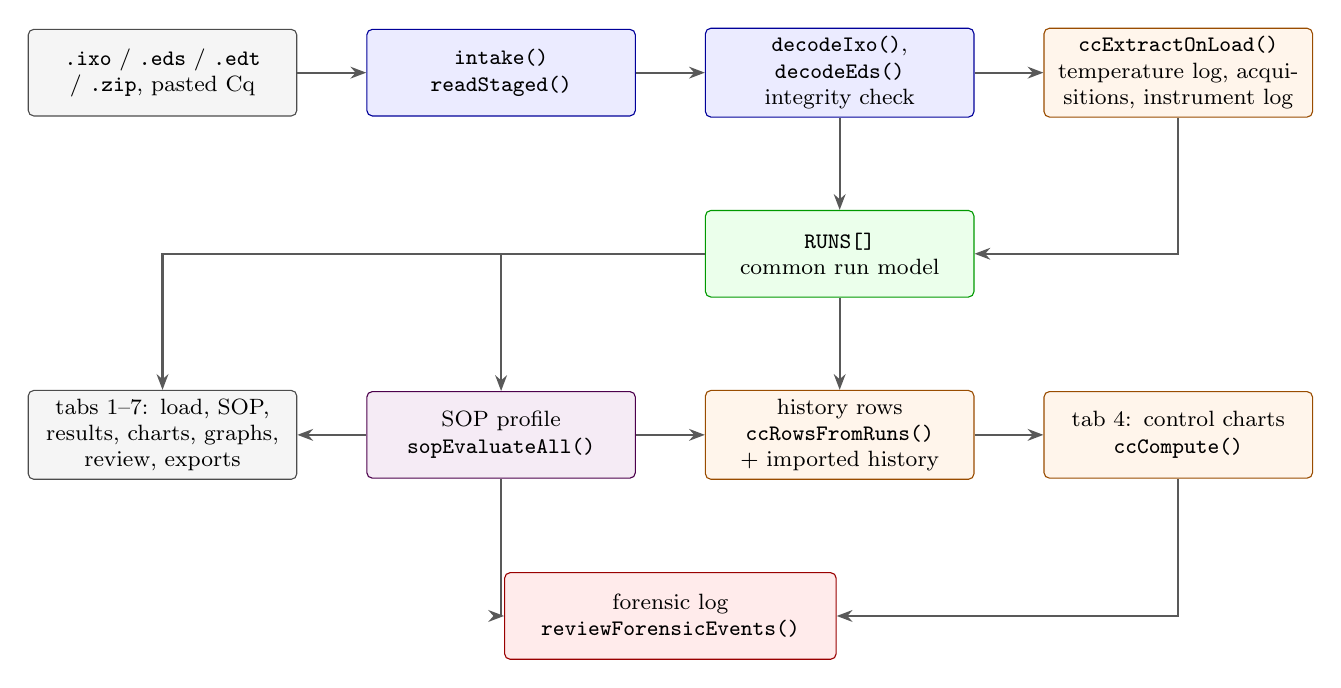
\begin{tikzpicture}[font=\footnotesize,
  box/.style={draw,rounded corners=2pt,align=center,fill=#1!8,draw=#1!60!black,minimum height=11mm,text width=3.2cm,inner sep=3pt},
  box/.default=blue, arr/.style={-{Stealth[length=2mm]},thick,gray!70!black}]
\node[box=gray]   (files)    at (0,0)      {\texttt{.ixo} / \texttt{.eds} / \texttt{.edt} / \texttt{.zip}, pasted Cq};
\node[box]        (intake)   at (4.3,0)    {\texttt{intake()}\\\texttt{readStaged()}};
\node[box]        (dec)      at (8.6,0)    {\texttt{decodeIxo()}, \texttt{decodeEds()}\\integrity check};
\node[box=orange] (cc)       at (12.9,0)   {\texttt{ccExtractOnLoad()}\\temperature log, acquisitions, instrument log};
\node[box=green]  (runs)     at (8.6,-2.3) {\texttt{RUNS[]}\\common run model};
\node[box=gray]   (tabs)     at (0,-4.6)   {tabs 1--7: load, SOP, results, charts, graphs, review, exports};
\node[box=violet] (sop)      at (4.3,-4.6) {SOP profile\\\texttt{sopEvaluateAll()}};
\node[box=orange] (rows)     at (8.6,-4.6) {history rows\\\texttt{ccRowsFromRuns()}\\+ imported history};
\node[box=orange] (panel)    at (12.9,-4.6){tab 4: control charts\\\texttt{ccCompute()}};
\node[box=red,text width=4cm] (forensic) at (6.45,-6.9){forensic log\\\texttt{reviewForensicEvents()}};
\draw[arr] (files)--(intake); \draw[arr] (intake)--(dec); \draw[arr] (dec)--(cc);
\draw[arr] (dec)--(runs); \draw[arr] (cc)|-(runs);
\draw[arr] (runs)-|(sop); \draw[arr] (runs)--(rows); \draw[arr] (sop)--(rows); \draw[arr] (rows)--(panel);
\draw[arr] (sop)--(tabs); \draw[arr] (runs)-|(tabs);
\draw[arr] (sop)|-(forensic); \draw[arr] (panel)|-(forensic);
\end{tikzpicture}
\caption{Data flow. The raw bytes are read once; the instrument-side numbers are extracted while the bytes are in memory, so
later steps never need the file again.}\label{fig:flow}
\end{figure}

Two design rules follow from the size of real data sets (100+ files of 2--11~MB each):
\begin{itemize}
\item \textbf{Read once, keep only what is needed.} The decoders keep the decoded values and a thinned copy of the temperature
      log (1\,800 slices); the raw XML and ZIP bytes are not kept for display.
\item \textbf{Render lazily.} A tab is drawn only when it is opened and only if its inputs changed (\texttt{markDirty}).
\end{itemize}

The delivered script also keeps an explicit lifecycle record. File intake, decoding/SOP evaluation and rendering/export are
separate boundaries even though they share one HTML file. A generation token invalidates a pending read when a newer selection
arrives; a decoder result is checked for the common run shape before it reaches a chart; and the last 100 failures are retained
as structured diagnostic events. Intake reports a 512-file and 2~GiB staging limit instead of silently dropping input. These
checks make a slow or malformed input observable while leaving stored Cq values and calls unchanged.

\par\medskip\noindent{\small\textbf{Listing}~\texttt{markDirty()}\hfill\textcolor{gray}{HTML lines 5498--5498}}\par\nopagebreak
\lstinputlisting[style=vstyle,language=JavaScript,firstnumber=5498]{code/markDirty.js}


\par\medskip\noindent{\small\textbf{Listing}~\texttt{renderTab()}\hfill\textcolor{gray}{HTML lines 5504--5525}}\par\nopagebreak
\lstinputlisting[style=vstyle,language=JavaScript,firstnumber=5504]{code/renderTab.js}


\par\medskip\noindent{\small\textbf{Listing}~\texttt{showTab()}\hfill\textcolor{gray}{HTML lines 10203--10209}}\par\nopagebreak
\lstinputlisting[style=vstyle,language=JavaScript,firstnumber=10203]{code/showTab.js}


\par\medskip\noindent{\small\textbf{Listing}~\texttt{refreshAll()}\hfill\textcolor{gray}{HTML lines 10195--10202}}\par\nopagebreak
\lstinputlisting[style=vstyle,language=JavaScript,firstnumber=10195]{code/refreshAll.js}



\section{The common run model}
Both decoders return the same object, so every later step works on either instrument. Its main members are:
\begin{center}\small
\begin{tabular}{@{}lp{11.5cm}@{}}\toprule
Member & Content\\\midrule
\texttt{meta} & name, creation, run start and end, last change, operator, software and instrument version, instrument ID\\
\texttt{wells[]} & one entry per well and analysis: sample, target, channel and filter pair, role, stored Cq (\texttt{Cp}), call, curve\\
\texttt{allCurves} & every acquired curve, analysed or not (\texttt{"channel|position"})\\
\texttt{plate}, \texttt{subsets}, \texttt{analyses} & plate layout, named subsets, analysis settings and dates\\
\texttt{protocol} & programs, segments (target, hold, ramp, acquisition), channels, block\\
\texttt{integrity} & stored and computed container checksum (.ixo instrument) or tamper value (.eds instrument)\\
\texttt{eds} & .eds instrument only: log, calibrations, per-image data, results tables\\
\texttt{cc}, \texttt{ccStatic} & control-panel extraction (Chapter~\ref{ch:panel})\\\bottomrule
\end{tabular}
\end{center}




\dnasep
\chapter{Tab 1 · Load files: reading and decoding}\label{ch:load}

\figui{ui_start.png}{The page before any file is read.}{ui_start}

\section{File intake}
Files arrive by drag and drop or the file dialog. \texttt{intake()} sorts them by extension (a \texttt{.zip} is opened and searched
for \texttt{.ixo}, \texttt{.eds} and \texttt{.edt} entries), decodes .ixo instrument XML text once, and lists what will be read.
\texttt{readStaged()} then decodes each file, runs the control-panel extraction while the bytes are still in memory and
opens the Control panel.

\par\medskip\noindent{\small\textbf{Listing}~\texttt{intake()}\hfill\textcolor{gray}{HTML lines 9993--10062}}\par\nopagebreak
\lstinputlisting[style=vstyle,language=JavaScript,firstnumber=9993]{code/intake.js}


\par\medskip\noindent{\small\textbf{Listing}~\texttt{readStaged()}\hfill\textcolor{gray}{HTML lines 10063--10073}}\par\nopagebreak
\lstinputlisting[style=vstyle,language=JavaScript,firstnumber=10063]{code/readStaged.js}



\figui[0.9]{ui_load.png}{Load tab after reading: the synthetic data set notice and the \emph{What was read} table (one row per run).}{ui_load}

\section{.ixo instrument (\texttt{.ixo})}
An \texttt{.ixo} file is XML. Objects (\texttt{<obj>}) carry properties (\texttt{<prop name="\dots">}); binary members are base64.
The decoder reads the plate model, subsets, protocol, analyses, results and the raw acquisitions.

\par\medskip\noindent{\small\textbf{Listing}~\texttt{decodeIxo() — opening part}\hfill\textcolor{gray}{HTML lines 2687--3029}}\par\nopagebreak
\lstinputlisting[style=vstyle,language=JavaScript,firstnumber=2687]{code/decodeIxo.js}



\subsection*{Container integrity}
The file stores a checksum of its content. \texttt{ixoIntegrity()} recomputes it; a mismatch means the XML was edited
outside the instrument software and is reported as an error in the forensic log.

\par\medskip\noindent{\small\textbf{Listing}~\texttt{ixoIntegrity()}\hfill\textcolor{gray}{HTML lines 3742--3756}}\par\nopagebreak
\lstinputlisting[style=vstyle,language=JavaScript,firstnumber=3742]{code/ixoIntegrity.js}



\subsection*{Block temperature log (\texttt{TemperatureLog})}
The block temperature is logged about every 0.41\,s for the whole run. Two arrays are stored: \texttt{Times} with the magic
\texttt{LARZ} (uint32 milliseconds) and \texttt{Temps} with \texttt{DARZ} (float64 °C). After a short header the values are
either raw or compressed with LZSS (4\,096-byte ring buffer, matches of 3--18 bytes, one flag bit per item).

\begin{infobox}
The header length varies between files (12 or 13 bytes were found). Reading from the wrong offset produced temperatures such as
$10^{102}$\,°C for one interrupted run, which distorted every thermal metric of that run. \texttt{ccDecodeArz()} therefore
tries every plausible start and keeps the one whose \emph{whole} array is physically plausible (temperatures $-50$\dots$200$\,°C,
times never decreasing); \texttt{ccIxoTemperatureLog()} drops any point that is still implausible.
\end{infobox}

\par\medskip\noindent{\small\textbf{Listing}~\texttt{ccLzss()}\hfill\textcolor{gray}{HTML lines 5545--5559}}\par\nopagebreak
\lstinputlisting[style=vstyle,language=JavaScript,firstnumber=5545]{code/ccLzss.js}


\par\medskip\noindent{\small\textbf{Listing}~\texttt{ccDecodeArz()}\hfill\textcolor{gray}{HTML lines 5560--5573}}\par\nopagebreak
\lstinputlisting[style=vstyle,language=JavaScript,firstnumber=5560]{code/ccDecodeArz.js}


\par\medskip\noindent{\small\textbf{Listing}~\texttt{ccIxoTemperatureLog()}\hfill\textcolor{gray}{HTML lines 5574--5582}}\par\nopagebreak
\lstinputlisting[style=vstyle,language=JavaScript,firstnumber=5574]{code/ccIxoTemperatureLog.js}



\subsection*{Fluorescence acquisitions (\texttt{AcquisitionStore})}
Every fluorescence reading is a record with its time, the block temperature at that moment (hexadecimal big-endian double),
the channel, the automatic integration time, a validity flag and the lamp reference value. The store is deflate-compressed XML.

\par\medskip\noindent{\small\textbf{Listing}~\texttt{ccIxoAcquisitions()}\hfill\textcolor{gray}{HTML lines 5585--5592}}\par\nopagebreak
\lstinputlisting[style=vstyle,language=JavaScript,firstnumber=5585]{code/ccIxoAcquisitions.js}



\section{.eds/.edt instrument (\texttt{.eds}, \texttt{.edt})}
An \texttt{.eds} file is a ZIP container. \texttt{parseEds()} checks the CRC of every entry and the tamper value written by the
instrument software, then reads the experiment description, plate, protocol, analysis results, multicomponent and raw data,
calibrations, the per-image \texttt{quant} files and the instrument's \texttt{messages.log}. \texttt{decodeEds()} maps the result
onto the common run model.

\par\medskip\noindent{\small\textbf{Listing}~\texttt{parseEds() — opening part}\hfill\textcolor{gray}{HTML lines 3181--3387}}\par\nopagebreak
\lstinputlisting[style=vstyle,language=JavaScript,firstnumber=3181]{code/parseEds.js}


\par\medskip\noindent{\small\textbf{Listing}~\texttt{decodeEds() — opening part}\hfill\textcolor{gray}{HTML lines 3611--3739}}\par\nopagebreak
\lstinputlisting[style=vstyle,language=JavaScript,firstnumber=3611]{code/decodeEds.js}



\subsection*{Instrument log and Ct re-derivation}
\texttt{parseLog()} reads the once-per-second \texttt{Temperature} and \texttt{LEDStatus} lines. \texttt{recalcCt()} re-derives
every Ct from the stored $\Delta$Rn and threshold, so a stored Ct that does not match its own curve can be flagged.

\par\medskip\noindent{\small\textbf{Listing}~\texttt{parseLog()}\hfill\textcolor{gray}{HTML lines 3397--3413}}\par\nopagebreak
\lstinputlisting[style=vstyle,language=JavaScript,firstnumber=3397]{code/parseLog.js}


\par\medskip\noindent{\small\textbf{Listing}~\texttt{recalcCt()}\hfill\textcolor{gray}{HTML lines 3391--3395}}\par\nopagebreak
\lstinputlisting[style=vstyle,language=JavaScript,firstnumber=3391]{code/recalcCt.js}



\texttt{ccQsLog()} makes one more pass over the log for the timing and mechanics used by the control panel: command reply times,
camera and filter-wheel moves, encoder offsets, heated-cover drive, scheduler lateness, image processing, predicted and actual
run time, errors and the lifetime counters of the block.

\par\medskip\noindent{\small\textbf{Listing}~\texttt{ccQsLog()}\hfill\textcolor{gray}{HTML lines 5712--5752}}\par\nopagebreak
\lstinputlisting[style=vstyle,language=JavaScript,firstnumber=5712]{code/ccQsLog.js}



\section{What each file type carries}
\begin{center}\small
\begin{tabular}{@{}p{4.6cm}p{4.9cm}p{5.6cm}@{}}\toprule
Information & .ixo instrument (\texttt{.ixo}) & .eds/.edt instrument (\texttt{.eds})\\\midrule
Block temperature & \texttt{TemperatureLog}, 0.41\,s, block & \texttt{messages.log}, 1\,s, modelled sample temperature, 6 zones, cover, heat sink\\
Temperature at each reading & every acquisition record & every image (6 zones)\\
Light source & lamp reference channel per reading & LED temperature, current, voltage, junction\\
Exposure & automatic integration time per reading & requested exposure per image\\
Mechanics & channel switch timing & filter wheel, encoder, heated cover\\
Embedded computer & -- & command replies, 1-s timer, scheduler, image processing\\
Calibrations & -- & uniformity, background, ROI files\\
Lifetime counters & -- & block cycles, degrees climbed\\
Not in the file & lamp hours, plate loading, error log (Instrument Problem Report) & drawer and plate insertion, LED hours\\\bottomrule
\end{tabular}
\end{center}

\section{Extraction for the control panel}
\texttt{ccExtractOnLoad()} runs once per file during reading and stores the extracted instrument numbers on the run, together
with a thinned copy of the temperature log for display.

\par\medskip\noindent{\small\textbf{Listing}~\texttt{ccExtractOnLoad()}\hfill\textcolor{gray}{HTML lines 5901--5920}}\par\nopagebreak
\lstinputlisting[style=vstyle,language=JavaScript,firstnumber=5901]{code/ccExtractOnLoad.js}





\chapter{Tab 2 · SOP: the laboratory's rules as a profile}\label{ch:sop}

The separate Tab~3 (Results) uses the same active profile. It is opened automatically after files are read, so the
interpretation table follows the loading step while the editable profile remains in this tab.

\section{The SOP profile}
Interpretation rules differ between laboratories and methods. The page keeps them in one \textbf{SOP profile}, a JSON document
(schema \texttt{qpcr-sop-profile/1}) that can be edited on the page, saved, locked and reopened. The stored Cq values and calls
are never changed; every outcome says which rule produced it, and every export carries the profile's name, version and SHA-256.

\begin{center}\small
\begin{tabular}{@{}lp{11.6cm}@{}}\toprule
Section & Content\\\midrule
1 · Identity & name, version, author or approver, assay, effective date, notes\\
2 · Targets & target patterns (exact, wildcard or regular expression), kind (target, reference, internal control), Cq cut-off, late-signal limit, minimum quantity, outcome in the late zone\\
3 · Controls & how controls are recognised (by role or by sample name), expected result (negative, positive with a Cq range, standard), purpose, material, minimum replicate wells per group, minimum groups per run, action on failure\\
4 · Replicates \& IC & minimum replicates, replicates needed for a positive, maximum SD, internal-control shift and fixed reference Cq\\
5 · Run acceptance & integrity, missing or failed controls, standard-curve R$^2$ and efficiency, NTC gap, edit delay, calibration, zone spread, run state\\
6 · Outcomes & labels, colours and the report sentence of each outcome\\
7 · Graph settings & which SOP lines are drawn\\
8 · Control charts & per-chart settings of the Control panel (\texttt{controlCharts})\\\bottomrule
\end{tabular}
\end{center}

The SC figures use the generated review profile \emph{SC screening -- SOP-06 laboratory default}, version 1.0. It is review-only until the laboratory approves the mapping and the unresolved comparison direction in SOP-06 section 6.2(c5). The profile recognises 35S and T-NOS targets, HMG or LEC reference targets, 415B and 410CP LOD controls, NTC, process blanks and negative maize or soy controls. This abbreviated JSON shows the profile shape; values are synthetic configuration examples:

\begin{lstlisting}[style=vstyle,language=json, numbers=left,firstnumber=1]
{ "schema": "qpcr-sop-profile/1", "name": "SC screening -- SOP-06 laboratory default", "version": "1.0",
  "author": "Demo QA manager",
  "targets": [ {"match": "HMG|hmg|lec|Le1|ADH|adh1|SSIIb|zSSIIb|Cru|cruA|GLP", "kind": "reference",
                "cqMax": 40, "cqLate": 36, "lateOutcome": "Inconclusive"},
               {"match": "*", "kind": "target", "cqMax": 40, "cqLate": 38, "lateOutcome": "Repeat"} ],
  "controls": [ {"name": "415B LOD control", "matchBy": "name", "match": "/^415B(?=\\b|\\d)/i",
                 "targets": "35S|TNOS|T-NOS", "expect": "positive", "purpose": "LOD control",
                 "cqLo": 29, "cqHi": 36, "minReplicates": 2, "minPerRun": 0, "onFail": "review"},
                {"name": "Extraction blank", "matchBy": "name", "match": "/^(BLANK|BLK)\\s*EX/i",
                 "expect": "negative", "purpose": "extraction blank", "minReplicates": 1,
                 "minPerRun": 0, "onFail": "review"} ],
  "replicates": {"min": 2, "positiveMin": 2, "partialOutcome": "Repeat", "maxSd": 0.5, "sdOutcome": "Repeat"},
  "run": {"integrity": "reject", "controlsFail": "reject", "editDelayHours": 72, "editAction": "review", "…": "…"},
  "controlCharts": {"cool_rate": {"x": "date", "baseFrom": "2025-05-12"}, "transition": {"x": "date"}},
  "sha256": "…" }
\end{lstlisting}

\par\medskip\noindent{\small\textbf{Listing}~\texttt{sopBase()}\hfill\textcolor{gray}{HTML lines 4095--4111}}\par\nopagebreak
\lstinputlisting[style=vstyle,language=JavaScript,firstnumber=4095]{code/sopBase.js}


\par\medskip\noindent{\small\textbf{Listing}~\texttt{SOP\_PRESETS()}\hfill\textcolor{gray}{HTML lines 4112--4139}}\par\nopagebreak
\lstinputlisting[style=vstyle,language=JavaScript,firstnumber=4112]{code/SOP_PRESETS.js}



\textbf{Which starting point the page offers.} \texttt{Start from} now lists only \emph{SC screening — SOP-06 laboratory
default} (\texttt{SOP\_PRESETS.sc}), and a session with no stored profile starts from it. The earlier generic, GMO and
forensic templates remain in the source as scaffolds used by the review mapping (\texttt{sopLabScreening}), but they are not
offered in the selector and a stored profile recognised as one of those templates is replaced by the SC default when only
\texttt{SC\_} experiments are loaded. Opening a file with the review schema
\texttt{qpcr-control-mapping-proposal/v1} converts it to the SC profile shape; the raw names, stored Cq values, calls and
dates are untouched.

\section{Integrity of the profile}
The SHA-256 is computed over a canonical form of the profile (keys sorted, the fields \texttt{sha256} and \texttt{locked} left
out). Any change of any rule, including a control-chart setting, changes the hash, which is printed on every graph and export.

\par\medskip\noindent{\small\textbf{Listing}~\texttt{sopCanonical()}\hfill\textcolor{gray}{HTML lines 4239--4242}}\par\nopagebreak
\lstinputlisting[style=vstyle,language=JavaScript,firstnumber=4239]{code/sopCanonical.js}


\par\medskip\noindent{\small\textbf{Listing}~\texttt{sopHash()}\hfill\textcolor{gray}{HTML lines 4243--4243}}\par\nopagebreak
\lstinputlisting[style=vstyle,language=JavaScript,firstnumber=4243]{code/sopHash.js}



\figui[0.8]{ui_sop.png}{SOP \& results tab: profile header with version and SHA-256, sections 1--2 of the editor; sections 3--8 are folded.}{ui_sop}

\section{Evaluating a run}
\texttt{sopEvaluateRun()} groups the wells by sample and target, recognises controls, applies cut-offs, late-signal limits,
replicate rules and the internal control, and then the run-acceptance criteria. A run that fails a criterion set to
\emph{reject} turns all its sample results into \emph{Invalid run}. In the synthetic data set the planted contaminated extraction
blank of run 022 does exactly this (Figure~\ref{fig:g_LCX_curves}).

\par\medskip\noindent{\small\textbf{Listing}~\texttt{sopMatcher()}\hfill\textcolor{gray}{HTML lines 4248--4254}}\par\nopagebreak
\lstinputlisting[style=vstyle,language=JavaScript,firstnumber=4248]{code/sopMatcher.js}


\par\medskip\noindent{\small\textbf{Listing}~\texttt{sopEvaluateRun() — opening part}\hfill\textcolor{gray}{HTML lines 4434--4570}}\par\nopagebreak
\lstinputlisting[style=vstyle,language=JavaScript,firstnumber=4434]{code/sopEvaluateRun.js}



\section{Dates and the run timeline}
Every dated event in a file (experiment created, run started and ended, analyses created and modified, last change; for
.eds instrument also the ZIP entry dates, instrument log and calibrations) becomes a timeline. The edit delay and the run duration
used by the SOP and the control panel come from it.

\par\medskip\noindent{\small\textbf{Listing}~\texttt{sopTime()}\hfill\textcolor{gray}{HTML lines 4370--4374}}\par\nopagebreak
\lstinputlisting[style=vstyle,language=JavaScript,firstnumber=4370]{code/sopTime.js}


\par\medskip\noindent{\small\textbf{Listing}~\texttt{runTimeline()}\hfill\textcolor{gray}{HTML lines 4387--4407}}\par\nopagebreak
\lstinputlisting[style=vstyle,language=JavaScript,firstnumber=4387]{code/runTimeline.js}


\par\medskip\noindent{\small\textbf{Listing}~\texttt{runTimes()}\hfill\textcolor{gray}{HTML lines 4408--4415}}\par\nopagebreak
\lstinputlisting[style=vstyle,language=JavaScript,firstnumber=4408]{code/runTimes.js}



\section{SOP findings in the forensic log}
\par\medskip\noindent{\small\textbf{Listing}~\texttt{sopEvents()}\hfill\textcolor{gray}{HTML lines 4623--4635}}\par\nopagebreak
\lstinputlisting[style=vstyle,language=JavaScript,firstnumber=4623]{code/sopEvents.js}





\chapter{Control identity, useful graphs and maintenance associations}\label{ch:identity}

\section{What changed in the 22 September revision}
The earlier demonstration could show empty positive-control charts when the loaded laboratory profile did not identify
the controls. An empty plot is not evidence that control measurements are absent. The corrected page distinguishes
configuration, eligibility and an incomplete statistical baseline. This revision keeps the 58-chart catalogue, removes
misleading pooled limits from the older control overview, and adds three descriptive graphs based on explicit control identity.

\begin{infobox}
The SC mapping is a \textbf{review-only profile}. It supplies candidate name rules; it does not certify the applicable
historical SOP, reference-material concentration, aliquot, or the interpretation of a sample-versus-LOD comparison.
The supplied procedures were used to define synthetic examples, not to execute laboratory work.
\end{infobox}

\section{Identity before statistics}
An ordinary specimen code is not a positive control simply because its vendor role is \emph{Unknown} or \emph{Calibrator}.
The page first matches a configured name rule and target. A negative matrix is expected not to amplify the screening target,
but its endogenous taxon target can amplify. That endogenous signal is a reference check, not automatically a fixed-input
internal positive control and not a blank.

For longitudinal control data the key retains the target, complete normalized material label, extraction date and any
aliquot or dilution suffix. The panel also requires the same instrument, recorded program fingerprint and firmware before
enabling statistical alarms. Matching by a shortened root is available in Review only as a descriptive view.
Different extraction batches are not pooled to estimate one control mean or SD.

The date parser accepts a calendar-valid day.month.four-digit-year label. It rejects impossible dates and malformed years,
and marks an extraction date after the run as inconsistent. It does not repair these labels by guessing. Unknown or invalid
dates are isolated by source in panel control keys. The original text remains visible and exportable.

\par\medskip\noindent{\small\textbf{Listing}~\texttt{sopControlIdentity()}\hfill\textcolor{gray}{HTML lines 4286--4308}}\par\nopagebreak
\lstinputlisting[style=vstyle,language=JavaScript,firstnumber=4286]{code/sopControlIdentity.js}


\par\medskip\noindent{\small\textbf{Listing}~\texttt{ccBaselineNeed()}\hfill\textcolor{gray}{HTML lines 4328--4328}}\par\nopagebreak
\lstinputlisting[style=vstyle,language=JavaScript,firstnumber=4328]{code/ccBaselineNeed.js}



\section{Which graphs are useful}
\begin{longtable}{@{}p{4cm}p{11cm}@{}}
\toprule View & Revised use\\\midrule\endhead
Positive-control Cq & One material, extraction batch, aliquot/dilution, target and instrument/program at a time. Non-detection
must be reviewed alongside the Cq of detected replicates.\\
Negative-control rate & Separate reaction blanks, extraction blanks, grinding/environment blanks and negative matrices.
Each stage has its own positive count and eligible denominator. Legacy pooled history remains explicitly labelled as stage unknown.\\
Endogenous reference & Inspect the biological reference separately; a fixed IC shift needs a configured reference Cq and a
matching IC target. Subtracting each run's own median would hide a common shift.\\
Root-name overview & Exploratory only. The older control graph retains the SOP range but no longer displays pooled mean/SD lines.\\
Thermal and mechanical plots & Compare comparable programs and instrument configurations. A trend is an investigation trigger,
not proof of component wear or a validated remaining-life estimate.\\
Operator funnel & Shows unadjusted event rates and workload. It does not adjust for extraction batch, assay, instrument or
case mix and cannot establish an operator effect.\\
\bottomrule
\end{longtable}

\section{New descriptive associations}
The three new plots use one synthetic control group per run, with detected and total replicate counts retained in their
CSV rows. Colours distinguish instrument, target, full control batch and program. Only finite detected Cq means enter the
scatter plots; missing Cq is not replaced by a cut-off.
\readingnote{These are descriptive associations. Read them with detection counts, program settings and maintenance records;
do not treat a slope as a failure probability.}

\fig{g_all_x_control_batches.png}{Control extraction batches over calendar time. The example deliberately changes from a
March extraction to a July extraction; these are separate series.}{control_batches}

\fig{g_all_x_control_age.png}{Control mean Cq against days since the labelled extraction. Invalid, missing or future
extraction dates are excluded from the plotted age values. The example includes an explicitly simulated age effect.}{control_age}

\fig{g_all_x_control_thermal.png}{Control mean Cq against measured peak cooling rate. Both change with time in this
synthetic example; the association does not distinguish ageing extract from changing cooling performance.}{control_thermal}

\par\medskip\noindent{\small\textbf{Listing}~\texttt{controlBatchRecords()}\hfill\textcolor{gray}{HTML lines 4335--4344}}\par\nopagebreak
\lstinputlisting[style=vstyle,language=JavaScript,firstnumber=4335]{code/controlBatchRecords.js}


\par\medskip\noindent{\small\textbf{Listing}~\texttt{controlBatchGraph()}\hfill\textcolor{gray}{HTML lines 4345--4361}}\par\nopagebreak
\lstinputlisting[style=vstyle,language=JavaScript,firstnumber=4345]{code/controlBatchGraph.js}



No correlation coefficient, significance test or causal score is assigned. Before estimating an equipment effect, match
material and extraction batch, target, dilution, program and analysis settings; inspect run order, service dates and operator
allocation. A prospective verification using a stable reference material is stronger evidence than a pooled correlation.
The current implementation groups by the recorded program string; it does not yet enforce a complete analysis-settings
fingerprint or model reagent lot, operator and extract age jointly.

\section{Baseline and alarm corrections}
Statistical limits and forecasts are suppressed until the configured Phase-I size is available (default 20, minimum configurable
size 5) in a single instrument/program/firmware cohort. Specification checks remain separate from statistical checks.
The default trend fit uses Phase I rather than continually refitting every new point. A zero-event p-chart baseline no longer
silently ignores a later positive event. It is still a simple binomial approximation; sparse-event uncertainty is not modelled
by an exact predictive interval.

The erroneous across-run $R_{4s}$ rule was removed. That rule needs appropriately standardized controls within a run;
adjacent run means are not a substitute. The remaining run rules are descriptive monitoring tools, not validated laboratory
acceptance criteria. Review uses exact names by default and a fixed initial baseline; root grouping cannot raise Westgard alarms.

\section{Demonstration and interpretation limits}
The regenerated set contains 57 synthetic runs and 325 synthetic history rows. Thirty screening runs include 24 runs of
the March control extraction and six of the July extraction. The short July batch intentionally illustrates an incomplete
baseline. Historical summary rows contain no dated positive-control metrics because their synthetic well-level batch identities
are not available. They continue to demonstrate thermal, optical, mechanical and process-stage histories.

The new plots show associations rather than equipment diagnoses. LED current, cover motion, cooling and operator differences
were planted independently by the generator. The maintenance suggestions in the catalogue are hypotheses to investigate.
Calibrated temperature verification, optical reference measurements and service records remain external evidence.



\chapter{Tab 4 · Control panel: control charts for predictive maintenance and quality control}\label{ch:panel}

\section{Idea}
Each run file contains far more than Cq values: the block temperature every 0.41\,s (.ixo instrument) or 1\,s (.eds instrument), the
exposure and lamp or LED values of every reading, the timing of the instrument's embedded computer and mechanics, and the
dates of every change. The control panel turns these numbers into \textbf{one history row per run} and draws
\textbf{58 control charts per instrument}, grouped in four families:

\begin{description}[leftmargin=2.6cm,style=nextline]
\item[1 · Hardware] thermal system, optics, mechanics — predictive maintenance;
\item[2 · Software] embedded computer, analysis software, data integrity;
\item[3 · Method] reagents, probes, assay behaviour;
\item[4 · Operator] pipetting precision, contamination, unadjusted comparisons (funnel plots).
\end{description}

Charts compare an instrument only with itself. Each tile shows a status light for the latest run (green in control, amber
watch, red alarm, grey not enough data), the latest value and a sparkline; a click opens the chart page.

\figui[0.82]{ui_panel_lc1.png}{Control panel for the synthetic .ixo instrument \texttt{LC-DEMO-01} (180 runs: 150 imported history rows and 30 runs built in the page). Summary cards, then the tiles of the hardware, software, method and operator groups.}{ui_panel_lc1}

{\footnotesize
\begin{longtable}{@{}lllll@{}}
\toprule \textbf{Code} & \textbf{Chart} & \textbf{Instr.} & \textbf{Default} & \textbf{Unit} \\\midrule\endfirsthead
\toprule \textbf{Code} & \textbf{Chart} & \textbf{Instr.} & \textbf{Default} & \textbf{Unit} \\\midrule\endhead
\texttt{B-H1} & Peak heating rate (2-s window) & LC QS & Trend & °C/s \\\hline
\texttt{B-H2} & Peak cooling rate (2-s window) & LC QS & Trend & °C/s \\\hline
\texttt{B-H3} & Overshoot at the denaturation step & LC QS & CUSUM & °C \\\hline
\texttt{B-H3b} & Settling time at the denaturation step & LC QS & I-MR & s \\\hline
\texttt{B-H3c} & Transition time A → B °C & LC QS & I-MR & s \\\hline
\texttt{B-H4} & Temperature at the moment of reading & LC QS & X̄–S & °C from setpoint \\\hline
\texttt{B-H5} & Block zone uniformity (95th percentile) & QS & EWMA & °C \\\hline
\texttt{B-H6} & Heat-sink maximum & QS & I-MR & °C \\\hline
\texttt{B-H6b} & Heated cover temperature & QS & I-MR & °C \\\hline
\texttt{B-H8} & Lamp reference channel (stability) & LC & I-MR & reference counts \\\hline
\texttt{B-H9} & Lamp drift within a run & LC & I-MR & \% change in the run \\\hline
\texttt{B-H10} & LED drive current & QS & Trend & current (as logged) \\\hline
\texttt{B-H10b} & LED junction temperature (maximum) & QS & I-MR & °C \\\hline
\texttt{B-H11} & Automatic integration time / exposure & LC QS & I-MR & ms \\\hline
\texttt{B-H12} & Saturated well images & QS & p & share of well images \\\hline
\texttt{B-H13} & Uniformity calibration: edge-to-centre ratio & QS & I-MR & edge / centre \\\hline
\texttt{B-H13b} & Background calibration: mean offset & QS & I-MR & counts \\\hline
\texttt{B-H13c} & Well-position (ROI) calibration: spot diameter & QS & I-MR & pixels \\\hline
\texttt{B-H14} & Filter-wheel move time & QS & I-MR & ms \\\hline
\texttt{B-H14b} & Filter-wheel moves slower than 500 ms & QS & p & share of moves \\\hline
\texttt{B-H15} & Filter-wheel position offset & QS & I-MR & encoder counts \\\hline
\texttt{B-H16} & Camera readout time beyond the exposure & QS & X̄–S & ms \\\hline
\texttt{B-H17} & Channel switch time & LC & I-MR & ms \\\hline
\texttt{B-H18} & Heated cover lowering time & QS & Trend & s \\\hline
\texttt{B-H18b} & Heated cover raising time & QS & I-MR & s \\\hline
\texttt{A-H3} & Background fluorescence per channel & LC QS & I-MR & fluorescence \\\hline
\texttt{A-H3b} & End-point fluorescence per channel & LC QS & I-MR & fluorescence \\\hline
\texttt{A-H4} & Run duration & LC QS & I-MR & minutes \\\hline
\texttt{B-S1} & Reply time to the PC software & QS & I-MR & ms (95th pct) \\\hline
\texttt{B-S2} & Once-per-second timer lateness & QS & I-MR & ms (95th pct) \\\hline
\texttt{B-S2b} & Scheduler falling behind & QS & u & events per run hour \\\hline
\texttt{B-S3} & Image → processing delay & QS & I-MR & ms (95th pct) \\\hline
\texttt{B-S4} & Image analysis time & QS & I-MR & ms \\\hline
\texttt{B-S5} & Run-time prediction error & QS & I-MR & \% \\\hline
\texttt{B-S6} & Data hand-off time & QS & I-MR & minutes \\\hline
\texttt{B-S8} & Command errors in the instrument log & QS & c & errors \\\hline
\texttt{B-S9} & Cycle-timing regularity & LC QS & I-MR & ms \\\hline
\texttt{B-S10} & Temperature-log intervals over 500 ms & LC & p & share of intervals \\\hline
\texttt{B-S11} & Invalid fluorescence readings & LC & p & share of readings \\\hline
\texttt{B-S12} & Stored Ct not reproducible (> 0.2) & QS & p & share of wells \\\hline
\texttt{A-S4} & Run end → last change & LC QS & I-MR & log10 hours \\\hline
\texttt{A-S6} & Forensic findings per run & LC QS & c & findings \\\hline
\texttt{A-M1} & Positive control Cq (Levey-Jennings) & LC QS & I-MR & Cq \\\hline
\texttt{B-M1} & Probe signal strength (positive control) & LC QS & EWMA & fluorescence \\\hline
\texttt{B-M2} & Passive reference (ROX) level & QS & I-MR & passive reference \\\hline
\texttt{B-M3} & PCR efficiency from the standards & LC QS & Trend & \% efficiency \\\hline
\texttt{B-M5} & Negative controls by process stage & LC QS & p & share of NTC wells \\\hline
\texttt{B-M6} & IC shift from fixed reference & LC QS & EWMA & cycles \\\hline
\texttt{B-M9} & Low Cq confidence & QS & p & share of wells \\\hline
\texttt{B-M10} & Late signal / stochastic-zone results & LC QS & p & share of results \\\hline
\texttt{B-O1} & Replicate precision (pooled SD, Cq < 30) & LC QS & I-MR & Cq SD \\\hline
\texttt{B-O2} & Dispensed-volume spread (ROX CV) & QS & I-MR & \% CV \\\hline
\texttt{B-O3} & Row / column pattern & LC QS & I-MR & Cq \\\hline
\texttt{B-O5} & Contamination rate by operator (funnel) & LC QS & Funnel & share of NTC wells \\\hline
\texttt{B-O6} & Repeat / inconclusive / invalid rate by operator … & LC QS & Funnel & share of results \\\hline
\texttt{B-O7} & Manual interventions & LC QS & p & share of settings \\\hline
\texttt{B-O9} & Stored calls that disagree with the SOP & LC QS & p & share of wells \\\hline
\texttt{B-O11} & Copied-data events & LC QS & c & events \\\hline
\bottomrule
\end{longtable}}



\section{History rows}
A history row holds everything a chart needs, a few kilobytes per run, so years of runs fit in one JSON file that the
laboratory keeps and re-imports. The key of a row is the SHA-256 of the source file, so the same file is never counted twice.
Hardware and software numbers (\texttt{ccStatic}) are fixed when the file is read; method and operator numbers
(\texttt{ccDynamic}) follow the SOP profile and are recomputed when it changes.

\begin{lstlisting}[style=vstyle,language=json, numbers=left,firstnumber=1]
{ "schema": "qpcr-instrument-history/1", "note": "SYNTHETIC demonstration history — all values are made up",
  "rows": [ { "key": "demo-hist-LC1-0042", "run": "DEMO_LC1_HIST_0043", "platform": "LC",
      "instrument": "LC · LC-DEMO-01", "date": 1718784000000, "operator": "Analyst C",
      "software": "LCS480 1.5.1.62", "firmware": "HTC_VER_10",
      "protocol": "95/600s@4.4 95/15s@4.4 60/60s@2.2 72/1s@4.4 40/30s@2.2",
      "m": { "heat_rate": 4.89, "cool_rate": 2.43, "settling": 6.15,
             "transition": {"95→60 °C": 14.66, "60→72 °C": 2.30, "72→95 °C": 5.74},
             "hold_temp": {"mean": -0.50, "sd": 0.031, "n": 45},
             "ntc_rate": {"extraction blank": {"bad": 1, "n": 6}}, "…": "…" } } ] }
\end{lstlisting}

\par\medskip\noindent{\small\textbf{Listing}~\texttt{ccRowsFromRuns()}\hfill\textcolor{gray}{HTML lines 6332--6346}}\par\nopagebreak
\lstinputlisting[style=vstyle,language=JavaScript,firstnumber=6332]{code/ccRowsFromRuns.js}


\par\medskip\noindent{\small\textbf{Listing}~\texttt{ccStatic()}\hfill\textcolor{gray}{HTML lines 5782--5848}}\par\nopagebreak
\lstinputlisting[style=vstyle,language=JavaScript,firstnumber=5782]{code/ccStatic.js}


\par\medskip\noindent{\small\textbf{Listing}~\texttt{ccDynamic()}\hfill\textcolor{gray}{HTML lines 5850--5899}}\par\nopagebreak
\lstinputlisting[style=vstyle,language=JavaScript,firstnumber=5850]{code/ccDynamic.js}


\par\medskip\noindent{\small\textbf{Listing}~\texttt{ccRowsFor()}\hfill\textcolor{gray}{HTML lines 6352--6357}}\par\nopagebreak
\lstinputlisting[style=vstyle,language=JavaScript,firstnumber=6352]{code/ccRowsFor.js}


\par\medskip\noindent{\small\textbf{Listing}~\texttt{ccImport()}\hfill\textcolor{gray}{HTML lines 6765--6773}}\par\nopagebreak
\lstinputlisting[style=vstyle,language=JavaScript,firstnumber=6765]{code/ccImport.js}


\par\medskip\noindent{\small\textbf{Listing}~\texttt{ccHistoryJSON()}\hfill\textcolor{gray}{HTML lines 6739--6743}}\par\nopagebreak
\lstinputlisting[style=vstyle,language=JavaScript,firstnumber=6739]{code/ccHistoryJSON.js}



\section{Instrument numbers from the temperature log}

\subsection*{Program fingerprint}
Thermal numbers are comparable only between runs of the same program. Every run gets a fingerprint
(\texttt{target/hold@ramp} per segment) and the panel can be restricted to one program.

\par\medskip\noindent{\small\textbf{Listing}~\texttt{ccSetpoints()}\hfill\textcolor{gray}{HTML lines 5706--5709}}\par\nopagebreak
\lstinputlisting[style=vstyle,language=JavaScript,firstnumber=5706]{code/ccSetpoints.js}


\par\medskip\noindent{\small\textbf{Listing}~\texttt{ccProtocolKey()}\hfill\textcolor{gray}{HTML lines 5924--5927}}\par\nopagebreak
\lstinputlisting[style=vstyle,language=JavaScript,firstnumber=5924]{code/ccProtocolKey.js}



\subsection*{Peak ramp rates, overshoot and settling}
The steepest 2-second slope of each transition, median over the run, is independent of plateau detection.
\texttt{ccThermalSteps()} finds the plateaus at the programmed setpoints and measures overshoot and settling time
(from the 90\,\% point until the block stays within $\pm0.5$\,°C).

\par\medskip\noindent{\small\textbf{Listing}~\texttt{ccPeakRates()}\hfill\textcolor{gray}{HTML lines 5684--5696}}\par\nopagebreak
\lstinputlisting[style=vstyle,language=JavaScript,firstnumber=5684]{code/ccPeakRates.js}


\par\medskip\noindent{\small\textbf{Listing}~\texttt{ccThermalSteps()}\hfill\textcolor{gray}{HTML lines 5595--5627}}\par\nopagebreak
\lstinputlisting[style=vstyle,language=JavaScript,firstnumber=5595]{code/ccThermalSteps.js}


\par\medskip\noindent{\small\textbf{Listing}~\texttt{ccThermalSummary()}\hfill\textcolor{gray}{HTML lines 5697--5705}}\par\nopagebreak
\lstinputlisting[style=vstyle,language=JavaScript,firstnumber=5697]{code/ccThermalSummary.js}



\subsection*{Transition time A $\to$ B}
The time from leaving $\pm0.5$\,°C of the start temperature until the block is within $\pm0.5$\,°C of the target, for every
transition the program asks for. Band crossings are interpolated between samples (at 4.4\,°C/s the .ixo instrument moves about
1.8\,°C between two samples, more than the band); passing through another setpoint is ignored, and a hold of at least 2\,s at a
temperature that is not the next step resets the starting point.

\par\medskip\noindent{\small\textbf{Listing}~\texttt{ccTransitionPairs()}\hfill\textcolor{gray}{HTML lines 5635--5646}}\par\nopagebreak
\lstinputlisting[style=vstyle,language=JavaScript,firstnumber=5635]{code/ccTransitionPairs.js}


\par\medskip\noindent{\small\textbf{Listing}~\texttt{ccTransitions()}\hfill\textcolor{gray}{HTML lines 5647--5673}}\par\nopagebreak
\lstinputlisting[style=vstyle,language=JavaScript,firstnumber=5647]{code/ccTransitions.js}


\par\medskip\noindent{\small\textbf{Listing}~\texttt{ccThin()}\hfill\textcolor{gray}{HTML lines 5676--5683}}\par\nopagebreak
\lstinputlisting[style=vstyle,language=JavaScript,firstnumber=5676]{code/ccThin.js}



\section{Statistics}\label{sec:stats}
All limits come from a \textbf{baseline} (Phase~I): the first $n$ runs (default 20; the full configured baseline is required before statistical alarms), or the runs from a
\emph{baseline start date} onwards (after a service). Runs before that date are drawn grey without limits.

\par\medskip\noindent{\small\textbf{Listing}~\texttt{ccPhase()}\hfill\textcolor{gray}{HTML lines 6143--6143}}\par\nopagebreak
\lstinputlisting[style=vstyle,language=JavaScript,firstnumber=6143]{code/ccPhase.js}



\subsection{Individuals chart (I-MR) and run rules}
With $\bar x$ the baseline mean and $\overline{MR}$ the mean moving range,
\[ \hat\sigma=\max\!\Big(\frac{\overline{MR}}{1.128},\ \frac{r}{2}\Big),\qquad \text{limits } \bar x\pm3\hat\sigma , \]
where $r$ is the measurement resolution of quantised values (0.41\,s log samples, 10\,ms channel switch), so a baseline of
identical values does not give $\hat\sigma=0$. Western Electric rules 2--5 (2 of 3 beyond $2\sigma$, 4 of 5 beyond $1\sigma$,
8 on one side, 6 rising or falling) are switchable per chart.

\par\medskip\noindent{\small\textbf{Listing}~\texttt{ccI()}\hfill\textcolor{gray}{HTML lines 6145--6157}}\par\nopagebreak
\lstinputlisting[style=vstyle,language=JavaScript,firstnumber=6145]{code/ccI.js}



\fig[0.9]{cc_wheel_ms.png}{I chart, .eds instrument \texttt{QS-DEMO-A}, B-H14 filter-wheel move time. The planted step of +14\,ms from 2025-09 puts every later run outside the old limits; the page reports it as one sustained shift (Section~\ref{sec:shift}) instead of an alarm per run.}{wheel}
\fig[0.9]{cc_settling.png}{I chart with resolution floor, B-H3b settling time. The value moves in whole log samples (0.41\,s); the planted service step shortens it by one sample, which is the 3$\sigma$ signal, while values on the centre line raise no pattern rule.}{settling}

\subsection{Signal classes: outside the limits versus a pattern inside them}\label{sec:signals}
A flag is not evidence of the same kind in every case. The page separates two classes, computed from the flag text by
\texttt{ccSignal()}:
\begin{itemize}
\item \textbf{limit signal} — the point itself lies outside a control limit or a specification (beyond $3\sigma$, $1_{3s}$,
      off the trend band, EWMA or CUSUM alarm, above a $p$/$u$/$c$ limit, outside the specification). Drawn \textbf{red};
\item \textbf{rule signal} — the point is inside the limits and belongs to a suspicious pattern (Western Electric 2--5,
      Westgard $2_{2s}$, $4_{1s}$, $10_{\bar x}$). Drawn \textbf{amber}.
\end{itemize}
The tile status is red only for a limit signal, or for a pattern rule on a control material (Westgard charts); a pattern on an
equipment chart gives ``watch''. Tooltips read \emph{outside the limits} or \emph{pattern inside the limits}, and the CSV of
every chart carries a \texttt{signal} column with the class.

\par\medskip\noindent{\small\textbf{Listing}~\texttt{ccSignal()}\hfill\textcolor{gray}{HTML lines 5968--5969}}\par\nopagebreak
\lstinputlisting[style=vstyle,language=JavaScript,firstnumber=5968]{code/ccSignal.js}



Two further rules keep the pattern tests honest:
\begin{itemize}
\item a value that falls on the centre line is on \emph{no} side, so runs of identical values no longer produce ``8 on one
      side'' or $10_{\bar x}$;
\item for quantised series a value closer to the centre than half the resolution step ($r/2$; 0.41\,s for the temperature log)
      counts as on the centre, because it cannot be distinguished from it. The $3\sigma$ test is unchanged (Listing \texttt{ccI()}).
\end{itemize}

Background, plateau, exposure, run length, edit delay, lamp drift and cycle timing follow the plate that was run, not the
instrument. Sustained patterns there mirror the work schedule, so rules 2--5 are off by default for those charts and can be
switched on per chart in the settings.

\par\medskip\noindent{\small\textbf{Listing}~\texttt{CC\_RULES\_OFF, ccCfg()}\hfill\textcolor{gray}{HTML lines 6134--6135}}\par\nopagebreak
\lstinputlisting[style=vstyle,language=JavaScript,firstnumber=6134]{code/ccRulesOff.js}



\begin{figure}[htbp]\centering
\begin{subfigure}{0.49\linewidth}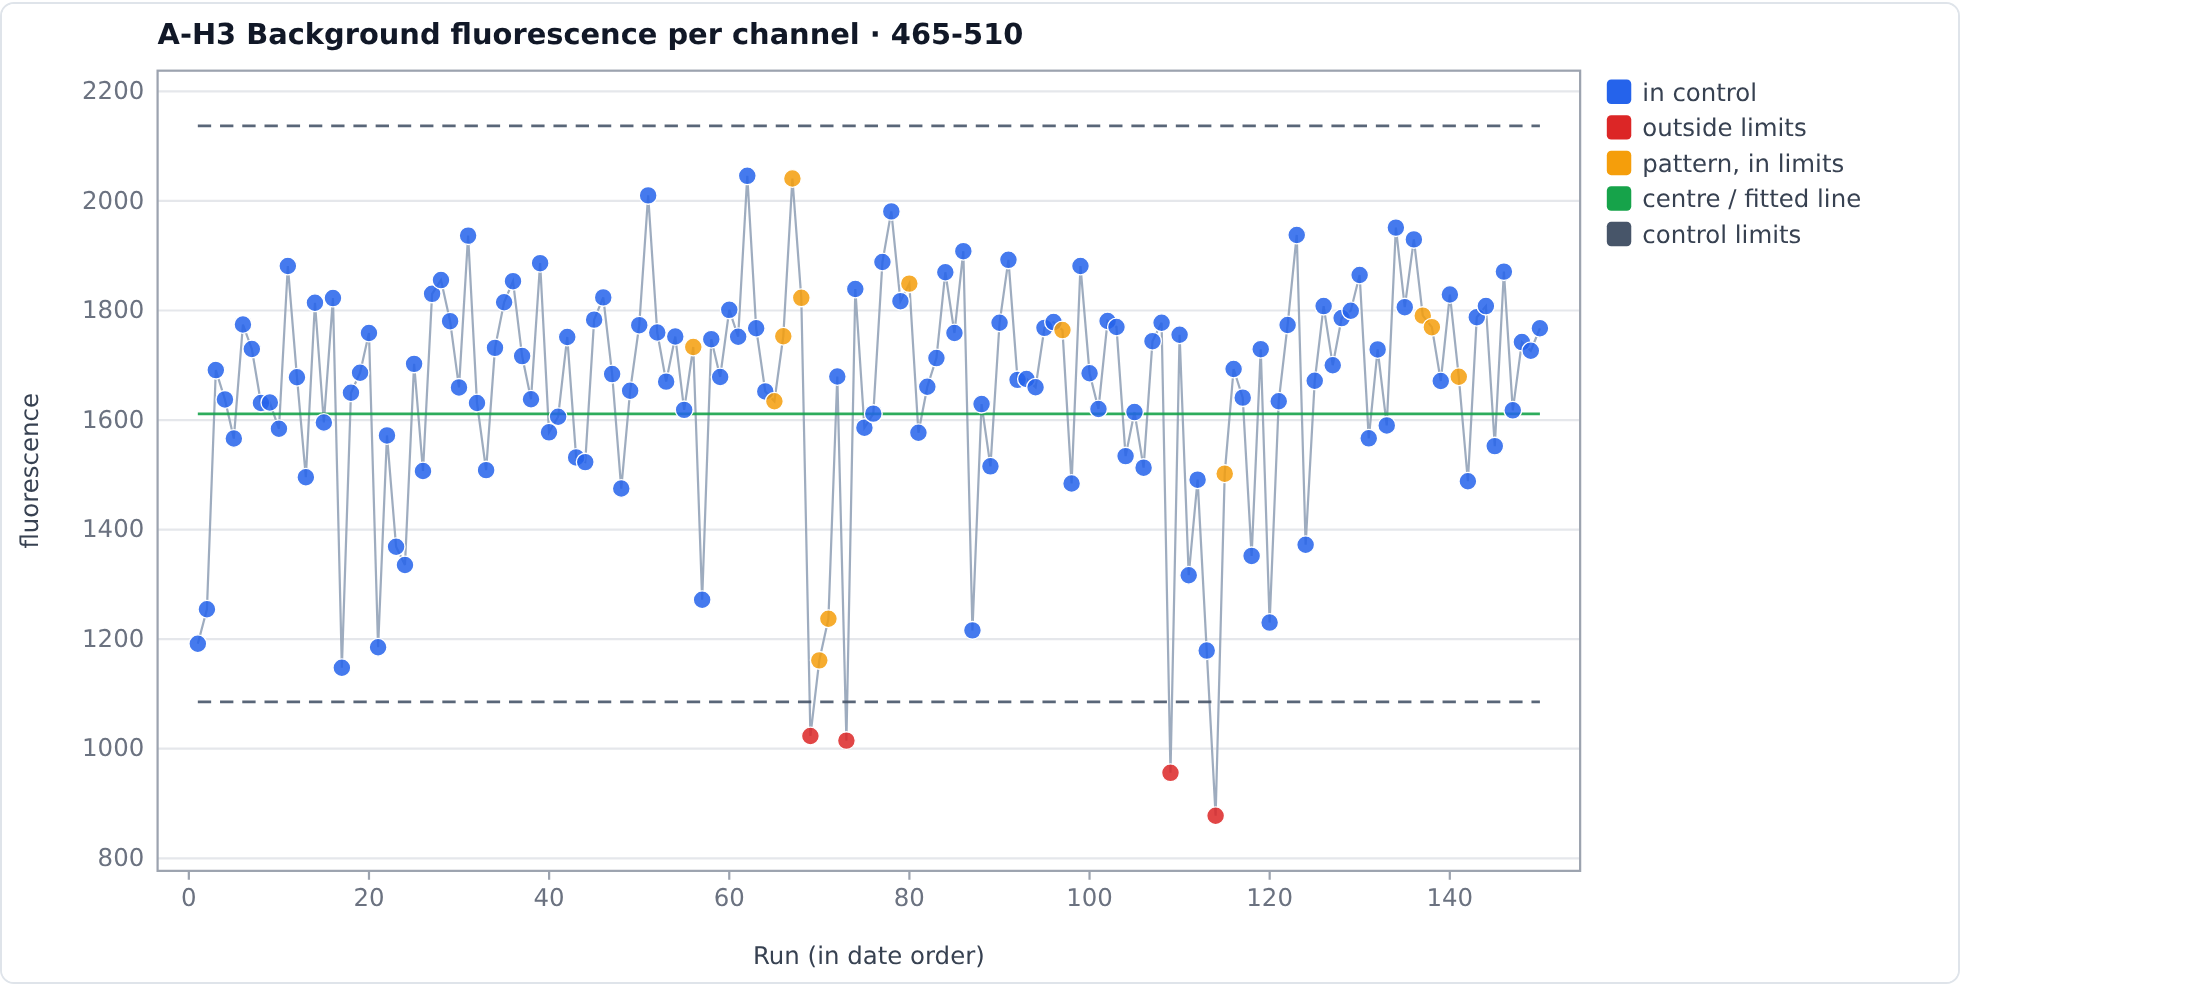
\includegraphics[width=\linewidth]{fig/cc_bg_signal_classes.png}\caption{pattern rules switched on}\label{fig:sig_on}\end{subfigure}\hfill
\begin{subfigure}{0.49\linewidth}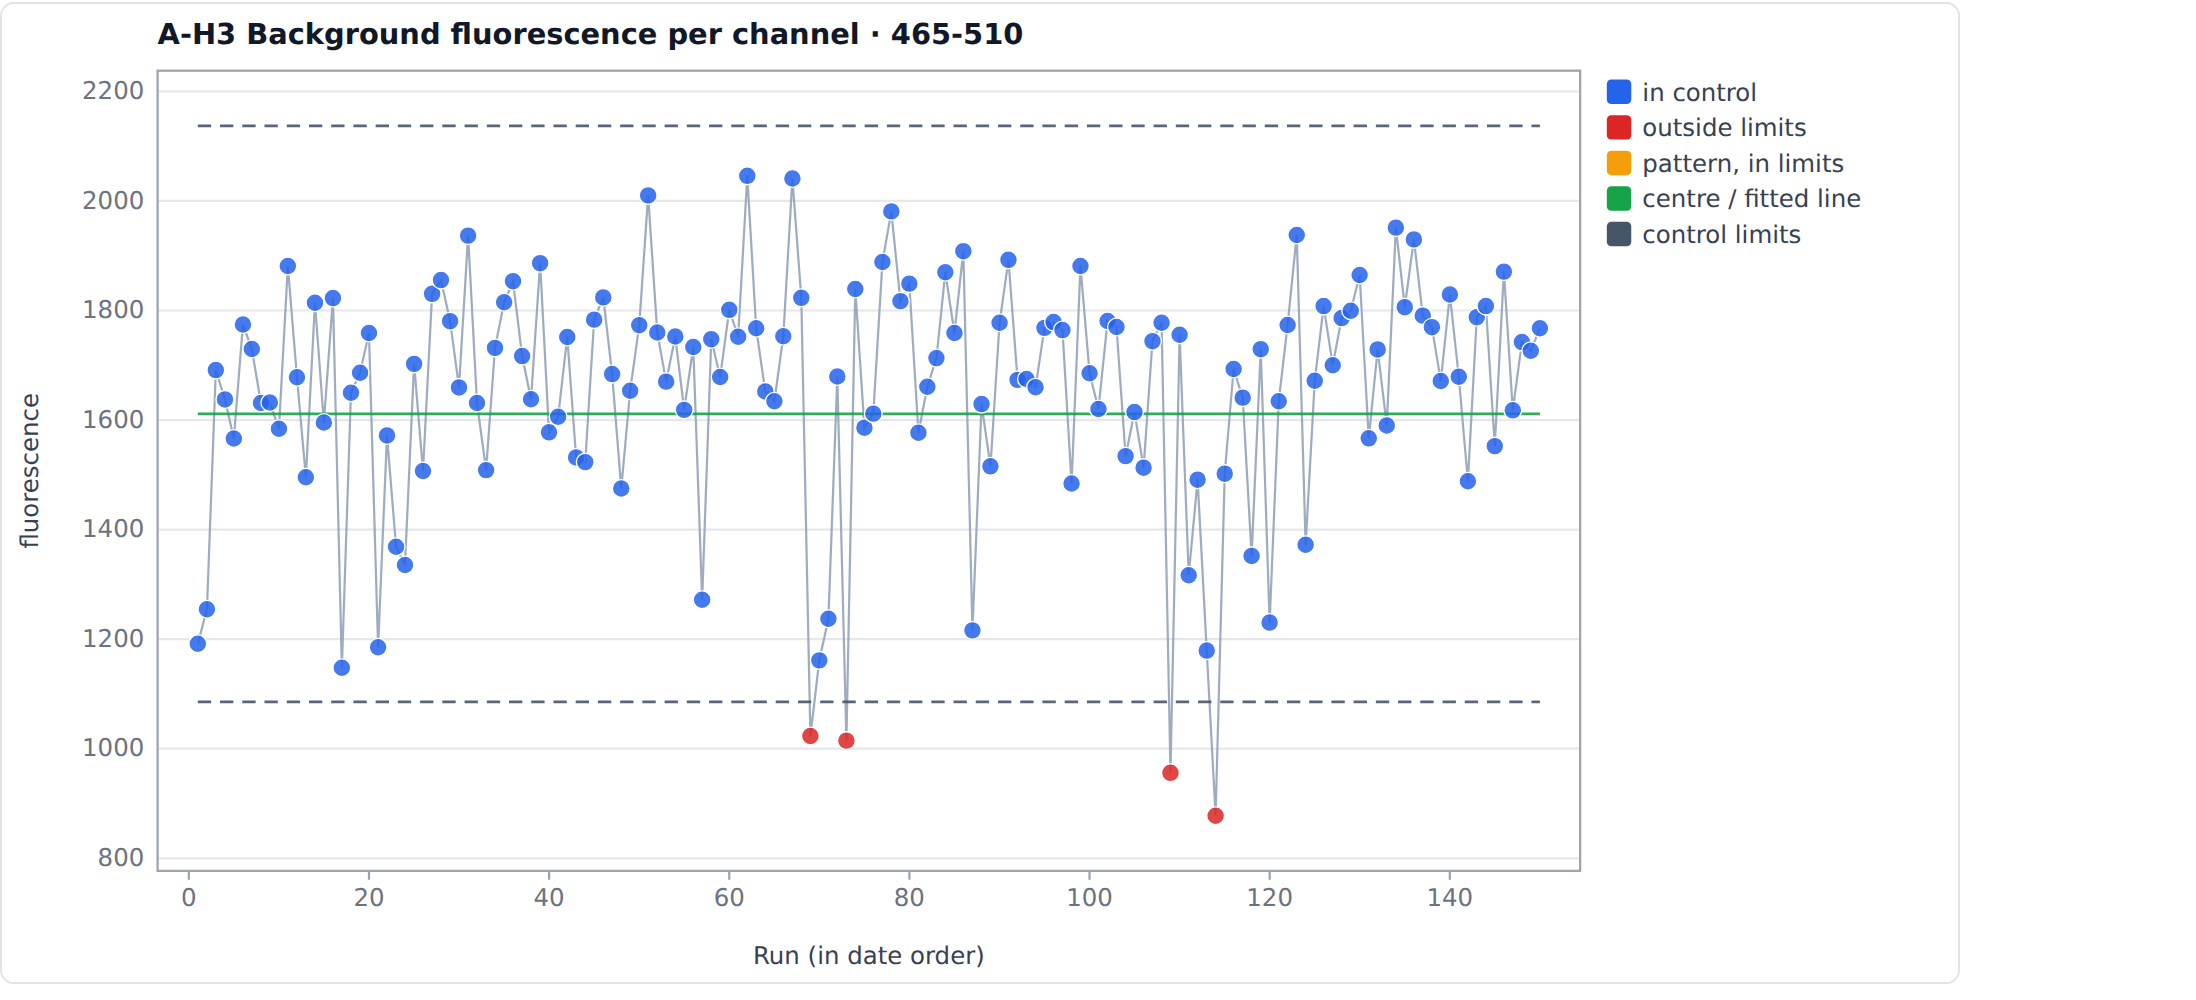
\includegraphics[width=\linewidth]{fig/cc_bg_rules_off.png}\caption{default: only the $3\sigma$ rule}\label{fig:sig_off}\end{subfigure}
\caption{\synthtag A-H3 background fluorescence, LC-DEMO-01, 465-510. In (a) the amber points are inside the control limits and
come from pattern rules; only the four red points are outside a limit. (b) is the default view of the same data.}\label{fig:signals}
\end{figure}
\readingnote{Red asks what happened in that run; amber asks whether the recent plates differ from the baseline period.}

\subsection{Levey-Jennings with Westgard rules}
Control materials use the Westgard multirule on the individuals chart: $1_{3s}$, $2_{2s}$, $4_{1s}$, $10_{\bar x}$. The across-run $R_{4s}$ rule has been removed; it requires a suitable within-run design.
\par\medskip\noindent{\small\textbf{Listing}~\texttt{ccWestgard()}\hfill\textcolor{gray}{HTML lines 6159--6169}}\par\nopagebreak
\lstinputlisting[style=vstyle,language=JavaScript,firstnumber=6159]{code/ccWestgard.js}


\fig[0.9]{cc_pc_cq_35S.png}{A-M1 positive-control Cq, 35S on the demonstration CRM. Each synthetic extract has its own baseline and limits (Section~\ref{sec:extracts}).}{pccq}

\subsection{Control materials: one series per target and material, one segment per extract}\label{sec:extracts}
A positive control is identified by target \emph{and} material (\texttt{35S | 415B}); the extract — extraction date plus any
aliquot or dilution qualifier — is kept separately and becomes a \textbf{segment} of the same chart. Each extract carries its
own baseline and limits, because a new extract is a new process; an extract with fewer runs than the baseline shows no limits
and the tile says how many runs are still missing. Target aliases (\texttt{P35S}/\texttt{35S}, \texttt{TNOS}/\texttt{T-NOS},
\texttt{hmgA}/\texttt{HMG}, \texttt{Le1}/\texttt{LEC}) are merged, and an extraction date later than the run is labelled
\emph{after run} rather than corrected. Histories written before this change are converted on import.

\par\medskip\noindent{\small\textbf{Listing}~\texttt{ccMigrateControlKeys()}\hfill\textcolor{gray}{HTML lines 6370--6382}}\par\nopagebreak
\lstinputlisting[style=vstyle,language=JavaScript,firstnumber=6370]{code/ccMigrate.js}



\fig[0.9]{cc_pc_extract_segments.png}{A-M1 positive-control Cq, one series (35S, demonstration CRM) with two synthetic extracts.
Each extract has its own centre line and limits in its own colour; the dotted line is the first run of the second extract.}{pcseg}
\readingnote{Comparing across the boundary answers a different question (did the material change?) from comparing inside one
segment (is the assay stable?). The chart keeps them apart.}

\subsection{EWMA}
\[ z_i=\lambda x_i+(1-\lambda)z_{i-1},\qquad \bar x\pm L\hat\sigma\sqrt{\tfrac{\lambda}{2-\lambda}\big(1-(1-\lambda)^{2i}\big)},\quad \lambda=0.2,\ L=2.7 . \]
\par\medskip\noindent{\small\textbf{Listing}~\texttt{ccEWMA()}\hfill\textcolor{gray}{HTML lines 6170--6175}}\par\nopagebreak
\lstinputlisting[style=vstyle,language=JavaScript,firstnumber=6170]{code/ccEWMA.js}


\fig[0.9]{cc_zone_spread_ewma.png}{EWMA, QS-DEMO-A, B-H5 block zone uniformity: the slow planted drift crosses the EWMA limit long before single values look unusual.}{ewma}

\subsection{CUSUM}
With $z_i=(x_i-\bar x)/\hat\sigma$: $C^+_i=\max(0,C^+_{i-1}+z_i-k)$, $C^-_i=\max(0,C^-_{i-1}-z_i-k)$, alarm when either exceeds $h$ ($k=0.5$, $h=4$).
\par\medskip\noindent{\small\textbf{Listing}~\texttt{ccCUSUM()}\hfill\textcolor{gray}{HTML lines 6176--6191}}\par\nopagebreak
\lstinputlisting[style=vstyle,language=JavaScript,firstnumber=6176]{code/ccCUSUM.js}


\fig[0.9]{cc_overshoot_cusum.png}{CUSUM, LC-DEMO-01, B-H3 overshoot at the denaturation step. In the calibrated demonstration data the overshoot is not changed by the planted service, and both sums stay below $h=4$: this is what an in-control CUSUM looks like.}{cusum}

\subsection{Trend (wear) chart with prediction}
After Oprime et al.\ (2025): a least-squares line $\hat y=a+bx$ is fitted to Phase~I by default (an explicit setting permits all runs since the baseline),
the limits follow the line at $\pm3s$ ($s$ = residual SD), and the crossing of the line with the specification limit gives the
forecast ``limit in $\approx N$ runs''. The tile turns amber when $N$ is below the \emph{warn ahead} setting. A slope that is
not significant on the baseline ($|t|=|b|/\mathrm{SE}(b)<2$) is not carried forward: the centre line is then flat, so noise in a
short baseline cannot turn every later run into a departure from a fitted trend. The projection is drawn at most 35\,\% beyond
the span of the data; if the limit lies further away the chart says so in words instead of stretching the axis.
\par\medskip\noindent{\small\textbf{Listing}~\texttt{ccTrend()}\hfill\textcolor{gray}{HTML lines 6193--6208}}\par\nopagebreak
\lstinputlisting[style=vstyle,language=JavaScript,firstnumber=6193]{code/ccTrend.js}



\begin{figure}[htbp]\centering
\begin{subfigure}{0.49\linewidth}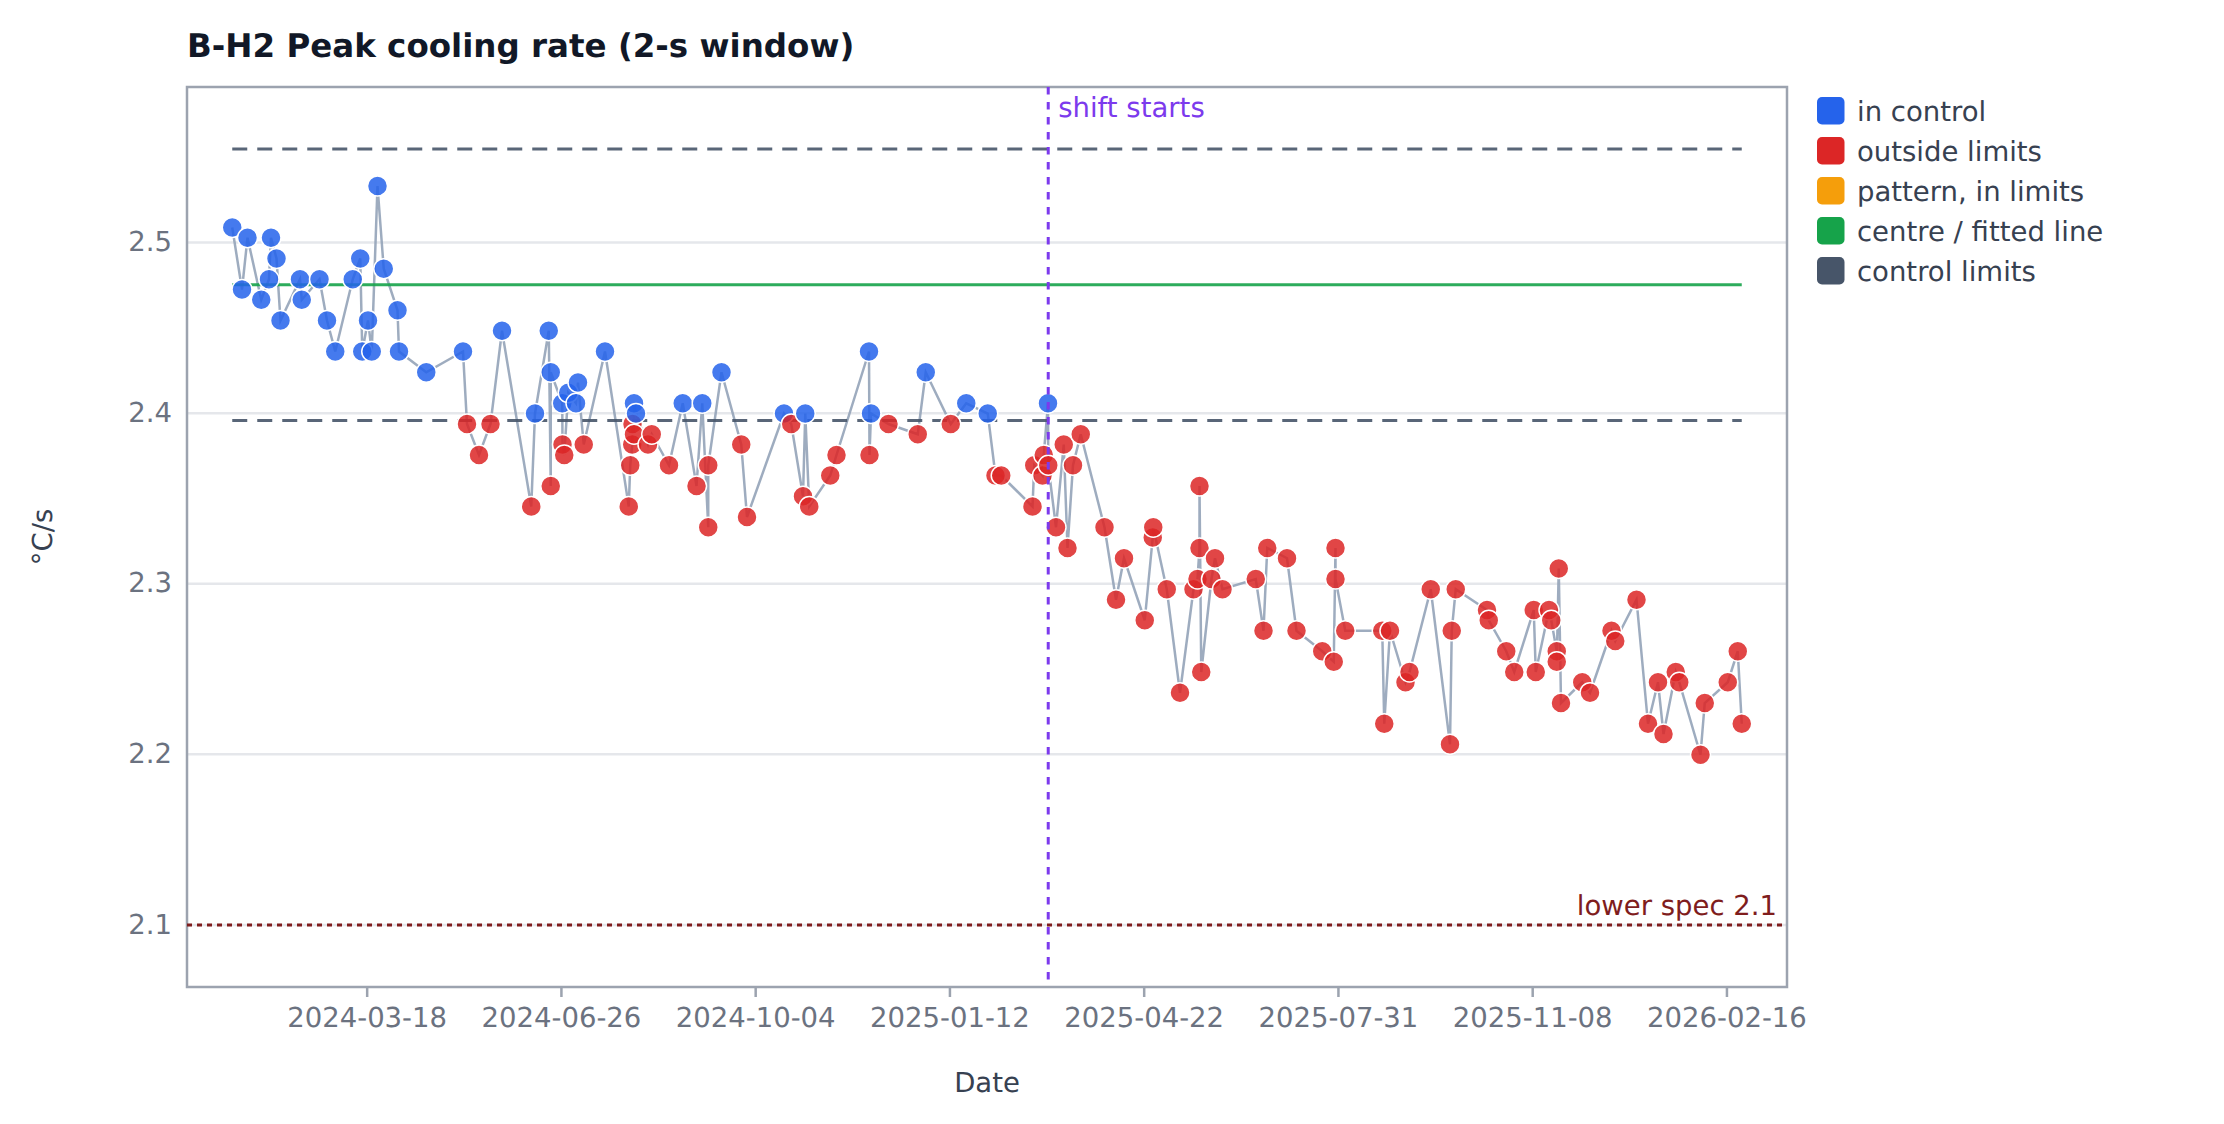
\includegraphics[width=\linewidth]{fig/cc_cool_rate_before.png}\caption{fixed Phase-I fit}\label{fig:cool_before}\end{subfigure}\hfill
\begin{subfigure}{0.49\linewidth}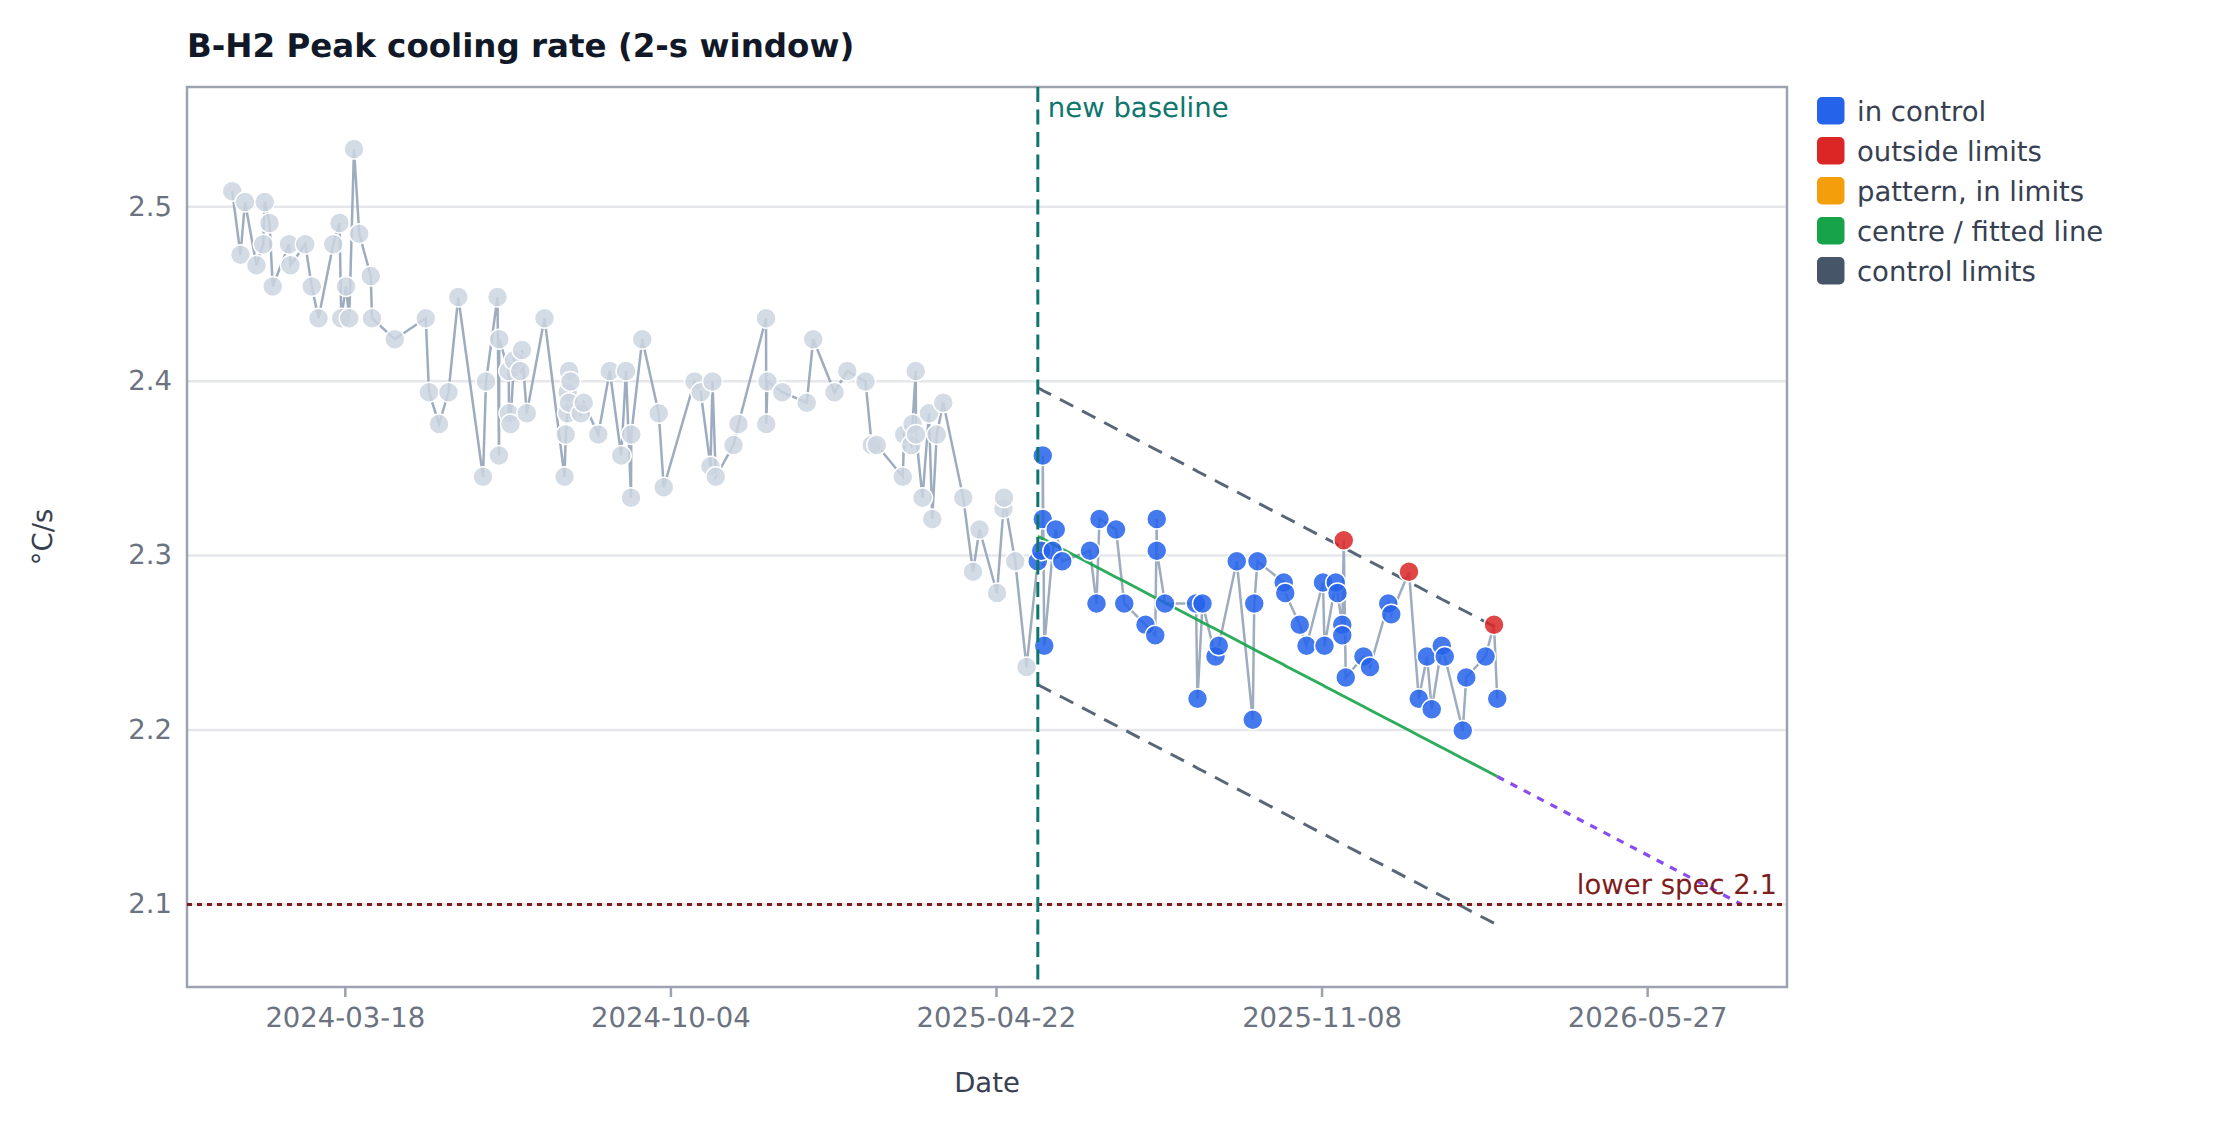
\includegraphics[width=\linewidth]{fig/cc_cool_rate_rebaseline.png}\caption{baseline from the service date}\label{fig:cool_rebase}\end{subfigure}
\caption{\synthtag Trend chart, LC-DEMO-01, B-H2 peak cooling rate against date. (a) The baseline precedes the planted service step.
(b) With \emph{Baseline starts on} = 2025-05-12 the earlier runs are grey, a green marker shows the new baseline and the
fit uses the configured Phase-I runs after service. Forecasts depend on this selection and are illustrative.}\label{fig:cool}
\end{figure}

\begin{figure}[htbp]\centering
\begin{subfigure}{0.49\linewidth}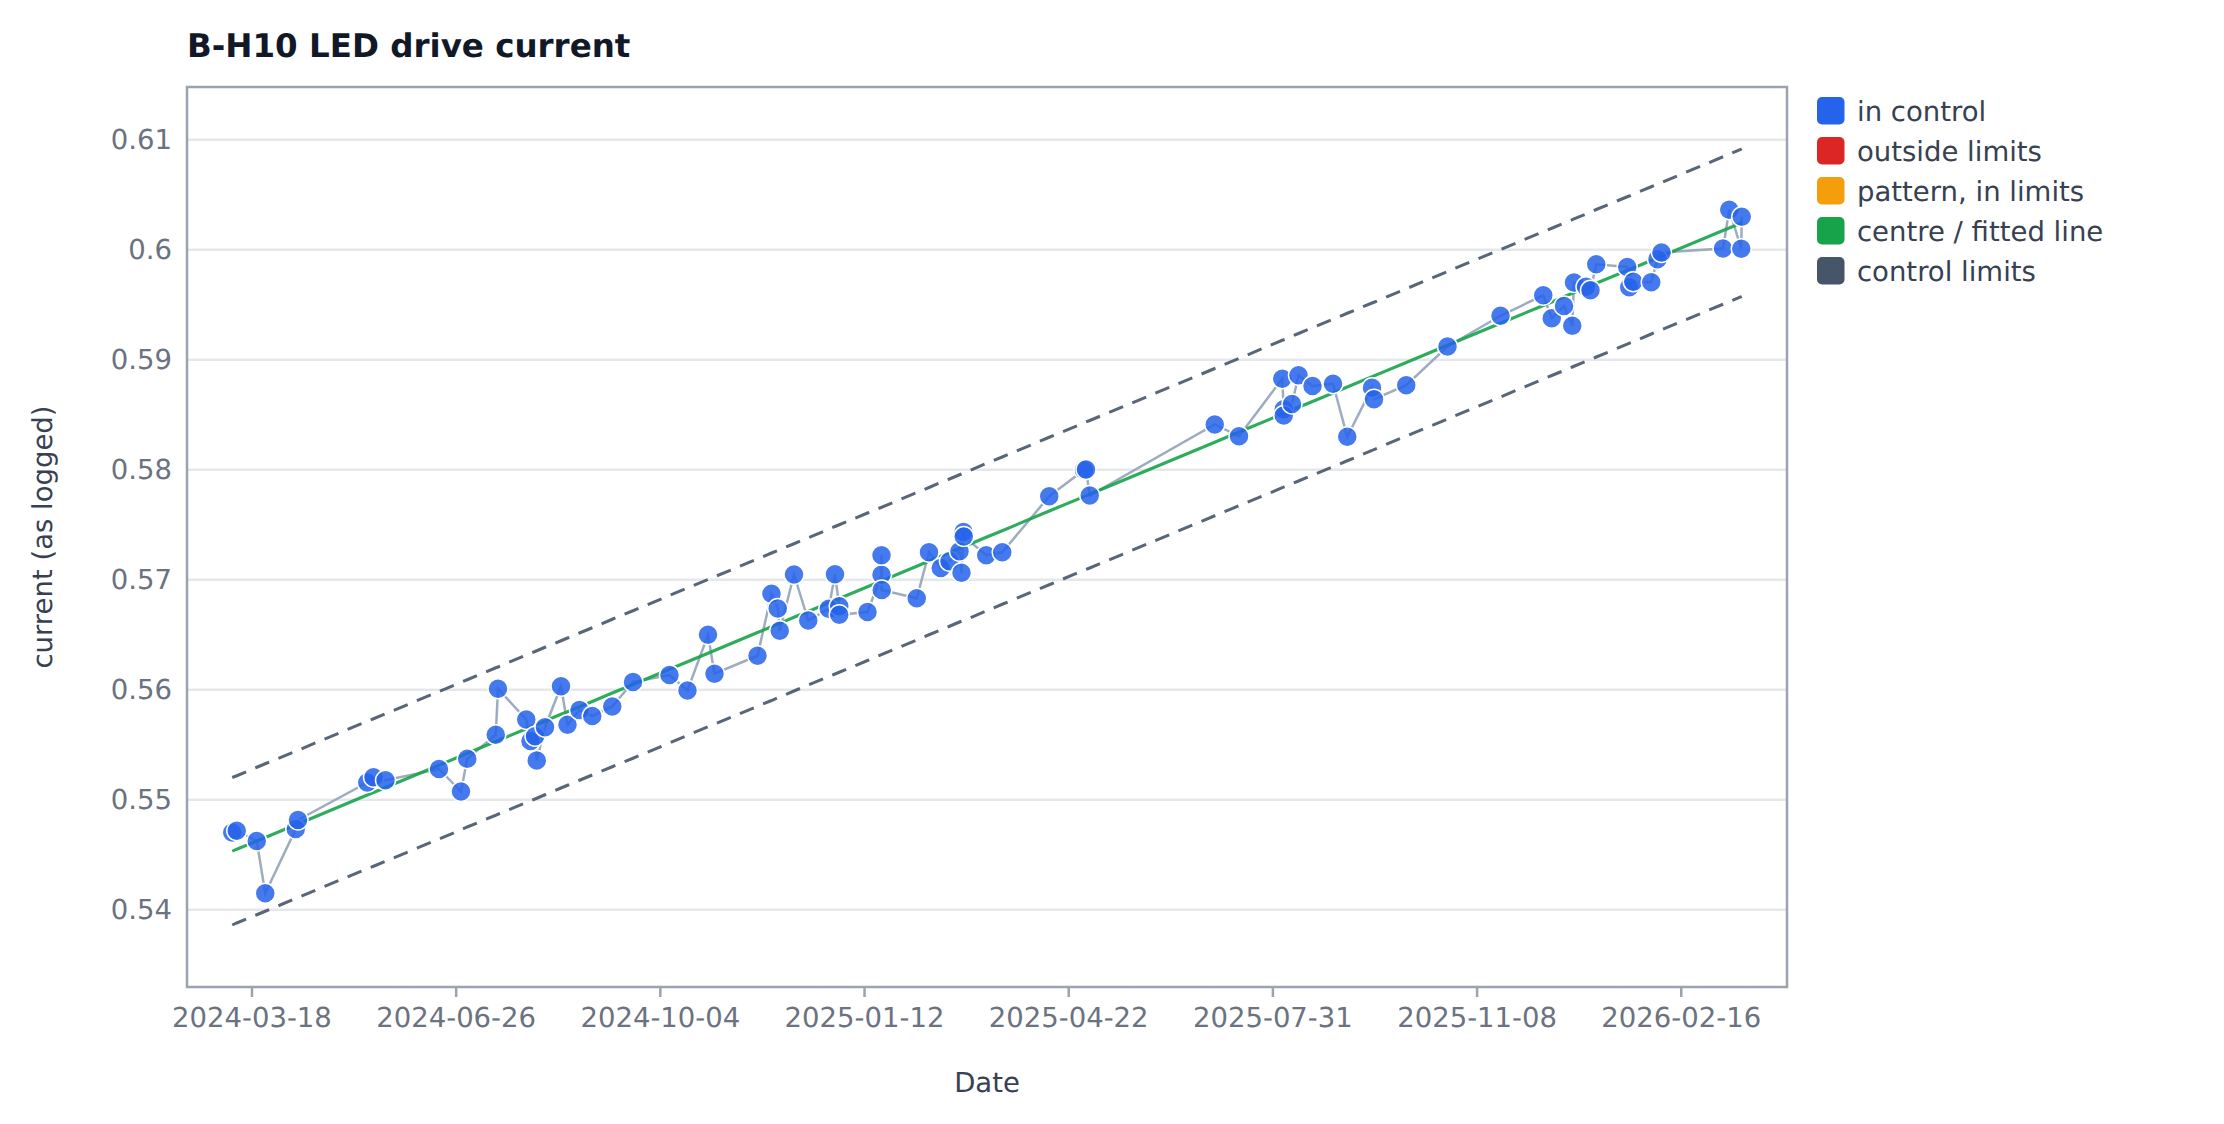
\includegraphics[width=\linewidth]{fig/cc_led_current_trend.png}\caption{B-H10 LED drive current}\end{subfigure}\hfill
\begin{subfigure}{0.49\linewidth}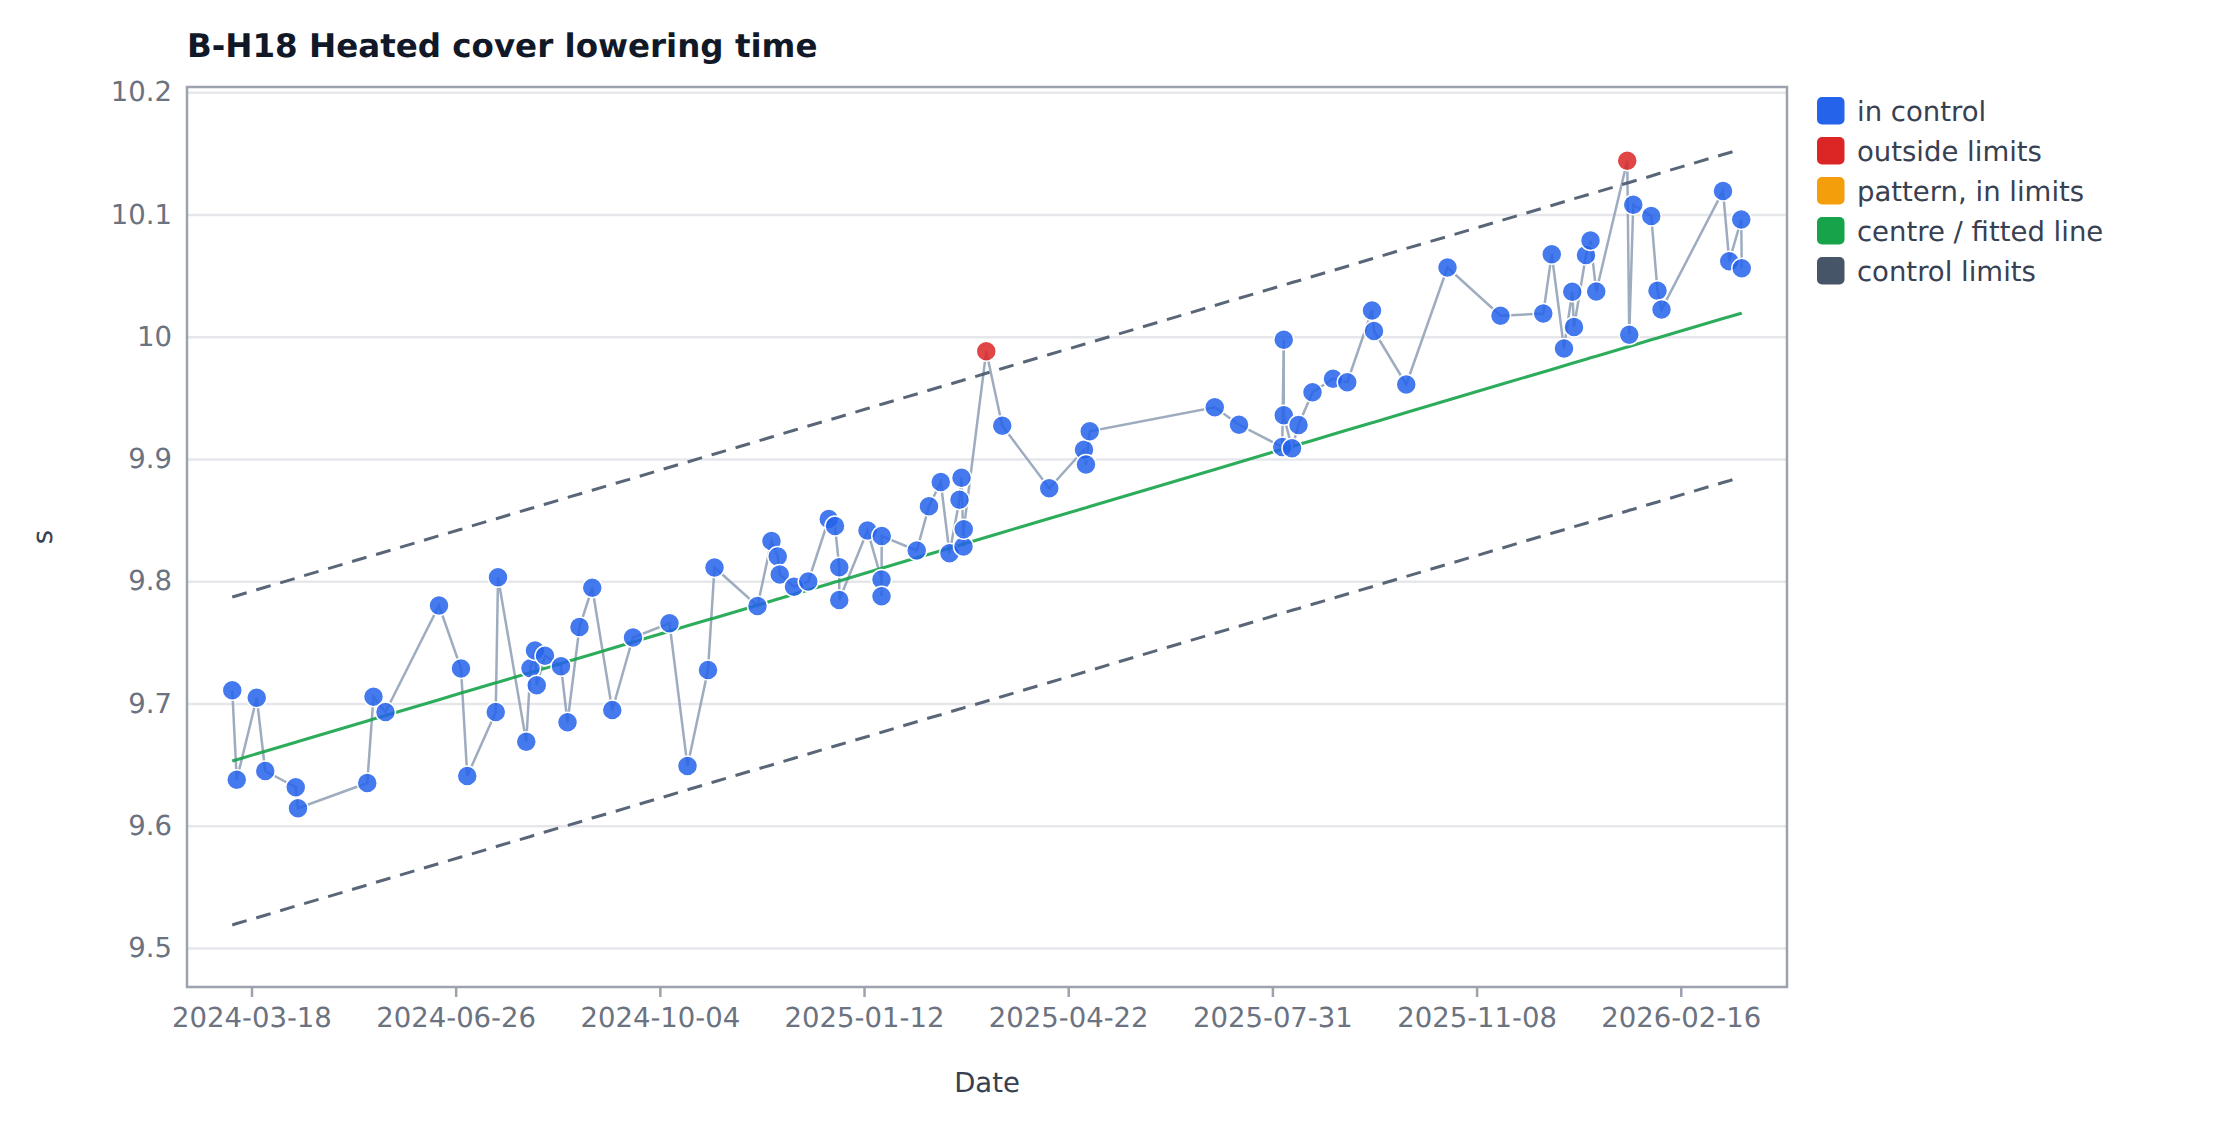
\includegraphics[width=\linewidth]{fig/cc_cover_down_trend.png}\caption{B-H18 heated cover lowering time}\end{subfigure}
\caption{\synthtag Trend charts, QS-DEMO-A: LED drive current and cover-motion time rise by construction. Departures from the fitted band prompt investigation; they do not establish a component failure.}\label{fig:qs_trends}
\end{figure}

\fig[0.9]{cc_heat_rate.png}{Trend chart, LC-DEMO-01, B-H1 peak heating rate against date. The baseline slope is not significant, so the centre line is flat; the planted service step is reported as a sustained shift (Figure~\ref{fig:shift}).}{heat}

\subsection{Sustained shifts and the proposed re-baseline}\label{sec:shift}
After a service, a firmware change or a block exchange the process moves to a new level; every later run then sits outside the
old limits and the chart would stay red indefinitely. \texttt{ccShift()} recognises this pattern — eight consecutive runs
outside on the same side and at least 70\,\% of the later runs on that side — and reports it as one finding: the date it
started, the level before and after, the number of runs since, and whether the new level is still inside the specification.
A button offers that date as the new \emph{baseline start}; nothing is re-baselined automatically, and the specification test
is independent of the control limits.

\par\medskip\noindent{\small\textbf{Listing}~\texttt{ccShift()}\hfill\textcolor{gray}{HTML lines 6074--6085}}\par\nopagebreak
\lstinputlisting[style=vstyle,language=JavaScript,firstnumber=6074]{code/ccShift.js}



\begin{figure}[htbp]\centering
\begin{subfigure}{0.49\linewidth}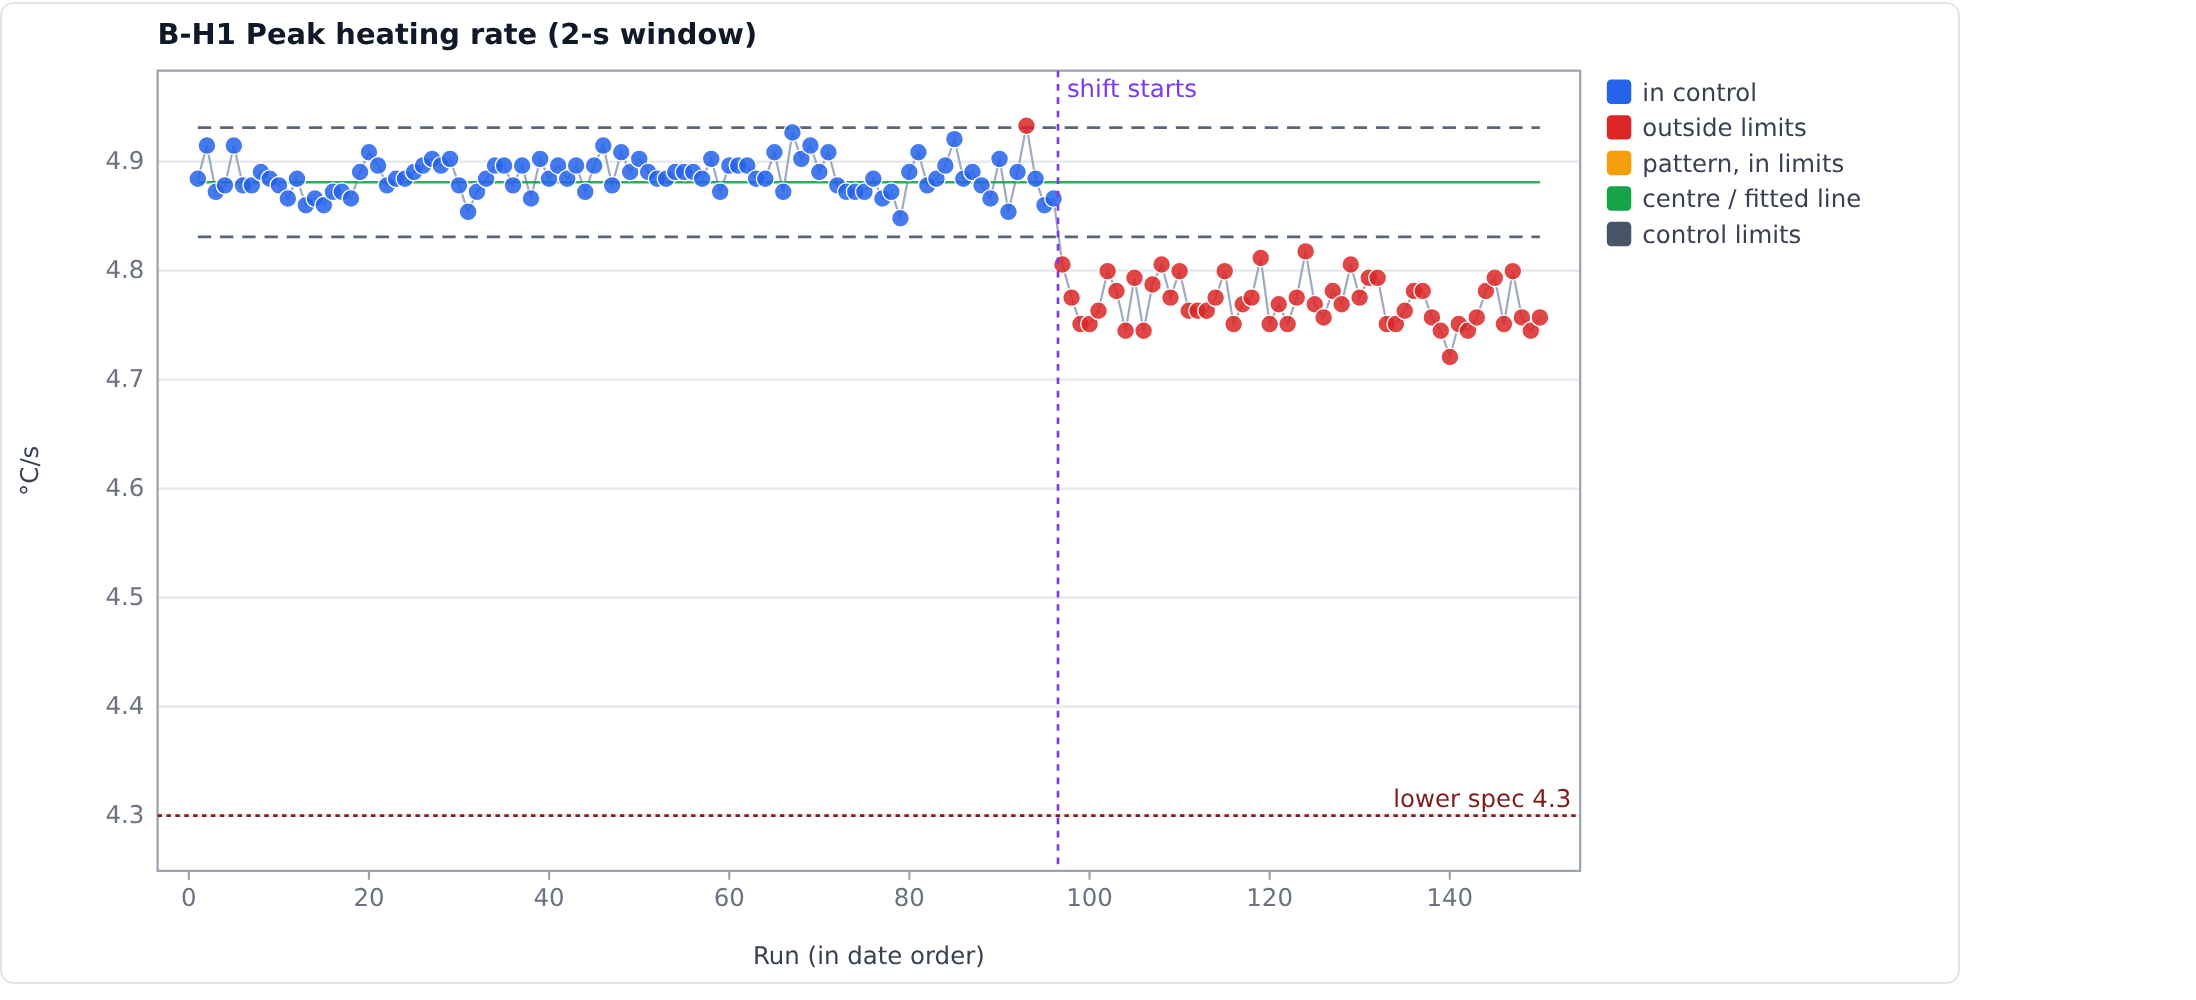
\includegraphics[width=\linewidth]{fig/cc_shift_heat_rate.png}\caption{shift detected, old baseline}\label{fig:shift_a}\end{subfigure}\hfill
\begin{subfigure}{0.49\linewidth}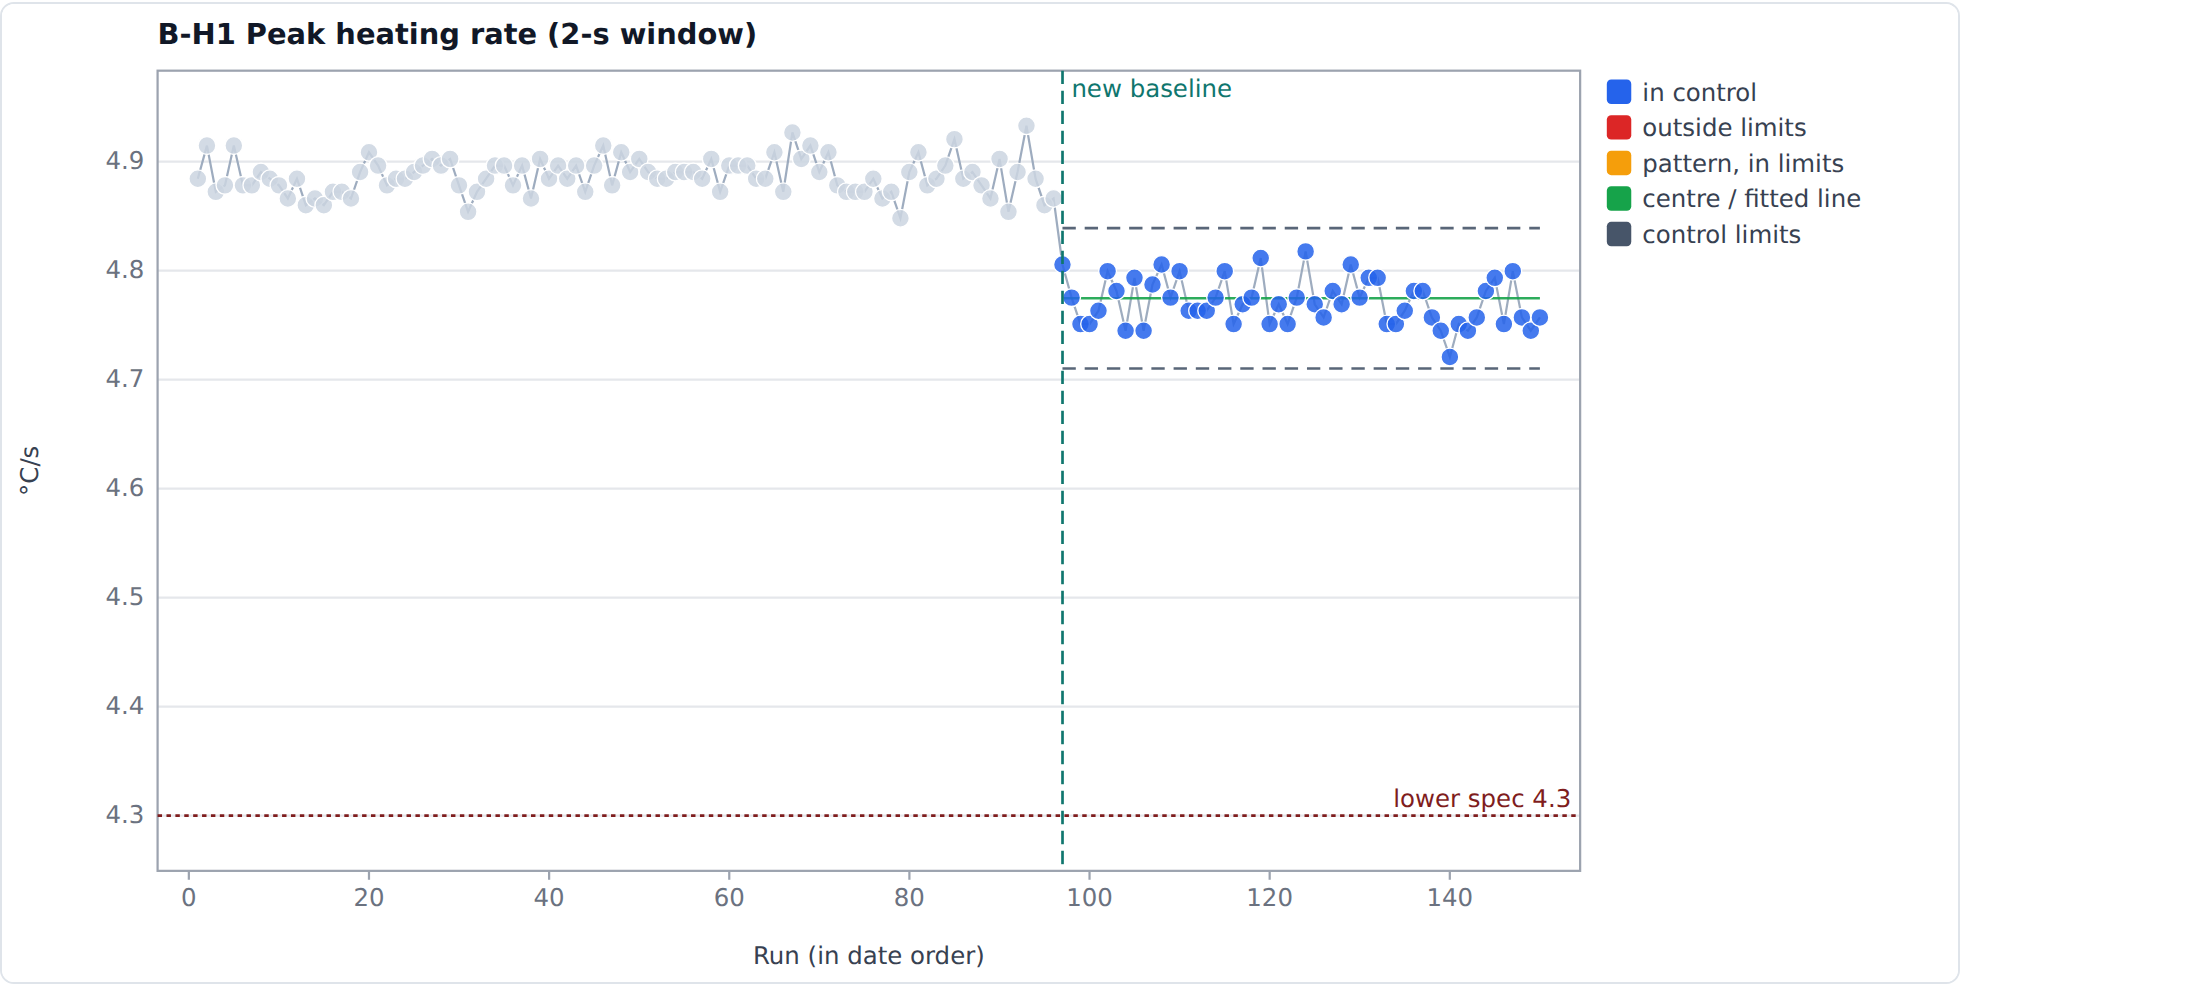
\includegraphics[width=\linewidth]{fig/cc_shift_heat_rate_rebased.png}\caption{after accepting the new baseline}\label{fig:shift_b}\end{subfigure}
\caption{\synthtag B-H1 peak heating rate, LC-DEMO-01, with the planted synthetic service step. (a) the shift is marked and
reported (4.88 $\to$ 4.77\,°C/s, still inside the 4.3\,°C/s specification); (b) with the baseline start set to that date the
earlier runs are grey and the limits describe the current level.}\label{fig:shift}
\end{figure}
\readingnote{A shift is a question about a cause, not a verdict on conformity: check the service record before accepting the
new baseline, and keep the specification comparison separate.}

\subsection{Three-way X̄–S chart}
For many readings per run (45 readings of the block temperature at the moment of reading, or all images of a run) the mean chart uses
\[ \bar{\bar x}\pm\max\!\Big(A_3(n)\,\bar S,\ 3\,\frac{\overline{MR}_{\bar x}}{1.128}\Big),\qquad \text{S chart: } B_4(n)\,\bar S,\quad c_4=\frac{4(n-1)}{4n-3}, \]
the three-way chart of Wheeler: with within-run limits alone ($A_3\bar S$) almost every run would alarm, because the run-to-run
variation is much larger than the variation inside a run.
\par\medskip\noindent{\small\textbf{Listing}~\texttt{ccXbarS()}\hfill\textcolor{gray}{HTML lines 6223--6234}}\par\nopagebreak
\lstinputlisting[style=vstyle,language=JavaScript,firstnumber=6223]{code/ccXbarS.js}


\fig[0.8]{cc_hold_temp_xbars.png}{X̄–S chart, LC-DEMO-01, B-H4 temperature at the moment of reading: the planted recalibration moves the offset from $-0.50$ to about $-0.40$\,°C; the within-run spread (S chart) stays unchanged.}{hold}

\subsection{Attribute charts: p, u, c}
\[ p:\ \bar p\pm3\sqrt{\bar p(1-\bar p)/n_i},\qquad u:\ \bar u\pm3\sqrt{\bar u/e_i},\qquad c:\ \bar c\pm3\sqrt{\bar c}. \]
\par\medskip\noindent{\small\textbf{Listing}~\texttt{ccP()}\hfill\textcolor{gray}{HTML lines 6209--6214}}\par\nopagebreak
\lstinputlisting[style=vstyle,language=JavaScript,firstnumber=6209]{code/ccP.js}


\par\medskip\noindent{\small\textbf{Listing}~\texttt{ccU()}\hfill\textcolor{gray}{HTML lines 6215--6218}}\par\nopagebreak
\lstinputlisting[style=vstyle,language=JavaScript,firstnumber=6215]{code/ccU.js}


\par\medskip\noindent{\small\textbf{Listing}~\texttt{ccC()}\hfill\textcolor{gray}{HTML lines 6219--6222}}\par\nopagebreak
\lstinputlisting[style=vstyle,language=JavaScript,firstnumber=6219]{code/ccC.js}


\fig[0.9]{cc_ntc_p.png}{p chart, B-M5 share of NTC / blank wells with a Cq. The limits widen and narrow with the number of NTC wells per run.}{ntcp}
\fig[0.9]{cc_copied.png}{c chart, B-O11 copied-data events: the planted copied curve in run 013 is the only event.}{copied}

\subsection{Funnel plot by operator}
Each operator is one point: rate against workload $n$, with 95\,\% and 99.8\,\% limits $p_0\pm1.96$ and $\pm3.09\sqrt{p_0(1-p_0)/n}$.
It compares people with different workloads fairly and is meant for training, not ranking.
\par\medskip\noindent{\small\textbf{Listing}~\texttt{ccFunnel()}\hfill\textcolor{gray}{HTML lines 6235--6241}}\par\nopagebreak
\lstinputlisting[style=vstyle,language=JavaScript,firstnumber=6235]{code/ccFunnel.js}


\fig[0.85]{cc_ntc_funnel.png}{Funnel plot, B-O5 selected negative-control stage by operator. Workload is shown, but assay and batch confounding are not adjusted.}{funnel}
\fig[0.9]{cc_rep_sd.png}{I chart coloured by operator, B-O1 replicate precision (pooled SD of replicates with Cq $<30$): the points of Analyst B sit higher.}{repsd}

\subsection{Transition times, lamp, exposure and processing delay}
\begin{figure}[htbp]\centering
\begin{subfigure}{0.49\linewidth}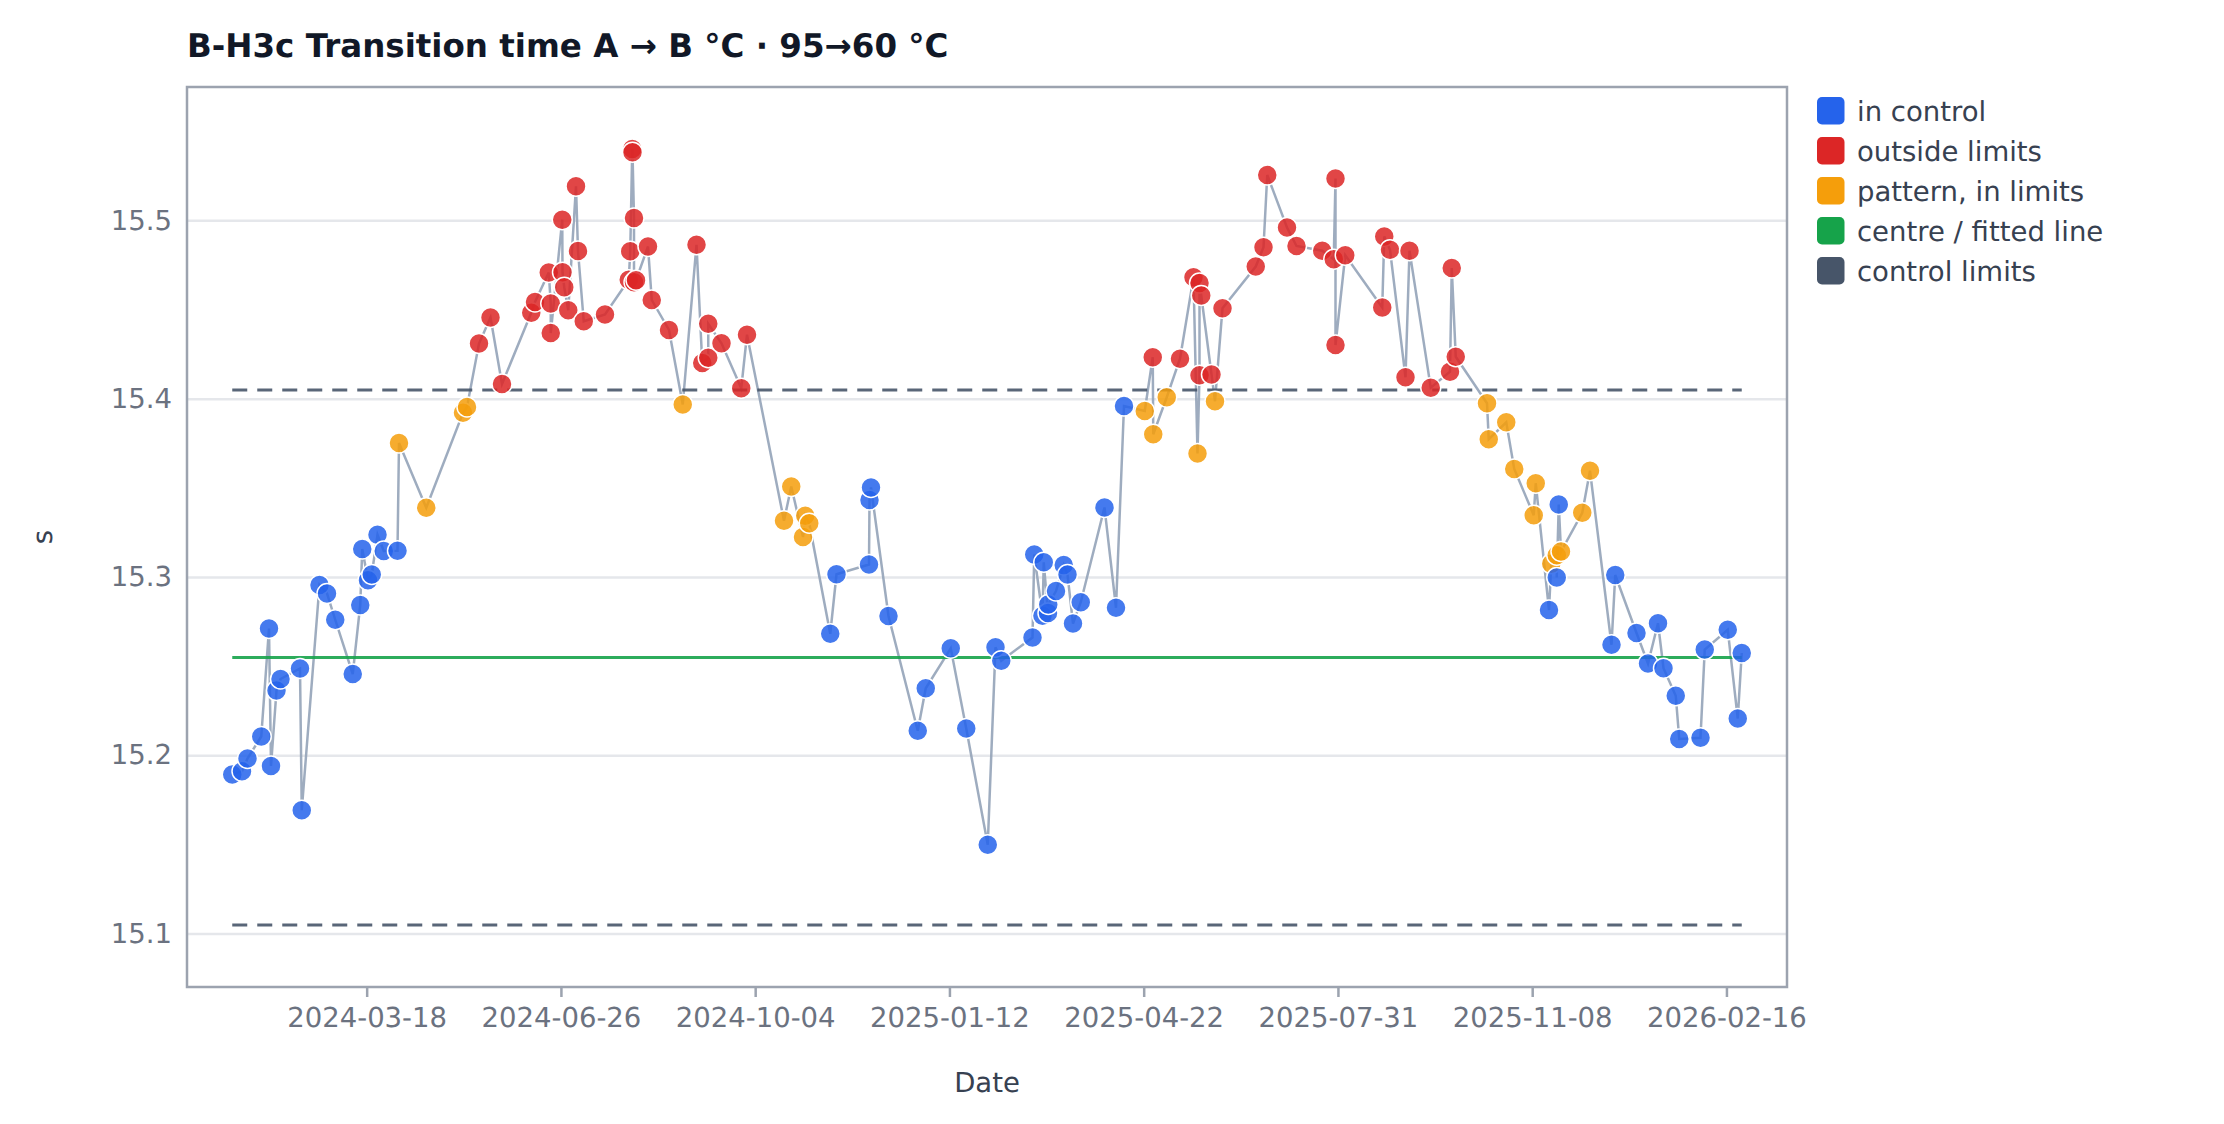
\includegraphics[width=\linewidth]{fig/cc_transition_95_60.png}\caption{95 $\to$ 60 °C}\end{subfigure}\hfill
\begin{subfigure}{0.49\linewidth}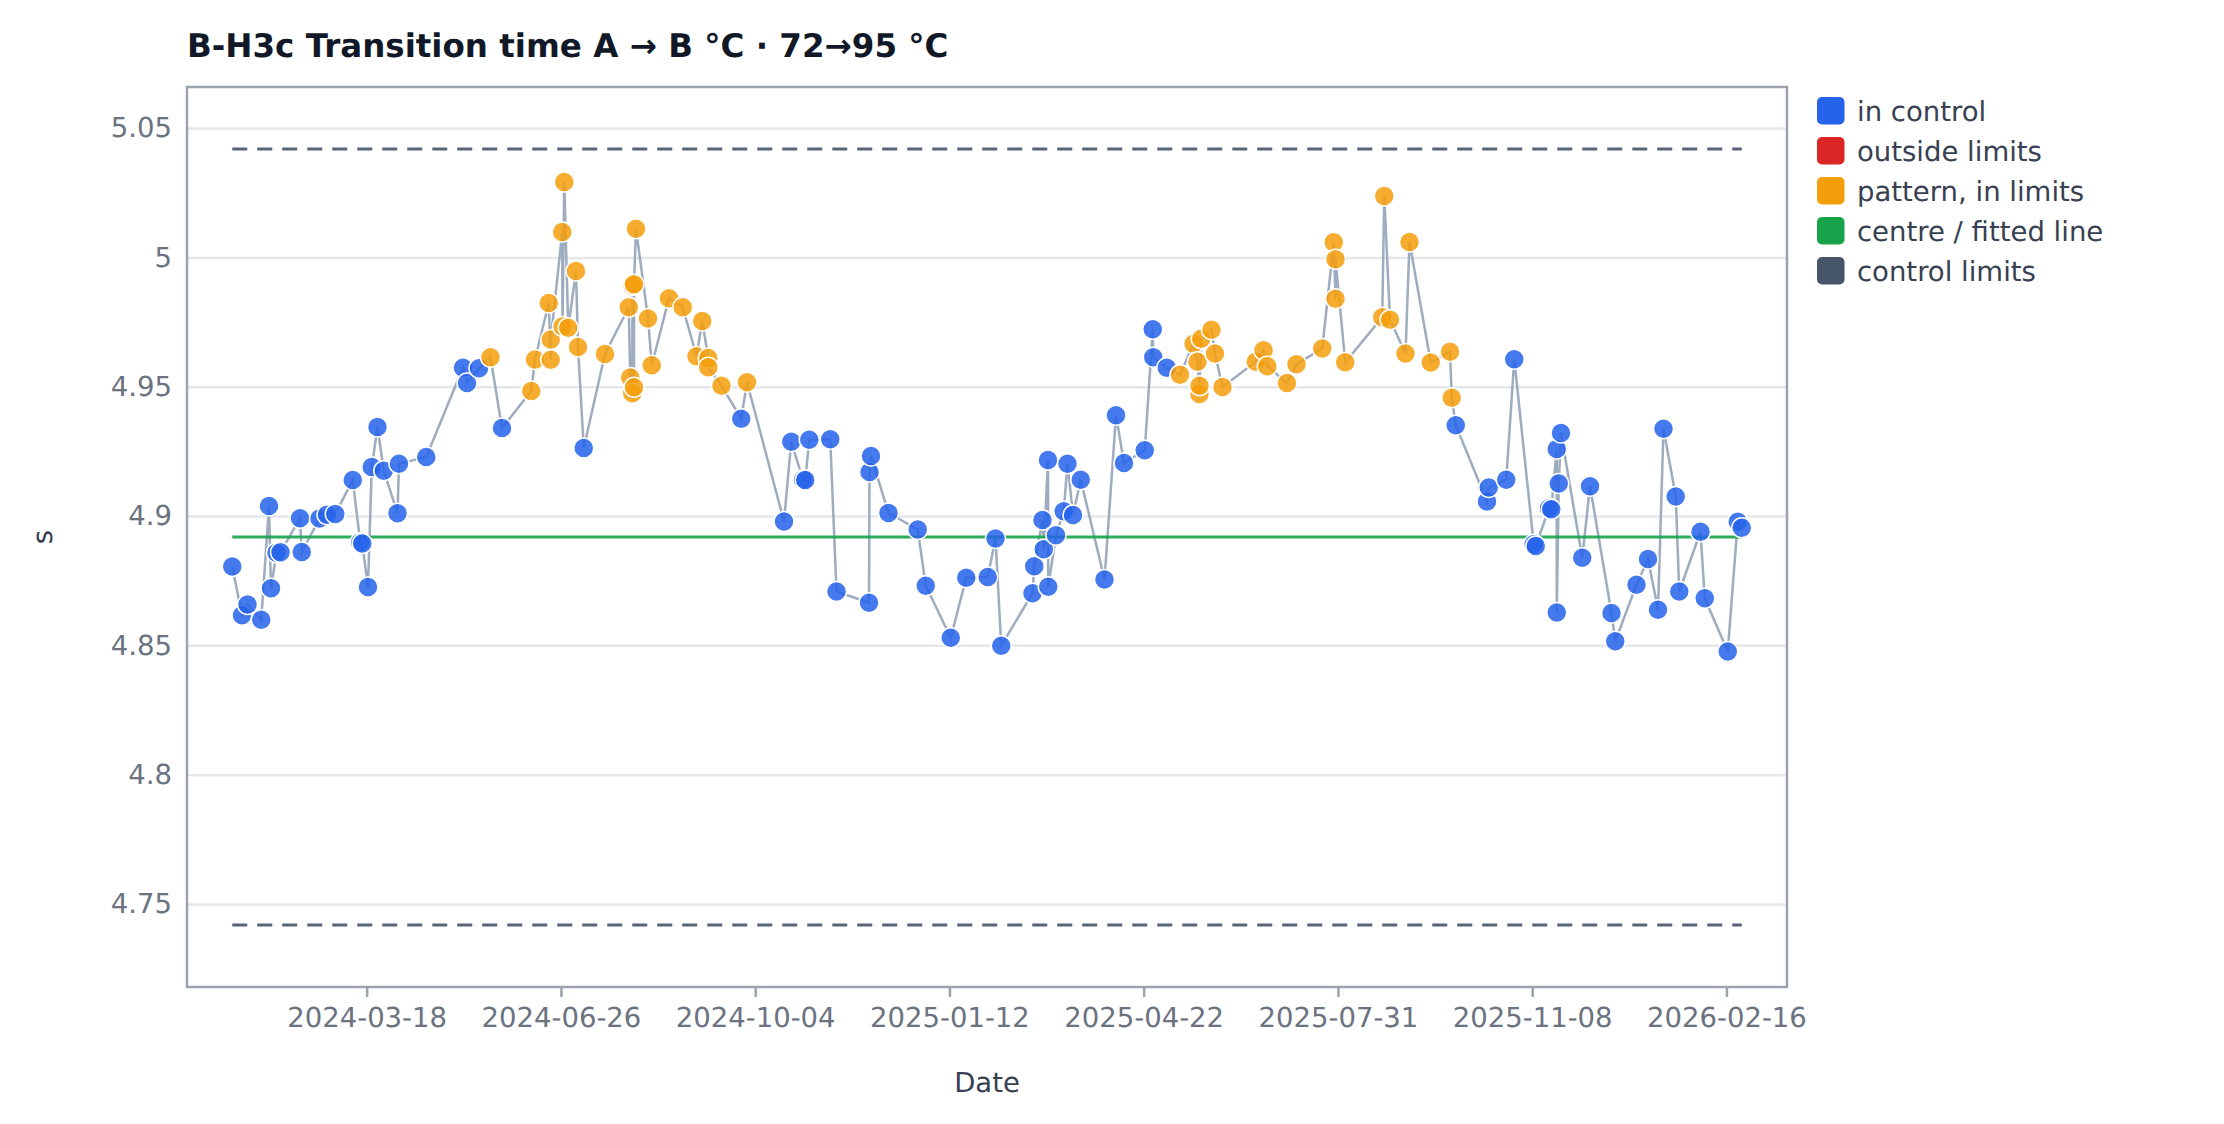
\includegraphics[width=\linewidth]{fig/cc_transition_72_95.png}\caption{72 $\to$ 95 °C}\end{subfigure}
\caption{\synthtag B-H3c transition times, LC-DEMO-01, against date. The history shows the planted seasonality (95\,$\to$\,60 longer in summer, 72\,$\to$\,95 longer in winter); in the most recent runs the cooling capacity drops below what the program asks for and 95\,$\to$\,60\,°C lengthens run after run.}\label{fig:trans}
\end{figure}
\fig[0.85]{cc_qs_transition_60_95.png}{B-H3c for QS-DEMO-A, 60 $\to$ 95 °C (1-s modelled sample temperature, interpolated crossings).}{qs_trans}
\begin{figure}[htbp]\centering
\begin{subfigure}{0.49\linewidth}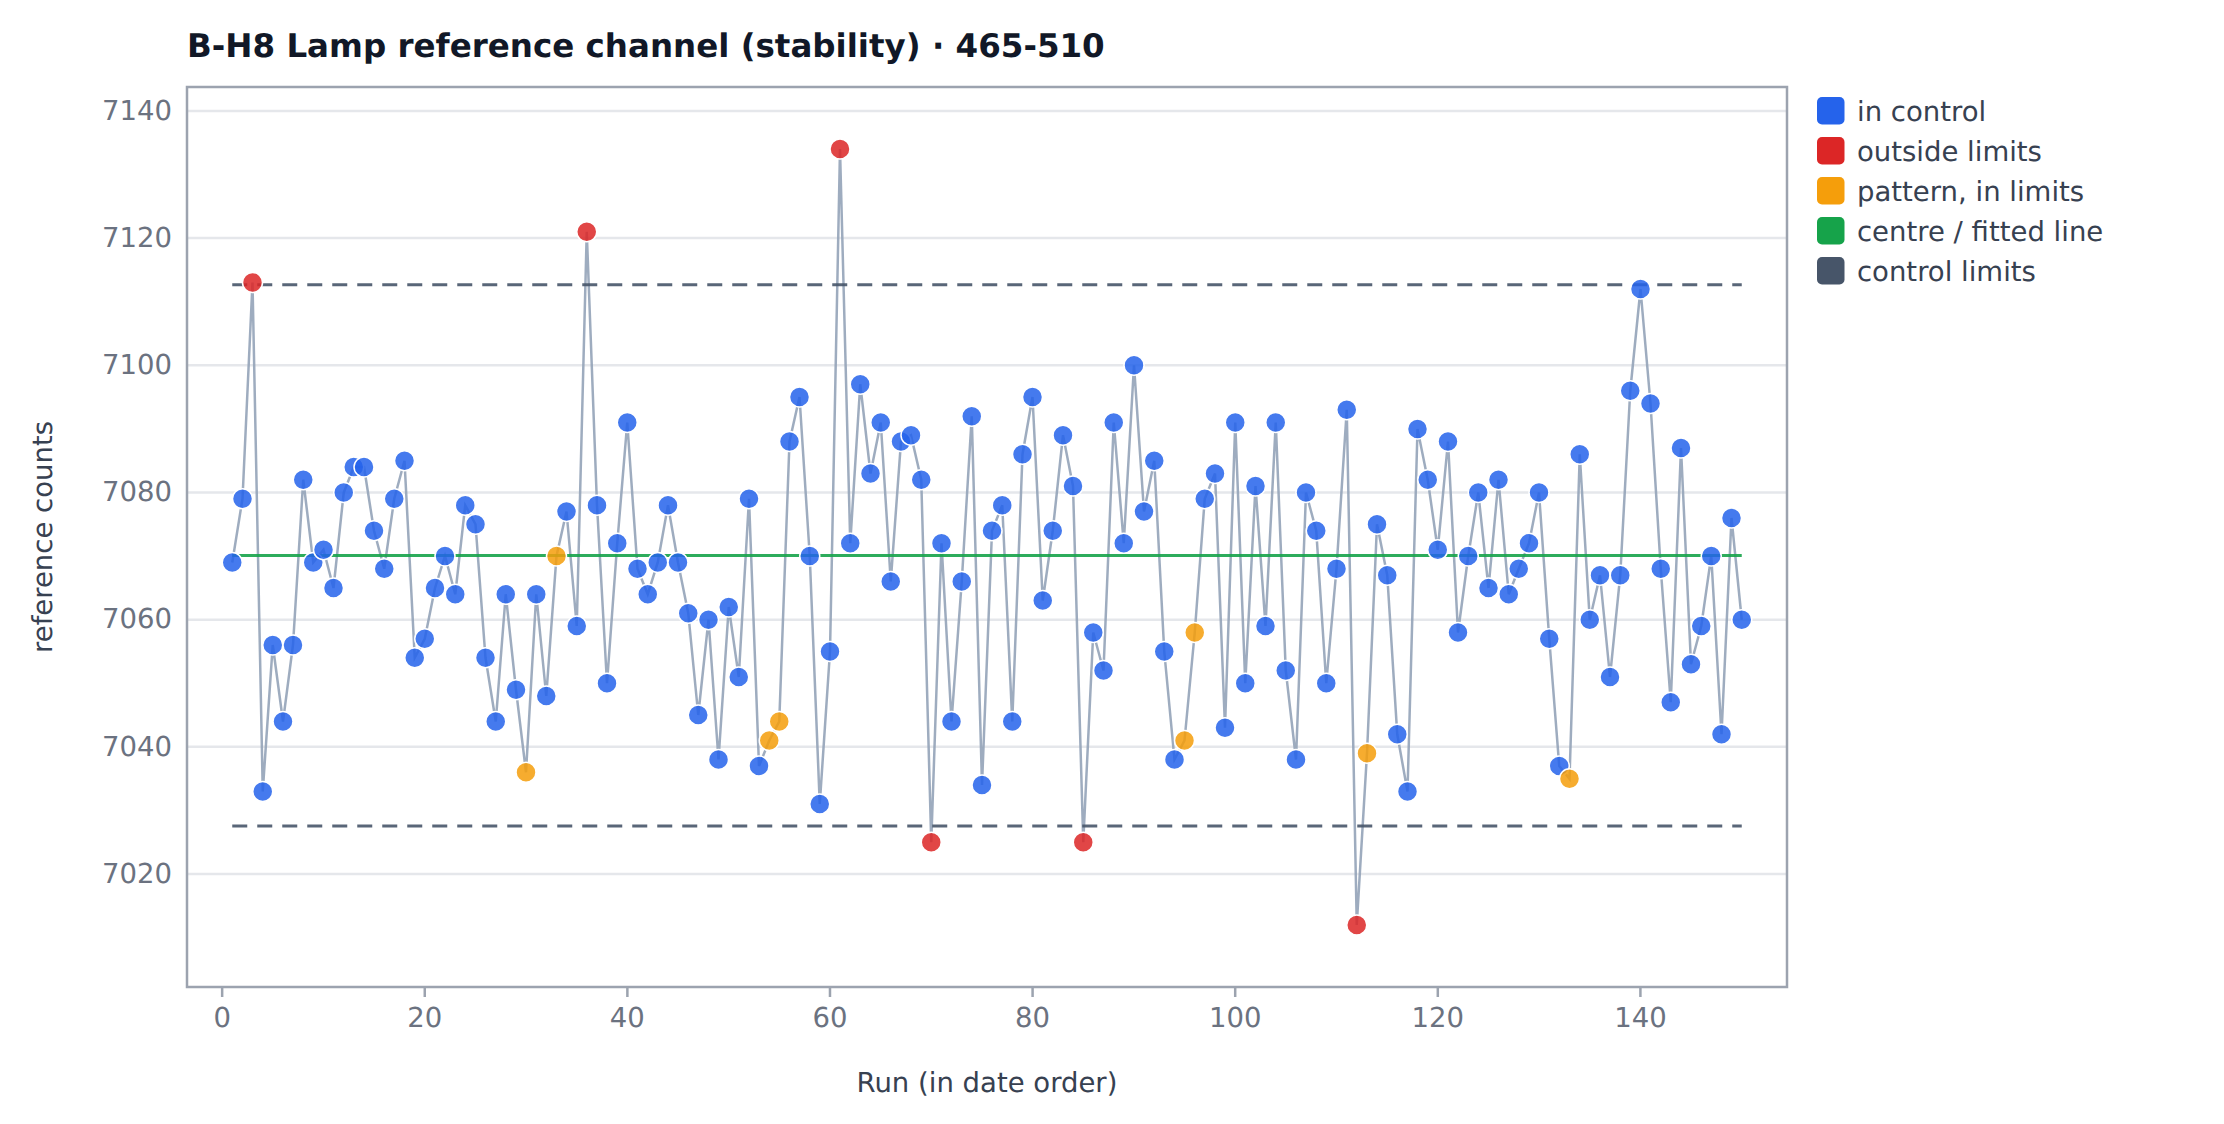
\includegraphics[width=\linewidth]{fig/cc_lamp_ref.png}\caption{B-H8 lamp reference channel 465-510}\end{subfigure}\hfill
\begin{subfigure}{0.49\linewidth}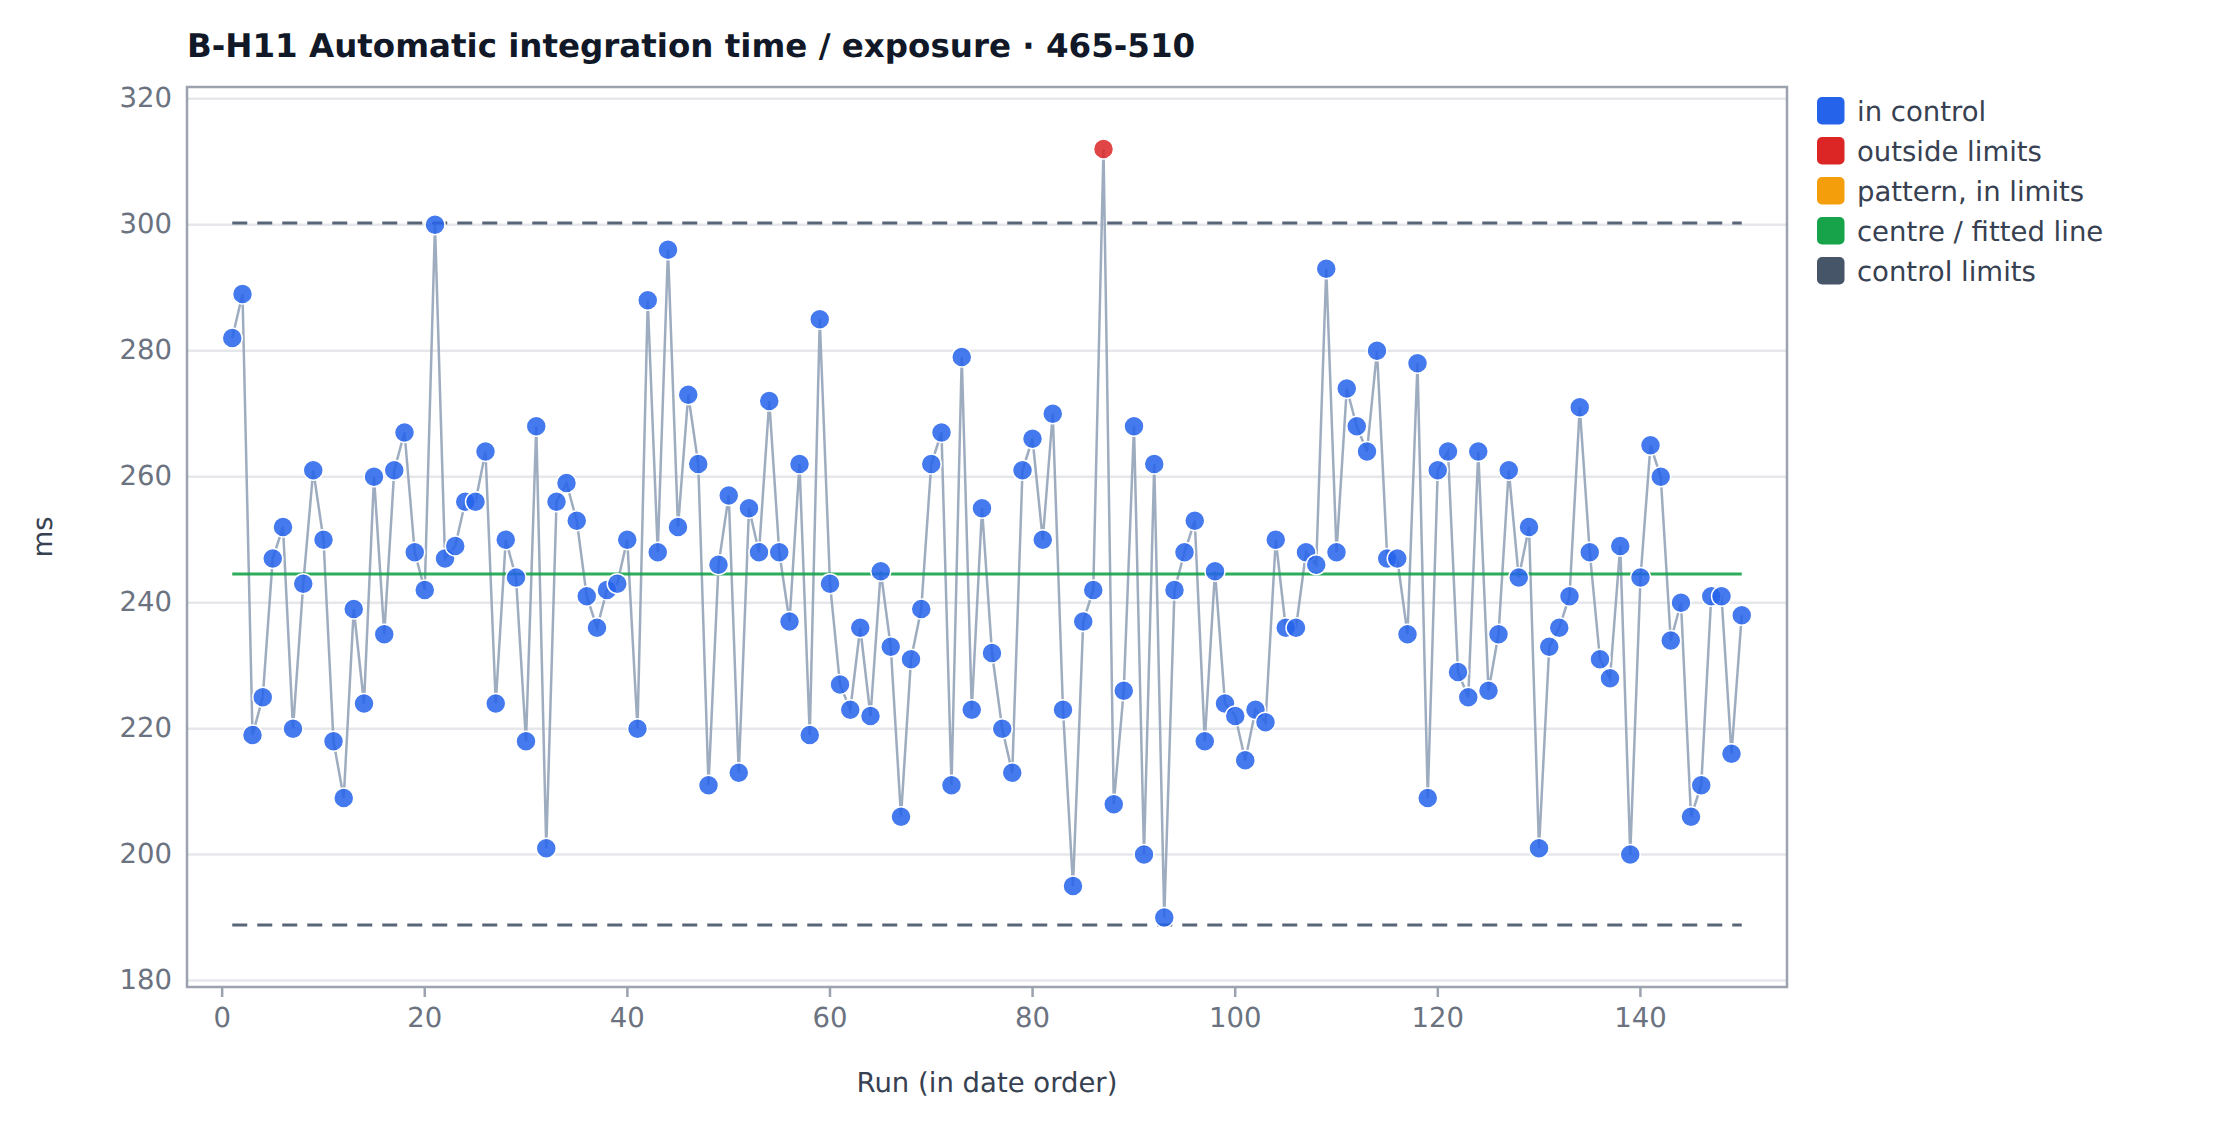
\includegraphics[width=\linewidth]{fig/cc_exposure.png}\caption{B-H11 automatic integration time 465-510}\end{subfigure}
\caption{\synthtag .ixo instrument optics: the lamp reference is regulated and stays flat; the exposure rises slowly as the synthetic optics lose light.}\label{fig:optics}
\end{figure}
\fig[0.9]{cc_edit_delay.png}{A-S4 run end $\to$ last change (log$_{10}$ hours): the planted late change of run 018 (410\,h) stands out.}{editdelay}
\fig[0.9]{cc_cmd_rt.png}{B-S1 reply time of the .eds instrument's embedded computer to the PC software (95th percentile per run).}{cmdrt}

\section{From chart definition to status}
\texttt{ccCompute()} selects the rows that carry the metric, applies the baseline date and the resolution floor, calls the
chart function and adds the specification limits; \texttt{ccStatus()} turns the result into the tile status.

\par\medskip\noindent{\small\textbf{Listing}~\texttt{CC\_GROUPS and the first entries of CC\_CHARTS}\hfill\textcolor{gray}{HTML lines 5940--5954}}\par\nopagebreak
\lstinputlisting[style=vstyle,language=JavaScript,firstnumber=5940]{code/cc_charts_head.js}


\par\medskip\noindent{\small\textbf{Listing}~\texttt{CC\_CHARTS entry B-H3c (transition time)}\hfill\textcolor{gray}{HTML lines 5963--5966}}\par\nopagebreak
\lstinputlisting[style=vstyle,language=JavaScript,firstnumber=5963]{code/cc_transition_def.js}


\par\medskip\noindent{\small\textbf{Listing}~\texttt{ccSpec()}\hfill\textcolor{gray}{HTML lines 6372--6377}}\par\nopagebreak
\lstinputlisting[style=vstyle,language=JavaScript,firstnumber=6372]{code/ccSpec.js}


\par\medskip\noindent{\small\textbf{Listing}~\texttt{ccXAxis()}\hfill\textcolor{gray}{HTML lines 6365--6371}}\par\nopagebreak
\lstinputlisting[style=vstyle,language=JavaScript,firstnumber=6365]{code/ccXAxis.js}


\par\medskip\noindent{\small\textbf{Listing}~\texttt{ccCompute()}\hfill\textcolor{gray}{HTML lines 6378--6428}}\par\nopagebreak
\lstinputlisting[style=vstyle,language=JavaScript,firstnumber=6378]{code/ccCompute.js}


\par\medskip\noindent{\small\textbf{Listing}~\texttt{ccStatus()}\hfill\textcolor{gray}{HTML lines 6444--6469}}\par\nopagebreak
\lstinputlisting[style=vstyle,language=JavaScript,firstnumber=6444]{code/ccStatus.js}



\section{The chart page and its settings}
\figui[0.9]{ui_chart_page_cool.png}{Chart page of B-H2: chart, status line with the forecast, \emph{How to read it}, the meaning of a result below and above the limits, and the settings of this chart.}{ui_chart_page}

Every chart has two texts that say what a result \textbf{below the lower limit} and \textbf{above the upper limit} means and
what to check first; the alarm table marks each alarm as ▼ below or ▲ above. Control-chart alarms stay in this panel so
quality review is reserved for file, timeline, result and interpretation evidence.

\figui{ui_limit_texts.png}{The two interpretation boxes of a chart page.}{ui_limits}
\par\medskip\noindent{\small\textbf{Listing}~\texttt{CC\_LIMIT\_TEXT — first entries (one per chart)}\hfill\textcolor{gray}{HTML lines 6244--6249}}\par\nopagebreak
\lstinputlisting[style=vstyle,language=JavaScript,firstnumber=6244]{code/cc_limit_text.js}


\par\medskip\noindent{\small\textbf{Listing}~\texttt{ccAlarmDir()}\hfill\textcolor{gray}{HTML lines 6308--6314}}\par\nopagebreak
\lstinputlisting[style=vstyle,language=JavaScript,firstnumber=6308]{code/ccAlarmDir.js}



The settings are stored in the SOP profile under \texttt{controlCharts}, so they are versioned and covered by the profile's
SHA-256 like any other rule (Chapter~\ref{ch:sop}).

\figui{ui_chart_settings.png}{Settings of a chart: alarm action, baseline runs, baseline start date (after a repair or service), specification limits, warning horizon and how the wear line is fitted.}{ui_settings}
\par\medskip\noindent{\small\textbf{Listing}~\texttt{CC\_DEFAULT\_CFG()}\hfill\textcolor{gray}{HTML lines 6131--6132}}\par\nopagebreak
\lstinputlisting[style=vstyle,language=JavaScript,firstnumber=6131]{code/CC_DEFAULT_CFG.js}


\par\medskip\noindent{\small\textbf{Listing}~\texttt{ccCfg()}\hfill\textcolor{gray}{HTML lines 6136--6137}}\par\nopagebreak
\lstinputlisting[style=vstyle,language=JavaScript,firstnumber=6136]{code/ccCfg.js}


\par\medskip\noindent{\small\textbf{Listing}~\texttt{ccSetCfg()}\hfill\textcolor{gray}{HTML lines 6138--6139}}\par\nopagebreak
\lstinputlisting[style=vstyle,language=JavaScript,firstnumber=6138]{code/ccSetCfg.js}



\section{Alarms in the control panel}
The panel summary counts alarm points for the selected instrument and lists them by chart. These are monitoring signals,
not duplicate forensic findings. The chart CSV and SVG exports retain the full alarm detail.
\par\medskip\noindent{\small\textbf{Listing}~\texttt{ccEvents()}\hfill\textcolor{gray}{HTML lines 6777--6788}}\par\nopagebreak
\lstinputlisting[style=vstyle,language=JavaScript,firstnumber=6777]{code/ccEvents.js}



\section{All control charts of all instruments in one ZIP}
The button \emph{All control charts, all instruments (ZIP)} writes, for every instrument, every chart (and every channel,
target or transition) as SVG and CSV (optionally PNG), a summary table and the instrument history:

\begin{lstlisting}[style=vstyle,language=text, numbers=left,firstnumber=1]
control_charts_all_instruments_<date>.zip
├── README.txt            profile, SHA-256, protocol filter, one line per instrument
├── sop_profile.json
├── LC_LC-DEMO-01/        86 files
│   ├── 00_summary.csv    status of every chart on the latest run
│   ├── B-H2_cool_rate.svg / .csv
│   ├── B-H3c_transition_95-to-60.svg / .csv
│   ├── B-H4_hold_temp.svg, B-H4_hold_temp_S-chart.svg, .csv
│   ├── … one file pair per chart and variant
│   └── history.json / history.csv
├── LC_LC-DEMO-02/  QS_QS-DEMO-A/  QS_QS-DEMO-B/
\end{lstlisting}
The synthetic data set gives 407 files in four folders.

{\footnotesize
\begin{longtable}{@{}lllllll@{}}
\toprule \textbf{Column 1} & \textbf{Column 2} & \textbf{Column 3} & \textbf{Column 4} & \textbf{Column 5} & \textbf{Column 6} & \textbf{Column 7} \\\midrule\endfirsthead
\toprule \textbf{Column 1} & \textbf{Column 2} & \textbf{Column 3} & \textbf{Column 4} & \textbf{Column 5} & \textbf{Column 6} & \textbf{Column 7} \\\midrule\endhead
A-H4 & Run duration &  & alarm & 97.597 & 36 & 8 on one side \\\hline
A-M1 & Positive control … & 35S | DEMO LOD 01… & alarm & 32.125 & 19 & 10-x \\\hline
B-H1 & Peak heating rate… &  & alarm & 4.780 & 127 & off the trend lin… \\\hline
B-H2 & Peak cooling rate… &  & alarm & 2.238 & 15 & off the trend lin… \\\hline
B-H3 & Overshoot at the … &  & alarm & 6.100 & 113 & downward shift (C… \\\hline
B-H3b & Settling time at … &  & alarm & 5.330 & 152 & beyond 3σ, 2 of 3… \\\hline
B-H3c & Transition time A… & 95→60 °C & alarm & 15.292 & 124 & beyond 3σ, 2 of 3… \\\hline
B-H3c & Transition time A… & 60→72 °C & alarm & 2.330 & 37 & 8 on one side \\\hline
B-H3c & Transition time A… & 72→95 °C & alarm & 5.797 & 108 & 8 on one side \\\hline
B-H3c & Transition time A… & 72→40 °C & alarm & 13.965 & 27 & 4 of 5 beyond 1σ,… \\\hline
B-H4 & Temperature at th… &  & alarm & -0.412 & 87 & mean beyond limit \\\hline
B-O1 & Replicate precisi… &  & alarm & 0.718 & 33 & beyond 3σ, 2 of 3… \\\hline
\bottomrule
\end{longtable}}


\par\medskip\noindent{\small\textbf{Listing}~\texttt{ccChartRows()}\hfill\textcolor{gray}{HTML lines 6672--6679}}\par\nopagebreak
\lstinputlisting[style=vstyle,language=JavaScript,firstnumber=6672]{code/ccChartRows.js}


\par\medskip\noindent{\small\textbf{Listing}~\texttt{ccZipAll()}\hfill\textcolor{gray}{HTML lines 6689--6737}}\par\nopagebreak
\lstinputlisting[style=vstyle,language=JavaScript,firstnumber=6689]{code/ccZipAll.js}



\figui[0.82]{ui_panel_qsa.png}{Control panel for the synthetic .eds instrument \texttt{QS-DEMO-A}: the .eds instrument-only charts (LED, zones, heat sink, cover, filter wheel, camera, embedded computer, calibrations) appear here.}{ui_panel_qsa}



\chapter{Tab 5 · Graphs}\label{ch:graphs}

\section{How graphs are drawn}
All graphs are SVG drawn by one function, \texttt{svgPlot()}, without any plotting library. The SOP profile supplies the
limits (Cq cut-off, late-signal limit, maximum replicate SD, zone spread), the outcome colours and the labels, so every graph
changes when the profile changes and carries the profile's name, version and SHA-256. Each graph can be saved as SVG or PNG
together with the numbers behind it (CSV); one button saves all graphs of a run and all cross-run graphs as a ZIP.

\par\medskip\noindent{\small\textbf{Listing}~\texttt{svgPlot()}\hfill\textcolor{gray}{HTML lines 4988--5032}}\par\nopagebreak
\lstinputlisting[style=vstyle,language=JavaScript,firstnumber=4988]{code/svgPlot.js}


\par\medskip\noindent{\small\textbf{Listing}~\texttt{niceTicks()}\hfill\textcolor{gray}{HTML lines 4978--4985}}\par\nopagebreak
\lstinputlisting[style=vstyle,language=JavaScript,firstnumber=4978]{code/niceTicks.js}



A graph is one entry of the array \texttt{GRAPHS}: an id, a group, a title, a note and a \texttt{render(c)} function that
returns the SVG and the rows of its CSV.

\par\medskip\noindent{\small\textbf{Listing}~\texttt{GRAPHS entry: amplification curves}\hfill\textcolor{gray}{HTML lines 5079--5097}}\par\nopagebreak
\lstinputlisting[style=vstyle,language=JavaScript,firstnumber=5079]{code/graph_curves.js}


\par\medskip\noindent{\small\textbf{Listing}~\texttt{graphContext()}\hfill\textcolor{gray}{HTML lines 5414--5419}}\par\nopagebreak
\lstinputlisting[style=vstyle,language=JavaScript,firstnumber=5414]{code/graphContext.js}


\par\medskip\noindent{\small\textbf{Listing}~\texttt{graphAllZip()}\hfill\textcolor{gray}{HTML lines 5461--5481}}\par\nopagebreak
\lstinputlisting[style=vstyle,language=JavaScript,firstnumber=5461]{code/graphAllZip.js}



{\footnotesize
\begin{longtable}{@{}llll@{}}
\toprule \textbf{Id} & \textbf{Scope} & \textbf{Title} & \textbf{What it shows} \\\midrule\endfirsthead
\toprule \textbf{Id} & \textbf{Scope} & \textbf{Title} & \textbf{What it shows} \\\midrule\endhead
\texttt{timeline} & run & Run timeline — created, run, an… & Every dated event the file carr… \\\hline
\texttt{curves} & run & Amplification curves coloured b… & Stored curves of the selected t… \\\hline
\texttt{plate} & run & Plate heat map & Every physical position. Choose… \\\hline
\texttt{unanalysed} & run & Signal in wells that are not in… & Rising fluorescence in position… \\\hline
\texttt{cqstrip} & run & Cq by target with SOP cut-offs & One point per well. Colour by S… \\\hline
\texttt{repsd} & run & Replicate spread — mean Cq agai… & One point per sample and target… \\\hline
\texttt{stdcurve} & run & Standard curve with residuals a… & Cq against log10 of the stored … \\\hline
\texttt{ic} & run & Internal control / reference Cq… & Cq of the targets the SOP marks… \\\hline
\texttt{endpoint} & run & Fluorescence level against Cq & End-point fluorescence (or ampl… \\\hline
\texttt{levels} & run & Background and plateau fluoresc… & For each detection channel / ta… \\\hline
\texttt{outcomes} & run & SOP outcomes per target & Number of sample/target results… \\\hline
\texttt{temperature} & run & Block, cover and zone temperatu… & From the instrument log inside … \\\hline
\texttt{recalc} & run & Stored Ct against the Ct re-der… & .eds instrument only: differenc… \\\hline
\texttt{lc\_thermal} & run & Block temperature trace (.ixo i… & The block temperature the .ixo … \\\hline
\texttt{x\_timeline} & all runs & Runs on a calendar — run time a… & Each run as a green dot at its … \\\hline
\texttt{x\_delay} & all runs & Hours from run end to the last … & Processing time per run. The da… \\\hline
\texttt{x\_accept} & all runs & Run acceptance grid & Runs (rows) against the SOP cri… \\\hline
\texttt{x\_outcomes} & all runs & SOP outcomes per run & Stacked counts of sample/target… \\\hline
\texttt{x\_control} & all runs & Control Cq across runs with SOP… & Descriptive control overview. S… \\\hline
\texttt{x\_signal} & all runs & Background and plateau fluoresc… & Median background and median en… \\\hline
\texttt{x\_duration} & all runs & Run duration and instrument use & Minutes from run start to run e… \\\hline
\texttt{x\_findings} & all runs & Forensic findings by area (Pare… & Count of error and review findi… \\\hline
\texttt{x\_control\_batches} & all runs & Control extraction batches & Descriptive association only. S… \\\hline
\texttt{x\_control\_age} & all runs & Control extract age versus Cq & Descriptive association only. S… \\\hline
\texttt{x\_control\_thermal} & all runs & Control Cq versus cooling rate & Descriptive association only. S… \\\hline
\bottomrule
\end{longtable}}



\figui[0.9]{ui_graphs.png}{The Graphs tab: choice of graph and experiment, the graph with the SOP profile it was drawn with, and the download buttons.}{ui_graphs}

\section{Graphs of one run}

\subsection*{Run history}
\fig[0.85]{g_LC_timeline.png}{\texttt{timeline} — every dated event of \texttt{DEMO\_LC1\_SCREEN\_006}: experiment and run created, run started and ended, analyses created and modified, last change.}{g_LC_timeline}

\par\medskip\noindent{\small\textbf{Listing}~\texttt{GRAPHS entry added by the control panel: LightCycler block temperature}\hfill\textcolor{gray}{HTML lines 6810--6815}}\par\nopagebreak
\lstinputlisting[style=vstyle,language=JavaScript,firstnumber=6810]{code/graph_lc_thermal.js}


\fig[0.9]{g_LC_lc_thermal.png}{\texttt{lc\_thermal} — synthetic .ixo instrument block temperature log: 10 min hot start, 45 cycles 95 / 60 / 72\,°C, overshoot at 95\,°C and undershoot at 60\,°C. The display keeps the minimum and maximum of every time slice.}{g_LC_lc_thermal}
\fig[0.9]{g_QS_temperature.png}{\texttt{temperature} — synthetic .eds instrument log: modelled sample temperature, heated cover and the spread of the six block zones ($\times10$) against the SOP limit.}{g_QS_temperature}

\subsection*{Fluorescence}
\begin{figure}[htbp]\centering
\begin{subfigure}{0.49\linewidth}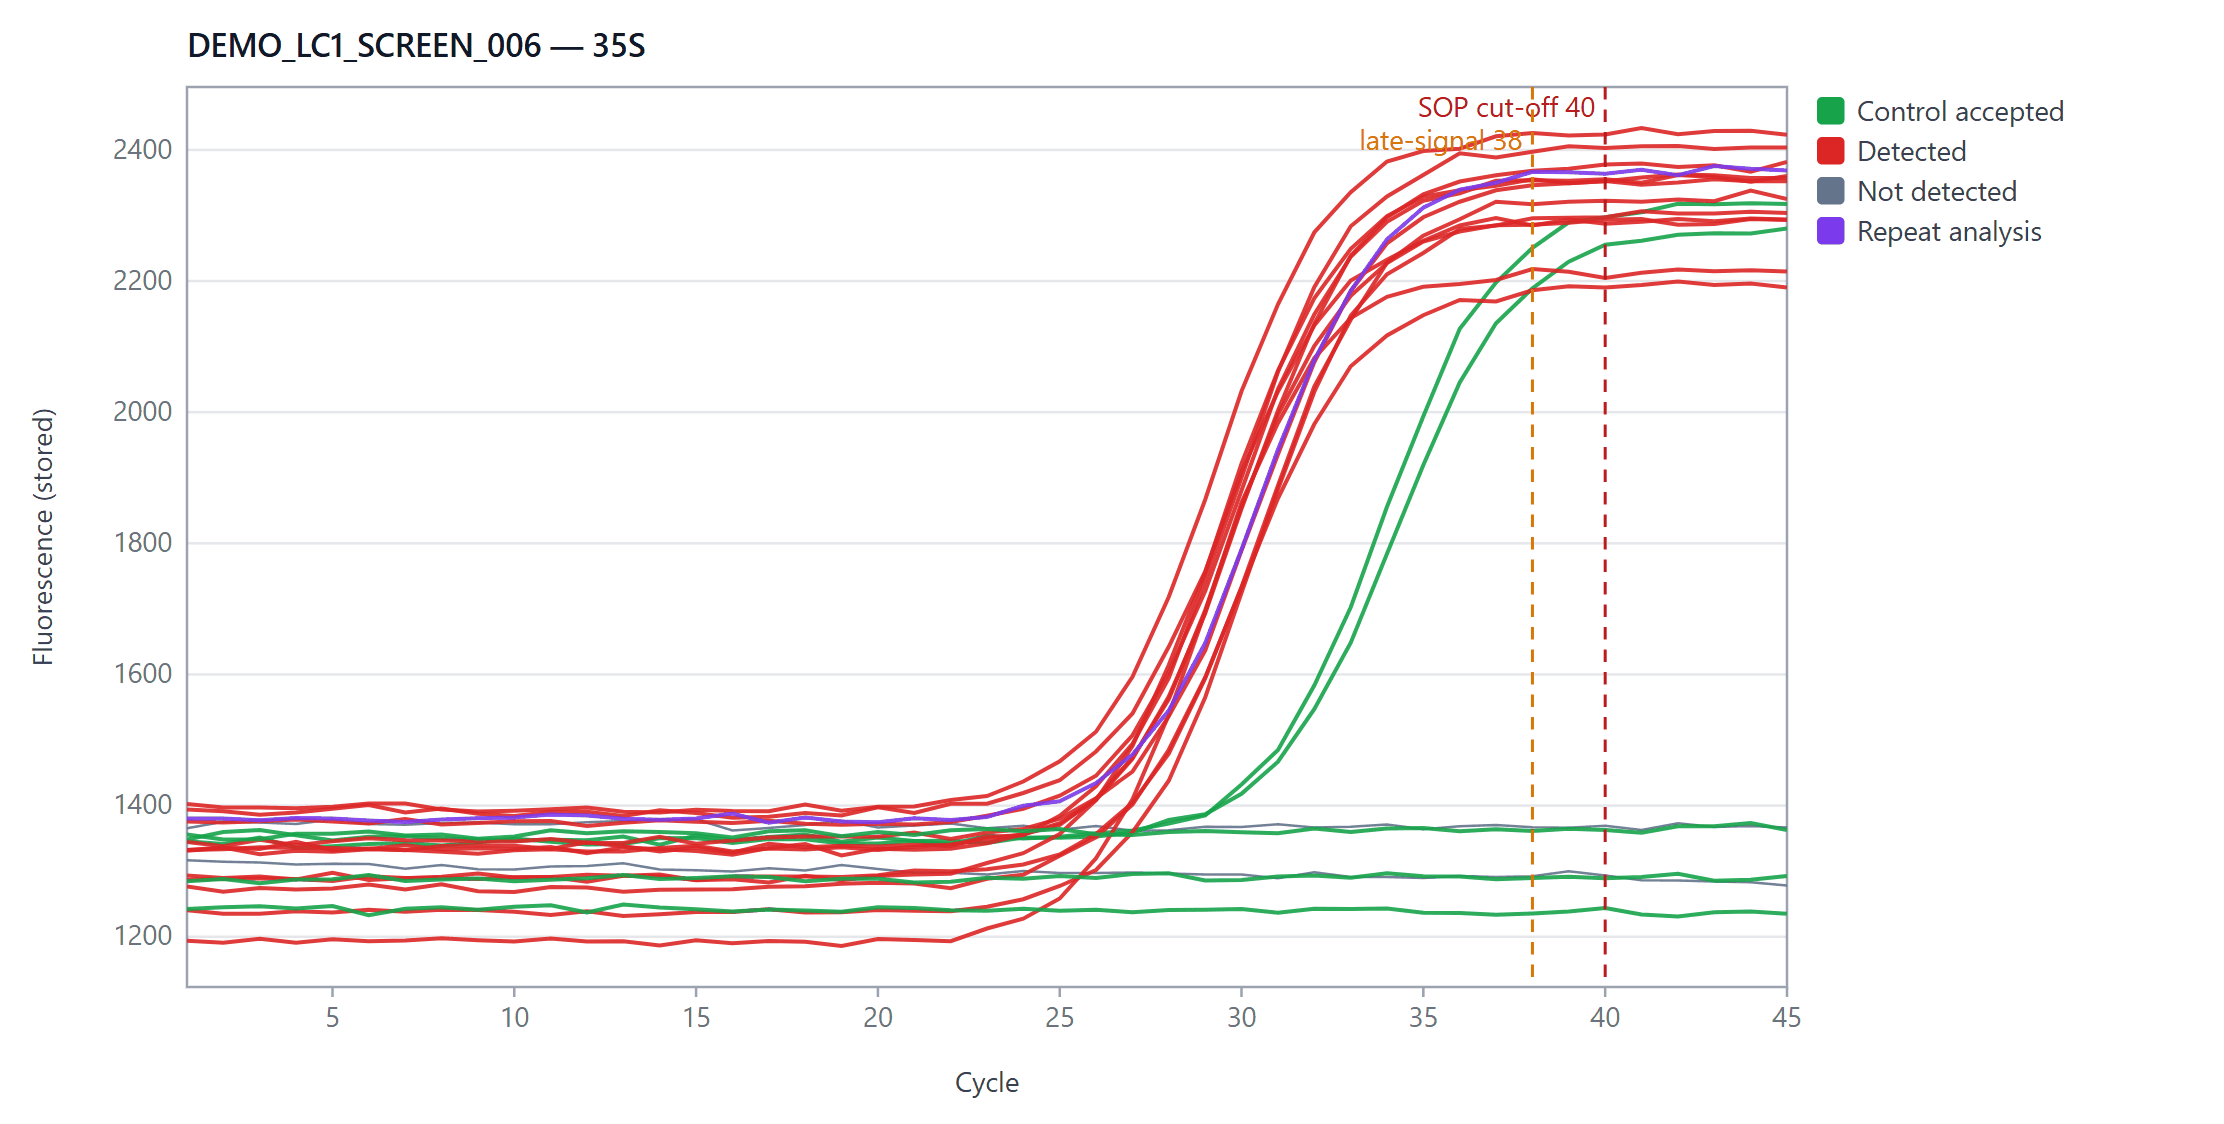
\includegraphics[width=\linewidth]{fig/g_LC_curves.png}\caption{.ixo instrument, 35S, accepted run}\label{fig:g_LC_curves}\end{subfigure}\hfill
\begin{subfigure}{0.49\linewidth}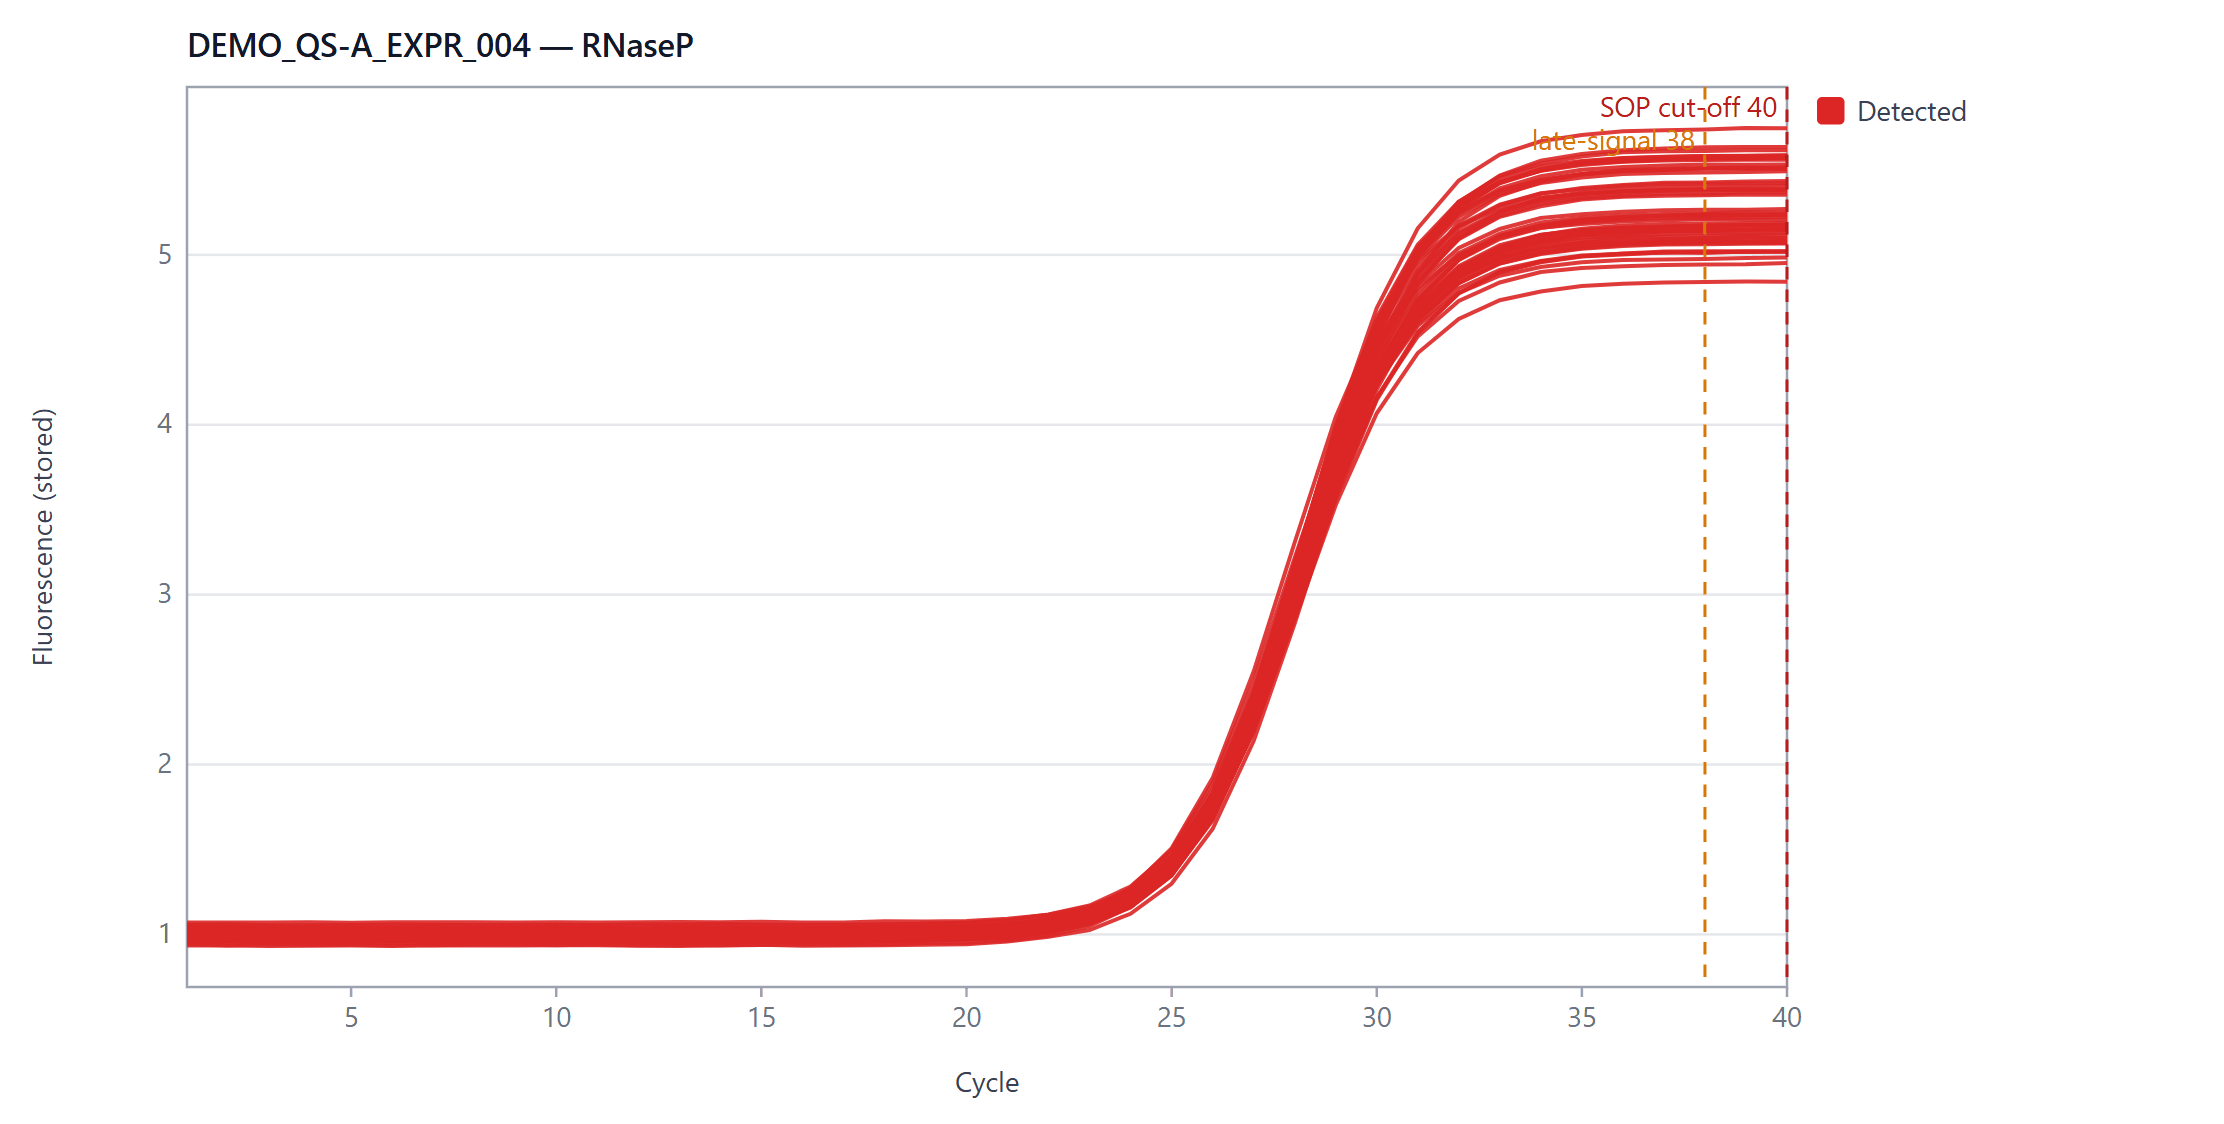
\includegraphics[width=\linewidth]{fig/g_QS_curves.png}\caption{.eds instrument, RAS}\label{fig:g_QS_curves}\end{subfigure}
\caption{\synthtag \texttt{curves} — amplification curves coloured by SOP outcome, with the SOP Cq cut-off and late-signal limit.}\label{fig:curves}
\end{figure}
\begin{figure}[htbp]\centering
\begin{subfigure}{0.49\linewidth}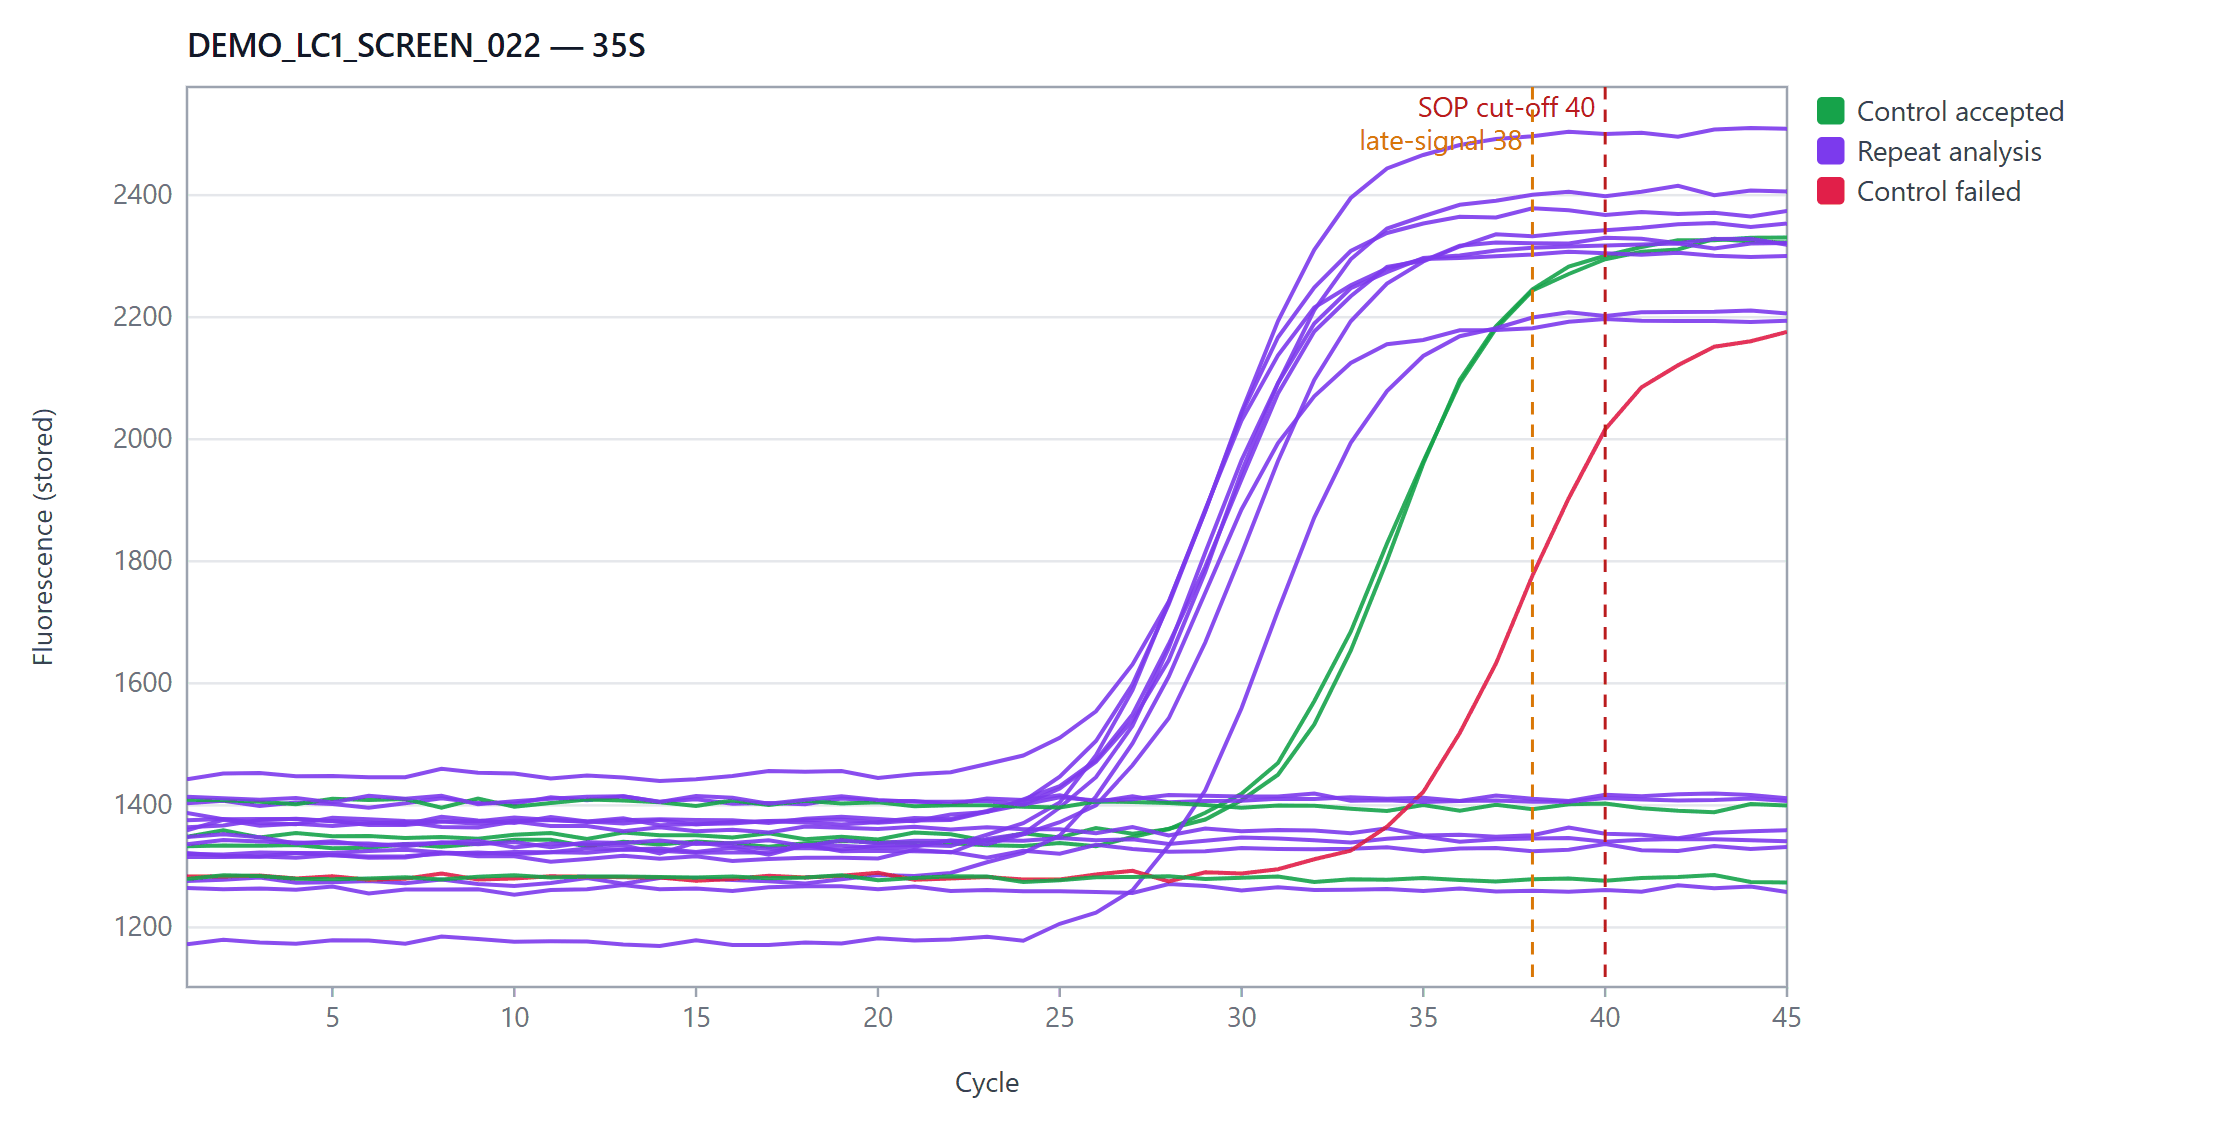
\includegraphics[width=\linewidth]{fig/g_LCX_curves.png}\caption{run 022: blank amplifies, run rejected}\label{fig:g_LCX_curves}\end{subfigure}\hfill
\begin{subfigure}{0.49\linewidth}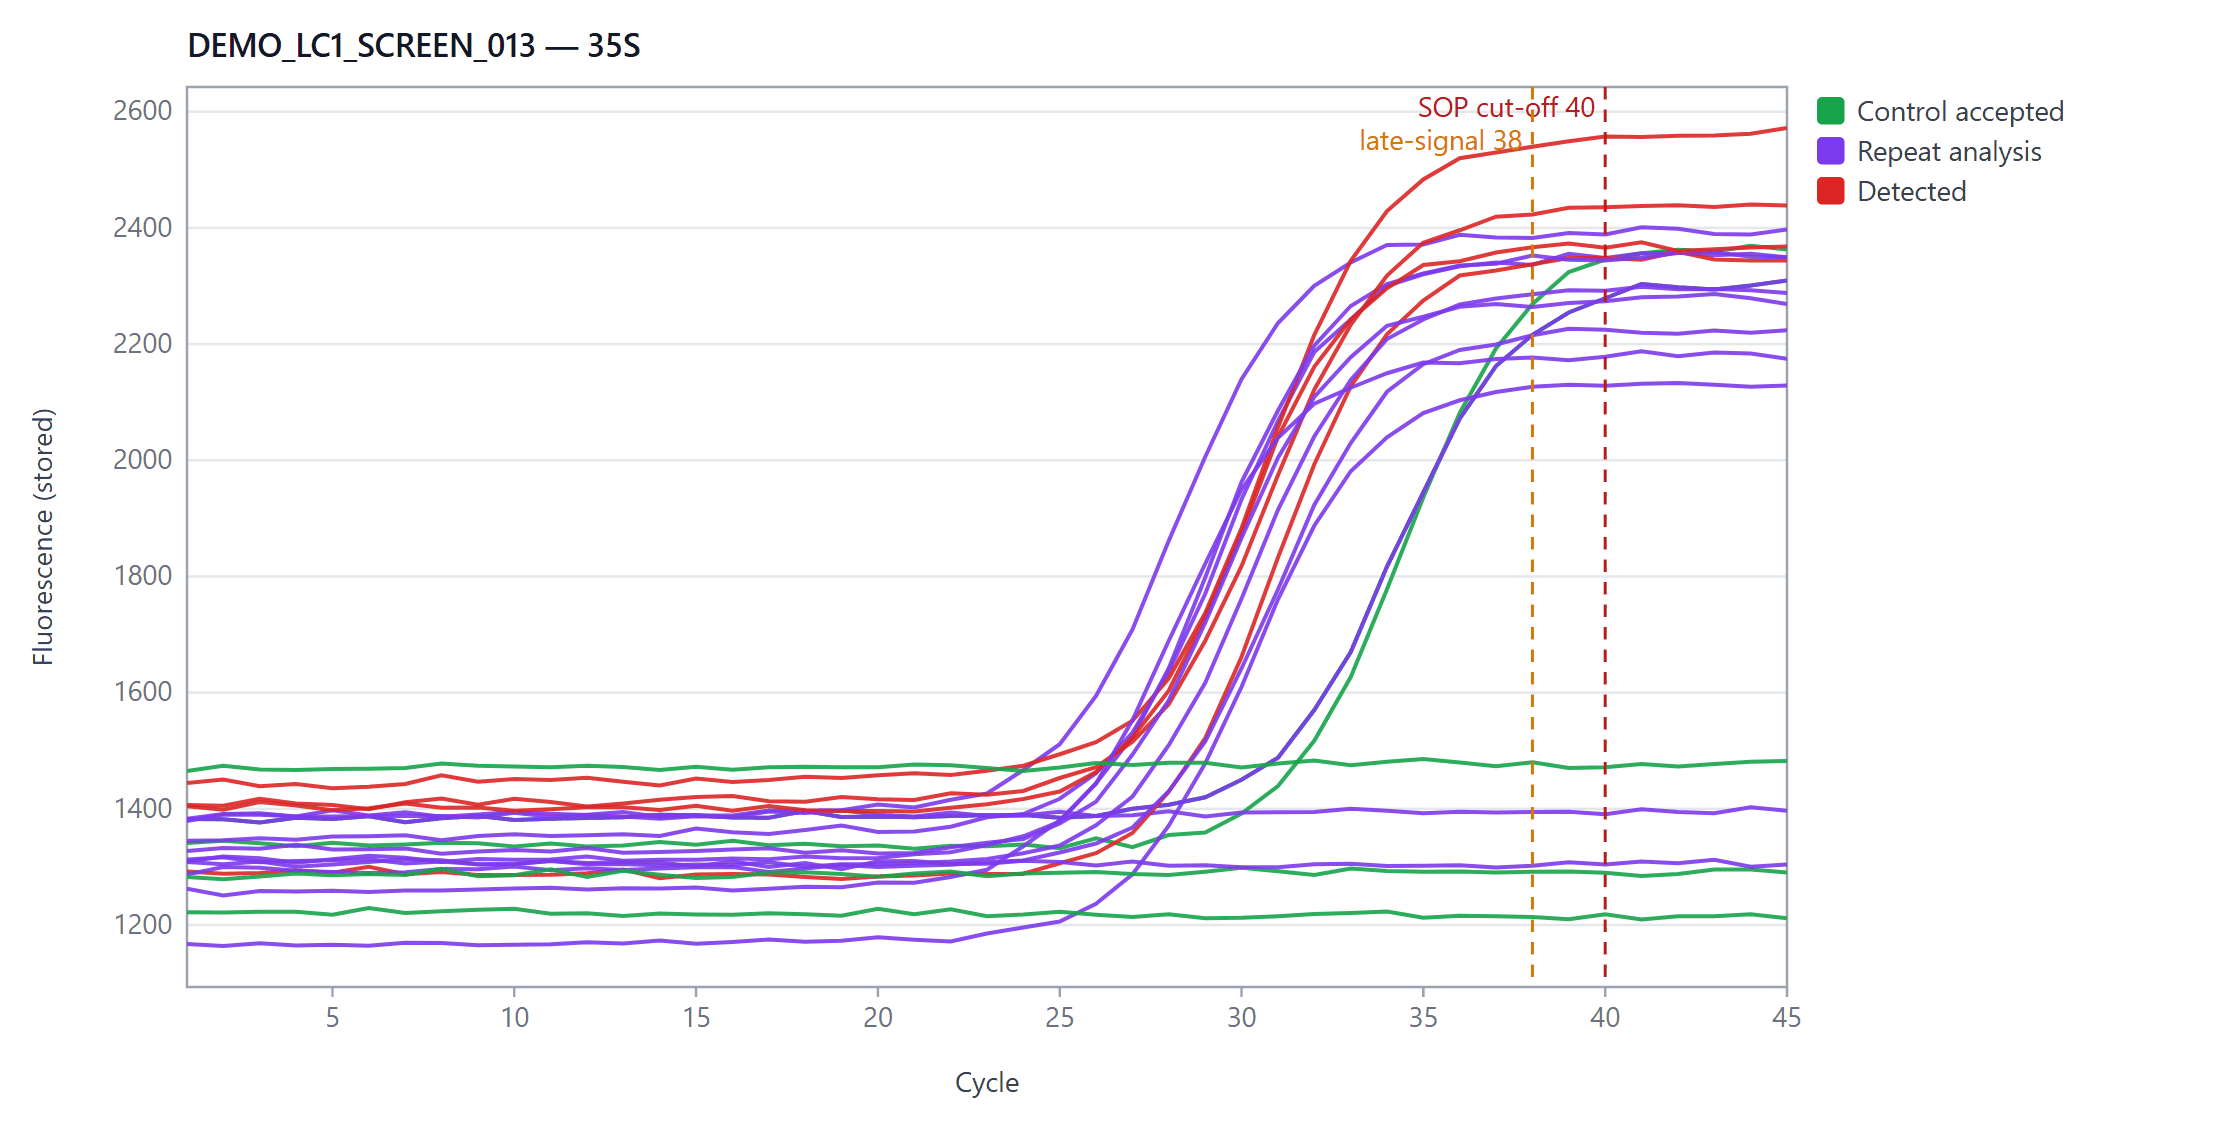
\includegraphics[width=\linewidth]{fig/g_LCC_curves.png}\caption{run 013: A03 is a copy of A01}\label{fig:g_LCC_curves}\end{subfigure}
\caption{\synthtag The planted events as the curves show them. In (a) the contaminated extraction blank (red, Cq 35.6) turns every result of the run into \emph{Invalid run}; in (b) two curves are identical point for point.}\label{fig:planted_curves}
\end{figure}
\fig[0.85]{g_QC_curves.png}{\texttt{curves} for a 10-point dilution series (\texttt{DEMO\_QS-C\_STDCURVE\_002}).}{g_QC_curves}
\fig[0.85]{g_LC_unanalysed.png}{\texttt{unanalysed} — curves of wells that are in no analysis. A signal here is a result nobody looked at.}{g_LC_unanalysed}
\begin{figure}[htbp]\centering
\begin{subfigure}{0.49\linewidth}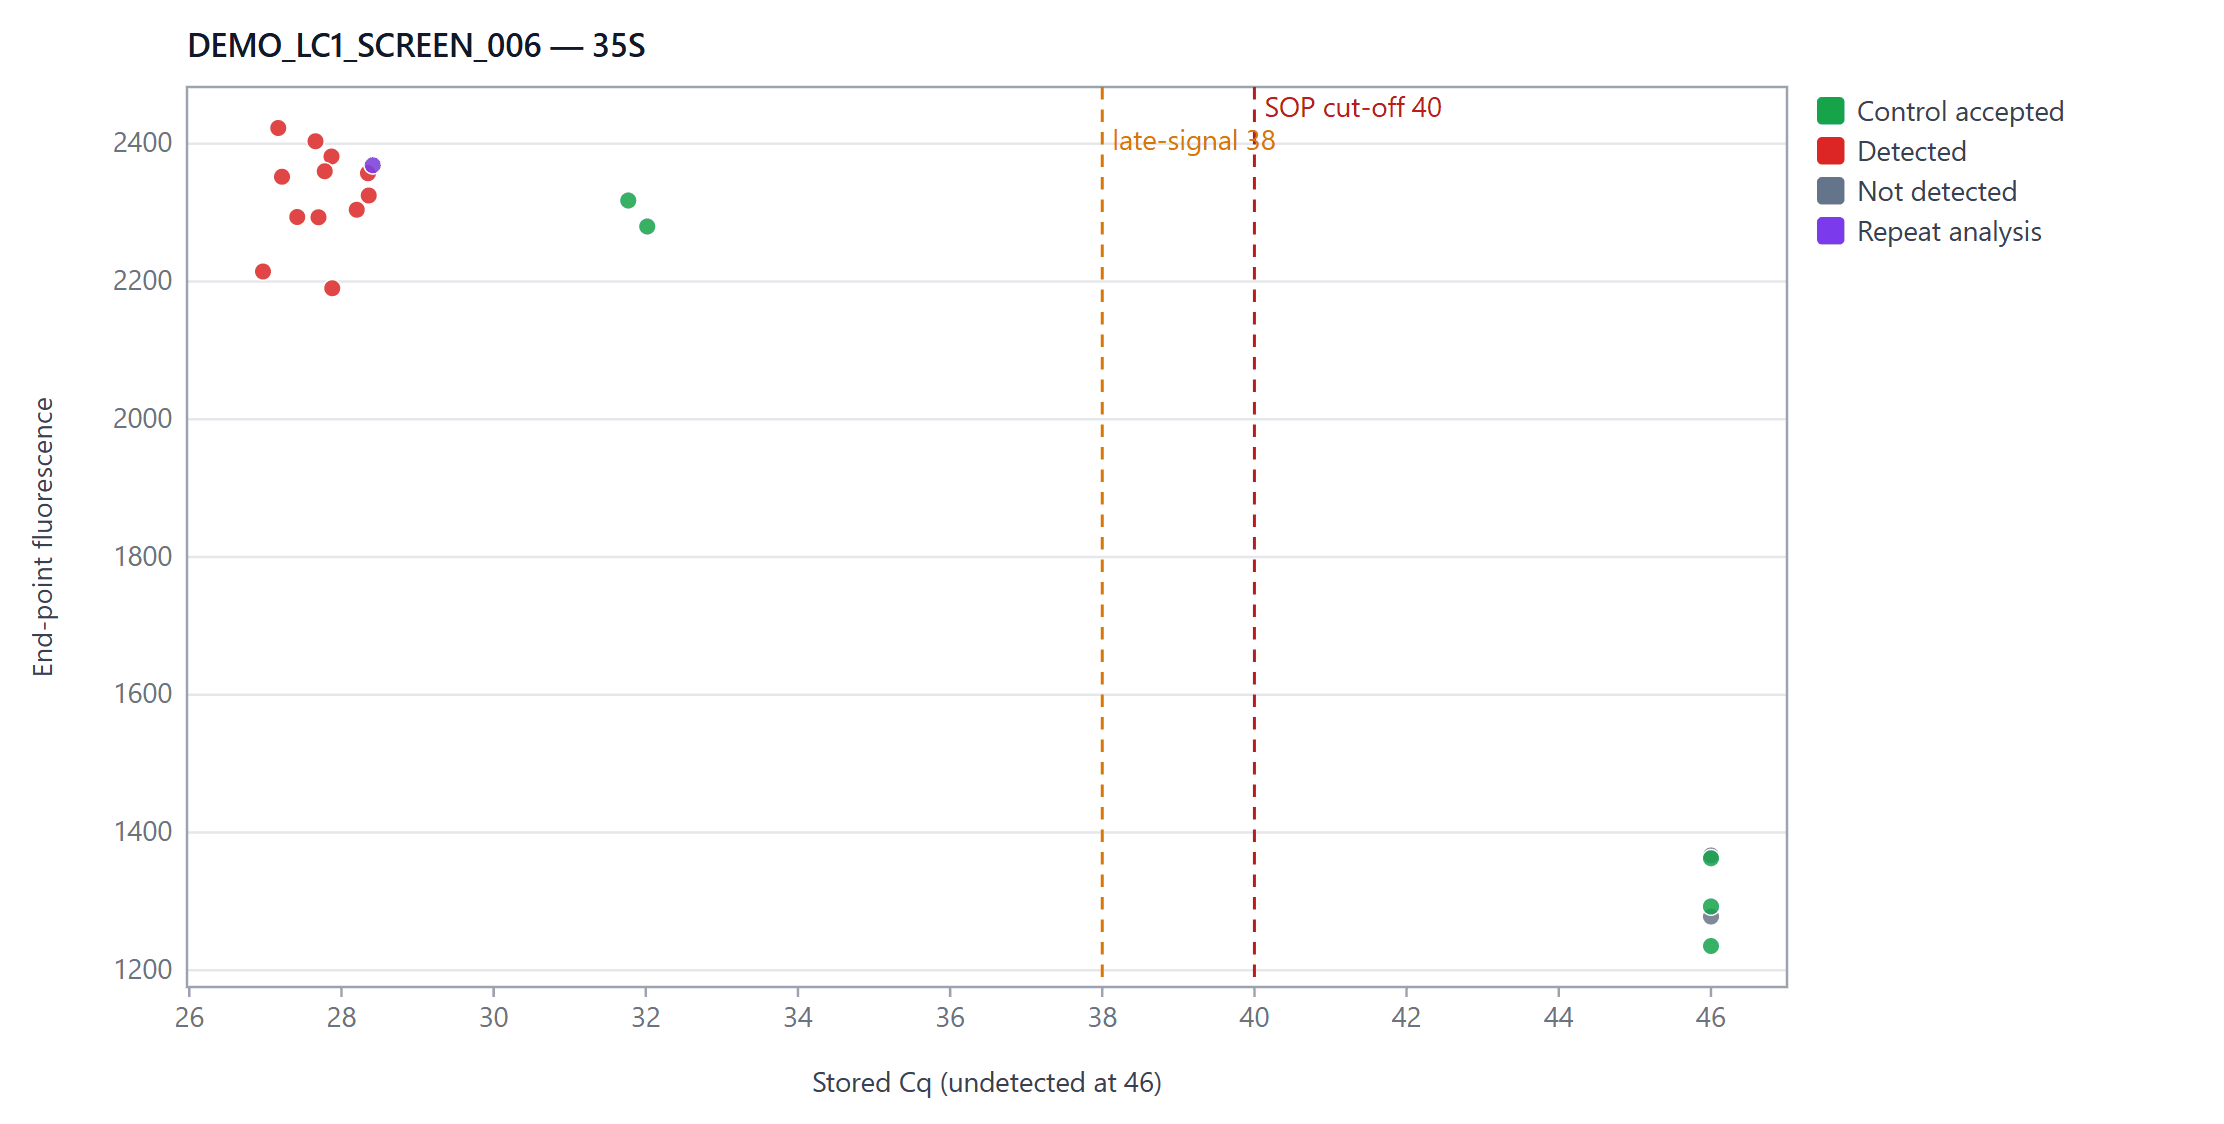
\includegraphics[width=\linewidth]{fig/g_LC_endpoint.png}\caption{\texttt{endpoint}: fluorescence against Cq}\end{subfigure}\hfill
\begin{subfigure}{0.49\linewidth}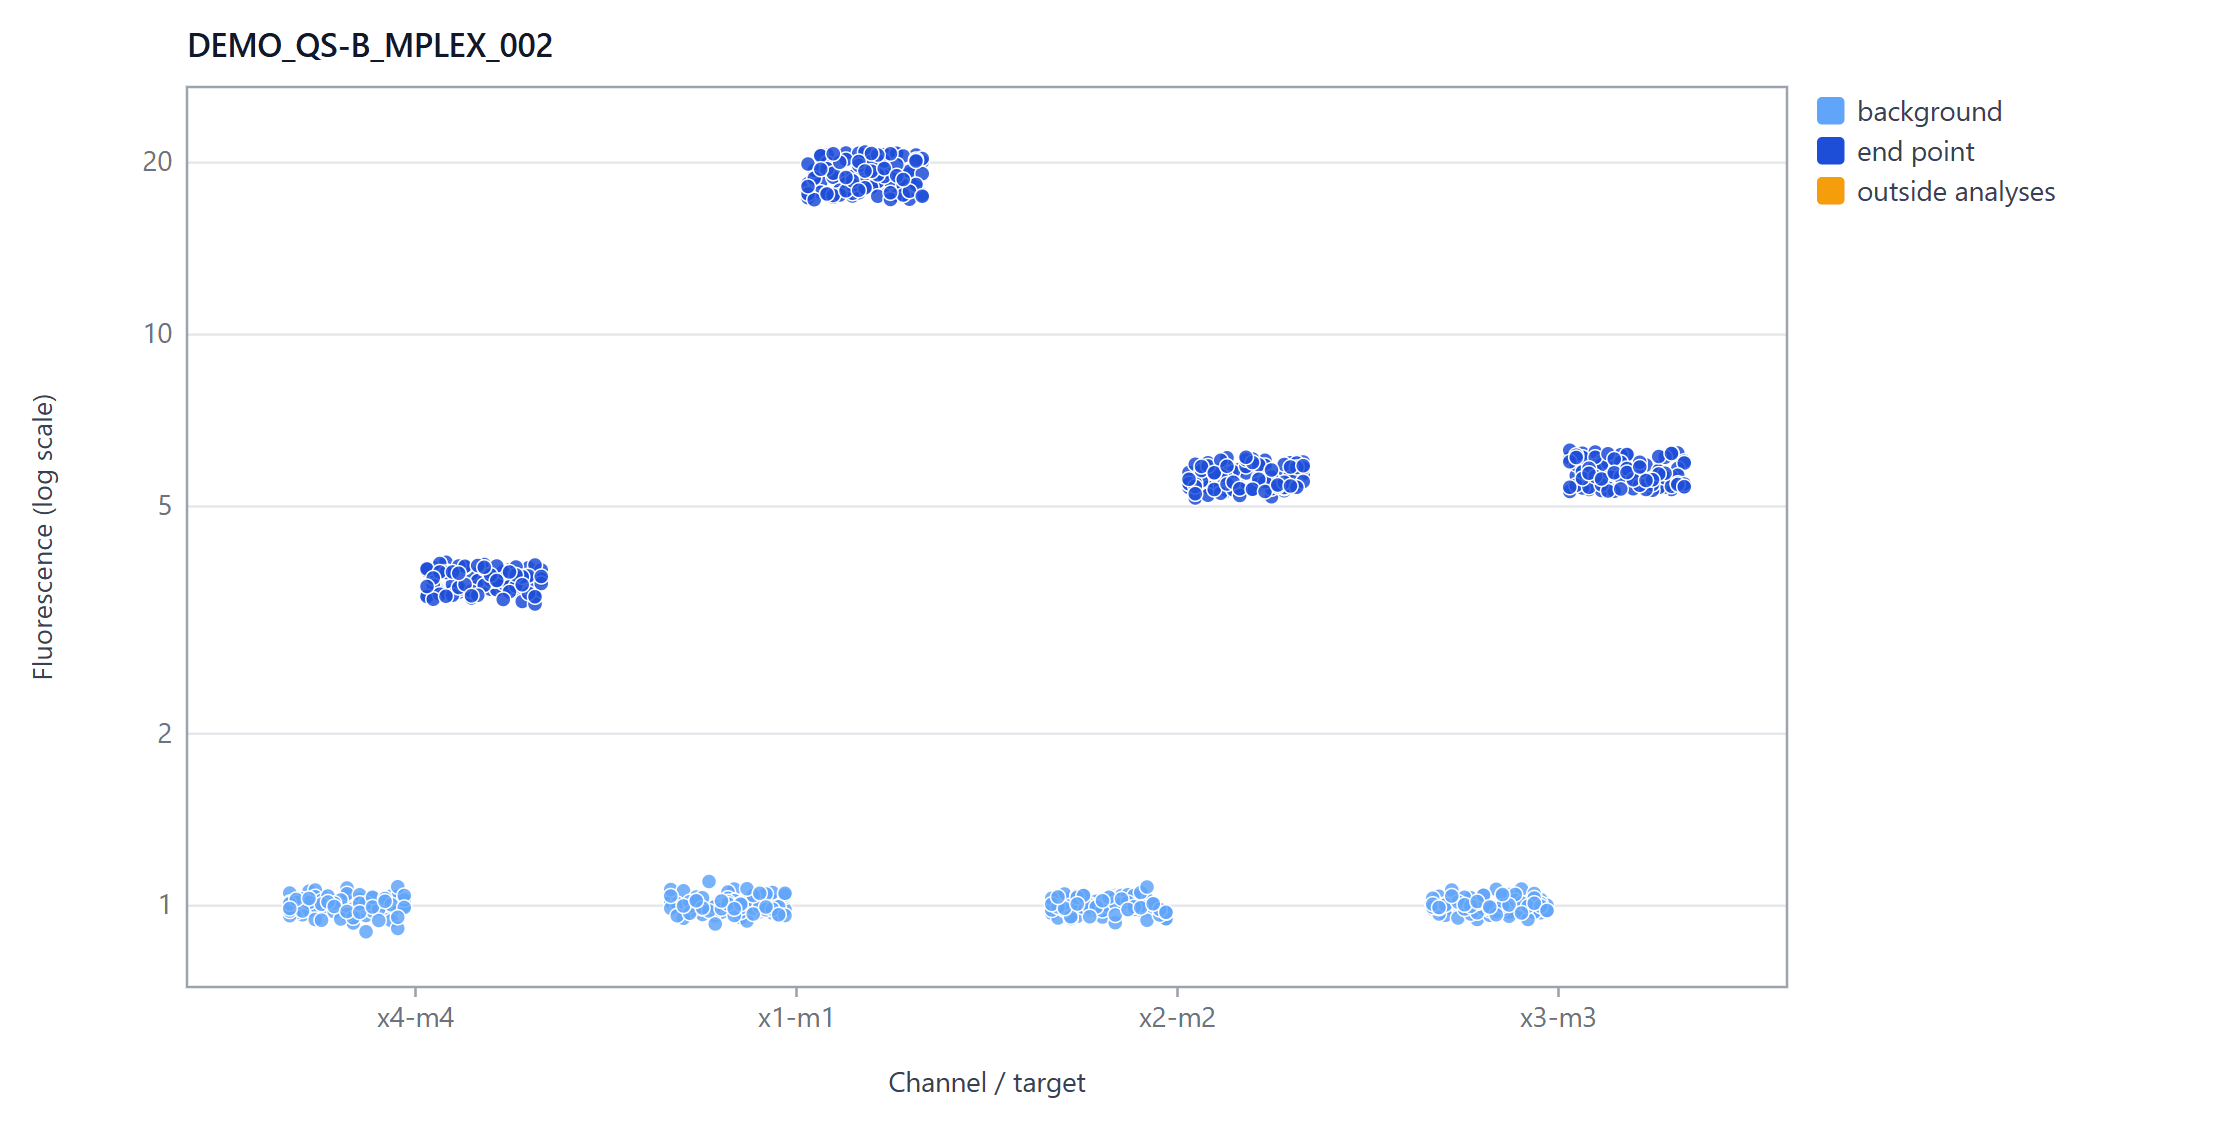
\includegraphics[width=\linewidth]{fig/g_QB_levels.png}\caption{\texttt{levels}: background and plateau per channel}\end{subfigure}
\caption{\synthtag Signal level graphs.}\label{fig:levels}
\end{figure}

\subsection*{Plate and results}
\begin{figure}[htbp]\centering
\begin{subfigure}{0.49\linewidth}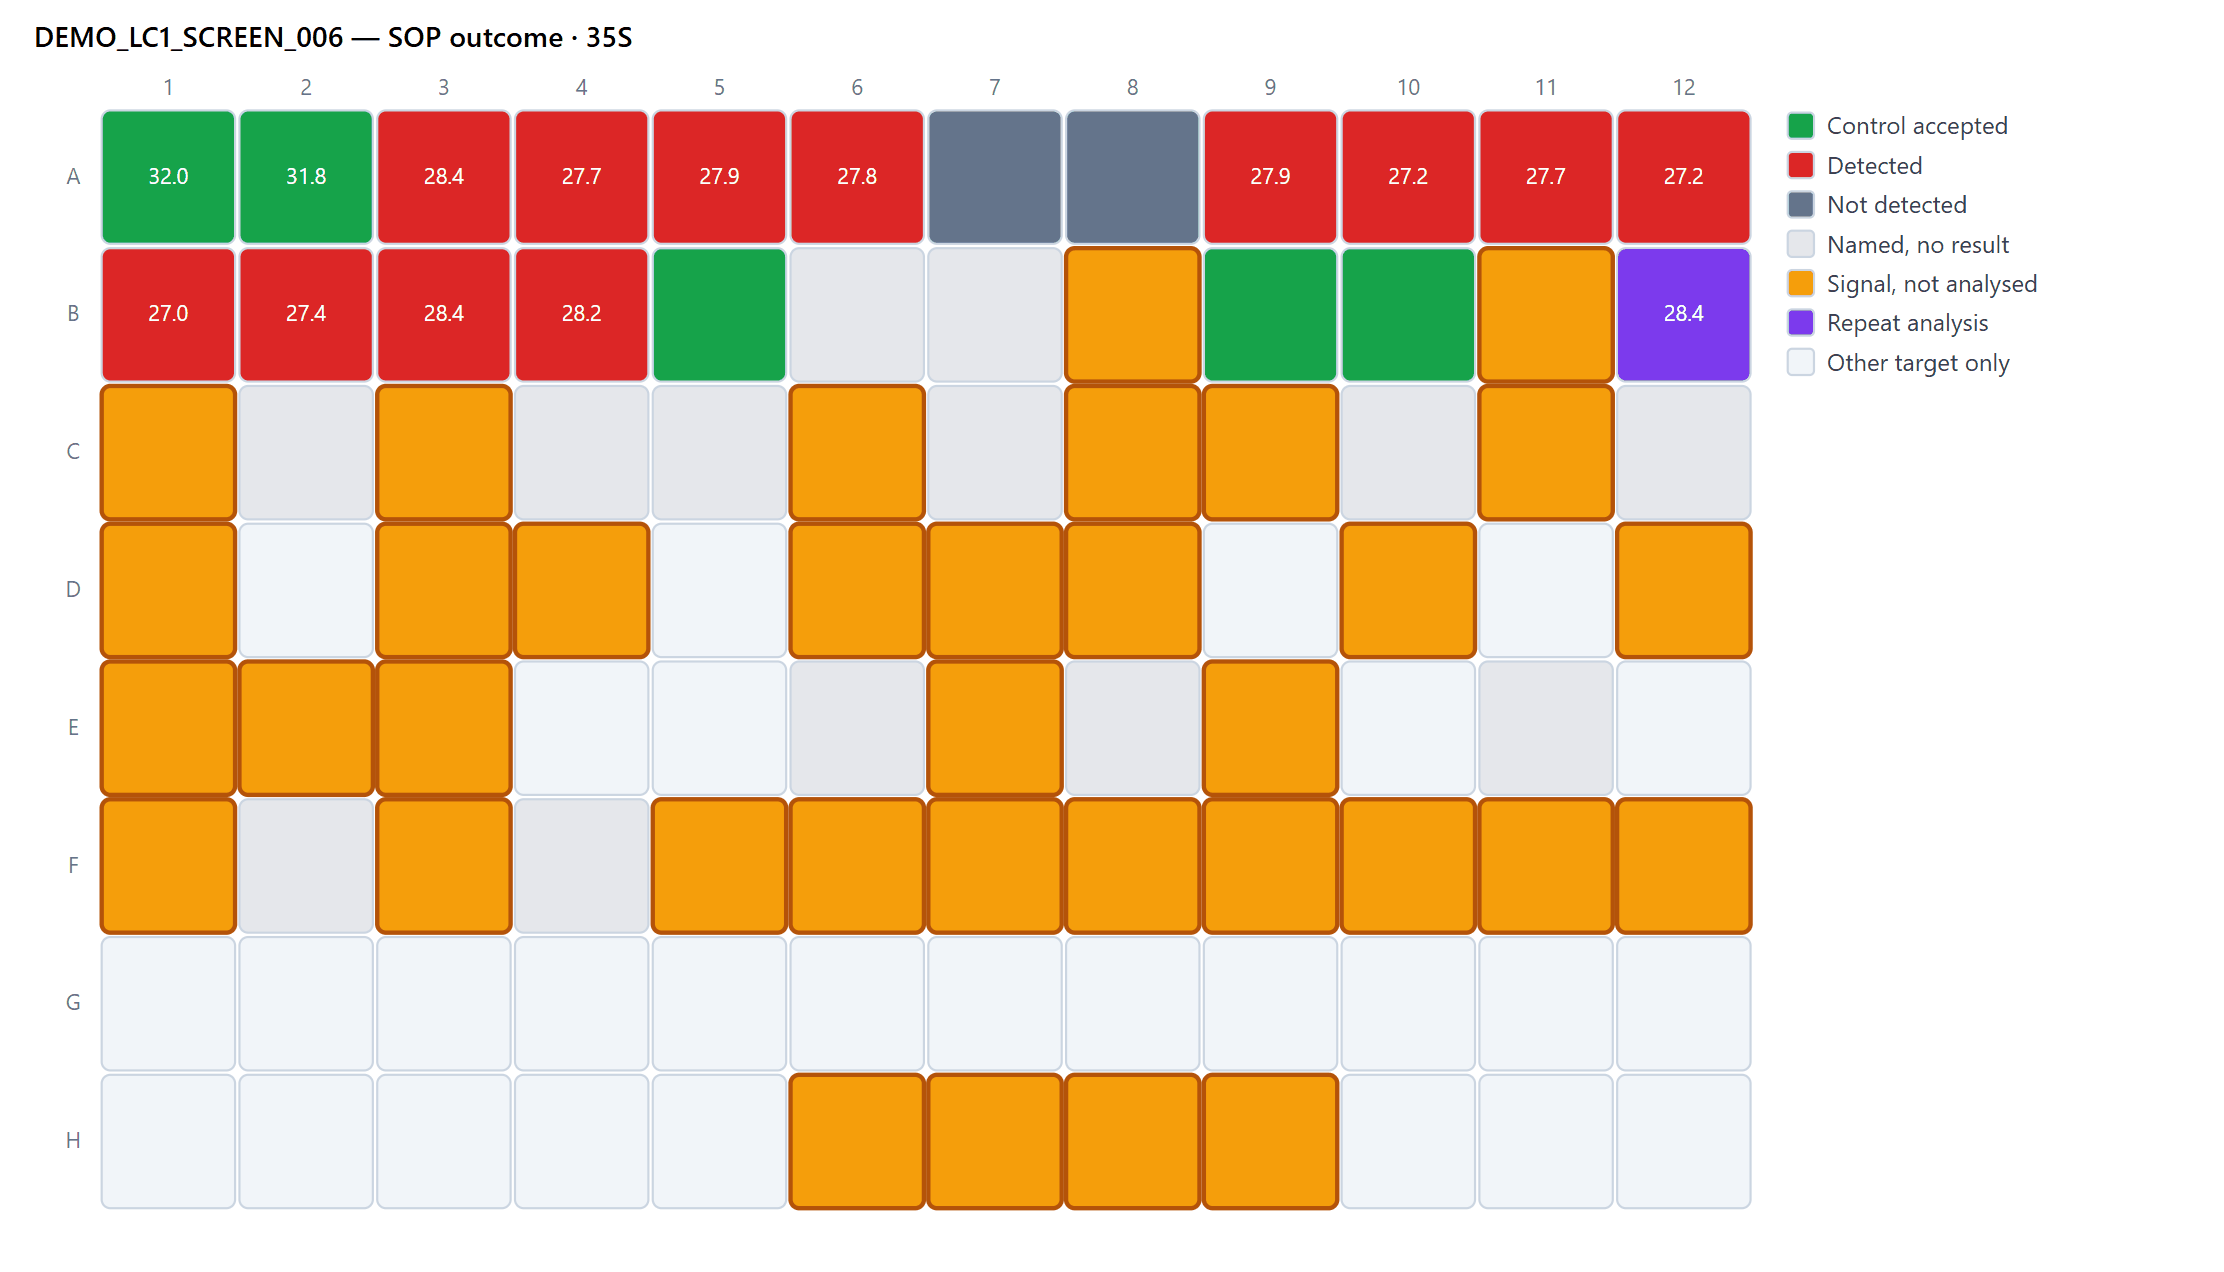
\includegraphics[width=\linewidth]{fig/g_LC_plate.png}\caption{.ixo instrument, 35S}\end{subfigure}\hfill
\begin{subfigure}{0.49\linewidth}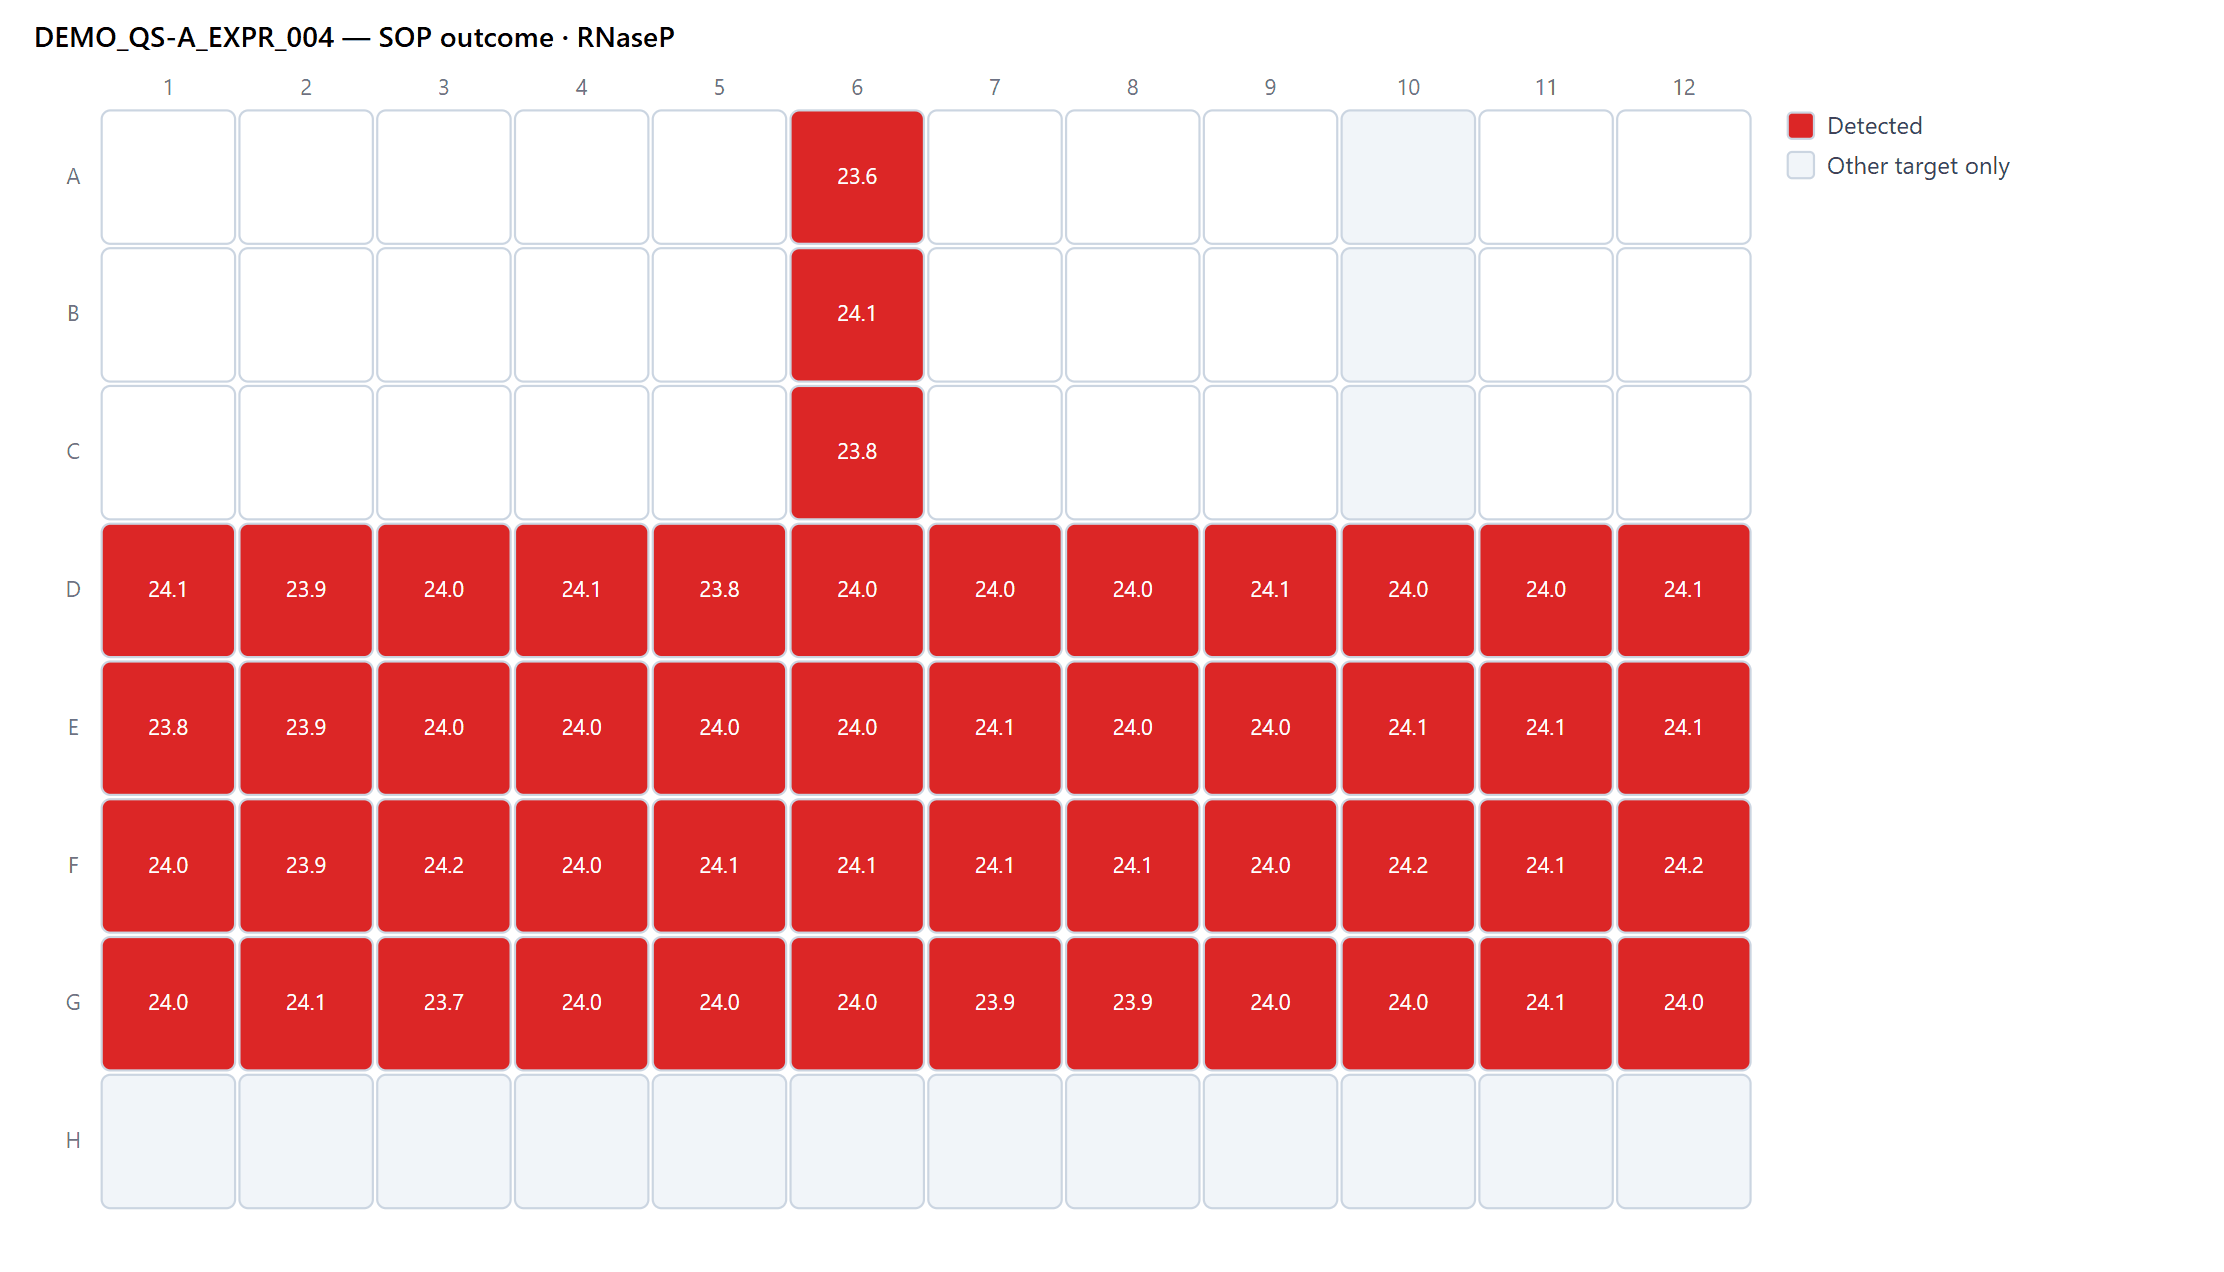
\includegraphics[width=\linewidth]{fig/g_QS_plate.png}\caption{.eds instrument, RAS}\end{subfigure}
\caption{\synthtag \texttt{plate} — heat map of the SOP outcome per well, with the stored Cq. Wells with a signal that is not analysed are outlined.}\label{fig:plate}
\end{figure}
\begin{figure}[htbp]\centering
\begin{subfigure}{0.49\linewidth}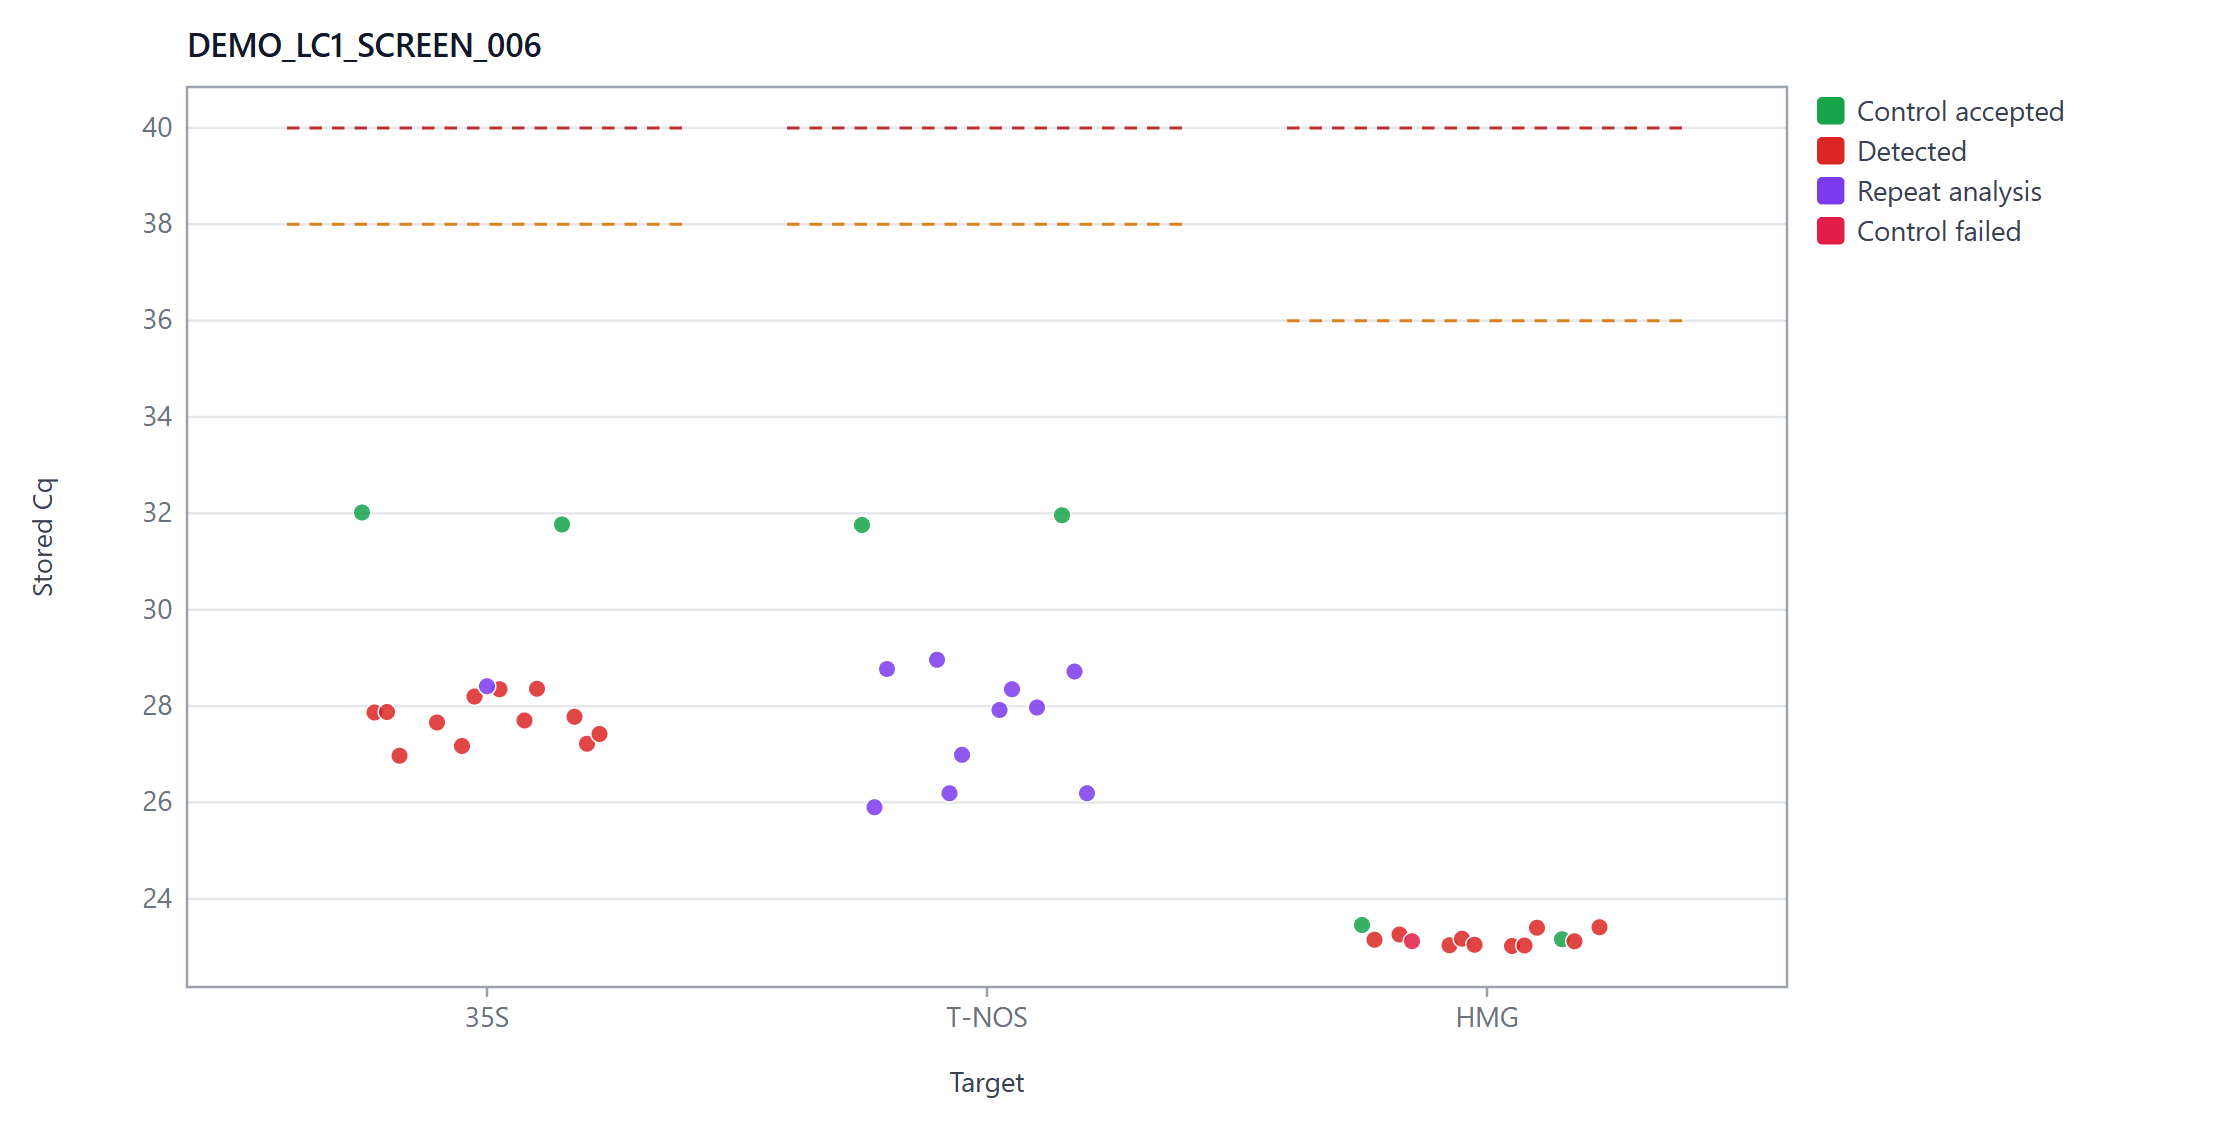
\includegraphics[width=\linewidth]{fig/g_LC_cqstrip.png}\caption{\texttt{cqstrip}}\end{subfigure}\hfill
\begin{subfigure}{0.49\linewidth}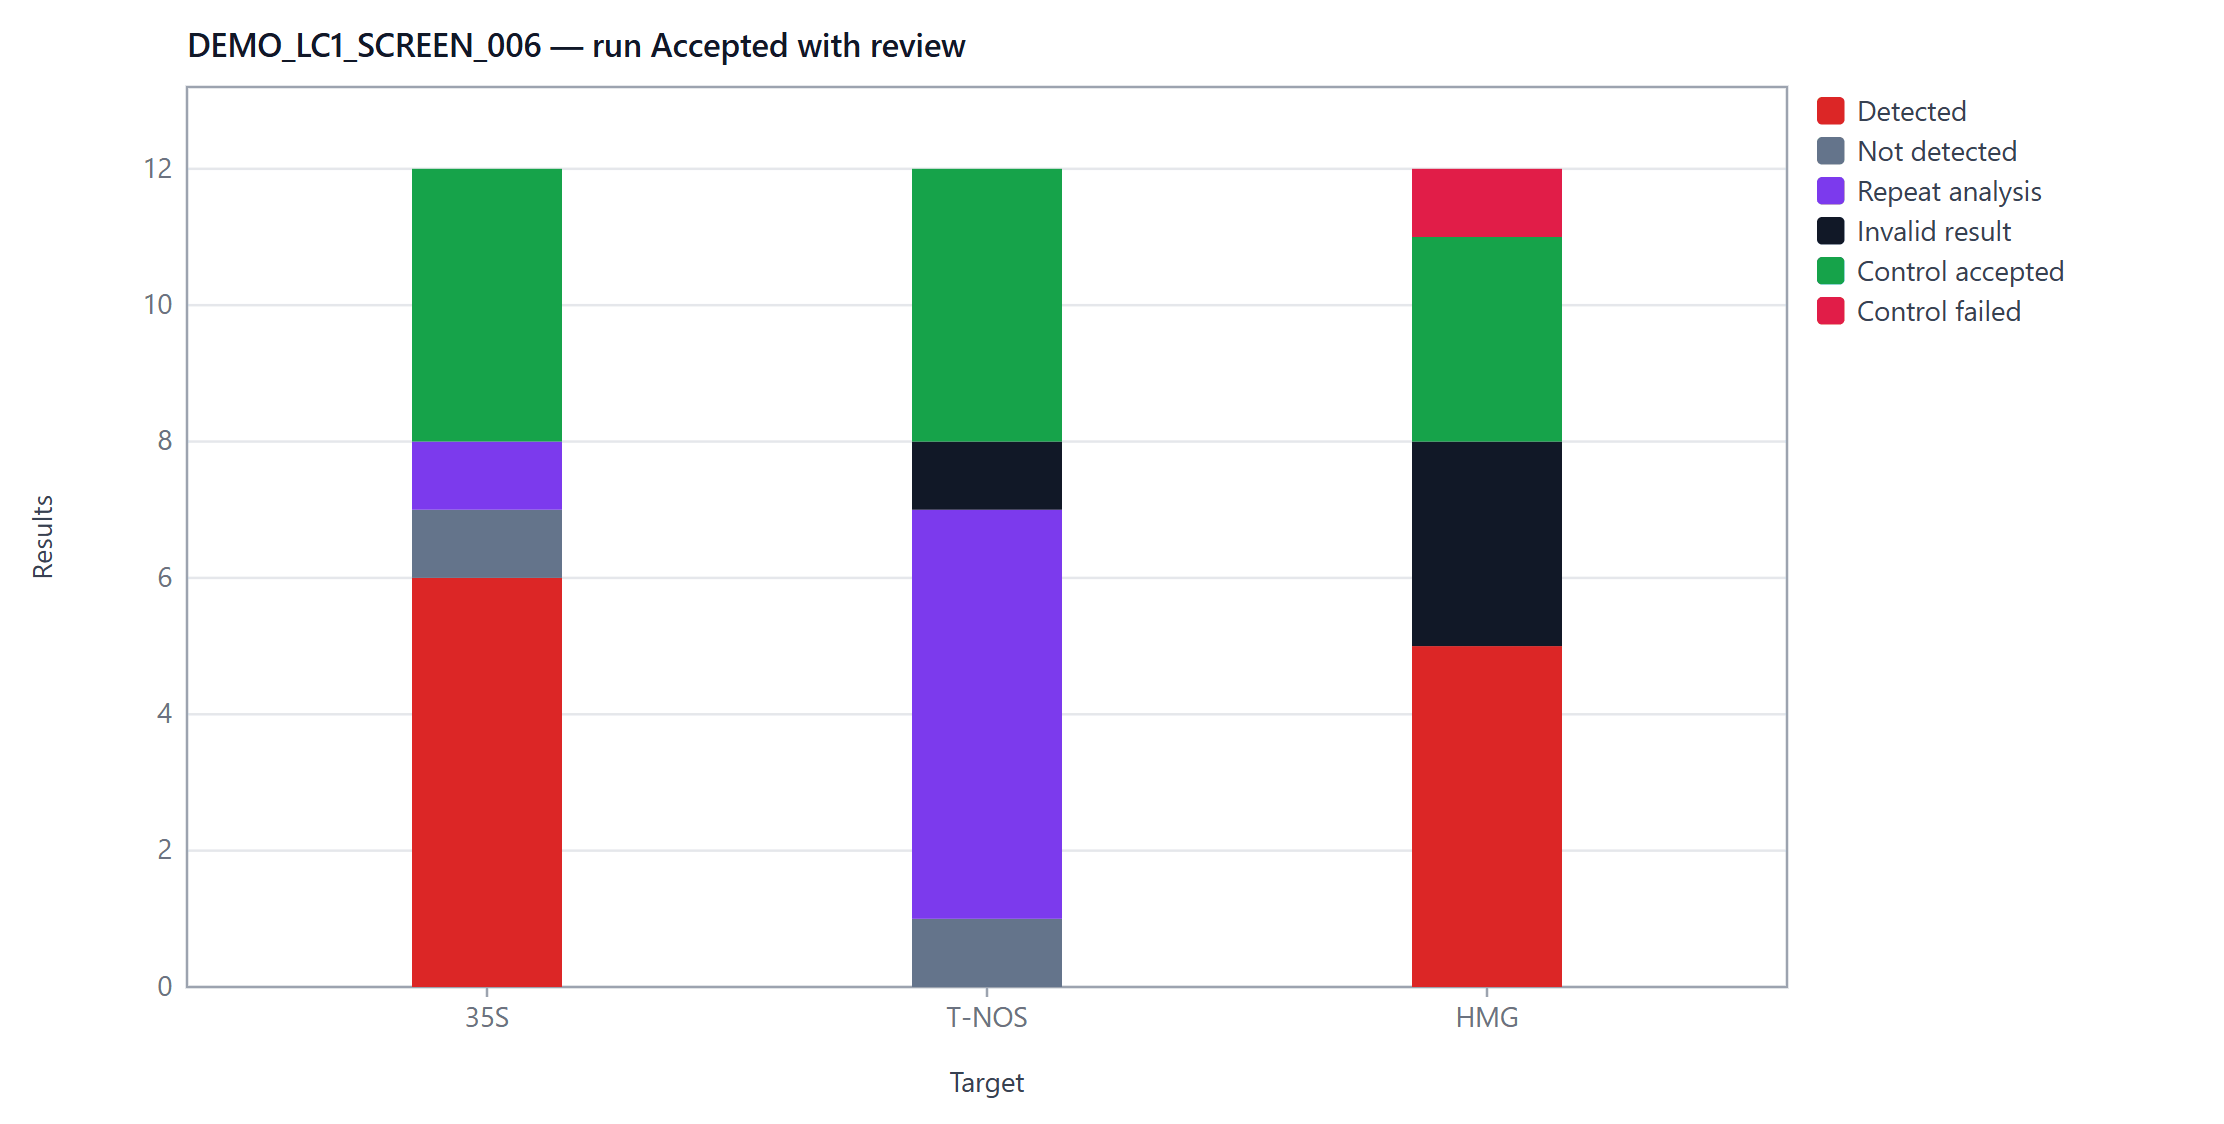
\includegraphics[width=\linewidth]{fig/g_LC_outcomes.png}\caption{\texttt{outcomes}}\end{subfigure}
\caption{\synthtag Cq by target with the SOP cut-offs, and SOP outcomes per target (\texttt{DEMO\_LC1\_SCREEN\_006}).}\label{fig:cqstrip}
\end{figure}
\begin{figure}[htbp]\centering
\begin{subfigure}{0.49\linewidth}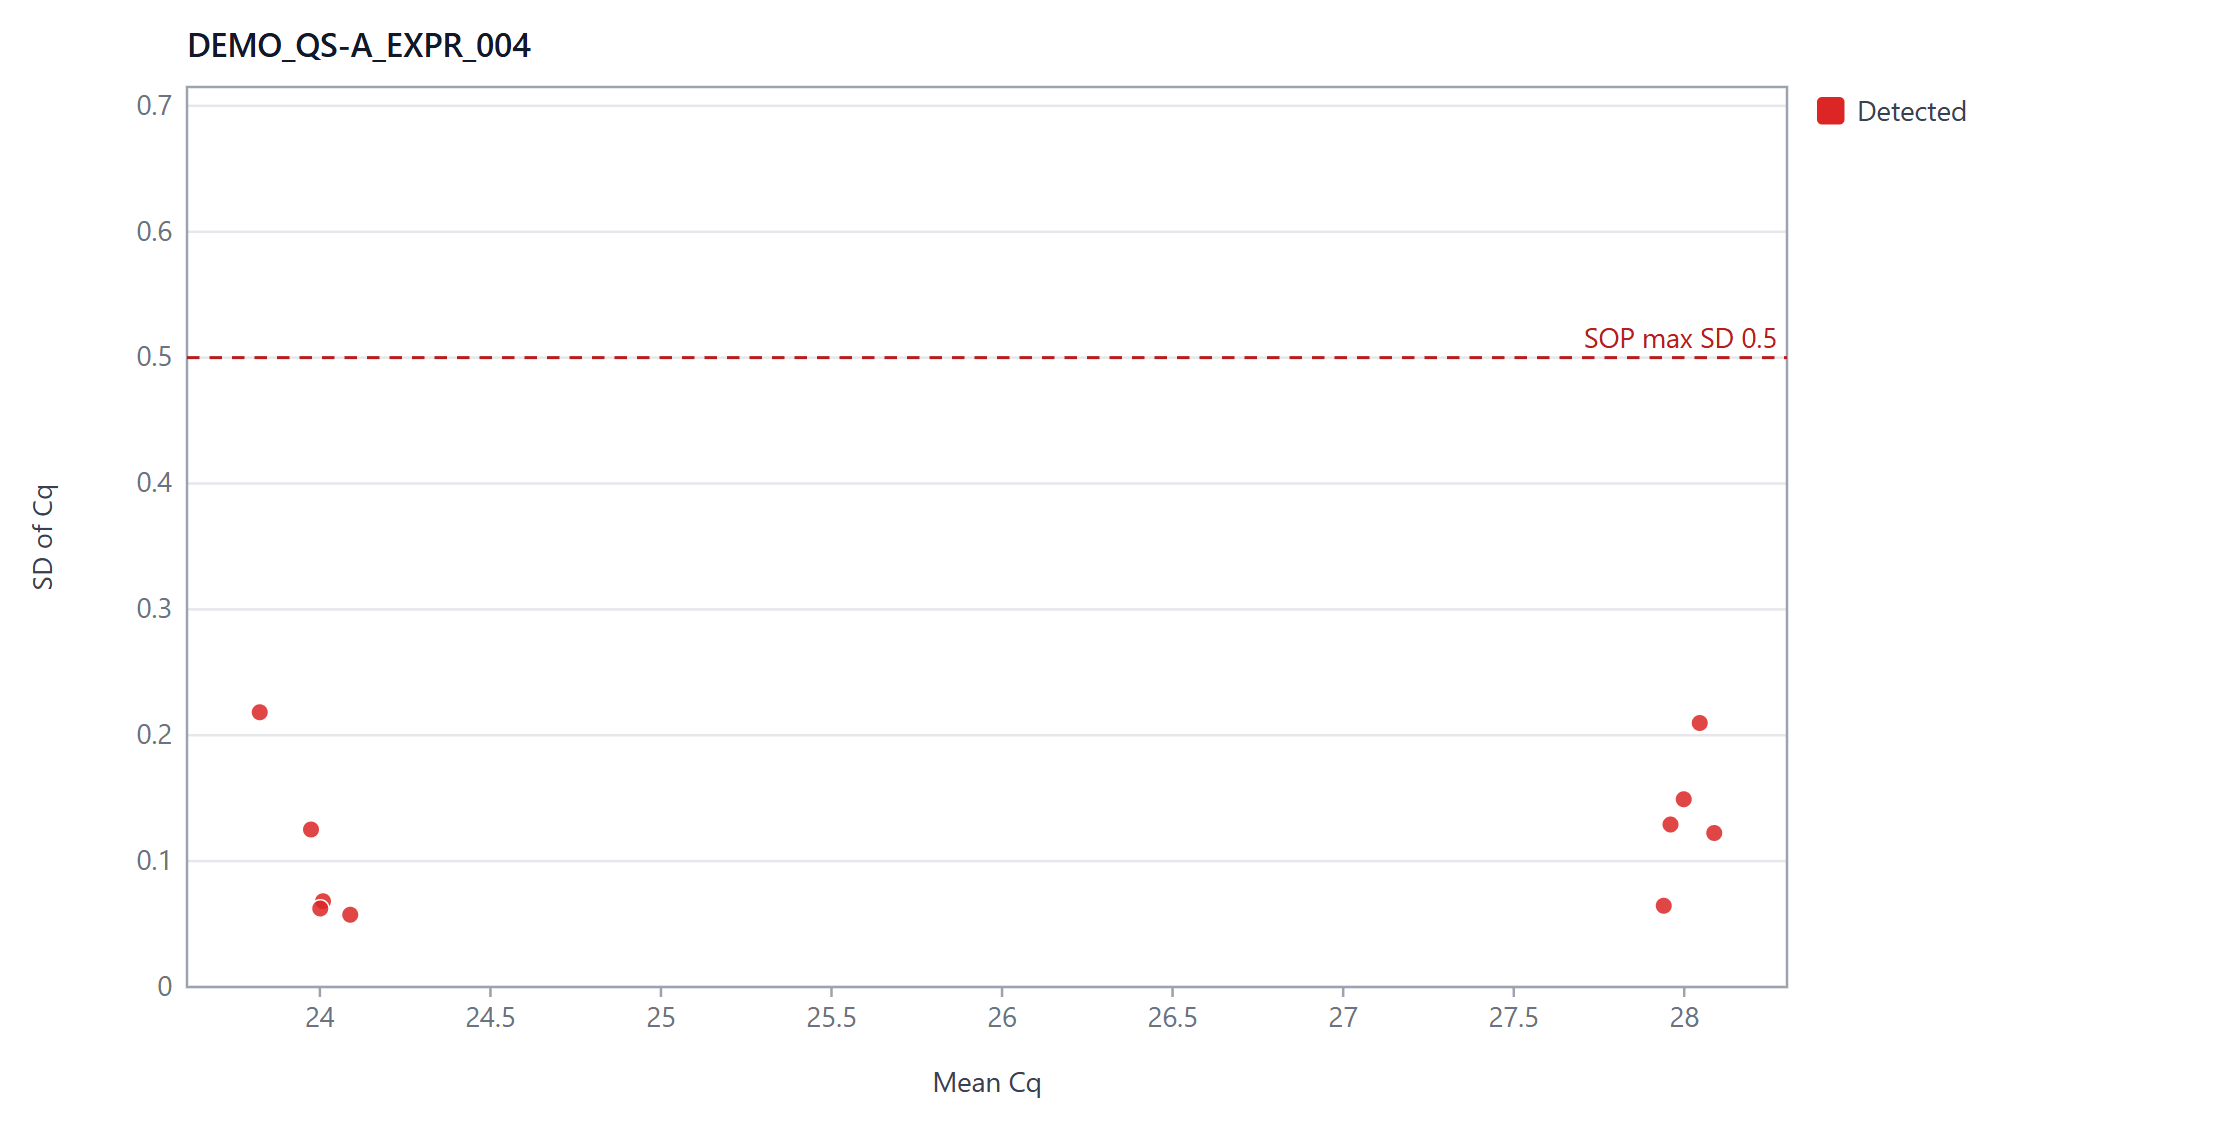
\includegraphics[width=\linewidth]{fig/g_QS_repsd.png}\caption{\texttt{repsd}: replicate SD against mean Cq}\end{subfigure}\hfill
\begin{subfigure}{0.49\linewidth}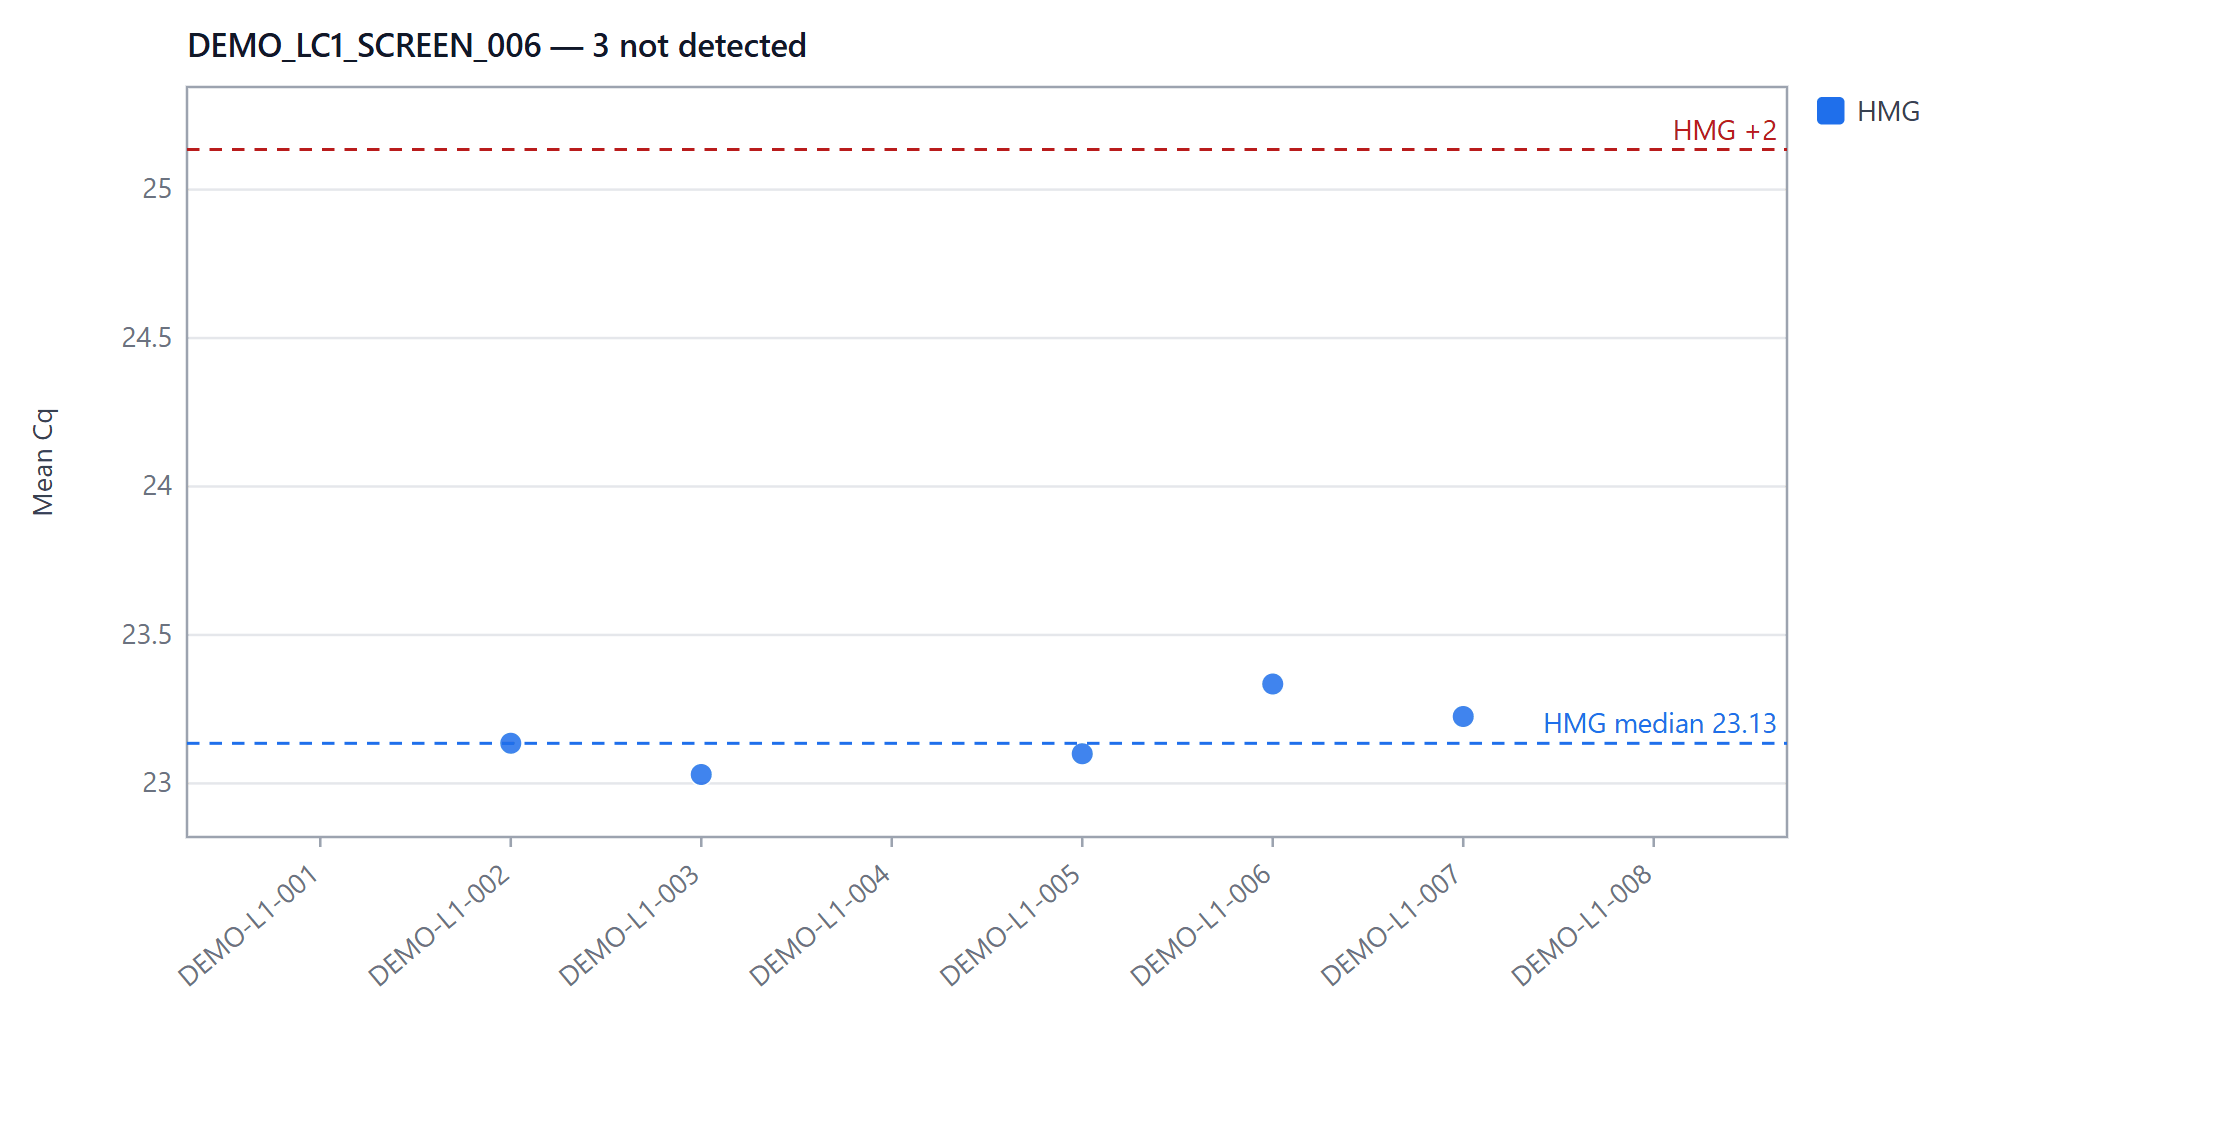
\includegraphics[width=\linewidth]{fig/g_LC_ic.png}\caption{\texttt{ic}: reference / IC Cq per sample}\end{subfigure}
\caption{\synthtag Replicate precision and reference-gene / internal-control graphs.}\label{fig:repsd_graphs}
\end{figure}
\fig[0.85]{g_QC_stdcurve.png}{\texttt{stdcurve} — standard curve of the synthetic dilution series with slope, R$^2$ and efficiency judged against the SOP (90--110\,\%, R$^2\ge0.98$, $\ge3$ logs).}{g_QC_stdcurve}
\fig[0.85]{g_QS_recalc.png}{\texttt{recalc} — stored Ct minus the Ct re-derived on the page from the stored $\Delta$Rn and threshold (.eds instrument). Points outside $\pm0.2$ would be flagged.}{g_QS_recalc}

\section{Graphs across all runs}
Cross-run graphs place the runs in date order; with more than 40 runs the axis shows dates instead of run names.

\par\medskip\noindent{\small\textbf{Listing}~\texttt{gRunDate()}\hfill\textcolor{gray}{HTML lines 5052--5052}}\par\nopagebreak
\lstinputlisting[style=vstyle,language=JavaScript,firstnumber=5052]{code/gRunDate.js}


\par\medskip\noindent{\small\textbf{Listing}~\texttt{gByDate()}\hfill\textcolor{gray}{HTML lines 5053--5053}}\par\nopagebreak
\lstinputlisting[style=vstyle,language=JavaScript,firstnumber=5053]{code/gByDate.js}


\par\medskip\noindent{\small\textbf{Listing}~\texttt{gRunTicks()}\hfill\textcolor{gray}{HTML lines 5054--5059}}\par\nopagebreak
\lstinputlisting[style=vstyle,language=JavaScript,firstnumber=5054]{code/gRunTicks.js}



\fig[0.85]{g_all_x_timeline.png}{\texttt{x\_timeline} — runs on a calendar (upper part): run (green), experiment created (blue), last change (red, joined by a dashed line).}{g_all_x_timeline}
\fig[0.9]{g_all_x_delay.png}{\texttt{x\_delay} — hours from run end to the last recorded change, log scale, SOP limit 72\,h. The planted 410\,h change of run 018 is red.}{g_all_x_delay}
\fig[0.8]{g_all_x_accept.png}{\texttt{x\_accept} — run acceptance grid: runs (rows) against the SOP criteria (columns), upper part.}{g_all_x_accept}
\fig[0.9]{g_all_x_outcomes.png}{\texttt{x\_outcomes} — stacked SOP outcomes per run.}{g_all_x_outcomes}
\fig[0.9]{g_all_x_control.png}{\texttt{x\_control} — descriptive control Cq across runs with the configured SOP range; pooled mean/SD lines were removed.}{g_all_x_control}
\fig[0.9]{g_all_x_signal.png}{\texttt{x\_signal} — median background (dashed) and end-point fluorescence (solid) per channel and run.}{g_all_x_signal}



\chapter{Tab 6 · Quality \& forensic review}\label{ch:review}

\section{Purpose}
The review tab answers file-integrity, result-consistency and control-identity questions. Its export contains plate map,
sample comparison, statistics, control charts, runs and QC, amplification curves and instrument records.
\readingnote{Use the sheet that answers the current check; the export does not replace the source instrument file.}

\figui{ui_review.png}{Review overview for the synthetic data set: experiments, stored and linked results, structural errors (the two planted errors), review findings.}{ui_review}

\section{The forensic log}
Every check writes events with a severity (\emph{error}, \emph{review}, \emph{info}), an area, a finding and the evidence.
The log collects structural checks, SOP findings and interpretation evidence. Control-chart alarm points are shown in Tab~2
and remain in the chart CSV/SVG exports; they are not duplicated here.

\par\medskip\noindent{\small\textbf{Listing}~\texttt{reviewForensicEvents()}\hfill\textcolor{gray}{HTML lines 4064--4071}}\par\nopagebreak
\lstinputlisting[style=vstyle,language=JavaScript,firstnumber=4064]{code/reviewForensicEvents.js}


\par\medskip\noindent{\small\textbf{Listing}~\texttt{reviewForensicEventsCoreUncached()}\hfill\textcolor{gray}{HTML lines 9068--9126}}\par\nopagebreak
\lstinputlisting[style=vstyle,language=JavaScript,firstnumber=9068]{code/reviewForensicEventsCore.js}


\par\medskip\noindent{\small\textbf{Listing}~\texttt{integrityEvents()}\hfill\textcolor{gray}{HTML lines 3762--3777}}\par\nopagebreak
\lstinputlisting[style=vstyle,language=JavaScript,firstnumber=3762]{code/integrityEvents.js}



\subsection*{Additional forensic checks}
\texttt{extraForensicEvents()} looks for identical curves or Cq values where independent data are expected (\emph{Copied data}),
dates in the wrong order, changes long after the run, stored calls that disagree with the SOP and similar signs.

\par\medskip\noindent{\small\textbf{Listing}~\texttt{extraForensicEventsUncached()}\hfill\textcolor{gray}{HTML lines 4659--4701}}\par\nopagebreak
\lstinputlisting[style=vstyle,language=JavaScript,firstnumber=4659]{code/extraForensicEvents.js}


\par\medskip\noindent{\small\textbf{Listing}~\texttt{westgardReview()}\hfill\textcolor{gray}{HTML lines 9232--9249}}\par\nopagebreak
\lstinputlisting[style=vstyle,language=JavaScript,firstnumber=9232]{code/westgardReview.js}



Exact control names are now the default. The SC profile adds a canonical-family view for descriptive pooling while retaining
the original sample text. Review baselines use the initial configured run count; pooling does not change stored values.

\section{Findings on the synthetic data}
{\footnotesize
\begin{longtable}{@{}lll@{}}
\toprule \textbf{Column 1} & \textbf{Column 2} & \textbf{Column 3} \\\midrule\endfirsthead
\toprule \textbf{Column 1} & \textbf{Column 2} & \textbf{Column 3} \\\midrule\endhead
error & Copied data & 1 \\\hline
review & Analysis membership & 3684 \\\hline
review & Control chart B-H3c & 122 \\\hline
review & SOP: DEMO laboratory SOP (synthetic example) & 102 \\\hline
review & Control chart B-H1 & 40 \\\hline
review & Detection format & 38 \\\hline
review & Control chart A-H4 & 35 \\\hline
review & Control chart B-H15 & 32 \\\hline
review & Control chart B-H11 & 31 \\\hline
review & Control chart B-S9 & 31 \\\hline
review & Control chart B-O1 & 31 \\\hline
review & Control chart B-H3 & 30 \\\hline
review & Control chart B-H3b & 30 \\\hline
review & Control chart B-H4 & 30 \\\hline
review & Control chart A-M1 & 27 \\\hline
review & Control chart B-H2 & 22 \\\hline
review & Timeline & 20 \\\hline
review & Provenance & 19 \\\hline
review & Control chart A-S4 & 13 \\\hline
review & Control chart B-H10b & 11 \\\hline
review & Control chart B-H5 & 10 \\\hline
review & Control chart B-H10 & 10 \\\hline
\bottomrule
\end{longtable}}


{\footnotesize
\begin{longtable}{@{}llll@{}}
\toprule \textbf{Experiment} & \textbf{Severity} & \textbf{Area} & \textbf{Finding and evidence} \\\midrule\endfirsthead
\toprule \textbf{Experiment} & \textbf{Severity} & \textbf{Area} & \textbf{Finding and evidence} \\\midrule\endhead
\texttt{DEMO\_LC1\_SCREEN\_013} & error & Copied data & 1 well pair(s) carry identical… \\\hline
\texttt{DEMO\_LC1\_SCREEN\_018} & review & Timeline & Last recorded change 410.0 h a… \\\hline
\texttt{DEMO\_LC1\_SCREEN\_018} & review & SOP: DEMO laboratory SOP (synt… & Control result — Reference che… \\\hline
\texttt{DEMO\_LC1\_SCREEN\_018} & review & SOP: DEMO laboratory SOP (synt… & Edited within the allowed wind… \\\hline
\texttt{DEMO\_LC1\_SCREEN\_018} & review & SOP: DEMO laboratory SOP (synt… & 15 result(s) need action (Repe… \\\hline
\bottomrule
\end{longtable}}



The synthetic gallery includes a dilution-series example in which one NTC shows a late signal; the example demonstrates a
failed negative-control rule without reproducing a laboratory result.

Most review findings are expected for this data set: many wells are named but not included in an analysis
(\emph{Analysis membership}), and the history contains the planted trends, which the control charts report as alarms.
\readingnote{A red point is outside a displayed limit; an amber point is an enabled pattern rule inside the limits. Both
are review prompts. A missing chart series means that its data or eligibility requirements were not available.}

\fig[0.9]{g_all_x_findings.png}{\texttt{x\_findings} — Pareto of error and review findings by area.}{findings}



\chapter{Tab 7 · Open formats}\label{ch:values}

Tab 6 writes the stored values and other data in formats that other tools read. It does not recalculate the instrument's Cq,
Ct, calls or fluorescence. Each download names the tool that consumes it and what was checked.

\begin{center}\small
\begin{tabular}{@{}p{4.3cm}p{10.9cm}@{}}\toprule
Download & Content and consumer\\\midrule
Cq values (CSV) & every stored crossing point with well, sample, target, role and call — the plain table for any downstream work\\
Container integrity and forensic log (CSV) & one row per run (checksums, counts, state) and one per finding\\
.eds instrument export layout (TXT) & header plus Sample Setup, Raw Data, Amplification Data, Multicomponent, Results in the vendor's layout, for LIS/LIMS parsers\\
.eds instrument export workbook (XLSX) & the same sheets as the vendor's Excel export, rebuilt from the \texttt{.eds}; checked cell by cell against vendor exports\\
RDES table (TSV) & stored Cq with the full amplification curve, one row per cycle\\
RDML 1.4 & for LinRegPCR and rdmlpython; every dye declared, so the file validates\\
qpcR curve table (CSV, wide) & one fluorescence column per well for the R package qpcR\\
Experiment settings, relative quantification, multicomponent and raw filter data (CSV) & settings read from the container; stored $\Delta\Delta$Cq summaries; per-dye and per-filter signal\\
Everything as one ZIP & all tables plus R and Python scripts that read them\\
Dataset metadata (JSON-LD) & machine-readable description of the data set\\\bottomrule
\end{tabular}
\end{center}
\readingnote{The SC review ZIP also carries the profile name, version and SHA-256 in its README and metadata. This identifies
the rule set used for interpretation without changing the stored Cq or call.}

\figui[0.85]{ui_export.png}{Open formats tab with the pseudonymisation switch.}{ui_export}

\subsection*{Pseudonymisation}
When the switch is on, sample names in every download are replaced by stable pseudonyms (controls keep their names), operator
names become \texttt{operator-<hash>} and the original path of an \texttt{.eds} is withheld. The mapping stays on the page unless
it is downloaded.

\par\medskip\noindent{\small\textbf{Listing}~\texttt{pseudoOn()}\hfill\textcolor{gray}{HTML lines 3990--3990}}\par\nopagebreak
\lstinputlisting[style=vstyle,language=JavaScript,firstnumber=3990]{code/pseudoOn.js}


\par\medskip\noindent{\small\textbf{Listing}~\texttt{pseudonymMap()}\hfill\textcolor{gray}{HTML lines 3980--3989}}\par\nopagebreak
\lstinputlisting[style=vstyle,language=JavaScript,firstnumber=3980]{code/pseudonymMap.js}



\subsection*{Writers}
All containers are written without libraries: ZIP (stored entries with CRC-32), XLSX (SpreadsheetML in a ZIP) and RDML (XML in a ZIP).

\par\medskip\noindent{\small\textbf{Listing}~\texttt{crc32()}\hfill\textcolor{gray}{HTML lines 3057--3057}}\par\nopagebreak
\lstinputlisting[style=vstyle,language=JavaScript,firstnumber=3057]{code/crc32.js}


\par\medskip\noindent{\small\textbf{Listing}~\texttt{makeStoredZip()}\hfill\textcolor{gray}{HTML lines 2158--2183}}\par\nopagebreak
\lstinputlisting[style=vstyle,language=JavaScript,firstnumber=2158]{code/makeStoredZip.js}


\par\medskip\noindent{\small\textbf{Listing}~\texttt{makeXlsx()}\hfill\textcolor{gray}{HTML lines 4040--4054}}\par\nopagebreak
\lstinputlisting[style=vstyle,language=JavaScript,firstnumber=4040]{code/makeXlsx.js}


\par\medskip\noindent{\small\textbf{Listing}~\texttt{toCSV()}\hfill\textcolor{gray}{HTML lines 7947--7950}}\par\nopagebreak
\lstinputlisting[style=vstyle,language=JavaScript,firstnumber=7947]{code/toCSV.js}


\par\medskip\noindent{\small\textbf{Listing}~\texttt{makeRDMLXML()}\hfill\textcolor{gray}{HTML lines 8148--8191}}\par\nopagebreak
\lstinputlisting[style=vstyle,language=JavaScript,firstnumber=8148]{code/makeRDMLXML.js}


\par\medskip\noindent{\small\textbf{Listing}~\texttt{exportCatalogueCore()}\hfill\textcolor{gray}{HTML lines 8507--8559}}\par\nopagebreak
\lstinputlisting[style=vstyle,language=JavaScript,firstnumber=8507]{code/exportCatalogueCore.js}


\par\medskip\noindent{\small\textbf{Listing}~\texttt{bundleZip()}\hfill\textcolor{gray}{HTML lines 8560--8603}}\par\nopagebreak
\lstinputlisting[style=vstyle,language=JavaScript,firstnumber=8560]{code/bundleZip.js}





\dnasep
\chapter{Synthetic equipment-history demonstration}\label{ch:roche}

\begin{notebox}[title={Scope of the demonstration}]
The equipment-history figures in this chapter use newly generated values. Their scale and broad relationships were calibrated from aggregate summaries supplied with the project; no source run, date, identifier or measurement is reproduced. The plots are teaching examples and do not establish instrument condition.
\end{notebox}

\section{Generated data and boundary}
The generator creates 351 synthetic history rows for two anonymous demonstration instruments. It samples each metric from a separate calibrated distribution and then applies the observed qualitative relationships: cooling and transition duration move together, optical background follows exposure and reference changes, and hold offset is distinct from within-run spread.

\readingnote{Use the figures to learn the page's chart vocabulary and export structure. Replace the synthetic series with approved records before making a maintenance or release decision.}

\begin{table}[htbp]\centering\small
\caption{Synthetic equipment-history coverage. All identifiers and values are generated.}
\begin{tabular}{@{}lll@{}}\toprule
Synthetic instrument & Rows & Purpose\\\midrule
IXO-DEMO-A & 130 & thermal and optical scale example\\
IXO-DEMO-B & 221 & thermal, optical and mechanical scale example\\\bottomrule
\end{tabular}\end{table}

\section{Reproducible generation}
\path{generator/reconstruct_roche.py} uses seed \texttt{20260922}. It models each instrument and program stratum separately, draws in transformed coordinates, restores measurement units, and samples missingness independently. The generator retains no raw well data and writes only synthetic JSON, CSV, SVG and check files.

\fig{roche_equipment_distributions.png}{Synthetic distributions for the equipment-history metrics. The shapes resemble the supplied summaries without copying their observations.}{roche-distributions}
\readingnote{A distribution shows the range used by the demonstration; it is not a specification and it is not a probability of failure.}

\section{Maintenance-oriented associations}

\subsection{Cooling rate and transition duration}
\fig{roche_cooling_transition.png}{Synthetic cooling rate versus 95--60\,$^\circ$C transition duration.}{roche-cooling}
\readingnote{A shift toward slower cooling with longer transitions is a reason to inspect thermal traces, program settings and service records together. The generated relationship is descriptive only.}

\subsection{Optical reference, exposure and background}
\fig{roche_lamp_background.png}{Synthetic lamp-reference versus fluorescence background for channel 465--510.}{roche-lamp}
\fig{roche_exposure_background.png}{Synthetic exposure versus fluorescence background for channel 465--510.}{roche-exposure}
\readingnote{A background change can follow exposure, plate chemistry or optical alignment. Confirm with a comparable reference plate before attributing it to lamp or filter wear.}

\subsection{Hold offset and stability}
\fig{roche_hold_stability.png}{Synthetic mean hold offset versus within-run spread.}{roche-hold}
\readingnote{Separate bias from variability. A temperature-verification plate and the recorded program are required to investigate an equipment effect.}

\section{SC control and review export}
The corrected SC profile groups controls by explicit name and target rules. Canonical families are \texttt{415B}, \texttt{410CP}, \texttt{NTC}, extraction blank, grinding/environment blank, negative maize and negative soy. Suffixes for extraction date, aliquot and dilution remain available in the exact-name fields.

The synthetic full export contains 351 decoded runs with no decode errors. Its review bundle contains plate map, sample comparison, statistics, control charts, runs and QC, amplification curves, forensic log and one instrument-record directory per run. Positive-control batch, age and thermal series are exported when the source rows provide the required fields; a missing extraction date leaves an age series empty.

\readingnote{An empty chart means that its eligibility rule was not met. It is not a zero measurement and must not be filled with a guessed run date or pooled control.}

\section{Limits of interpretation}
The profile is review-only until approved by the laboratory. It does not replace the historical SOP, a validated acceptance limit, vendor verification, or service documentation. A correlation is an investigation prompt; it is not a causal finding or a remaining-life estimate.

\section{Files and checks}
The reproducible generator is \path{generator/reconstruct_roche.py}; the SC full graph/review export is described by \path{SC_1-3GM21_4.10.2021_VV_graphs_SC_profile.zip.json}. The profile name is \texttt{SC screening -- SOP-06 laboratory default}, version 1.0, SHA-256 \texttt{cf9064ae1684dc8b22e0cc60217a7dd2ee5bb251ce57b60c7b568c772be4bcfd}.

\readingnote{The generated artefacts are suitable for demonstrations, regression checks and presentation examples. They are not evidence about a real instrument, run, operator or laboratory result.}




\chapter{Landscape chart atlases for printing and presentations}\label{ch:atlases}

The companion files \path{qPCR_control_charts_realscale_A4_landscape.pdf} and
\path{qPCR_control_charts_realscale_A3_landscape.pdf} contain the complete application-exported chart set,
one graph per page. The A4 atlas is sized for landscape printing; the A3 atlas uses the same page layout at a larger
physical size for presentation and poster use. Both include every exported instrument and chart variant, including
companion subgroup-spread charts. The figures and their data are synthetic.

\section{How to read a point against the limits}
Each chart labels its measurement and unit, instrument, series, centre line and any displayed lower and upper control
limits. The short interpretation below the graph describes what the metric represents. Red points indicate values
outside a displayed limit. Amber points indicate a pattern rule inside the limits where that rule is enabled. These
are prompts for review, not automatic diagnoses.

\begin{infobox}[title={Below minimum or above maximum}]
\textbf{Below the lower limit:} the value is unusually low relative to the historical series. For a low-is-better measure,
this may be a favourable shift, but an unexpected change still needs context. For a high-is-better measure, a low value
is in the adverse direction. For a target-centred measure, either direction may be meaningful.

\textbf{Above the upper limit:} the value is unusually high relative to the historical series. For a high-is-better
measure, it may be favourable if the change is expected; for a low-is-better measure, it is in the adverse direction.
Target-centred measures can warrant review on either side.

\textbf{A control limit is not automatically a minimum or maximum allowed by the method.} It estimates variation in a
particular historical series. Where the approved SOP or vendor specification supplies acceptance limits, apply those
separately. Check the instrument, program, reagent lot, extraction batch, operator and maintenance record before drawing
a conclusion. A chart without enough comparable history may have no reliable limits yet.
\end{infobox}

The atlas footer reports whether values cross the displayed statistical limits and adds the catalogue's metric-specific
interpretation. A configured minimum or maximum from the chart catalogue is shown separately when one exists. Limits are
instrument-specific; do not compare one instrument's centre line with another's or combine different programs without
documented comparability.

\section{Selecting graphs for a presentation}
The A3 PDF is already in landscape and keeps each chart's title, unit, interpretation and limit explanation on the same
page. Use one chart per slide when the points, series and annotations need to remain readable. For an overview slide,
choose a small set that answers one question: thermal performance (heating, cooling, settling and transition time),
optics (reference, signal and exposure), process integrity (control and edit findings), or operator/method behaviour
(replicate precision and negative-control rate). State that the data are synthetic and that control limits are
historical process limits, not validated acceptance criteria.

The source chart bundle is \path{generator/out/DEMO_control_charts_realscale.zip}; the offline script
\path{generator/make_chart_atlases.py} rebuilds both page sizes from the application's SVG/CSV export.



\chapter{RDML exchange input}\label{ch:rdml}

\readingnote{RDML is accepted as an exchange record when it is the only file for an experiment.}

\section{Scope}
The page accepts a compressed RDML file containing \texttt{rdml\_data.xml}, or a direct RDML XML file. The reader is namespace-agnostic and accepts RDML versions 1.0--1.4. Stored Cq, amplification points, melt points, target, dye, sample role, method and provenance fields are retained in the common run model.

\begin{itemize}
\item A vendor export is evaluated when no matching instrument container is loaded.
\item A raw RDML file is imported as evidence; the SC profile is not applied because no crossing analysis is recorded.
\item A third-party result is marked with its named analysis method.
\item When a matching \texttt{.ixo} or \texttt{.eds} file is loaded, the instrument file is the record. The RDML remains available as a comparison companion and is marked \texttt{supersededBy}.
\end{itemize}

\section{Processing states}
The state is derived from the RDML contents:

\begin{center}\small
\begin{tabular}{@{}p{3.0cm}p{7.2cm}p{4.0cm}@{}}\toprule
State & Evidence in the file & Profile action\\\midrule
\texttt{instrument} & Vendor container decoded by the page & Evaluate with the selected profile\\
\texttt{vendor-export} & Instrument named; Cq or vendor method present & Evaluate when no instrument file matches\\
\texttt{third-party} & \texttt{ampEffMet} or background method names a re-analysis tool & Evaluate as third-party result\\
\texttt{raw} & Fluorescence is present without Cq or analysis method & Evidence only; report not applicable\\
\texttt{superseded} & Matching instrument file is loaded & Keep for comparison; instrument file controls\\\bottomrule
\end{tabular}
\end{center}

\section{Cq ceiling rule}
Some vendor RDML exports encode an undetermined well as Cq equal to the cycle count. The reader converts that value to the common undetermined representation only when the RDML is a vendor export and the row has no \texttt{N0} or efficiency result. Third-party results are not rewritten. This keeps stored values from being mistaken for a crossing at the final cycle.

\section{Implementation points}
The RDML reader is embedded in the production page. The separate source file used during review is listed in Appendix~\ref{app:source}. The integration points are:

\begin{itemize}
\item file intake: extension and ZIP-entry detection;
\item decoding: XML parse, target/dye/sample maps, amplification and melt arrays;
\item evaluation: processing-state gate before the SC method gate;
\item precedence: matching instrument container supersedes RDML for evaluation;
\item review: raw RDML is excluded from rising-curve findings because no quantification analysis is recorded.
\end{itemize}

\begin{center}\small
\begin{tabular}{@{}p{4.0cm}p{2.0cm}p{7.8cm}@{}}\toprule
Code area & HTML lines & Function\\\midrule
SC applicability gate & 4430--4440 & \texttt{sopEvaluateRun}\\
Rising-curve scope & 9824--9860 & \texttt{risingCurveRows}\\
File intake & 9993--10040 & \texttt{intake}\\
RDML decode branch & 10074--10100 & \texttt{readStagedCore}\\
RDML reader and precedence & 10497--10778 & \texttt{rdmlParse}, \texttt{runProcessingState}, \texttt{applyRawFilePriority}\\\bottomrule
\end{tabular}
\end{center}

\section{Validation record}
The validation used the attached RDML XSD, format notes, workshop files and the .eds instrument RDML/EDS pair. XML structure was checked against the supplied schema vocabulary; browser execution and cross-format comparison were the release checks. No laboratory identifiers or measurements were added to the synthetic documentation data.

\begin{center}\small
\begin{longtable}{@{}p{5.0cm}p{2.3cm}p{2.2cm}p{4.0cm}@{}}\toprule
Input set & Files / runs & Result & Check\\\midrule\endfirsthead
\toprule Input set & Files / runs & Result & Check\\\midrule\endhead
Workshop RDML examples & 6 / 12 & 0 page errors & raw, third-party and melt fields decoded\\
.eds instrument RAS export & 1 / 3 & vendor-export & 158 ceiling Cq rows normalised; stored run rows retained\\
RAS RDML alone & 1 / 3 & evaluated & no supersession; SC profile reports method mismatch when applicable\\
RAS RDML + matching EDS & 2 / 4 & instrument wins & RDML marked \texttt{supersededBy}; no duplicate evaluation\\
Synthetic fixture oracle & 1 fixture & 27/27 & Cq sentinel, controls, rising curves and stored-value invariants\\
Stateful function probe & 4 fixtures & 444 passes & 8 mutating functions rerun in isolation\\
SC screening corpus & 351 files & 8,775 graphs & 0 decode, tab, graph or export errors in the prior regression run\\\bottomrule
\end{longtable}
\end{center}

\section{Release result}
The promoted pair \texttt{qpcr\_qc\_forensics.html} and \texttt{index.html} is identical. SHA-256: \texttt{6E14CC49\allowbreak{}153AD066\allowbreak{}2B94C472\allowbreak{}18F21305\allowbreak{}1C5128FE\allowbreak{}C78CC8A4\allowbreak{}79CE00F1\allowbreak{}7F391F4E}. The file contains 10,788 lines. The RDML reader source has 289 lines and SHA-256 \texttt{F20FDEFA\allowbreak{}D781759F\allowbreak{}14DF7B68\allowbreak{}F16AD881\allowbreak{}11F9CAAA\allowbreak{}3356BA0D\allowbreak{}72A50679\allowbreak{}E2F63FB1}.




\dnasep
\chapter{The console}\label{ch:console}

The page has a second face. The tabs are made for a desk: a mouse, a large
window, time to read. The console is made for the other case --- a small screen,
gloves, noise, a person who has to decide now. It is opened from the status bar
and it covers the page completely, because a half-covered page is a page that can
be misread.

Two rules shaped it. The first is that the console must never be a dead end: a
view that has nothing to report still says what it has, because an operator under
pressure reads ``nothing outstanding'' as ``the tool has stopped working''. The
second is that the console carries the same data as the page, not a summary of it:
every figure in it comes from the same function the tab calls.

\section{What the console shows}
Eight views, one per area of the page. Each view builds its own items from the
loaded data; none of them filters a shared list, which is why two views never show
the same thing twice. The counts below are from the corpus used throughout this
part.

{\small
\begin{longtable}{@{}p{3.0cm}p{2.1cm}p{6.8cm}p{3.8cm}@{}}
\caption{The eight console views and what each built from the corpus.}\label{tab:console-views} \\
\toprule \textbf{View} & \textbf{Items} & \textbf{Kinds of item} & \textbf{Severity} \\\midrule\endfirsthead
\toprule \textbf{View} & \textbf{Items} & \textbf{Kinds of item} & \textbf{Severity} \\\midrule\endhead
\texttt{load} & 4 & file 3, summary 1 & ok 4 \\
\texttt{sop} & 20 & rule 19, summary 1 & none 19, ok 1 \\
\texttt{results} & 4 & results 3, summary 1 & ok 4 \\
\texttt{panel} & 54 & chart 53, summary 1 & none 53, ok 1 \\
\texttt{graphs} & 26 & graph 25, summary 1 & none 25, ok 1 \\
\texttt{review} & 13 & finding 12, summary 1 & watch 10, alarm 3 \\
\texttt{export} & 12 & export 12 & ok 12 \\
\texttt{integrity} & 1 & integrity 1 & ok 1 \\
\bottomrule
\end{longtable}}


\section{An item}
An item is one fact with everything needed to act on it: a code, a title, a value
with its unit, the limits it was judged against, a sentence of state, the evidence
behind it, a small table of detail and the actions that can follow. The item below
is the first one the load view builds.

{\small
\begin{longtable}{@{}ll@{}}
\toprule \textbf{Field} & \textbf{Content} \\\midrule\endfirsthead
\toprule \textbf{Field} & \textbf{Content} \\\midrule\endhead
\texttt{code} & LOAD \\
\texttt{title} & Files read into this session \\
\texttt{value} & 3 files \\
\texttt{kind} & files read \\
\texttt{state} & Decoded file metadata and stored results are ready. Open File integrity for any … \\
\bottomrule
\end{longtable}}

\vhead{The detail rows of that item}
{\small
\begin{longtable}{@{}ll@{}}
\toprule \textbf{Row} & \textbf{Value} \\\midrule\endfirsthead
\toprule \textbf{Row} & \textbf{Value} \\\midrule\endhead
Stored results & 830 \\
Curves decoded & 751 \\
Melting results & 79 \\
Instruments & SVT001, Pilot-510, DVT07 \\
Operators & Demo \\
Active profile & SC screening — SOP-06 laboratory default v1.0 \\
\bottomrule
\end{longtable}}


\section{Pictograms}
A console is read at a glance, so every item carries a mark for its kind. The
marks are drawn from the characters the font already has, which keeps the page a
single file with no image to load.

{\small\noindent\makebox[\textwidth][l]{\begin{tabular}{@{}ll@{}}
\toprule \textbf{Kind} & \textbf{Mark} \\\midrule
\texttt{file} & ▤ \\
\texttt{summary} & ▣ \\
\texttt{rule} & § \\
\texttt{sample} & ◉ \\
\texttt{run} & ▥ \\
\texttt{chart} & ◪ \\
\texttt{graph} & ◩ \\
\texttt{finding} & ⚠ \\
\texttt{export} & ↓ \\
\texttt{baseline} & ◐ \\
\texttt{instrument} & ⚙ \\
\texttt{control} & ◈ \\
\bottomrule
\end{tabular}}}


\section{Working without a mouse}
Everything in the console can be reached by typing. The recogniser list below is
the one the code carries; a button in the interface sends exactly the same text,
so the two paths cannot drift apart.

{\small
\begin{longtable}{@{}ll@{}}
\caption{Every command the console recognises.}\label{tab:console-commands} \\
\toprule \textbf{Command} & \textbf{Pattern} \\\midrule\endfirsthead
\toprule \textbf{Command} & \textbf{Pattern} \\\midrule\endhead
next & \texttt{\textasciicircum{}next\$} \\
previous & \texttt{\textasciicircum{}previous\$} \\
chart previous & \texttt{\textasciicircum{}chart previous\$} \\
chart next & \texttt{\textasciicircum{}chart next\$} \\
chart close & \texttt{\textasciicircum{}chart close\$} \\
zoom & \texttt{\textasciicircum{}zoom (in|out|reset)\$} \\
pan & \texttt{\textasciicircum{}pan (left|right|up|down)\$} \\
chart type menu & \texttt{\textasciicircum{}(chart type|type menu|change chart type)\$} \\
x axis menu & \texttt{\textasciicircum{}(x axis|axis menu|change x axis)\$} \\
close menu & \texttt{\textasciicircum{}(close|close menu|dismiss)\$} \\
read staged files & \texttt{\textasciicircum{}read files\$} \\
choose experiment files & \texttt{\textasciicircum{}choose files\$} \\
leave for a page & \texttt{\textasciicircum{}open page (load|sop|results|panel|graphs|review|export…} \\
console view & \texttt{\textasciicircum{}(view )?(load files|load view|sop view|results view|pa…} \\
chart type & \texttt{\textasciicircum{}type (i|ewma|cusum|trend|xbars|p|u|c|funnel)\$} \\
x axis & \texttt{\textasciicircum{}x (order|date|hours|cycles)\$} \\
theme light & \texttt{\textasciicircum{}theme light\$} \\
theme dark & \texttt{\textasciicircum{}theme dark\$} \\
chart & \texttt{\textasciicircum{}chart\$} \\
panel & \texttt{\textasciicircum{}panel\$} \\
results & \texttt{\textasciicircum{}results\$} \\
review & \texttt{\textasciicircum{}review\$} \\
load & \texttt{\textasciicircum{}load\$} \\
sop & \texttt{\textasciicircum{}sop\$} \\
next run & \texttt{\textasciicircum{}next run\$} \\
download a file & \texttt{\textasciicircum{}export (\textbackslash\{\}d+)\$} \\
exit & \texttt{\textasciicircum{}exit\$} \\
\bottomrule
\end{longtable}}


\section{The actions offered on the items}
An item that can be acted on carries its action with it, so the operator never has
to remember where to go next.

{\small
\begin{longtable}{@{}ll@{}}
\toprule \textbf{Offered as} & \textbf{Sends} \\\midrule\endfirsthead
\toprule \textbf{Offered as} & \textbf{Sends} \\\midrule\endhead
Choose experiment files & \texttt{choose files} \\
Open the SOP view on the page & \texttt{open page sop} \\
Open the results view on the page & \texttt{open page results} \\
Open the control panel on the page & \texttt{open page panel} \\
Show the chart & \texttt{chart} \\
Next run & \texttt{next run} \\
Open the graphs view on the page & \texttt{open page graphs} \\
Draw the graph & \texttt{chart} \\
Open the review view on the page & \texttt{open page review} \\
Download Cq values (CSV) & \texttt{export 0} \\
Open the formats view on the page & \texttt{open page export} \\
Download this file & \texttt{export 0} \\
Download this file & \texttt{export 1} \\
Download this file & \texttt{export 2} \\
Download this file & \texttt{export 3} \\
Download this file & \texttt{export 4} \\
Download this file & \texttt{export 5} \\
Download this file & \texttt{export 6} \\
Download this file & \texttt{export 7} \\
Download this file & \texttt{export 8} \\
Download this file & \texttt{export 9} \\
Download this file & \texttt{export 10} \\
Open File integrity on the page & \texttt{open page integrity} \\
\bottomrule
\end{longtable}}


\section{The view builders}
Each view is a function of the loaded data and nothing else. Two are printed here;
the rest are in Chapter~\ref{ch:val-functions} with the record of what they
returned when they were called.

\vhead{\vfn{mgViewLoad}}
\begin{lstlisting}[language=JavaScript,basicstyle=\ttfamily\scriptsize\color{white},numbers=left,firstnumber=7449]
function mgViewLoad(){
  const out=[];
  if(!RUNS.length&&!PASTED){
    const staged=Array.isArray(STAGED)&&STAGED.length;
    return [mgIt({kind:"intake",sev:"none",pict:MG_PICT.file,kindWord:"intake",code:"LOAD",
      title:staged?"Files staged, ready to read":"No experiment files are loaded",
      value:staged?String(STAGED.length):"0",unit:staged?"files staged":"files",
      state:staged?"The files passed intake. Read them to decode runs and build the views.":"Drop .ixo, .eds, .edt or .zip files on the load view to begin.",
      actions:staged
        ?[{key:"3",label:"Read staged files",cmd:"read files"},{key:"4",label:"Choose another selection",cmd:"choose files"}]
        :[{key:"3",label:"Choose experiment files",cmd:"choose files"}]})];
  }
  const meta=mgSafe(()=>metaRows(),[]);
  if(RUNS.length){
    const results=RUNS.reduce((a,r)=>a+((r.wells||[]).length),0);
    const curves=RUNS.reduce((a,r)=>a+mgSafe(()=>uniqueCurveCount(r),0),0);
    const tm=RUNS.reduce((a,r)=>a+((r.tmWells||[]).length),0);
    /* A file that could not be read, or whose container checksum does not match, is what
       raises this view. Without the test the view threw and the operator saw nothing. */
    const bad=RUNS.some(r=>r.acqError||(r.integrity&&r.integrity.ok===false));
    out.push(mgIt({kind:"summary",sev:bad?"alarm":"ok",pict:MG_PICT.summary,kindWord:"files read",code:"LOAD",
      title:"Files read into this session",value:String(RUNS.length),unit:RUNS.length===1?"file":"files",
      limits:`${results.toLocaleString()} stored results · ${curves.toLocaleString()} curves decoded`,
      state:"Decoded file metadata and stored results are ready. Open File integrity for any file-integrity mismatch.",
      evidence:uniq(RUNS.map(r=>r.platform||"LightCycler 480")).join(" · "),
      rows:[["Stored results",results.toLocaleString()],["Curves decoded",curves.toLocaleString()],
            ["Melting results",tm.toLocaleString()],
            ["Instruments",uniq(RUNS.map(r=>(r.meta&&r.meta.InstrumentName)||"not named")).join(", ")],
            ["Operators",uniq(meta.map(m=>m.operator).filter(Boolean)).join(", ")||"—"],
            ["Active profile",`${SOP.name} v${SOP.version}`]],
      actions:[{key:"3",label:"Choose experiment files",cmd:"choose files"}]}));
    RUNS.forEach((r,i)=>{
      const m=meta[i]||{},ok=true;
      out.push(mgIt({kind:"file",sev:r.acqError?"watch":"ok",pict:MG_PICT.file,kindWord:"file",
        code:"F"+(i+1),title:m.experiment||r.file||("Experiment "+(i+1)),
        value:String(m.quantification_results||0),unit:"stored results",
        limits:`${mgTxt(m.plate)} plate · ${mgTxt(m.cycles)} cycles · ${m.curves_decoded||0} curves`,
        state:r.acqError?("Fluorescence could not be read: "+r.acqError)
              :r.isTemplate?"Template or unrun experiment — plate setup, protocol and analysis settings only."
              :"File decoded; stored values are ready for review.",
        evidence:`${mgTxt(m.platform)} · ${m.instrument||"instrument not named"} · ${m.run_started||m.experiment_created||"no date"}`,
        rows:[["File",mgTxt(r.file)],["Instrument",mgTxt(m.instrument)],["Software",mgTxt(m.software_version)],
              ["Operator",mgTxt(m.operator)],["Run started",mgTxt(m.run_started)],["Run ended",mgTxt(m.run_ended)],
              ["Run minutes",mgTxt(m.run_duration_minutes)],["Channels",mgTxt(m.channels)],
              ["Analyses",String(m.analyses||0)],["Melting results",String(m.melting_results||0)],
              ["Bytes",m.source_bytes?Number(m.source_bytes).toLocaleString():"—"]],
        actions:[{key:"3",label:"Choose experiment files",cmd:"choose files"}]}));
    });
  }
  if(PASTED)out.push(mgIt({kind:"file",sev:"ok",pict:MG_PICT.file,kindWord:"pasted table",code:"CSV",
    title:"Pasted Cq table",value:String((PASTED.rows||[]).length),unit:"Cq values",
    limits:"no fluorescence curves in a pasted table",
    state:"Replicate checks and the inhibition test use these values; curve-based exports need an .ixo or .eds file.",
    evidence:PASTED.source||"pasted data"}));
  return out;
}
\end{lstlisting}

\vhead{\vfn{mgViewReview}}
\begin{lstlisting}[language=JavaScript,basicstyle=\ttfamily\scriptsize\color{white},numbers=left,firstnumber=7756]
function mgViewReview(){
  const events=mgSafe(()=>reviewEventsWithoutIntegrity()||[],[]);
  if(!events.length)return [mgIt({kind:"finding",sev:"ok",pict:MG_PICT.finding,kindWord:"review",code:"QC",
    title:"No finding was raised",value:"0",unit:"findings",
    limits:`${RUNS.length} run(s) examined`,
    state:"The file, result, timeline and interpretation checks all passed on the loaded runs.",
    actions:[{key:"3",label:"Open the review view on the page",cmd:"open page review"}]})];
  const err=events.filter(e=>e.severity==="error").length,rev=events.filter(e=>e.severity==="review").length;
  const by=new Map();events.forEach(e=>{const k=e.area||"other";const l=by.get(k)||[];l.push(e);by.set(k,l);});
  const out=[mgIt({kind:"summary",sev:err?"alarm":rev?"watch":"ok",pict:MG_PICT.summary,kindWord:"review",code:"QC",
    title:"Quality and forensic review",value:String(events.length),unit:"findings",
    limits:`${err} error · ${rev} review · ${by.size} area(s)`,
    state:err?`${err} finding(s) are error level: the evidence contradicts what the file claims about itself.`
      :rev?`${rev} finding(s) are for review; none is error level.`:"Every check passed.",
    evidence:[...by.keys()].slice(0,5).join(" · "),
    rows:[...by].map(([a,l])=>[a,`${l.filter(e=>e.severity==="error").length} error · ${l.filter(e=>e.severity==="review").length} review`]),
    actions:[{key:"3",label:"Open the review view on the page",cmd:"open page review"}]})];
  const rank=l=>l.some(e=>e.severity==="error")?0:1;
  [...by].sort((a,b)=>rank(a[1])-rank(b[1])).forEach(([area,list])=>{
    const e0=list.find(e=>e.severity==="error")||list[0];
    const errs=list.filter(e=>e.severity==="error").length;
    out.push(mgIt({kind:"finding",sev:errs?"alarm":"watch",pict:MG_PICT.finding,kindWord:"finding",
      code:errs?"ERR":"REV",title:area,value:String(list.length),unit:list.length===1?"finding":"findings",
      limits:`${errs} error · ${list.length-errs} review · expected: none`,
      state:e0.finding||"",evidence:e0.experiment||"",
      rows:list.slice(0,14).map(e=>[String(e.experiment||e.finding||"").slice(0,44),
        String(e.evidence||e.finding||"").slice(0,80)]),
      actions:[{key:"3",label:"Open the review view on the page",cmd:"open page review"}]}));
  });
  return out;
}
\end{lstlisting}


\chapter{How the code is structured, and why}\label{ch:structure}

The page is one file, and a single file is the easiest place in the world to write
something no one can maintain. Two published engineering methods were used to keep
that from happening: a component-design method written for flight software, and an
agency standard for the architecture of onboard software. Neither is named here,
because the page is not certified against either and a name on a document is a
claim. What follows is what was taken from them and where it shows in the code.

\section{What the component method contributed}
The first method describes software as a set of components that each do one thing,
declare what they take and what they give, and talk to each other only through
those declarations. Five of its rules were applied literally.

{\small
\begin{longtable}{@{}ll@{}}
\caption{What the component-design method contributed.}\label{tab:struct-component} \\
\toprule \textbf{Rule taken} & \textbf{Where it shows in the page} \\\midrule\endfirsthead
\toprule \textbf{Rule taken} & \textbf{Where it shows in the page} \\\midrule\endhead
one responsibility per component & a decoder decodes, a profile decides, a chart draw… \\
declared inputs and outputs & every function in Chapter\textasciitilde{}\textbackslash\{\}ref\{ch:val-functions\} i… \\
commands separated from measurements & a command changes state and says so; a measurement… \\
no hidden state & the seven functions that change state are named, a… \\
deterministic behaviour & the same file gives the same values; the property … \\
\bottomrule
\end{longtable}}


The strongest of these is the third. A component that both measures and acts can
be tested only by acting, which is why the page keeps the two apart: the whole
validation of Chapter~\ref{ch:val-functions} rests on being able to call a function
and know that calling it changed nothing.

\section{What the architectural standard contributed}
The second is a standard for the architecture of onboard software: how the layers
are separated, how data flows between them, what happens when something fails, and
what the crew sees while it is happening. Six of its requirements shaped the page.

{\small
\begin{longtable}{@{}ll@{}}
\caption{What the architectural standard contributed.}\label{tab:struct-arch} \\
\toprule \textbf{Requirement} & \textbf{How the page meets it} \\\midrule\endfirsthead
\toprule \textbf{Requirement} & \textbf{How the page meets it} \\\midrule\endhead
layers with one direction of flow & files to model, model to decision, decision to v… \\
one model, many readers & the run model is built once and read by the prof… \\
a declared failure policy & a file that cannot be read becomes a stated faul… \\
bounded resources & a large selection is decoded one file at a time … \\
the operator is told what is happening & every long operation is a named task with progre… \\
an interface that works under stress & the console: large type, one fact per item, ever… \\
\bottomrule
\end{longtable}}


\section{The shape that came out of it}
The result is a file with five bands, in this order: the shared utilities, the
decoders, the model, the deciders, and the views. A function is in exactly one
band, and the bands are in the file in the order the data moves through them, so
the line number of a function says which band it belongs to.

{\small
\begin{longtable}{@{}lll@{}}
\toprule \textbf{Band} & \textbf{What lives there} & \textbf{What it may call} \\\midrule\endfirsthead
\toprule \textbf{Band} & \textbf{What lives there} & \textbf{What it may call} \\\midrule\endhead
utilities & formatting, hashing, archives, small mathematics & nothing above it \\
decoders & the container readers and the exchange reader & utilities \\
model & the run model, the plate, the curves, the history & utilities \\
deciders & the profile, the control charts, the forensic review & model, utilities \\
views & tabs, graphs, the console, the two modes, the exports & everything below \\
\bottomrule
\end{longtable}}


\section{What neither method excuses}
Neither method makes a value right. They make a wrong value findable: a decoder
that reports nothing when it should report something is visible because the layer
above it has a declared input; a rule that fires when it should not is visible
because the decision is separate from the drawing. The defects listed in
Chapter~\ref{ch:val-findings} were all found that way, and none of them would have
been found by reading the file from top to bottom.


\chapter{Missy mark, report selection and export contract}\label{ch:missy}

This chapter records the implemented option-3 mark, the report cover layout and the shared catalogue used by command, assisted, PDF and ZIP output.

\section{Selected mark}
The selected mark is option 3: hexagon, helix, MISSY, RUO and NOT VALIDATED. The warning text is present in full in compact and full forms. The mark is vector SVG and uses a deterministic font stack.

\begin{figure}[htbp]\centering
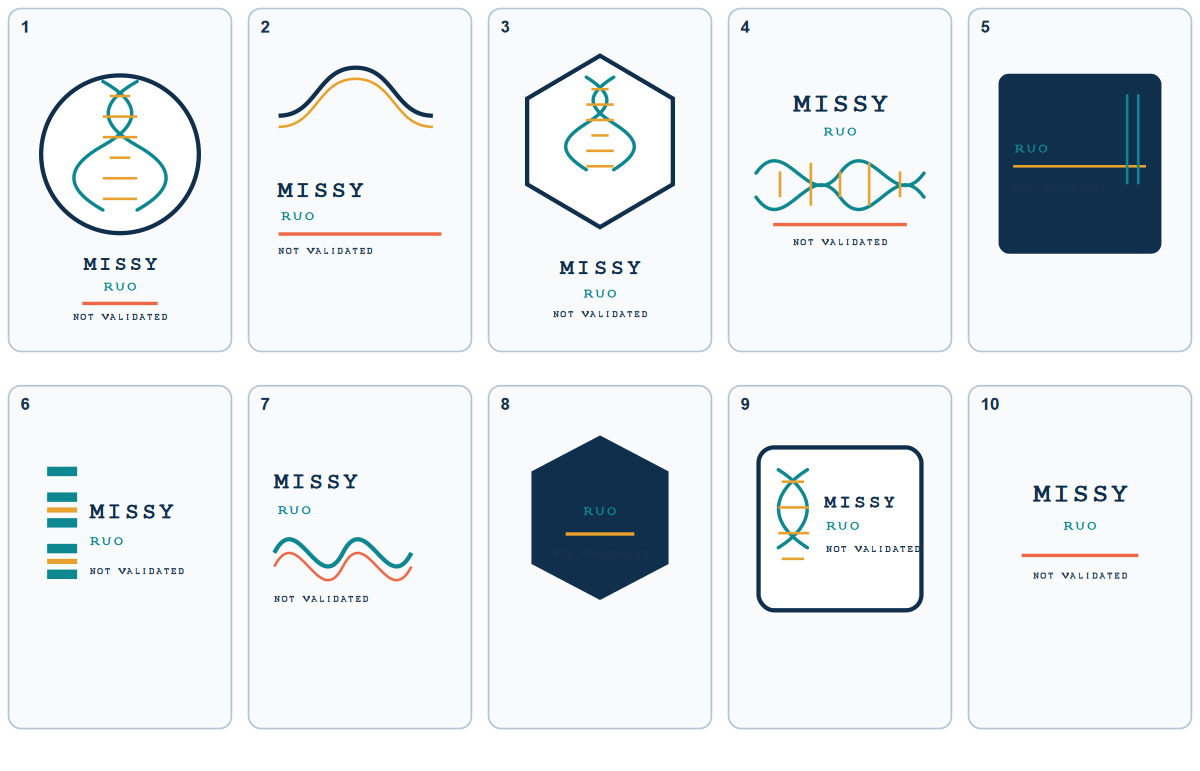
\includegraphics[width=0.96\textwidth]{fig/missy_logo_options.png}
\caption{Ten deterministic logo choices. Option 3 is used by the build.}\label{fig:missy-options}
\end{figure}

\begin{figure}[htbp]\centering

\includegraphics[height=5cm]{fig/missy_option3_full.png}
\caption{Selected option 3 mark.}\label{fig:missy-option3}
\end{figure}

\section{Report cover and footer}
Metadata values are wrapped to the report text width. A list of run names is one value per line; the PDF writer advances the cursor once per line. Every generated report page has a footer with the mark and the page count.

\begin{itemize}
  \item Stored Cq values and calls are not rewritten.
  \item Profile laboratory and analyst fields are included in the report metadata and profile hash.
  \item The footer reserves a 24 point lower band.
\end{itemize}

\section{Catalogue}
The current catalogue contains 25 graph figures, 18 data tables and 58 individual control-chart figures: 101 concrete items. The selectors \texttt{cc:all}, \texttt{cc:hardware}, \texttt{cc:software}, \texttt{cc:method} and \texttt{cc:operator} expand to the relevant chart items. The same item builders supply assisted mode, command mode, PDF and ZIP output.

\begin{longtable}{@{}p{3.1cm}p{4.0cm}p{7.0cm}@{}}
\toprule Identifier & Kind & Options \\\midrule\endfirsthead
\toprule Identifier & Kind & Options \\\midrule\endhead
\texttt{img:*} & figure & target, metric, signal, log, colourby, level, control \\
\texttt{data:*} & table & run, rows, pseudo \\
\texttt{rec:*} & table & run, rows, pseudo \\
\texttt{cc:*} & figure & type, x, phase1, lambda, L, k, h, specLo, specHi, warnAhead, charts \\
\bottomrule
\end{longtable}

\section{Command grammar}
\begin{itemize}
  \item \texttt{select pattern key=value}: validate all options, then add the selection.
  \item \texttt{set pattern key=value}: validate all options, then update selected items.
  \item \texttt{show pattern}: print options in force.
  \item \texttt{reset pattern}: remove options and use defaults.
  \item \texttt{cc:all} and group selectors expand without changing chart calculations.
\end{itemize}

\section{Implemented source}
The following listings are extracted from the production HTML snapshot. The black background is intentional for code readability; line numbers are HTML line numbers.

\vhead{Option-3 mark and SVG placement}
\lstinputlisting[firstnumber=11006,numbers=left,language=JavaScript]{code/missy_option3.js}

\vhead{Catalogue schema}
\lstinputlisting[firstnumber=11216,numbers=left,language=JavaScript]{code/missy_schema.js}

\vhead{Control-chart catalogue adapter}
\lstinputlisting[firstnumber=11270,numbers=left,language=JavaScript]{code/missy_chart_items.js}

\vhead{Option validation and command actions}
\lstinputlisting[firstnumber=11505,numbers=left,language=JavaScript]{code/missy_commands.js}

\vhead{Report cover and page generation}
\lstinputlisting[firstnumber=11424,numbers=left,language=JavaScript]{code/missy_report.js}

\begin{figure}[htbp]\centering

\includegraphics[width=0.96\textwidth]{fig/dna_separator.png}
\caption{DNA separator used between major document parts.}\label{fig:dna-separator}
\end{figure}



\chapter{How every function in the page was validated}\label{ch:val-method}

An earlier validation record was questioned on one point, and the objection was
fair: the inputs were supplied by the same work that wrote the code, so a table of
passes proved only that the code agreed with its own fixtures. This chapter and
the two that follow answer that objection in the only way it can be answered ---
by printing, for every function and constant in the page, the input, where that
input came from, the code as it stands, and the output. A reader who doubts a
verdict can re-derive it without trusting the harness.

\section{What was under test}

{\small
\begin{longtable}{@{}ll@{}}
\toprule \textbf{Item} & \textbf{Value} \\\midrule\endfirsthead
\toprule \textbf{Item} & \textbf{Value} \\\midrule\endhead
\texttt{page} & \texttt{qpcr\_qc\_forensics.html (identical copy index.html)} \\
\texttt{SHA-256} & \texttt{5685e516afeee0b7f3af4d13f15ac25131b3d89d18ee508a3ec006105a14…} \\
\texttt{size} & \texttt{893,995 bytes} \\
\texttt{captured} & \texttt{2026-09-24 12:06:13 UTC} \\
\texttt{symbols indexed} & \texttt{676} \\
\bottomrule
\end{longtable}}


\section{The corpus}
Every file below was loaded through the page's own intake --- the same path an
operator uses. Nothing was edited and no value was placed into the model by hand.
The files are instrument and exchange files produced by ordinary demonstration
experiments; they are identified here by what they contain and by their checksum,
not by their origin.

{\small
\begin{longtable}{@{}lrl@{}}
\caption{The corpus the whole of this part was measured on.}\label{tab:val-corpus} \\
\toprule \textbf{File} & \textbf{Bytes} & \textbf{SHA-256 (first 24)} \\\midrule\endfirsthead
\toprule \textbf{File} & \textbf{Bytes} & \textbf{SHA-256 (first 24)} \\\midrule\endhead
\texttt{MULTIPLEX-4CH.eds} & 2,376,494 & \texttt{8e65cbd6585d5caf70d14778} \\
\texttt{ABSQUANT-DEMO.ixo} & 4,636,210 & \texttt{e820f46933485d5a4a1c94b9} \\
\texttt{PLATE-384.eds} & 2,869,499 & \texttt{b2da31fbc0c0cda4d175529a} \\
\texttt{example\_2\_tm\_annotated.rdml} & 252,547 & \texttt{e018dbad7ec4071af8825439} \\
\bottomrule
\end{longtable}}


Reading them produced 0 runs and 0 stored results, with no page error.

\section{Provenance classes}
Every argument carries one of four classes. The class says where the value came
from, so a verdict can be weighed: a function exercised only on class~S input has
been shown to run, not to be right on laboratory data.

{\small
\begin{longtable}{@{}llr@{}}
\toprule \textbf{Class} & \textbf{Meaning} & \textbf{Arguments} \\\midrule\endfirsthead
\toprule \textbf{Class} & \textbf{Meaning} & \textbf{Arguments} \\\midrule\endhead
\texttt{R} & a real instrument or exchange file, unmodified, decoded by the page i… & 140 \\
\texttt{D} & derived by the code under test from a real file & 76 \\
\texttt{S} & synthetic, written for this probe & 336 \\
\texttt{E} & the live interface of the page after the corpus was loaded & 23 \\
\bottomrule
\end{longtable}}


\section{The three passes}
A probe that changes application state poisons every probe after it, so the
capture runs three times.

{\small
\begin{longtable}{@{}ll@{}}
\toprule \textbf{Pass} & \textbf{What it does} \\\midrule\endfirsthead
\toprule \textbf{Pass} & \textbf{What it does} \\\midrule\endhead
A, discovery & probe every symbol once; record which probes changed global state \\
B, clean & probe again in a new page with those names held back \\
C, isolation & probe each state-changing name in a page of its own \\
\bottomrule
\end{longtable}}


The delivered records are B plus C. One name, \vfn{renderPanel}, is state-changing
in pass~A and clean in pass~C: it had been disturbed by an earlier probe, not by
itself. That is the whole reason the three passes exist.

\section{What a verdict means}

{\small
\begin{longtable}{@{}llr@{}}
\toprule \textbf{Verdict} & \textbf{Meaning} & \textbf{Symbols} \\\midrule\endfirsthead
\toprule \textbf{Verdict} & \textbf{Meaning} & \textbf{Symbols} \\\midrule\endhead
\texttt{pass} & called with the stated input; returned the value shown; global state … & 527 \\
\texttt{const} & a declared value; its content at run time is shown & 113 \\
\texttt{priv} & declared inside a module closure; exercised through its module & 25 \\
\texttt{state} & changes application state; probed in a page of its own & 7 \\
\texttt{excl} & deliberately not called & 4 \\
\bottomrule
\end{longtable}}


\begin{notebox}[title={\textbf{What this part does not claim}}]
A pass means the function was called with the stated input and returned the stated
value without disturbing the application. It is a recorded behaviour, not a proof
of correctness. Correctness is argued in Chapter~\ref{ch:val-oracles}, by
properties that must hold of the values whatever produced them, and by inputs
whose right answer was fixed before the page saw them.
\end{notebox}

\section{Coverage}
The index is built from the page's own script: every top-level declaration is
probed, and the members of the one module that hides its helpers are probed
through the module. It contains 676 symbols. The index that shipped with the
previous release of this document was built by a parser that walked only the
outermost level and recorded 579; the difference is 97 symbols, most of them
module-level bindings and the helpers inside that module.

Of the 676, 527 functions executed and 113 constants were read --- 640 symbols with a
recorded input and output. 25 are declared inside a module closure. 4 are
deliberately not called, each with its reason. 7 change application state by
design and were probed in isolation. 0 raised an error.


\chapter{Function and constant source index}
\label{ch:val-functions}

This chapter lists every indexed top-level function, object, array and callable constant in declaration order. Each entry contains the exact source range from the current HTML build. The source listing is the test input for the corresponding symbol.

\subsection*{\texttt{\detokenize{ZH_TERMS}}}
\label{vf_1_ZH_TERMS}
HTML lines 996--1920. Kind: ObjectExpression.
\vhead{Source as built}
\lstinputlisting[firstnumber=996,numbers=left,language=JavaScript]{code/indexed/0001_ZH_TERMS.js}
\vhead{Validation record}
Input: page state and arguments used by the function.
Output: return value or state effect recorded by the harness.
Verdict: source range present in the current build.

\subsection*{\texttt{\detokenize{zhPhrase}}}
\label{vf_2_zhPhrase}
HTML lines 1924--2002. Kind: function.
\vhead{Source as built}
\lstinputlisting[firstnumber=1924,numbers=left,language=JavaScript]{code/indexed/0002_zhPhrase.js}
\vhead{Validation record}
Input: page state and arguments used by the function.
Output: return value or state effect recorded by the harness.
Verdict: source range present in the current build.

\subsection*{\texttt{\detokenize{ui}}}
\label{vf_3_ui}
HTML lines 2003--2003. Kind: function.
\vhead{Source as built}
\lstinputlisting[firstnumber=2003,numbers=left,language=JavaScript]{code/indexed/0003_ui.js}
\vhead{Validation record}
Input: page state and arguments used by the function.
Output: return value or state effect recorded by the harness.
Verdict: source range present in the current build.

\subsection*{\texttt{\detokenize{localizeDOM}}}
\label{vf_4_localizeDOM}
HTML lines 2004--2023. Kind: function.
\vhead{Source as built}
\lstinputlisting[firstnumber=2004,numbers=left,language=JavaScript]{code/indexed/0004_localizeDOM.js}
\vhead{Validation record}
Input: page state and arguments used by the function.
Output: return value or state effect recorded by the harness.
Verdict: source range present in the current build.

\subsection*{\texttt{\detokenize{showCuteToast}}}
\label{vf_5_showCuteToast}
HTML lines 2024--2030. Kind: function.
\vhead{Source as built}
\lstinputlisting[firstnumber=2024,numbers=left,language=JavaScript]{code/indexed/0005_showCuteToast.js}
\vhead{Validation record}
Input: page state and arguments used by the function.
Output: return value or state effect recorded by the harness.
Verdict: source range present in the current build.

\subsection*{\texttt{\detokenize{languageStorageKey}}}
\label{vf_6_languageStorageKey}
HTML lines 2031--2031. Kind: function.
\vhead{Source as built}
\lstinputlisting[firstnumber=2031,numbers=left,language=JavaScript]{code/indexed/0006_languageStorageKey.js}
\vhead{Validation record}
Input: page state and arguments used by the function.
Output: return value or state effect recorded by the harness.
Verdict: source range present in the current build.

\subsection*{\texttt{\detokenize{rememberedLanguage}}}
\label{vf_7_rememberedLanguage}
HTML lines 2032--2032. Kind: function.
\vhead{Source as built}
\lstinputlisting[firstnumber=2032,numbers=left,language=JavaScript]{code/indexed/0007_rememberedLanguage.js}
\vhead{Validation record}
Input: page state and arguments used by the function.
Output: return value or state effect recorded by the harness.
Verdict: source range present in the current build.

\subsection*{\texttt{\detokenize{setLanguage}}}
\label{vf_8_setLanguage}
HTML lines 2033--2043. Kind: function.
\vhead{Source as built}
\lstinputlisting[firstnumber=2033,numbers=left,language=JavaScript]{code/indexed/0008_setLanguage.js}
\vhead{Validation record}
Input: page state and arguments used by the function.
Output: return value or state effect recorded by the harness.
Verdict: source range present in the current build.

\subsection*{\texttt{\detokenize{ROLES}}}
\label{vf_9_ROLES}
HTML lines 2045--2045. Kind: ArrayExpression.
\vhead{Source as built}
\lstinputlisting[firstnumber=2045,numbers=left,language=JavaScript]{code/indexed/0009_ROLES.js}
\vhead{Validation record}
Input: page state and arguments used by the function.
Output: return value or state effect recorded by the harness.
Verdict: source range present in the current build.

\subsection*{\texttt{\detokenize{REP_REGEX}}}
\label{vf_10_REP_REGEX}
HTML lines 2046--2050. Kind: ObjectExpression.
\vhead{Source as built}
\lstinputlisting[firstnumber=2046,numbers=left,language=JavaScript]{code/indexed/0010_REP_REGEX.js}
\vhead{Validation record}
Input: page state and arguments used by the function.
Output: return value or state effect recorded by the harness.
Verdict: source range present in the current build.

\subsection*{\texttt{\detokenize{CALL}}}
\label{vf_11_CALL}
HTML lines 2052--2052. Kind: ObjectExpression.
\vhead{Source as built}
\lstinputlisting[firstnumber=2052,numbers=left,language=JavaScript]{code/indexed/0011_CALL.js}
\vhead{Validation record}
Input: page state and arguments used by the function.
Output: return value or state effect recorded by the harness.
Verdict: source range present in the current build.

\subsection*{\texttt{\detokenize{SAMPLE_TYPE}}}
\label{vf_12_SAMPLE_TYPE}
HTML lines 2053--2057. Kind: ObjectExpression.
\vhead{Source as built}
\lstinputlisting[firstnumber=2053,numbers=left,language=JavaScript]{code/indexed/0012_SAMPLE_TYPE.js}
\vhead{Validation record}
Input: page state and arguments used by the function.
Output: return value or state effect recorded by the harness.
Verdict: source range present in the current build.

\subsection*{\texttt{\detokenize{TYPE_TO_ROLE}}}
\label{vf_13_TYPE_TO_ROLE}
HTML lines 2058--2062. Kind: ObjectExpression.
\vhead{Source as built}
\lstinputlisting[firstnumber=2058,numbers=left,language=JavaScript]{code/indexed/0013_TYPE_TO_ROLE.js}
\vhead{Validation record}
Input: page state and arguments used by the function.
Output: return value or state effect recorded by the harness.
Verdict: source range present in the current build.

\subsection*{\texttt{\detokenize{NEGATIVE_FAMILY}}}
\label{vf_14_NEGATIVE_FAMILY}
HTML lines 2063--2063. Kind: ArrayExpression.
\vhead{Source as built}
\lstinputlisting[firstnumber=2063,numbers=left,language=JavaScript]{code/indexed/0014_NEGATIVE_FAMILY.js}
\vhead{Validation record}
Input: page state and arguments used by the function.
Output: return value or state effect recorded by the harness.
Verdict: source range present in the current build.

\subsection*{\texttt{\detokenize{ROLE_COLOURS}}}
\label{vf_15_ROLE_COLOURS}
HTML lines 2064--2065. Kind: ObjectExpression.
\vhead{Source as built}
\lstinputlisting[firstnumber=2064,numbers=left,language=JavaScript]{code/indexed/0015_ROLE_COLOURS.js}
\vhead{Validation record}
Input: page state and arguments used by the function.
Output: return value or state effect recorded by the harness.
Verdict: source range present in the current build.

\subsection*{\texttt{\detokenize{ROLE_LINE}}}
\label{vf_16_ROLE_LINE}
HTML lines 2066--2067. Kind: ObjectExpression.
\vhead{Source as built}
\lstinputlisting[firstnumber=2066,numbers=left,language=JavaScript]{code/indexed/0016_ROLE_LINE.js}
\vhead{Validation record}
Input: page state and arguments used by the function.
Output: return value or state effect recorded by the harness.
Verdict: source range present in the current build.

\subsection*{\texttt{\detokenize{PALETTE}}}
\label{vf_17_PALETTE}
HTML lines 2068--2068. Kind: ArrayExpression.
\vhead{Source as built}
\lstinputlisting[firstnumber=2068,numbers=left,language=JavaScript]{code/indexed/0017_PALETTE.js}
\vhead{Validation record}
Input: page state and arguments used by the function.
Output: return value or state effect recorded by the harness.
Verdict: source range present in the current build.

\subsection*{\texttt{\detokenize{ce}}}
\label{vf_18_ce}
HTML lines 2070--2070. Kind: ArrowFunctionExpression.
\vhead{Source as built}
\lstinputlisting[firstnumber=2070,numbers=left,language=JavaScript]{code/indexed/0018_ce.js}
\vhead{Validation record}
Input: page state and arguments used by the function.
Output: return value or state effect recorded by the harness.
Verdict: source range present in the current build.

\subsection*{\texttt{\detokenize{clone}}}
\label{vf_19_clone}
HTML lines 2077--2077. Kind: function.
\vhead{Source as built}
\lstinputlisting[firstnumber=2077,numbers=left,language=JavaScript]{code/indexed/0019_clone.js}
\vhead{Validation record}
Input: page state and arguments used by the function.
Output: return value or state effect recorded by the harness.
Verdict: source range present in the current build.

\subsection*{\texttt{\detokenize{esc}}}
\label{vf_20_esc}
HTML lines 2078--2078. Kind: function.
\vhead{Source as built}
\lstinputlisting[firstnumber=2078,numbers=left,language=JavaScript]{code/indexed/0020_esc.js}
\vhead{Validation record}
Input: page state and arguments used by the function.
Output: return value or state effect recorded by the harness.
Verdict: source range present in the current build.

\subsection*{\texttt{\detokenize{xesc}}}
\label{vf_21_xesc}
HTML lines 2079--2079. Kind: function.
\vhead{Source as built}
\lstinputlisting[firstnumber=2079,numbers=left,language=JavaScript]{code/indexed/0021_xesc.js}
\vhead{Validation record}
Input: page state and arguments used by the function.
Output: return value or state effect recorded by the harness.
Verdict: source range present in the current build.

\subsection*{\texttt{\detokenize{safeName}}}
\label{vf_22_safeName}
HTML lines 2080--2080. Kind: function.
\vhead{Source as built}
\lstinputlisting[firstnumber=2080,numbers=left,language=JavaScript]{code/indexed/0022_safeName.js}
\vhead{Validation record}
Input: page state and arguments used by the function.
Output: return value or state effect recorded by the harness.
Verdict: source range present in the current build.

\subsection*{\texttt{\detokenize{bytesFrom}}}
\label{vf_23_bytesFrom}
HTML lines 2081--2081. Kind: function.
\vhead{Source as built}
\lstinputlisting[firstnumber=2081,numbers=left,language=JavaScript]{code/indexed/0023_bytesFrom.js}
\vhead{Validation record}
Input: page state and arguments used by the function.
Output: return value or state effect recorded by the harness.
Verdict: source range present in the current build.

\subsection*{\texttt{\detokenize{scrollToEl}}}
\label{vf_24_scrollToEl}
HTML lines 2082--2082. Kind: function.
\vhead{Source as built}
\lstinputlisting[firstnumber=2082,numbers=left,language=JavaScript]{code/indexed/0024_scrollToEl.js}
\vhead{Validation record}
Input: page state and arguments used by the function.
Output: return value or state effect recorded by the harness.
Verdict: source range present in the current build.

\subsection*{\texttt{\detokenize{option}}}
\label{vf_25_option}
HTML lines 2083--2083. Kind: function.
\vhead{Source as built}
\lstinputlisting[firstnumber=2083,numbers=left,language=JavaScript]{code/indexed/0025_option.js}
\vhead{Validation record}
Input: page state and arguments used by the function.
Output: return value or state effect recorded by the harness.
Verdict: source range present in the current build.

\subsection*{\texttt{\detokenize{num}}}
\label{vf_26_num}
HTML lines 2084--2084. Kind: function.
\vhead{Source as built}
\lstinputlisting[firstnumber=2084,numbers=left,language=JavaScript]{code/indexed/0026_num.js}
\vhead{Validation record}
Input: page state and arguments used by the function.
Output: return value or state effect recorded by the harness.
Verdict: source range present in the current build.

\subsection*{\texttt{\detokenize{safeRe}}}
\label{vf_27_safeRe}
HTML lines 2085--2085. Kind: function.
\vhead{Source as built}
\lstinputlisting[firstnumber=2085,numbers=left,language=JavaScript]{code/indexed/0027_safeRe.js}
\vhead{Validation record}
Input: page state and arguments used by the function.
Output: return value or state effect recorded by the harness.
Verdict: source range present in the current build.

\subsection*{\texttt{\detokenize{uniq}}}
\label{vf_28_uniq}
HTML lines 2086--2086. Kind: function.
\vhead{Source as built}
\lstinputlisting[firstnumber=2086,numbers=left,language=JavaScript]{code/indexed/0028_uniq.js}
\vhead{Validation record}
Input: page state and arguments used by the function.
Output: return value or state effect recorded by the harness.
Verdict: source range present in the current build.

\subsection*{\texttt{\detokenize{byKey}}}
\label{vf_29_byKey}
HTML lines 2087--2087. Kind: function.
\vhead{Source as built}
\lstinputlisting[firstnumber=2087,numbers=left,language=JavaScript]{code/indexed/0029_byKey.js}
\vhead{Validation record}
Input: page state and arguments used by the function.
Output: return value or state effect recorded by the harness.
Verdict: source range present in the current build.

\subsection*{\texttt{\detokenize{mean}}}
\label{vf_30_mean}
HTML lines 2092--2092. Kind: function.
\vhead{Source as built}
\lstinputlisting[firstnumber=2092,numbers=left,language=JavaScript]{code/indexed/0030_mean.js}
\vhead{Validation record}
Input: page state and arguments used by the function.
Output: return value or state effect recorded by the harness.
Verdict: source range present in the current build.

\subsection*{\texttt{\detokenize{sd}}}
\label{vf_31_sd}
HTML lines 2094--2094. Kind: function.
\vhead{Source as built}
\lstinputlisting[firstnumber=2094,numbers=left,language=JavaScript]{code/indexed/0031_sd.js}
\vhead{Validation record}
Input: page state and arguments used by the function.
Output: return value or state effect recorded by the harness.
Verdict: source range present in the current build.

\subsection*{\texttt{\detokenize{median}}}
\label{vf_32_median}
HTML lines 2095--2095. Kind: function.
\vhead{Source as built}
\lstinputlisting[firstnumber=2095,numbers=left,language=JavaScript]{code/indexed/0032_median.js}
\vhead{Validation record}
Input: page state and arguments used by the function.
Output: return value or state effect recorded by the harness.
Verdict: source range present in the current build.

\subsection*{\texttt{\detokenize{percentile}}}
\label{vf_33_percentile}
HTML lines 2097--2102. Kind: function.
\vhead{Source as built}
\lstinputlisting[firstnumber=2097,numbers=left,language=JavaScript]{code/indexed/0033_percentile.js}
\vhead{Validation record}
Input: page state and arguments used by the function.
Output: return value or state effect recorded by the harness.
Verdict: source range present in the current build.

\subsection*{\texttt{\detokenize{range}}}
\label{vf_34_range}
HTML lines 2103--2103. Kind: function.
\vhead{Source as built}
\lstinputlisting[firstnumber=2103,numbers=left,language=JavaScript]{code/indexed/0034_range.js}
\vhead{Validation record}
Input: page state and arguments used by the function.
Output: return value or state effect recorded by the harness.
Verdict: source range present in the current build.

\subsection*{\texttt{\detokenize{cv}}}
\label{vf_35_cv}
HTML lines 2104--2104. Kind: function.
\vhead{Source as built}
\lstinputlisting[firstnumber=2104,numbers=left,language=JavaScript]{code/indexed/0035_cv.js}
\vhead{Validation record}
Input: page state and arguments used by the function.
Output: return value or state effect recorded by the harness.
Verdict: source range present in the current build.

\subsection*{\texttt{\detokenize{lgamma}}}
\label{vf_36_lgamma}
HTML lines 2107--2112. Kind: function.
\vhead{Source as built}
\lstinputlisting[firstnumber=2107,numbers=left,language=JavaScript]{code/indexed/0036_lgamma.js}
\vhead{Validation record}
Input: page state and arguments used by the function.
Output: return value or state effect recorded by the harness.
Verdict: source range present in the current build.

\subsection*{\texttt{\detokenize{betacf}}}
\label{vf_37_betacf}
HTML lines 2114--2133. Kind: function.
\vhead{Source as built}
\lstinputlisting[firstnumber=2114,numbers=left,language=JavaScript]{code/indexed/0037_betacf.js}
\vhead{Validation record}
Input: page state and arguments used by the function.
Output: return value or state effect recorded by the harness.
Verdict: source range present in the current build.

\subsection*{\texttt{\detokenize{betai}}}
\label{vf_38_betai}
HTML lines 2134--2138. Kind: function.
\vhead{Source as built}
\lstinputlisting[firstnumber=2134,numbers=left,language=JavaScript]{code/indexed/0038_betai.js}
\vhead{Validation record}
Input: page state and arguments used by the function.
Output: return value or state effect recorded by the harness.
Verdict: source range present in the current build.

\subsection*{\texttt{\detokenize{tDistTwoTail}}}
\label{vf_39_tDistTwoTail}
HTML lines 2140--2143. Kind: function.
\vhead{Source as built}
\lstinputlisting[firstnumber=2140,numbers=left,language=JavaScript]{code/indexed/0039_tDistTwoTail.js}
\vhead{Validation record}
Input: page state and arguments used by the function.
Output: return value or state effect recorded by the harness.
Verdict: source range present in the current build.

\subsection*{\texttt{\detokenize{gammap}}}
\label{vf_40_gammap}
HTML lines 2145--2160. Kind: function.
\vhead{Source as built}
\lstinputlisting[firstnumber=2145,numbers=left,language=JavaScript]{code/indexed/0040_gammap.js}
\vhead{Validation record}
Input: page state and arguments used by the function.
Output: return value or state effect recorded by the harness.
Verdict: source range present in the current build.

\subsection*{\texttt{\detokenize{chiSqP}}}
\label{vf_41_chiSqP}
HTML lines 2161--2161. Kind: function.
\vhead{Source as built}
\lstinputlisting[firstnumber=2161,numbers=left,language=JavaScript]{code/indexed/0041_chiSqP.js}
\vhead{Validation record}
Input: page state and arguments used by the function.
Output: return value or state effect recorded by the harness.
Verdict: source range present in the current build.

\subsection*{\texttt{\detokenize{tTest}}}
\label{vf_42_tTest}
HTML lines 2164--2187. Kind: function.
\vhead{Source as built}
\lstinputlisting[firstnumber=2164,numbers=left,language=JavaScript]{code/indexed/0042_tTest.js}
\vhead{Validation record}
Input: page state and arguments used by the function.
Output: return value or state effect recorded by the harness.
Verdict: source range present in the current build.

\subsection*{\texttt{\detokenize{fitLin}}}
\label{vf_43_fitLin}
HTML lines 2188--2195. Kind: function.
\vhead{Source as built}
\lstinputlisting[firstnumber=2188,numbers=left,language=JavaScript]{code/indexed/0043_fitLin.js}
\vhead{Validation record}
Input: page state and arguments used by the function.
Output: return value or state effect recorded by the harness.
Verdict: source range present in the current build.

\subsection*{\texttt{\detokenize{CRC_TABLE}}}
\label{vf_44_CRC_TABLE}
HTML lines 2200--2200. Kind: CallExpression.
\vhead{Source as built}
\lstinputlisting[firstnumber=2200,numbers=left,language=JavaScript]{code/indexed/0044_CRC_TABLE.js}
\vhead{Validation record}
Input: page state and arguments used by the function.
Output: return value or state effect recorded by the harness.
Verdict: source range present in the current build.

\subsection*{\texttt{\detokenize{crc32}}}
\label{vf_45_crc32}
HTML lines 2201--2201. Kind: function.
\vhead{Source as built}
\lstinputlisting[firstnumber=2201,numbers=left,language=JavaScript]{code/indexed/0045_crc32.js}
\vhead{Validation record}
Input: page state and arguments used by the function.
Output: return value or state effect recorded by the harness.
Verdict: source range present in the current build.

\subsection*{\texttt{\detokenize{sourceSha256}}}
\label{vf_46_sourceSha256}
HTML lines 2206--2212. Kind: function.
\vhead{Source as built}
\lstinputlisting[firstnumber=2206,numbers=left,language=JavaScript]{code/indexed/0046_sourceSha256.js}
\vhead{Validation record}
Input: page state and arguments used by the function.
Output: return value or state effect recorded by the harness.
Verdict: source range present in the current build.

\subsection*{\texttt{\detokenize{sha256Hex}}}
\label{vf_47_sha256Hex}
HTML lines 2213--2245. Kind: function.
\vhead{Source as built}
\lstinputlisting[firstnumber=2213,numbers=left,language=JavaScript]{code/indexed/0047_sha256Hex.js}
\vhead{Validation record}
Input: page state and arguments used by the function.
Output: return value or state effect recorded by the harness.
Verdict: source range present in the current build.

\subsection*{\texttt{\detokenize{inflate}}}
\label{vf_48_inflate}
HTML lines 2246--2251. Kind: function.
\vhead{Source as built}
\lstinputlisting[firstnumber=2246,numbers=left,language=JavaScript]{code/indexed/0048_inflate.js}
\vhead{Validation record}
Input: page state and arguments used by the function.
Output: return value or state effect recorded by the harness.
Verdict: source range present in the current build.

\subsection*{\texttt{\detokenize{readZip}}}
\label{vf_49_readZip}
HTML lines 2253--2278. Kind: function.
\vhead{Source as built}
\lstinputlisting[firstnumber=2253,numbers=left,language=JavaScript]{code/indexed/0049_readZip.js}
\vhead{Validation record}
Input: page state and arguments used by the function.
Output: return value or state effect recorded by the harness.
Verdict: source range present in the current build.

\subsection*{\texttt{\detokenize{dosStamp}}}
\label{vf_50_dosStamp}
HTML lines 2279--2283. Kind: function.
\vhead{Source as built}
\lstinputlisting[firstnumber=2279,numbers=left,language=JavaScript]{code/indexed/0050_dosStamp.js}
\vhead{Validation record}
Input: page state and arguments used by the function.
Output: return value or state effect recorded by the harness.
Verdict: source range present in the current build.

\subsection*{\texttt{\detokenize{makeStoredZip}}}
\label{vf_51_makeStoredZip}
HTML lines 2284--2309. Kind: function.
\vhead{Source as built}
\lstinputlisting[firstnumber=2284,numbers=left,language=JavaScript]{code/indexed/0051_makeStoredZip.js}
\vhead{Validation record}
Input: page state and arguments used by the function.
Output: return value or state effect recorded by the harness.
Verdict: source range present in the current build.

\subsection*{\texttt{\detokenize{propText}}}
\label{vf_52_propText}
HTML lines 2317--2317. Kind: function.
\vhead{Source as built}
\lstinputlisting[firstnumber=2317,numbers=left,language=JavaScript]{code/indexed/0052_propText.js}
\vhead{Validation record}
Input: page state and arguments used by the function.
Output: return value or state effect recorded by the harness.
Verdict: source range present in the current build.

\subsection*{\texttt{\detokenize{pv}}}
\label{vf_53_pv}
HTML lines 2318--2318. Kind: function.
\vhead{Source as built}
\lstinputlisting[firstnumber=2318,numbers=left,language=JavaScript]{code/indexed/0053_pv.js}
\vhead{Validation record}
Input: page state and arguments used by the function.
Output: return value or state effect recorded by the harness.
Verdict: source range present in the current build.

\subsection*{\texttt{\detokenize{propValues}}}
\label{vf_54_propValues}
HTML lines 2319--2319. Kind: function.
\vhead{Source as built}
\lstinputlisting[firstnumber=2319,numbers=left,language=JavaScript]{code/indexed/0054_propValues.js}
\vhead{Validation record}
Input: page state and arguments used by the function.
Output: return value or state effect recorded by the harness.
Verdict: source range present in the current build.

\subsection*{\texttt{\detokenize{base64ToBytes}}}
\label{vf_55_base64ToBytes}
HTML lines 2320--2320. Kind: function.
\vhead{Source as built}
\lstinputlisting[firstnumber=2320,numbers=left,language=JavaScript]{code/indexed/0055_base64ToBytes.js}
\vhead{Validation record}
Input: page state and arguments used by the function.
Output: return value or state effect recorded by the harness.
Verdict: source range present in the current build.

\subsection*{\texttt{\detokenize{posToWell}}}
\label{vf_56_posToWell}
HTML lines 2321--2321. Kind: function.
\vhead{Source as built}
\lstinputlisting[firstnumber=2321,numbers=left,language=JavaScript]{code/indexed/0056_posToWell.js}
\vhead{Validation record}
Input: page state and arguments used by the function.
Output: return value or state effect recorded by the harness.
Verdict: source range present in the current build.

\subsection*{\texttt{\detokenize{posToLimsWell}}}
\label{vf_57_posToLimsWell}
HTML lines 2322--2322. Kind: function.
\vhead{Source as built}
\lstinputlisting[firstnumber=2322,numbers=left,language=JavaScript]{code/indexed/0057_posToLimsWell.js}
\vhead{Validation record}
Input: page state and arguments used by the function.
Output: return value or state effect recorded by the harness.
Verdict: source range present in the current build.

\subsection*{\texttt{\detokenize{wellToPos}}}
\label{vf_58_wellToPos}
HTML lines 2323--2326. Kind: function.
\vhead{Source as built}
\lstinputlisting[firstnumber=2323,numbers=left,language=JavaScript]{code/indexed/0058_wellToPos.js}
\vhead{Validation record}
Input: page state and arguments used by the function.
Output: return value or state effect recorded by the harness.
Verdict: source range present in the current build.

\subsection*{\texttt{\detokenize{hexBEToDouble}}}
\label{vf_59_hexBEToDouble}
HTML lines 2327--2334. Kind: function.
\vhead{Source as built}
\lstinputlisting[firstnumber=2327,numbers=left,language=JavaScript]{code/indexed/0059_hexBEToDouble.js}
\vhead{Validation record}
Input: page state and arguments used by the function.
Output: return value or state effect recorded by the harness.
Verdict: source range present in the current build.

\subsection*{\texttt{\detokenize{decodeAcq}}}
\label{vf_60_decodeAcq}
HTML lines 2336--2423. Kind: function.
\vhead{Source as built}
\lstinputlisting[firstnumber=2336,numbers=left,language=JavaScript]{code/indexed/0060_decodeAcq.js}
\vhead{Validation record}
Input: page state and arguments used by the function.
Output: return value or state effect recorded by the harness.
Verdict: source range present in the current build.

\subsection*{\texttt{\detokenize{acquisitionStats}}}
\label{vf_61_acquisitionStats}
HTML lines 2424--2431. Kind: function.
\vhead{Source as built}
\lstinputlisting[firstnumber=2424,numbers=left,language=JavaScript]{code/indexed/0061_acquisitionStats.js}
\vhead{Validation record}
Input: page state and arguments used by the function.
Output: return value or state effect recorded by the harness.
Verdict: source range present in the current build.

\subsection*{\texttt{\detokenize{decodePlateModel}}}
\label{vf_62_decodePlateModel}
HTML lines 2434--2495. Kind: function.
\vhead{Source as built}
\lstinputlisting[firstnumber=2434,numbers=left,language=JavaScript]{code/indexed/0062_decodePlateModel.js}
\vhead{Validation record}
Input: page state and arguments used by the function.
Output: return value or state effect recorded by the harness.
Verdict: source range present in the current build.

\subsection*{\texttt{\detokenize{decodeSubsets}}}
\label{vf_63_decodeSubsets}
HTML lines 2497--2507. Kind: function.
\vhead{Source as built}
\lstinputlisting[firstnumber=2497,numbers=left,language=JavaScript]{code/indexed/0063_decodeSubsets.js}
\vhead{Validation record}
Input: page state and arguments used by the function.
Output: return value or state effect recorded by the harness.
Verdict: source range present in the current build.

\subsection*{\texttt{\detokenize{decodeProtocol}}}
\label{vf_64_decodeProtocol}
HTML lines 2509--2544. Kind: function.
\vhead{Source as built}
\lstinputlisting[firstnumber=2509,numbers=left,language=JavaScript]{code/indexed/0064_decodeProtocol.js}
\vhead{Validation record}
Input: page state and arguments used by the function.
Output: return value or state effect recorded by the harness.
Verdict: source range present in the current build.

\subsection*{\texttt{\detokenize{ANALYSIS_KINDS}}}
\label{vf_65_ANALYSIS_KINDS}
HTML lines 2552--2560. Kind: ArrayExpression.
\vhead{Source as built}
\lstinputlisting[firstnumber=2552,numbers=left,language=JavaScript]{code/indexed/0065_ANALYSIS_KINDS.js}
\vhead{Validation record}
Input: page state and arguments used by the function.
Output: return value or state effect recorded by the harness.
Verdict: source range present in the current build.

\subsection*{\texttt{\detokenize{analysisKind}}}
\label{vf_66_analysisKind}
HTML lines 2561--2565. Kind: function.
\vhead{Source as built}
\lstinputlisting[firstnumber=2561,numbers=left,language=JavaScript]{code/indexed/0066_analysisKind.js}
\vhead{Validation record}
Input: page state and arguments used by the function.
Output: return value or state effect recorded by the harness.
Verdict: source range present in the current build.

\subsection*{\texttt{\detokenize{LC_CALC_STATE_LABELS}}}
\label{vf_67_LC_CALC_STATE_LABELS}
HTML lines 2570--2570. Kind: ObjectExpression.
\vhead{Source as built}
\lstinputlisting[firstnumber=2570,numbers=left,language=JavaScript]{code/indexed/0067_LC_CALC_STATE_LABELS.js}
\vhead{Validation record}
Input: page state and arguments used by the function.
Output: return value or state effect recorded by the harness.
Verdict: source range present in the current build.

\subsection*{\texttt{\detokenize{calcStateLabel}}}
\label{vf_68_calcStateLabel}
HTML lines 2571--2571. Kind: function.
\vhead{Source as built}
\lstinputlisting[firstnumber=2571,numbers=left,language=JavaScript]{code/indexed/0068_calcStateLabel.js}
\vhead{Validation record}
Input: page state and arguments used by the function.
Output: return value or state effect recorded by the harness.
Verdict: source range present in the current build.

\subsection*{\texttt{\detokenize{cpMethodOf}}}
\label{vf_69_cpMethodOf}
HTML lines 2572--2578. Kind: function.
\vhead{Source as built}
\lstinputlisting[firstnumber=2572,numbers=left,language=JavaScript]{code/indexed/0069_cpMethodOf.js}
\vhead{Validation record}
Input: page state and arguments used by the function.
Output: return value or state effect recorded by the harness.
Verdict: source range present in the current build.

\subsection*{\texttt{\detokenize{RESULT_PROPS}}}
\label{vf_70_RESULT_PROPS}
HTML lines 2580--2581. Kind: ArrayExpression.
\vhead{Source as built}
\lstinputlisting[firstnumber=2580,numbers=left,language=JavaScript]{code/indexed/0070_RESULT_PROPS.js}
\vhead{Validation record}
Input: page state and arguments used by the function.
Output: return value or state effect recorded by the harness.
Verdict: source range present in the current build.

\subsection*{\texttt{\detokenize{readLists}}}
\label{vf_71_readLists}
HTML lines 2582--2590. Kind: function.
\vhead{Source as built}
\lstinputlisting[firstnumber=2582,numbers=left,language=JavaScript]{code/indexed/0071_readLists.js}
\vhead{Validation record}
Input: page state and arguments used by the function.
Output: return value or state effect recorded by the harness.
Verdict: source range present in the current build.

\subsection*{\texttt{\detokenize{resultKindOf}}}
\label{vf_72_resultKindOf}
HTML lines 2591--2601. Kind: function.
\vhead{Source as built}
\lstinputlisting[firstnumber=2591,numbers=left,language=JavaScript]{code/indexed/0072_resultKindOf.js}
\vhead{Validation record}
Input: page state and arguments used by the function.
Output: return value or state effect recorded by the harness.
Verdict: source range present in the current build.

\subsection*{\texttt{\detokenize{PAIRING_RULES}}}
\label{vf_73_PAIRING_RULES}
HTML lines 2608--2608. Kind: ObjectExpression.
\vhead{Source as built}
\lstinputlisting[firstnumber=2608,numbers=left,language=JavaScript]{code/indexed/0073_PAIRING_RULES.js}
\vhead{Validation record}
Input: page state and arguments used by the function.
Output: return value or state effect recorded by the harness.
Verdict: source range present in the current build.

\subsection*{\texttt{\detokenize{rqResult}}}
\label{vf_74_rqResult}
HTML lines 2609--2625. Kind: function.
\vhead{Source as built}
\lstinputlisting[firstnumber=2609,numbers=left,language=JavaScript]{code/indexed/0074_rqResult.js}
\vhead{Validation record}
Input: page state and arguments used by the function.
Output: return value or state effect recorded by the harness.
Verdict: source range present in the current build.

\subsection*{\texttt{\detokenize{decodeRelQuant}}}
\label{vf_75_decodeRelQuant}
HTML lines 2626--2672. Kind: function.
\vhead{Source as built}
\lstinputlisting[firstnumber=2626,numbers=left,language=JavaScript]{code/indexed/0075_decodeRelQuant.js}
\vhead{Validation record}
Input: page state and arguments used by the function.
Output: return value or state effect recorded by the harness.
Verdict: source range present in the current build.

\subsection*{\texttt{\detokenize{ownedBy}}}
\label{vf_76_ownedBy}
HTML lines 2677--2685. Kind: function.
\vhead{Source as built}
\lstinputlisting[firstnumber=2677,numbers=left,language=JavaScript]{code/indexed/0076_ownedBy.js}
\vhead{Validation record}
Input: page state and arguments used by the function.
Output: return value or state effect recorded by the harness.
Verdict: source range present in the current build.

\subsection*{\texttt{\detokenize{ownQueryAll}}}
\label{vf_77_ownQueryAll}
HTML lines 2686--2686. Kind: function.
\vhead{Source as built}
\lstinputlisting[firstnumber=2686,numbers=left,language=JavaScript]{code/indexed/0077_ownQueryAll.js}
\vhead{Validation record}
Input: page state and arguments used by the function.
Output: return value or state effect recorded by the harness.
Verdict: source range present in the current build.

\subsection*{\texttt{\detokenize{ownQuery}}}
\label{vf_78_ownQuery}
HTML lines 2687--2687. Kind: function.
\vhead{Source as built}
\lstinputlisting[firstnumber=2687,numbers=left,language=JavaScript]{code/indexed/0078_ownQuery.js}
\vhead{Validation record}
Input: page state and arguments used by the function.
Output: return value or state effect recorded by the harness.
Verdict: source range present in the current build.

\subsection*{\texttt{\detokenize{decodeAnalyses}}}
\label{vf_79_decodeAnalyses}
HTML lines 2689--2776. Kind: function.
\vhead{Source as built}
\lstinputlisting[firstnumber=2689,numbers=left,language=JavaScript]{code/indexed/0079_decodeAnalyses.js}
\vhead{Validation record}
Input: page state and arguments used by the function.
Output: return value or state effect recorded by the harness.
Verdict: source range present in the current build.

\subsection*{\texttt{\detokenize{ownsResult}}}
\label{vf_80_ownsResult}
HTML lines 2783--2791. Kind: function.
\vhead{Source as built}
\lstinputlisting[firstnumber=2783,numbers=left,language=JavaScript]{code/indexed/0080_ownsResult.js}
\vhead{Validation record}
Input: page state and arguments used by the function.
Output: return value or state effect recorded by the harness.
Verdict: source range present in the current build.

\subsection*{\texttt{\detokenize{analysisResults}}}
\label{vf_81_analysisResults}
HTML lines 2792--2811. Kind: function.
\vhead{Source as built}
\lstinputlisting[firstnumber=2792,numbers=left,language=JavaScript]{code/indexed/0081_analysisResults.js}
\vhead{Validation record}
Input: page state and arguments used by the function.
Output: return value or state effect recorded by the harness.
Verdict: source range present in the current build.

\subsection*{\texttt{\detokenize{decodeIxo}}}
\label{vf_82_decodeIxo}
HTML lines 2813--3155. Kind: function.
\vhead{Source as built}
\lstinputlisting[firstnumber=2813,numbers=left,language=JavaScript]{code/indexed/0082_decodeIxo.js}
\vhead{Validation record}
Input: page state and arguments used by the function.
Output: return value or state effect recorded by the harness.
Verdict: source range present in the current build.

\subsection*{\texttt{\detokenize{EDS}}}
\label{vf_83_EDS}
HTML lines 3160--3708. Kind: CallExpression.
\vhead{Source as built}
\lstinputlisting[firstnumber=3160,numbers=left,language=JavaScript]{code/indexed/0083_EDS.js}
\vhead{Validation record}
Input: page state and arguments used by the function.
Output: return value or state effect recorded by the harness.
Verdict: source range present in the current build.

\subsection*{\texttt{\detokenize{$}}}
\label{vf_84__}
HTML lines 3163--3163. Kind: ArrowFunctionExpression.
\vhead{Source as built}
\lstinputlisting[firstnumber=3163,numbers=left,language=JavaScript]{code/indexed/0084_.js}
\vhead{Validation record}
Input: page state and arguments used by the function.
Output: return value or state effect recorded by the harness.
Verdict: source range present in the current build.

\subsection*{\texttt{\detokenize{esc}}}
\label{vf_85_esc}
HTML lines 3164--3164. Kind: ArrowFunctionExpression.
\vhead{Source as built}
\lstinputlisting[firstnumber=3164,numbers=left,language=JavaScript]{code/indexed/0085_esc.js}
\vhead{Validation record}
Input: page state and arguments used by the function.
Output: return value or state effect recorded by the harness.
Verdict: source range present in the current build.

\subsection*{\texttt{\detokenize{num}}}
\label{vf_86_num}
HTML lines 3165--3165. Kind: ArrowFunctionExpression.
\vhead{Source as built}
\lstinputlisting[firstnumber=3165,numbers=left,language=JavaScript]{code/indexed/0086_num.js}
\vhead{Validation record}
Input: page state and arguments used by the function.
Output: return value or state effect recorded by the harness.
Verdict: source range present in the current build.

\subsection*{\texttt{\detokenize{fmt}}}
\label{vf_87_fmt}
HTML lines 3166--3166. Kind: ArrowFunctionExpression.
\vhead{Source as built}
\lstinputlisting[firstnumber=3166,numbers=left,language=JavaScript]{code/indexed/0087_fmt.js}
\vhead{Validation record}
Input: page state and arguments used by the function.
Output: return value or state effect recorded by the harness.
Verdict: source range present in the current build.

\subsection*{\texttt{\detokenize{pill}}}
\label{vf_88_pill}
HTML lines 3167--3167. Kind: ArrowFunctionExpression.
\vhead{Source as built}
\lstinputlisting[firstnumber=3167,numbers=left,language=JavaScript]{code/indexed/0088_pill.js}
\vhead{Validation record}
Input: page state and arguments used by the function.
Output: return value or state effect recorded by the harness.
Verdict: source range present in the current build.

\subsection*{\texttt{\detokenize{dt}}}
\label{vf_89_dt}
HTML lines 3168--3168. Kind: ArrowFunctionExpression.
\vhead{Source as built}
\lstinputlisting[firstnumber=3168,numbers=left,language=JavaScript]{code/indexed/0089_dt.js}
\vhead{Validation record}
Input: page state and arguments used by the function.
Output: return value or state effect recorded by the harness.
Verdict: source range present in the current build.

\subsection*{\texttt{\detokenize{hex}}}
\label{vf_90_hex}
HTML lines 3169--3169. Kind: ArrowFunctionExpression.
\vhead{Source as built}
\lstinputlisting[firstnumber=3169,numbers=left,language=JavaScript]{code/indexed/0090_hex.js}
\vhead{Validation record}
Input: page state and arguments used by the function.
Output: return value or state effect recorded by the harness.
Verdict: source range present in the current build.

\subsection*{\texttt{\detokenize{mean}}}
\label{vf_91_mean}
HTML lines 3170--3170. Kind: ArrowFunctionExpression.
\vhead{Source as built}
\lstinputlisting[firstnumber=3170,numbers=left,language=JavaScript]{code/indexed/0091_mean.js}
\vhead{Validation record}
Input: page state and arguments used by the function.
Output: return value or state effect recorded by the harness.
Verdict: source range present in the current build.

\subsection*{\texttt{\detokenize{sd}}}
\label{vf_92_sd}
HTML lines 3171--3171. Kind: ArrowFunctionExpression.
\vhead{Source as built}
\lstinputlisting[firstnumber=3171,numbers=left,language=JavaScript]{code/indexed/0092_sd.js}
\vhead{Validation record}
Input: page state and arguments used by the function.
Output: return value or state effect recorded by the harness.
Verdict: source range present in the current build.

\subsection*{\texttt{\detokenize{wellPos}}}
\label{vf_93_wellPos}
HTML lines 3173--3173. Kind: ArrowFunctionExpression.
\vhead{Source as built}
\lstinputlisting[firstnumber=3173,numbers=left,language=JavaScript]{code/indexed/0093_wellPos.js}
\vhead{Validation record}
Input: page state and arguments used by the function.
Output: return value or state effect recorded by the harness.
Verdict: source range present in the current build.

\subsection*{\texttt{\detokenize{download}}}
\label{vf_94_download}
HTML lines 3174--3178. Kind: function.
\vhead{Source as built}
\lstinputlisting[firstnumber=3174,numbers=left,language=JavaScript]{code/indexed/0094_download.js}
\vhead{Validation record}
Input: page state and arguments used by the function.
Output: return value or state effect recorded by the harness.
Verdict: source range present in the current build.

\subsection*{\texttt{\detokenize{safeName}}}
\label{vf_95_safeName}
HTML lines 3179--3179. Kind: ArrowFunctionExpression.
\vhead{Source as built}
\lstinputlisting[firstnumber=3179,numbers=left,language=JavaScript]{code/indexed/0095_safeName.js}
\vhead{Validation record}
Input: page state and arguments used by the function.
Output: return value or state effect recorded by the harness.
Verdict: source range present in the current build.

\subsection*{\texttt{\detokenize{CRC_T}}}
\label{vf_96_CRC_T}
HTML lines 3182--3182. Kind: CallExpression.
\vhead{Source as built}
\lstinputlisting[firstnumber=3182,numbers=left,language=JavaScript]{code/indexed/0096_CRC_T.js}
\vhead{Validation record}
Input: page state and arguments used by the function.
Output: return value or state effect recorded by the harness.
Verdict: source range present in the current build.

\subsection*{\texttt{\detokenize{crc32}}}
\label{vf_97_crc32}
HTML lines 3183--3183. Kind: function.
\vhead{Source as built}
\lstinputlisting[firstnumber=3183,numbers=left,language=JavaScript]{code/indexed/0097_crc32.js}
\vhead{Validation record}
Input: page state and arguments used by the function.
Output: return value or state effect recorded by the harness.
Verdict: source range present in the current build.

\subsection*{\texttt{\detokenize{MD5}}}
\label{vf_98_MD5}
HTML lines 3186--3213. Kind: function.
\vhead{Source as built}
\lstinputlisting[firstnumber=3186,numbers=left,language=JavaScript]{code/indexed/0098_MD5.js}
\vhead{Validation record}
Input: page state and arguments used by the function.
Output: return value or state effect recorded by the harness.
Verdict: source range present in the current build.

\subsection*{\texttt{\detokenize{inflateRaw}}}
\label{vf_99_inflateRaw}
HTML lines 3216--3221. Kind: function.
\vhead{Source as built}
\lstinputlisting[firstnumber=3216,numbers=left,language=JavaScript]{code/indexed/0099_inflateRaw.js}
\vhead{Validation record}
Input: page state and arguments used by the function.
Output: return value or state effect recorded by the harness.
Verdict: source range present in the current build.

\subsection*{\texttt{\detokenize{readZip}}}
\label{vf_100_readZip}
HTML lines 3222--3249. Kind: function.
\vhead{Source as built}
\lstinputlisting[firstnumber=3222,numbers=left,language=JavaScript]{code/indexed/0100_readZip.js}
\vhead{Validation record}
Input: page state and arguments used by the function.
Output: return value or state effect recorded by the harness.
Verdict: source range present in the current build.

\subsection*{\texttt{\detokenize{makeZip}}}
\label{vf_101_makeZip}
HTML lines 3252--3268. Kind: function.
\vhead{Source as built}
\lstinputlisting[firstnumber=3252,numbers=left,language=JavaScript]{code/indexed/0101_makeZip.js}
\vhead{Validation record}
Input: page state and arguments used by the function.
Output: return value or state effect recorded by the harness.
Verdict: source range present in the current build.

\subsection*{\texttt{\detokenize{xml}}}
\label{vf_102_xml}
HTML lines 3271--3271. Kind: ArrowFunctionExpression.
\vhead{Source as built}
\lstinputlisting[firstnumber=3271,numbers=left,language=JavaScript]{code/indexed/0102_xml.js}
\vhead{Validation record}
Input: page state and arguments used by the function.
Output: return value or state effect recorded by the harness.
Verdict: source range present in the current build.

\subsection*{\texttt{\detokenize{kid}}}
\label{vf_103_kid}
HTML lines 3272--3272. Kind: ArrowFunctionExpression.
\vhead{Source as built}
\lstinputlisting[firstnumber=3272,numbers=left,language=JavaScript]{code/indexed/0103_kid.js}
\vhead{Validation record}
Input: page state and arguments used by the function.
Output: return value or state effect recorded by the harness.
Verdict: source range present in the current build.

\subsection*{\texttt{\detokenize{kids}}}
\label{vf_104_kids}
HTML lines 3273--3273. Kind: ArrowFunctionExpression.
\vhead{Source as built}
\lstinputlisting[firstnumber=3273,numbers=left,language=JavaScript]{code/indexed/0104_kids.js}
\vhead{Validation record}
Input: page state and arguments used by the function.
Output: return value or state effect recorded by the harness.
Verdict: source range present in the current build.

\subsection*{\texttt{\detokenize{txt}}}
\label{vf_105_txt}
HTML lines 3274--3274. Kind: ArrowFunctionExpression.
\vhead{Source as built}
\lstinputlisting[firstnumber=3274,numbers=left,language=JavaScript]{code/indexed/0105_txt.js}
\vhead{Validation record}
Input: page state and arguments used by the function.
Output: return value or state effect recorded by the harness.
Verdict: source range present in the current build.

\subsection*{\texttt{\detokenize{argb}}}
\label{vf_106_argb}
HTML lines 3275--3275. Kind: ArrowFunctionExpression.
\vhead{Source as built}
\lstinputlisting[firstnumber=3275,numbers=left,language=JavaScript]{code/indexed/0106_argb.js}
\vhead{Validation record}
Input: page state and arguments used by the function.
Output: return value or state effect recorded by the harness.
Verdict: source range present in the current build.

\subsection*{\texttt{\detokenize{bracketList}}}
\label{vf_107_bracketList}
HTML lines 3276--3276. Kind: ArrowFunctionExpression.
\vhead{Source as built}
\lstinputlisting[firstnumber=3276,numbers=left,language=JavaScript]{code/indexed/0107_bracketList.js}
\vhead{Validation record}
Input: page state and arguments used by the function.
Output: return value or state effect recorded by the harness.
Verdict: source range present in the current build.

\subsection*{\texttt{\detokenize{ini}}}
\label{vf_108_ini}
HTML lines 3277--3279. Kind: function.
\vhead{Source as built}
\lstinputlisting[firstnumber=3277,numbers=left,language=JavaScript]{code/indexed/0108_ini.js}
\vhead{Validation record}
Input: page state and arguments used by the function.
Output: return value or state effect recorded by the harness.
Verdict: source range present in the current build.

\subsection*{\texttt{\detokenize{FLAGS}}}
\label{vf_109_FLAGS}
HTML lines 3284--3302. Kind: ObjectExpression.
\vhead{Source as built}
\lstinputlisting[firstnumber=3284,numbers=left,language=JavaScript]{code/indexed/0109_FLAGS.js}
\vhead{Validation record}
Input: page state and arguments used by the function.
Output: return value or state effect recorded by the harness.
Verdict: source range present in the current build.

\subsection*{\texttt{\detokenize{flagName}}}
\label{vf_110_flagName}
HTML lines 3303--3303. Kind: ArrowFunctionExpression.
\vhead{Source as built}
\lstinputlisting[firstnumber=3303,numbers=left,language=JavaScript]{code/indexed/0110_flagName.js}
\vhead{Validation record}
Input: page state and arguments used by the function.
Output: return value or state effect recorded by the harness.
Verdict: source range present in the current build.

\subsection*{\texttt{\detokenize{parseEds}}}
\label{vf_111_parseEds}
HTML lines 3307--3513. Kind: function.
\vhead{Source as built}
\lstinputlisting[firstnumber=3307,numbers=left,language=JavaScript]{code/indexed/0111_parseEds.js}
\vhead{Validation record}
Input: page state and arguments used by the function.
Output: return value or state effect recorded by the harness.
Verdict: source range present in the current build.

\subsection*{\texttt{\detokenize{recalcCt}}}
\label{vf_112_recalcCt}
HTML lines 3517--3521. Kind: function.
\vhead{Source as built}
\lstinputlisting[firstnumber=3517,numbers=left,language=JavaScript]{code/indexed/0112_recalcCt.js}
\vhead{Validation record}
Input: page state and arguments used by the function.
Output: return value or state effect recorded by the harness.
Verdict: source range present in the current build.

\subsection*{\texttt{\detokenize{parseLog}}}
\label{vf_113_parseLog}
HTML lines 3523--3539. Kind: function.
\vhead{Source as built}
\lstinputlisting[firstnumber=3523,numbers=left,language=JavaScript]{code/indexed/0113_parseLog.js}
\vhead{Validation record}
Input: page state and arguments used by the function.
Output: return value or state effect recorded by the harness.
Verdict: source range present in the current build.

\subsection*{\texttt{\detokenize{studyRows}}}
\label{vf_114_studyRows}
HTML lines 3541--3545. Kind: function.
\vhead{Source as built}
\lstinputlisting[firstnumber=3541,numbers=left,language=JavaScript]{code/indexed/0114_studyRows.js}
\vhead{Validation record}
Input: page state and arguments used by the function.
Output: return value or state effect recorded by the harness.
Verdict: source range present in the current build.

\subsection*{\texttt{\detokenize{QS_DEFAULT_COLS}}}
\label{vf_115_QS_DEFAULT_COLS}
HTML lines 3553--3559. Kind: ObjectExpression.
\vhead{Source as built}
\lstinputlisting[firstnumber=3553,numbers=left,language=JavaScript]{code/indexed/0115_QS_DEFAULT_COLS.js}
\vhead{Validation record}
Input: page state and arguments used by the function.
Output: return value or state effect recorded by the harness.
Verdict: source range present in the current build.

\subsection*{\texttt{\detokenize{qsCols}}}
\label{vf_116_qsCols}
HTML lines 3560--3565. Kind: function.
\vhead{Source as built}
\lstinputlisting[firstnumber=3560,numbers=left,language=JavaScript]{code/indexed/0116_qsCols.js}
\vhead{Validation record}
Input: page state and arguments used by the function.
Output: return value or state effect recorded by the harness.
Verdict: source range present in the current build.

\subsection*{\texttt{\detokenize{pad2}}}
\label{vf_117_pad2}
HTML lines 3566--3566. Kind: ArrowFunctionExpression.
\vhead{Source as built}
\lstinputlisting[firstnumber=3566,numbers=left,language=JavaScript]{code/indexed/0117_pad2.js}
\vhead{Validation record}
Input: page state and arguments used by the function.
Output: return value or state effect recorded by the harness.
Verdict: source range present in the current build.

\subsection*{\texttt{\detokenize{qsCalDate}}}
\label{vf_118_qsCalDate}
HTML lines 3567--3567. Kind: function.
\vhead{Source as built}
\lstinputlisting[firstnumber=3567,numbers=left,language=JavaScript]{code/indexed/0118_qsCalDate.js}
\vhead{Validation record}
Input: page state and arguments used by the function.
Output: return value or state effect recorded by the harness.
Verdict: source range present in the current build.

\subsection*{\texttt{\detokenize{qsStamp}}}
\label{vf_119_qsStamp}
HTML lines 3568--3572. Kind: function.
\vhead{Source as built}
\lstinputlisting[firstnumber=3568,numbers=left,language=JavaScript]{code/indexed/0119_qsStamp.js}
\vhead{Validation record}
Input: page state and arguments used by the function.
Output: return value or state effect recorded by the harness.
Verdict: source range present in the current build.

\subsection*{\texttt{\detokenize{qsRGB}}}
\label{vf_120_qsRGB}
HTML lines 3573--3573. Kind: ArrowFunctionExpression.
\vhead{Source as built}
\lstinputlisting[firstnumber=3573,numbers=left,language=JavaScript]{code/indexed/0120_qsRGB.js}
\vhead{Validation record}
Input: page state and arguments used by the function.
Output: return value or state effect recorded by the harness.
Verdict: source range present in the current build.

\subsection*{\texttt{\detokenize{qsInstrument}}}
\label{vf_121_qsInstrument}
HTML lines 3576--3587. Kind: function.
\vhead{Source as built}
\lstinputlisting[firstnumber=3576,numbers=left,language=JavaScript]{code/indexed/0121_qsInstrument.js}
\vhead{Validation record}
Input: page state and arguments used by the function.
Output: return value or state effect recorded by the harness.
Verdict: source range present in the current build.

\subsection*{\texttt{\detokenize{javaHashOrder}}}
\label{vf_122_javaHashOrder}
HTML lines 3589--3593. Kind: function.
\vhead{Source as built}
\lstinputlisting[firstnumber=3589,numbers=left,language=JavaScript]{code/indexed/0122_javaHashOrder.js}
\vhead{Validation record}
Input: page state and arguments used by the function.
Output: return value or state effect recorded by the harness.
Verdict: source range present in the current build.

\subsection*{\texttt{\detokenize{qsHeader}}}
\label{vf_123_qsHeader}
HTML lines 3594--3613. Kind: function.
\vhead{Source as built}
\lstinputlisting[firstnumber=3594,numbers=left,language=JavaScript]{code/indexed/0123_qsHeader.js}
\vhead{Validation record}
Input: page state and arguments used by the function.
Output: return value or state effect recorded by the harness.
Verdict: source range present in the current build.

\subsection*{\texttt{\detokenize{qsTables}}}
\label{vf_124_qsTables}
HTML lines 3614--3692. Kind: function.
\vhead{Source as built}
\lstinputlisting[firstnumber=3614,numbers=left,language=JavaScript]{code/indexed/0124_qsTables.js}
\vhead{Validation record}
Input: page state and arguments used by the function.
Output: return value or state effect recorded by the harness.
Verdict: source range present in the current build.

\subsection*{\texttt{\detokenize{qsExport}}}
\label{vf_125_qsExport}
HTML lines 3693--3705. Kind: function.
\vhead{Source as built}
\lstinputlisting[firstnumber=3693,numbers=left,language=JavaScript]{code/indexed/0125_qsExport.js}
\vhead{Validation record}
Input: page state and arguments used by the function.
Output: return value or state effect recorded by the harness.
Verdict: source range present in the current build.

\subsection*{\texttt{\detokenize{QS_DYE_FILTER}}}
\label{vf_126_QS_DYE_FILTER}
HTML lines 3721--3723. Kind: ObjectExpression.
\vhead{Source as built}
\lstinputlisting[firstnumber=3721,numbers=left,language=JavaScript]{code/indexed/0126_QS_DYE_FILTER.js}
\vhead{Validation record}
Input: page state and arguments used by the function.
Output: return value or state effect recorded by the harness.
Verdict: source range present in the current build.

\subsection*{\texttt{\detokenize{QS_TASK_ROLE}}}
\label{vf_127_QS_TASK_ROLE}
HTML lines 3724--3725. Kind: ObjectExpression.
\vhead{Source as built}
\lstinputlisting[firstnumber=3724,numbers=left,language=JavaScript]{code/indexed/0127_QS_TASK_ROLE.js}
\vhead{Validation record}
Input: page state and arguments used by the function.
Output: return value or state effect recorded by the harness.
Verdict: source range present in the current build.

\subsection*{\texttt{\detokenize{QS_AMP}}}
\label{vf_128_QS_AMP}
HTML lines 3726--3727. Kind: ObjectExpression.
\vhead{Source as built}
\lstinputlisting[firstnumber=3726,numbers=left,language=JavaScript]{code/indexed/0128_QS_AMP.js}
\vhead{Validation record}
Input: page state and arguments used by the function.
Output: return value or state effect recorded by the harness.
Verdict: source range present in the current build.

\subsection*{\texttt{\detokenize{QS_KIND}}}
\label{vf_129_QS_KIND}
HTML lines 3728--3729. Kind: ObjectExpression.
\vhead{Source as built}
\lstinputlisting[firstnumber=3728,numbers=left,language=JavaScript]{code/indexed/0129_QS_KIND.js}
\vhead{Validation record}
Input: page state and arguments used by the function.
Output: return value or state effect recorded by the harness.
Verdict: source range present in the current build.

\subsection*{\texttt{\detokenize{isoLocal}}}
\label{vf_130_isoLocal}
HTML lines 3730--3735. Kind: function.
\vhead{Source as built}
\lstinputlisting[firstnumber=3730,numbers=left,language=JavaScript]{code/indexed/0130_isoLocal.js}
\vhead{Validation record}
Input: page state and arguments used by the function.
Output: return value or state effect recorded by the harness.
Verdict: source range present in the current build.

\subsection*{\texttt{\detokenize{isEdsName}}}
\label{vf_131_isEdsName}
HTML lines 3736--3736. Kind: function.
\vhead{Source as built}
\lstinputlisting[firstnumber=3736,numbers=left,language=JavaScript]{code/indexed/0131_isEdsName.js}
\vhead{Validation record}
Input: page state and arguments used by the function.
Output: return value or state effect recorded by the harness.
Verdict: source range present in the current build.

\subsection*{\texttt{\detokenize{decodeEds}}}
\label{vf_132_decodeEds}
HTML lines 3737--3865. Kind: function.
\vhead{Source as built}
\lstinputlisting[firstnumber=3737,numbers=left,language=JavaScript]{code/indexed/0132_decodeEds.js}
\vhead{Validation record}
Input: page state and arguments used by the function.
Output: return value or state effect recorded by the harness.
Verdict: source range present in the current build.

\subsection*{\texttt{\detokenize{ixoIntegrity}}}
\label{vf_133_ixoIntegrity}
HTML lines 3868--3882. Kind: function.
\vhead{Source as built}
\lstinputlisting[firstnumber=3868,numbers=left,language=JavaScript]{code/indexed/0133_ixoIntegrity.js}
\vhead{Validation record}
Input: page state and arguments used by the function.
Output: return value or state effect recorded by the harness.
Verdict: source range present in the current build.

\subsection*{\texttt{\detokenize{integrityLabel}}}
\label{vf_134_integrityLabel}
HTML lines 3883--3887. Kind: function.
\vhead{Source as built}
\lstinputlisting[firstnumber=3883,numbers=left,language=JavaScript]{code/indexed/0134_integrityLabel.js}
\vhead{Validation record}
Input: page state and arguments used by the function.
Output: return value or state effect recorded by the harness.
Verdict: source range present in the current build.

\subsection*{\texttt{\detokenize{integrityEvents}}}
\label{vf_135_integrityEvents}
HTML lines 3888--3903. Kind: function.
\vhead{Source as built}
\lstinputlisting[firstnumber=3888,numbers=left,language=JavaScript]{code/indexed/0135_integrityEvents.js}
\vhead{Validation record}
Input: page state and arguments used by the function.
Output: return value or state effect recorded by the harness.
Verdict: source range present in the current build.

\subsection*{\texttt{\detokenize{edsEvents}}}
\label{vf_136_edsEvents}
HTML lines 3904--3987. Kind: function.
\vhead{Source as built}
\lstinputlisting[firstnumber=3904,numbers=left,language=JavaScript]{code/indexed/0136_edsEvents.js}
\vhead{Validation record}
Input: page state and arguments used by the function.
Output: return value or state effect recorded by the harness.
Verdict: source range present in the current build.

\subsection*{\texttt{\detokenize{ec}}}
\label{vf_137_ec}
HTML lines 3988--3988. Kind: function.
\vhead{Source as built}
\lstinputlisting[firstnumber=3988,numbers=left,language=JavaScript]{code/indexed/0137_ec.js}
\vhead{Validation record}
Input: page state and arguments used by the function.
Output: return value or state effect recorded by the harness.
Verdict: source range present in the current build.

\subsection*{\texttt{\detokenize{edsRecordTables}}}
\label{vf_138_edsRecordTables}
HTML lines 3991--4036. Kind: function.
\vhead{Source as built}
\lstinputlisting[firstnumber=3991,numbers=left,language=JavaScript]{code/indexed/0138_edsRecordTables.js}
\vhead{Validation record}
Input: page state and arguments used by the function.
Output: return value or state effect recorded by the harness.
Verdict: source range present in the current build.

\subsection*{\texttt{\detokenize{drawTemperatureTrace}}}
\label{vf_139_drawTemperatureTrace}
HTML lines 4037--4049. Kind: function.
\vhead{Source as built}
\lstinputlisting[firstnumber=4037,numbers=left,language=JavaScript]{code/indexed/0139_drawTemperatureTrace.js}
\vhead{Validation record}
Input: page state and arguments used by the function.
Output: return value or state effect recorded by the harness.
Verdict: source range present in the current build.

\subsection*{\texttt{\detokenize{edsDerived}}}
\label{vf_140_edsDerived}
HTML lines 4052--4102. Kind: function.
\vhead{Source as built}
\lstinputlisting[firstnumber=4052,numbers=left,language=JavaScript]{code/indexed/0140_edsDerived.js}
\vhead{Validation record}
Input: page state and arguments used by the function.
Output: return value or state effect recorded by the harness.
Verdict: source range present in the current build.

\subsection*{\texttt{\detokenize{pseudonymMap}}}
\label{vf_141_pseudonymMap}
HTML lines 4106--4115. Kind: function.
\vhead{Source as built}
\lstinputlisting[firstnumber=4106,numbers=left,language=JavaScript]{code/indexed/0141_pseudonymMap.js}
\vhead{Validation record}
Input: page state and arguments used by the function.
Output: return value or state effect recorded by the harness.
Verdict: source range present in the current build.

\subsection*{\texttt{\detokenize{pseudoOn}}}
\label{vf_142_pseudoOn}
HTML lines 4116--4116. Kind: function.
\vhead{Source as built}
\lstinputlisting[firstnumber=4116,numbers=left,language=JavaScript]{code/indexed/0142_pseudoOn.js}
\vhead{Validation record}
Input: page state and arguments used by the function.
Output: return value or state effect recorded by the harness.
Verdict: source range present in the current build.

\subsection*{\texttt{\detokenize{exportName}}}
\label{vf_143_exportName}
HTML lines 4117--4117. Kind: function.
\vhead{Source as built}
\lstinputlisting[firstnumber=4117,numbers=left,language=JavaScript]{code/indexed/0143_exportName.js}
\vhead{Validation record}
Input: page state and arguments used by the function.
Output: return value or state effect recorded by the harness.
Verdict: source range present in the current build.

\subsection*{\texttt{\detokenize{pseudoRun}}}
\label{vf_144_pseudoRun}
HTML lines 4118--4125. Kind: function.
\vhead{Source as built}
\lstinputlisting[firstnumber=4118,numbers=left,language=JavaScript]{code/indexed/0144_pseudoRun.js}
\vhead{Validation record}
Input: page state and arguments used by the function.
Output: return value or state effect recorded by the harness.
Verdict: source range present in the current build.

\subsection*{\texttt{\detokenize{withExportNames}}}
\label{vf_145_withExportNames}
HTML lines 4126--4130. Kind: function.
\vhead{Source as built}
\lstinputlisting[firstnumber=4126,numbers=left,language=JavaScript]{code/indexed/0145_withExportNames.js}
\vhead{Validation record}
Input: page state and arguments used by the function.
Output: return value or state effect recorded by the harness.
Verdict: source range present in the current build.

\subsection*{\texttt{\detokenize{rqRows}}}
\label{vf_146_rqRows}
HTML lines 4131--4138. Kind: function.
\vhead{Source as built}
\lstinputlisting[firstnumber=4131,numbers=left,language=JavaScript]{code/indexed/0146_rqRows.js}
\vhead{Validation record}
Input: page state and arguments used by the function.
Output: return value or state effect recorded by the harness.
Verdict: source range present in the current build.

\subsection*{\texttt{\detokenize{edsSignalRows}}}
\label{vf_147_edsSignalRows}
HTML lines 4139--4155. Kind: function.
\vhead{Source as built}
\lstinputlisting[firstnumber=4139,numbers=left,language=JavaScript]{code/indexed/0147_edsSignalRows.js}
\vhead{Validation record}
Input: page state and arguments used by the function.
Output: return value or state effect recorded by the harness.
Verdict: source range present in the current build.

\subsection*{\texttt{\detokenize{xlsxCol}}}
\label{vf_148_xlsxCol}
HTML lines 4158--4158. Kind: function.
\vhead{Source as built}
\lstinputlisting[firstnumber=4158,numbers=left,language=JavaScript]{code/indexed/0148_xlsxCol.js}
\vhead{Validation record}
Input: page state and arguments used by the function.
Output: return value or state effect recorded by the harness.
Verdict: source range present in the current build.

\subsection*{\texttt{\detokenize{xlsxCell}}}
\label{vf_149_xlsxCell}
HTML lines 4159--4165. Kind: function.
\vhead{Source as built}
\lstinputlisting[firstnumber=4159,numbers=left,language=JavaScript]{code/indexed/0149_xlsxCell.js}
\vhead{Validation record}
Input: page state and arguments used by the function.
Output: return value or state effect recorded by the harness.
Verdict: source range present in the current build.

\subsection*{\texttt{\detokenize{makeXlsx}}}
\label{vf_150_makeXlsx}
HTML lines 4166--4180. Kind: function.
\vhead{Source as built}
\lstinputlisting[firstnumber=4166,numbers=left,language=JavaScript]{code/indexed/0150_makeXlsx.js}
\vhead{Validation record}
Input: page state and arguments used by the function.
Output: return value or state effect recorded by the harness.
Verdict: source range present in the current build.

\subsection*{\texttt{\detokenize{qsWorkbook}}}
\label{vf_151_qsWorkbook}
HTML lines 4181--4188. Kind: function.
\vhead{Source as built}
\lstinputlisting[firstnumber=4181,numbers=left,language=JavaScript]{code/indexed/0151_qsWorkbook.js}
\vhead{Validation record}
Input: page state and arguments used by the function.
Output: return value or state effect recorded by the harness.
Verdict: source range present in the current build.

\subsection*{\texttt{\detokenize{reviewForensicEvents}}}
\label{vf_152_reviewForensicEvents}
HTML lines 4190--4197. Kind: function.
\vhead{Source as built}
\lstinputlisting[firstnumber=4190,numbers=left,language=JavaScript]{code/indexed/0152_reviewForensicEvents.js}
\vhead{Validation record}
Input: page state and arguments used by the function.
Output: return value or state effect recorded by the harness.
Verdict: source range present in the current build.

\subsection*{\texttt{\detokenize{SOP_OUTCOMES}}}
\label{vf_153_SOP_OUTCOMES}
HTML lines 4208--4208. Kind: ArrayExpression.
\vhead{Source as built}
\lstinputlisting[firstnumber=4208,numbers=left,language=JavaScript]{code/indexed/0153_SOP_OUTCOMES.js}
\vhead{Validation record}
Input: page state and arguments used by the function.
Output: return value or state effect recorded by the harness.
Verdict: source range present in the current build.

\subsection*{\texttt{\detokenize{SOP_OUTCOME_DEFAULTS}}}
\label{vf_154_SOP_OUTCOME_DEFAULTS}
HTML lines 4209--4220. Kind: ObjectExpression.
\vhead{Source as built}
\lstinputlisting[firstnumber=4209,numbers=left,language=JavaScript]{code/indexed/0154_SOP_OUTCOME_DEFAULTS.js}
\vhead{Validation record}
Input: page state and arguments used by the function.
Output: return value or state effect recorded by the harness.
Verdict: source range present in the current build.

\subsection*{\texttt{\detokenize{sopBase}}}
\label{vf_155_sopBase}
HTML lines 4221--4237. Kind: function.
\vhead{Source as built}
\lstinputlisting[firstnumber=4221,numbers=left,language=JavaScript]{code/indexed/0155_sopBase.js}
\vhead{Validation record}
Input: page state and arguments used by the function.
Output: return value or state effect recorded by the harness.
Verdict: source range present in the current build.

\subsection*{\texttt{\detokenize{SOP_PRESETS}}}
\label{vf_156_SOP_PRESETS}
HTML lines 4238--4265. Kind: ObjectExpression.
\vhead{Source as built}
\lstinputlisting[firstnumber=4238,numbers=left,language=JavaScript]{code/indexed/0156_SOP_PRESETS.js}
\vhead{Validation record}
Input: page state and arguments used by the function.
Output: return value or state effect recorded by the harness.
Verdict: source range present in the current build.

\subsection*{\texttt{\detokenize{STORED_SOP}}}
\label{vf_157_STORED_SOP}
HTML lines 4335--4335. Kind: CallExpression.
\vhead{Source as built}
\lstinputlisting[firstnumber=4335,numbers=left,language=JavaScript]{code/indexed/0157_STORED_SOP.js}
\vhead{Validation record}
Input: page state and arguments used by the function.
Output: return value or state effect recorded by the harness.
Verdict: source range present in the current build.

\subsection*{\texttt{\detokenize{sopLoadStored}}}
\label{vf_158_sopLoadStored}
HTML lines 4340--4340. Kind: function.
\vhead{Source as built}
\lstinputlisting[firstnumber=4340,numbers=left,language=JavaScript]{code/indexed/0158_sopLoadStored.js}
\vhead{Validation record}
Input: page state and arguments used by the function.
Output: return value or state effect recorded by the harness.
Verdict: source range present in the current build.

\subsection*{\texttt{\detokenize{sopStore}}}
\label{vf_159_sopStore}
HTML lines 4341--4341. Kind: function.
\vhead{Source as built}
\lstinputlisting[firstnumber=4341,numbers=left,language=JavaScript]{code/indexed/0159_sopStore.js}
\vhead{Validation record}
Input: page state and arguments used by the function.
Output: return value or state effect recorded by the harness.
Verdict: source range present in the current build.

\subsection*{\texttt{\detokenize{sopMaybeSelectScDefault}}}
\label{vf_160_sopMaybeSelectScDefault}
HTML lines 4342--4349. Kind: function.
\vhead{Source as built}
\lstinputlisting[firstnumber=4342,numbers=left,language=JavaScript]{code/indexed/0160_sopMaybeSelectScDefault.js}
\vhead{Validation record}
Input: page state and arguments used by the function.
Output: return value or state effect recorded by the harness.
Verdict: source range present in the current build.

\subsection*{\texttt{\detokenize{sopNormalise}}}
\label{vf_161_sopNormalise}
HTML lines 4350--4364. Kind: function.
\vhead{Source as built}
\lstinputlisting[firstnumber=4350,numbers=left,language=JavaScript]{code/indexed/0161_sopNormalise.js}
\vhead{Validation record}
Input: page state and arguments used by the function.
Output: return value or state effect recorded by the harness.
Verdict: source range present in the current build.

\subsection*{\texttt{\detokenize{sopCanonical}}}
\label{vf_162_sopCanonical}
HTML lines 4365--4368. Kind: function.
\vhead{Source as built}
\lstinputlisting[firstnumber=4365,numbers=left,language=JavaScript]{code/indexed/0162_sopCanonical.js}
\vhead{Validation record}
Input: page state and arguments used by the function.
Output: return value or state effect recorded by the harness.
Verdict: source range present in the current build.

\subsection*{\texttt{\detokenize{sopHash}}}
\label{vf_163_sopHash}
HTML lines 4369--4369. Kind: function.
\vhead{Source as built}
\lstinputlisting[firstnumber=4369,numbers=left,language=JavaScript]{code/indexed/0163_sopHash.js}
\vhead{Validation record}
Input: page state and arguments used by the function.
Output: return value or state effect recorded by the harness.
Verdict: source range present in the current build.

\subsection*{\texttt{\detokenize{sopJSON}}}
\label{vf_164_sopJSON}
HTML lines 4370--4370. Kind: function.
\vhead{Source as built}
\lstinputlisting[firstnumber=4370,numbers=left,language=JavaScript]{code/indexed/0164_sopJSON.js}
\vhead{Validation record}
Input: page state and arguments used by the function.
Output: return value or state effect recorded by the harness.
Verdict: source range present in the current build.

\subsection*{\texttt{\detokenize{sopChanged}}}
\label{vf_165_sopChanged}
HTML lines 4371--4371. Kind: function.
\vhead{Source as built}
\lstinputlisting[firstnumber=4371,numbers=left,language=JavaScript]{code/indexed/0165_sopChanged.js}
\vhead{Validation record}
Input: page state and arguments used by the function.
Output: return value or state effect recorded by the harness.
Verdict: source range present in the current build.

\subsection*{\texttt{\detokenize{sopMatcher}}}
\label{vf_166_sopMatcher}
HTML lines 4374--4380. Kind: function.
\vhead{Source as built}
\lstinputlisting[firstnumber=4374,numbers=left,language=JavaScript]{code/indexed/0166_sopMatcher.js}
\vhead{Validation record}
Input: page state and arguments used by the function.
Output: return value or state effect recorded by the harness.
Verdict: source range present in the current build.

\subsection*{\texttt{\detokenize{sopNum}}}
\label{vf_167_sopNum}
HTML lines 4381--4381. Kind: function.
\vhead{Source as built}
\lstinputlisting[firstnumber=4381,numbers=left,language=JavaScript]{code/indexed/0167_sopNum.js}
\vhead{Validation record}
Input: page state and arguments used by the function.
Output: return value or state effect recorded by the harness.
Verdict: source range present in the current build.

\subsection*{\texttt{\detokenize{sopCq}}}
\label{vf_168_sopCq}
HTML lines 4382--4382. Kind: function.
\vhead{Source as built}
\lstinputlisting[firstnumber=4382,numbers=left,language=JavaScript]{code/indexed/0168_sopCq.js}
\vhead{Validation record}
Input: page state and arguments used by the function.
Output: return value or state effect recorded by the harness.
Verdict: source range present in the current build.

\subsection*{\texttt{\detokenize{sopOmitted}}}
\label{vf_169_sopOmitted}
HTML lines 4383--4383. Kind: function.
\vhead{Source as built}
\lstinputlisting[firstnumber=4383,numbers=left,language=JavaScript]{code/indexed/0169_sopOmitted.js}
\vhead{Validation record}
Input: page state and arguments used by the function.
Output: return value or state effect recorded by the harness.
Verdict: source range present in the current build.

\subsection*{\texttt{\detokenize{sopTargetSpec}}}
\label{vf_170_sopTargetSpec}
HTML lines 4384--4390. Kind: function.
\vhead{Source as built}
\lstinputlisting[firstnumber=4384,numbers=left,language=JavaScript]{code/indexed/0170_sopTargetSpec.js}
\vhead{Validation record}
Input: page state and arguments used by the function.
Output: return value or state effect recorded by the harness.
Verdict: source range present in the current build.

\subsection*{\texttt{\detokenize{sopRunApplicability}}}
\label{vf_171_sopRunApplicability}
HTML lines 4391--4401. Kind: function.
\vhead{Source as built}
\lstinputlisting[firstnumber=4391,numbers=left,language=JavaScript]{code/indexed/0171_sopRunApplicability.js}
\vhead{Validation record}
Input: page state and arguments used by the function.
Output: return value or state effect recorded by the harness.
Verdict: source range present in the current build.

\subsection*{\texttt{\detokenize{sopReplicateMinimum}}}
\label{vf_172_sopReplicateMinimum}
HTML lines 4402--4407. Kind: function.
\vhead{Source as built}
\lstinputlisting[firstnumber=4402,numbers=left,language=JavaScript]{code/indexed/0172_sopReplicateMinimum.js}
\vhead{Validation record}
Input: page state and arguments used by the function.
Output: return value or state effect recorded by the harness.
Verdict: source range present in the current build.

\subsection*{\texttt{\detokenize{CC_TARGET_ALIAS}}}
\label{vf_173_CC_TARGET_ALIAS}
HTML lines 4410--4410. Kind: ArrayExpression.
\vhead{Source as built}
\lstinputlisting[firstnumber=4410,numbers=left,language=JavaScript]{code/indexed/0173_CC_TARGET_ALIAS.js}
\vhead{Validation record}
Input: page state and arguments used by the function.
Output: return value or state effect recorded by the harness.
Verdict: source range present in the current build.

\subsection*{\texttt{\detokenize{ccCanonTarget}}}
\label{vf_174_ccCanonTarget}
HTML lines 4411--4411. Kind: function.
\vhead{Source as built}
\lstinputlisting[firstnumber=4411,numbers=left,language=JavaScript]{code/indexed/0174_ccCanonTarget.js}
\vhead{Validation record}
Input: page state and arguments used by the function.
Output: return value or state effect recorded by the harness.
Verdict: source range present in the current build.

\subsection*{\texttt{\detokenize{sopControlIdentity}}}
\label{vf_175_sopControlIdentity}
HTML lines 4412--4434. Kind: function.
\vhead{Source as built}
\lstinputlisting[firstnumber=4412,numbers=left,language=JavaScript]{code/indexed/0175_sopControlIdentity.js}
\vhead{Validation record}
Input: page state and arguments used by the function.
Output: return value or state effect recorded by the harness.
Verdict: source range present in the current build.

\subsection*{\texttt{\detokenize{sopLabScreening}}}
\label{vf_176_sopLabScreening}
HTML lines 4435--4453. Kind: function.
\vhead{Source as built}
\lstinputlisting[firstnumber=4435,numbers=left,language=JavaScript]{code/indexed/0176_sopLabScreening.js}
\vhead{Validation record}
Input: page state and arguments used by the function.
Output: return value or state effect recorded by the harness.
Verdict: source range present in the current build.

\subsection*{\texttt{\detokenize{ccBaselineNeed}}}
\label{vf_177_ccBaselineNeed}
HTML lines 4454--4454. Kind: function.
\vhead{Source as built}
\lstinputlisting[firstnumber=4454,numbers=left,language=JavaScript]{code/indexed/0177_ccBaselineNeed.js}
\vhead{Validation record}
Input: page state and arguments used by the function.
Output: return value or state effect recorded by the harness.
Verdict: source range present in the current build.

\subsection*{\texttt{\detokenize{ccNoDataReason}}}
\label{vf_178_ccNoDataReason}
HTML lines 4455--4460. Kind: function.
\vhead{Source as built}
\lstinputlisting[firstnumber=4455,numbers=left,language=JavaScript]{code/indexed/0178_ccNoDataReason.js}
\vhead{Validation record}
Input: page state and arguments used by the function.
Output: return value or state effect recorded by the harness.
Verdict: source range present in the current build.

\subsection*{\texttt{\detokenize{controlBatchRecords}}}
\label{vf_179_controlBatchRecords}
HTML lines 4461--4470. Kind: function.
\vhead{Source as built}
\lstinputlisting[firstnumber=4461,numbers=left,language=JavaScript]{code/indexed/0179_controlBatchRecords.js}
\vhead{Validation record}
Input: page state and arguments used by the function.
Output: return value or state effect recorded by the harness.
Verdict: source range present in the current build.

\subsection*{\texttt{\detokenize{controlBatchGraph}}}
\label{vf_180_controlBatchGraph}
HTML lines 4471--4487. Kind: function.
\vhead{Source as built}
\lstinputlisting[firstnumber=4471,numbers=left,language=JavaScript]{code/indexed/0180_controlBatchGraph.js}
\vhead{Validation record}
Input: page state and arguments used by the function.
Output: return value or state effect recorded by the harness.
Verdict: source range present in the current build.

\subsection*{\texttt{\detokenize{sopControlSpec}}}
\label{vf_181_sopControlSpec}
HTML lines 4489--4494. Kind: function.
\vhead{Source as built}
\lstinputlisting[firstnumber=4489,numbers=left,language=JavaScript]{code/indexed/0181_sopControlSpec.js}
\vhead{Validation record}
Input: page state and arguments used by the function.
Output: return value or state effect recorded by the harness.
Verdict: source range present in the current build.

\subsection*{\texttt{\detokenize{sopFmt}}}
\label{vf_182_sopFmt}
HTML lines 4495--4495. Kind: function.
\vhead{Source as built}
\lstinputlisting[firstnumber=4495,numbers=left,language=JavaScript]{code/indexed/0182_sopFmt.js}
\vhead{Validation record}
Input: page state and arguments used by the function.
Output: return value or state effect recorded by the harness.
Verdict: source range present in the current build.

\subsection*{\texttt{\detokenize{sopTime}}}
\label{vf_183_sopTime}
HTML lines 4496--4500. Kind: function.
\vhead{Source as built}
\lstinputlisting[firstnumber=4496,numbers=left,language=JavaScript]{code/indexed/0183_sopTime.js}
\vhead{Validation record}
Input: page state and arguments used by the function.
Output: return value or state effect recorded by the harness.
Verdict: source range present in the current build.

\subsection*{\texttt{\detokenize{sopFmtTime}}}
\label{vf_184_sopFmtTime}
HTML lines 4501--4502. Kind: function.
\vhead{Source as built}
\lstinputlisting[firstnumber=4501,numbers=left,language=JavaScript]{code/indexed/0184_sopFmtTime.js}
\vhead{Validation record}
Input: page state and arguments used by the function.
Output: return value or state effect recorded by the harness.
Verdict: source range present in the current build.

\subsection*{\texttt{\detokenize{wellSignal}}}
\label{vf_185_wellSignal}
HTML lines 4505--4510. Kind: function.
\vhead{Source as built}
\lstinputlisting[firstnumber=4505,numbers=left,language=JavaScript]{code/indexed/0185_wellSignal.js}
\vhead{Validation record}
Input: page state and arguments used by the function.
Output: return value or state effect recorded by the harness.
Verdict: source range present in the current build.

\subsection*{\texttt{\detokenize{runTimeline}}}
\label{vf_186_runTimeline}
HTML lines 4513--4533. Kind: function.
\vhead{Source as built}
\lstinputlisting[firstnumber=4513,numbers=left,language=JavaScript]{code/indexed/0186_runTimeline.js}
\vhead{Validation record}
Input: page state and arguments used by the function.
Output: return value or state effect recorded by the harness.
Verdict: source range present in the current build.

\subsection*{\texttt{\detokenize{runTimes}}}
\label{vf_187_runTimes}
HTML lines 4534--4541. Kind: function.
\vhead{Source as built}
\lstinputlisting[firstnumber=4534,numbers=left,language=JavaScript]{code/indexed/0187_runTimes.js}
\vhead{Validation record}
Input: page state and arguments used by the function.
Output: return value or state effect recorded by the harness.
Verdict: source range present in the current build.

\subsection*{\texttt{\detokenize{sopStdCurves}}}
\label{vf_188_sopStdCurves}
HTML lines 4544--4557. Kind: function.
\vhead{Source as built}
\lstinputlisting[firstnumber=4544,numbers=left,language=JavaScript]{code/indexed/0188_sopStdCurves.js}
\vhead{Validation record}
Input: page state and arguments used by the function.
Output: return value or state effect recorded by the harness.
Verdict: source range present in the current build.

\subsection*{\texttt{\detokenize{sopEvaluateRun}}}
\label{vf_189_sopEvaluateRun}
HTML lines 4560--4696. Kind: function.
\vhead{Source as built}
\lstinputlisting[firstnumber=4560,numbers=left,language=JavaScript]{code/indexed/0189_sopEvaluateRun.js}
\vhead{Validation record}
Input: page state and arguments used by the function.
Output: return value or state effect recorded by the harness.
Verdict: source range present in the current build.

\subsection*{\texttt{\detokenize{sopEvaluateAll}}}
\label{vf_190_sopEvaluateAll}
HTML lines 4697--4701. Kind: function.
\vhead{Source as built}
\lstinputlisting[firstnumber=4697,numbers=left,language=JavaScript]{code/indexed/0190_sopEvaluateAll.js}
\vhead{Validation record}
Input: page state and arguments used by the function.
Output: return value or state effect recorded by the harness.
Verdict: source range present in the current build.

\subsection*{\texttt{\detokenize{sopResultForWell}}}
\label{vf_191_sopResultForWell}
HTML lines 4702--4705. Kind: function.
\vhead{Source as built}
\lstinputlisting[firstnumber=4702,numbers=left,language=JavaScript]{code/indexed/0191_sopResultForWell.js}
\vhead{Validation record}
Input: page state and arguments used by the function.
Output: return value or state effect recorded by the harness.
Verdict: source range present in the current build.

\subsection*{\texttt{\detokenize{sopMeta}}}
\label{vf_192_sopMeta}
HTML lines 4706--4706. Kind: function.
\vhead{Source as built}
\lstinputlisting[firstnumber=4706,numbers=left,language=JavaScript]{code/indexed/0192_sopMeta.js}
\vhead{Validation record}
Input: page state and arguments used by the function.
Output: return value or state effect recorded by the harness.
Verdict: source range present in the current build.

\subsection*{\texttt{\detokenize{sopInterpretationRows}}}
\label{vf_193_sopInterpretationRows}
HTML lines 4707--4718. Kind: function.
\vhead{Source as built}
\lstinputlisting[firstnumber=4707,numbers=left,language=JavaScript]{code/indexed/0193_sopInterpretationRows.js}
\vhead{Validation record}
Input: page state and arguments used by the function.
Output: return value or state effect recorded by the harness.
Verdict: source range present in the current build.

\subsection*{\texttt{\detokenize{sopSampleRows}}}
\label{vf_194_sopSampleRows}
HTML lines 4719--4732. Kind: function.
\vhead{Source as built}
\lstinputlisting[firstnumber=4719,numbers=left,language=JavaScript]{code/indexed/0194_sopSampleRows.js}
\vhead{Validation record}
Input: page state and arguments used by the function.
Output: return value or state effect recorded by the harness.
Verdict: source range present in the current build.

\subsection*{\texttt{\detokenize{sopCriteriaRows}}}
\label{vf_195_sopCriteriaRows}
HTML lines 4733--4736. Kind: function.
\vhead{Source as built}
\lstinputlisting[firstnumber=4733,numbers=left,language=JavaScript]{code/indexed/0195_sopCriteriaRows.js}
\vhead{Validation record}
Input: page state and arguments used by the function.
Output: return value or state effect recorded by the harness.
Verdict: source range present in the current build.

\subsection*{\texttt{\detokenize{sopRunRows}}}
\label{vf_196_sopRunRows}
HTML lines 4737--4748. Kind: function.
\vhead{Source as built}
\lstinputlisting[firstnumber=4737,numbers=left,language=JavaScript]{code/indexed/0196_sopRunRows.js}
\vhead{Validation record}
Input: page state and arguments used by the function.
Output: return value or state effect recorded by the harness.
Verdict: source range present in the current build.

\subsection*{\texttt{\detokenize{sopEvents}}}
\label{vf_197_sopEvents}
HTML lines 4749--4761. Kind: function.
\vhead{Source as built}
\lstinputlisting[firstnumber=4749,numbers=left,language=JavaScript]{code/indexed/0197_sopEvents.js}
\vhead{Validation record}
Input: page state and arguments used by the function.
Output: return value or state effect recorded by the harness.
Verdict: source range present in the current build.

\subsection*{\texttt{\detokenize{invalidateAnalysisCaches}}}
\label{vf_198_invalidateAnalysisCaches}
HTML lines 4767--4769. Kind: function.
\vhead{Source as built}
\lstinputlisting[firstnumber=4767,numbers=left,language=JavaScript]{code/indexed/0198_invalidateAnalysisCaches.js}
\vhead{Validation record}
Input: page state and arguments used by the function.
Output: return value or state effect recorded by the harness.
Verdict: source range present in the current build.

\subsection*{\texttt{\detokenize{forensicSnapshot}}}
\label{vf_199_forensicSnapshot}
HTML lines 4770--4775. Kind: function.
\vhead{Source as built}
\lstinputlisting[firstnumber=4770,numbers=left,language=JavaScript]{code/indexed/0199_forensicSnapshot.js}
\vhead{Validation record}
Input: page state and arguments used by the function.
Output: return value or state effect recorded by the harness.
Verdict: source range present in the current build.

\subsection*{\texttt{\detokenize{extraForensicEvents}}}
\label{vf_200_extraForensicEvents}
HTML lines 4776--4776. Kind: function.
\vhead{Source as built}
\lstinputlisting[firstnumber=4776,numbers=left,language=JavaScript]{code/indexed/0200_extraForensicEvents.js}
\vhead{Validation record}
Input: page state and arguments used by the function.
Output: return value or state effect recorded by the harness.
Verdict: source range present in the current build.

\subsection*{\texttt{\detokenize{reviewForensicEventsCore}}}
\label{vf_201_reviewForensicEventsCore}
HTML lines 4777--4777. Kind: function.
\vhead{Source as built}
\lstinputlisting[firstnumber=4777,numbers=left,language=JavaScript]{code/indexed/0201_reviewForensicEventsCore.js}
\vhead{Validation record}
Input: page state and arguments used by the function.
Output: return value or state effect recorded by the harness.
Verdict: source range present in the current build.

\subsection*{\texttt{\detokenize{forensicCounts}}}
\label{vf_202_forensicCounts}
HTML lines 4778--4784. Kind: function.
\vhead{Source as built}
\lstinputlisting[firstnumber=4778,numbers=left,language=JavaScript]{code/indexed/0202_forensicCounts.js}
\vhead{Validation record}
Input: page state and arguments used by the function.
Output: return value or state effect recorded by the harness.
Verdict: source range present in the current build.

\subsection*{\texttt{\detokenize{extraForensicEventsUncached}}}
\label{vf_203_extraForensicEventsUncached}
HTML lines 4785--4827. Kind: function.
\vhead{Source as built}
\lstinputlisting[firstnumber=4785,numbers=left,language=JavaScript]{code/indexed/0203_extraForensicEventsUncached.js}
\vhead{Validation record}
Input: page state and arguments used by the function.
Output: return value or state effect recorded by the harness.
Verdict: source range present in the current build.

\subsection*{\texttt{\detokenize{sopOutcomeFor}}}
\label{vf_204_sopOutcomeFor}
HTML lines 4832--4836. Kind: function.
\vhead{Source as built}
\lstinputlisting[firstnumber=4832,numbers=left,language=JavaScript]{code/indexed/0204_sopOutcomeFor.js}
\vhead{Validation record}
Input: page state and arguments used by the function.
Output: return value or state effect recorded by the harness.
Verdict: source range present in the current build.

\subsection*{\texttt{\detokenize{SOP_OUTCOME_OPTIONS}}}
\label{vf_205_SOP_OUTCOME_OPTIONS}
HTML lines 4837--4837. Kind: ArrayExpression.
\vhead{Source as built}
\lstinputlisting[firstnumber=4837,numbers=left,language=JavaScript]{code/indexed/0205_SOP_OUTCOME_OPTIONS.js}
\vhead{Validation record}
Input: page state and arguments used by the function.
Output: return value or state effect recorded by the harness.
Verdict: source range present in the current build.

\subsection*{\texttt{\detokenize{sopField}}}
\label{vf_206_sopField}
HTML lines 4838--4847. Kind: function.
\vhead{Source as built}
\lstinputlisting[firstnumber=4838,numbers=left,language=JavaScript]{code/indexed/0206_sopField.js}
\vhead{Validation record}
Input: page state and arguments used by the function.
Output: return value or state effect recorded by the harness.
Verdict: source range present in the current build.

\subsection*{\texttt{\detokenize{SOP_ACTION_LABEL}}}
\label{vf_207_SOP_ACTION_LABEL}
HTML lines 4848--4850. Kind: ObjectExpression.
\vhead{Source as built}
\lstinputlisting[firstnumber=4848,numbers=left,language=JavaScript]{code/indexed/0207_SOP_ACTION_LABEL.js}
\vhead{Validation record}
Input: page state and arguments used by the function.
Output: return value or state effect recorded by the harness.
Verdict: source range present in the current build.

\subsection*{\texttt{\detokenize{sopSetPath}}}
\label{vf_208_sopSetPath}
HTML lines 4851--4856. Kind: function.
\vhead{Source as built}
\lstinputlisting[firstnumber=4851,numbers=left,language=JavaScript]{code/indexed/0208_sopSetPath.js}
\vhead{Validation record}
Input: page state and arguments used by the function.
Output: return value or state effect recorded by the harness.
Verdict: source range present in the current build.

\subsection*{\texttt{\detokenize{sopTableEditor}}}
\label{vf_209_sopTableEditor}
HTML lines 4857--4875. Kind: function.
\vhead{Source as built}
\lstinputlisting[firstnumber=4857,numbers=left,language=JavaScript]{code/indexed/0209_sopTableEditor.js}
\vhead{Validation record}
Input: page state and arguments used by the function.
Output: return value or state effect recorded by the harness.
Verdict: source range present in the current build.

\subsection*{\texttt{\detokenize{sopProfileEdited}}}
\label{vf_210_sopProfileEdited}
HTML lines 4876--4879. Kind: function.
\vhead{Source as built}
\lstinputlisting[firstnumber=4876,numbers=left,language=JavaScript]{code/indexed/0210_sopProfileEdited.js}
\vhead{Validation record}
Input: page state and arguments used by the function.
Output: return value or state effect recorded by the harness.
Verdict: source range present in the current build.

\subsection*{\texttt{\detokenize{renderSopHeader}}}
\label{vf_211_renderSopHeader}
HTML lines 4880--4888. Kind: function.
\vhead{Source as built}
\lstinputlisting[firstnumber=4880,numbers=left,language=JavaScript]{code/indexed/0211_renderSopHeader.js}
\vhead{Validation record}
Input: page state and arguments used by the function.
Output: return value or state effect recorded by the harness.
Verdict: source range present in the current build.

\subsection*{\texttt{\detokenize{sopProcedureHTML}}}
\label{vf_212_sopProcedureHTML}
HTML lines 4889--4908. Kind: function.
\vhead{Source as built}
\lstinputlisting[firstnumber=4889,numbers=left,language=JavaScript]{code/indexed/0212_sopProcedureHTML.js}
\vhead{Validation record}
Input: page state and arguments used by the function.
Output: return value or state effect recorded by the harness.
Verdict: source range present in the current build.

\subsection*{\texttt{\detokenize{renderSopEditor}}}
\label{vf_213_renderSopEditor}
HTML lines 4909--4999. Kind: function.
\vhead{Source as built}
\lstinputlisting[firstnumber=4909,numbers=left,language=JavaScript]{code/indexed/0213_renderSopEditor.js}
\vhead{Validation record}
Input: page state and arguments used by the function.
Output: return value or state effect recorded by the harness.
Verdict: source range present in the current build.

\subsection*{\texttt{\detokenize{SOP_VIEW}}}
\label{vf_214_SOP_VIEW}
HTML lines 5000--5000. Kind: ObjectExpression.
\vhead{Source as built}
\lstinputlisting[firstnumber=5000,numbers=left,language=JavaScript]{code/indexed/0214_SOP_VIEW.js}
\vhead{Validation record}
Input: page state and arguments used by the function.
Output: return value or state effect recorded by the harness.
Verdict: source range present in the current build.

\subsection*{\texttt{\detokenize{renderSopResults}}}
\label{vf_215_renderSopResults}
HTML lines 5001--5048. Kind: function.
\vhead{Source as built}
\lstinputlisting[firstnumber=5001,numbers=left,language=JavaScript]{code/indexed/0215_renderSopResults.js}
\vhead{Validation record}
Input: page state and arguments used by the function.
Output: return value or state effect recorded by the harness.
Verdict: source range present in the current build.

\subsection*{\texttt{\detokenize{sopCurrentRows}}}
\label{vf_216_sopCurrentRows}
HTML lines 5049--5052. Kind: function.
\vhead{Source as built}
\lstinputlisting[firstnumber=5049,numbers=left,language=JavaScript]{code/indexed/0216_sopCurrentRows.js}
\vhead{Validation record}
Input: page state and arguments used by the function.
Output: return value or state effect recorded by the harness.
Verdict: source range present in the current build.

\subsection*{\texttt{\detokenize{csvOf}}}
\label{vf_217_csvOf}
HTML lines 5053--5053. Kind: function.
\vhead{Source as built}
\lstinputlisting[firstnumber=5053,numbers=left,language=JavaScript]{code/indexed/0217_csvOf.js}
\vhead{Validation record}
Input: page state and arguments used by the function.
Output: return value or state effect recorded by the harness.
Verdict: source range present in the current build.

\subsection*{\texttt{\detokenize{sheetOf}}}
\label{vf_218_sheetOf}
HTML lines 5054--5054. Kind: function.
\vhead{Source as built}
\lstinputlisting[firstnumber=5054,numbers=left,language=JavaScript]{code/indexed/0218_sheetOf.js}
\vhead{Validation record}
Input: page state and arguments used by the function.
Output: return value or state effect recorded by the harness.
Verdict: source range present in the current build.

\subsection*{\texttt{\detokenize{sopReadme}}}
\label{vf_219_sopReadme}
HTML lines 5055--5068. Kind: function.
\vhead{Source as built}
\lstinputlisting[firstnumber=5055,numbers=left,language=JavaScript]{code/indexed/0219_sopReadme.js}
\vhead{Validation record}
Input: page state and arguments used by the function.
Output: return value or state effect recorded by the harness.
Verdict: source range present in the current build.

\subsection*{\texttt{\detokenize{sopDownloadWorkbook}}}
\label{vf_220_sopDownloadWorkbook}
HTML lines 5069--5076. Kind: function.
\vhead{Source as built}
\lstinputlisting[firstnumber=5069,numbers=left,language=JavaScript]{code/indexed/0220_sopDownloadWorkbook.js}
\vhead{Validation record}
Input: page state and arguments used by the function.
Output: return value or state effect recorded by the harness.
Verdict: source range present in the current build.

\subsection*{\texttt{\detokenize{sopDownloadBundle}}}
\label{vf_221_sopDownloadBundle}
HTML lines 5077--5086. Kind: function.
\vhead{Source as built}
\lstinputlisting[firstnumber=5077,numbers=left,language=JavaScript]{code/indexed/0221_sopDownloadBundle.js}
\vhead{Validation record}
Input: page state and arguments used by the function.
Output: return value or state effect recorded by the harness.
Verdict: source range present in the current build.

\subsection*{\texttt{\detokenize{wireSop}}}
\label{vf_222_wireSop}
HTML lines 5087--5103. Kind: function.
\vhead{Source as built}
\lstinputlisting[firstnumber=5087,numbers=left,language=JavaScript]{code/indexed/0222_wireSop.js}
\vhead{Validation record}
Input: page state and arguments used by the function.
Output: return value or state effect recorded by the harness.
Verdict: source range present in the current build.

\subsection*{\texttt{\detokenize{renderSop}}}
\label{vf_223_renderSop}
HTML lines 5104--5104. Kind: function.
\vhead{Source as built}
\lstinputlisting[firstnumber=5104,numbers=left,language=JavaScript]{code/indexed/0223_renderSop.js}
\vhead{Validation record}
Input: page state and arguments used by the function.
Output: return value or state effect recorded by the harness.
Verdict: source range present in the current build.

\subsection*{\texttt{\detokenize{renderResults}}}
\label{vf_224_renderResults}
HTML lines 5105--5105. Kind: function.
\vhead{Source as built}
\lstinputlisting[firstnumber=5105,numbers=left,language=JavaScript]{code/indexed/0224_renderResults.js}
\vhead{Validation record}
Input: page state and arguments used by the function.
Output: return value or state effect recorded by the harness.
Verdict: source range present in the current build.

\subsection*{\texttt{\detokenize{svgEsc}}}
\label{vf_225_svgEsc}
HTML lines 5108--5108. Kind: function.
\vhead{Source as built}
\lstinputlisting[firstnumber=5108,numbers=left,language=JavaScript]{code/indexed/0225_svgEsc.js}
\vhead{Validation record}
Input: page state and arguments used by the function.
Output: return value or state effect recorded by the harness.
Verdict: source range present in the current build.

\subsection*{\texttt{\detokenize{niceTicks}}}
\label{vf_226_niceTicks}
HTML lines 5109--5116. Kind: function.
\vhead{Source as built}
\lstinputlisting[firstnumber=5109,numbers=left,language=JavaScript]{code/indexed/0226_niceTicks.js}
\vhead{Validation record}
Input: page state and arguments used by the function.
Output: return value or state effect recorded by the harness.
Verdict: source range present in the current build.

\subsection*{\texttt{\detokenize{fmtTick}}}
\label{vf_227_fmtTick}
HTML lines 5117--5117. Kind: function.
\vhead{Source as built}
\lstinputlisting[firstnumber=5117,numbers=left,language=JavaScript]{code/indexed/0227_fmtTick.js}
\vhead{Validation record}
Input: page state and arguments used by the function.
Output: return value or state effect recorded by the harness.
Verdict: source range present in the current build.

\subsection*{\texttt{\detokenize{svgPlot}}}
\label{vf_228_svgPlot}
HTML lines 5119--5163. Kind: function.
\vhead{Source as built}
\lstinputlisting[firstnumber=5119,numbers=left,language=JavaScript]{code/indexed/0228_svgPlot.js}
\vhead{Validation record}
Input: page state and arguments used by the function.
Output: return value or state effect recorded by the harness.
Verdict: source range present in the current build.

\subsection*{\texttt{\detokenize{svgMessage}}}
\label{vf_229_svgMessage}
HTML lines 5164--5164. Kind: function.
\vhead{Source as built}
\lstinputlisting[firstnumber=5164,numbers=left,language=JavaScript]{code/indexed/0229_svgMessage.js}
\vhead{Validation record}
Input: page state and arguments used by the function.
Output: return value or state effect recorded by the harness.
Verdict: source range present in the current build.

\subsection*{\texttt{\detokenize{extent}}}
\label{vf_230_extent}
HTML lines 5165--5165. Kind: function.
\vhead{Source as built}
\lstinputlisting[firstnumber=5165,numbers=left,language=JavaScript]{code/indexed/0230_extent.js}
\vhead{Validation record}
Input: page state and arguments used by the function.
Output: return value or state effect recorded by the harness.
Verdict: source range present in the current build.

\subsection*{\texttt{\detokenize{legendFromMap}}}
\label{vf_231_legendFromMap}
HTML lines 5166--5166. Kind: function.
\vhead{Source as built}
\lstinputlisting[firstnumber=5166,numbers=left,language=JavaScript]{code/indexed/0231_legendFromMap.js}
\vhead{Validation record}
Input: page state and arguments used by the function.
Output: return value or state effect recorded by the harness.
Verdict: source range present in the current build.

\subsection*{\texttt{\detokenize{catColour}}}
\label{vf_232_catColour}
HTML lines 5167--5167. Kind: function.
\vhead{Source as built}
\lstinputlisting[firstnumber=5167,numbers=left,language=JavaScript]{code/indexed/0232_catColour.js}
\vhead{Validation record}
Input: page state and arguments used by the function.
Output: return value or state effect recorded by the harness.
Verdict: source range present in the current build.

\subsection*{\texttt{\detokenize{sopColour}}}
\label{vf_233_sopColour}
HTML lines 5168--5168. Kind: function.
\vhead{Source as built}
\lstinputlisting[firstnumber=5168,numbers=left,language=JavaScript]{code/indexed/0233_sopColour.js}
\vhead{Validation record}
Input: page state and arguments used by the function.
Output: return value or state effect recorded by the harness.
Verdict: source range present in the current build.

\subsection*{\texttt{\detokenize{sopLabel}}}
\label{vf_234_sopLabel}
HTML lines 5169--5169. Kind: function.
\vhead{Source as built}
\lstinputlisting[firstnumber=5169,numbers=left,language=JavaScript]{code/indexed/0234_sopLabel.js}
\vhead{Validation record}
Input: page state and arguments used by the function.
Output: return value or state effect recorded by the harness.
Verdict: source range present in the current build.

\subsection*{\texttt{\detokenize{gRunWells}}}
\label{vf_235_gRunWells}
HTML lines 5172--5172. Kind: function.
\vhead{Source as built}
\lstinputlisting[firstnumber=5172,numbers=left,language=JavaScript]{code/indexed/0235_gRunWells.js}
\vhead{Validation record}
Input: page state and arguments used by the function.
Output: return value or state effect recorded by the harness.
Verdict: source range present in the current build.

\subsection*{\texttt{\detokenize{gTargets}}}
\label{vf_236_gTargets}
HTML lines 5173--5173. Kind: function.
\vhead{Source as built}
\lstinputlisting[firstnumber=5173,numbers=left,language=JavaScript]{code/indexed/0236_gTargets.js}
\vhead{Validation record}
Input: page state and arguments used by the function.
Output: return value or state effect recorded by the harness.
Verdict: source range present in the current build.

\subsection*{\texttt{\detokenize{gCutLines}}}
\label{vf_237_gCutLines}
HTML lines 5174--5180. Kind: function.
\vhead{Source as built}
\lstinputlisting[firstnumber=5174,numbers=left,language=JavaScript]{code/indexed/0237_gCutLines.js}
\vhead{Validation record}
Input: page state and arguments used by the function.
Output: return value or state effect recorded by the harness.
Verdict: source range present in the current build.

\subsection*{\texttt{\detokenize{gRunDate}}}
\label{vf_238_gRunDate}
HTML lines 5183--5183. Kind: function.
\vhead{Source as built}
\lstinputlisting[firstnumber=5183,numbers=left,language=JavaScript]{code/indexed/0238_gRunDate.js}
\vhead{Validation record}
Input: page state and arguments used by the function.
Output: return value or state effect recorded by the harness.
Verdict: source range present in the current build.

\subsection*{\texttt{\detokenize{gByDate}}}
\label{vf_239_gByDate}
HTML lines 5184--5184. Kind: function.
\vhead{Source as built}
\lstinputlisting[firstnumber=5184,numbers=left,language=JavaScript]{code/indexed/0239_gByDate.js}
\vhead{Validation record}
Input: page state and arguments used by the function.
Output: return value or state effect recorded by the harness.
Verdict: source range present in the current build.

\subsection*{\texttt{\detokenize{gRunTicks}}}
\label{vf_240_gRunTicks}
HTML lines 5185--5190. Kind: function.
\vhead{Source as built}
\lstinputlisting[firstnumber=5185,numbers=left,language=JavaScript]{code/indexed/0240_gRunTicks.js}
\vhead{Validation record}
Input: page state and arguments used by the function.
Output: return value or state effect recorded by the harness.
Verdict: source range present in the current build.

\subsection*{\texttt{\detokenize{GRAPHS}}}
\label{vf_241_GRAPHS}
HTML lines 5191--5542. Kind: ArrayExpression.
\vhead{Source as built}
\lstinputlisting[firstnumber=5191,numbers=left,language=JavaScript]{code/indexed/0241_GRAPHS.js}
\vhead{Validation record}
Input: page state and arguments used by the function.
Output: return value or state effect recorded by the harness.
Verdict: source range present in the current build.

\subsection*{\texttt{\detokenize{GRAPH_METRICS}}}
\label{vf_242_GRAPH_METRICS}
HTML lines 5543--5543. Kind: ObjectExpression.
\vhead{Source as built}
\lstinputlisting[firstnumber=5543,numbers=left,language=JavaScript]{code/indexed/0242_GRAPH_METRICS.js}
\vhead{Validation record}
Input: page state and arguments used by the function.
Output: return value or state effect recorded by the harness.
Verdict: source range present in the current build.

\subsection*{\texttt{\detokenize{GRAPH_STATE}}}
\label{vf_243_GRAPH_STATE}
HTML lines 5544--5544. Kind: ObjectExpression.
\vhead{Source as built}
\lstinputlisting[firstnumber=5544,numbers=left,language=JavaScript]{code/indexed/0243_GRAPH_STATE.js}
\vhead{Validation record}
Input: page state and arguments used by the function.
Output: return value or state effect recorded by the harness.
Verdict: source range present in the current build.

\subsection*{\texttt{\detokenize{graphContext}}}
\label{vf_244_graphContext}
HTML lines 5545--5550. Kind: function.
\vhead{Source as built}
\lstinputlisting[firstnumber=5545,numbers=left,language=JavaScript]{code/indexed/0244_graphContext.js}
\vhead{Validation record}
Input: page state and arguments used by the function.
Output: return value or state effect recorded by the harness.
Verdict: source range present in the current build.

\subsection*{\texttt{\detokenize{renderGraphs}}}
\label{vf_245_renderGraphs}
HTML lines 5551--5580. Kind: function.
\vhead{Source as built}
\lstinputlisting[firstnumber=5551,numbers=left,language=JavaScript]{code/indexed/0245_renderGraphs.js}
\vhead{Validation record}
Input: page state and arguments used by the function.
Output: return value or state effect recorded by the harness.
Verdict: source range present in the current build.

\subsection*{\texttt{\detokenize{graphFileBase}}}
\label{vf_246_graphFileBase}
HTML lines 5581--5581. Kind: function.
\vhead{Source as built}
\lstinputlisting[firstnumber=5581,numbers=left,language=JavaScript]{code/indexed/0246_graphFileBase.js}
\vhead{Validation record}
Input: page state and arguments used by the function.
Output: return value or state effect recorded by the harness.
Verdict: source range present in the current build.

\subsection*{\texttt{\detokenize{graphSvgText}}}
\label{vf_247_graphSvgText}
HTML lines 5582--5583. Kind: function.
\vhead{Source as built}
\lstinputlisting[firstnumber=5582,numbers=left,language=JavaScript]{code/indexed/0247_graphSvgText.js}
\vhead{Validation record}
Input: page state and arguments used by the function.
Output: return value or state effect recorded by the harness.
Verdict: source range present in the current build.

\subsection*{\texttt{\detokenize{graphPng}}}
\label{vf_248_graphPng}
HTML lines 5584--5591. Kind: function.
\vhead{Source as built}
\lstinputlisting[firstnumber=5584,numbers=left,language=JavaScript]{code/indexed/0248_graphPng.js}
\vhead{Validation record}
Input: page state and arguments used by the function.
Output: return value or state effect recorded by the harness.
Verdict: source range present in the current build.

\subsection*{\texttt{\detokenize{graphAllZip}}}
\label{vf_249_graphAllZip}
HTML lines 5592--5612. Kind: function.
\vhead{Source as built}
\lstinputlisting[firstnumber=5592,numbers=left,language=JavaScript]{code/indexed/0249_graphAllZip.js}
\vhead{Validation record}
Input: page state and arguments used by the function.
Output: return value or state effect recorded by the harness.
Verdict: source range present in the current build.

\subsection*{\texttt{\detokenize{wireGraphs}}}
\label{vf_250_wireGraphs}
HTML lines 5613--5625. Kind: function.
\vhead{Source as built}
\lstinputlisting[firstnumber=5613,numbers=left,language=JavaScript]{code/indexed/0250_wireGraphs.js}
\vhead{Validation record}
Input: page state and arguments used by the function.
Output: return value or state effect recorded by the harness.
Verdict: source range present in the current build.

\subsection*{\texttt{\detokenize{markDirty}}}
\label{vf_251_markDirty}
HTML lines 5629--5629. Kind: function.
\vhead{Source as built}
\lstinputlisting[firstnumber=5629,numbers=left,language=JavaScript]{code/indexed/0251_markDirty.js}
\vhead{Validation record}
Input: page state and arguments used by the function.
Output: return value or state effect recorded by the harness.
Verdict: source range present in the current build.

\subsection*{\texttt{\detokenize{currentTab}}}
\label{vf_252_currentTab}
HTML lines 5630--5630. Kind: function.
\vhead{Source as built}
\lstinputlisting[firstnumber=5630,numbers=left,language=JavaScript]{code/indexed/0252_currentTab.js}
\vhead{Validation record}
Input: page state and arguments used by the function.
Output: return value or state effect recorded by the harness.
Verdict: source range present in the current build.

\subsection*{\texttt{\detokenize{currentReviewSheet}}}
\label{vf_253_currentReviewSheet}
HTML lines 5631--5631. Kind: function.
\vhead{Source as built}
\lstinputlisting[firstnumber=5631,numbers=left,language=JavaScript]{code/indexed/0253_currentReviewSheet.js}
\vhead{Validation record}
Input: page state and arguments used by the function.
Output: return value or state effect recorded by the harness.
Verdict: source range present in the current build.

\subsection*{\texttt{\detokenize{REVIEW_RENDERERS}}}
\label{vf_254_REVIEW_RENDERERS}
HTML lines 5632--5634. Kind: ObjectExpression.
\vhead{Source as built}
\lstinputlisting[firstnumber=5632,numbers=left,language=JavaScript]{code/indexed/0254_REVIEW_RENDERERS.js}
\vhead{Validation record}
Input: page state and arguments used by the function.
Output: return value or state effect recorded by the harness.
Verdict: source range present in the current build.

\subsection*{\texttt{\detokenize{renderTab}}}
\label{vf_255_renderTab}
HTML lines 5635--5656. Kind: function.
\vhead{Source as built}
\lstinputlisting[firstnumber=5635,numbers=left,language=JavaScript]{code/indexed/0255_renderTab.js}
\vhead{Validation record}
Input: page state and arguments used by the function.
Output: return value or state effect recorded by the harness.
Verdict: source range present in the current build.

\subsection*{\texttt{\detokenize{renderReviewSheetLazy}}}
\label{vf_256_renderReviewSheetLazy}
HTML lines 5657--5661. Kind: function.
\vhead{Source as built}
\lstinputlisting[firstnumber=5657,numbers=left,language=JavaScript]{code/indexed/0256_renderReviewSheetLazy.js}
\vhead{Validation record}
Input: page state and arguments used by the function.
Output: return value or state effect recorded by the harness.
Verdict: source range present in the current build.

\subsection*{\texttt{\detokenize{ccLzss}}}
\label{vf_257_ccLzss}
HTML lines 5676--5690. Kind: function.
\vhead{Source as built}
\lstinputlisting[firstnumber=5676,numbers=left,language=JavaScript]{code/indexed/0257_ccLzss.js}
\vhead{Validation record}
Input: page state and arguments used by the function.
Output: return value or state effect recorded by the harness.
Verdict: source range present in the current build.

\subsection*{\texttt{\detokenize{ccDecodeArz}}}
\label{vf_258_ccDecodeArz}
HTML lines 5691--5704. Kind: function.
\vhead{Source as built}
\lstinputlisting[firstnumber=5691,numbers=left,language=JavaScript]{code/indexed/0258_ccDecodeArz.js}
\vhead{Validation record}
Input: page state and arguments used by the function.
Output: return value or state effect recorded by the harness.
Verdict: source range present in the current build.

\subsection*{\texttt{\detokenize{ccIxoTemperatureLog}}}
\label{vf_259_ccIxoTemperatureLog}
HTML lines 5705--5713. Kind: function.
\vhead{Source as built}
\lstinputlisting[firstnumber=5705,numbers=left,language=JavaScript]{code/indexed/0259_ccIxoTemperatureLog.js}
\vhead{Validation record}
Input: page state and arguments used by the function.
Output: return value or state effect recorded by the harness.
Verdict: source range present in the current build.

\subsection*{\texttt{\detokenize{ccIxoAcquisitions}}}
\label{vf_260_ccIxoAcquisitions}
HTML lines 5716--5723. Kind: function.
\vhead{Source as built}
\lstinputlisting[firstnumber=5716,numbers=left,language=JavaScript]{code/indexed/0260_ccIxoAcquisitions.js}
\vhead{Validation record}
Input: page state and arguments used by the function.
Output: return value or state effect recorded by the harness.
Verdict: source range present in the current build.

\subsection*{\texttt{\detokenize{ccThermalSteps}}}
\label{vf_261_ccThermalSteps}
HTML lines 5726--5758. Kind: function.
\vhead{Source as built}
\lstinputlisting[firstnumber=5726,numbers=left,language=JavaScript]{code/indexed/0261_ccThermalSteps.js}
\vhead{Validation record}
Input: page state and arguments used by the function.
Output: return value or state effect recorded by the harness.
Verdict: source range present in the current build.

\subsection*{\texttt{\detokenize{ccTransitionPairs}}}
\label{vf_262_ccTransitionPairs}
HTML lines 5766--5777. Kind: function.
\vhead{Source as built}
\lstinputlisting[firstnumber=5766,numbers=left,language=JavaScript]{code/indexed/0262_ccTransitionPairs.js}
\vhead{Validation record}
Input: page state and arguments used by the function.
Output: return value or state effect recorded by the harness.
Verdict: source range present in the current build.

\subsection*{\texttt{\detokenize{ccTransitions}}}
\label{vf_263_ccTransitions}
HTML lines 5778--5804. Kind: function.
\vhead{Source as built}
\lstinputlisting[firstnumber=5778,numbers=left,language=JavaScript]{code/indexed/0263_ccTransitions.js}
\vhead{Validation record}
Input: page state and arguments used by the function.
Output: return value or state effect recorded by the harness.
Verdict: source range present in the current build.

\subsection*{\texttt{\detokenize{ccThin}}}
\label{vf_264_ccThin}
HTML lines 5807--5814. Kind: function.
\vhead{Source as built}
\lstinputlisting[firstnumber=5807,numbers=left,language=JavaScript]{code/indexed/0264_ccThin.js}
\vhead{Validation record}
Input: page state and arguments used by the function.
Output: return value or state effect recorded by the harness.
Verdict: source range present in the current build.

\subsection*{\texttt{\detokenize{ccPeakRates}}}
\label{vf_265_ccPeakRates}
HTML lines 5815--5827. Kind: function.
\vhead{Source as built}
\lstinputlisting[firstnumber=5815,numbers=left,language=JavaScript]{code/indexed/0265_ccPeakRates.js}
\vhead{Validation record}
Input: page state and arguments used by the function.
Output: return value or state effect recorded by the harness.
Verdict: source range present in the current build.

\subsection*{\texttt{\detokenize{ccThermalSummary}}}
\label{vf_266_ccThermalSummary}
HTML lines 5828--5836. Kind: function.
\vhead{Source as built}
\lstinputlisting[firstnumber=5828,numbers=left,language=JavaScript]{code/indexed/0266_ccThermalSummary.js}
\vhead{Validation record}
Input: page state and arguments used by the function.
Output: return value or state effect recorded by the harness.
Verdict: source range present in the current build.

\subsection*{\texttt{\detokenize{ccSetpoints}}}
\label{vf_267_ccSetpoints}
HTML lines 5837--5840. Kind: function.
\vhead{Source as built}
\lstinputlisting[firstnumber=5837,numbers=left,language=JavaScript]{code/indexed/0267_ccSetpoints.js}
\vhead{Validation record}
Input: page state and arguments used by the function.
Output: return value or state effect recorded by the harness.
Verdict: source range present in the current build.

\subsection*{\texttt{\detokenize{ccQsLog}}}
\label{vf_268_ccQsLog}
HTML lines 5843--5883. Kind: function.
\vhead{Source as built}
\lstinputlisting[firstnumber=5843,numbers=left,language=JavaScript]{code/indexed/0268_ccQsLog.js}
\vhead{Validation record}
Input: page state and arguments used by the function.
Output: return value or state effect recorded by the harness.
Verdict: source range present in the current build.

\subsection*{\texttt{\detokenize{ccCalibSummary}}}
\label{vf_269_ccCalibSummary}
HTML lines 5885--5895. Kind: function.
\vhead{Source as built}
\lstinputlisting[firstnumber=5885,numbers=left,language=JavaScript]{code/indexed/0269_ccCalibSummary.js}
\vhead{Validation record}
Input: page state and arguments used by the function.
Output: return value or state effect recorded by the harness.
Verdict: source range present in the current build.

\subsection*{\texttt{\detokenize{ccQuantSaturation}}}
\label{vf_270_ccQuantSaturation}
HTML lines 5897--5902. Kind: function.
\vhead{Source as built}
\lstinputlisting[firstnumber=5897,numbers=left,language=JavaScript]{code/indexed/0270_ccQuantSaturation.js}
\vhead{Validation record}
Input: page state and arguments used by the function.
Output: return value or state effect recorded by the harness.
Verdict: source range present in the current build.

\subsection*{\texttt{\detokenize{CC_TZ}}}
\label{vf_271_CC_TZ}
HTML lines 5903--5903. Kind: ObjectExpression.
\vhead{Source as built}
\lstinputlisting[firstnumber=5903,numbers=left,language=JavaScript]{code/indexed/0271_CC_TZ.js}
\vhead{Validation record}
Input: page state and arguments used by the function.
Output: return value or state effect recorded by the harness.
Verdict: source range present in the current build.

\subsection*{\texttt{\detokenize{ccParseJavaDate}}}
\label{vf_272_ccParseJavaDate}
HTML lines 5904--5908. Kind: function.
\vhead{Source as built}
\lstinputlisting[firstnumber=5904,numbers=left,language=JavaScript]{code/indexed/0272_ccParseJavaDate.js}
\vhead{Validation record}
Input: page state and arguments used by the function.
Output: return value or state effect recorded by the harness.
Verdict: source range present in the current build.

\subsection*{\texttt{\detokenize{ccQ}}}
\label{vf_273_ccQ}
HTML lines 5911--5911. Kind: ArrowFunctionExpression.
\vhead{Source as built}
\lstinputlisting[firstnumber=5911,numbers=left,language=JavaScript]{code/indexed/0273_ccQ.js}
\vhead{Validation record}
Input: page state and arguments used by the function.
Output: return value or state effect recorded by the harness.
Verdict: source range present in the current build.

\subsection*{\texttt{\detokenize{ccMedian}}}
\label{vf_274_ccMedian}
HTML lines 5912--5912. Kind: ArrowFunctionExpression.
\vhead{Source as built}
\lstinputlisting[firstnumber=5912,numbers=left,language=JavaScript]{code/indexed/0274_ccMedian.js}
\vhead{Validation record}
Input: page state and arguments used by the function.
Output: return value or state effect recorded by the harness.
Verdict: source range present in the current build.

\subsection*{\texttt{\detokenize{ccStatic}}}
\label{vf_275_ccStatic}
HTML lines 5913--5979. Kind: function.
\vhead{Source as built}
\lstinputlisting[firstnumber=5913,numbers=left,language=JavaScript]{code/indexed/0275_ccStatic.js}
\vhead{Validation record}
Input: page state and arguments used by the function.
Output: return value or state effect recorded by the harness.
Verdict: source range present in the current build.

\subsection*{\texttt{\detokenize{ccDynamic}}}
\label{vf_276_ccDynamic}
HTML lines 5981--6030. Kind: function.
\vhead{Source as built}
\lstinputlisting[firstnumber=5981,numbers=left,language=JavaScript]{code/indexed/0276_ccDynamic.js}
\vhead{Validation record}
Input: page state and arguments used by the function.
Output: return value or state effect recorded by the harness.
Verdict: source range present in the current build.

\subsection*{\texttt{\detokenize{ccExtractOnLoad}}}
\label{vf_277_ccExtractOnLoad}
HTML lines 6032--6051. Kind: function.
\vhead{Source as built}
\lstinputlisting[firstnumber=6032,numbers=left,language=JavaScript]{code/indexed/0277_ccExtractOnLoad.js}
\vhead{Validation record}
Input: page state and arguments used by the function.
Output: return value or state effect recorded by the harness.
Verdict: source range present in the current build.

\subsection*{\texttt{\detokenize{ccProtocolKey}}}
\label{vf_278_ccProtocolKey}
HTML lines 6055--6058. Kind: function.
\vhead{Source as built}
\lstinputlisting[firstnumber=6055,numbers=left,language=JavaScript]{code/indexed/0278_ccProtocolKey.js}
\vhead{Validation record}
Input: page state and arguments used by the function.
Output: return value or state effect recorded by the harness.
Verdict: source range present in the current build.

\subsection*{\texttt{\detokenize{CC_GROUPS}}}
\label{vf_279_CC_GROUPS}
HTML lines 6071--6075. Kind: ArrayExpression.
\vhead{Source as built}
\lstinputlisting[firstnumber=6071,numbers=left,language=JavaScript]{code/indexed/0279_CC_GROUPS.js}
\vhead{Validation record}
Input: page state and arguments used by the function.
Output: return value or state effect recorded by the harness.
Verdict: source range present in the current build.

\subsection*{\texttt{\detokenize{CC_CHARTS}}}
\label{vf_280_CC_CHARTS}
HTML lines 6076--6260. Kind: ArrayExpression.
\vhead{Source as built}
\lstinputlisting[firstnumber=6076,numbers=left,language=JavaScript]{code/indexed/0280_CC_CHARTS.js}
\vhead{Validation record}
Input: page state and arguments used by the function.
Output: return value or state effect recorded by the harness.
Verdict: source range present in the current build.

\subsection*{\texttt{\detokenize{CC_BY_ID}}}
\label{vf_281_CC_BY_ID}
HTML lines 6261--6261. Kind: CallExpression.
\vhead{Source as built}
\lstinputlisting[firstnumber=6261,numbers=left,language=JavaScript]{code/indexed/0281_CC_BY_ID.js}
\vhead{Validation record}
Input: page state and arguments used by the function.
Output: return value or state effect recorded by the harness.
Verdict: source range present in the current build.

\subsection*{\texttt{\detokenize{CC_DEFAULT_CFG}}}
\label{vf_282_CC_DEFAULT_CFG}
HTML lines 6262--6263. Kind: ObjectExpression.
\vhead{Source as built}
\lstinputlisting[firstnumber=6262,numbers=left,language=JavaScript]{code/indexed/0282_CC_DEFAULT_CFG.js}
\vhead{Validation record}
Input: page state and arguments used by the function.
Output: return value or state effect recorded by the harness.
Verdict: source range present in the current build.

\subsection*{\texttt{\detokenize{ccCfg}}}
\label{vf_283_ccCfg}
HTML lines 6267--6268. Kind: function.
\vhead{Source as built}
\lstinputlisting[firstnumber=6267,numbers=left,language=JavaScript]{code/indexed/0283_ccCfg.js}
\vhead{Validation record}
Input: page state and arguments used by the function.
Output: return value or state effect recorded by the harness.
Verdict: source range present in the current build.

\subsection*{\texttt{\detokenize{ccSetCfg}}}
\label{vf_284_ccSetCfg}
HTML lines 6269--6270. Kind: function.
\vhead{Source as built}
\lstinputlisting[firstnumber=6269,numbers=left,language=JavaScript]{code/indexed/0284_ccSetCfg.js}
\vhead{Validation record}
Input: page state and arguments used by the function.
Output: return value or state effect recorded by the harness.
Verdict: source range present in the current build.

\subsection*{\texttt{\detokenize{CC_C4}}}
\label{vf_285_CC_C4}
HTML lines 6273--6273. Kind: ArrowFunctionExpression.
\vhead{Source as built}
\lstinputlisting[firstnumber=6273,numbers=left,language=JavaScript]{code/indexed/0285_CC_C4.js}
\vhead{Validation record}
Input: page state and arguments used by the function.
Output: return value or state effect recorded by the harness.
Verdict: source range present in the current build.

\subsection*{\texttt{\detokenize{ccPhase}}}
\label{vf_286_ccPhase}
HTML lines 6274--6274. Kind: function.
\vhead{Source as built}
\lstinputlisting[firstnumber=6274,numbers=left,language=JavaScript]{code/indexed/0286_ccPhase.js}
\vhead{Validation record}
Input: page state and arguments used by the function.
Output: return value or state effect recorded by the harness.
Verdict: source range present in the current build.

\subsection*{\texttt{\detokenize{ccI}}}
\label{vf_287_ccI}
HTML lines 6276--6288. Kind: function.
\vhead{Source as built}
\lstinputlisting[firstnumber=6276,numbers=left,language=JavaScript]{code/indexed/0287_ccI.js}
\vhead{Validation record}
Input: page state and arguments used by the function.
Output: return value or state effect recorded by the harness.
Verdict: source range present in the current build.

\subsection*{\texttt{\detokenize{ccWestgard}}}
\label{vf_288_ccWestgard}
HTML lines 6290--6300. Kind: function.
\vhead{Source as built}
\lstinputlisting[firstnumber=6290,numbers=left,language=JavaScript]{code/indexed/0288_ccWestgard.js}
\vhead{Validation record}
Input: page state and arguments used by the function.
Output: return value or state effect recorded by the harness.
Verdict: source range present in the current build.

\subsection*{\texttt{\detokenize{ccEWMA}}}
\label{vf_289_ccEWMA}
HTML lines 6301--6306. Kind: function.
\vhead{Source as built}
\lstinputlisting[firstnumber=6301,numbers=left,language=JavaScript]{code/indexed/0289_ccEWMA.js}
\vhead{Validation record}
Input: page state and arguments used by the function.
Output: return value or state effect recorded by the harness.
Verdict: source range present in the current build.

\subsection*{\texttt{\detokenize{ccCUSUM}}}
\label{vf_290_ccCUSUM}
HTML lines 6307--6322. Kind: function.
\vhead{Source as built}
\lstinputlisting[firstnumber=6307,numbers=left,language=JavaScript]{code/indexed/0290_ccCUSUM.js}
\vhead{Validation record}
Input: page state and arguments used by the function.
Output: return value or state effect recorded by the harness.
Verdict: source range present in the current build.

\subsection*{\texttt{\detokenize{ccTrend}}}
\label{vf_291_ccTrend}
HTML lines 6324--6339. Kind: function.
\vhead{Source as built}
\lstinputlisting[firstnumber=6324,numbers=left,language=JavaScript]{code/indexed/0291_ccTrend.js}
\vhead{Validation record}
Input: page state and arguments used by the function.
Output: return value or state effect recorded by the harness.
Verdict: source range present in the current build.

\subsection*{\texttt{\detokenize{ccP}}}
\label{vf_292_ccP}
HTML lines 6340--6345. Kind: function.
\vhead{Source as built}
\lstinputlisting[firstnumber=6340,numbers=left,language=JavaScript]{code/indexed/0292_ccP.js}
\vhead{Validation record}
Input: page state and arguments used by the function.
Output: return value or state effect recorded by the harness.
Verdict: source range present in the current build.

\subsection*{\texttt{\detokenize{ccU}}}
\label{vf_293_ccU}
HTML lines 6346--6349. Kind: function.
\vhead{Source as built}
\lstinputlisting[firstnumber=6346,numbers=left,language=JavaScript]{code/indexed/0293_ccU.js}
\vhead{Validation record}
Input: page state and arguments used by the function.
Output: return value or state effect recorded by the harness.
Verdict: source range present in the current build.

\subsection*{\texttt{\detokenize{ccC}}}
\label{vf_294_ccC}
HTML lines 6350--6353. Kind: function.
\vhead{Source as built}
\lstinputlisting[firstnumber=6350,numbers=left,language=JavaScript]{code/indexed/0294_ccC.js}
\vhead{Validation record}
Input: page state and arguments used by the function.
Output: return value or state effect recorded by the harness.
Verdict: source range present in the current build.

\subsection*{\texttt{\detokenize{ccXbarS}}}
\label{vf_295_ccXbarS}
HTML lines 6354--6365. Kind: function.
\vhead{Source as built}
\lstinputlisting[firstnumber=6354,numbers=left,language=JavaScript]{code/indexed/0295_ccXbarS.js}
\vhead{Validation record}
Input: page state and arguments used by the function.
Output: return value or state effect recorded by the harness.
Verdict: source range present in the current build.

\subsection*{\texttt{\detokenize{ccFunnel}}}
\label{vf_296_ccFunnel}
HTML lines 6366--6372. Kind: function.
\vhead{Source as built}
\lstinputlisting[firstnumber=6366,numbers=left,language=JavaScript]{code/indexed/0296_ccFunnel.js}
\vhead{Validation record}
Input: page state and arguments used by the function.
Output: return value or state effect recorded by the harness.
Verdict: source range present in the current build.

\subsection*{\texttt{\detokenize{CC_LIMIT_TEXT}}}
\label{vf_297_CC_LIMIT_TEXT}
HTML lines 6375--6433. Kind: ObjectExpression.
\vhead{Source as built}
\lstinputlisting[firstnumber=6375,numbers=left,language=JavaScript]{code/indexed/0297_CC_LIMIT_TEXT.js}
\vhead{Validation record}
Input: page state and arguments used by the function.
Output: return value or state effect recorded by the harness.
Verdict: source range present in the current build.

\subsection*{\texttt{\detokenize{CONSOLE_DICT}}}
\label{vf_298_CONSOLE_DICT}
HTML lines 6434--6438. Kind: CallExpression.
\vhead{Source as built}
\lstinputlisting[firstnumber=6434,numbers=left,language=JavaScript]{code/indexed/0298_CONSOLE_DICT.js}
\vhead{Validation record}
Input: page state and arguments used by the function.
Output: return value or state effect recorded by the harness.
Verdict: source range present in the current build.

\subsection*{\texttt{\detokenize{ccAlarmDir}}}
\label{vf_299_ccAlarmDir}
HTML lines 6439--6445. Kind: function.
\vhead{Source as built}
\lstinputlisting[firstnumber=6439,numbers=left,language=JavaScript]{code/indexed/0299_ccAlarmDir.js}
\vhead{Validation record}
Input: page state and arguments used by the function.
Output: return value or state effect recorded by the harness.
Verdict: source range present in the current build.

\subsection*{\texttt{\detokenize{CC_STATE}}}
\label{vf_300_CC_STATE}
HTML lines 6450--6450. Kind: ObjectExpression.
\vhead{Source as built}
\lstinputlisting[firstnumber=6450,numbers=left,language=JavaScript]{code/indexed/0300_CC_STATE.js}
\vhead{Validation record}
Input: page state and arguments used by the function.
Output: return value or state effect recorded by the harness.
Verdict: source range present in the current build.

\subsection*{\texttt{\detokenize{CC_COL}}}
\label{vf_301_CC_COL}
HTML lines 6452--6452. Kind: ObjectExpression.
\vhead{Source as built}
\lstinputlisting[firstnumber=6452,numbers=left,language=JavaScript]{code/indexed/0301_CC_COL.js}
\vhead{Validation record}
Input: page state and arguments used by the function.
Output: return value or state effect recorded by the harness.
Verdict: source range present in the current build.

\subsection*{\texttt{\detokenize{CC_SEG_PALETTE}}}
\label{vf_302_CC_SEG_PALETTE}
HTML lines 6456--6456. Kind: ArrayExpression.
\vhead{Source as built}
\lstinputlisting[firstnumber=6456,numbers=left,language=JavaScript]{code/indexed/0302_CC_SEG_PALETTE.js}
\vhead{Validation record}
Input: page state and arguments used by the function.
Output: return value or state effect recorded by the harness.
Verdict: source range present in the current build.

\subsection*{\texttt{\detokenize{ccSignal}}}
\label{vf_303_ccSignal}
HTML lines 6458--6458. Kind: function.
\vhead{Source as built}
\lstinputlisting[firstnumber=6458,numbers=left,language=JavaScript]{code/indexed/0303_ccSignal.js}
\vhead{Validation record}
Input: page state and arguments used by the function.
Output: return value or state effect recorded by the harness.
Verdict: source range present in the current build.

\subsection*{\texttt{\detokenize{ccPlatform}}}
\label{vf_304_ccPlatform}
HTML lines 6459--6459. Kind: function.
\vhead{Source as built}
\lstinputlisting[firstnumber=6459,numbers=left,language=JavaScript]{code/indexed/0304_ccPlatform.js}
\vhead{Validation record}
Input: page state and arguments used by the function.
Output: return value or state effect recorded by the harness.
Verdict: source range present in the current build.

\subsection*{\texttt{\detokenize{ccInstrumentKey}}}
\label{vf_305_ccInstrumentKey}
HTML lines 6460--6460. Kind: function.
\vhead{Source as built}
\lstinputlisting[firstnumber=6460,numbers=left,language=JavaScript]{code/indexed/0305_ccInstrumentKey.js}
\vhead{Validation record}
Input: page state and arguments used by the function.
Output: return value or state effect recorded by the harness.
Verdict: source range present in the current build.

\subsection*{\texttt{\detokenize{ccOperator}}}
\label{vf_306_ccOperator}
HTML lines 6461--6461. Kind: function.
\vhead{Source as built}
\lstinputlisting[firstnumber=6461,numbers=left,language=JavaScript]{code/indexed/0306_ccOperator.js}
\vhead{Validation record}
Input: page state and arguments used by the function.
Output: return value or state effect recorded by the harness.
Verdict: source range present in the current build.

\subsection*{\texttt{\detokenize{ccRowsFromRuns}}}
\label{vf_307_ccRowsFromRuns}
HTML lines 6463--6477. Kind: function.
\vhead{Source as built}
\lstinputlisting[firstnumber=6463,numbers=left,language=JavaScript]{code/indexed/0307_ccRowsFromRuns.js}
\vhead{Validation record}
Input: page state and arguments used by the function.
Output: return value or state effect recorded by the harness.
Verdict: source range present in the current build.

\subsection*{\texttt{\detokenize{ccAllRows}}}
\label{vf_308_ccAllRows}
HTML lines 6478--6481. Kind: function.
\vhead{Source as built}
\lstinputlisting[firstnumber=6478,numbers=left,language=JavaScript]{code/indexed/0308_ccAllRows.js}
\vhead{Validation record}
Input: page state and arguments used by the function.
Output: return value or state effect recorded by the harness.
Verdict: source range present in the current build.

\subsection*{\texttt{\detokenize{ccInstruments}}}
\label{vf_309_ccInstruments}
HTML lines 6482--6482. Kind: function.
\vhead{Source as built}
\lstinputlisting[firstnumber=6482,numbers=left,language=JavaScript]{code/indexed/0309_ccInstruments.js}
\vhead{Validation record}
Input: page state and arguments used by the function.
Output: return value or state effect recorded by the harness.
Verdict: source range present in the current build.

\subsection*{\texttt{\detokenize{ccRowsFor}}}
\label{vf_310_ccRowsFor}
HTML lines 6483--6488. Kind: function.
\vhead{Source as built}
\lstinputlisting[firstnumber=6483,numbers=left,language=JavaScript]{code/indexed/0310_ccRowsFor.js}
\vhead{Validation record}
Input: page state and arguments used by the function.
Output: return value or state effect recorded by the harness.
Verdict: source range present in the current build.

\subsection*{\texttt{\detokenize{ccVariants}}}
\label{vf_311_ccVariants}
HTML lines 6490--6492. Kind: function.
\vhead{Source as built}
\lstinputlisting[firstnumber=6490,numbers=left,language=JavaScript]{code/indexed/0311_ccVariants.js}
\vhead{Validation record}
Input: page state and arguments used by the function.
Output: return value or state effect recorded by the harness.
Verdict: source range present in the current build.

\subsection*{\texttt{\detokenize{ccValue}}}
\label{vf_312_ccValue}
HTML lines 6493--6495. Kind: function.
\vhead{Source as built}
\lstinputlisting[firstnumber=6493,numbers=left,language=JavaScript]{code/indexed/0312_ccValue.js}
\vhead{Validation record}
Input: page state and arguments used by the function.
Output: return value or state effect recorded by the harness.
Verdict: source range present in the current build.

\subsection*{\texttt{\detokenize{ccXAxis}}}
\label{vf_313_ccXAxis}
HTML lines 6496--6502. Kind: function.
\vhead{Source as built}
\lstinputlisting[firstnumber=6496,numbers=left,language=JavaScript]{code/indexed/0313_ccXAxis.js}
\vhead{Validation record}
Input: page state and arguments used by the function.
Output: return value or state effect recorded by the harness.
Verdict: source range present in the current build.

\subsection*{\texttt{\detokenize{ccSpec}}}
\label{vf_314_ccSpec}
HTML lines 6503--6508. Kind: function.
\vhead{Source as built}
\lstinputlisting[firstnumber=6503,numbers=left,language=JavaScript]{code/indexed/0314_ccSpec.js}
\vhead{Validation record}
Input: page state and arguments used by the function.
Output: return value or state effect recorded by the harness.
Verdict: source range present in the current build.

\subsection*{\texttt{\detokenize{ccCompute}}}
\label{vf_315_ccCompute}
HTML lines 6509--6559. Kind: function.
\vhead{Source as built}
\lstinputlisting[firstnumber=6509,numbers=left,language=JavaScript]{code/indexed/0315_ccCompute.js}
\vhead{Validation record}
Input: page state and arguments used by the function.
Output: return value or state effect recorded by the harness.
Verdict: source range present in the current build.

\subsection*{\texttt{\detokenize{ccShift}}}
\label{vf_316_ccShift}
HTML lines 6563--6574. Kind: function.
\vhead{Source as built}
\lstinputlisting[firstnumber=6563,numbers=left,language=JavaScript]{code/indexed/0316_ccShift.js}
\vhead{Validation record}
Input: page state and arguments used by the function.
Output: return value or state effect recorded by the harness.
Verdict: source range present in the current build.

\subsection*{\texttt{\detokenize{ccStatus}}}
\label{vf_317_ccStatus}
HTML lines 6575--6600. Kind: function.
\vhead{Source as built}
\lstinputlisting[firstnumber=6575,numbers=left,language=JavaScript]{code/indexed/0317_ccStatus.js}
\vhead{Validation record}
Input: page state and arguments used by the function.
Output: return value or state effect recorded by the harness.
Verdict: source range present in the current build.

\subsection*{\texttt{\detokenize{ccSpark}}}
\label{vf_318_ccSpark}
HTML lines 6602--6612. Kind: function.
\vhead{Source as built}
\lstinputlisting[firstnumber=6602,numbers=left,language=JavaScript]{code/indexed/0318_ccSpark.js}
\vhead{Validation record}
Input: page state and arguments used by the function.
Output: return value or state effect recorded by the harness.
Verdict: source range present in the current build.

\subsection*{\texttt{\detokenize{ccVersionMarks}}}
\label{vf_319_ccVersionMarks}
HTML lines 6613--6617. Kind: function.
\vhead{Source as built}
\lstinputlisting[firstnumber=6613,numbers=left,language=JavaScript]{code/indexed/0319_ccVersionMarks.js}
\vhead{Validation record}
Input: page state and arguments used by the function.
Output: return value or state effect recorded by the harness.
Verdict: source range present in the current build.

\subsection*{\texttt{\detokenize{ccChartSvg}}}
\label{vf_320_ccChartSvg}
HTML lines 6618--6677. Kind: function.
\vhead{Source as built}
\lstinputlisting[firstnumber=6618,numbers=left,language=JavaScript]{code/indexed/0320_ccChartSvg.js}
\vhead{Validation record}
Input: page state and arguments used by the function.
Output: return value or state effect recorded by the harness.
Verdict: source range present in the current build.

\subsection*{\texttt{\detokenize{ccSChartSvg}}}
\label{vf_321_ccSChartSvg}
HTML lines 6678--6684. Kind: function.
\vhead{Source as built}
\lstinputlisting[firstnumber=6678,numbers=left,language=JavaScript]{code/indexed/0321_ccSChartSvg.js}
\vhead{Validation record}
Input: page state and arguments used by the function.
Output: return value or state effect recorded by the harness.
Verdict: source range present in the current build.

\subsection*{\texttt{\detokenize{renderPanel}}}
\label{vf_322_renderPanel}
HTML lines 6686--6726. Kind: function.
\vhead{Source as built}
\lstinputlisting[firstnumber=6686,numbers=left,language=JavaScript]{code/indexed/0322_renderPanel.js}
\vhead{Validation record}
Input: page state and arguments used by the function.
Output: return value or state effect recorded by the harness.
Verdict: source range present in the current build.

\subsection*{\texttt{\detokenize{renderCcDetail}}}
\label{vf_323_renderCcDetail}
HTML lines 6727--6796. Kind: function.
\vhead{Source as built}
\lstinputlisting[firstnumber=6727,numbers=left,language=JavaScript]{code/indexed/0323_renderCcDetail.js}
\vhead{Validation record}
Input: page state and arguments used by the function.
Output: return value or state effect recorded by the harness.
Verdict: source range present in the current build.

\subsection*{\texttt{\detokenize{ccPng}}}
\label{vf_324_ccPng}
HTML lines 6797--6802. Kind: function.
\vhead{Source as built}
\lstinputlisting[firstnumber=6797,numbers=left,language=JavaScript]{code/indexed/0324_ccPng.js}
\vhead{Validation record}
Input: page state and arguments used by the function.
Output: return value or state effect recorded by the harness.
Verdict: source range present in the current build.

\subsection*{\texttt{\detokenize{ccChartRows}}}
\label{vf_325_ccChartRows}
HTML lines 6803--6810. Kind: function.
\vhead{Source as built}
\lstinputlisting[firstnumber=6803,numbers=left,language=JavaScript]{code/indexed/0325_ccChartRows.js}
\vhead{Validation record}
Input: page state and arguments used by the function.
Output: return value or state effect recorded by the harness.
Verdict: source range present in the current build.

\subsection*{\texttt{\detokenize{ccSvgToPng}}}
\label{vf_326_ccSvgToPng}
HTML lines 6811--6816. Kind: function.
\vhead{Source as built}
\lstinputlisting[firstnumber=6811,numbers=left,language=JavaScript]{code/indexed/0326_ccSvgToPng.js}
\vhead{Validation record}
Input: page state and arguments used by the function.
Output: return value or state effect recorded by the harness.
Verdict: source range present in the current build.

\subsection*{\texttt{\detokenize{ccZipAll}}}
\label{vf_327_ccZipAll}
HTML lines 6820--6868. Kind: function.
\vhead{Source as built}
\lstinputlisting[firstnumber=6820,numbers=left,language=JavaScript]{code/indexed/0327_ccZipAll.js}
\vhead{Validation record}
Input: page state and arguments used by the function.
Output: return value or state effect recorded by the harness.
Verdict: source range present in the current build.

\subsection*{\texttt{\detokenize{ccHistoryJSON}}}
\label{vf_328_ccHistoryJSON}
HTML lines 6870--6874. Kind: function.
\vhead{Source as built}
\lstinputlisting[firstnumber=6870,numbers=left,language=JavaScript]{code/indexed/0328_ccHistoryJSON.js}
\vhead{Validation record}
Input: page state and arguments used by the function.
Output: return value or state effect recorded by the harness.
Verdict: source range present in the current build.

\subsection*{\texttt{\detokenize{ccHistoryCSV}}}
\label{vf_329_ccHistoryCSV}
HTML lines 6875--6881. Kind: function.
\vhead{Source as built}
\lstinputlisting[firstnumber=6875,numbers=left,language=JavaScript]{code/indexed/0329_ccHistoryCSV.js}
\vhead{Validation record}
Input: page state and arguments used by the function.
Output: return value or state effect recorded by the harness.
Verdict: source range present in the current build.

\subsection*{\texttt{\detokenize{ccMigrateControlKeys}}}
\label{vf_330_ccMigrateControlKeys}
HTML lines 6883--6895. Kind: function.
\vhead{Source as built}
\lstinputlisting[firstnumber=6883,numbers=left,language=JavaScript]{code/indexed/0330_ccMigrateControlKeys.js}
\vhead{Validation record}
Input: page state and arguments used by the function.
Output: return value or state effect recorded by the harness.
Verdict: source range present in the current build.

\subsection*{\texttt{\detokenize{ccImport}}}
\label{vf_331_ccImport}
HTML lines 6896--6904. Kind: function.
\vhead{Source as built}
\lstinputlisting[firstnumber=6896,numbers=left,language=JavaScript]{code/indexed/0331_ccImport.js}
\vhead{Validation record}
Input: page state and arguments used by the function.
Output: return value or state effect recorded by the harness.
Verdict: source range present in the current build.

\subsection*{\texttt{\detokenize{ccRemember}}}
\label{vf_332_ccRemember}
HTML lines 6905--6905. Kind: function.
\vhead{Source as built}
\lstinputlisting[firstnumber=6905,numbers=left,language=JavaScript]{code/indexed/0332_ccRemember.js}
\vhead{Validation record}
Input: page state and arguments used by the function.
Output: return value or state effect recorded by the harness.
Verdict: source range present in the current build.

\subsection*{\texttt{\detokenize{ccRestore}}}
\label{vf_333_ccRestore}
HTML lines 6906--6906. Kind: function.
\vhead{Source as built}
\lstinputlisting[firstnumber=6906,numbers=left,language=JavaScript]{code/indexed/0333_ccRestore.js}
\vhead{Validation record}
Input: page state and arguments used by the function.
Output: return value or state effect recorded by the harness.
Verdict: source range present in the current build.

\subsection*{\texttt{\detokenize{ccEvents}}}
\label{vf_334_ccEvents}
HTML lines 6908--6919. Kind: function.
\vhead{Source as built}
\lstinputlisting[firstnumber=6908,numbers=left,language=JavaScript]{code/indexed/0334_ccEvents.js}
\vhead{Validation record}
Input: page state and arguments used by the function.
Output: return value or state effect recorded by the harness.
Verdict: source range present in the current build.

\subsection*{\texttt{\detokenize{wirePanel}}}
\label{vf_335_wirePanel}
HTML lines 6921--6938. Kind: function.
\vhead{Source as built}
\lstinputlisting[firstnumber=6921,numbers=left,language=JavaScript]{code/indexed/0335_wirePanel.js}
\vhead{Validation record}
Input: page state and arguments used by the function.
Output: return value or state effect recorded by the harness.
Verdict: source range present in the current build.

\subsection*{\texttt{\detokenize{effWol}}}
\label{vf_336_effWol}
HTML lines 6952--6970. Kind: function.
\vhead{Source as built}
\lstinputlisting[firstnumber=6952,numbers=left,language=JavaScript]{code/indexed/0336_effWol.js}
\vhead{Validation record}
Input: page state and arguments used by the function.
Output: return value or state effect recorded by the harness.
Verdict: source range present in the current build.

\subsection*{\texttt{\detokenize{effSliwinProxy}}}
\label{vf_337_effSliwinProxy}
HTML lines 6971--6984. Kind: function.
\vhead{Source as built}
\lstinputlisting[firstnumber=6971,numbers=left,language=JavaScript]{code/indexed/0337_effSliwinProxy.js}
\vhead{Validation record}
Input: page state and arguments used by the function.
Output: return value or state effect recorded by the harness.
Verdict: source range present in the current build.

\subsection*{\texttt{\detokenize{efficiencyFromSlope}}}
\label{vf_338_efficiencyFromSlope}
HTML lines 6991--6995. Kind: function.
\vhead{Source as built}
\lstinputlisting[firstnumber=6991,numbers=left,language=JavaScript]{code/indexed/0338_efficiencyFromSlope.js}
\vhead{Validation record}
Input: page state and arguments used by the function.
Output: return value or state effect recorded by the harness.
Verdict: source range present in the current build.

\subsection*{\texttt{\detokenize{$}}}
\label{vf_339__}
HTML lines 7000--7000. Kind: ArrowFunctionExpression.
\vhead{Source as built}
\lstinputlisting[firstnumber=7000,numbers=left,language=JavaScript]{code/indexed/0339_.js}
\vhead{Validation record}
Input: page state and arguments used by the function.
Output: return value or state effect recorded by the harness.
Verdict: source range present in the current build.

\subsection*{\texttt{\detokenize{$$}}}
\label{vf_340__}
HTML lines 7001--7001. Kind: ArrowFunctionExpression.
\vhead{Source as built}
\lstinputlisting[firstnumber=7001,numbers=left,language=JavaScript]{code/indexed/0340_.js}
\vhead{Validation record}
Input: page state and arguments used by the function.
Output: return value or state effect recorded by the harness.
Verdict: source range present in the current build.

\subsection*{\texttt{\detokenize{APP_LIMITS}}}
\label{vf_341_APP_LIMITS}
HTML lines 7006--7006. Kind: CallExpression.
\vhead{Source as built}
\lstinputlisting[firstnumber=7006,numbers=left,language=JavaScript]{code/indexed/0341_APP_LIMITS.js}
\vhead{Validation record}
Input: page state and arguments used by the function.
Output: return value or state effect recorded by the harness.
Verdict: source range present in the current build.

\subsection*{\texttt{\detokenize{APP_STATE}}}
\label{vf_342_APP_STATE}
HTML lines 7007--7007. Kind: ObjectExpression.
\vhead{Source as built}
\lstinputlisting[firstnumber=7007,numbers=left,language=JavaScript]{code/indexed/0342_APP_STATE.js}
\vhead{Validation record}
Input: page state and arguments used by the function.
Output: return value or state effect recorded by the harness.
Verdict: source range present in the current build.

\subsection*{\texttt{\detokenize{appError}}}
\label{vf_343_appError}
HTML lines 7008--7015. Kind: function.
\vhead{Source as built}
\lstinputlisting[firstnumber=7008,numbers=left,language=JavaScript]{code/indexed/0343_appError.js}
\vhead{Validation record}
Input: page state and arguments used by the function.
Output: return value or state effect recorded by the harness.
Verdict: source range present in the current build.

\subsection*{\texttt{\detokenize{APP_PHASE_TRANSITIONS}}}
\label{vf_344_APP_PHASE_TRANSITIONS}
HTML lines 7016--7016. Kind: CallExpression.
\vhead{Source as built}
\lstinputlisting[firstnumber=7016,numbers=left,language=JavaScript]{code/indexed/0344_APP_PHASE_TRANSITIONS.js}
\vhead{Validation record}
Input: page state and arguments used by the function.
Output: return value or state effect recorded by the harness.
Verdict: source range present in the current build.

\subsection*{\texttt{\detokenize{setPhase}}}
\label{vf_345_setPhase}
HTML lines 7017--7026. Kind: function.
\vhead{Source as built}
\lstinputlisting[firstnumber=7017,numbers=left,language=JavaScript]{code/indexed/0345_setPhase.js}
\vhead{Validation record}
Input: page state and arguments used by the function.
Output: return value or state effect recorded by the harness.
Verdict: source range present in the current build.

\subsection*{\texttt{\detokenize{appDiagnostics}}}
\label{vf_346_appDiagnostics}
HTML lines 7027--7027. Kind: function.
\vhead{Source as built}
\lstinputlisting[firstnumber=7027,numbers=left,language=JavaScript]{code/indexed/0346_appDiagnostics.js}
\vhead{Validation record}
Input: page state and arguments used by the function.
Output: return value or state effect recorded by the harness.
Verdict: source range present in the current build.

\subsection*{\texttt{\detokenize{validateRunBoundary}}}
\label{vf_347_validateRunBoundary}
HTML lines 7028--7037. Kind: function.
\vhead{Source as built}
\lstinputlisting[firstnumber=7028,numbers=left,language=JavaScript]{code/indexed/0347_validateRunBoundary.js}
\vhead{Validation record}
Input: page state and arguments used by the function.
Output: return value or state effect recorded by the harness.
Verdict: source range present in the current build.

\subsection*{\texttt{\detokenize{validateHistoryBoundary}}}
\label{vf_348_validateHistoryBoundary}
HTML lines 7038--7045. Kind: function.
\vhead{Source as built}
\lstinputlisting[firstnumber=7038,numbers=left,language=JavaScript]{code/indexed/0348_validateHistoryBoundary.js}
\vhead{Validation record}
Input: page state and arguments used by the function.
Output: return value or state effect recorded by the harness.
Verdict: source range present in the current build.

\subsection*{\texttt{\detokenize{MG}}}
\label{vf_349_MG}
HTML lines 7055--7055. Kind: ObjectExpression.
\vhead{Source as built}
\lstinputlisting[firstnumber=7055,numbers=left,language=JavaScript]{code/indexed/0349_MG.js}
\vhead{Validation record}
Input: page state and arguments used by the function.
Output: return value or state effect recorded by the harness.
Verdict: source range present in the current build.

\subsection*{\texttt{\detokenize{MG_GLYPH}}}
\label{vf_350_MG_GLYPH}
HTML lines 7056--7056. Kind: ObjectExpression.
\vhead{Source as built}
\lstinputlisting[firstnumber=7056,numbers=left,language=JavaScript]{code/indexed/0350_MG_GLYPH.js}
\vhead{Validation record}
Input: page state and arguments used by the function.
Output: return value or state effect recorded by the harness.
Verdict: source range present in the current build.

\subsection*{\texttt{\detokenize{MG_WORD}}}
\label{vf_351_MG_WORD}
HTML lines 7057--7057. Kind: ObjectExpression.
\vhead{Source as built}
\lstinputlisting[firstnumber=7057,numbers=left,language=JavaScript]{code/indexed/0351_MG_WORD.js}
\vhead{Validation record}
Input: page state and arguments used by the function.
Output: return value or state effect recorded by the harness.
Verdict: source range present in the current build.

\subsection*{\texttt{\detokenize{mgBuildQueue}}}
\label{vf_352_mgBuildQueue}
HTML lines 7060--7177. Kind: function.
\vhead{Source as built}
\lstinputlisting[firstnumber=7060,numbers=left,language=JavaScript]{code/indexed/0352_mgBuildQueue.js}
\vhead{Validation record}
Input: page state and arguments used by the function.
Output: return value or state effect recorded by the harness.
Verdict: source range present in the current build.

\subsection*{\texttt{\detokenize{mgItem}}}
\label{vf_353_mgItem}
HTML lines 7180--7180. Kind: function.
\vhead{Source as built}
\lstinputlisting[firstnumber=7180,numbers=left,language=JavaScript]{code/indexed/0353_mgItem.js}
\vhead{Validation record}
Input: page state and arguments used by the function.
Output: return value or state effect recorded by the harness.
Verdict: source range present in the current build.

\subsection*{\texttt{\detokenize{MG_TYPE_LABEL}}}
\label{vf_354_MG_TYPE_LABEL}
HTML lines 7181--7181. Kind: ObjectExpression.
\vhead{Source as built}
\lstinputlisting[firstnumber=7181,numbers=left,language=JavaScript]{code/indexed/0354_MG_TYPE_LABEL.js}
\vhead{Validation record}
Input: page state and arguments used by the function.
Output: return value or state effect recorded by the harness.
Verdict: source range present in the current build.

\subsection*{\texttt{\detokenize{mgChartTypeOptions}}}
\label{vf_355_mgChartTypeOptions}
HTML lines 7182--7186. Kind: function.
\vhead{Source as built}
\lstinputlisting[firstnumber=7182,numbers=left,language=JavaScript]{code/indexed/0355_mgChartTypeOptions.js}
\vhead{Validation record}
Input: page state and arguments used by the function.
Output: return value or state effect recorded by the harness.
Verdict: source range present in the current build.

\subsection*{\texttt{\detokenize{mgChartAxisOptions}}}
\label{vf_356_mgChartAxisOptions}
HTML lines 7187--7194. Kind: function.
\vhead{Source as built}
\lstinputlisting[firstnumber=7187,numbers=left,language=JavaScript]{code/indexed/0356_mgChartAxisOptions.js}
\vhead{Validation record}
Input: page state and arguments used by the function.
Output: return value or state effect recorded by the harness.
Verdict: source range present in the current build.

\subsection*{\texttt{\detokenize{mgStatusPaint}}}
\label{vf_357_mgStatusPaint}
HTML lines 7195--7204. Kind: function.
\vhead{Source as built}
\lstinputlisting[firstnumber=7195,numbers=left,language=JavaScript]{code/indexed/0357_mgStatusPaint.js}
\vhead{Validation record}
Input: page state and arguments used by the function.
Output: return value or state effect recorded by the harness.
Verdict: source range present in the current build.

\subsection*{\texttt{\detokenize{mgRender}}}
\label{vf_358_mgRender}
HTML lines 7206--7284. Kind: function.
\vhead{Source as built}
\lstinputlisting[firstnumber=7206,numbers=left,language=JavaScript]{code/indexed/0358_mgRender.js}
\vhead{Validation record}
Input: page state and arguments used by the function.
Output: return value or state effect recorded by the harness.
Verdict: source range present in the current build.

\subsection*{\texttt{\detokenize{mgSheet}}}
\label{vf_359_mgSheet}
HTML lines 7287--7301. Kind: function.
\vhead{Source as built}
\lstinputlisting[firstnumber=7287,numbers=left,language=JavaScript]{code/indexed/0359_mgSheet.js}
\vhead{Validation record}
Input: page state and arguments used by the function.
Output: return value or state effect recorded by the harness.
Verdict: source range present in the current build.

\subsection*{\texttt{\detokenize{mgSheetPick}}}
\label{vf_360_mgSheetPick}
HTML lines 7302--7307. Kind: function.
\vhead{Source as built}
\lstinputlisting[firstnumber=7302,numbers=left,language=JavaScript]{code/indexed/0360_mgSheetPick.js}
\vhead{Validation record}
Input: page state and arguments used by the function.
Output: return value or state effect recorded by the harness.
Verdict: source range present in the current build.

\subsection*{\texttt{\detokenize{mgSheetClose}}}
\label{vf_361_mgSheetClose}
HTML lines 7308--7308. Kind: function.
\vhead{Source as built}
\lstinputlisting[firstnumber=7308,numbers=left,language=JavaScript]{code/indexed/0361_mgSheetClose.js}
\vhead{Validation record}
Input: page state and arguments used by the function.
Output: return value or state effect recorded by the harness.
Verdict: source range present in the current build.

\subsection*{\texttt{\detokenize{mgItemSentence}}}
\label{vf_362_mgItemSentence}
HTML lines 7309--7313. Kind: function.
\vhead{Source as built}
\lstinputlisting[firstnumber=7309,numbers=left,language=JavaScript]{code/indexed/0362_mgItemSentence.js}
\vhead{Validation record}
Input: page state and arguments used by the function.
Output: return value or state effect recorded by the harness.
Verdict: source range present in the current build.

\subsection*{\texttt{\detokenize{mgStage}}}
\label{vf_363_mgStage}
HTML lines 7321--7326. Kind: function.
\vhead{Source as built}
\lstinputlisting[firstnumber=7321,numbers=left,language=JavaScript]{code/indexed/0363_mgStage.js}
\vhead{Validation record}
Input: page state and arguments used by the function.
Output: return value or state effect recorded by the harness.
Verdict: source range present in the current build.

\subsection*{\texttt{\detokenize{mgStageSet}}}
\label{vf_364_mgStageSet}
HTML lines 7327--7327. Kind: function.
\vhead{Source as built}
\lstinputlisting[firstnumber=7327,numbers=left,language=JavaScript]{code/indexed/0364_mgStageSet.js}
\vhead{Validation record}
Input: page state and arguments used by the function.
Output: return value or state effect recorded by the harness.
Verdict: source range present in the current build.

\subsection*{\texttt{\detokenize{mgApplyChartView}}}
\label{vf_365_mgApplyChartView}
HTML lines 7328--7335. Kind: function.
\vhead{Source as built}
\lstinputlisting[firstnumber=7328,numbers=left,language=JavaScript]{code/indexed/0365_mgApplyChartView.js}
\vhead{Validation record}
Input: page state and arguments used by the function.
Output: return value or state effect recorded by the harness.
Verdict: source range present in the current build.

\subsection*{\texttt{\detokenize{mgZoom}}}
\label{vf_366_mgZoom}
HTML lines 7336--7342. Kind: function.
\vhead{Source as built}
\lstinputlisting[firstnumber=7336,numbers=left,language=JavaScript]{code/indexed/0366_mgZoom.js}
\vhead{Validation record}
Input: page state and arguments used by the function.
Output: return value or state effect recorded by the harness.
Verdict: source range present in the current build.

\subsection*{\texttt{\detokenize{mgPan}}}
\label{vf_367_mgPan}
HTML lines 7343--7343. Kind: function.
\vhead{Source as built}
\lstinputlisting[firstnumber=7343,numbers=left,language=JavaScript]{code/indexed/0367_mgPan.js}
\vhead{Validation record}
Input: page state and arguments used by the function.
Output: return value or state effect recorded by the harness.
Verdict: source range present in the current build.

\subsection*{\texttt{\detokenize{MG_COMMANDS}}}
\label{vf_368_MG_COMMANDS}
HTML lines 7345--7376. Kind: ArrayExpression.
\vhead{Source as built}
\lstinputlisting[firstnumber=7345,numbers=left,language=JavaScript]{code/indexed/0368_MG_COMMANDS.js}
\vhead{Validation record}
Input: page state and arguments used by the function.
Output: return value or state effect recorded by the harness.
Verdict: source range present in the current build.

\subsection*{\texttt{\detokenize{mgCommand}}}
\label{vf_369_mgCommand}
HTML lines 7377--7394. Kind: function.
\vhead{Source as built}
\lstinputlisting[firstnumber=7377,numbers=left,language=JavaScript]{code/indexed/0369_mgCommand.js}
\vhead{Validation record}
Input: page state and arguments used by the function.
Output: return value or state effect recorded by the harness.
Verdict: source range present in the current build.

\subsection*{\texttt{\detokenize{mgGo}}}
\label{vf_370_mgGo}
HTML lines 7395--7400. Kind: function.
\vhead{Source as built}
\lstinputlisting[firstnumber=7395,numbers=left,language=JavaScript]{code/indexed/0370_mgGo.js}
\vhead{Validation record}
Input: page state and arguments used by the function.
Output: return value or state effect recorded by the harness.
Verdict: source range present in the current build.

\subsection*{\texttt{\detokenize{mgGoChart}}}
\label{vf_371_mgGoChart}
HTML lines 7401--7409. Kind: function.
\vhead{Source as built}
\lstinputlisting[firstnumber=7401,numbers=left,language=JavaScript]{code/indexed/0371_mgGoChart.js}
\vhead{Validation record}
Input: page state and arguments used by the function.
Output: return value or state effect recorded by the harness.
Verdict: source range present in the current build.

\subsection*{\texttt{\detokenize{mgSetChartType}}}
\label{vf_372_mgSetChartType}
HTML lines 7410--7413. Kind: function.
\vhead{Source as built}
\lstinputlisting[firstnumber=7410,numbers=left,language=JavaScript]{code/indexed/0372_mgSetChartType.js}
\vhead{Validation record}
Input: page state and arguments used by the function.
Output: return value or state effect recorded by the harness.
Verdict: source range present in the current build.

\subsection*{\texttt{\detokenize{mgSetChartAxis}}}
\label{vf_373_mgSetChartAxis}
HTML lines 7414--7417. Kind: function.
\vhead{Source as built}
\lstinputlisting[firstnumber=7414,numbers=left,language=JavaScript]{code/indexed/0373_mgSetChartAxis.js}
\vhead{Validation record}
Input: page state and arguments used by the function.
Output: return value or state effect recorded by the harness.
Verdict: source range present in the current build.

\subsection*{\texttt{\detokenize{mgReadFiles}}}
\label{vf_374_mgReadFiles}
HTML lines 7418--7424. Kind: function.
\vhead{Source as built}
\lstinputlisting[firstnumber=7418,numbers=left,language=JavaScript]{code/indexed/0374_mgReadFiles.js}
\vhead{Validation record}
Input: page state and arguments used by the function.
Output: return value or state effect recorded by the harness.
Verdict: source range present in the current build.

\subsection*{\texttt{\detokenize{mgChooseFiles}}}
\label{vf_375_mgChooseFiles}
HTML lines 7425--7429. Kind: function.
\vhead{Source as built}
\lstinputlisting[firstnumber=7425,numbers=left,language=JavaScript]{code/indexed/0375_mgChooseFiles.js}
\vhead{Validation record}
Input: page state and arguments used by the function.
Output: return value or state effect recorded by the harness.
Verdict: source range present in the current build.

\subsection*{\texttt{\detokenize{mgLeaveTo}}}
\label{vf_376_mgLeaveTo}
HTML lines 7430--7430. Kind: function.
\vhead{Source as built}
\lstinputlisting[firstnumber=7430,numbers=left,language=JavaScript]{code/indexed/0376_mgLeaveTo.js}
\vhead{Validation record}
Input: page state and arguments used by the function.
Output: return value or state effect recorded by the harness.
Verdict: source range present in the current build.

\subsection*{\texttt{\detokenize{MG_PICT}}}
\label{vf_377_MG_PICT}
HTML lines 7443--7444. Kind: ObjectExpression.
\vhead{Source as built}
\lstinputlisting[firstnumber=7443,numbers=left,language=JavaScript]{code/indexed/0377_MG_PICT.js}
\vhead{Validation record}
Input: page state and arguments used by the function.
Output: return value or state effect recorded by the harness.
Verdict: source range present in the current build.

\subsection*{\texttt{\detokenize{mgIt}}}
\label{vf_378_mgIt}
HTML lines 7445--7446. Kind: function.
\vhead{Source as built}
\lstinputlisting[firstnumber=7445,numbers=left,language=JavaScript]{code/indexed/0378_mgIt.js}
\vhead{Validation record}
Input: page state and arguments used by the function.
Output: return value or state effect recorded by the harness.
Verdict: source range present in the current build.

\subsection*{\texttt{\detokenize{mgSafe}}}
\label{vf_379_mgSafe}
HTML lines 7447--7447. Kind: function.
\vhead{Source as built}
\lstinputlisting[firstnumber=7447,numbers=left,language=JavaScript]{code/indexed/0379_mgSafe.js}
\vhead{Validation record}
Input: page state and arguments used by the function.
Output: return value or state effect recorded by the harness.
Verdict: source range present in the current build.

\subsection*{\texttt{\detokenize{mgTxt}}}
\label{vf_380_mgTxt}
HTML lines 7448--7448. Kind: function.
\vhead{Source as built}
\lstinputlisting[firstnumber=7448,numbers=left,language=JavaScript]{code/indexed/0380_mgTxt.js}
\vhead{Validation record}
Input: page state and arguments used by the function.
Output: return value or state effect recorded by the harness.
Verdict: source range present in the current build.

\subsection*{\texttt{\detokenize{mgViewLoad}}}
\label{vf_381_mgViewLoad}
HTML lines 7451--7506. Kind: function.
\vhead{Source as built}
\lstinputlisting[firstnumber=7451,numbers=left,language=JavaScript]{code/indexed/0381_mgViewLoad.js}
\vhead{Validation record}
Input: page state and arguments used by the function.
Output: return value or state effect recorded by the harness.
Verdict: source range present in the current build.

\subsection*{\texttt{\detokenize{mgViewSop}}}
\label{vf_382_mgViewSop}
HTML lines 7509--7575. Kind: function.
\vhead{Source as built}
\lstinputlisting[firstnumber=7509,numbers=left,language=JavaScript]{code/indexed/0382_mgViewSop.js}
\vhead{Validation record}
Input: page state and arguments used by the function.
Output: return value or state effect recorded by the harness.
Verdict: source range present in the current build.

\subsection*{\texttt{\detokenize{mgViewResults}}}
\label{vf_383_mgViewResults}
HTML lines 7578--7656. Kind: function.
\vhead{Source as built}
\lstinputlisting[firstnumber=7578,numbers=left,language=JavaScript]{code/indexed/0383_mgViewResults.js}
\vhead{Validation record}
Input: page state and arguments used by the function.
Output: return value or state effect recorded by the harness.
Verdict: source range present in the current build.

\subsection*{\texttt{\detokenize{mgPanelItems}}}
\label{vf_384_mgPanelItems}
HTML lines 7659--7696. Kind: function.
\vhead{Source as built}
\lstinputlisting[firstnumber=7659,numbers=left,language=JavaScript]{code/indexed/0384_mgPanelItems.js}
\vhead{Validation record}
Input: page state and arguments used by the function.
Output: return value or state effect recorded by the harness.
Verdict: source range present in the current build.

\subsection*{\texttt{\detokenize{mgViewPanel}}}
\label{vf_385_mgViewPanel}
HTML lines 7697--7719. Kind: function.
\vhead{Source as built}
\lstinputlisting[firstnumber=7697,numbers=left,language=JavaScript]{code/indexed/0385_mgViewPanel.js}
\vhead{Validation record}
Input: page state and arguments used by the function.
Output: return value or state effect recorded by the harness.
Verdict: source range present in the current build.

\subsection*{\texttt{\detokenize{mgGraphCtx}}}
\label{vf_386_mgGraphCtx}
HTML lines 7722--7726. Kind: function.
\vhead{Source as built}
\lstinputlisting[firstnumber=7722,numbers=left,language=JavaScript]{code/indexed/0386_mgGraphCtx.js}
\vhead{Validation record}
Input: page state and arguments used by the function.
Output: return value or state effect recorded by the harness.
Verdict: source range present in the current build.

\subsection*{\texttt{\detokenize{mgViewGraphs}}}
\label{vf_387_mgViewGraphs}
HTML lines 7727--7755. Kind: function.
\vhead{Source as built}
\lstinputlisting[firstnumber=7727,numbers=left,language=JavaScript]{code/indexed/0387_mgViewGraphs.js}
\vhead{Validation record}
Input: page state and arguments used by the function.
Output: return value or state effect recorded by the harness.
Verdict: source range present in the current build.

\subsection*{\texttt{\detokenize{mgViewReview}}}
\label{vf_388_mgViewReview}
HTML lines 7758--7788. Kind: function.
\vhead{Source as built}
\lstinputlisting[firstnumber=7758,numbers=left,language=JavaScript]{code/indexed/0388_mgViewReview.js}
\vhead{Validation record}
Input: page state and arguments used by the function.
Output: return value or state effect recorded by the harness.
Verdict: source range present in the current build.

\subsection*{\texttt{\detokenize{mgViewIntegrity}}}
\label{vf_389_mgViewIntegrity}
HTML lines 7791--7803. Kind: function.
\vhead{Source as built}
\lstinputlisting[firstnumber=7791,numbers=left,language=JavaScript]{code/indexed/0389_mgViewIntegrity.js}
\vhead{Validation record}
Input: page state and arguments used by the function.
Output: return value or state effect recorded by the harness.
Verdict: source range present in the current build.

\subsection*{\texttt{\detokenize{mgViewExport}}}
\label{vf_390_mgViewExport}
HTML lines 7806--7831. Kind: function.
\vhead{Source as built}
\lstinputlisting[firstnumber=7806,numbers=left,language=JavaScript]{code/indexed/0390_mgViewExport.js}
\vhead{Validation record}
Input: page state and arguments used by the function.
Output: return value or state effect recorded by the harness.
Verdict: source range present in the current build.

\subsection*{\texttt{\detokenize{MG_VIEWS}}}
\label{vf_391_MG_VIEWS}
HTML lines 7833--7842. Kind: ObjectExpression.
\vhead{Source as built}
\lstinputlisting[firstnumber=7833,numbers=left,language=JavaScript]{code/indexed/0391_MG_VIEWS.js}
\vhead{Validation record}
Input: page state and arguments used by the function.
Output: return value or state effect recorded by the harness.
Verdict: source range present in the current build.

\subsection*{\texttt{\detokenize{mgScope}}}
\label{vf_392_mgScope}
HTML lines 7843--7846. Kind: function.
\vhead{Source as built}
\lstinputlisting[firstnumber=7843,numbers=left,language=JavaScript]{code/indexed/0392_mgScope.js}
\vhead{Validation record}
Input: page state and arguments used by the function.
Output: return value or state effect recorded by the harness.
Verdict: source range present in the current build.

\subsection*{\texttt{\detokenize{mgScopeMark}}}
\label{vf_393_mgScopeMark}
HTML lines 7847--7850. Kind: function.
\vhead{Source as built}
\lstinputlisting[firstnumber=7847,numbers=left,language=JavaScript]{code/indexed/0393_mgScopeMark.js}
\vhead{Validation record}
Input: page state and arguments used by the function.
Output: return value or state effect recorded by the harness.
Verdict: source range present in the current build.

\subsection*{\texttt{\detokenize{mgItemKey}}}
\label{vf_394_mgItemKey}
HTML lines 7851--7851. Kind: function.
\vhead{Source as built}
\lstinputlisting[firstnumber=7851,numbers=left,language=JavaScript]{code/indexed/0394_mgItemKey.js}
\vhead{Validation record}
Input: page state and arguments used by the function.
Output: return value or state effect recorded by the harness.
Verdict: source range present in the current build.

\subsection*{\texttt{\detokenize{mgScopeFilter}}}
\label{vf_395_mgScopeFilter}
HTML lines 7854--7859. Kind: function.
\vhead{Source as built}
\lstinputlisting[firstnumber=7854,numbers=left,language=JavaScript]{code/indexed/0395_mgScopeFilter.js}
\vhead{Validation record}
Input: page state and arguments used by the function.
Output: return value or state effect recorded by the harness.
Verdict: source range present in the current build.

\subsection*{\texttt{\detokenize{mgRefresh}}}
\label{vf_396_mgRefresh}
HTML lines 7860--7874. Kind: function.
\vhead{Source as built}
\lstinputlisting[firstnumber=7860,numbers=left,language=JavaScript]{code/indexed/0396_mgRefresh.js}
\vhead{Validation record}
Input: page state and arguments used by the function.
Output: return value or state effect recorded by the harness.
Verdict: source range present in the current build.

\subsection*{\texttt{\detokenize{mgOpen}}}
\label{vf_397_mgOpen}
HTML lines 7878--7882. Kind: function.
\vhead{Source as built}
\lstinputlisting[firstnumber=7878,numbers=left,language=JavaScript]{code/indexed/0397_mgOpen.js}
\vhead{Validation record}
Input: page state and arguments used by the function.
Output: return value or state effect recorded by the harness.
Verdict: source range present in the current build.

\subsection*{\texttt{\detokenize{mgClose}}}
\label{vf_398_mgClose}
HTML lines 7883--7885. Kind: function.
\vhead{Source as built}
\lstinputlisting[firstnumber=7883,numbers=left,language=JavaScript]{code/indexed/0398_mgClose.js}
\vhead{Validation record}
Input: page state and arguments used by the function.
Output: return value or state effect recorded by the harness.
Verdict: source range present in the current build.

\subsection*{\texttt{\detokenize{mgToggle}}}
\label{vf_399_mgToggle}
HTML lines 7886--7886. Kind: function.
\vhead{Source as built}
\lstinputlisting[firstnumber=7886,numbers=left,language=JavaScript]{code/indexed/0399_mgToggle.js}
\vhead{Validation record}
Input: page state and arguments used by the function.
Output: return value or state effect recorded by the harness.
Verdict: source range present in the current build.

\subsection*{\texttt{\detokenize{mgInit}}}
\label{vf_400_mgInit}
HTML lines 7887--7897. Kind: function.
\vhead{Source as built}
\lstinputlisting[firstnumber=7887,numbers=left,language=JavaScript]{code/indexed/0400_mgInit.js}
\vhead{Validation record}
Input: page state and arguments used by the function.
Output: return value or state effect recorded by the harness.
Verdict: source range present in the current build.

\subsection*{\texttt{\detokenize{APP_STATS}}}
\label{vf_401_APP_STATS}
HTML lines 7904--7904. Kind: ObjectExpression.
\vhead{Source as built}
\lstinputlisting[firstnumber=7904,numbers=left,language=JavaScript]{code/indexed/0401_APP_STATS.js}
\vhead{Validation record}
Input: page state and arguments used by the function.
Output: return value or state effect recorded by the harness.
Verdict: source range present in the current build.

\subsection*{\texttt{\detokenize{appTaskStart}}}
\label{vf_402_appTaskStart}
HTML lines 7905--7909. Kind: function.
\vhead{Source as built}
\lstinputlisting[firstnumber=7905,numbers=left,language=JavaScript]{code/indexed/0402_appTaskStart.js}
\vhead{Validation record}
Input: page state and arguments used by the function.
Output: return value or state effect recorded by the harness.
Verdict: source range present in the current build.

\subsection*{\texttt{\detokenize{appTaskStep}}}
\label{vf_403_appTaskStep}
HTML lines 7910--7910. Kind: function.
\vhead{Source as built}
\lstinputlisting[firstnumber=7910,numbers=left,language=JavaScript]{code/indexed/0403_appTaskStep.js}
\vhead{Validation record}
Input: page state and arguments used by the function.
Output: return value or state effect recorded by the harness.
Verdict: source range present in the current build.

\subsection*{\texttt{\detokenize{appTaskEnd}}}
\label{vf_404_appTaskEnd}
HTML lines 7911--7915. Kind: function.
\vhead{Source as built}
\lstinputlisting[firstnumber=7911,numbers=left,language=JavaScript]{code/indexed/0404_appTaskEnd.js}
\vhead{Validation record}
Input: page state and arguments used by the function.
Output: return value or state effect recorded by the harness.
Verdict: source range present in the current build.

\subsection*{\texttt{\detokenize{appTaskWrap}}}
\label{vf_405_appTaskWrap}
HTML lines 7916--7919. Kind: function.
\vhead{Source as built}
\lstinputlisting[firstnumber=7916,numbers=left,language=JavaScript]{code/indexed/0405_appTaskWrap.js}
\vhead{Validation record}
Input: page state and arguments used by the function.
Output: return value or state effect recorded by the harness.
Verdict: source range present in the current build.

\subsection*{\texttt{\detokenize{APP_TASK_LABEL}}}
\label{vf_406_APP_TASK_LABEL}
HTML lines 7920--7922. Kind: ObjectExpression.
\vhead{Source as built}
\lstinputlisting[firstnumber=7920,numbers=left,language=JavaScript]{code/indexed/0406_APP_TASK_LABEL.js}
\vhead{Validation record}
Input: page state and arguments used by the function.
Output: return value or state effect recorded by the harness.
Verdict: source range present in the current build.

\subsection*{\texttt{\detokenize{appHeapMB}}}
\label{vf_407_appHeapMB}
HTML lines 7923--7923. Kind: function.
\vhead{Source as built}
\lstinputlisting[firstnumber=7923,numbers=left,language=JavaScript]{code/indexed/0407_appHeapMB.js}
\vhead{Validation record}
Input: page state and arguments used by the function.
Output: return value or state effect recorded by the harness.
Verdict: source range present in the current build.

\subsection*{\texttt{\detokenize{appStagedBytes}}}
\label{vf_408_appStagedBytes}
HTML lines 7924--7924. Kind: function.
\vhead{Source as built}
\lstinputlisting[firstnumber=7924,numbers=left,language=JavaScript]{code/indexed/0408_appStagedBytes.js}
\vhead{Validation record}
Input: page state and arguments used by the function.
Output: return value or state effect recorded by the harness.
Verdict: source range present in the current build.

\subsection*{\texttt{\detokenize{appNotice}}}
\label{vf_409_appNotice}
HTML lines 7925--7930. Kind: function.
\vhead{Source as built}
\lstinputlisting[firstnumber=7925,numbers=left,language=JavaScript]{code/indexed/0409_appNotice.js}
\vhead{Validation record}
Input: page state and arguments used by the function.
Output: return value or state effect recorded by the harness.
Verdict: source range present in the current build.

\subsection*{\texttt{\detokenize{appCancel}}}
\label{vf_410_appCancel}
HTML lines 7931--7935. Kind: function.
\vhead{Source as built}
\lstinputlisting[firstnumber=7931,numbers=left,language=JavaScript]{code/indexed/0410_appCancel.js}
\vhead{Validation record}
Input: page state and arguments used by the function.
Output: return value or state effect recorded by the harness.
Verdict: source range present in the current build.

\subsection*{\texttt{\detokenize{appReadSuperseded}}}
\label{vf_411_appReadSuperseded}
HTML lines 7936--7943. Kind: function.
\vhead{Source as built}
\lstinputlisting[firstnumber=7936,numbers=left,language=JavaScript]{code/indexed/0411_appReadSuperseded.js}
\vhead{Validation record}
Input: page state and arguments used by the function.
Output: return value or state effect recorded by the harness.
Verdict: source range present in the current build.

\subsection*{\texttt{\detokenize{APP_PHASE_TEXT}}}
\label{vf_412_APP_PHASE_TEXT}
HTML lines 7944--7945. Kind: ObjectExpression.
\vhead{Source as built}
\lstinputlisting[firstnumber=7944,numbers=left,language=JavaScript]{code/indexed/0412_APP_PHASE_TEXT.js}
\vhead{Validation record}
Input: page state and arguments used by the function.
Output: return value or state effect recorded by the harness.
Verdict: source range present in the current build.

\subsection*{\texttt{\detokenize{appFmtMs}}}
\label{vf_413_appFmtMs}
HTML lines 7946--7946. Kind: function.
\vhead{Source as built}
\lstinputlisting[firstnumber=7946,numbers=left,language=JavaScript]{code/indexed/0413_appFmtMs.js}
\vhead{Validation record}
Input: page state and arguments used by the function.
Output: return value or state effect recorded by the harness.
Verdict: source range present in the current build.

\subsection*{\texttt{\detokenize{appFmtMB}}}
\label{vf_414_appFmtMB}
HTML lines 7947--7947. Kind: function.
\vhead{Source as built}
\lstinputlisting[firstnumber=7947,numbers=left,language=JavaScript]{code/indexed/0414_appFmtMB.js}
\vhead{Validation record}
Input: page state and arguments used by the function.
Output: return value or state effect recorded by the harness.
Verdict: source range present in the current build.

\subsection*{\texttt{\detokenize{appStatusSnapshot}}}
\label{vf_415_appStatusSnapshot}
HTML lines 7948--7961. Kind: function.
\vhead{Source as built}
\lstinputlisting[firstnumber=7948,numbers=left,language=JavaScript]{code/indexed/0415_appStatusSnapshot.js}
\vhead{Validation record}
Input: page state and arguments used by the function.
Output: return value or state effect recorded by the harness.
Verdict: source range present in the current build.

\subsection*{\texttt{\detokenize{renderConsoleIdentity}}}
\label{vf_416_renderConsoleIdentity}
HTML lines 7962--7973. Kind: function.
\vhead{Source as built}
\lstinputlisting[firstnumber=7962,numbers=left,language=JavaScript]{code/indexed/0416_renderConsoleIdentity.js}
\vhead{Validation record}
Input: page state and arguments used by the function.
Output: return value or state effect recorded by the harness.
Verdict: source range present in the current build.

\subsection*{\texttt{\detokenize{appStatusPaint}}}
\label{vf_417_appStatusPaint}
HTML lines 7975--8022. Kind: function.
\vhead{Source as built}
\lstinputlisting[firstnumber=7975,numbers=left,language=JavaScript]{code/indexed/0417_appStatusPaint.js}
\vhead{Validation record}
Input: page state and arguments used by the function.
Output: return value or state effect recorded by the harness.
Verdict: source range present in the current build.

\subsection*{\texttt{\detokenize{appStatusReport}}}
\label{vf_418_appStatusReport}
HTML lines 8023--8028. Kind: function.
\vhead{Source as built}
\lstinputlisting[firstnumber=8023,numbers=left,language=JavaScript]{code/indexed/0418_appStatusReport.js}
\vhead{Validation record}
Input: page state and arguments used by the function.
Output: return value or state effect recorded by the harness.
Verdict: source range present in the current build.

\subsection*{\texttt{\detokenize{appStatusInit}}}
\label{vf_419_appStatusInit}
HTML lines 8029--8040. Kind: function.
\vhead{Source as built}
\lstinputlisting[firstnumber=8029,numbers=left,language=JavaScript]{code/indexed/0419_appStatusInit.js}
\vhead{Validation record}
Input: page state and arguments used by the function.
Output: return value or state effect recorded by the harness.
Verdict: source range present in the current build.

\subsection*{\texttt{\detokenize{RUNS}}}
\label{vf_420_RUNS}
HTML lines 8041--8041. Kind: ArrayExpression.
\vhead{Source as built}
\lstinputlisting[firstnumber=8041,numbers=left,language=JavaScript]{code/indexed/0420_RUNS.js}
\vhead{Validation record}
Input: page state and arguments used by the function.
Output: return value or state effect recorded by the harness.
Verdict: source range present in the current build.

\subsection*{\texttt{\detokenize{tag}}}
\label{vf_421_tag}
HTML lines 8045--8045. Kind: function.
\vhead{Source as built}
\lstinputlisting[firstnumber=8045,numbers=left,language=JavaScript]{code/indexed/0421_tag.js}
\vhead{Validation record}
Input: page state and arguments used by the function.
Output: return value or state effect recorded by the harness.
Verdict: source range present in the current build.

\subsection*{\texttt{\detokenize{table}}}
\label{vf_422_table}
HTML lines 8046--8054. Kind: function.
\vhead{Source as built}
\lstinputlisting[firstnumber=8046,numbers=left,language=JavaScript]{code/indexed/0422_table.js}
\vhead{Validation record}
Input: page state and arguments used by the function.
Output: return value or state effect recorded by the harness.
Verdict: source range present in the current build.

\subsection*{\texttt{\detokenize{download}}}
\label{vf_423_download}
HTML lines 8055--8061. Kind: function.
\vhead{Source as built}
\lstinputlisting[firstnumber=8055,numbers=left,language=JavaScript]{code/indexed/0423_download.js}
\vhead{Validation record}
Input: page state and arguments used by the function.
Output: return value or state effect recorded by the harness.
Verdict: source range present in the current build.

\subsection*{\texttt{\detokenize{websiteSource}}}
\label{vf_424_websiteSource}
HTML lines 8062--8065. Kind: function.
\vhead{Source as built}
\lstinputlisting[firstnumber=8062,numbers=left,language=JavaScript]{code/indexed/0424_websiteSource.js}
\vhead{Validation record}
Input: page state and arguments used by the function.
Output: return value or state effect recorded by the harness.
Verdict: source range present in the current build.

\subsection*{\texttt{\detokenize{makeWebsiteArchive}}}
\label{vf_425_makeWebsiteArchive}
HTML lines 8066--8072. Kind: function.
\vhead{Source as built}
\lstinputlisting[firstnumber=8066,numbers=left,language=JavaScript]{code/indexed/0425_makeWebsiteArchive.js}
\vhead{Validation record}
Input: page state and arguments used by the function.
Output: return value or state effect recorded by the harness.
Verdict: source range present in the current build.

\subsection*{\texttt{\detokenize{downloadWebsiteArchive}}}
\label{vf_426_downloadWebsiteArchive}
HTML lines 8073--8076. Kind: function.
\vhead{Source as built}
\lstinputlisting[firstnumber=8073,numbers=left,language=JavaScript]{code/indexed/0426_downloadWebsiteArchive.js}
\vhead{Validation record}
Input: page state and arguments used by the function.
Output: return value or state effect recorded by the harness.
Verdict: source range present in the current build.

\subsection*{\texttt{\detokenize{csvq}}}
\label{vf_427_csvq}
HTML lines 8077--8080. Kind: function.
\vhead{Source as built}
\lstinputlisting[firstnumber=8077,numbers=left,language=JavaScript]{code/indexed/0427_csvq.js}
\vhead{Validation record}
Input: page state and arguments used by the function.
Output: return value or state effect recorded by the harness.
Verdict: source range present in the current build.

\subsection*{\texttt{\detokenize{toCSV}}}
\label{vf_428_toCSV}
HTML lines 8081--8084. Kind: function.
\vhead{Source as built}
\lstinputlisting[firstnumber=8081,numbers=left,language=JavaScript]{code/indexed/0428_toCSV.js}
\vhead{Validation record}
Input: page state and arguments used by the function.
Output: return value or state effect recorded by the harness.
Verdict: source range present in the current build.

\subsection*{\texttt{\detokenize{stamp}}}
\label{vf_429_stamp}
HTML lines 8085--8085. Kind: function.
\vhead{Source as built}
\lstinputlisting[firstnumber=8085,numbers=left,language=JavaScript]{code/indexed/0429_stamp.js}
\vhead{Validation record}
Input: page state and arguments used by the function.
Output: return value or state effect recorded by the harness.
Verdict: source range present in the current build.

\subsection*{\texttt{\detokenize{baseName}}}
\label{vf_430_baseName}
HTML lines 8086--8090. Kind: function.
\vhead{Source as built}
\lstinputlisting[firstnumber=8086,numbers=left,language=JavaScript]{code/indexed/0430_baseName.js}
\vhead{Validation record}
Input: page state and arguments used by the function.
Output: return value or state effect recorded by the harness.
Verdict: source range present in the current build.

\subsection*{\texttt{\detokenize{NAME_ROLE_RULES}}}
\label{vf_431_NAME_ROLE_RULES}
HTML lines 8103--8110. Kind: ArrayExpression.
\vhead{Source as built}
\lstinputlisting[firstnumber=8103,numbers=left,language=JavaScript]{code/indexed/0431_NAME_ROLE_RULES.js}
\vhead{Validation record}
Input: page state and arguments used by the function.
Output: return value or state effect recorded by the harness.
Verdict: source range present in the current build.

\subsection*{\texttt{\detokenize{roleFromName}}}
\label{vf_432_roleFromName}
HTML lines 8111--8115. Kind: function.
\vhead{Source as built}
\lstinputlisting[firstnumber=8111,numbers=left,language=JavaScript]{code/indexed/0432_roleFromName.js}
\vhead{Validation record}
Input: page state and arguments used by the function.
Output: return value or state effect recorded by the harness.
Verdict: source range present in the current build.

\subsection*{\texttt{\detokenize{assignRoles}}}
\label{vf_433_assignRoles}
HTML lines 8116--8143. Kind: function.
\vhead{Source as built}
\lstinputlisting[firstnumber=8116,numbers=left,language=JavaScript]{code/indexed/0433_assignRoles.js}
\vhead{Validation record}
Input: page state and arguments used by the function.
Output: return value or state effect recorded by the harness.
Verdict: source range present in the current build.

\subsection*{\texttt{\detokenize{operatorOf}}}
\label{vf_434_operatorOf}
HTML lines 8148--8148. Kind: function.
\vhead{Source as built}
\lstinputlisting[firstnumber=8148,numbers=left,language=JavaScript]{code/indexed/0434_operatorOf.js}
\vhead{Validation record}
Input: page state and arguments used by the function.
Output: return value or state effect recorded by the harness.
Verdict: source range present in the current build.

\subsection*{\texttt{\detokenize{sourceUidOf}}}
\label{vf_435_sourceUidOf}
HTML lines 8149--8149. Kind: function.
\vhead{Source as built}
\lstinputlisting[firstnumber=8149,numbers=left,language=JavaScript]{code/indexed/0435_sourceUidOf.js}
\vhead{Validation record}
Input: page state and arguments used by the function.
Output: return value or state effect recorded by the harness.
Verdict: source range present in the current build.

\subsection*{\texttt{\detokenize{sourceCRCOf}}}
\label{vf_436_sourceCRCOf}
HTML lines 8150--8150. Kind: function.
\vhead{Source as built}
\lstinputlisting[firstnumber=8150,numbers=left,language=JavaScript]{code/indexed/0436_sourceCRCOf.js}
\vhead{Validation record}
Input: page state and arguments used by the function.
Output: return value or state effect recorded by the harness.
Verdict: source range present in the current build.

\subsection*{\texttt{\detokenize{sourceSHA256Of}}}
\label{vf_437_sourceSHA256Of}
HTML lines 8151--8151. Kind: function.
\vhead{Source as built}
\lstinputlisting[firstnumber=8151,numbers=left,language=JavaScript]{code/indexed/0437_sourceSHA256Of.js}
\vhead{Validation record}
Input: page state and arguments used by the function.
Output: return value or state effect recorded by the harness.
Verdict: source range present in the current build.

\subsection*{\texttt{\detokenize{runDurationMinutes}}}
\label{vf_438_runDurationMinutes}
HTML lines 8152--8155. Kind: function.
\vhead{Source as built}
\lstinputlisting[firstnumber=8152,numbers=left,language=JavaScript]{code/indexed/0438_runDurationMinutes.js}
\vhead{Validation record}
Input: page state and arguments used by the function.
Output: return value or state effect recorded by the harness.
Verdict: source range present in the current build.

\subsection*{\texttt{\detokenize{uniqueCurveCount}}}
\label{vf_439_uniqueCurveCount}
HTML lines 8156--8158. Kind: function.
\vhead{Source as built}
\lstinputlisting[firstnumber=8156,numbers=left,language=JavaScript]{code/indexed/0439_uniqueCurveCount.js}
\vhead{Validation record}
Input: page state and arguments used by the function.
Output: return value or state effect recorded by the harness.
Verdict: source range present in the current build.

\subsection*{\texttt{\detokenize{acquiredCurveCount}}}
\label{vf_440_acquiredCurveCount}
HTML lines 8159--8159. Kind: function.
\vhead{Source as built}
\lstinputlisting[firstnumber=8159,numbers=left,language=JavaScript]{code/indexed/0440_acquiredCurveCount.js}
\vhead{Validation record}
Input: page state and arguments used by the function.
Output: return value or state effect recorded by the harness.
Verdict: source range present in the current build.

\subsection*{\texttt{\detokenize{wellRows}}}
\label{vf_441_wellRows}
HTML lines 8160--8190. Kind: function.
\vhead{Source as built}
\lstinputlisting[firstnumber=8160,numbers=left,language=JavaScript]{code/indexed/0441_wellRows.js}
\vhead{Validation record}
Input: page state and arguments used by the function.
Output: return value or state effect recorded by the harness.
Verdict: source range present in the current build.

\subsection*{\texttt{\detokenize{allWellRows}}}
\label{vf_442_allWellRows}
HTML lines 8191--8191. Kind: function.
\vhead{Source as built}
\lstinputlisting[firstnumber=8191,numbers=left,language=JavaScript]{code/indexed/0442_allWellRows.js}
\vhead{Validation record}
Input: page state and arguments used by the function.
Output: return value or state effect recorded by the harness.
Verdict: source range present in the current build.

\subsection*{\texttt{\detokenize{tmRows}}}
\label{vf_443_tmRows}
HTML lines 8192--8214. Kind: function.
\vhead{Source as built}
\lstinputlisting[firstnumber=8192,numbers=left,language=JavaScript]{code/indexed/0443_tmRows.js}
\vhead{Validation record}
Input: page state and arguments used by the function.
Output: return value or state effect recorded by the harness.
Verdict: source range present in the current build.

\subsection*{\texttt{\detokenize{metaRows}}}
\label{vf_444_metaRows}
HTML lines 8215--8238. Kind: function.
\vhead{Source as built}
\lstinputlisting[firstnumber=8215,numbers=left,language=JavaScript]{code/indexed/0444_metaRows.js}
\vhead{Validation record}
Input: page state and arguments used by the function.
Output: return value or state effect recorded by the harness.
Verdict: source range present in the current build.

\subsection*{\texttt{\detokenize{dyeChemistryOf}}}
\label{vf_445_dyeChemistryOf}
HTML lines 8254--8263. Kind: function.
\vhead{Source as built}
\lstinputlisting[firstnumber=8254,numbers=left,language=JavaScript]{code/indexed/0445_dyeChemistryOf.js}
\vhead{Validation record}
Input: page state and arguments used by the function.
Output: return value or state effect recorded by the harness.
Verdict: source range present in the current build.

\subsection*{\texttt{\detokenize{rdmlSampleType}}}
\label{vf_446_rdmlSampleType}
HTML lines 8264--8269. Kind: function.
\vhead{Source as built}
\lstinputlisting[firstnumber=8264,numbers=left,language=JavaScript]{code/indexed/0446_rdmlSampleType.js}
\vhead{Validation record}
Input: page state and arguments used by the function.
Output: return value or state effect recorded by the harness.
Verdict: source range present in the current build.

\subsection*{\texttt{\detokenize{rdmlId}}}
\label{vf_447_rdmlId}
HTML lines 8270--8270. Kind: function.
\vhead{Source as built}
\lstinputlisting[firstnumber=8270,numbers=left,language=JavaScript]{code/indexed/0447_rdmlId.js}
\vhead{Validation record}
Input: page state and arguments used by the function.
Output: return value or state effect recorded by the harness.
Verdict: source range present in the current build.

\subsection*{\texttt{\detokenize{analysisGroups}}}
\label{vf_448_analysisGroups}
HTML lines 8271--8279. Kind: function.
\vhead{Source as built}
\lstinputlisting[firstnumber=8271,numbers=left,language=JavaScript]{code/indexed/0448_analysisGroups.js}
\vhead{Validation record}
Input: page state and arguments used by the function.
Output: return value or state effect recorded by the harness.
Verdict: source range present in the current build.

\subsection*{\texttt{\detokenize{curveAnalysisGroups}}}
\label{vf_449_curveAnalysisGroups}
HTML lines 8280--8280. Kind: function.
\vhead{Source as built}
\lstinputlisting[firstnumber=8280,numbers=left,language=JavaScript]{code/indexed/0449_curveAnalysisGroups.js}
\vhead{Validation record}
Input: page state and arguments used by the function.
Output: return value or state effect recorded by the harness.
Verdict: source range present in the current build.

\subsection*{\texttt{\detokenize{makeRDMLXML}}}
\label{vf_450_makeRDMLXML}
HTML lines 8282--8325. Kind: function.
\vhead{Source as built}
\lstinputlisting[firstnumber=8282,numbers=left,language=JavaScript]{code/indexed/0450_makeRDMLXML.js}
\vhead{Validation record}
Input: page state and arguments used by the function.
Output: return value or state effect recorded by the harness.
Verdict: source range present in the current build.

\subsection*{\texttt{\detokenize{makeRDML}}}
\label{vf_451_makeRDML}
HTML lines 8326--8326. Kind: function.
\vhead{Source as built}
\lstinputlisting[firstnumber=8326,numbers=left,language=JavaScript]{code/indexed/0451_makeRDML.js}
\vhead{Validation record}
Input: page state and arguments used by the function.
Output: return value or state effect recorded by the harness.
Verdict: source range present in the current build.

\subsection*{\texttt{\detokenize{makeQpcrWide}}}
\label{vf_452_makeQpcrWide}
HTML lines 8331--8343. Kind: function.
\vhead{Source as built}
\lstinputlisting[firstnumber=8331,numbers=left,language=JavaScript]{code/indexed/0452_makeQpcrWide.js}
\vhead{Validation record}
Input: page state and arguments used by the function.
Output: return value or state effect recorded by the harness.
Verdict: source range present in the current build.

\subsection*{\texttt{\detokenize{makeQpcrWideTables}}}
\label{vf_453_makeQpcrWideTables}
HTML lines 8344--8351. Kind: function.
\vhead{Source as built}
\lstinputlisting[firstnumber=8344,numbers=left,language=JavaScript]{code/indexed/0453_makeQpcrWideTables.js}
\vhead{Validation record}
Input: page state and arguments used by the function.
Output: return value or state effect recorded by the harness.
Verdict: source range present in the current build.

\subsection*{\texttt{\detokenize{makeBaselineCSV}}}
\label{vf_454_makeBaselineCSV}
HTML lines 8355--8367. Kind: function.
\vhead{Source as built}
\lstinputlisting[firstnumber=8355,numbers=left,language=JavaScript]{code/indexed/0454_makeBaselineCSV.js}
\vhead{Validation record}
Input: page state and arguments used by the function.
Output: return value or state effect recorded by the harness.
Verdict: source range present in the current build.

\subsection*{\texttt{\detokenize{makeRDES}}}
\label{vf_455_makeRDES}
HTML lines 8368--8380. Kind: function.
\vhead{Source as built}
\lstinputlisting[firstnumber=8368,numbers=left,language=JavaScript]{code/indexed/0455_makeRDES.js}
\vhead{Validation record}
Input: page state and arguments used by the function.
Output: return value or state effect recorded by the harness.
Verdict: source range present in the current build.

\subsection*{\texttt{\detokenize{makeRDESTables}}}
\label{vf_456_makeRDESTables}
HTML lines 8381--8388. Kind: function.
\vhead{Source as built}
\lstinputlisting[firstnumber=8381,numbers=left,language=JavaScript]{code/indexed/0456_makeRDESTables.js}
\vhead{Validation record}
Input: page state and arguments used by the function.
Output: return value or state effect recorded by the harness.
Verdict: source range present in the current build.

\subsection*{\texttt{\detokenize{rScript}}}
\label{vf_457_rScript}
HTML lines 8391--8429. Kind: function.
\vhead{Source as built}
\lstinputlisting[firstnumber=8391,numbers=left,language=JavaScript]{code/indexed/0457_rScript.js}
\vhead{Validation record}
Input: page state and arguments used by the function.
Output: return value or state effect recorded by the harness.
Verdict: source range present in the current build.

\subsection*{\texttt{\detokenize{pyScript}}}
\label{vf_458_pyScript}
HTML lines 8430--8468. Kind: function.
\vhead{Source as built}
\lstinputlisting[firstnumber=8430,numbers=left,language=JavaScript]{code/indexed/0458_pyScript.js}
\vhead{Validation record}
Input: page state and arguments used by the function.
Output: return value or state effect recorded by the harness.
Verdict: source range present in the current build.

\subsection*{\texttt{\detokenize{BASE_MACHINE_METADATA}}}
\label{vf_459_BASE_MACHINE_METADATA}
HTML lines 8473--8473. Kind: CallExpression.
\vhead{Source as built}
\lstinputlisting[firstnumber=8473,numbers=left,language=JavaScript]{code/indexed/0459_BASE_MACHINE_METADATA.js}
\vhead{Validation record}
Input: page state and arguments used by the function.
Output: return value or state effect recorded by the harness.
Verdict: source range present in the current build.

\subsection*{\texttt{\detokenize{JSONLD_STANDARDS}}}
\label{vf_460_JSONLD_STANDARDS}
HTML lines 8474--8480. Kind: ArrayExpression.
\vhead{Source as built}
\lstinputlisting[firstnumber=8474,numbers=left,language=JavaScript]{code/indexed/0460_JSONLD_STANDARDS.js}
\vhead{Validation record}
Input: page state and arguments used by the function.
Output: return value or state effect recorded by the harness.
Verdict: source range present in the current build.

\subsection*{\texttt{\detokenize{metadataId}}}
\label{vf_461_metadataId}
HTML lines 8481--8484. Kind: function.
\vhead{Source as built}
\lstinputlisting[firstnumber=8481,numbers=left,language=JavaScript]{code/indexed/0461_metadataId.js}
\vhead{Validation record}
Input: page state and arguments used by the function.
Output: return value or state effect recorded by the harness.
Verdict: source range present in the current build.

\subsection*{\texttt{\detokenize{outputDistribution}}}
\label{vf_462_outputDistribution}
HTML lines 8485--8491. Kind: function.
\vhead{Source as built}
\lstinputlisting[firstnumber=8485,numbers=left,language=JavaScript]{code/indexed/0462_outputDistribution.js}
\vhead{Validation record}
Input: page state and arguments used by the function.
Output: return value or state effect recorded by the harness.
Verdict: source range present in the current build.

\subsection*{\texttt{\detokenize{distributionsFor}}}
\label{vf_463_distributionsFor}
HTML lines 8492--8519. Kind: function.
\vhead{Source as built}
\lstinputlisting[firstnumber=8492,numbers=left,language=JavaScript]{code/indexed/0463_distributionsFor.js}
\vhead{Validation record}
Input: page state and arguments used by the function.
Output: return value or state effect recorded by the harness.
Verdict: source range present in the current build.

\subsection*{\texttt{\detokenize{variablesFor}}}
\label{vf_464_variablesFor}
HTML lines 8520--8527. Kind: function.
\vhead{Source as built}
\lstinputlisting[firstnumber=8520,numbers=left,language=JavaScript]{code/indexed/0464_variablesFor.js}
\vhead{Validation record}
Input: page state and arguments used by the function.
Output: return value or state effect recorded by the harness.
Verdict: source range present in the current build.

\subsection*{\texttt{\detokenize{datasetMetadata}}}
\label{vf_465_datasetMetadata}
HTML lines 8528--8573. Kind: function.
\vhead{Source as built}
\lstinputlisting[firstnumber=8528,numbers=left,language=JavaScript]{code/indexed/0465_datasetMetadata.js}
\vhead{Validation record}
Input: page state and arguments used by the function.
Output: return value or state effect recorded by the harness.
Verdict: source range present in the current build.

\subsection*{\texttt{\detokenize{pastedDatasetMetadata}}}
\label{vf_466_pastedDatasetMetadata}
HTML lines 8574--8585. Kind: function.
\vhead{Source as built}
\lstinputlisting[firstnumber=8574,numbers=left,language=JavaScript]{code/indexed/0466_pastedDatasetMetadata.js}
\vhead{Validation record}
Input: page state and arguments used by the function.
Output: return value or state effect recorded by the harness.
Verdict: source range present in the current build.

\subsection*{\texttt{\detokenize{machineMetadataDocument}}}
\label{vf_467_machineMetadataDocument}
HTML lines 8586--8598. Kind: function.
\vhead{Source as built}
\lstinputlisting[firstnumber=8586,numbers=left,language=JavaScript]{code/indexed/0467_machineMetadataDocument.js}
\vhead{Validation record}
Input: page state and arguments used by the function.
Output: return value or state effect recorded by the harness.
Verdict: source range present in the current build.

\subsection*{\texttt{\detokenize{machineMetadataJSON}}}
\label{vf_468_machineMetadataJSON}
HTML lines 8599--8599. Kind: function.
\vhead{Source as built}
\lstinputlisting[firstnumber=8599,numbers=left,language=JavaScript]{code/indexed/0468_machineMetadataJSON.js}
\vhead{Validation record}
Input: page state and arguments used by the function.
Output: return value or state effect recorded by the harness.
Verdict: source range present in the current build.

\subsection*{\texttt{\detokenize{renderMachineMetadata}}}
\label{vf_469_renderMachineMetadata}
HTML lines 8600--8603. Kind: function.
\vhead{Source as built}
\lstinputlisting[firstnumber=8600,numbers=left,language=JavaScript]{code/indexed/0469_renderMachineMetadata.js}
\vhead{Validation record}
Input: page state and arguments used by the function.
Output: return value or state effect recorded by the harness.
Verdict: source range present in the current build.

\subsection*{\texttt{\detokenize{exportCatalogue}}}
\label{vf_470_exportCatalogue}
HTML lines 8604--8640. Kind: function.
\vhead{Source as built}
\lstinputlisting[firstnumber=8604,numbers=left,language=JavaScript]{code/indexed/0470_exportCatalogue.js}
\vhead{Validation record}
Input: page state and arguments used by the function.
Output: return value or state effect recorded by the harness.
Verdict: source range present in the current build.

\subsection*{\texttt{\detokenize{exportCatalogueCore}}}
\label{vf_471_exportCatalogueCore}
HTML lines 8641--8693. Kind: function.
\vhead{Source as built}
\lstinputlisting[firstnumber=8641,numbers=left,language=JavaScript]{code/indexed/0471_exportCatalogueCore.js}
\vhead{Validation record}
Input: page state and arguments used by the function.
Output: return value or state effect recorded by the harness.
Verdict: source range present in the current build.

\subsection*{\texttt{\detokenize{bundleZip}}}
\label{vf_472_bundleZip}
HTML lines 8694--8737. Kind: function.
\vhead{Source as built}
\lstinputlisting[firstnumber=8694,numbers=left,language=JavaScript]{code/indexed/0472_bundleZip.js}
\vhead{Validation record}
Input: page state and arguments used by the function.
Output: return value or state effect recorded by the harness.
Verdict: source range present in the current build.

\subsection*{\texttt{\detokenize{bundleReadme}}}
\label{vf_473_bundleReadme}
HTML lines 8738--8780. Kind: function.
\vhead{Source as built}
\lstinputlisting[firstnumber=8738,numbers=left,language=JavaScript]{code/indexed/0473_bundleReadme.js}
\vhead{Validation record}
Input: page state and arguments used by the function.
Output: return value or state effect recorded by the harness.
Verdict: source range present in the current build.

\subsection*{\texttt{\detokenize{renderLoaded}}}
\label{vf_474_renderLoaded}
HTML lines 8786--8816. Kind: function.
\vhead{Source as built}
\lstinputlisting[firstnumber=8786,numbers=left,language=JavaScript]{code/indexed/0474_renderLoaded.js}
\vhead{Validation record}
Input: page state and arguments used by the function.
Output: return value or state effect recorded by the harness.
Verdict: source range present in the current build.

\subsection*{\texttt{\detokenize{renderDiagnostics}}}
\label{vf_475_renderDiagnostics}
HTML lines 8817--8833. Kind: function.
\vhead{Source as built}
\lstinputlisting[firstnumber=8817,numbers=left,language=JavaScript]{code/indexed/0475_renderDiagnostics.js}
\vhead{Validation record}
Input: page state and arguments used by the function.
Output: return value or state effect recorded by the harness.
Verdict: source range present in the current build.

\subsection*{\texttt{\detokenize{renderExports}}}
\label{vf_476_renderExports}
HTML lines 8834--8873. Kind: function.
\vhead{Source as built}
\lstinputlisting[firstnumber=8834,numbers=left,language=JavaScript]{code/indexed/0476_renderExports.js}
\vhead{Validation record}
Input: page state and arguments used by the function.
Output: return value or state effect recorded by the harness.
Verdict: source range present in the current build.

\subsection*{\texttt{\detokenize{REVIEW_COLOURS}}}
\label{vf_477_REVIEW_COLOURS}
HTML lines 8882--8888. Kind: ObjectExpression.
\vhead{Source as built}
\lstinputlisting[firstnumber=8882,numbers=left,language=JavaScript]{code/indexed/0477_REVIEW_COLOURS.js}
\vhead{Validation record}
Input: page state and arguments used by the function.
Output: return value or state effect recorded by the harness.
Verdict: source range present in the current build.

\subsection*{\texttt{\detokenize{PLATE_PASTELS}}}
\label{vf_478_PLATE_PASTELS}
HTML lines 8889--8889. Kind: ArrayExpression.
\vhead{Source as built}
\lstinputlisting[firstnumber=8889,numbers=left,language=JavaScript]{code/indexed/0478_PLATE_PASTELS.js}
\vhead{Validation record}
Input: page state and arguments used by the function.
Output: return value or state effect recorded by the harness.
Verdict: source range present in the current build.

\subsection*{\texttt{\detokenize{CONTROL_CATEGORY_OPTIONS}}}
\label{vf_479_CONTROL_CATEGORY_OPTIONS}
HTML lines 8890--8892. Kind: ArrayExpression.
\vhead{Source as built}
\lstinputlisting[firstnumber=8890,numbers=left,language=JavaScript]{code/indexed/0479_CONTROL_CATEGORY_OPTIONS.js}
\vhead{Validation record}
Input: page state and arguments used by the function.
Output: return value or state effect recorded by the harness.
Verdict: source range present in the current build.

\subsection*{\texttt{\detokenize{REVIEW_STATE}}}
\label{vf_480_REVIEW_STATE}
HTML lines 8893--8894. Kind: ObjectExpression.
\vhead{Source as built}
\lstinputlisting[firstnumber=8893,numbers=left,language=JavaScript]{code/indexed/0480_REVIEW_STATE.js}
\vhead{Validation record}
Input: page state and arguments used by the function.
Output: return value or state effect recorded by the harness.
Verdict: source range present in the current build.

\subsection*{\texttt{\detokenize{runName}}}
\label{vf_481_runName}
HTML lines 8896--8896. Kind: function.
\vhead{Source as built}
\lstinputlisting[firstnumber=8896,numbers=left,language=JavaScript]{code/indexed/0481_runName.js}
\vhead{Validation record}
Input: page state and arguments used by the function.
Output: return value or state effect recorded by the harness.
Verdict: source range present in the current build.

\subsection*{\texttt{\detokenize{shortDate}}}
\label{vf_482_shortDate}
HTML lines 8897--8900. Kind: function.
\vhead{Source as built}
\lstinputlisting[firstnumber=8897,numbers=left,language=JavaScript]{code/indexed/0482_shortDate.js}
\vhead{Validation record}
Input: page state and arguments used by the function.
Output: return value or state effect recorded by the harness.
Verdict: source range present in the current build.

\subsection*{\texttt{\detokenize{displayRunTick}}}
\label{vf_483_displayRunTick}
HTML lines 8901--8904. Kind: function.
\vhead{Source as built}
\lstinputlisting[firstnumber=8901,numbers=left,language=JavaScript]{code/indexed/0483_displayRunTick.js}
\vhead{Validation record}
Input: page state and arguments used by the function.
Output: return value or state effect recorded by the harness.
Verdict: source range present in the current build.

\subsection*{\texttt{\detokenize{runAt}}}
\label{vf_484_runAt}
HTML lines 8905--8908. Kind: function.
\vhead{Source as built}
\lstinputlisting[firstnumber=8905,numbers=left,language=JavaScript]{code/indexed/0484_runAt.js}
\vhead{Validation record}
Input: page state and arguments used by the function.
Output: return value or state effect recorded by the harness.
Verdict: source range present in the current build.

\subsection*{\texttt{\detokenize{setSelectItems}}}
\label{vf_485_setSelectItems}
HTML lines 8909--8916. Kind: function.
\vhead{Source as built}
\lstinputlisting[firstnumber=8909,numbers=left,language=JavaScript]{code/indexed/0485_setSelectItems.js}
\vhead{Validation record}
Input: page state and arguments used by the function.
Output: return value or state effect recorded by the harness.
Verdict: source range present in the current build.

\subsection*{\texttt{\detokenize{analysisChoices}}}
\label{vf_486_analysisChoices}
HTML lines 8918--8928. Kind: function.
\vhead{Source as built}
\lstinputlisting[firstnumber=8918,numbers=left,language=JavaScript]{code/indexed/0486_analysisChoices.js}
\vhead{Validation record}
Input: page state and arguments used by the function.
Output: return value or state effect recorded by the harness.
Verdict: source range present in the current build.

\subsection*{\texttt{\detokenize{selectedWells}}}
\label{vf_487_selectedWells}
HTML lines 8929--8933. Kind: function.
\vhead{Source as built}
\lstinputlisting[firstnumber=8929,numbers=left,language=JavaScript]{code/indexed/0487_selectedWells.js}
\vhead{Validation record}
Input: page state and arguments used by the function.
Output: return value or state effect recorded by the harness.
Verdict: source range present in the current build.

\subsection*{\texttt{\detokenize{physicalCurveRows}}}
\label{vf_488_physicalCurveRows}
HTML lines 8934--8950. Kind: function.
\vhead{Source as built}
\lstinputlisting[firstnumber=8934,numbers=left,language=JavaScript]{code/indexed/0488_physicalCurveRows.js}
\vhead{Validation record}
Input: page state and arguments used by the function.
Output: return value or state effect recorded by the harness.
Verdict: source range present in the current build.

\subsection*{\texttt{\detokenize{heatColour}}}
\label{vf_489_heatColour}
HTML lines 8951--8956. Kind: function.
\vhead{Source as built}
\lstinputlisting[firstnumber=8951,numbers=left,language=JavaScript]{code/indexed/0489_heatColour.js}
\vhead{Validation record}
Input: page state and arguments used by the function.
Output: return value or state effect recorded by the harness.
Verdict: source range present in the current build.

\subsection*{\texttt{\detokenize{plateMapRows}}}
\label{vf_490_plateMapRows}
HTML lines 8957--8984. Kind: function.
\vhead{Source as built}
\lstinputlisting[firstnumber=8957,numbers=left,language=JavaScript]{code/indexed/0490_plateMapRows.js}
\vhead{Validation record}
Input: page state and arguments used by the function.
Output: return value or state effect recorded by the harness.
Verdict: source range present in the current build.

\subsection*{\texttt{\detokenize{sampleComparisonRows}}}
\label{vf_491_sampleComparisonRows}
HTML lines 8985--8998. Kind: function.
\vhead{Source as built}
\lstinputlisting[firstnumber=8985,numbers=left,language=JavaScript]{code/indexed/0491_sampleComparisonRows.js}
\vhead{Validation record}
Input: page state and arguments used by the function.
Output: return value or state effect recorded by the harness.
Verdict: source range present in the current build.

\subsection*{\texttt{\detokenize{reviewStatisticsRows}}}
\label{vf_492_reviewStatisticsRows}
HTML lines 8999--9018. Kind: function.
\vhead{Source as built}
\lstinputlisting[firstnumber=8999,numbers=left,language=JavaScript]{code/indexed/0492_reviewStatisticsRows.js}
\vhead{Validation record}
Input: page state and arguments used by the function.
Output: return value or state effect recorded by the harness.
Verdict: source range present in the current build.

\subsection*{\texttt{\detokenize{replicateReviewRows}}}
\label{vf_493_replicateReviewRows}
HTML lines 9019--9033. Kind: function.
\vhead{Source as built}
\lstinputlisting[firstnumber=9019,numbers=left,language=JavaScript]{code/indexed/0493_replicateReviewRows.js}
\vhead{Validation record}
Input: page state and arguments used by the function.
Output: return value or state effect recorded by the harness.
Verdict: source range present in the current build.

\subsection*{\texttt{\detokenize{BLANK_ROLES}}}
\label{vf_494_BLANK_ROLES}
HTML lines 9040--9040. Kind: ArrayExpression.
\vhead{Source as built}
\lstinputlisting[firstnumber=9040,numbers=left,language=JavaScript]{code/indexed/0494_BLANK_ROLES.js}
\vhead{Validation record}
Input: page state and arguments used by the function.
Output: return value or state effect recorded by the harness.
Verdict: source range present in the current build.

\subsection*{\texttt{\detokenize{orphanBlankRole}}}
\label{vf_495_orphanBlankRole}
HTML lines 9041--9047. Kind: function.
\vhead{Source as built}
\lstinputlisting[firstnumber=9041,numbers=left,language=JavaScript]{code/indexed/0495_orphanBlankRole.js}
\vhead{Validation record}
Input: page state and arguments used by the function.
Output: return value or state effect recorded by the harness.
Verdict: source range present in the current build.

\subsection*{\texttt{\detokenize{orphanOtherChannels}}}
\label{vf_496_orphanOtherChannels}
HTML lines 9051--9063. Kind: function.
\vhead{Source as built}
\lstinputlisting[firstnumber=9051,numbers=left,language=JavaScript]{code/indexed/0496_orphanOtherChannels.js}
\vhead{Validation record}
Input: page state and arguments used by the function.
Output: return value or state effect recorded by the harness.
Verdict: source range present in the current build.

\subsection*{\texttt{\detokenize{resultCq}}}
\label{vf_497_resultCq}
HTML lines 9072--9077. Kind: function.
\vhead{Source as built}
\lstinputlisting[firstnumber=9072,numbers=left,language=JavaScript]{code/indexed/0497_resultCq.js}
\vhead{Validation record}
Input: page state and arguments used by the function.
Output: return value or state effect recorded by the harness.
Verdict: source range present in the current build.

\subsection*{\texttt{\detokenize{resultAnswers}}}
\label{vf_498_resultAnswers}
HTML lines 9078--9086. Kind: function.
\vhead{Source as built}
\lstinputlisting[firstnumber=9078,numbers=left,language=JavaScript]{code/indexed/0498_resultAnswers.js}
\vhead{Validation record}
Input: page state and arguments used by the function.
Output: return value or state effect recorded by the harness.
Verdict: source range present in the current build.

\subsection*{\texttt{\detokenize{quantChannels}}}
\label{vf_499_quantChannels}
HTML lines 9092--9099. Kind: function.
\vhead{Source as built}
\lstinputlisting[firstnumber=9092,numbers=left,language=JavaScript]{code/indexed/0499_quantChannels.js}
\vhead{Validation record}
Input: page state and arguments used by the function.
Output: return value or state effect recorded by the harness.
Verdict: source range present in the current build.

\subsection*{\texttt{\detokenize{orphanCurveCandidates}}}
\label{vf_500_orphanCurveCandidates}
HTML lines 9100--9192. Kind: function.
\vhead{Source as built}
\lstinputlisting[firstnumber=9100,numbers=left,language=JavaScript]{code/indexed/0500_orphanCurveCandidates.js}
\vhead{Validation record}
Input: page state and arguments used by the function.
Output: return value or state effect recorded by the harness.
Verdict: source range present in the current build.

\subsection*{\texttt{\detokenize{reviewOrphanWells}}}
\label{vf_501_reviewOrphanWells}
HTML lines 9193--9201. Kind: function.
\vhead{Source as built}
\lstinputlisting[firstnumber=9193,numbers=left,language=JavaScript]{code/indexed/0501_reviewOrphanWells.js}
\vhead{Validation record}
Input: page state and arguments used by the function.
Output: return value or state effect recorded by the harness.
Verdict: source range present in the current build.

\subsection*{\texttt{\detokenize{reviewForensicEventsCoreUncached}}}
\label{vf_502_reviewForensicEventsCoreUncached}
HTML lines 9202--9260. Kind: function.
\vhead{Source as built}
\lstinputlisting[firstnumber=9202,numbers=left,language=JavaScript]{code/indexed/0502_reviewForensicEventsCoreUncached.js}
\vhead{Validation record}
Input: page state and arguments used by the function.
Output: return value or state effect recorded by the harness.
Verdict: source range present in the current build.

\subsection*{\texttt{\detokenize{reviewRunRows}}}
\label{vf_503_reviewRunRows}
HTML lines 9261--9279. Kind: function.
\vhead{Source as built}
\lstinputlisting[firstnumber=9261,numbers=left,language=JavaScript]{code/indexed/0503_reviewRunRows.js}
\vhead{Validation record}
Input: page state and arguments used by the function.
Output: return value or state effect recorded by the harness.
Verdict: source range present in the current build.

\subsection*{\texttt{\detokenize{stripLotDate}}}
\label{vf_504_stripLotDate}
HTML lines 9280--9284. Kind: function.
\vhead{Source as built}
\lstinputlisting[firstnumber=9280,numbers=left,language=JavaScript]{code/indexed/0504_stripLotDate.js}
\vhead{Validation record}
Input: page state and arguments used by the function.
Output: return value or state effect recorded by the harness.
Verdict: source range present in the current build.

\subsection*{\texttt{\detokenize{controlRootName}}}
\label{vf_505_controlRootName}
HTML lines 9285--9288. Kind: function.
\vhead{Source as built}
\lstinputlisting[firstnumber=9285,numbers=left,language=JavaScript]{code/indexed/0505_controlRootName.js}
\vhead{Validation record}
Input: page state and arguments used by the function.
Output: return value or state effect recorded by the harness.
Verdict: source range present in the current build.

\subsection*{\texttt{\detokenize{controlRootKey}}}
\label{vf_506_controlRootKey}
HTML lines 9289--9291. Kind: function.
\vhead{Source as built}
\lstinputlisting[firstnumber=9289,numbers=left,language=JavaScript]{code/indexed/0506_controlRootKey.js}
\vhead{Validation record}
Input: page state and arguments used by the function.
Output: return value or state effect recorded by the harness.
Verdict: source range present in the current build.

\subsection*{\texttt{\detokenize{controlProfileRoot}}}
\label{vf_507_controlProfileRoot}
HTML lines 9292--9302. Kind: function.
\vhead{Source as built}
\lstinputlisting[firstnumber=9292,numbers=left,language=JavaScript]{code/indexed/0507_controlProfileRoot.js}
\vhead{Validation record}
Input: page state and arguments used by the function.
Output: return value or state effect recorded by the harness.
Verdict: source range present in the current build.

\subsection*{\texttt{\detokenize{controlCategory}}}
\label{vf_508_controlCategory}
HTML lines 9303--9324. Kind: function.
\vhead{Source as built}
\lstinputlisting[firstnumber=9303,numbers=left,language=JavaScript]{code/indexed/0508_controlCategory.js}
\vhead{Validation record}
Input: page state and arguments used by the function.
Output: return value or state effect recorded by the harness.
Verdict: source range present in the current build.

\subsection*{\texttt{\detokenize{detectedControlRoots}}}
\label{vf_509_detectedControlRoots}
HTML lines 9325--9340. Kind: function.
\vhead{Source as built}
\lstinputlisting[firstnumber=9325,numbers=left,language=JavaScript]{code/indexed/0509_detectedControlRoots.js}
\vhead{Validation record}
Input: page state and arguments used by the function.
Output: return value or state effect recorded by the harness.
Verdict: source range present in the current build.

\subsection*{\texttt{\detokenize{renderControlCategoryEditor}}}
\label{vf_510_renderControlCategoryEditor}
HTML lines 9341--9365. Kind: function.
\vhead{Source as built}
\lstinputlisting[firstnumber=9341,numbers=left,language=JavaScript]{code/indexed/0510_renderControlCategoryEditor.js}
\vhead{Validation record}
Input: page state and arguments used by the function.
Output: return value or state effect recorded by the harness.
Verdict: source range present in the current build.

\subsection*{\texttt{\detokenize{westgardReview}}}
\label{vf_511_westgardReview}
HTML lines 9366--9383. Kind: function.
\vhead{Source as built}
\lstinputlisting[firstnumber=9366,numbers=left,language=JavaScript]{code/indexed/0511_westgardReview.js}
\vhead{Validation record}
Input: page state and arguments used by the function.
Output: return value or state effect recorded by the harness.
Verdict: source range present in the current build.

\subsection*{\texttt{\detokenize{reviewControlSeries}}}
\label{vf_512_reviewControlSeries}
HTML lines 9384--9420. Kind: function.
\vhead{Source as built}
\lstinputlisting[firstnumber=9384,numbers=left,language=JavaScript]{code/indexed/0512_reviewControlSeries.js}
\vhead{Validation record}
Input: page state and arguments used by the function.
Output: return value or state effect recorded by the harness.
Verdict: source range present in the current build.

\subsection*{\texttt{\detokenize{instrumentRecordTables}}}
\label{vf_513_instrumentRecordTables}
HTML lines 9421--9454. Kind: function.
\vhead{Source as built}
\lstinputlisting[firstnumber=9421,numbers=left,language=JavaScript]{code/indexed/0513_instrumentRecordTables.js}
\vhead{Validation record}
Input: page state and arguments used by the function.
Output: return value or state effect recorded by the harness.
Verdict: source range present in the current build.

\subsection*{\texttt{\detokenize{emptyReview}}}
\label{vf_514_emptyReview}
HTML lines 9456--9458. Kind: function.
\vhead{Source as built}
\lstinputlisting[firstnumber=9456,numbers=left,language=JavaScript]{code/indexed/0514_emptyReview.js}
\vhead{Validation record}
Input: page state and arguments used by the function.
Output: return value or state effect recorded by the harness.
Verdict: source range present in the current build.

\subsection*{\texttt{\detokenize{metricCard}}}
\label{vf_515_metricCard}
HTML lines 9459--9461. Kind: function.
\vhead{Source as built}
\lstinputlisting[firstnumber=9459,numbers=left,language=JavaScript]{code/indexed/0515_metricCard.js}
\vhead{Validation record}
Input: page state and arguments used by the function.
Output: return value or state effect recorded by the harness.
Verdict: source range present in the current build.

\subsection*{\texttt{\detokenize{downloadCanvas}}}
\label{vf_516_downloadCanvas}
HTML lines 9462--9466. Kind: function.
\vhead{Source as built}
\lstinputlisting[firstnumber=9462,numbers=left,language=JavaScript]{code/indexed/0516_downloadCanvas.js}
\vhead{Validation record}
Input: page state and arguments used by the function.
Output: return value or state effect recorded by the harness.
Verdict: source range present in the current build.

\subsection*{\texttt{\detokenize{hashColour}}}
\label{vf_517_hashColour}
HTML lines 9467--9470. Kind: function.
\vhead{Source as built}
\lstinputlisting[firstnumber=9467,numbers=left,language=JavaScript]{code/indexed/0517_hashColour.js}
\vhead{Validation record}
Input: page state and arguments used by the function.
Output: return value or state effect recorded by the harness.
Verdict: source range present in the current build.

\subsection*{\texttt{\detokenize{reviewBundleEntries}}}
\label{vf_518_reviewBundleEntries}
HTML lines 9471--9492. Kind: function.
\vhead{Source as built}
\lstinputlisting[firstnumber=9471,numbers=left,language=JavaScript]{code/indexed/0518_reviewBundleEntries.js}
\vhead{Validation record}
Input: page state and arguments used by the function.
Output: return value or state effect recorded by the harness.
Verdict: source range present in the current build.

\subsection*{\texttt{\detokenize{downloadReviewBundle}}}
\label{vf_519_downloadReviewBundle}
HTML lines 9493--9496. Kind: function.
\vhead{Source as built}
\lstinputlisting[firstnumber=9493,numbers=left,language=JavaScript]{code/indexed/0519_downloadReviewBundle.js}
\vhead{Validation record}
Input: page state and arguments used by the function.
Output: return value or state effect recorded by the harness.
Verdict: source range present in the current build.

\subsection*{\texttt{\detokenize{FINDING_SEVERITY_RANK}}}
\label{vf_520_FINDING_SEVERITY_RANK}
HTML lines 9497--9497. Kind: ObjectExpression.
\vhead{Source as built}
\lstinputlisting[firstnumber=9497,numbers=left,language=JavaScript]{code/indexed/0520_FINDING_SEVERITY_RANK.js}
\vhead{Validation record}
Input: page state and arguments used by the function.
Output: return value or state effect recorded by the harness.
Verdict: source range present in the current build.

\subsection*{\texttt{\detokenize{findingTextKey}}}
\label{vf_521_findingTextKey}
HTML lines 9498--9498. Kind: function.
\vhead{Source as built}
\lstinputlisting[firstnumber=9498,numbers=left,language=JavaScript]{code/indexed/0521_findingTextKey.js}
\vhead{Validation record}
Input: page state and arguments used by the function.
Output: return value or state effect recorded by the harness.
Verdict: source range present in the current build.

\subsection*{\texttt{\detokenize{findingEvidenceKey}}}
\label{vf_522_findingEvidenceKey}
HTML lines 9510--9513. Kind: function.
\vhead{Source as built}
\lstinputlisting[firstnumber=9510,numbers=left,language=JavaScript]{code/indexed/0522_findingEvidenceKey.js}
\vhead{Validation record}
Input: page state and arguments used by the function.
Output: return value or state effect recorded by the harness.
Verdict: source range present in the current build.

\subsection*{\texttt{\detokenize{findingKey}}}
\label{vf_523_findingKey}
HTML lines 9514--9518. Kind: function.
\vhead{Source as built}
\lstinputlisting[firstnumber=9514,numbers=left,language=JavaScript]{code/indexed/0523_findingKey.js}
\vhead{Validation record}
Input: page state and arguments used by the function.
Output: return value or state effect recorded by the harness.
Verdict: source range present in the current build.

\subsection*{\texttt{\detokenize{reviewDisplayFindings}}}
\label{vf_524_reviewDisplayFindings}
HTML lines 9519--9537. Kind: function.
\vhead{Source as built}
\lstinputlisting[firstnumber=9519,numbers=left,language=JavaScript]{code/indexed/0524_reviewDisplayFindings.js}
\vhead{Validation record}
Input: page state and arguments used by the function.
Output: return value or state effect recorded by the harness.
Verdict: source range present in the current build.

\subsection*{\texttt{\detokenize{reviewDisplayCounts}}}
\label{vf_525_reviewDisplayCounts}
HTML lines 9538--9546. Kind: function.
\vhead{Source as built}
\lstinputlisting[firstnumber=9538,numbers=left,language=JavaScript]{code/indexed/0525_reviewDisplayCounts.js}
\vhead{Validation record}
Input: page state and arguments used by the function.
Output: return value or state effect recorded by the harness.
Verdict: source range present in the current build.

\subsection*{\texttt{\detokenize{reviewEventsWithoutIntegrity}}}
\label{vf_526_reviewEventsWithoutIntegrity}
HTML lines 9547--9549. Kind: function.
\vhead{Source as built}
\lstinputlisting[firstnumber=9547,numbers=left,language=JavaScript]{code/indexed/0526_reviewEventsWithoutIntegrity.js}
\vhead{Validation record}
Input: page state and arguments used by the function.
Output: return value or state effect recorded by the harness.
Verdict: source range present in the current build.

\subsection*{\texttt{\detokenize{integrityMismatches}}}
\label{vf_527_integrityMismatches}
HTML lines 9550--9564. Kind: function.
\vhead{Source as built}
\lstinputlisting[firstnumber=9550,numbers=left,language=JavaScript]{code/indexed/0527_integrityMismatches.js}
\vhead{Validation record}
Input: page state and arguments used by the function.
Output: return value or state effect recorded by the harness.
Verdict: source range present in the current build.

\subsection*{\texttt{\detokenize{renderIntegrity}}}
\label{vf_528_renderIntegrity}
HTML lines 9565--9587. Kind: function.
\vhead{Source as built}
\lstinputlisting[firstnumber=9565,numbers=left,language=JavaScript]{code/indexed/0528_renderIntegrity.js}
\vhead{Validation record}
Input: page state and arguments used by the function.
Output: return value or state effect recorded by the harness.
Verdict: source range present in the current build.

\subsection*{\texttt{\detokenize{renderReviewOverview}}}
\label{vf_529_renderReviewOverview}
HTML lines 9589--9618. Kind: function.
\vhead{Source as built}
\lstinputlisting[firstnumber=9589,numbers=left,language=JavaScript]{code/indexed/0529_renderReviewOverview.js}
\vhead{Validation record}
Input: page state and arguments used by the function.
Output: return value or state effect recorded by the harness.
Verdict: source range present in the current build.

\subsection*{\texttt{\detokenize{plateColour}}}
\label{vf_530_plateColour}
HTML lines 9619--9625. Kind: function.
\vhead{Source as built}
\lstinputlisting[firstnumber=9619,numbers=left,language=JavaScript]{code/indexed/0530_plateColour.js}
\vhead{Validation record}
Input: page state and arguments used by the function.
Output: return value or state effect recorded by the harness.
Verdict: source range present in the current build.

\subsection*{\texttt{\detokenize{renderReviewPlate}}}
\label{vf_531_renderReviewPlate}
HTML lines 9626--9662. Kind: function.
\vhead{Source as built}
\lstinputlisting[firstnumber=9626,numbers=left,language=JavaScript]{code/indexed/0531_renderReviewPlate.js}
\vhead{Validation record}
Input: page state and arguments used by the function.
Output: return value or state effect recorded by the harness.
Verdict: source range present in the current build.

\subsection*{\texttt{\detokenize{drawPlateMapImage}}}
\label{vf_532_drawPlateMapImage}
HTML lines 9663--9684. Kind: function.
\vhead{Source as built}
\lstinputlisting[firstnumber=9663,numbers=left,language=JavaScript]{code/indexed/0532_drawPlateMapImage.js}
\vhead{Validation record}
Input: page state and arguments used by the function.
Output: return value or state effect recorded by the harness.
Verdict: source range present in the current build.

\subsection*{\texttt{\detokenize{renderReviewComparison}}}
\label{vf_533_renderReviewComparison}
HTML lines 9685--9705. Kind: function.
\vhead{Source as built}
\lstinputlisting[firstnumber=9685,numbers=left,language=JavaScript]{code/indexed/0533_renderReviewComparison.js}
\vhead{Validation record}
Input: page state and arguments used by the function.
Output: return value or state effect recorded by the harness.
Verdict: source range present in the current build.

\subsection*{\texttt{\detokenize{renderReviewStatistics}}}
\label{vf_534_renderReviewStatistics}
HTML lines 9706--9742. Kind: function.
\vhead{Source as built}
\lstinputlisting[firstnumber=9706,numbers=left,language=JavaScript]{code/indexed/0534_renderReviewStatistics.js}
\vhead{Validation record}
Input: page state and arguments used by the function.
Output: return value or state effect recorded by the harness.
Verdict: source range present in the current build.

\subsection*{\texttt{\detokenize{renderReviewControls}}}
\label{vf_535_renderReviewControls}
HTML lines 9743--9768. Kind: function.
\vhead{Source as built}
\lstinputlisting[firstnumber=9743,numbers=left,language=JavaScript]{code/indexed/0535_renderReviewControls.js}
\vhead{Validation record}
Input: page state and arguments used by the function.
Output: return value or state effect recorded by the harness.
Verdict: source range present in the current build.

\subsection*{\texttt{\detokenize{drawLeveyJennings}}}
\label{vf_536_drawLeveyJennings}
HTML lines 9769--9802. Kind: function.
\vhead{Source as built}
\lstinputlisting[firstnumber=9769,numbers=left,language=JavaScript]{code/indexed/0536_drawLeveyJennings.js}
\vhead{Validation record}
Input: page state and arguments used by the function.
Output: return value or state effect recorded by the harness.
Verdict: source range present in the current build.

\subsection*{\texttt{\detokenize{renderReviewRuns}}}
\label{vf_537_renderReviewRuns}
HTML lines 9803--9841. Kind: function.
\vhead{Source as built}
\lstinputlisting[firstnumber=9803,numbers=left,language=JavaScript]{code/indexed/0537_renderReviewRuns.js}
\vhead{Validation record}
Input: page state and arguments used by the function.
Output: return value or state effect recorded by the harness.
Verdict: source range present in the current build.

\subsection*{\texttt{\detokenize{curveSignal}}}
\label{vf_538_curveSignal}
HTML lines 9842--9842. Kind: function.
\vhead{Source as built}
\lstinputlisting[firstnumber=9842,numbers=left,language=JavaScript]{code/indexed/0538_curveSignal.js}
\vhead{Validation record}
Input: page state and arguments used by the function.
Output: return value or state effect recorded by the harness.
Verdict: source range present in the current build.

\subsection*{\texttt{\detokenize{curveRowsSelected}}}
\label{vf_539_curveRowsSelected}
HTML lines 9843--9862. Kind: function.
\vhead{Source as built}
\lstinputlisting[firstnumber=9843,numbers=left,language=JavaScript]{code/indexed/0539_curveRowsSelected.js}
\vhead{Validation record}
Input: page state and arguments used by the function.
Output: return value or state effect recorded by the harness.
Verdict: source range present in the current build.

\subsection*{\texttt{\detokenize{SERIES_PALETTE}}}
\label{vf_540_SERIES_PALETTE}
HTML lines 9863--9863. Kind: ArrayExpression.
\vhead{Source as built}
\lstinputlisting[firstnumber=9863,numbers=left,language=JavaScript]{code/indexed/0540_SERIES_PALETTE.js}
\vhead{Validation record}
Input: page state and arguments used by the function.
Output: return value or state effect recorded by the harness.
Verdict: source range present in the current build.

\subsection*{\texttt{\detokenize{CALL_LINE}}}
\label{vf_541_CALL_LINE}
HTML lines 9865--9865. Kind: ObjectExpression.
\vhead{Source as built}
\lstinputlisting[firstnumber=9865,numbers=left,language=JavaScript]{code/indexed/0541_CALL_LINE.js}
\vhead{Validation record}
Input: page state and arguments used by the function.
Output: return value or state effect recorded by the harness.
Verdict: source range present in the current build.

\subsection*{\texttt{\detokenize{curveKey}}}
\label{vf_542_curveKey}
HTML lines 9866--9866. Kind: function.
\vhead{Source as built}
\lstinputlisting[firstnumber=9866,numbers=left,language=JavaScript]{code/indexed/0542_curveKey.js}
\vhead{Validation record}
Input: page state and arguments used by the function.
Output: return value or state effect recorded by the harness.
Verdict: source range present in the current build.

\subsection*{\texttt{\detokenize{curveColour}}}
\label{vf_543_curveColour}
HTML lines 9867--9880. Kind: function.
\vhead{Source as built}
\lstinputlisting[firstnumber=9867,numbers=left,language=JavaScript]{code/indexed/0543_curveColour.js}
\vhead{Validation record}
Input: page state and arguments used by the function.
Output: return value or state effect recorded by the harness.
Verdict: source range present in the current build.

\subsection*{\texttt{\detokenize{renderReviewCurves}}}
\label{vf_544_renderReviewCurves}
HTML lines 9881--9910. Kind: function.
\vhead{Source as built}
\lstinputlisting[firstnumber=9881,numbers=left,language=JavaScript]{code/indexed/0544_renderReviewCurves.js}
\vhead{Validation record}
Input: page state and arguments used by the function.
Output: return value or state effect recorded by the harness.
Verdict: source range present in the current build.

\subsection*{\texttt{\detokenize{drawAmplificationCurves}}}
\label{vf_545_drawAmplificationCurves}
HTML lines 9911--9939. Kind: function.
\vhead{Source as built}
\lstinputlisting[firstnumber=9911,numbers=left,language=JavaScript]{code/indexed/0545_drawAmplificationCurves.js}
\vhead{Validation record}
Input: page state and arguments used by the function.
Output: return value or state effect recorded by the harness.
Verdict: source range present in the current build.

\subsection*{\texttt{\detokenize{bindCurveTip}}}
\label{vf_546_bindCurveTip}
HTML lines 9940--9957. Kind: function.
\vhead{Source as built}
\lstinputlisting[firstnumber=9940,numbers=left,language=JavaScript]{code/indexed/0546_bindCurveTip.js}
\vhead{Validation record}
Input: page state and arguments used by the function.
Output: return value or state effect recorded by the harness.
Verdict: source range present in the current build.

\subsection*{\texttt{\detokenize{risingCurveRows}}}
\label{vf_547_risingCurveRows}
HTML lines 9958--9960. Kind: function.
\vhead{Source as built}
\lstinputlisting[firstnumber=9958,numbers=left,language=JavaScript]{code/indexed/0547_risingCurveRows.js}
\vhead{Validation record}
Input: page state and arguments used by the function.
Output: return value or state effect recorded by the harness.
Verdict: source range present in the current build.

\subsection*{\texttt{\detokenize{risingCurveDisplayRows}}}
\label{vf_548_risingCurveDisplayRows}
HTML lines 9961--9972. Kind: function.
\vhead{Source as built}
\lstinputlisting[firstnumber=9961,numbers=left,language=JavaScript]{code/indexed/0548_risingCurveDisplayRows.js}
\vhead{Validation record}
Input: page state and arguments used by the function.
Output: return value or state effect recorded by the harness.
Verdict: source range present in the current build.

\subsection*{\texttt{\detokenize{drawRisingCurveBundle}}}
\label{vf_549_drawRisingCurveBundle}
HTML lines 9973--9993. Kind: function.
\vhead{Source as built}
\lstinputlisting[firstnumber=9973,numbers=left,language=JavaScript]{code/indexed/0549_drawRisingCurveBundle.js}
\vhead{Validation record}
Input: page state and arguments used by the function.
Output: return value or state effect recorded by the harness.
Verdict: source range present in the current build.

\subsection*{\texttt{\detokenize{renderReviewRising}}}
\label{vf_550_renderReviewRising}
HTML lines 9994--10017. Kind: function.
\vhead{Source as built}
\lstinputlisting[firstnumber=9994,numbers=left,language=JavaScript]{code/indexed/0550_renderReviewRising.js}
\vhead{Validation record}
Input: page state and arguments used by the function.
Output: return value or state effect recorded by the harness.
Verdict: source range present in the current build.

\subsection*{\texttt{\detokenize{renderReviewInstrument}}}
\label{vf_551_renderReviewInstrument}
HTML lines 10018--10055. Kind: function.
\vhead{Source as built}
\lstinputlisting[firstnumber=10018,numbers=left,language=JavaScript]{code/indexed/0551_renderReviewInstrument.js}
\vhead{Validation record}
Input: page state and arguments used by the function.
Output: return value or state effect recorded by the harness.
Verdict: source range present in the current build.

\subsection*{\texttt{\detokenize{instrumentZip}}}
\label{vf_552_instrumentZip}
HTML lines 10056--10062. Kind: function.
\vhead{Source as built}
\lstinputlisting[firstnumber=10056,numbers=left,language=JavaScript]{code/indexed/0552_instrumentZip.js}
\vhead{Validation record}
Input: page state and arguments used by the function.
Output: return value or state effect recorded by the harness.
Verdict: source range present in the current build.

\subsection*{\texttt{\detokenize{downloadCurveCSV}}}
\label{vf_553_downloadCurveCSV}
HTML lines 10063--10063. Kind: function.
\vhead{Source as built}
\lstinputlisting[firstnumber=10063,numbers=left,language=JavaScript]{code/indexed/0553_downloadCurveCSV.js}
\vhead{Validation record}
Input: page state and arguments used by the function.
Output: return value or state effect recorded by the harness.
Verdict: source range present in the current build.

\subsection*{\texttt{\detokenize{downloadCurveCSVCore}}}
\label{vf_554_downloadCurveCSVCore}
HTML lines 10064--10071. Kind: function.
\vhead{Source as built}
\lstinputlisting[firstnumber=10064,numbers=left,language=JavaScript]{code/indexed/0554_downloadCurveCSVCore.js}
\vhead{Validation record}
Input: page state and arguments used by the function.
Output: return value or state effect recorded by the harness.
Verdict: source range present in the current build.

\subsection*{\texttt{\detokenize{downloadForensicCSV}}}
\label{vf_555_downloadForensicCSV}
HTML lines 10072--10079. Kind: function.
\vhead{Source as built}
\lstinputlisting[firstnumber=10072,numbers=left,language=JavaScript]{code/indexed/0555_downloadForensicCSV.js}
\vhead{Validation record}
Input: page state and arguments used by the function.
Output: return value or state effect recorded by the harness.
Verdict: source range present in the current build.

\subsection*{\texttt{\detokenize{renderQualityReview}}}
\label{vf_556_renderQualityReview}
HTML lines 10080--10083. Kind: function.
\vhead{Source as built}
\lstinputlisting[firstnumber=10080,numbers=left,language=JavaScript]{code/indexed/0556_renderQualityReview.js}
\vhead{Validation record}
Input: page state and arguments used by the function.
Output: return value or state effect recorded by the harness.
Verdict: source range present in the current build.

\subsection*{\texttt{\detokenize{renderQualityReviewLazy}}}
\label{vf_557_renderQualityReviewLazy}
HTML lines 10084--10084. Kind: function.
\vhead{Source as built}
\lstinputlisting[firstnumber=10084,numbers=left,language=JavaScript]{code/indexed/0557_renderQualityReviewLazy.js}
\vhead{Validation record}
Input: page state and arguments used by the function.
Output: return value or state effect recorded by the harness.
Verdict: source range present in the current build.

\subsection*{\texttt{\detokenize{showReviewSheet}}}
\label{vf_558_showReviewSheet}
HTML lines 10085--10090. Kind: function.
\vhead{Source as built}
\lstinputlisting[firstnumber=10085,numbers=left,language=JavaScript]{code/indexed/0558_showReviewSheet.js}
\vhead{Validation record}
Input: page state and arguments used by the function.
Output: return value or state effect recorded by the harness.
Verdict: source range present in the current build.

\subsection*{\texttt{\detokenize{wireQualityReview}}}
\label{vf_559_wireQualityReview}
HTML lines 10091--10121. Kind: function.
\vhead{Source as built}
\lstinputlisting[firstnumber=10091,numbers=left,language=JavaScript]{code/indexed/0559_wireQualityReview.js}
\vhead{Validation record}
Input: page state and arguments used by the function.
Output: return value or state effect recorded by the harness.
Verdict: source range present in the current build.

\subsection*{\texttt{\detokenize{STAGED}}}
\label{vf_560_STAGED}
HTML lines 10126--10126. Kind: ArrayExpression.
\vhead{Source as built}
\lstinputlisting[firstnumber=10126,numbers=left,language=JavaScript]{code/indexed/0560_STAGED.js}
\vhead{Validation record}
Input: page state and arguments used by the function.
Output: return value or state effect recorded by the harness.
Verdict: source range present in the current build.

\subsection*{\texttt{\detokenize{intake}}}
\label{vf_561_intake}
HTML lines 10127--10196. Kind: function.
\vhead{Source as built}
\lstinputlisting[firstnumber=10127,numbers=left,language=JavaScript]{code/indexed/0561_intake.js}
\vhead{Validation record}
Input: page state and arguments used by the function.
Output: return value or state effect recorded by the harness.
Verdict: source range present in the current build.

\subsection*{\texttt{\detokenize{readStaged}}}
\label{vf_562_readStaged}
HTML lines 10197--10207. Kind: function.
\vhead{Source as built}
\lstinputlisting[firstnumber=10197,numbers=left,language=JavaScript]{code/indexed/0562_readStaged.js}
\vhead{Validation record}
Input: page state and arguments used by the function.
Output: return value or state effect recorded by the harness.
Verdict: source range present in the current build.

\subsection*{\texttt{\detokenize{readStagedCore}}}
\label{vf_563_readStagedCore}
HTML lines 10208--10249. Kind: function.
\vhead{Source as built}
\lstinputlisting[firstnumber=10208,numbers=left,language=JavaScript]{code/indexed/0563_readStagedCore.js}
\vhead{Validation record}
Input: page state and arguments used by the function.
Output: return value or state effect recorded by the harness.
Verdict: source range present in the current build.

\subsection*{\texttt{\detokenize{parseCqTable}}}
\label{vf_564_parseCqTable}
HTML lines 10257--10302. Kind: function.
\vhead{Source as built}
\lstinputlisting[firstnumber=10257,numbers=left,language=JavaScript]{code/indexed/0564_parseCqTable.js}
\vhead{Validation record}
Input: page state and arguments used by the function.
Output: return value or state effect recorded by the harness.
Verdict: source range present in the current build.

\subsection*{\texttt{\detokenize{acceptPasted}}}
\label{vf_565_acceptPasted}
HTML lines 10315--10324. Kind: function.
\vhead{Source as built}
\lstinputlisting[firstnumber=10315,numbers=left,language=JavaScript]{code/indexed/0565_acceptPasted.js}
\vhead{Validation record}
Input: page state and arguments used by the function.
Output: return value or state effect recorded by the harness.
Verdict: source range present in the current build.

\subsection*{\texttt{\detokenize{refreshAll}}}
\label{vf_566_refreshAll}
HTML lines 10329--10336. Kind: function.
\vhead{Source as built}
\lstinputlisting[firstnumber=10329,numbers=left,language=JavaScript]{code/indexed/0566_refreshAll.js}
\vhead{Validation record}
Input: page state and arguments used by the function.
Output: return value or state effect recorded by the harness.
Verdict: source range present in the current build.

\subsection*{\texttt{\detokenize{showTab}}}
\label{vf_567_showTab}
HTML lines 10337--10343. Kind: function.
\vhead{Source as built}
\lstinputlisting[firstnumber=10337,numbers=left,language=JavaScript]{code/indexed/0567_showTab.js}
\vhead{Validation record}
Input: page state and arguments used by the function.
Output: return value or state effect recorded by the harness.
Verdict: source range present in the current build.

\subsection*{\texttt{\detokenize{boot}}}
\label{vf_568_boot}
HTML lines 10344--10401. Kind: function.
\vhead{Source as built}
\lstinputlisting[firstnumber=10344,numbers=left,language=JavaScript]{code/indexed/0568_boot.js}
\vhead{Validation record}
Input: page state and arguments used by the function.
Output: return value or state effect recorded by the harness.
Verdict: source range present in the current build.

\subsection*{\texttt{\detokenize{SAMPLE_TYPE_LABEL}}}
\label{vf_569_SAMPLE_TYPE_LABEL}
HTML lines 10411--10416. Kind: ObjectExpression.
\vhead{Source as built}
\lstinputlisting[firstnumber=10411,numbers=left,language=JavaScript]{code/indexed/0569_SAMPLE_TYPE_LABEL.js}
\vhead{Validation record}
Input: page state and arguments used by the function.
Output: return value or state effect recorded by the harness.
Verdict: source range present in the current build.

\subsection*{\texttt{\detokenize{derivedSettings}}}
\label{vf_570_derivedSettings}
HTML lines 10417--10572. Kind: function.
\vhead{Source as built}
\lstinputlisting[firstnumber=10417,numbers=left,language=JavaScript]{code/indexed/0570_derivedSettings.js}
\vhead{Validation record}
Input: page state and arguments used by the function.
Output: return value or state effect recorded by the harness.
Verdict: source range present in the current build.

\subsection*{\texttt{\detokenize{derivedSettingsFor}}}
\label{vf_571_derivedSettingsFor}
HTML lines 10574--10577. Kind: function.
\vhead{Source as built}
\lstinputlisting[firstnumber=10574,numbers=left,language=JavaScript]{code/indexed/0571_derivedSettingsFor.js}
\vhead{Validation record}
Input: page state and arguments used by the function.
Output: return value or state effect recorded by the harness.
Verdict: source range present in the current build.

\subsection*{\texttt{\detokenize{renderDerived}}}
\label{vf_572_renderDerived}
HTML lines 10578--10591. Kind: function.
\vhead{Source as built}
\lstinputlisting[firstnumber=10578,numbers=left,language=JavaScript]{code/indexed/0572_renderDerived.js}
\vhead{Validation record}
Input: page state and arguments used by the function.
Output: return value or state effect recorded by the harness.
Verdict: source range present in the current build.

\subsection*{\texttt{\detokenize{rdmlEntries}}}
\label{vf_573_rdmlEntries}
HTML lines 10645--10648. Kind: function.
\vhead{Source as built}
\lstinputlisting[firstnumber=10645,numbers=left,language=JavaScript]{code/indexed/0573_rdmlEntries.js}
\vhead{Validation record}
Input: page state and arguments used by the function.
Output: return value or state effect recorded by the harness.
Verdict: source range present in the current build.

\subsection*{\texttt{\detokenize{rdmlIsContainer}}}
\label{vf_574_rdmlIsContainer}
HTML lines 10649--10651. Kind: function.
\vhead{Source as built}
\lstinputlisting[firstnumber=10649,numbers=left,language=JavaScript]{code/indexed/0574_rdmlIsContainer.js}
\vhead{Validation record}
Input: page state and arguments used by the function.
Output: return value or state effect recorded by the harness.
Verdict: source range present in the current build.

\subsection*{\texttt{\detokenize{rdmlKids}}}
\label{vf_575_rdmlKids}
HTML lines 10656--10660. Kind: function.
\vhead{Source as built}
\lstinputlisting[firstnumber=10656,numbers=left,language=JavaScript]{code/indexed/0575_rdmlKids.js}
\vhead{Validation record}
Input: page state and arguments used by the function.
Output: return value or state effect recorded by the harness.
Verdict: source range present in the current build.

\subsection*{\texttt{\detokenize{rdmlKid}}}
\label{vf_576_rdmlKid}
HTML lines 10661--10661. Kind: function.
\vhead{Source as built}
\lstinputlisting[firstnumber=10661,numbers=left,language=JavaScript]{code/indexed/0576_rdmlKid.js}
\vhead{Validation record}
Input: page state and arguments used by the function.
Output: return value or state effect recorded by the harness.
Verdict: source range present in the current build.

\subsection*{\texttt{\detokenize{rdmlText}}}
\label{vf_577_rdmlText}
HTML lines 10662--10662. Kind: function.
\vhead{Source as built}
\lstinputlisting[firstnumber=10662,numbers=left,language=JavaScript]{code/indexed/0577_rdmlText.js}
\vhead{Validation record}
Input: page state and arguments used by the function.
Output: return value or state effect recorded by the harness.
Verdict: source range present in the current build.

\subsection*{\texttt{\detokenize{rdmlNum}}}
\label{vf_578_rdmlNum}
HTML lines 10663--10666. Kind: function.
\vhead{Source as built}
\lstinputlisting[firstnumber=10663,numbers=left,language=JavaScript]{code/indexed/0578_rdmlNum.js}
\vhead{Validation record}
Input: page state and arguments used by the function.
Output: return value or state effect recorded by the harness.
Verdict: source range present in the current build.

\subsection*{\texttt{\detokenize{rdmlAttrId}}}
\label{vf_579_rdmlAttrId}
HTML lines 10667--10667. Kind: function.
\vhead{Source as built}
\lstinputlisting[firstnumber=10667,numbers=left,language=JavaScript]{code/indexed/0579_rdmlAttrId.js}
\vhead{Validation record}
Input: page state and arguments used by the function.
Output: return value or state effect recorded by the harness.
Verdict: source range present in the current build.

\subsection*{\texttt{\detokenize{RDML_SAMPLE_ROLE}}}
\label{vf_580_RDML_SAMPLE_ROLE}
HTML lines 10670--10670. Kind: ObjectExpression.
\vhead{Source as built}
\lstinputlisting[firstnumber=10670,numbers=left,language=JavaScript]{code/indexed/0580_RDML_SAMPLE_ROLE.js}
\vhead{Validation record}
Input: page state and arguments used by the function.
Output: return value or state effect recorded by the harness.
Verdict: source range present in the current build.

\subsection*{\texttt{\detokenize{rdmlParse}}}
\label{vf_581_rdmlParse}
HTML lines 10671--10832. Kind: function.
\vhead{Source as built}
\lstinputlisting[firstnumber=10671,numbers=left,language=JavaScript]{code/indexed/0581_rdmlParse.js}
\vhead{Validation record}
Input: page state and arguments used by the function.
Output: return value or state effect recorded by the harness.
Verdict: source range present in the current build.

\subsection*{\texttt{\detokenize{runProcessingState}}}
\label{vf_582_runProcessingState}
HTML lines 10851--10868. Kind: function.
\vhead{Source as built}
\lstinputlisting[firstnumber=10851,numbers=left,language=JavaScript]{code/indexed/0582_runProcessingState.js}
\vhead{Validation record}
Input: page state and arguments used by the function.
Output: return value or state effect recorded by the harness.
Verdict: source range present in the current build.

\subsection*{\texttt{\detokenize{runIsInstrumentAnalysed}}}
\label{vf_583_runIsInstrumentAnalysed}
HTML lines 10869--10871. Kind: function.
\vhead{Source as built}
\lstinputlisting[firstnumber=10869,numbers=left,language=JavaScript]{code/indexed/0583_runIsInstrumentAnalysed.js}
\vhead{Validation record}
Input: page state and arguments used by the function.
Output: return value or state effect recorded by the harness.
Verdict: source range present in the current build.

\subsection*{\texttt{\detokenize{sopProcessingApplicability}}}
\label{vf_584_sopProcessingApplicability}
HTML lines 10876--10889. Kind: function.
\vhead{Source as built}
\lstinputlisting[firstnumber=10876,numbers=left,language=JavaScript]{code/indexed/0584_sopProcessingApplicability.js}
\vhead{Validation record}
Input: page state and arguments used by the function.
Output: return value or state effect recorded by the harness.
Verdict: source range present in the current build.

\subsection*{\texttt{\detokenize{rdmlStem}}}
\label{vf_585_rdmlStem}
HTML lines 10896--10898. Kind: function.
\vhead{Source as built}
\lstinputlisting[firstnumber=10896,numbers=left,language=JavaScript]{code/indexed/0585_rdmlStem.js}
\vhead{Validation record}
Input: page state and arguments used by the function.
Output: return value or state effect recorded by the harness.
Verdict: source range present in the current build.

\subsection*{\texttt{\detokenize{rdmlKeyOf}}}
\label{vf_586_rdmlKeyOf}
HTML lines 10899--10901. Kind: function.
\vhead{Source as built}
\lstinputlisting[firstnumber=10899,numbers=left,language=JavaScript]{code/indexed/0586_rdmlKeyOf.js}
\vhead{Validation record}
Input: page state and arguments used by the function.
Output: return value or state effect recorded by the harness.
Verdict: source range present in the current build.

\subsection*{\texttt{\detokenize{applyRawFilePriority}}}
\label{vf_587_applyRawFilePriority}
HTML lines 10902--10919. Kind: function.
\vhead{Source as built}
\lstinputlisting[firstnumber=10902,numbers=left,language=JavaScript]{code/indexed/0587_applyRawFilePriority.js}
\vhead{Validation record}
Input: page state and arguments used by the function.
Output: return value or state effect recorded by the harness.
Verdict: source range present in the current build.

\subsection*{\texttt{\detokenize{runIsSuperseded}}}
\label{vf_588_runIsSuperseded}
HTML lines 10920--10920. Kind: function.
\vhead{Source as built}
\lstinputlisting[firstnumber=10920,numbers=left,language=JavaScript]{code/indexed/0588_runIsSuperseded.js}
\vhead{Validation record}
Input: page state and arguments used by the function.
Output: return value or state effect recorded by the harness.
Verdict: source range present in the current build.

\subsection*{\texttt{\detokenize{PDF_PAGE}}}
\label{vf_589_PDF_PAGE}
HTML lines 10943--10943. Kind: ObjectExpression.
\vhead{Source as built}
\lstinputlisting[firstnumber=10943,numbers=left,language=JavaScript]{code/indexed/0589_PDF_PAGE.js}
\vhead{Validation record}
Input: page state and arguments used by the function.
Output: return value or state effect recorded by the harness.
Verdict: source range present in the current build.

\subsection*{\texttt{\detokenize{PDF_WINANSI}}}
\label{vf_590_PDF_WINANSI}
HTML lines 10946--10949. Kind: ObjectExpression.
\vhead{Source as built}
\lstinputlisting[firstnumber=10946,numbers=left,language=JavaScript]{code/indexed/0590_PDF_WINANSI.js}
\vhead{Validation record}
Input: page state and arguments used by the function.
Output: return value or state effect recorded by the harness.
Verdict: source range present in the current build.

\subsection*{\texttt{\detokenize{PDF_SPELL}}}
\label{vf_591_PDF_SPELL}
HTML lines 10950--10953. Kind: ObjectExpression.
\vhead{Source as built}
\lstinputlisting[firstnumber=10950,numbers=left,language=JavaScript]{code/indexed/0591_PDF_SPELL.js}
\vhead{Validation record}
Input: page state and arguments used by the function.
Output: return value or state effect recorded by the harness.
Verdict: source range present in the current build.

\subsection*{\texttt{\detokenize{pdfStr}}}
\label{vf_592_pdfStr}
HTML lines 10954--10969. Kind: function.
\vhead{Source as built}
\lstinputlisting[firstnumber=10954,numbers=left,language=JavaScript]{code/indexed/0592_pdfStr.js}
\vhead{Validation record}
Input: page state and arguments used by the function.
Output: return value or state effect recorded by the harness.
Verdict: source range present in the current build.

\subsection*{\texttt{\detokenize{pdfWidth}}}
\label{vf_593_pdfWidth}
HTML lines 10970--10987. Kind: function.
\vhead{Source as built}
\lstinputlisting[firstnumber=10970,numbers=left,language=JavaScript]{code/indexed/0593_pdfWidth.js}
\vhead{Validation record}
Input: page state and arguments used by the function.
Output: return value or state effect recorded by the harness.
Verdict: source range present in the current build.

\subsection*{\texttt{\detokenize{pdfFit}}}
\label{vf_594_pdfFit}
HTML lines 10988--10993. Kind: function.
\vhead{Source as built}
\lstinputlisting[firstnumber=10988,numbers=left,language=JavaScript]{code/indexed/0594_pdfFit.js}
\vhead{Validation record}
Input: page state and arguments used by the function.
Output: return value or state effect recorded by the harness.
Verdict: source range present in the current build.

\subsection*{\texttt{\detokenize{pdfWrap}}}
\label{vf_595_pdfWrap}
HTML lines 10994--11003. Kind: function.
\vhead{Source as built}
\lstinputlisting[firstnumber=10994,numbers=left,language=JavaScript]{code/indexed/0595_pdfWrap.js}
\vhead{Validation record}
Input: page state and arguments used by the function.
Output: return value or state effect recorded by the harness.
Verdict: source range present in the current build.

\subsection*{\texttt{\detokenize{MISSY_TEXT}}}
\label{vf_596_MISSY_TEXT}
HTML lines 11007--11007. Kind: CallExpression.
\vhead{Source as built}
\lstinputlisting[firstnumber=11007,numbers=left,language=JavaScript]{code/indexed/0596_MISSY_TEXT.js}
\vhead{Validation record}
Input: page state and arguments used by the function.
Output: return value or state effect recorded by the harness.
Verdict: source range present in the current build.

\subsection*{\texttt{\detokenize{MISSY_COLORS}}}
\label{vf_597_MISSY_COLORS}
HTML lines 11008--11008. Kind: CallExpression.
\vhead{Source as built}
\lstinputlisting[firstnumber=11008,numbers=left,language=JavaScript]{code/indexed/0597_MISSY_COLORS.js}
\vhead{Validation record}
Input: page state and arguments used by the function.
Output: return value or state effect recorded by the harness.
Verdict: source range present in the current build.

\subsection*{\texttt{\detokenize{missyEmblem}}}
\label{vf_598_missyEmblem}
HTML lines 11010--11016. Kind: function.
\vhead{Source as built}
\lstinputlisting[firstnumber=11010,numbers=left,language=JavaScript]{code/indexed/0598_missyEmblem.js}
\vhead{Validation record}
Input: page state and arguments used by the function.
Output: return value or state effect recorded by the harness.
Verdict: source range present in the current build.

\subsection*{\texttt{\detokenize{missyWords}}}
\label{vf_599_missyWords}
HTML lines 11017--11020. Kind: function.
\vhead{Source as built}
\lstinputlisting[firstnumber=11017,numbers=left,language=JavaScript]{code/indexed/0599_missyWords.js}
\vhead{Validation record}
Input: page state and arguments used by the function.
Output: return value or state effect recorded by the harness.
Verdict: source range present in the current build.

\subsection*{\texttt{\detokenize{missySvg}}}
\label{vf_600_missySvg}
HTML lines 11021--11024. Kind: function.
\vhead{Source as built}
\lstinputlisting[firstnumber=11021,numbers=left,language=JavaScript]{code/indexed/0600_missySvg.js}
\vhead{Validation record}
Input: page state and arguments used by the function.
Output: return value or state effect recorded by the harness.
Verdict: source range present in the current build.

\subsection*{\texttt{\detokenize{missyMarkWithSvg}}}
\label{vf_601_missyMarkWithSvg}
HTML lines 11025--11031. Kind: function.
\vhead{Source as built}
\lstinputlisting[firstnumber=11025,numbers=left,language=JavaScript]{code/indexed/0601_missyMarkWithSvg.js}
\vhead{Validation record}
Input: page state and arguments used by the function.
Output: return value or state effect recorded by the harness.
Verdict: source range present in the current build.

\subsection*{\texttt{\detokenize{pdfDoc}}}
\label{vf_602_pdfDoc}
HTML lines 11032--11101. Kind: function.
\vhead{Source as built}
\lstinputlisting[firstnumber=11032,numbers=left,language=JavaScript]{code/indexed/0602_pdfDoc.js}
\vhead{Validation record}
Input: page state and arguments used by the function.
Output: return value or state effect recorded by the harness.
Verdict: source range present in the current build.

\subsection*{\texttt{\detokenize{svgToJpeg}}}
\label{vf_603_svgToJpeg}
HTML lines 11104--11120. Kind: function.
\vhead{Source as built}
\lstinputlisting[firstnumber=11104,numbers=left,language=JavaScript]{code/indexed/0603_svgToJpeg.js}
\vhead{Validation record}
Input: page state and arguments used by the function.
Output: return value or state effect recorded by the harness.
Verdict: source range present in the current build.

\subsection*{\texttt{\detokenize{SEL_STATE}}}
\label{vf_604_SEL_STATE}
HTML lines 11126--11126. Kind: ObjectExpression.
\vhead{Source as built}
\lstinputlisting[firstnumber=11126,numbers=left,language=JavaScript]{code/indexed/0604_SEL_STATE.js}
\vhead{Validation record}
Input: page state and arguments used by the function.
Output: return value or state effect recorded by the harness.
Verdict: source range present in the current build.

\subsection*{\texttt{\detokenize{selRunIndex}}}
\label{vf_605_selRunIndex}
HTML lines 11127--11130. Kind: function.
\vhead{Source as built}
\lstinputlisting[firstnumber=11127,numbers=left,language=JavaScript]{code/indexed/0605_selRunIndex.js}
\vhead{Validation record}
Input: page state and arguments used by the function.
Output: return value or state effect recorded by the harness.
Verdict: source range present in the current build.

\subsection*{\texttt{\detokenize{selGraphContext}}}
\label{vf_606_selGraphContext}
HTML lines 11131--11136. Kind: function.
\vhead{Source as built}
\lstinputlisting[firstnumber=11131,numbers=left,language=JavaScript]{code/indexed/0606_selGraphContext.js}
\vhead{Validation record}
Input: page state and arguments used by the function.
Output: return value or state effect recorded by the harness.
Verdict: source range present in the current build.

\subsection*{\texttt{\detokenize{selImageItems}}}
\label{vf_607_selImageItems}
HTML lines 11137--11144. Kind: function.
\vhead{Source as built}
\lstinputlisting[firstnumber=11137,numbers=left,language=JavaScript]{code/indexed/0607_selImageItems.js}
\vhead{Validation record}
Input: page state and arguments used by the function.
Output: return value or state effect recorded by the harness.
Verdict: source range present in the current build.

\subsection*{\texttt{\detokenize{selDataItems}}}
\label{vf_608_selDataItems}
HTML lines 11145--11183. Kind: function.
\vhead{Source as built}
\lstinputlisting[firstnumber=11145,numbers=left,language=JavaScript]{code/indexed/0608_selDataItems.js}
\vhead{Validation record}
Input: page state and arguments used by the function.
Output: return value or state effect recorded by the harness.
Verdict: source range present in the current build.

\subsection*{\texttt{\detokenize{SEL_OPTION_RULES}}}
\label{vf_609_SEL_OPTION_RULES}
HTML lines 11184--11190. Kind: CallExpression.
\vhead{Source as built}
\lstinputlisting[firstnumber=11184,numbers=left,language=JavaScript]{code/indexed/0609_SEL_OPTION_RULES.js}
\vhead{Validation record}
Input: page state and arguments used by the function.
Output: return value or state effect recorded by the harness.
Verdict: source range present in the current build.

\subsection*{\texttt{\detokenize{selChartItems}}}
\label{vf_610_selChartItems}
HTML lines 11191--11205. Kind: function.
\vhead{Source as built}
\lstinputlisting[firstnumber=11191,numbers=left,language=JavaScript]{code/indexed/0610_selChartItems.js}
\vhead{Validation record}
Input: page state and arguments used by the function.
Output: return value or state effect recorded by the harness.
Verdict: source range present in the current build.

\subsection*{\texttt{\detokenize{selCatalogue}}}
\label{vf_611_selCatalogue}
HTML lines 11206--11206. Kind: function.
\vhead{Source as built}
\lstinputlisting[firstnumber=11206,numbers=left,language=JavaScript]{code/indexed/0611_selCatalogue.js}
\vhead{Validation record}
Input: page state and arguments used by the function.
Output: return value or state effect recorded by the harness.
Verdict: source range present in the current build.

\subsection*{\texttt{\detokenize{selItem}}}
\label{vf_612_selItem}
HTML lines 11207--11207. Kind: function.
\vhead{Source as built}
\lstinputlisting[firstnumber=11207,numbers=left,language=JavaScript]{code/indexed/0612_selItem.js}
\vhead{Validation record}
Input: page state and arguments used by the function.
Output: return value or state effect recorded by the harness.
Verdict: source range present in the current build.

\subsection*{\texttt{\detokenize{selMatch}}}
\label{vf_613_selMatch}
HTML lines 11208--11218. Kind: function.
\vhead{Source as built}
\lstinputlisting[firstnumber=11208,numbers=left,language=JavaScript]{code/indexed/0613_selMatch.js}
\vhead{Validation record}
Input: page state and arguments used by the function.
Output: return value or state effect recorded by the harness.
Verdict: source range present in the current build.

\subsection*{\texttt{\detokenize{selSelected}}}
\label{vf_614_selSelected}
HTML lines 11219--11222. Kind: function.
\vhead{Source as built}
\lstinputlisting[firstnumber=11219,numbers=left,language=JavaScript]{code/indexed/0614_selSelected.js}
\vhead{Validation record}
Input: page state and arguments used by the function.
Output: return value or state effect recorded by the harness.
Verdict: source range present in the current build.

\subsection*{\texttt{\detokenize{selMatchAll}}}
\label{vf_615_selMatchAll}
HTML lines 11224--11228. Kind: function.
\vhead{Source as built}
\lstinputlisting[firstnumber=11224,numbers=left,language=JavaScript]{code/indexed/0615_selMatchAll.js}
\vhead{Validation record}
Input: page state and arguments used by the function.
Output: return value or state effect recorded by the harness.
Verdict: source range present in the current build.

\subsection*{\texttt{\detokenize{selAdd}}}
\label{vf_616_selAdd}
HTML lines 11229--11229. Kind: function.
\vhead{Source as built}
\lstinputlisting[firstnumber=11229,numbers=left,language=JavaScript]{code/indexed/0616_selAdd.js}
\vhead{Validation record}
Input: page state and arguments used by the function.
Output: return value or state effect recorded by the harness.
Verdict: source range present in the current build.

\subsection*{\texttt{\detokenize{selRemove}}}
\label{vf_617_selRemove}
HTML lines 11230--11230. Kind: function.
\vhead{Source as built}
\lstinputlisting[firstnumber=11230,numbers=left,language=JavaScript]{code/indexed/0617_selRemove.js}
\vhead{Validation record}
Input: page state and arguments used by the function.
Output: return value or state effect recorded by the harness.
Verdict: source range present in the current build.

\subsection*{\texttt{\detokenize{selClear}}}
\label{vf_618_selClear}
HTML lines 11231--11231. Kind: function.
\vhead{Source as built}
\lstinputlisting[firstnumber=11231,numbers=left,language=JavaScript]{code/indexed/0618_selClear.js}
\vhead{Validation record}
Input: page state and arguments used by the function.
Output: return value or state effect recorded by the harness.
Verdict: source range present in the current build.

\subsection*{\texttt{\detokenize{sopLab}}}
\label{vf_619_sopLab}
HTML lines 11237--11240. Kind: function.
\vhead{Source as built}
\lstinputlisting[firstnumber=11237,numbers=left,language=JavaScript]{code/indexed/0619_sopLab.js}
\vhead{Validation record}
Input: page state and arguments used by the function.
Output: return value or state effect recorded by the harness.
Verdict: source range present in the current build.

\subsection*{\texttt{\detokenize{sopLabName}}}
\label{vf_620_sopLabName}
HTML lines 11241--11241. Kind: function.
\vhead{Source as built}
\lstinputlisting[firstnumber=11241,numbers=left,language=JavaScript]{code/indexed/0620_sopLabName.js}
\vhead{Validation record}
Input: page state and arguments used by the function.
Output: return value or state effect recorded by the harness.
Verdict: source range present in the current build.

\subsection*{\texttt{\detokenize{sopAnalystName}}}
\label{vf_621_sopAnalystName}
HTML lines 11242--11242. Kind: function.
\vhead{Source as built}
\lstinputlisting[firstnumber=11242,numbers=left,language=JavaScript]{code/indexed/0621_sopAnalystName.js}
\vhead{Validation record}
Input: page state and arguments used by the function.
Output: return value or state effect recorded by the harness.
Verdict: source range present in the current build.

\subsection*{\texttt{\detokenize{selCsvTemplate}}}
\label{vf_622_selCsvTemplate}
HTML lines 11245--11250. Kind: function.
\vhead{Source as built}
\lstinputlisting[firstnumber=11245,numbers=left,language=JavaScript]{code/indexed/0622_selCsvTemplate.js}
\vhead{Validation record}
Input: page state and arguments used by the function.
Output: return value or state effect recorded by the harness.
Verdict: source range present in the current build.

\subsection*{\texttt{\detokenize{selApplyCsv}}}
\label{vf_623_selApplyCsv}
HTML lines 11251--11273. Kind: function.
\vhead{Source as built}
\lstinputlisting[firstnumber=11251,numbers=left,language=JavaScript]{code/indexed/0623_selApplyCsv.js}
\vhead{Validation record}
Input: page state and arguments used by the function.
Output: return value or state effect recorded by the harness.
Verdict: source range present in the current build.

\subsection*{\texttt{\detokenize{selZipEntries}}}
\label{vf_624_selZipEntries}
HTML lines 11276--11295. Kind: function.
\vhead{Source as built}
\lstinputlisting[firstnumber=11276,numbers=left,language=JavaScript]{code/indexed/0624_selZipEntries.js}
\vhead{Validation record}
Input: page state and arguments used by the function.
Output: return value or state effect recorded by the harness.
Verdict: source range present in the current build.

\subsection*{\texttt{\detokenize{selReadme}}}
\label{vf_625_selReadme}
HTML lines 11296--11319. Kind: function.
\vhead{Source as built}
\lstinputlisting[firstnumber=11296,numbers=left,language=JavaScript]{code/indexed/0625_selReadme.js}
\vhead{Validation record}
Input: page state and arguments used by the function.
Output: return value or state effect recorded by the harness.
Verdict: source range present in the current build.

\subsection*{\texttt{\detokenize{selWithExportNames}}}
\label{vf_626_selWithExportNames}
HTML lines 11323--11327. Kind: function.
\vhead{Source as built}
\lstinputlisting[firstnumber=11323,numbers=left,language=JavaScript]{code/indexed/0626_selWithExportNames.js}
\vhead{Validation record}
Input: page state and arguments used by the function.
Output: return value or state effect recorded by the harness.
Verdict: source range present in the current build.

\subsection*{\texttt{\detokenize{selDownloadZip}}}
\label{vf_627_selDownloadZip}
HTML lines 11328--11332. Kind: function.
\vhead{Source as built}
\lstinputlisting[firstnumber=11328,numbers=left,language=JavaScript]{code/indexed/0627_selDownloadZip.js}
\vhead{Validation record}
Input: page state and arguments used by the function.
Output: return value or state effect recorded by the harness.
Verdict: source range present in the current build.

\subsection*{\texttt{\detokenize{selReportTitle}}}
\label{vf_628_selReportTitle}
HTML lines 11340--11342. Kind: function.
\vhead{Source as built}
\lstinputlisting[firstnumber=11340,numbers=left,language=JavaScript]{code/indexed/0628_selReportTitle.js}
\vhead{Validation record}
Input: page state and arguments used by the function.
Output: return value or state effect recorded by the harness.
Verdict: source range present in the current build.

\subsection*{\texttt{\detokenize{selTableBlock}}}
\label{vf_629_selTableBlock}
HTML lines 11343--11388. Kind: function.
\vhead{Source as built}
\lstinputlisting[firstnumber=11343,numbers=left,language=JavaScript]{code/indexed/0629_selTableBlock.js}
\vhead{Validation record}
Input: page state and arguments used by the function.
Output: return value or state effect recorded by the harness.
Verdict: source range present in the current build.

\subsection*{\texttt{\detokenize{selBuildReport}}}
\label{vf_630_selBuildReport}
HTML lines 11389--11451. Kind: function.
\vhead{Source as built}
\lstinputlisting[firstnumber=11389,numbers=left,language=JavaScript]{code/indexed/0630_selBuildReport.js}
\vhead{Validation record}
Input: page state and arguments used by the function.
Output: return value or state effect recorded by the harness.
Verdict: source range present in the current build.

\subsection*{\texttt{\detokenize{selDownloadReport}}}
\label{vf_631_selDownloadReport}
HTML lines 11452--11456. Kind: function.
\vhead{Source as built}
\lstinputlisting[firstnumber=11452,numbers=left,language=JavaScript]{code/indexed/0631_selDownloadReport.js}
\vhead{Validation record}
Input: page state and arguments used by the function.
Output: return value or state effect recorded by the harness.
Verdict: source range present in the current build.

\subsection*{\texttt{\detokenize{CMD}}}
\label{vf_632_CMD}
HTML lines 11463--11463. Kind: ObjectExpression.
\vhead{Source as built}
\lstinputlisting[firstnumber=11463,numbers=left,language=JavaScript]{code/indexed/0632_CMD.js}
\vhead{Validation record}
Input: page state and arguments used by the function.
Output: return value or state effect recorded by the harness.
Verdict: source range present in the current build.

\subsection*{\texttt{\detokenize{CMD_HELP}}}
\label{vf_633_CMD_HELP}
HTML lines 11464--11488. Kind: ArrayExpression.
\vhead{Source as built}
\lstinputlisting[firstnumber=11464,numbers=left,language=JavaScript]{code/indexed/0633_CMD_HELP.js}
\vhead{Validation record}
Input: page state and arguments used by the function.
Output: return value or state effect recorded by the harness.
Verdict: source range present in the current build.

\subsection*{\texttt{\detokenize{cmdEl}}}
\label{vf_634_cmdEl}
HTML lines 11489--11489. Kind: function.
\vhead{Source as built}
\lstinputlisting[firstnumber=11489,numbers=left,language=JavaScript]{code/indexed/0634_cmdEl.js}
\vhead{Validation record}
Input: page state and arguments used by the function.
Output: return value or state effect recorded by the harness.
Verdict: source range present in the current build.

\subsection*{\texttt{\detokenize{cmdPrint}}}
\label{vf_635_cmdPrint}
HTML lines 11490--11496. Kind: function.
\vhead{Source as built}
\lstinputlisting[firstnumber=11490,numbers=left,language=JavaScript]{code/indexed/0635_cmdPrint.js}
\vhead{Validation record}
Input: page state and arguments used by the function.
Output: return value or state effect recorded by the harness.
Verdict: source range present in the current build.

\subsection*{\texttt{\detokenize{cmdTable}}}
\label{vf_636_cmdTable}
HTML lines 11497--11501. Kind: function.
\vhead{Source as built}
\lstinputlisting[firstnumber=11497,numbers=left,language=JavaScript]{code/indexed/0636_cmdTable.js}
\vhead{Validation record}
Input: page state and arguments used by the function.
Output: return value or state effect recorded by the harness.
Verdict: source range present in the current build.

\subsection*{\texttt{\detokenize{cmdStatusLine}}}
\label{vf_637_cmdStatusLine}
HTML lines 11502--11504. Kind: function.
\vhead{Source as built}
\lstinputlisting[firstnumber=11502,numbers=left,language=JavaScript]{code/indexed/0637_cmdStatusLine.js}
\vhead{Validation record}
Input: page state and arguments used by the function.
Output: return value or state effect recorded by the harness.
Verdict: source range present in the current build.

\subsection*{\texttt{\detokenize{selOptionRule}}}
\label{vf_638_selOptionRule}
HTML lines 11505--11508. Kind: function.
\vhead{Source as built}
\lstinputlisting[firstnumber=11505,numbers=left,language=JavaScript]{code/indexed/0638_selOptionRule.js}
\vhead{Validation record}
Input: page state and arguments used by the function.
Output: return value or state effect recorded by the harness.
Verdict: source range present in the current build.

\subsection*{\texttt{\detokenize{selValidateOption}}}
\label{vf_639_selValidateOption}
HTML lines 11509--11515. Kind: function.
\vhead{Source as built}
\lstinputlisting[firstnumber=11509,numbers=left,language=JavaScript]{code/indexed/0639_selValidateOption.js}
\vhead{Validation record}
Input: page state and arguments used by the function.
Output: return value or state effect recorded by the harness.
Verdict: source range present in the current build.

\subsection*{\texttt{\detokenize{selParseCommand}}}
\label{vf_640_selParseCommand}
HTML lines 11516--11523. Kind: function.
\vhead{Source as built}
\lstinputlisting[firstnumber=11516,numbers=left,language=JavaScript]{code/indexed/0640_selParseCommand.js}
\vhead{Validation record}
Input: page state and arguments used by the function.
Output: return value or state effect recorded by the harness.
Verdict: source range present in the current build.

\subsection*{\texttt{\detokenize{selApplyOptions}}}
\label{vf_641_selApplyOptions}
HTML lines 11524--11524. Kind: function.
\vhead{Source as built}
\lstinputlisting[firstnumber=11524,numbers=left,language=JavaScript]{code/indexed/0641_selApplyOptions.js}
\vhead{Validation record}
Input: page state and arguments used by the function.
Output: return value or state effect recorded by the harness.
Verdict: source range present in the current build.

\subsection*{\texttt{\detokenize{cmdExec}}}
\label{vf_642_cmdExec}
HTML lines 11525--11582. Kind: function.
\vhead{Source as built}
\lstinputlisting[firstnumber=11525,numbers=left,language=JavaScript]{code/indexed/0642_cmdExec.js}
\vhead{Validation record}
Input: page state and arguments used by the function.
Output: return value or state effect recorded by the harness.
Verdict: source range present in the current build.

\subsection*{\texttt{\detokenize{cmdRunLine}}}
\label{vf_643_cmdRunLine}
HTML lines 11583--11590. Kind: function.
\vhead{Source as built}
\lstinputlisting[firstnumber=11583,numbers=left,language=JavaScript]{code/indexed/0643_cmdRunLine.js}
\vhead{Validation record}
Input: page state and arguments used by the function.
Output: return value or state effect recorded by the harness.
Verdict: source range present in the current build.

\subsection*{\texttt{\detokenize{cmdRunScript}}}
\label{vf_644_cmdRunScript}
HTML lines 11591--11599. Kind: function.
\vhead{Source as built}
\lstinputlisting[firstnumber=11591,numbers=left,language=JavaScript]{code/indexed/0644_cmdRunScript.js}
\vhead{Validation record}
Input: page state and arguments used by the function.
Output: return value or state effect recorded by the harness.
Verdict: source range present in the current build.

\subsection*{\texttt{\detokenize{cmdScriptToggle}}}
\label{vf_645_cmdScriptToggle}
HTML lines 11600--11604. Kind: function.
\vhead{Source as built}
\lstinputlisting[firstnumber=11600,numbers=left,language=JavaScript]{code/indexed/0645_cmdScriptToggle.js}
\vhead{Validation record}
Input: page state and arguments used by the function.
Output: return value or state effect recorded by the harness.
Verdict: source range present in the current build.

\subsection*{\texttt{\detokenize{cmdOpen}}}
\label{vf_646_cmdOpen}
HTML lines 11605--11614. Kind: function.
\vhead{Source as built}
\lstinputlisting[firstnumber=11605,numbers=left,language=JavaScript]{code/indexed/0646_cmdOpen.js}
\vhead{Validation record}
Input: page state and arguments used by the function.
Output: return value or state effect recorded by the harness.
Verdict: source range present in the current build.

\subsection*{\texttt{\detokenize{cmdClose}}}
\label{vf_647_cmdClose}
HTML lines 11615--11615. Kind: function.
\vhead{Source as built}
\lstinputlisting[firstnumber=11615,numbers=left,language=JavaScript]{code/indexed/0647_cmdClose.js}
\vhead{Validation record}
Input: page state and arguments used by the function.
Output: return value or state effect recorded by the harness.
Verdict: source range present in the current build.

\subsection*{\texttt{\detokenize{cmdToggle}}}
\label{vf_648_cmdToggle}
HTML lines 11616--11616. Kind: function.
\vhead{Source as built}
\lstinputlisting[firstnumber=11616,numbers=left,language=JavaScript]{code/indexed/0648_cmdToggle.js}
\vhead{Validation record}
Input: page state and arguments used by the function.
Output: return value or state effect recorded by the harness.
Verdict: source range present in the current build.

\subsection*{\texttt{\detokenize{cmdInit}}}
\label{vf_649_cmdInit}
HTML lines 11617--11639. Kind: function.
\vhead{Source as built}
\lstinputlisting[firstnumber=11617,numbers=left,language=JavaScript]{code/indexed/0649_cmdInit.js}
\vhead{Validation record}
Input: page state and arguments used by the function.
Output: return value or state effect recorded by the harness.
Verdict: source range present in the current build.

\subsection*{\texttt{\detokenize{AST}}}
\label{vf_650_AST}
HTML lines 11646--11646. Kind: ObjectExpression.
\vhead{Source as built}
\lstinputlisting[firstnumber=11646,numbers=left,language=JavaScript]{code/indexed/0650_AST.js}
\vhead{Validation record}
Input: page state and arguments used by the function.
Output: return value or state effect recorded by the harness.
Verdict: source range present in the current build.

\subsection*{\texttt{\detokenize{astEl}}}
\label{vf_651_astEl}
HTML lines 11647--11647. Kind: function.
\vhead{Source as built}
\lstinputlisting[firstnumber=11647,numbers=left,language=JavaScript]{code/indexed/0651_astEl.js}
\vhead{Validation record}
Input: page state and arguments used by the function.
Output: return value or state effect recorded by the harness.
Verdict: source range present in the current build.

\subsection*{\texttt{\detokenize{astRender}}}
\label{vf_652_astRender}
HTML lines 11648--11680. Kind: function.
\vhead{Source as built}
\lstinputlisting[firstnumber=11648,numbers=left,language=JavaScript]{code/indexed/0652_astRender.js}
\vhead{Validation record}
Input: page state and arguments used by the function.
Output: return value or state effect recorded by the harness.
Verdict: source range present in the current build.

\subsection*{\texttt{\detokenize{astCount}}}
\label{vf_653_astCount}
HTML lines 11681--11685. Kind: function.
\vhead{Source as built}
\lstinputlisting[firstnumber=11681,numbers=left,language=JavaScript]{code/indexed/0653_astCount.js}
\vhead{Validation record}
Input: page state and arguments used by the function.
Output: return value or state effect recorded by the harness.
Verdict: source range present in the current build.

\subsection*{\texttt{\detokenize{astOutput}}}
\label{vf_654_astOutput}
HTML lines 11686--11689. Kind: function.
\vhead{Source as built}
\lstinputlisting[firstnumber=11686,numbers=left,language=JavaScript]{code/indexed/0654_astOutput.js}
\vhead{Validation record}
Input: page state and arguments used by the function.
Output: return value or state effect recorded by the harness.
Verdict: source range present in the current build.

\subsection*{\texttt{\detokenize{astBuild}}}
\label{vf_655_astBuild}
HTML lines 11690--11700. Kind: function.
\vhead{Source as built}
\lstinputlisting[firstnumber=11690,numbers=left,language=JavaScript]{code/indexed/0655_astBuild.js}
\vhead{Validation record}
Input: page state and arguments used by the function.
Output: return value or state effect recorded by the harness.
Verdict: source range present in the current build.

\subsection*{\texttt{\detokenize{astOpen}}}
\label{vf_656_astOpen}
HTML lines 11701--11701. Kind: function.
\vhead{Source as built}
\lstinputlisting[firstnumber=11701,numbers=left,language=JavaScript]{code/indexed/0656_astOpen.js}
\vhead{Validation record}
Input: page state and arguments used by the function.
Output: return value or state effect recorded by the harness.
Verdict: source range present in the current build.

\subsection*{\texttt{\detokenize{astClose}}}
\label{vf_657_astClose}
HTML lines 11702--11702. Kind: function.
\vhead{Source as built}
\lstinputlisting[firstnumber=11702,numbers=left,language=JavaScript]{code/indexed/0657_astClose.js}
\vhead{Validation record}
Input: page state and arguments used by the function.
Output: return value or state effect recorded by the harness.
Verdict: source range present in the current build.

\subsection*{\texttt{\detokenize{astToggle}}}
\label{vf_658_astToggle}
HTML lines 11703--11703. Kind: function.
\vhead{Source as built}
\lstinputlisting[firstnumber=11703,numbers=left,language=JavaScript]{code/indexed/0658_astToggle.js}
\vhead{Validation record}
Input: page state and arguments used by the function.
Output: return value or state effect recorded by the harness.
Verdict: source range present in the current build.

\subsection*{\texttt{\detokenize{astInit}}}
\label{vf_659_astInit}
HTML lines 11704--11728. Kind: function.
\vhead{Source as built}
\lstinputlisting[firstnumber=11704,numbers=left,language=JavaScript]{code/indexed/0659_astInit.js}
\vhead{Validation record}
Input: page state and arguments used by the function.
Output: return value or state effect recorded by the harness.
Verdict: source range present in the current build.

\subsection*{\texttt{\detokenize{modesInit}}}
\label{vf_660_modesInit}
HTML lines 11729--11733. Kind: function.
\vhead{Source as built}
\lstinputlisting[firstnumber=11729,numbers=left,language=JavaScript]{code/indexed/0660_modesInit.js}
\vhead{Validation record}
Input: page state and arguments used by the function.
Output: return value or state effect recorded by the harness.
Verdict: source range present in the current build.


\chapter{Independent checks}\label{ch:val-oracles}

Chapter~\ref{ch:val-functions} records what each function did. It cannot say
whether what it did was right, because the expectation and the input came from the
same place. This chapter holds the checks that can: properties that must be true
of the values whatever produced them, inputs whose right answer was fixed before
the page saw them, and two readings of one experiment that must agree.

\section{Properties that must hold}
None of the defects found during this work were contract violations. Every one was
a wrong value returned by a function that did not throw. A property check states
something that must be true of the values and fails loudly when it is not, without
naming the function that has to keep it true.

{\small
\begin{longtable}{@{}lll@{}}
\caption{The property checks and their results.}\label{tab:val-invariants} \\
\toprule \textbf{Property} & \textbf{Why it must hold} & \textbf{Result} \\\midrule\endfirsthead
\toprule \textbf{Property} & \textbf{Why it must hold} & \textbf{Result} \\\midrule\endhead
forensic scan is pure & two identical calls must give identica… & pass \\
chart computation is idempotent & ccCompute must not depend on how often… & pass \\
profile canonical form is stable & the profile hash is exported with ever… & pass \\
every flagged control point is outside… & a red point inside the interval is the… & pass \\
no rising-curve finding has an answer … & the 23 September linkage rule & pass \\
no stored Cq is read as a crossing at … & Number(null) === 0, the round-2 defect & pass \\
cycle count never exceeds the largest … & melt acquisitions counted as cycles & pass \\
no stored Cq exceeds the cycles it cou… & a "Cq" of 84.6 in a melt-only run is a… & pass \\
a melt-only run stores no amplificatio… & melt results must not be written into … & pass \\
a module without crossings raises no m… & endpoint genotyping, gene scanning, me… & pass \\
no analysis reports a raw numeric state & calcState must be a word, not a code & pass \\
outcome counts conserve the interprete… & a summary that does not add up is not … & pass \\
distinct findings never exceed raw eve… & aggregation can only reduce & pass \\
every distinct finding accounts for al… & no occurrence may be lost in grouping & pass \\
integrity findings stay out of the rev… & they belong to tab 8 only & pass \\
exports do not change stored values & building a report must never touch the… & pass \\
\bottomrule
\end{longtable}}

\par 16 of 16 hold on this build.


\section{A run whose answers were known first}
The second check removes laboratory data from the question. A run is generated
from a fixed seed: its plate, its controls, its values and its intended outcome for
every sample are written down first, and the page is then asked for its reading.
Because the fixture was built to a stated answer and not from the page's output, an
agreement is evidence and a disagreement is a defect. It is the input that found
the sentinel defect of 23~September, which no real file had exposed.

{\small
\begin{longtable}{@{}lll@{}}
\caption{Checks against a run whose answers were fixed first.}\label{tab:val-synthetic} \\
\toprule \textbf{Check} & \textbf{Expected} & \textbf{Result} \\\midrule\endfirsthead
\toprule \textbf{Check} & \textbf{Expected} & \textbf{Result} \\\midrule\endhead
runs decoded & \texttt{1} & pass \\
result rows & \texttt{92} & pass \\
curve entries & \texttt{174} & pass \\
integrity mismatches (clean) & \texttt{0} & pass \\
rising-curve findings & \texttt{2} & pass \\
of which error level & \texttt{1} & pass \\
flagged positions & \texttt{['D05', 'D11']} & pass \\
empty noise wells flagged & \texttt{0} & pass \\
undetermined rows & \texttt{31} & pass \\
undetermined read as Cq 0 & \texttt{0} & pass \\
undetermined counts as answered & \texttt{True} & pass \\
run accepted (clean) & \texttt{True} & pass \\
sample groups of the target & \texttt{21} & pass \\
positive samples & \texttt{5} & pass \\
negative samples & \texttt{13} & pass \\
repeated samples & \texttt{3} & pass \\
mean Cq of a positive group & \texttt{30} & pass \\
reference Cq & \texttt{24} & pass \\
replicate spread is repeated & \texttt{Repeat} & pass \\
late signal is repeated & \texttt{Repeat} & pass \\
integrity stays out of the review list & \texttt{0} & pass \\
distinct never exceeds raw & \texttt{True} & pass \\
exports build from the fixture & \texttt{True} & pass \\
integrity mismatches (mismatch variant) & \texttt{1} & pass \\
the run is rejected & \texttt{Rejected} & pass \\
every sample becomes invalid & \texttt{True} & pass \\
stored Cq is unchanged by rejection & \texttt{[30, 30]} & pass \\
\bottomrule
\end{longtable}}

\par 27 of 27 hold. The outcome tally the page produced from the fixture: Positive 26, Negative 13, Repeat 3, Inconclusive 0, Invalid run 0, Control pass 5, Control fail 0.


\section{The same experiment read twice}
One experiment in the corpus exists both as an instrument container and as an
exchange file written from it. The two are read by different code and must produce
the same calls for the reactions they share. The comparison is in
Section~\ref{sec:val-oracle}.

\section{Everything the operator can reach, exercised once}
With the corpus loaded, every tab was opened, every review view rendered, every
graph drawn, every console view built and every export button pressed with the
download path stubbed and counted.

{\small
\begin{longtable}{@{}ll@{}}
\toprule \textbf{Tab} & \textbf{Result} \\\midrule\endfirsthead
\toprule \textbf{Tab} & \textbf{Result} \\\midrule\endhead
\texttt{load} & rendered \\
\texttt{sop} & rendered \\
\texttt{results} & rendered \\
\texttt{panel} & rendered \\
\texttt{graphs} & rendered \\
\texttt{review} & rendered \\
\texttt{export} & rendered \\
\texttt{integrity} & rendered \\
\bottomrule
\end{longtable}}

{\small
\begin{longtable}{@{}ll@{}}
\toprule \textbf{Review view} & \textbf{Result} \\\midrule\endfirsthead
\toprule \textbf{Review view} & \textbf{Result} \\\midrule\endhead
\texttt{overview} & rendered \\
\texttt{plate} & rendered \\
\texttt{compare} & rendered \\
\texttt{statistics} & rendered \\
\texttt{controls} & rendered \\
\texttt{runs} & rendered \\
\texttt{curves} & rendered \\
\texttt{instrument} & rendered \\
\bottomrule
\end{longtable}}

{\small
\begin{longtable}{@{}ll@{}}
\toprule \textbf{Console view} & \textbf{Result} \\\midrule\endfirsthead
\toprule \textbf{Console view} & \textbf{Result} \\\midrule\endhead
\texttt{load} & 4 items \\
\texttt{sop} & 20 items \\
\texttt{results} & 4 items \\
\texttt{panel} & 54 items \\
\texttt{graphs} & 26 items \\
\texttt{review} & 13 items \\
\texttt{export} & 12 items \\
\texttt{integrity} & 1 items \\
\bottomrule
\end{longtable}}

\vhead{Graphs}25 graphs were drawn; none failed.\par

{\small
\begin{longtable}{@{}ll@{}}
\toprule \textbf{Export button} & \textbf{Result} \\\midrule\endfirsthead
\toprule \textbf{Export button} & \textbf{Result} \\\midrule\endhead
\texttt{Download pseudonym mapping (CSV)} & 1 file(s) \\
\texttt{Download} & 1 file(s) \\
\texttt{Dataset metadata (JSON-LD)} & 1 file(s) \\
\texttt{Refresh diagnostics} & 0 file(s) \\
\texttt{Save diagnostics (JSON)} & 1 file(s) \\
\texttt{Download R script} & 1 file(s) \\
\texttt{Download Python script} & 1 file(s) \\
\bottomrule
\end{longtable}}

{\small
\begin{longtable}{@{}lr@{}}
\caption{Every file the export buttons produced.}\label{tab:val-exports} \\
\toprule \textbf{File written} & \textbf{Bytes} \\\midrule\endfirsthead
\toprule \textbf{File written} & \textbf{Bytes} \\\midrule\endhead
\texttt{3\_runs\_2026-09-24-12-05-04\_pseudonym\_map.csv} & 4,888 \\
\texttt{3\_runs\_2026-09-24-12-05-04\_cq\_values.csv} & 183,649 \\
\texttt{3\_runs\_2026-09-24-12-05-04\_runs\_qc\_forensic\_log.csv} & 7,790 \\
\texttt{MULTIPLEX-4CH\_the instrument software\_export.txt} & 1,195,442 \\
\texttt{PLATE-384\_the instrument software\_export.txt} & 1,423,438 \\
\texttt{MULTIPLEX-4CH\_the instrument software\_export.xlsx} & 8,097,639 \\
\texttt{PLATE-384\_the instrument software\_export.xlsx} & 9,529,573 \\
\texttt{MULTIPLEX-4CH\_01\_Standard\_curve\_GAPDH.rdes.tsv} & 513,796 \\
\texttt{MULTIPLEX-4CH\_02\_Standard\_curve\_FZD1.rdes.tsv} & 505,575 \\
\texttt{MULTIPLEX-4CH\_03\_Standard\_curve\_APOE.rdes.tsv} & 505,626 \\
\texttt{MULTIPLEX-4CH\_04\_Standard\_curve\_CD44.rdes.tsv} & 504,249 \\
\texttt{ABSQUANT-DEMO\_01\_Abs\_Quant\_2nd\_Derivative\_Max.rdes.tsv} & 726,222 \\
\texttt{ABSQUANT-DEMO\_02\_Abs\_Quant\_Fit\_Points.rdes.tsv} & 697,737 \\
\texttt{PLATE-384.rdes.tsv} & 1,604,310 \\
\texttt{MULTIPLEX-4CH.rdml} & 773,381 \\
\texttt{ABSQUANT-DEMO.rdml} & 903,424 \\
\texttt{PLATE-384.rdml} & 563,338 \\
\texttt{MULTIPLEX-4CH\_01\_Standard\_curve\_GAPDH\_qpcR\_curves.csv} & 40,573 \\
\texttt{MULTIPLEX-4CH\_02\_Standard\_curve\_FZD1\_qpcR\_curves.csv} & 39,896 \\
\texttt{MULTIPLEX-4CH\_03\_Standard\_curve\_APOE\_qpcR\_curves.csv} & 40,027 \\
\texttt{MULTIPLEX-4CH\_04\_Standard\_curve\_CD44\_qpcR\_curves.csv} & 39,050 \\
\texttt{ABSQUANT-DEMO\_01\_Abs\_Quant\_2nd\_Derivative\_Max\_qpcR\_curves.csv} & 19,980 \\
\texttt{ABSQUANT-DEMO\_02\_Abs\_Quant\_Fit\_Points\_qpcR\_curves.csv} & 19,980 \\
\texttt{PLATE-384\_qpcR\_curves.csv} & 103,439 \\
\texttt{3\_runs\_2026-09-24-12-05-05\_melting\_peaks.csv} & 17,731 \\
\texttt{3\_runs\_2026-09-24-12-05-05\_experiment\_settings.csv} & 12,845 \\
\texttt{3\_runs\_2026-09-24-12-05-05\_multicomponent\_raw.csv} & 1,549,824 \\
\texttt{3\_runs\_2026-09-24-12-05-07\_open\_formats.zip} & 30,206,808 \\
\texttt{3\_runs\_2026-09-24-12-05-07\_metadata.jsonld} & 40,472 \\
\texttt{qpcr\_diagnostics.json} & 1,335 \\
\texttt{analyse\_with\_qpcR.R} & 1,661 \\
\texttt{analyse\_with\_linregpcr.py} & 1,486 \\
\bottomrule
\end{longtable}}


The exercise raised 0 page errors.

\section{What none of this covers}
\begin{itemize}
\item A property check can only fail on the corpus it is given. It says nothing
  about a file shape no corpus file has.
\item The generated run is a model of a plate, not a plate. It cannot show that a
  threshold is the right threshold, only that the page applies the rule it states.
\item An agreement between two readings of one experiment is evidence that neither
  is arbitrary. It is not evidence that both are right.
\item Nothing here establishes a laboratory acceptance limit, and none of it
  replaces method validation.
\end{itemize}


\chapter{The exchange-file reader, case by case}\label{ch:val-rdml}

The reader of Chapter~\ref{ch:rdml} was validated before it was merged, with a
named case for every function and an expectation written before the call. Those
cases are reproduced here; the code they exercise is printed in
Chapter~\ref{ch:val-functions}, so it is not repeated.

\section{The corpus for these cases}

{\small
\begin{longtable}{@{}lrl@{}}
\toprule \textbf{File} & \textbf{Bytes} & \textbf{SHA-256 (first 24)} \\\midrule\endfirsthead
\toprule \textbf{File} & \textbf{Bytes} & \textbf{SHA-256 (first 24)} \\\midrule\endhead
\texttt{PAIRED-EXPERIMENT.eds} & 1,756,735 & \texttt{d2750711198559b16cc963d9} \\
\texttt{PAIRED-EXPERIMENT.rdml} & 69,062 & \texttt{688ef2eeec2e0fd350e8d2e5} \\
\texttt{RELQUANT-PAIR.rdml} & 23,248 & \texttt{a26b7c8a7a596d3376d776ff} \\
\texttt{example\_1\_raw.rdml} & 252,382 & \texttt{a29e4918383b5199a5757047} \\
\texttt{example\_2\_tm\_annotated.rdml} & 252,547 & \texttt{e018dbad7ec4071af8825439} \\
\texttt{example\_3\_linregpcr.rdml} & 260,964 & \texttt{4806d1466a741c7f31141ce2} \\
\texttt{example\_4\_interrun.rdml} & 262,745 & \texttt{7545883ce03d305207f8b73d} \\
\texttt{example\_LCGreen\_raw.rdml} & 52,635 & \texttt{73f238867ae4dcdd12511b9f} \\
\bottomrule
\end{longtable}}


\section{Case by case}
Each row is one call. \textbf{Cls} is the provenance class of
Chapter~\ref{ch:val-method}.

\subsection*{\vfn{rdmlEntries}}
{\small 7 cases, 7 passed.}\par
{\small
\begin{longtable}{@{}llllll@{}}
\toprule \textbf{Case} & \textbf{Cls} & \textbf{Input} & \textbf{Output} & \textbf{Expected} & \textbf{Result} \\\midrule\endfirsthead
\toprule \textbf{Case} & \textbf{Cls} & \textbf{Input} & \textbf{Output} & \textbf{Expected} & \textbf{Result} \\\midrule\endhead
\texttt{PAIRED-EXPERIME…} & \texttt{R} & ArrayBuffer of … & \texttt{\{"count": 1, "n…} & exactly one ent… & pass \\
\texttt{RELQUANT-PAIR.r…} & \texttt{R} & ArrayBuffer of … & \texttt{\{"count": 1, "n…} & exactly one ent… & pass \\
\texttt{example\_1\_raw.r…} & \texttt{R} & ArrayBuffer of … & \texttt{\{"count": 1, "n…} & exactly one ent… & pass \\
\texttt{example\_2\_tm\_an…} & \texttt{R} & ArrayBuffer of … & \texttt{\{"count": 1, "n…} & exactly one ent… & pass \\
\texttt{example\_3\_linre…} & \texttt{R} & ArrayBuffer of … & \texttt{\{"count": 1, "n…} & exactly one ent… & pass \\
\texttt{example\_4\_inter…} & \texttt{R} & ArrayBuffer of … & \texttt{\{"count": 1, "n…} & exactly one ent… & pass \\
\texttt{example\_LCGreen…} & \texttt{R} & ArrayBuffer of … & \texttt{\{"count": 1, "n…} & exactly one ent… & pass \\
\bottomrule
\end{longtable}}

\subsection*{\vfn{rdmlIsContainer}}
{\small 3 cases, 3 passed.}\par
{\small
\begin{longtable}{@{}llllll@{}}
\toprule \textbf{Case} & \textbf{Cls} & \textbf{Input} & \textbf{Output} & \textbf{Expected} & \textbf{Result} \\\midrule\endfirsthead
\toprule \textbf{Case} & \textbf{Cls} & \textbf{Input} & \textbf{Output} & \textbf{Expected} & \textbf{Result} \\\midrule\endhead
\texttt{positive — RDML entries} & \texttt{D} & entries from rdmlEntries(… & \texttt{true} & true & pass \\
\texttt{negative — the instrument…} & \texttt{S} & literal entry list with t… & \texttt{false} & false & pass \\
\texttt{negative — empty list} & \texttt{S} & [] & \texttt{false} & false & pass \\
\bottomrule
\end{longtable}}

\subsection*{\vfn{rdmlKids}}
{\small 6 cases, 6 passed.}\par
{\small
\begin{longtable}{@{}llllll@{}}
\toprule \textbf{Case} & \textbf{Cls} & \textbf{Input} & \textbf{Output} & \textbf{Expected} & \textbf{Result} \\\midrule\endfirsthead
\toprule \textbf{Case} & \textbf{Cls} & \textbf{Input} & \textbf{Output} & \textbf{Expected} & \textbf{Result} \\\midrule\endhead
\texttt{<run> → <react>} & \texttt{D} & the first <run>… & \texttt{\{"count": 96, "…} & 96 element(s) & pass \\
\texttt{<run> → <pcrFor…} & \texttt{D} & the first <run>… & \texttt{\{"count": 1, "f…} & 1 element(s) & pass \\
\texttt{<run> → <absent>} & \texttt{D} & the first <run>… & \texttt{\{"count": 0, "f…} & 0 element(s) & pass \\
\texttt{<react> → <data>} & \texttt{D} & the first <reac… & \texttt{\{"count": 2, "f…} & 2 element(s) & pass \\
\texttt{<data> → <adp>} & \texttt{D} & the first <data… & \texttt{\{"count": 40, "…} & 40 element(s) & pass \\
\texttt{null host} & \texttt{S} & rdmlKids(null,"… & \texttt{\{"count": 0\}} & empty array, no… & pass \\
\bottomrule
\end{longtable}}

\subsection*{\vfn{rdmlKid}}
{\small 2 cases, 2 passed.}\par
{\small
\begin{longtable}{@{}llllll@{}}
\toprule \textbf{Case} & \textbf{Cls} & \textbf{Input} & \textbf{Output} & \textbf{Expected} & \textbf{Result} \\\midrule\endfirsthead
\toprule \textbf{Case} & \textbf{Cls} & \textbf{Input} & \textbf{Output} & \textbf{Expected} & \textbf{Result} \\\midrule\endhead
\texttt{present} & \texttt{D} & <run> of PAIRED-EXP… & \texttt{\{"localName": "pcrF…} & the <pcrFormat> ele… & pass \\
\texttt{absent} & \texttt{S} & <run>, name "noSuch… & \texttt{null} & null & pass \\
\bottomrule
\end{longtable}}

\subsection*{\vfn{rdmlText}}
{\small 6 cases, 6 passed.}\par
{\small
\begin{longtable}{@{}llllll@{}}
\toprule \textbf{Case} & \textbf{Cls} & \textbf{Input} & \textbf{Output} & \textbf{Expected} & \textbf{Result} \\\midrule\endfirsthead
\toprule \textbf{Case} & \textbf{Cls} & \textbf{Input} & \textbf{Output} & \textbf{Expected} & \textbf{Result} \\\midrule\endhead
\texttt{cqDetectionMeth…} & \texttt{D} & <run> of PAIRED… & \texttt{"other"} & "other" & pass \\
\texttt{instrument} & \texttt{D} & <run> of PAIRED… & \texttt{"the instrument…} & "the instrument… & pass \\
\texttt{backgroundDeter…} & \texttt{D} & <run> of PAIRED… & \texttt{"Background Sub…} & "Background Sub… & pass \\
\texttt{dataCollectionS…} & \texttt{D} & <run> of PAIRED… & \texttt{"the instrument…} & "the instrument… & pass \\
\texttt{notPresent} & \texttt{S} & <run> of PAIRED… & \texttt{""} & "" & pass \\
\texttt{FINDING V-1 — r…} & \texttt{R} & every element t… & \texttt{\{"affected": 2,…} & characterisatio… & pass \\
\bottomrule
\end{longtable}}

\subsection*{\vfn{rdmlNum}}
{\small 8 cases, 8 passed.}\par
{\small
\begin{longtable}{@{}llllll@{}}
\toprule \textbf{Case} & \textbf{Cls} & \textbf{Input} & \textbf{Output} & \textbf{Expected} & \textbf{Result} \\\midrule\endfirsthead
\toprule \textbf{Case} & \textbf{Cls} & \textbf{Input} & \textbf{Output} & \textbf{Expected} & \textbf{Result} \\\midrule\endhead
\texttt{cyc} & \texttt{R} & the literal text as it appears in the… & \texttt{1} & 1 & pass \\
\texttt{fluor} & \texttt{R} & the literal text as it appears in the… & \texttt{263682.75} & 263682.75 & pass \\
\texttt{cq} & \texttt{R} & the literal text as it appears in the… & \texttt{30.3979} & 30.3979 & pass \\
\texttt{empty} & \texttt{S} & literal text, constructed for this te… & \texttt{null} & null & pass \\
\texttt{text} & \texttt{S} & literal text, constructed for this te… & \texttt{null} & null & pass \\
\texttt{negative} & \texttt{S} & the literal text as it appears in the… & \texttt{-2.5} & -2.5 & pass \\
\texttt{exponent} & \texttt{R} & the literal text as it appears in the… & \texttt{6.36e-10} & 6.36e-10 & pass \\
\texttt{absent child} & \texttt{S} & <host/> with no <v> & \texttt{null} & null & pass \\
\bottomrule
\end{longtable}}

\subsection*{\vfn{rdmlAttrId}}
{\small 3 cases, 3 passed.}\par
{\small
\begin{longtable}{@{}llllll@{}}
\toprule \textbf{Case} & \textbf{Cls} & \textbf{Input} & \textbf{Output} & \textbf{Expected} & \textbf{Result} \\\midrule\endfirsthead
\toprule \textbf{Case} & \textbf{Cls} & \textbf{Input} & \textbf{Output} & \textbf{Expected} & \textbf{Result} \\\midrule\endhead
\texttt{react → sample} & \texttt{D} & the first <react> of PAIR… & \texttt{"PC\_RAS"} & the sample id string & pass \\
\texttt{data → tar} & \texttt{D} & the first <data> of that … & \texttt{"RAS"} & the target id string & pass \\
\texttt{absent} & \texttt{S} & <data>, name "noSuch" & \texttt{""} & "" & pass \\
\bottomrule
\end{longtable}}

\subsection*{\vfn{rdmlParse}}
{\small 18 cases, 18 passed.}\par
{\small
\begin{longtable}{@{}llllll@{}}
\toprule \textbf{Case} & \textbf{Cls} & \textbf{Input} & \textbf{Output} & \textbf{Expected} & \textbf{Result} \\\midrule\endfirsthead
\toprule \textbf{Case} & \textbf{Cls} & \textbf{Input} & \textbf{Output} & \textbf{Expected} & \textbf{Result} \\\midrule\endhead
\texttt{PAIRED-EXPERIME…} & \texttt{R} & rdml\_data.xml o… & \texttt{\{"run": "PAIRED…} & every react ins… & pass \\
\texttt{RELQUANT-PAIR.r…} & \texttt{R} & rdml\_data.xml o… & \texttt{\{"run": "RELQUA…} & every react ins… & pass \\
\texttt{example\_1\_raw.r…} & \texttt{R} & rdml\_data.xml o… & \texttt{\{"run": "Experi…} & every react ins… & pass \\
\texttt{example\_1\_raw.r…} & \texttt{R} & rdml\_data.xml o… & \texttt{\{"run": "Experi…} & every react ins… & pass \\
\texttt{example\_1\_raw.r…} & \texttt{R} & rdml\_data.xml o… & \texttt{\{"run": "Experi…} & every react ins… & pass \\
\texttt{example\_2\_tm\_an…} & \texttt{R} & rdml\_data.xml o… & \texttt{\{"run": "Experi…} & every react ins… & pass \\
\texttt{example\_2\_tm\_an…} & \texttt{R} & rdml\_data.xml o… & \texttt{\{"run": "Experi…} & every react ins… & pass \\
\texttt{example\_2\_tm\_an…} & \texttt{R} & rdml\_data.xml o… & \texttt{\{"run": "Experi…} & every react ins… & pass \\
\texttt{example\_3\_linre…} & \texttt{R} & rdml\_data.xml o… & \texttt{\{"run": "Experi…} & every react ins… & pass \\
\texttt{example\_3\_linre…} & \texttt{R} & rdml\_data.xml o… & \texttt{\{"run": "Experi…} & every react ins… & pass \\
\texttt{example\_3\_linre…} & \texttt{R} & rdml\_data.xml o… & \texttt{\{"run": "Experi…} & every react ins… & pass \\
\texttt{example\_4\_inter…} & \texttt{R} & rdml\_data.xml o… & \texttt{\{"run": "Experi…} & every react ins… & pass \\
\texttt{example\_4\_inter…} & \texttt{R} & rdml\_data.xml o… & \texttt{\{"run": "Experi…} & every react ins… & pass \\
\texttt{example\_4\_inter…} & \texttt{R} & rdml\_data.xml o… & \texttt{\{"run": "Experi…} & every react ins… & pass \\
\texttt{example\_LCGreen…} & \texttt{R} & rdml\_data.xml o… & \texttt{\{"run": "LCGree…} & every react ins… & pass \\
\texttt{wrong root elem…} & \texttt{S} & "<notrdml/>" & \texttt{"throws: not an…} & throws, names t… & pass \\
\texttt{not well formed} & \texttt{S} & "<rdml version=… & \texttt{"throws: RDML X…} & throws, reports… & pass \\
\texttt{no experiment} & \texttt{S} & a valid but emp… & \texttt{"throws: RDML f…} & throws, says th… & pass \\
\bottomrule
\end{longtable}}

\subsection*{\vfn{runProcessingState}}
{\small 5 cases, 5 passed.}\par
{\small
\begin{longtable}{@{}llllll@{}}
\toprule \textbf{Case} & \textbf{Cls} & \textbf{Input} & \textbf{Output} & \textbf{Expected} & \textbf{Result} \\\midrule\endfirsthead
\toprule \textbf{Case} & \textbf{Cls} & \textbf{Input} & \textbf{Output} & \textbf{Expected} & \textbf{Result} \\\midrule\endhead
\texttt{instrument} & \texttt{R} & the .eds decoded… & \texttt{\{"state": "instr…} & state "instrumen… & pass \\
\texttt{vendor-export} & \texttt{R} & PAIRED-EXPERIMEN… & \texttt{\{"state": "vendo…} & state "vendor-ex… & pass \\
\texttt{third-party} & \texttt{R} & example\_3 — ampE… & \texttt{\{"state": "third…} & state "third-par… & pass \\
\texttt{raw} & \texttt{R} & example\_1 — no c… & \texttt{\{"state": "raw",…} & state "raw" & pass \\
\texttt{no run} & \texttt{S} & runProcessingSta… & \texttt{\{"state": "unkno…} & state "unknown",… & pass \\
\bottomrule
\end{longtable}}

\subsection*{\vfn{runIsInstrumentAnalysed}}
{\small 4 cases, 4 passed.}\par
{\small
\begin{longtable}{@{}llllll@{}}
\toprule \textbf{Case} & \textbf{Cls} & \textbf{Input} & \textbf{Output} & \textbf{Expected} & \textbf{Result} \\\midrule\endfirsthead
\toprule \textbf{Case} & \textbf{Cls} & \textbf{Input} & \textbf{Output} & \textbf{Expected} & \textbf{Result} \\\midrule\endhead
\texttt{instrument} & \texttt{D} & the instrument run above & \texttt{true} & true & pass \\
\texttt{vendor-export} & \texttt{D} & the vendor-export run above & \texttt{true} & true & pass \\
\texttt{third-party} & \texttt{D} & the third-party run above & \texttt{false} & false & pass \\
\texttt{raw} & \texttt{D} & the raw run above & \texttt{false} & false & pass \\
\bottomrule
\end{longtable}}

\subsection*{\vfn{sopProcessingApplicability}}
{\small 5 cases, 5 passed.}\par
{\small
\begin{longtable}{@{}llllll@{}}
\toprule \textbf{Case} & \textbf{Cls} & \textbf{Input} & \textbf{Output} & \textbf{Expected} & \textbf{Result} \\\midrule\endfirsthead
\toprule \textbf{Case} & \textbf{Cls} & \textbf{Input} & \textbf{Output} & \textbf{Expected} & \textbf{Result} \\\midrule\endhead
\texttt{instrument} & \texttt{D} & the instrument … & \texttt{\{"applicable": …} & applicable = tr… & pass \\
\texttt{vendor-export} & \texttt{D} & the vendor-expo… & \texttt{\{"applicable": …} & applicable = tr… & pass \\
\texttt{third-party} & \texttt{D} & the third-party… & \texttt{\{"applicable": …} & applicable = fa… & pass \\
\texttt{raw} & \texttt{D} & the raw run abo… & \texttt{\{"applicable": …} & applicable = fa… & pass \\
\texttt{superseded vend…} & \texttt{D} & the RDML run af… & \texttt{\{"applicable": …} & applicable = fa… & pass \\
\bottomrule
\end{longtable}}

\subsection*{\vfn{rdmlStem}}
{\small 4 cases, 4 passed.}\par
{\small
\begin{longtable}{@{}llllll@{}}
\toprule \textbf{Case} & \textbf{Cls} & \textbf{Input} & \textbf{Output} & \textbf{Expected} & \textbf{Result} \\\midrule\endfirsthead
\toprule \textbf{Case} & \textbf{Cls} & \textbf{Input} & \textbf{Output} & \textbf{Expected} & \textbf{Result} \\\midrule\endhead
\texttt{PAIRED-EXPERIME…} & \texttt{R} & a corpus file n… & \texttt{"2026 06 15 PAI…} & "2026 06 15 PAI… & pass \\
\texttt{PAIRED-EXPERIME…} & \texttt{R} & a corpus file n… & \texttt{"2026 06 15 PAI…} & "2026 06 15 PAI… & pass \\
\texttt{Demo  Abs\_Quant…} & \texttt{S} & a corpus file n… & \texttt{"demo abs quant"} & "demo abs quant" & pass \\
\texttt{(empty)} & \texttt{S} & the empty string & \texttt{""} & "" & pass \\
\bottomrule
\end{longtable}}

\subsection*{\vfn{rdmlKeyOf}}
{\small 2 cases, 2 passed.}\par
{\small
\begin{longtable}{@{}llllll@{}}
\toprule \textbf{Case} & \textbf{Cls} & \textbf{Input} & \textbf{Output} & \textbf{Expected} & \textbf{Result} \\\midrule\endfirsthead
\toprule \textbf{Case} & \textbf{Cls} & \textbf{Input} & \textbf{Output} & \textbf{Expected} & \textbf{Result} \\\midrule\endhead
\texttt{name and experiment} & \texttt{D} & the RDML run of th… & \texttt{["2026 06 15 PAIRE…} & two keys & pass \\
\texttt{no experiment id} & \texttt{S} & an item with only … & \texttt{["x"]} & one key & pass \\
\bottomrule
\end{longtable}}

\subsection*{\vfn{applyRawFilePriority}}
{\small 3 cases, 3 passed.}\par
{\small
\begin{longtable}{@{}llllll@{}}
\toprule \textbf{Case} & \textbf{Cls} & \textbf{Input} & \textbf{Output} & \textbf{Expected} & \textbf{Result} \\\midrule\endfirsthead
\toprule \textbf{Case} & \textbf{Cls} & \textbf{Input} & \textbf{Output} & \textbf{Expected} & \textbf{Result} \\\midrule\endhead
\texttt{FINDING V-2 — e…} & \texttt{D} & the same .eds, … & \texttt{\{"superseded": …} & the export shou… & pass \\
\texttt{vendor containe…} & \texttt{R} & the .eds decode… & \texttt{\{"kept": 2, "su…} & the RDML export… & pass \\
\texttt{RDML only, no v…} & \texttt{R} & the three runs … & \texttt{\{"kept": 3, "su…} & nothing superse… & pass \\
\bottomrule
\end{longtable}}

\subsection*{\vfn{runIsSuperseded}}
{\small 1 case, 1 passed.}\par
{\small
\begin{longtable}{@{}llllll@{}}
\toprule \textbf{Case} & \textbf{Cls} & \textbf{Input} & \textbf{Output} & \textbf{Expected} & \textbf{Result} \\\midrule\endfirsthead
\toprule \textbf{Case} & \textbf{Cls} & \textbf{Input} & \textbf{Output} & \textbf{Expected} & \textbf{Result} \\\midrule\endhead
\texttt{before and afte…} & \texttt{D} & the same run ob… & \texttt{\{"after": [fals…} & false for every… & pass \\
\bottomrule
\end{longtable}}

\subsection*{\vfn{RDML\_SAMPLE\_ROLE}}
{\small 1 case, 1 passed.}\par
{\small
\begin{longtable}{@{}llllll@{}}
\toprule \textbf{Case} & \textbf{Cls} & \textbf{Input} & \textbf{Output} & \textbf{Expected} & \textbf{Result} \\\midrule\endfirsthead
\toprule \textbf{Case} & \textbf{Cls} & \textbf{Input} & \textbf{Output} & \textbf{Expected} & \textbf{Result} \\\midrule\endhead
\texttt{the six RDML sa…} & \texttt{S} & the RDML 1.3 sa… & \texttt{\{"ntc": "NTC", …} & every type maps… & pass \\
\bottomrule
\end{longtable}}

\subsection*{\vfn{RDML\_REANALYSIS\_TOOLS}}
{\small 7 cases, 7 passed.}\par
{\small
\begin{longtable}{@{}llllll@{}}
\toprule \textbf{Case} & \textbf{Cls} & \textbf{Input} & \textbf{Output} & \textbf{Expected} & \textbf{Result} \\\midrule\endfirsthead
\toprule \textbf{Case} & \textbf{Cls} & \textbf{Input} & \textbf{Output} & \textbf{Expected} & \textbf{Result} \\\midrule\endhead
\texttt{LinRegPCR} & \texttt{R} & the verbatim string found… & \texttt{true} & true & pass \\
\texttt{LinRegPCR, constant} & \texttt{R} & the verbatim string found… & \texttt{true} & true & pass \\
\texttt{Background Subtraction} & \texttt{R} & the verbatim string found… & \texttt{false} & false & pass \\
\texttt{automated threshold and b…} & \texttt{R} & the verbatim string found… & \texttt{false} & false & pass \\
\texttt{(empty)} & \texttt{S} & a tool name from the RDML… & \texttt{false} & false & pass \\
\texttt{Cy0} & \texttt{S} & a tool name from the RDML… & \texttt{true} & true & pass \\
\texttt{MAK2} & \texttt{S} & a tool name from the RDML… & \texttt{true} & true & pass \\
\bottomrule
\end{longtable}}


\section{Integration validations}\label{sec:val-oracle}
\subsection*{A value equal to the cycle count}
An exchange file written by instrument software records ``no crossing'' as a value
equal to the run's cycle count. Read literally, most of a plate becomes a very late
detection. A re-analysis file does not do this, so the rule is applied only where
the file offers no starting concentration and no efficiency to contradict it.

{\small
\begin{longtable}{@{}lrrrrr@{}}
\toprule \textbf{File} & \textbf{Cycles} & \textbf{Rows} & \textbf{Converted} & \textbf{Kept} & \textbf{Maximum} \\\midrule\endfirsthead
\toprule \textbf{File} & \textbf{Cycles} & \textbf{Rows} & \textbf{Converted} & \textbf{Kept} & \textbf{Maximum} \\\midrule\endhead
\texttt{PAIRED-EXPERIMENT.rdml} & 40 & 192 & 158 & 34 & 37.34 \\
\texttt{RELQUANT-PAIR.rdml} & 40 & 72 & 6 & 66 & 30.266 \\
\texttt{example\_3\_linregpcr.rdml} & 45 & 95 & 0 & 90 & 34.001 \\
\bottomrule
\end{longtable}}


\subsection*{The same experiment, read twice}
One experiment is present both as an instrument container and as an exchange file
written from it. The container is decoded by the intake, the exchange file by the
reader. For the reactions the two have in common the calls must agree.

{\small
\begin{longtable}{@{}lr@{}}
\toprule \textbf{Measure} & \textbf{Count} \\\midrule\endfirsthead
\toprule \textbf{Measure} & \textbf{Count} \\\midrule\endhead
\texttt{matched} & 64 \\
\texttt{bothUndetermined} & 30 \\
\texttt{differing} & 0 \\
\texttt{firstDiffs} & [] \\
\texttt{rdmlOnly} & 128 \\
\bottomrule
\end{longtable}}

\par Expected: every Cq the instrument container yields is reproduced exactly; zero differing --- pass.


\subsection*{Which file wins when both are present}
The tool is for experiments the instrument software has already analysed. Where a
container and an exchange file describe the same experiment, the container is
authoritative and the exchange file is kept as comparison evidence.

{\small
\begin{longtable}{@{}p{3.0cm}p{2.1cm}p{6.8cm}p{3.8cm}@{}}
\toprule \textbf{Function} & \textbf{Case} & \textbf{Result} & \textbf{Verdict} \\\midrule\endfirsthead
\toprule \textbf{Function} & \textbf{Case} & \textbf{Result} & \textbf{Verdict} \\\midrule\endhead
\texttt{applyRawFilePriority} & FINDING V-2 — export ren… & \texttt{\{"superseded": 1\}} & pass \\
\texttt{applyRawFilePriority} & vendor container + its R… & \texttt{\{"kept": 2, "superseded"…} & pass \\
\texttt{runIsSuperseded} & before and after applyRa… & \texttt{\{"after": [false, true]\}} & pass \\
\texttt{applyRawFilePriority} & RDML only, no vendor con… & \texttt{\{"kept": 3, "superseded"…} & pass \\
\bottomrule
\end{longtable}}

\par All 89 recorded cases pass.


\chapter{What the validation found}\label{ch:val-findings}

Everything here was produced by the checks of the three preceding chapters on the
build under test, and every number can be re-derived from the evidence files of
Appendix~\ref{app:val-trace}. Findings are numbered D-1 upwards. Only the first has
been corrected in the page: three of the others would change stored values, and
stored values are not changed without agreement.

\section{D-1 --- a console view failed to build (corrected)}
\vhead{What happened}
The builder of the load view referred to a name that was not defined in its scope.
The reference is on the path taken whenever at least one file has been read, so the
function raised on every session that had data --- which is every real session. The
other seven views built normally, so the failure was silent: the first view of the
console simply produced nothing.

\vhead{Evidence, before the correction}

\begin{lstlisting}[language=,numbers=left,firstnumber=1,basicstyle=\ttfamily\scriptsize\color{white}]
the console views, with the corpus loaded:
  load        raised: bad is not defined
  sop         20 items
  results     4 items
  panel       54 items
  graphs      26 items
  review      13 items
  export      12 items
  integrity   1 item
\end{lstlisting}

\vhead{The correction}
The condition the line was written for is now computed immediately above it:

\begin{lstlisting}[language=,numbers=left,firstnumber=1,basicstyle=\ttfamily\scriptsize\color{white}]
const bad=RUNS.some(r=>r.acqError||(r.integrity&&r.integrity.ok===false));
\end{lstlisting}

It raises the view when a file could not be read or its checksum does not match,
and leaves it quiet otherwise. It changes no stored value and no export. All eight
views now build; the counts are in Chapter~\ref{ch:val-oracles}.

\section{Findings against the exchange-file specification}
The reader was re-checked against the published schema and format notes of the
exchange format. Each finding was measured, either on the corpus or on a file
written to isolate one clause.

\subsection*{D-2 --- three control types are not recognised}
The specification defines eight sample types. The page maps six, one of which the
specification does not define.

{\small
\begin{longtable}{@{}lll@{}}
\caption{The declared sample types and what the page makes of them.}\label{tab:d2-vocabulary} \\
\toprule \textbf{Type} & \textbf{Meaning in the specification} & \textbf{What the page reports} \\\midrule\endfirsthead
\toprule \textbf{Type} & \textbf{Meaning in the specification} & \textbf{What the page reports} \\\midrule\endhead
\texttt{unkn} & unknown sample & Unknown \\
\texttt{ntc} & non-template control & NTC \\
\texttt{nac} & no amplification control & not recognised: Unknown \\
\texttt{std} & standard sample & Standard \\
\texttt{ntp} & no target present & not recognised: Unknown \\
\texttt{nrt} & minus-RT control & not recognised: Unknown \\
\texttt{pos} & positive control & Positive control \\
\texttt{opt} & optical calibrator sample & reported as Unknown \\
\texttt{neg} & not defined by the specification & Negative control (unreachable) \\
\bottomrule
\end{longtable}}


A minus-RT control and a no-target-present control are blanks: nothing should
amplify in them. Reported as unknown samples they are not blanks to the review, so
a rising curve in one raises nothing --- which is the class of event this tool
exists to catch.

\vhead{Evidence}
A file carrying one reaction of each declared type, read by the page:

{\small
\begin{longtable}{@{}llllll@{}}
\toprule \textbf{Well} & \textbf{Sample} & \textbf{Declared} & \textbf{Role assigned} & \textbf{Value} & \textbf{Call} \\\midrule\endfirsthead
\toprule \textbf{Well} & \textbf{Sample} & \textbf{Declared} & \textbf{Role assigned} & \textbf{Value} & \textbf{Call} \\\midrule\endhead
\texttt{A01} & \texttt{S\_unkn} & \texttt{unkn} & Unknown & 20.5 & Analysed \\
\texttt{A02} & \texttt{S\_nac} & \texttt{nac} & Unknown & -1 & Analysed \\
\texttt{A03} & \texttt{S\_ntp} & \texttt{ntp} & Unknown & 33.2 & Analysed \\
\texttt{A04} & \texttt{S\_nrt} & \texttt{nrt} & Unknown & 31 & Analysed \\
\texttt{A05} & \texttt{S\_opt} & \texttt{opt} & Unknown & 18 & Analysed \\
\texttt{A06} & \texttt{S\_ntc} & \texttt{ntc} & NTC & 35.5 & Analysed \\
\bottomrule
\end{longtable}}

\vhead{Proposed correction}
\begin{lstlisting}[language=,numbers=left,firstnumber=1,basicstyle=\ttfamily\scriptsize\color{white}]
const RDML_SAMPLE_ROLE={unkn:"Unknown",ntc:"NTC",nac:"No-amplification control",
  std:"Standard",ntp:"No target present",nrt:"Minus-RT control",
  pos:"Positive control",opt:"Optical calibrator"};
\end{lstlisting}


\vhead{A correction to the earlier record}
The record delivered earlier stated that this mapping was complete against the
schema. It was checked against the corpus, which carries only two of the eight
types, and not against the schema. It is not complete.

\subsection*{D-3 --- the ``not available'' value is read as a measurement}
The specification records an absent result as $-1.0$. The reader converts the text
to a number and keeps it, so a reaction the file declares to have no result is
stored with a value of $-1$ and called analysed.

{\small
\begin{longtable}{@{}lrrrrrr@{}}
\caption{The not-available sentinel on the corpus.}\label{tab:d3-sentinel} \\
\toprule \textbf{File} & \textbf{Reactions} & \textbf{Below zero} & \textbf{Called analysed} & \textbf{Undetermined} & \textbf{N0 at -1} & \textbf{Efficiency at -1} \\\midrule\endfirsthead
\toprule \textbf{File} & \textbf{Reactions} & \textbf{Below zero} & \textbf{Called analysed} & \textbf{Undetermined} & \textbf{N0 at -1} & \textbf{Efficiency at -1} \\\midrule\endhead
\texttt{PAIRED-EXPE…} & 192 & 0 & 0 & 158 & 0 & 0 \\
\texttt{RELQUANT-PA…} & 72 & 0 & 0 & 6 & 0 & 0 \\
\texttt{example\_1\_r…} & 285 & 0 & 0 & 285 & 0 & 0 \\
\texttt{example\_2\_t…} & 285 & 0 & 0 & 285 & 0 & 0 \\
\texttt{example\_3\_l…} & 285 & 19 & 19 & 0 & 19 & 3 \\
\texttt{example\_4\_i…} & 285 & 19 & 19 & 0 & 19 & 3 \\
\texttt{example\_LCG…} & 50 & 0 & 0 & 50 & 0 & 0 \\
\bottomrule
\end{longtable}}


Two files are affected, 19 of 285 reactions in each. A value of $-1$ sorts below
every real one, so on a chart or in a trend it reads as the earliest crossing on
the plate. This is the same class of defect as the sentinel read as a crossing at
cycle zero, corrected on 23~September, and the property check that catches that one
does not catch this one. A further consequence: an efficiency of $-1$ is present in
three reactions of each file, and the cycle-ceiling rule is guarded by the absence
of an efficiency, so the guard is satisfied by a value that means ``not available''.

\vhead{Proposed correction}

\begin{lstlisting}[language=,numbers=left,firstnumber=1,basicstyle=\ttfamily\scriptsize\color{white}]
function rdmlNum(el,name){
  const t=rdmlText(el,name);if(t==="")return null;
  const n=Number(t);if(!Number.isFinite(n))return null;
  return n===-1?null:n;        /* -1.0 is the file saying "not available" */
}
\end{lstlisting}


This changes stored values --- 19 reactions per affected file move from analysed to
undetermined --- and therefore waits for agreement.

\subsection*{D-4 --- a sample declared per target keeps only its first declaration}
A sample may declare a different type for each target. The reader reads the first
declaration and applies it to every target of that sample.

{\small
\begin{longtable}{@{}llllll@{}}
\toprule \textbf{Well} & \textbf{Sample} & \textbf{Target} & \textbf{Declared for it} & \textbf{Role assigned} & \textbf{Value} \\\midrule\endfirsthead
\toprule \textbf{Well} & \textbf{Sample} & \textbf{Target} & \textbf{Declared for it} & \textbf{Role assigned} & \textbf{Value} \\\midrule\endhead
\texttt{A01} & \texttt{S\_dual} & \texttt{T1} & \texttt{std} & Standard & 22 \\
\texttt{A01} & \texttt{S\_dual} & \texttt{T2} & \texttt{ntp} & Standard & 34 \\
\bottomrule
\end{longtable}}


The no-target-present reaction is reported as a standard carrying a value of 34,
which would place it on a standard curve.

\subsection*{D-5 --- a free-format run loses every reaction}
The specification defines a row count of $-1$ to mean ``do not reconstruct a plate,
show the reactions as a list''. The reader multiplies rows by columns to bound the
plate, so the bound becomes negative and every reaction is discarded.

\begin{lstlisting}[language=,numbers=left,firstnumber=1,basicstyle=\ttfamily\scriptsize\color{white}]
declared rows -1, columns 1  ->  rows -1  columns 1  highest position -2  reactions kept 0
\end{lstlisting}


A run that declares no rows at all is silently given eight by the same expression.

\subsection*{D-6 --- rotor positions are labelled as plate wells}
A rotor declares one column and a numeric row label. The reader labels the
positions as if they were plate wells; the specification asks for plain numbers and
for no column label at all.

\subsection*{D-7 --- two accepted spellings of the format are rejected}
The format notes state that the archive may carry either of two extensions, and
that software should also read the uncompressed XML. The intake accepts one
extension and an archive that contains the expected entry; the other extension and
a bare XML file are rejected as unreadable. Both are one clause in the intake.

\subsection*{D-8 --- the file's own checksum is not used}
The format defines an identifier block carrying a publisher, a serial number and a
hash over the file. The reader reports, for every exchange file including one that
carries such a block:

\begin{lstlisting}[language=,numbers=left,firstnumber=1,basicstyle=\ttfamily\scriptsize\color{white}]
RDML carries no container checksum; the ZIP entry CRC-32 was verified on reading
\end{lstlisting}


That statement is wrong for a file that carries the block, and the page already
contains the hash implementation it would need. For a tool whose purpose is file
forensics this is the most valuable of the conformance findings.

\subsection*{D-9 --- the collection software is a structured element}
The element is defined as a name followed by a version. The reader takes the
element's text content, which concatenates both with the file's own indentation.
Two corpus files are affected. The correction is to read the two children and join
them with a space; it changes a displayed string only.

\subsection*{D-10 --- partitioned reactions are not read}
Partitioned reactions are recorded as counts, with the per-partition table stored
in a separate file inside the archive. The reader ignores the element, so such a
reaction contributes no result and nothing says why.

\subsection*{D-11 --- a latent key mismatch}
When a container and an exchange file are matched, the file-name key is normalised
but the experiment key is only lower-cased. No corpus file is affected --- the case
was tested by renaming an export so that only the experiment identifier could match,
and the match still held --- so this is recorded as a hardening, not a defect.

\section{D-12 --- the function index was short}
The index built by parsing the script recorded fewer symbols than the page exposes
at run time. The index in Appendix~\ref{app:index} is now built from the same walk
used for this part and records 676, including the members of the one module that
hides its helpers.

\section{Behaviour that is by design}
\vhead{Functions that change application state}

{\small
\begin{longtable}{@{}ll@{}}
\toprule \textbf{Function} & \textbf{What it changes} \\\midrule\endfirsthead
\toprule \textbf{Function} & \textbf{What it changes} \\\midrule\endhead
\texttt{appReadSuperseded} & global state changed during a read-only probe \\
\texttt{ccSetCfg} & global state changed during a read-only probe \\
\texttt{intake} & global state changed during a read-only probe \\
\texttt{mgReadFiles} & global state changed during a read-only probe \\
\texttt{readStaged} & global state changed during a read-only probe \\
\texttt{readStagedCore} & global state changed during a read-only probe \\
\texttt{sopSetPath} & global state changed during a read-only probe \\
\bottomrule
\end{longtable}}

\vhead{Entry points that are not called}
{\small
\begin{longtable}{@{}ll@{}}
\toprule \textbf{Symbol} & \textbf{Reason} \\\midrule\endfirsthead
\toprule \textbf{Symbol} & \textbf{Reason} \\\midrule\endhead
\texttt{boot} & entry point; re-runs the whole page \\
\texttt{ccImport} & replaces the instrument history by design \\
\texttt{invalidateAnalysisCaches} & clears caches by design \\
\texttt{setPhase} & mutates the lifecycle phase by design \\
\bottomrule
\end{longtable}}


\vhead{Helpers private to a module}
25 names are declared inside the decoder module's closure. They cannot be called by
name from the page; the module exports ten of its members, which are probed through
it, and all of them are printed in full with the module in
Chapter~\ref{ch:val-functions}.

\par{\small \texttt{CRC\_T}, \texttt{P}, \texttt{QS\_DEFAULT\_COLS}, \texttt{ROWS}, \texttt{argb}, \texttt{bracketList}, \texttt{fmt}, \texttt{hex}, \texttt{inflateRaw}, \texttt{ini}, \texttt{javaHashOrder}, \texttt{kid}, \texttt{kids}, \texttt{makeZip}, \texttt{pad2}, \texttt{parseLog}, \texttt{pill}, \texttt{qsCalDate}, \texttt{qsCols}, \texttt{qsHeader}, \texttt{qsRGB}, \texttt{qsStamp}, \texttt{txt}, \texttt{wellPos}, \texttt{xml}.}\par


\section{What was checked and found sound}
\begin{itemize}
\item Every property check holds, including the three that guard the defects
  corrected on 23~September.
\item Every check against the run whose answers were fixed first holds.
\item Every tab, review view, graph, console view and export builder runs without a
  page error, and the exports reproduce stored values unchanged.
\item The two readings of the one experiment present in both formats agree on every
  reaction they share, with no differing call.
\item Of 676 symbols, none raises an error on a stated input.
\end{itemize}


\dnasep

\appendix
\chapter{Compiling this document and regenerating the figures}\label{app:build}

\section{Compiling the PDF}
The report uses XeLaTeX-compatible Unicode fonts and the \texttt{listings} package. Code is rendered in a continuous light-blue panel with line numbers; the number column is italic and grey. No shell escape or network access is required.

\begin{lstlisting}[style=vstyle,language=text,numbers=left,firstnumber=1]
cd documentation/documentation_sources/latex
tectonic main.tex
# or, with TeX Live:
latexmk -xelatex main.tex
\end{lstlisting}

Run the compiler until the table of contents, list of figures and cross-references stabilise. The source tree is:

\begin{lstlisting}[style=vstyle,language=text,numbers=left,firstnumber=1]
main.tex  ch01_intro.tex ... ch19_missy.tex  chV1_method.tex ... chV5_findings.tex
appA_build.tex ... appI_atlas_data.tex
fig/  screenshots and generated figures
code/ complete HTML and verification extracts
tables/ generated tables
data/atlas/ CSV values behind the control-chart atlas
\end{lstlisting}

\section{Regenerating figures and tables}
The generator uses Node.js, Python and Playwright. The supplied verification script loads the production HTML in a real browser, captures the three modes and checks the report exports.

\begin{lstlisting}[style=vstyle,language=text,numbers=left,firstnumber=1]
node documentation/verification/missy_smoke_2026-09-25.cjs
\end{lstlisting}

The atlas source is \path{DEMO_control_charts_realscale.zip}. Appendix~\ref{app:atlas-data} lists every CSV and records the manifest without reproducing CSV listings. The companion A4 PDF contains one chart per page.




\chapter{Index of the functions in the HTML file}\label{app:index}
The table was produced by parsing the page's script with \texttt{acorn}. The line numbers refer to the final production snapshot dated 25 September 2026. The snapshot contains the RDML reader, the Missy report catalogue and 660 indexed top-level functions and constants. Nested helper functions are listed under the function that contains them.
{\footnotesize\begin{longtable}{@{}p{11cm}r@{}}
\caption{Functions and constants in the current production HTML snapshot.}\label{tab:fnindex}\\
\toprule Name & Lines\\\midrule\endfirsthead
\toprule Name & Lines\\\midrule\endhead
ZH\_TERMS & 996--1920 \\\\\hline
zhPhrase & 1924--2002 \\\\\hline
ui & 2003--2003 \\\\\hline
localizeDOM & 2004--2023 \\\\\hline
showCuteToast & 2024--2030 \\\\\hline
languageStorageKey & 2031--2031 \\\\\hline
rememberedLanguage & 2032--2032 \\\\\hline
setLanguage & 2033--2043 \\\\\hline
ROLES & 2045--2045 \\\\\hline
REP\_REGEX & 2046--2050 \\\\\hline
CALL & 2052--2052 \\\\\hline
SAMPLE\_TYPE & 2053--2057 \\\\\hline
TYPE\_TO\_ROLE & 2058--2062 \\\\\hline
NEGATIVE\_FAMILY & 2063--2063 \\\\\hline
ROLE\_COLOURS & 2064--2065 \\\\\hline
ROLE\_LINE & 2066--2067 \\\\\hline
PALETTE & 2068--2068 \\\\\hline
ce & 2070--2070 \\\\\hline
clone & 2077--2077 \\\\\hline
esc & 2078--2078 \\\\\hline
xesc & 2079--2079 \\\\\hline
safeName & 2080--2080 \\\\\hline
bytesFrom & 2081--2081 \\\\\hline
scrollToEl & 2082--2082 \\\\\hline
option & 2083--2083 \\\\\hline
num & 2084--2084 \\\\\hline
safeRe & 2085--2085 \\\\\hline
uniq & 2086--2086 \\\\\hline
byKey & 2087--2087 \\\\\hline
mean & 2092--2092 \\\\\hline
sd & 2094--2094 \\\\\hline
median & 2095--2095 \\\\\hline
percentile & 2097--2102 \\\\\hline
range & 2103--2103 \\\\\hline
cv & 2104--2104 \\\\\hline
lgamma & 2107--2112 \\\\\hline
betacf & 2114--2133 \\\\\hline
betai & 2134--2138 \\\\\hline
tDistTwoTail & 2140--2143 \\\\\hline
gammap & 2145--2160 \\\\\hline
chiSqP & 2161--2161 \\\\\hline
tTest & 2164--2187 \\\\\hline
fitLin & 2188--2195 \\\\\hline
CRC\_TABLE & 2200--2200 \\\\\hline
crc32 & 2201--2201 \\\\\hline
sourceSha256 & 2206--2212 \\\\\hline
sha256Hex & 2213--2245 \\\\\hline
inflate & 2246--2251 \\\\\hline
readZip & 2253--2278 \\\\\hline
dosStamp & 2279--2283 \\\\\hline
makeStoredZip & 2284--2309 \\\\\hline
propText & 2317--2317 \\\\\hline
pv & 2318--2318 \\\\\hline
propValues & 2319--2319 \\\\\hline
base64ToBytes & 2320--2320 \\\\\hline
posToWell & 2321--2321 \\\\\hline
posToLimsWell & 2322--2322 \\\\\hline
wellToPos & 2323--2326 \\\\\hline
hexBEToDouble & 2327--2334 \\\\\hline
decodeAcq & 2336--2423 \\\\\hline
acquisitionStats & 2424--2431 \\\\\hline
decodePlateModel & 2434--2495 \\\\\hline
decodeSubsets & 2497--2507 \\\\\hline
decodeProtocol & 2509--2544 \\\\\hline
ANALYSIS\_KINDS & 2552--2560 \\\\\hline
analysisKind & 2561--2565 \\\\\hline
LC\_CALC\_STATE\_LABELS & 2570--2570 \\\\\hline
calcStateLabel & 2571--2571 \\\\\hline
cpMethodOf & 2572--2578 \\\\\hline
RESULT\_PROPS & 2580--2581 \\\\\hline
readLists & 2582--2590 \\\\\hline
resultKindOf & 2591--2601 \\\\\hline
PAIRING\_RULES & 2608--2608 \\\\\hline
rqResult & 2609--2625 \\\\\hline
decodeRelQuant & 2626--2672 \\\\\hline
ownedBy & 2677--2685 \\\\\hline
ownQueryAll & 2686--2686 \\\\\hline
ownQuery & 2687--2687 \\\\\hline
decodeAnalyses & 2689--2776 \\\\\hline
ownsResult & 2783--2791 \\\\\hline
analysisResults & 2792--2811 \\\\\hline
decodeIxo & 2813--3155 \\\\\hline
EDS & 3160--3708 \\\\\hline
\$ & 3163--3163 \\\\\hline
esc & 3164--3164 \\\\\hline
num & 3165--3165 \\\\\hline
fmt & 3166--3166 \\\\\hline
pill & 3167--3167 \\\\\hline
dt & 3168--3168 \\\\\hline
hex & 3169--3169 \\\\\hline
mean & 3170--3170 \\\\\hline
sd & 3171--3171 \\\\\hline
wellPos & 3173--3173 \\\\\hline
download & 3174--3178 \\\\\hline
safeName & 3179--3179 \\\\\hline
CRC\_T & 3182--3182 \\\\\hline
crc32 & 3183--3183 \\\\\hline
MD5 & 3186--3213 \\\\\hline
inflateRaw & 3216--3221 \\\\\hline
readZip & 3222--3249 \\\\\hline
makeZip & 3252--3268 \\\\\hline
xml & 3271--3271 \\\\\hline
kid & 3272--3272 \\\\\hline
kids & 3273--3273 \\\\\hline
txt & 3274--3274 \\\\\hline
argb & 3275--3275 \\\\\hline
bracketList & 3276--3276 \\\\\hline
ini & 3277--3279 \\\\\hline
FLAGS & 3284--3302 \\\\\hline
flagName & 3303--3303 \\\\\hline
parseEds & 3307--3513 \\\\\hline
recalcCt & 3517--3521 \\\\\hline
parseLog & 3523--3539 \\\\\hline
studyRows & 3541--3545 \\\\\hline
QS\_DEFAULT\_COLS & 3553--3559 \\\\\hline
qsCols & 3560--3565 \\\\\hline
pad2 & 3566--3566 \\\\\hline
qsCalDate & 3567--3567 \\\\\hline
qsStamp & 3568--3572 \\\\\hline
qsRGB & 3573--3573 \\\\\hline
qsInstrument & 3576--3587 \\\\\hline
javaHashOrder & 3589--3593 \\\\\hline
qsHeader & 3594--3613 \\\\\hline
qsTables & 3614--3692 \\\\\hline
qsExport & 3693--3705 \\\\\hline
QS\_DYE\_FILTER & 3721--3723 \\\\\hline
QS\_TASK\_ROLE & 3724--3725 \\\\\hline
QS\_AMP & 3726--3727 \\\\\hline
QS\_KIND & 3728--3729 \\\\\hline
isoLocal & 3730--3735 \\\\\hline
isEdsName & 3736--3736 \\\\\hline
decodeEds & 3737--3865 \\\\\hline
ixoIntegrity & 3868--3882 \\\\\hline
integrityLabel & 3883--3887 \\\\\hline
integrityEvents & 3888--3903 \\\\\hline
edsEvents & 3904--3987 \\\\\hline
ec & 3988--3988 \\\\\hline
edsRecordTables & 3991--4036 \\\\\hline
drawTemperatureTrace & 4037--4049 \\\\\hline
edsDerived & 4052--4102 \\\\\hline
pseudonymMap & 4106--4115 \\\\\hline
pseudoOn & 4116--4116 \\\\\hline
exportName & 4117--4117 \\\\\hline
pseudoRun & 4118--4125 \\\\\hline
withExportNames & 4126--4130 \\\\\hline
rqRows & 4131--4138 \\\\\hline
edsSignalRows & 4139--4155 \\\\\hline
xlsxCol & 4158--4158 \\\\\hline
xlsxCell & 4159--4165 \\\\\hline
makeXlsx & 4166--4180 \\\\\hline
qsWorkbook & 4181--4188 \\\\\hline
reviewForensicEvents & 4190--4197 \\\\\hline
SOP\_OUTCOMES & 4208--4208 \\\\\hline
SOP\_OUTCOME\_DEFAULTS & 4209--4220 \\\\\hline
sopBase & 4221--4237 \\\\\hline
SOP\_PRESETS & 4238--4265 \\\\\hline
STORED\_SOP & 4335--4335 \\\\\hline
sopLoadStored & 4340--4340 \\\\\hline
sopStore & 4341--4341 \\\\\hline
sopMaybeSelectScDefault & 4342--4349 \\\\\hline
sopNormalise & 4350--4364 \\\\\hline
sopCanonical & 4365--4368 \\\\\hline
sopHash & 4369--4369 \\\\\hline
sopJSON & 4370--4370 \\\\\hline
sopChanged & 4371--4371 \\\\\hline
sopMatcher & 4374--4380 \\\\\hline
sopNum & 4381--4381 \\\\\hline
sopCq & 4382--4382 \\\\\hline
sopOmitted & 4383--4383 \\\\\hline
sopTargetSpec & 4384--4390 \\\\\hline
sopRunApplicability & 4391--4401 \\\\\hline
sopReplicateMinimum & 4402--4407 \\\\\hline
CC\_TARGET\_ALIAS & 4410--4410 \\\\\hline
ccCanonTarget & 4411--4411 \\\\\hline
sopControlIdentity & 4412--4434 \\\\\hline
sopLabScreening & 4435--4453 \\\\\hline
ccBaselineNeed & 4454--4454 \\\\\hline
ccNoDataReason & 4455--4460 \\\\\hline
controlBatchRecords & 4461--4470 \\\\\hline
controlBatchGraph & 4471--4487 \\\\\hline
sopControlSpec & 4489--4494 \\\\\hline
sopFmt & 4495--4495 \\\\\hline
sopTime & 4496--4500 \\\\\hline
sopFmtTime & 4501--4502 \\\\\hline
wellSignal & 4505--4510 \\\\\hline
runTimeline & 4513--4533 \\\\\hline
runTimes & 4534--4541 \\\\\hline
sopStdCurves & 4544--4557 \\\\\hline
sopEvaluateRun & 4560--4696 \\\\\hline
sopEvaluateAll & 4697--4701 \\\\\hline
sopResultForWell & 4702--4705 \\\\\hline
sopMeta & 4706--4706 \\\\\hline
sopInterpretationRows & 4707--4718 \\\\\hline
sopSampleRows & 4719--4732 \\\\\hline
sopCriteriaRows & 4733--4736 \\\\\hline
sopRunRows & 4737--4748 \\\\\hline
sopEvents & 4749--4761 \\\\\hline
invalidateAnalysisCaches & 4767--4769 \\\\\hline
forensicSnapshot & 4770--4775 \\\\\hline
extraForensicEvents & 4776--4776 \\\\\hline
reviewForensicEventsCore & 4777--4777 \\\\\hline
forensicCounts & 4778--4784 \\\\\hline
extraForensicEventsUncached & 4785--4827 \\\\\hline
sopOutcomeFor & 4832--4836 \\\\\hline
SOP\_OUTCOME\_OPTIONS & 4837--4837 \\\\\hline
sopField & 4838--4847 \\\\\hline
SOP\_ACTION\_LABEL & 4848--4850 \\\\\hline
sopSetPath & 4851--4856 \\\\\hline
sopTableEditor & 4857--4875 \\\\\hline
sopProfileEdited & 4876--4879 \\\\\hline
renderSopHeader & 4880--4888 \\\\\hline
sopProcedureHTML & 4889--4908 \\\\\hline
renderSopEditor & 4909--4999 \\\\\hline
SOP\_VIEW & 5000--5000 \\\\\hline
renderSopResults & 5001--5048 \\\\\hline
sopCurrentRows & 5049--5052 \\\\\hline
csvOf & 5053--5053 \\\\\hline
sheetOf & 5054--5054 \\\\\hline
sopReadme & 5055--5068 \\\\\hline
sopDownloadWorkbook & 5069--5076 \\\\\hline
sopDownloadBundle & 5077--5086 \\\\\hline
wireSop & 5087--5103 \\\\\hline
renderSop & 5104--5104 \\\\\hline
renderResults & 5105--5105 \\\\\hline
svgEsc & 5108--5108 \\\\\hline
niceTicks & 5109--5116 \\\\\hline
fmtTick & 5117--5117 \\\\\hline
svgPlot & 5119--5163 \\\\\hline
svgMessage & 5164--5164 \\\\\hline
extent & 5165--5165 \\\\\hline
legendFromMap & 5166--5166 \\\\\hline
catColour & 5167--5167 \\\\\hline
sopColour & 5168--5168 \\\\\hline
sopLabel & 5169--5169 \\\\\hline
gRunWells & 5172--5172 \\\\\hline
gTargets & 5173--5173 \\\\\hline
gCutLines & 5174--5180 \\\\\hline
gRunDate & 5183--5183 \\\\\hline
gByDate & 5184--5184 \\\\\hline
gRunTicks & 5185--5190 \\\\\hline
GRAPHS & 5191--5542 \\\\\hline
GRAPH\_METRICS & 5543--5543 \\\\\hline
GRAPH\_STATE & 5544--5544 \\\\\hline
graphContext & 5545--5550 \\\\\hline
renderGraphs & 5551--5580 \\\\\hline
graphFileBase & 5581--5581 \\\\\hline
graphSvgText & 5582--5583 \\\\\hline
graphPng & 5584--5591 \\\\\hline
graphAllZip & 5592--5612 \\\\\hline
wireGraphs & 5613--5625 \\\\\hline
markDirty & 5629--5629 \\\\\hline
currentTab & 5630--5630 \\\\\hline
currentReviewSheet & 5631--5631 \\\\\hline
REVIEW\_RENDERERS & 5632--5634 \\\\\hline
renderTab & 5635--5656 \\\\\hline
renderReviewSheetLazy & 5657--5661 \\\\\hline
ccLzss & 5676--5690 \\\\\hline
ccDecodeArz & 5691--5704 \\\\\hline
ccIxoTemperatureLog & 5705--5713 \\\\\hline
ccIxoAcquisitions & 5716--5723 \\\\\hline
ccThermalSteps & 5726--5758 \\\\\hline
ccTransitionPairs & 5766--5777 \\\\\hline
ccTransitions & 5778--5804 \\\\\hline
ccThin & 5807--5814 \\\\\hline
ccPeakRates & 5815--5827 \\\\\hline
ccThermalSummary & 5828--5836 \\\\\hline
ccSetpoints & 5837--5840 \\\\\hline
ccQsLog & 5843--5883 \\\\\hline
ccCalibSummary & 5885--5895 \\\\\hline
ccQuantSaturation & 5897--5902 \\\\\hline
CC\_TZ & 5903--5903 \\\\\hline
ccParseJavaDate & 5904--5908 \\\\\hline
ccQ & 5911--5911 \\\\\hline
ccMedian & 5912--5912 \\\\\hline
ccStatic & 5913--5979 \\\\\hline
ccDynamic & 5981--6030 \\\\\hline
ccExtractOnLoad & 6032--6051 \\\\\hline
ccProtocolKey & 6055--6058 \\\\\hline
CC\_GROUPS & 6071--6075 \\\\\hline
CC\_CHARTS & 6076--6260 \\\\\hline
CC\_BY\_ID & 6261--6261 \\\\\hline
CC\_DEFAULT\_CFG & 6262--6263 \\\\\hline
ccCfg & 6267--6268 \\\\\hline
ccSetCfg & 6269--6270 \\\\\hline
CC\_C4 & 6273--6273 \\\\\hline
ccPhase & 6274--6274 \\\\\hline
ccI & 6276--6288 \\\\\hline
ccWestgard & 6290--6300 \\\\\hline
ccEWMA & 6301--6306 \\\\\hline
ccCUSUM & 6307--6322 \\\\\hline
ccTrend & 6324--6339 \\\\\hline
ccP & 6340--6345 \\\\\hline
ccU & 6346--6349 \\\\\hline
ccC & 6350--6353 \\\\\hline
ccXbarS & 6354--6365 \\\\\hline
ccFunnel & 6366--6372 \\\\\hline
CC\_LIMIT\_TEXT & 6375--6433 \\\\\hline
CONSOLE\_DICT & 6434--6438 \\\\\hline
ccAlarmDir & 6439--6445 \\\\\hline
CC\_STATE & 6450--6450 \\\\\hline
CC\_COL & 6452--6452 \\\\\hline
CC\_SEG\_PALETTE & 6456--6456 \\\\\hline
ccSignal & 6458--6458 \\\\\hline
ccPlatform & 6459--6459 \\\\\hline
ccInstrumentKey & 6460--6460 \\\\\hline
ccOperator & 6461--6461 \\\\\hline
ccRowsFromRuns & 6463--6477 \\\\\hline
ccAllRows & 6478--6481 \\\\\hline
ccInstruments & 6482--6482 \\\\\hline
ccRowsFor & 6483--6488 \\\\\hline
ccVariants & 6490--6492 \\\\\hline
ccValue & 6493--6495 \\\\\hline
ccXAxis & 6496--6502 \\\\\hline
ccSpec & 6503--6508 \\\\\hline
ccCompute & 6509--6559 \\\\\hline
ccShift & 6563--6574 \\\\\hline
ccStatus & 6575--6600 \\\\\hline
ccSpark & 6602--6612 \\\\\hline
ccVersionMarks & 6613--6617 \\\\\hline
ccChartSvg & 6618--6677 \\\\\hline
ccSChartSvg & 6678--6684 \\\\\hline
renderPanel & 6686--6726 \\\\\hline
renderCcDetail & 6727--6796 \\\\\hline
ccPng & 6797--6802 \\\\\hline
ccChartRows & 6803--6810 \\\\\hline
ccSvgToPng & 6811--6816 \\\\\hline
ccZipAll & 6820--6868 \\\\\hline
ccHistoryJSON & 6870--6874 \\\\\hline
ccHistoryCSV & 6875--6881 \\\\\hline
ccMigrateControlKeys & 6883--6895 \\\\\hline
ccImport & 6896--6904 \\\\\hline
ccRemember & 6905--6905 \\\\\hline
ccRestore & 6906--6906 \\\\\hline
ccEvents & 6908--6919 \\\\\hline
wirePanel & 6921--6938 \\\\\hline
effWol & 6952--6970 \\\\\hline
effSliwinProxy & 6971--6984 \\\\\hline
efficiencyFromSlope & 6991--6995 \\\\\hline
\$ & 7000--7000 \\\\\hline
\$\$ & 7001--7001 \\\\\hline
APP\_LIMITS & 7006--7006 \\\\\hline
APP\_STATE & 7007--7007 \\\\\hline
appError & 7008--7015 \\\\\hline
APP\_PHASE\_TRANSITIONS & 7016--7016 \\\\\hline
setPhase & 7017--7026 \\\\\hline
appDiagnostics & 7027--7027 \\\\\hline
validateRunBoundary & 7028--7037 \\\\\hline
validateHistoryBoundary & 7038--7045 \\\\\hline
MG & 7055--7055 \\\\\hline
MG\_GLYPH & 7056--7056 \\\\\hline
MG\_WORD & 7057--7057 \\\\\hline
mgBuildQueue & 7060--7177 \\\\\hline
mgItem & 7180--7180 \\\\\hline
MG\_TYPE\_LABEL & 7181--7181 \\\\\hline
mgChartTypeOptions & 7182--7186 \\\\\hline
mgChartAxisOptions & 7187--7194 \\\\\hline
mgStatusPaint & 7195--7204 \\\\\hline
mgRender & 7206--7284 \\\\\hline
mgSheet & 7287--7301 \\\\\hline
mgSheetPick & 7302--7307 \\\\\hline
mgSheetClose & 7308--7308 \\\\\hline
mgItemSentence & 7309--7313 \\\\\hline
mgStage & 7321--7326 \\\\\hline
mgStageSet & 7327--7327 \\\\\hline
mgApplyChartView & 7328--7335 \\\\\hline
mgZoom & 7336--7342 \\\\\hline
mgPan & 7343--7343 \\\\\hline
MG\_COMMANDS & 7345--7376 \\\\\hline
mgCommand & 7377--7394 \\\\\hline
mgGo & 7395--7400 \\\\\hline
mgGoChart & 7401--7409 \\\\\hline
mgSetChartType & 7410--7413 \\\\\hline
mgSetChartAxis & 7414--7417 \\\\\hline
mgReadFiles & 7418--7424 \\\\\hline
mgChooseFiles & 7425--7429 \\\\\hline
mgLeaveTo & 7430--7430 \\\\\hline
MG\_PICT & 7443--7444 \\\\\hline
mgIt & 7445--7446 \\\\\hline
mgSafe & 7447--7447 \\\\\hline
mgTxt & 7448--7448 \\\\\hline
mgViewLoad & 7451--7506 \\\\\hline
mgViewSop & 7509--7575 \\\\\hline
mgViewResults & 7578--7656 \\\\\hline
mgPanelItems & 7659--7696 \\\\\hline
mgViewPanel & 7697--7719 \\\\\hline
mgGraphCtx & 7722--7726 \\\\\hline
mgViewGraphs & 7727--7755 \\\\\hline
mgViewReview & 7758--7788 \\\\\hline
mgViewIntegrity & 7791--7803 \\\\\hline
mgViewExport & 7806--7831 \\\\\hline
MG\_VIEWS & 7833--7842 \\\\\hline
mgScope & 7843--7846 \\\\\hline
mgScopeMark & 7847--7850 \\\\\hline
mgItemKey & 7851--7851 \\\\\hline
mgScopeFilter & 7854--7859 \\\\\hline
mgRefresh & 7860--7874 \\\\\hline
mgOpen & 7878--7882 \\\\\hline
mgClose & 7883--7885 \\\\\hline
mgToggle & 7886--7886 \\\\\hline
mgInit & 7887--7897 \\\\\hline
APP\_STATS & 7904--7904 \\\\\hline
appTaskStart & 7905--7909 \\\\\hline
appTaskStep & 7910--7910 \\\\\hline
appTaskEnd & 7911--7915 \\\\\hline
appTaskWrap & 7916--7919 \\\\\hline
APP\_TASK\_LABEL & 7920--7922 \\\\\hline
appHeapMB & 7923--7923 \\\\\hline
appStagedBytes & 7924--7924 \\\\\hline
appNotice & 7925--7930 \\\\\hline
appCancel & 7931--7935 \\\\\hline
appReadSuperseded & 7936--7943 \\\\\hline
APP\_PHASE\_TEXT & 7944--7945 \\\\\hline
appFmtMs & 7946--7946 \\\\\hline
appFmtMB & 7947--7947 \\\\\hline
appStatusSnapshot & 7948--7961 \\\\\hline
renderConsoleIdentity & 7962--7973 \\\\\hline
appStatusPaint & 7975--8022 \\\\\hline
appStatusReport & 8023--8028 \\\\\hline
appStatusInit & 8029--8040 \\\\\hline
RUNS & 8041--8041 \\\\\hline
tag & 8045--8045 \\\\\hline
table & 8046--8054 \\\\\hline
download & 8055--8061 \\\\\hline
websiteSource & 8062--8065 \\\\\hline
makeWebsiteArchive & 8066--8072 \\\\\hline
downloadWebsiteArchive & 8073--8076 \\\\\hline
csvq & 8077--8080 \\\\\hline
toCSV & 8081--8084 \\\\\hline
stamp & 8085--8085 \\\\\hline
baseName & 8086--8090 \\\\\hline
NAME\_ROLE\_RULES & 8103--8110 \\\\\hline
roleFromName & 8111--8115 \\\\\hline
assignRoles & 8116--8143 \\\\\hline
operatorOf & 8148--8148 \\\\\hline
sourceUidOf & 8149--8149 \\\\\hline
sourceCRCOf & 8150--8150 \\\\\hline
sourceSHA256Of & 8151--8151 \\\\\hline
runDurationMinutes & 8152--8155 \\\\\hline
uniqueCurveCount & 8156--8158 \\\\\hline
acquiredCurveCount & 8159--8159 \\\\\hline
wellRows & 8160--8190 \\\\\hline
allWellRows & 8191--8191 \\\\\hline
tmRows & 8192--8214 \\\\\hline
metaRows & 8215--8238 \\\\\hline
dyeChemistryOf & 8254--8263 \\\\\hline
rdmlSampleType & 8264--8269 \\\\\hline
rdmlId & 8270--8270 \\\\\hline
analysisGroups & 8271--8279 \\\\\hline
curveAnalysisGroups & 8280--8280 \\\\\hline
makeRDMLXML & 8282--8325 \\\\\hline
makeRDML & 8326--8326 \\\\\hline
makeQpcrWide & 8331--8343 \\\\\hline
makeQpcrWideTables & 8344--8351 \\\\\hline
makeBaselineCSV & 8355--8367 \\\\\hline
makeRDES & 8368--8380 \\\\\hline
makeRDESTables & 8381--8388 \\\\\hline
rScript & 8391--8429 \\\\\hline
pyScript & 8430--8468 \\\\\hline
BASE\_MACHINE\_METADATA & 8473--8473 \\\\\hline
JSONLD\_STANDARDS & 8474--8480 \\\\\hline
metadataId & 8481--8484 \\\\\hline
outputDistribution & 8485--8491 \\\\\hline
distributionsFor & 8492--8519 \\\\\hline
variablesFor & 8520--8527 \\\\\hline
datasetMetadata & 8528--8573 \\\\\hline
pastedDatasetMetadata & 8574--8585 \\\\\hline
machineMetadataDocument & 8586--8598 \\\\\hline
machineMetadataJSON & 8599--8599 \\\\\hline
renderMachineMetadata & 8600--8603 \\\\\hline
exportCatalogue & 8604--8640 \\\\\hline
exportCatalogueCore & 8641--8693 \\\\\hline
bundleZip & 8694--8737 \\\\\hline
bundleReadme & 8738--8780 \\\\\hline
renderLoaded & 8786--8816 \\\\\hline
renderDiagnostics & 8817--8833 \\\\\hline
renderExports & 8834--8873 \\\\\hline
REVIEW\_COLOURS & 8882--8888 \\\\\hline
PLATE\_PASTELS & 8889--8889 \\\\\hline
CONTROL\_CATEGORY\_OPTIONS & 8890--8892 \\\\\hline
REVIEW\_STATE & 8893--8894 \\\\\hline
runName & 8896--8896 \\\\\hline
shortDate & 8897--8900 \\\\\hline
displayRunTick & 8901--8904 \\\\\hline
runAt & 8905--8908 \\\\\hline
setSelectItems & 8909--8916 \\\\\hline
analysisChoices & 8918--8928 \\\\\hline
selectedWells & 8929--8933 \\\\\hline
physicalCurveRows & 8934--8950 \\\\\hline
heatColour & 8951--8956 \\\\\hline
plateMapRows & 8957--8984 \\\\\hline
sampleComparisonRows & 8985--8998 \\\\\hline
reviewStatisticsRows & 8999--9018 \\\\\hline
replicateReviewRows & 9019--9033 \\\\\hline
BLANK\_ROLES & 9040--9040 \\\\\hline
orphanBlankRole & 9041--9047 \\\\\hline
orphanOtherChannels & 9051--9063 \\\\\hline
resultCq & 9072--9077 \\\\\hline
resultAnswers & 9078--9086 \\\\\hline
quantChannels & 9092--9099 \\\\\hline
orphanCurveCandidates & 9100--9192 \\\\\hline
reviewOrphanWells & 9193--9201 \\\\\hline
reviewForensicEventsCoreUncached & 9202--9260 \\\\\hline
reviewRunRows & 9261--9279 \\\\\hline
stripLotDate & 9280--9284 \\\\\hline
controlRootName & 9285--9288 \\\\\hline
controlRootKey & 9289--9291 \\\\\hline
controlProfileRoot & 9292--9302 \\\\\hline
controlCategory & 9303--9324 \\\\\hline
detectedControlRoots & 9325--9340 \\\\\hline
renderControlCategoryEditor & 9341--9365 \\\\\hline
westgardReview & 9366--9383 \\\\\hline
reviewControlSeries & 9384--9420 \\\\\hline
instrumentRecordTables & 9421--9454 \\\\\hline
emptyReview & 9456--9458 \\\\\hline
metricCard & 9459--9461 \\\\\hline
downloadCanvas & 9462--9466 \\\\\hline
hashColour & 9467--9470 \\\\\hline
reviewBundleEntries & 9471--9492 \\\\\hline
downloadReviewBundle & 9493--9496 \\\\\hline
FINDING\_SEVERITY\_RANK & 9497--9497 \\\\\hline
findingTextKey & 9498--9498 \\\\\hline
findingEvidenceKey & 9510--9513 \\\\\hline
findingKey & 9514--9518 \\\\\hline
reviewDisplayFindings & 9519--9537 \\\\\hline
reviewDisplayCounts & 9538--9546 \\\\\hline
reviewEventsWithoutIntegrity & 9547--9549 \\\\\hline
integrityMismatches & 9550--9564 \\\\\hline
renderIntegrity & 9565--9587 \\\\\hline
renderReviewOverview & 9589--9618 \\\\\hline
plateColour & 9619--9625 \\\\\hline
renderReviewPlate & 9626--9662 \\\\\hline
drawPlateMapImage & 9663--9684 \\\\\hline
renderReviewComparison & 9685--9705 \\\\\hline
renderReviewStatistics & 9706--9742 \\\\\hline
renderReviewControls & 9743--9768 \\\\\hline
drawLeveyJennings & 9769--9802 \\\\\hline
renderReviewRuns & 9803--9841 \\\\\hline
curveSignal & 9842--9842 \\\\\hline
curveRowsSelected & 9843--9862 \\\\\hline
SERIES\_PALETTE & 9863--9863 \\\\\hline
CALL\_LINE & 9865--9865 \\\\\hline
curveKey & 9866--9866 \\\\\hline
curveColour & 9867--9880 \\\\\hline
renderReviewCurves & 9881--9910 \\\\\hline
drawAmplificationCurves & 9911--9939 \\\\\hline
bindCurveTip & 9940--9957 \\\\\hline
risingCurveRows & 9958--9960 \\\\\hline
risingCurveDisplayRows & 9961--9972 \\\\\hline
drawRisingCurveBundle & 9973--9993 \\\\\hline
renderReviewRising & 9994--10017 \\\\\hline
renderReviewInstrument & 10018--10055 \\\\\hline
instrumentZip & 10056--10062 \\\\\hline
downloadCurveCSV & 10063--10063 \\\\\hline
downloadCurveCSVCore & 10064--10071 \\\\\hline
downloadForensicCSV & 10072--10079 \\\\\hline
renderQualityReview & 10080--10083 \\\\\hline
renderQualityReviewLazy & 10084--10084 \\\\\hline
showReviewSheet & 10085--10090 \\\\\hline
wireQualityReview & 10091--10121 \\\\\hline
STAGED & 10126--10126 \\\\\hline
intake & 10127--10196 \\\\\hline
readStaged & 10197--10207 \\\\\hline
readStagedCore & 10208--10249 \\\\\hline
parseCqTable & 10257--10302 \\\\\hline
acceptPasted & 10315--10324 \\\\\hline
refreshAll & 10329--10336 \\\\\hline
showTab & 10337--10343 \\\\\hline
boot & 10344--10401 \\\\\hline
SAMPLE\_TYPE\_LABEL & 10411--10416 \\\\\hline
derivedSettings & 10417--10572 \\\\\hline
derivedSettingsFor & 10574--10577 \\\\\hline
renderDerived & 10578--10591 \\\\\hline
rdmlEntries & 10645--10648 \\\\\hline
rdmlIsContainer & 10649--10651 \\\\\hline
rdmlKids & 10656--10660 \\\\\hline
rdmlKid & 10661--10661 \\\\\hline
rdmlText & 10662--10662 \\\\\hline
rdmlNum & 10663--10666 \\\\\hline
rdmlAttrId & 10667--10667 \\\\\hline
RDML\_SAMPLE\_ROLE & 10670--10670 \\\\\hline
rdmlParse & 10671--10832 \\\\\hline
runProcessingState & 10851--10868 \\\\\hline
runIsInstrumentAnalysed & 10869--10871 \\\\\hline
sopProcessingApplicability & 10876--10889 \\\\\hline
rdmlStem & 10896--10898 \\\\\hline
rdmlKeyOf & 10899--10901 \\\\\hline
applyRawFilePriority & 10902--10919 \\\\\hline
runIsSuperseded & 10920--10920 \\\\\hline
PDF\_PAGE & 10943--10943 \\\\\hline
PDF\_WINANSI & 10946--10949 \\\\\hline
PDF\_SPELL & 10950--10953 \\\\\hline
pdfStr & 10954--10969 \\\\\hline
pdfWidth & 10970--10987 \\\\\hline
pdfFit & 10988--10993 \\\\\hline
pdfWrap & 10994--11003 \\\\\hline
MISSY\_TEXT & 11007--11007 \\\\\hline
MISSY\_COLORS & 11008--11008 \\\\\hline
missyEmblem & 11010--11016 \\\\\hline
missyWords & 11017--11020 \\\\\hline
missySvg & 11021--11024 \\\\\hline
missyMarkWithSvg & 11025--11031 \\\\\hline
pdfDoc & 11032--11101 \\\\\hline
svgToJpeg & 11104--11120 \\\\\hline
SEL\_STATE & 11126--11126 \\\\\hline
selRunIndex & 11127--11130 \\\\\hline
selGraphContext & 11131--11136 \\\\\hline
selImageItems & 11137--11144 \\\\\hline
selDataItems & 11145--11183 \\\\\hline
SEL\_OPTION\_RULES & 11184--11190 \\\\\hline
selChartItems & 11191--11205 \\\\\hline
selCatalogue & 11206--11206 \\\\\hline
selItem & 11207--11207 \\\\\hline
selMatch & 11208--11218 \\\\\hline
selSelected & 11219--11222 \\\\\hline
selMatchAll & 11224--11228 \\\\\hline
selAdd & 11229--11229 \\\\\hline
selRemove & 11230--11230 \\\\\hline
selClear & 11231--11231 \\\\\hline
sopLab & 11237--11240 \\\\\hline
sopLabName & 11241--11241 \\\\\hline
sopAnalystName & 11242--11242 \\\\\hline
selCsvTemplate & 11245--11250 \\\\\hline
selApplyCsv & 11251--11273 \\\\\hline
selZipEntries & 11276--11295 \\\\\hline
selReadme & 11296--11319 \\\\\hline
selWithExportNames & 11323--11327 \\\\\hline
selDownloadZip & 11328--11332 \\\\\hline
selReportTitle & 11340--11342 \\\\\hline
selTableBlock & 11343--11388 \\\\\hline
selBuildReport & 11389--11451 \\\\\hline
selDownloadReport & 11452--11456 \\\\\hline
CMD & 11463--11463 \\\\\hline
CMD\_HELP & 11464--11488 \\\\\hline
cmdEl & 11489--11489 \\\\\hline
cmdPrint & 11490--11496 \\\\\hline
cmdTable & 11497--11501 \\\\\hline
cmdStatusLine & 11502--11504 \\\\\hline
selOptionRule & 11505--11508 \\\\\hline
selValidateOption & 11509--11515 \\\\\hline
selParseCommand & 11516--11523 \\\\\hline
selApplyOptions & 11524--11524 \\\\\hline
cmdExec & 11525--11582 \\\\\hline
cmdRunLine & 11583--11590 \\\\\hline
cmdRunScript & 11591--11599 \\\\\hline
cmdScriptToggle & 11600--11604 \\\\\hline
cmdOpen & 11605--11614 \\\\\hline
cmdClose & 11615--11615 \\\\\hline
cmdToggle & 11616--11616 \\\\\hline
cmdInit & 11617--11639 \\\\\hline
AST & 11646--11646 \\\\\hline
astEl & 11647--11647 \\\\\hline
astRender & 11648--11680 \\\\\hline
astCount & 11681--11685 \\\\\hline
astOutput & 11686--11689 \\\\\hline
astBuild & 11690--11700 \\\\\hline
astOpen & 11701--11701 \\\\\hline
astClose & 11702--11702 \\\\\hline
astToggle & 11703--11703 \\\\\hline
astInit & 11704--11728 \\\\\hline
modesInit & 11729--11733 \\\\\hline
\bottomrule\end{longtable}}






\chapter{Complete code of the synthetic data generator}\label{app:generator}
\section{\texttt{demo\_synth.js} — synthetic runs, run inside the page}
\lstinputlisting[style=vstyle,language=JavaScript]{code/demo_synth_full.js}
\section{\texttt{make\_history.py} — synthetic instrument history}
\lstinputlisting[style=vstyle,language=python]{code/make_history_full.py}
\section{\texttt{make\_history\_realscale.py} — calibrated synthetic history}
\lstinputlisting[style=vstyle,language=python]{code/make_history_realscale_full.py}
\section{\texttt{make\_chart\_atlases.py} — A4/A3 landscape atlases}
\lstinputlisting[style=vstyle,language=python]{code/make_chart_atlases_full.py}



\chapter{Software design views and function data flow}\label{app:design-views}
This appendix translates the parser-generated function index into software design views. The delivered application is a single offline HTML file, so ``client'', ``controller/service'' and ``repository'' are responsibility boundaries inside one script, not separate deployed processes. The optional Java boundary is shown only as an integration point for a future host; no Java call is made by the current page.

\begin{infobox}
The diagrams use UML-style sequence and activity conventions for readable design views. Each function in Appendix~\ref{app:index} receives a flow record in Table~\ref{tab:function-flow-map}: its exact HTML lines, responsibility boundary, inputs, outputs and next flow. This keeps the schematic complete without drawing one box per symbol.
\end{infobox}

\section{Composition and data-flow view}
\begin{figure}[htbp]\centering
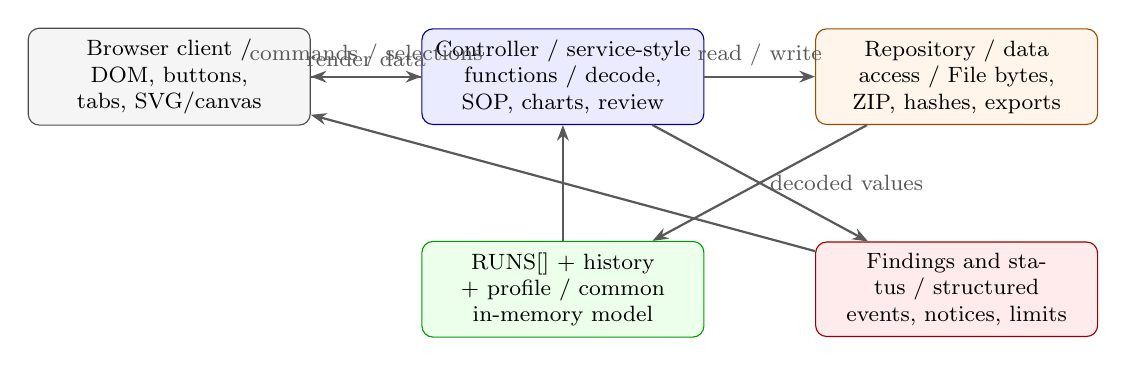
\begin{tikzpicture}[font=\footnotesize,box/.style={draw,rounded corners,align=center,minimum height=12mm,text width=3.3cm,inner sep=4pt,fill=#1!8,draw=#1!60!black},box/.default=blue,arr/.style={-{Stealth[length=2mm]},thick,gray!70!black}]
\node[box=gray] (client) at (0,0) {Browser client / DOM, buttons, tabs, SVG/canvas};
\node[box=blue] (svc) at (5,0) {Controller / service-style functions / decode, SOP, charts, review};
\node[box=orange] (repo) at (10,0) {Repository / data access / File bytes, ZIP, hashes, exports};
\node[box=green] (model) at (5,-2.7) {RUNS[] + history + profile / common in-memory model};
\node[box=red] (events) at (10,-2.7) {Findings and status / structured events, notices, limits};
\draw[arr] (client)--node[above]{commands / selections}(svc);
\draw[arr] (svc)--node[above]{read / write}(repo);
\draw[arr] (repo)--node[right]{decoded values}(model);
\draw[arr] (model)--(svc);
\draw[arr] (svc)--node[above]{render data}(client);
\draw[arr] (svc)--(events); \draw[arr] (events)--(client);
\end{tikzpicture}
\caption{Responsibility view of the current single-file page.}\label{fig:design-composition}
\end{figure}

\section{Intake and analysis activity}
\begin{figure}[htbp]\centering
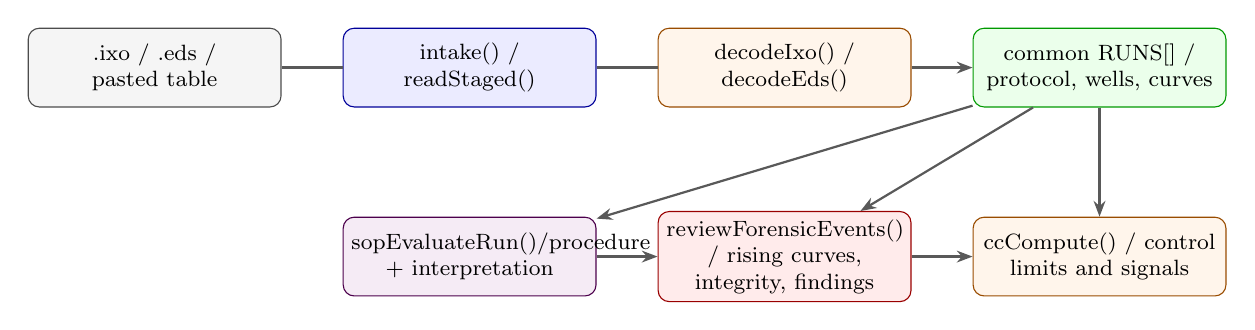
\begin{tikzpicture}[font=\footnotesize,box/.style={draw,rounded corners,align=center,minimum height=10mm,text width=3.0cm,inner sep=3pt,fill=#1!8,draw=#1!60!black},box/.default=blue,arr/.style={-{Stealth[length=2mm]},thick,gray!70!black}]
\node[box=gray](f) at (0,0){.ixo / .eds / pasted table};
\node[box=blue](i) at (4,0){intake() / readStaged()};
\node[box=orange](d) at (8,0){decodeIxo() / decodeEds()};
\node[box=green](m) at (12,0){common RUNS[] / protocol, wells, curves};
\node[box=violet](s) at (4,-2.4){sopEvaluateRun()/procedure + interpretation};
\node[box=red](q) at (8,-2.4){reviewForensicEvents() / rising curves, integrity, findings};
\node[box=orange](c) at (12,-2.4){ccCompute() / control limits and signals};
\draw[arr](f)--(i)--(d)--(m);\draw[arr](m)--(s);\draw[arr](m)--(q);\draw[arr](m)--(c); \draw[arr](s)--(q);\draw[arr](q)--(c);
\end{tikzpicture}
\caption{Activity view from staged files to method interpretation, forensic review and control charts.}\label{fig:design-activity}
\end{figure}

\section{Client-to-service sequence}
\begin{figure}[htbp]\centering
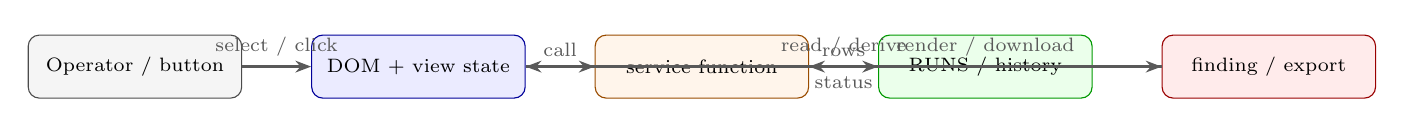
\begin{tikzpicture}[font=\scriptsize,box/.style={draw,rounded corners,align=center,minimum height=8mm,text width=2.5cm,inner sep=3pt,fill=#1!8,draw=#1!60!black},box/.default=blue,arr/.style={-{Stealth[length=2mm]},thick,gray!70!black}]
\node[box=gray](u) at (0,0){Operator / button};\node[box=blue](v) at (3.6,0){DOM + view state};\node[box=orange](x) at (7.2,0){service function};\node[box=green](r) at (10.8,0){RUNS / history};\node[box=red](e) at (14.4,0){finding / export};
\draw[arr](u)--node[above]{select / click}(v);\draw[arr](v)--node[above]{call}(x);\draw[arr](x)--node[above]{read / derive}(r);\draw[arr](r)--node[above]{rows}(x);\draw[arr](x)--node[above]{render / download}(e);\draw[arr](e)--node[below]{status}(v);
\end{tikzpicture}
\caption{Synchronous local sequence for a button action. No network or Java endpoint participates in the current implementation.}\label{fig:design-sequence}
\end{figure}

\section{Optional host integration boundary}
If a future Java host embeds the page, the boundary is an adapter around file selection and export delivery. The host may provide a file stream and receive a generated artifact, while the decoder, SOP engine, chart engine and evidence model remain deterministic page services. The contract should preserve the common run model and the profile hash; it must not rewrite stored Cq values or calls.

\section{Function-level flow records}
Table~\ref{tab:function-flow-map} is generated from the same current HTML snapshot as Appendix~\ref{app:index}; a changed function name or line range therefore appears in both places on the next build.
\begin{landscape}\scriptsize
\begin{longtable}{@{}p{3.2cm}p{1.45cm}p{2.7cm}p{4.0cm}p{4.0cm}p{3.0cm}@{}}
\caption{Function-level data-flow records for the current HTML snapshot.}\label{tab:function-flow-map}\\
\toprule Function & Lines & Responsibility & Inputs & Outputs & Next flow\\\midrule\endfirsthead
\toprule Function & Lines & Responsibility & Inputs & Outputs & Next flow\\\midrule\endhead
ZH\_TERMS & 996--1920 & Shared model / utility & primitive values or shared state & normalised value or configuration & utility → caller \\\hline
zhPhrase & 1924--2002 & Shared model / utility & primitive values or shared state & normalised value or configuration & utility → caller \\\hline
ui & 2003--2003 & Client / view & DOM state, selection, user command & HTML/SVG, status and download command & view state → render \\\hline
localizeDOM & 2004--2023 & Client / view & DOM state, selection, user command & HTML/SVG, status and download command & view state → render \\\hline
showCuteToast & 2024--2030 & Client / view & DOM state, selection, user command & HTML/SVG, status and download command & view state → render \\\hline
languageStorageKey & 2031--2031 & Client / view & DOM state, selection, user command & HTML/SVG, status and download command & view state → render \\\hline
rememberedLanguage & 2032--2032 & Client / view & DOM state, selection, user command & HTML/SVG, status and download command & view state → render \\\hline
setLanguage & 2033--2043 & Client / view & DOM state, selection, user command & HTML/SVG, status and download command & view state → render \\\hline
ROLES & 2045--2045 & Shared model / utility & primitive values or shared state & normalised value or configuration & utility → caller \\\hline
REP\_REGEX & 2046--2050 & Shared model / utility & primitive values or shared state & normalised value or configuration & utility → caller \\\hline
CALL & 2052--2052 & Shared model / utility & primitive values or shared state & normalised value or configuration & utility → caller \\\hline
SAMPLE\_TYPE & 2053--2057 & Shared model / utility & primitive values or shared state & normalised value or configuration & utility → caller \\\hline
TYPE\_TO\_ROLE & 2058--2062 & Shared model / utility & primitive values or shared state & normalised value or configuration & utility → caller \\\hline
NEGATIVE\_FAMILY & 2063--2063 & Shared model / utility & primitive values or shared state & normalised value or configuration & utility → caller \\\hline
ROLE\_COLOURS & 2064--2065 & Shared model / utility & primitive values or shared state & normalised value or configuration & utility → caller \\\hline
ROLE\_LINE & 2066--2067 & Shared model / utility & primitive values or shared state & normalised value or configuration & utility → caller \\\hline
PALETTE & 2068--2068 & Shared model / utility & primitive values or shared state & normalised value or configuration & utility → caller \\\hline
ce & 2070--2070 & Shared model / utility & primitive values or shared state & normalised value or configuration & utility → caller \\\hline
clone & 2077--2077 & Shared model / utility & primitive values or shared state & normalised value or configuration & utility → caller \\\hline
esc & 2078--2078 & Shared model / utility & primitive values or shared state & normalised value or configuration & utility → caller \\\hline
xesc & 2079--2079 & Shared model / utility & primitive values or shared state & normalised value or configuration & utility → caller \\\hline
safeName & 2080--2080 & Shared model / utility & primitive values or shared state & normalised value or configuration & utility → caller \\\hline
bytesFrom & 2081--2081 & Repository / data access & File bytes, decoded rows or export request & stored model, checksum or file bytes & repository → model/export \\\hline
scrollToEl & 2082--2082 & Client / view & DOM state, selection, user command & HTML/SVG, status and download command & view state → render \\\hline
option & 2083--2083 & Client / view & DOM state, selection, user command & HTML/SVG, status and download command & view state → render \\\hline
num & 2084--2084 & Shared model / utility & primitive values or shared state & normalised value or configuration & utility → caller \\\hline
safeRe & 2085--2085 & Shared model / utility & primitive values or shared state & normalised value or configuration & utility → caller \\\hline
uniq & 2086--2086 & Shared model / utility & primitive values or shared state & normalised value or configuration & utility → caller \\\hline
byKey & 2087--2087 & Shared model / utility & primitive values or shared state & normalised value or configuration & utility → caller \\\hline
mean & 2092--2092 & Shared model / utility & primitive values or shared state & normalised value or configuration & utility → caller \\\hline
sd & 2094--2094 & Shared model / utility & primitive values or shared state & normalised value or configuration & utility → caller \\\hline
median & 2095--2095 & Shared model / utility & primitive values or shared state & normalised value or configuration & utility → caller \\\hline
percentile & 2097--2102 & Shared model / utility & primitive values or shared state & normalised value or configuration & utility → caller \\\hline
range & 2103--2103 & Shared model / utility & primitive values or shared state & normalised value or configuration & utility → caller \\\hline
cv & 2104--2104 & Shared model / utility & primitive values or shared state & normalised value or configuration & utility → caller \\\hline
lgamma & 2107--2112 & Shared model / utility & primitive values or shared state & normalised value or configuration & utility → caller \\\hline
betacf & 2114--2133 & Shared model / utility & primitive values or shared state & normalised value or configuration & utility → caller \\\hline
betai & 2134--2138 & Shared model / utility & primitive values or shared state & normalised value or configuration & utility → caller \\\hline
tDistTwoTail & 2140--2143 & Shared model / utility & primitive values or shared state & normalised value or configuration & utility → caller \\\hline
gammap & 2145--2160 & Shared model / utility & primitive values or shared state & normalised value or configuration & utility → caller \\\hline
chiSqP & 2161--2161 & Shared model / utility & primitive values or shared state & normalised value or configuration & utility → caller \\\hline
tTest & 2164--2187 & Shared model / utility & primitive values or shared state & normalised value or configuration & utility → caller \\\hline
fitLin & 2188--2195 & Shared model / utility & primitive values or shared state & normalised value or configuration & utility → caller \\\hline
CRC\_TABLE & 2200--2200 & Client / view & DOM state, selection, user command & HTML/SVG, status and download command & view state → render \\\hline
crc32 & 2201--2201 & Repository / data access & File bytes, decoded rows or export request & stored model, checksum or file bytes & repository → model/export \\\hline
sourceSha256 & 2206--2212 & Repository / data access & File bytes, decoded rows or export request & stored model, checksum or file bytes & repository → model/export \\\hline
sha256Hex & 2213--2245 & Repository / data access & File bytes, decoded rows or export request & stored model, checksum or file bytes & repository → model/export \\\hline
inflate & 2246--2251 & Repository / data access & File bytes, decoded rows or export request & stored model, checksum or file bytes & repository → model/export \\\hline
readZip & 2253--2278 & Repository / data access & File bytes, decoded rows or export request & stored model, checksum or file bytes & repository → model/export \\\hline
dosStamp & 2279--2283 & Shared model / utility & primitive values or shared state & normalised value or configuration & utility → caller \\\hline
makeStoredZip & 2284--2309 & Repository / data access & File bytes, decoded rows or export request & stored model, checksum or file bytes & repository → model/export \\\hline
propText & 2317--2317 & Repository / data access & File bytes, decoded rows or export request & stored model, checksum or file bytes & repository → model/export \\\hline
pv & 2318--2318 & Shared model / utility & primitive values or shared state & normalised value or configuration & utility → caller \\\hline
propValues & 2319--2319 & Repository / data access & File bytes, decoded rows or export request & stored model, checksum or file bytes & repository → model/export \\\hline
base64ToBytes & 2320--2320 & Repository / data access & File bytes, decoded rows or export request & stored model, checksum or file bytes & repository → model/export \\\hline
posToWell & 2321--2321 & Shared model / utility & primitive values or shared state & normalised value or configuration & utility → caller \\\hline
posToLimsWell & 2322--2322 & Shared model / utility & primitive values or shared state & normalised value or configuration & utility → caller \\\hline
wellToPos & 2323--2326 & Shared model / utility & primitive values or shared state & normalised value or configuration & utility → caller \\\hline
hexBEToDouble & 2327--2334 & Shared model / utility & primitive values or shared state & normalised value or configuration & utility → caller \\\hline
decodeAcq & 2336--2423 & Controller / service & RUNS, profile, history or chart inputs & derived rows, findings, limits or calls & model → next service/view \\\hline
acquisitionStats & 2424--2431 & Client / view & DOM state, selection, user command & HTML/SVG, status and download command & view state → render \\\hline
decodePlateModel & 2434--2495 & Client / view & DOM state, selection, user command & HTML/SVG, status and download command & view state → render \\\hline
decodeSubsets & 2497--2507 & Controller / service & RUNS, profile, history or chart inputs & derived rows, findings, limits or calls & model → next service/view \\\hline
decodeProtocol & 2509--2544 & Controller / service & RUNS, profile, history or chart inputs & derived rows, findings, limits or calls & model → next service/view \\\hline
ANALYSIS\_KINDS & 2552--2560 & Controller / service & RUNS, profile, history or chart inputs & derived rows, findings, limits or calls & model → next service/view \\\hline
analysisKind & 2561--2565 & Controller / service & RUNS, profile, history or chart inputs & derived rows, findings, limits or calls & model → next service/view \\\hline
LC\_CALC\_STATE\_LABELS & 2570--2570 & Controller / service & RUNS, profile, history or chart inputs & derived rows, findings, limits or calls & model → next service/view \\\hline
calcStateLabel & 2571--2571 & Controller / service & RUNS, profile, history or chart inputs & derived rows, findings, limits or calls & model → next service/view \\\hline
cpMethodOf & 2572--2578 & Shared model / utility & primitive values or shared state & normalised value or configuration & utility → caller \\\hline
RESULT\_PROPS & 2580--2581 & Repository / data access & File bytes, decoded rows or export request & stored model, checksum or file bytes & repository → model/export \\\hline
readLists & 2582--2590 & Repository / data access & File bytes, decoded rows or export request & stored model, checksum or file bytes & repository → model/export \\\hline
resultKindOf & 2591--2601 & Shared model / utility & primitive values or shared state & normalised value or configuration & utility → caller \\\hline
PAIRING\_RULES & 2608--2608 & Shared model / utility & primitive values or shared state & normalised value or configuration & utility → caller \\\hline
rqResult & 2609--2625 & Shared model / utility & primitive values or shared state & normalised value or configuration & utility → caller \\\hline
decodeRelQuant & 2626--2672 & Controller / service & RUNS, profile, history or chart inputs & derived rows, findings, limits or calls & model → next service/view \\\hline
ownedBy & 2677--2685 & Shared model / utility & primitive values or shared state & normalised value or configuration & utility → caller \\\hline
ownQueryAll & 2686--2686 & Shared model / utility & primitive values or shared state & normalised value or configuration & utility → caller \\\hline
ownQuery & 2687--2687 & Shared model / utility & primitive values or shared state & normalised value or configuration & utility → caller \\\hline
decodeAnalyses & 2689--2776 & Controller / service & RUNS, profile, history or chart inputs & derived rows, findings, limits or calls & model → next service/view \\\hline
ownsResult & 2783--2791 & Shared model / utility & primitive values or shared state & normalised value or configuration & utility → caller \\\hline
analysisResults & 2792--2811 & Controller / service & RUNS, profile, history or chart inputs & derived rows, findings, limits or calls & model → next service/view \\\hline
decodeIxo & 2813--3155 & Controller / service & RUNS, profile, history or chart inputs & derived rows, findings, limits or calls & model → next service/view \\\hline
EDS & 3160--3708 & Shared model / utility & primitive values or shared state & normalised value or configuration & utility → caller \\\hline
\$ & 3163--3163 & Shared model / utility & primitive values or shared state & normalised value or configuration & utility → caller \\\hline
esc & 3164--3164 & Shared model / utility & primitive values or shared state & normalised value or configuration & utility → caller \\\hline
num & 3165--3165 & Shared model / utility & primitive values or shared state & normalised value or configuration & utility → caller \\\hline
fmt & 3166--3166 & Shared model / utility & primitive values or shared state & normalised value or configuration & utility → caller \\\hline
pill & 3167--3167 & Shared model / utility & primitive values or shared state & normalised value or configuration & utility → caller \\\hline
dt & 3168--3168 & Shared model / utility & primitive values or shared state & normalised value or configuration & utility → caller \\\hline
hex & 3169--3169 & Shared model / utility & primitive values or shared state & normalised value or configuration & utility → caller \\\hline
mean & 3170--3170 & Shared model / utility & primitive values or shared state & normalised value or configuration & utility → caller \\\hline
sd & 3171--3171 & Shared model / utility & primitive values or shared state & normalised value or configuration & utility → caller \\\hline
wellPos & 3173--3173 & Shared model / utility & primitive values or shared state & normalised value or configuration & utility → caller \\\hline
download & 3174--3178 & Repository / data access & File bytes, decoded rows or export request & stored model, checksum or file bytes & repository → model/export \\\hline
safeName & 3179--3179 & Shared model / utility & primitive values or shared state & normalised value or configuration & utility → caller \\\hline
CRC\_T & 3182--3182 & Repository / data access & File bytes, decoded rows or export request & stored model, checksum or file bytes & repository → model/export \\\hline
crc32 & 3183--3183 & Repository / data access & File bytes, decoded rows or export request & stored model, checksum or file bytes & repository → model/export \\\hline
MD5 & 3186--3213 & Shared model / utility & primitive values or shared state & normalised value or configuration & utility → caller \\\hline
inflateRaw & 3216--3221 & Repository / data access & File bytes, decoded rows or export request & stored model, checksum or file bytes & repository → model/export \\\hline
readZip & 3222--3249 & Repository / data access & File bytes, decoded rows or export request & stored model, checksum or file bytes & repository → model/export \\\hline
makeZip & 3252--3268 & Repository / data access & File bytes, decoded rows or export request & stored model, checksum or file bytes & repository → model/export \\\hline
xml & 3271--3271 & Shared model / utility & primitive values or shared state & normalised value or configuration & utility → caller \\\hline
kid & 3272--3272 & Shared model / utility & primitive values or shared state & normalised value or configuration & utility → caller \\\hline
kids & 3273--3273 & Shared model / utility & primitive values or shared state & normalised value or configuration & utility → caller \\\hline
txt & 3274--3274 & Shared model / utility & primitive values or shared state & normalised value or configuration & utility → caller \\\hline
argb & 3275--3275 & Shared model / utility & primitive values or shared state & normalised value or configuration & utility → caller \\\hline
bracketList & 3276--3276 & Shared model / utility & primitive values or shared state & normalised value or configuration & utility → caller \\\hline
ini & 3277--3279 & Shared model / utility & primitive values or shared state & normalised value or configuration & utility → caller \\\hline
FLAGS & 3284--3302 & Shared model / utility & primitive values or shared state & normalised value or configuration & utility → caller \\\hline
flagName & 3303--3303 & Shared model / utility & primitive values or shared state & normalised value or configuration & utility → caller \\\hline
parseEds & 3307--3513 & Controller / service & RUNS, profile, history or chart inputs & derived rows, findings, limits or calls & model → next service/view \\\hline
recalcCt & 3517--3521 & Controller / service & RUNS, profile, history or chart inputs & derived rows, findings, limits or calls & model → next service/view \\\hline
parseLog & 3523--3539 & Controller / service & RUNS, profile, history or chart inputs & derived rows, findings, limits or calls & model → next service/view \\\hline
studyRows & 3541--3545 & Shared model / utility & primitive values or shared state & normalised value or configuration & utility → caller \\\hline
QS\_DEFAULT\_COLS & 3553--3559 & Shared model / utility & primitive values or shared state & normalised value or configuration & utility → caller \\\hline
qsCols & 3560--3565 & Shared model / utility & primitive values or shared state & normalised value or configuration & utility → caller \\\hline
pad2 & 3566--3566 & Shared model / utility & primitive values or shared state & normalised value or configuration & utility → caller \\\hline
qsCalDate & 3567--3567 & Shared model / utility & primitive values or shared state & normalised value or configuration & utility → caller \\\hline
qsStamp & 3568--3572 & Shared model / utility & primitive values or shared state & normalised value or configuration & utility → caller \\\hline
qsRGB & 3573--3573 & Shared model / utility & primitive values or shared state & normalised value or configuration & utility → caller \\\hline
qsInstrument & 3576--3587 & Shared model / utility & primitive values or shared state & normalised value or configuration & utility → caller \\\hline
javaHashOrder & 3589--3593 & Shared model / utility & primitive values or shared state & normalised value or configuration & utility → caller \\\hline
qsHeader & 3594--3613 & Shared model / utility & primitive values or shared state & normalised value or configuration & utility → caller \\\hline
qsTables & 3614--3692 & Client / view & DOM state, selection, user command & HTML/SVG, status and download command & view state → render \\\hline
qsExport & 3693--3705 & Repository / data access & File bytes, decoded rows or export request & stored model, checksum or file bytes & repository → model/export \\\hline
QS\_DYE\_FILTER & 3721--3723 & Shared model / utility & primitive values or shared state & normalised value or configuration & utility → caller \\\hline
QS\_TASK\_ROLE & 3724--3725 & Shared model / utility & primitive values or shared state & normalised value or configuration & utility → caller \\\hline
QS\_AMP & 3726--3727 & Shared model / utility & primitive values or shared state & normalised value or configuration & utility → caller \\\hline
QS\_KIND & 3728--3729 & Shared model / utility & primitive values or shared state & normalised value or configuration & utility → caller \\\hline
isoLocal & 3730--3735 & Shared model / utility & primitive values or shared state & normalised value or configuration & utility → caller \\\hline
isEdsName & 3736--3736 & Shared model / utility & primitive values or shared state & normalised value or configuration & utility → caller \\\hline
decodeEds & 3737--3865 & Controller / service & RUNS, profile, history or chart inputs & derived rows, findings, limits or calls & model → next service/view \\\hline
ixoIntegrity & 3868--3882 & Repository / data access & File bytes, decoded rows or export request & stored model, checksum or file bytes & repository → model/export \\\hline
integrityLabel & 3883--3887 & Repository / data access & File bytes, decoded rows or export request & stored model, checksum or file bytes & repository → model/export \\\hline
integrityEvents & 3888--3903 & Controller / service & RUNS, profile, history or chart inputs & derived rows, findings, limits or calls & model → next service/view \\\hline
edsEvents & 3904--3987 & Controller / service & RUNS, profile, history or chart inputs & derived rows, findings, limits or calls & model → next service/view \\\hline
ec & 3988--3988 & Shared model / utility & primitive values or shared state & normalised value or configuration & utility → caller \\\hline
edsRecordTables & 3991--4036 & Client / view & DOM state, selection, user command & HTML/SVG, status and download command & view state → render \\\hline
drawTemperatureTrace & 4037--4049 & Client / view & DOM state, selection, user command & HTML/SVG, status and download command & view state → render \\\hline
edsDerived & 4052--4102 & Controller / service & RUNS, profile, history or chart inputs & derived rows, findings, limits or calls & model → next service/view \\\hline
pseudonymMap & 4106--4115 & Repository / data access & File bytes, decoded rows or export request & stored model, checksum or file bytes & repository → model/export \\\hline
pseudoOn & 4116--4116 & Shared model / utility & primitive values or shared state & normalised value or configuration & utility → caller \\\hline
exportName & 4117--4117 & Repository / data access & File bytes, decoded rows or export request & stored model, checksum or file bytes & repository → model/export \\\hline
pseudoRun & 4118--4125 & Controller / service & RUNS, profile, history or chart inputs & derived rows, findings, limits or calls & model → next service/view \\\hline
withExportNames & 4126--4130 & Repository / data access & File bytes, decoded rows or export request & stored model, checksum or file bytes & repository → model/export \\\hline
rqRows & 4131--4138 & Shared model / utility & primitive values or shared state & normalised value or configuration & utility → caller \\\hline
edsSignalRows & 4139--4155 & Shared model / utility & primitive values or shared state & normalised value or configuration & utility → caller \\\hline
xlsxCol & 4158--4158 & Repository / data access & File bytes, decoded rows or export request & stored model, checksum or file bytes & repository → model/export \\\hline
xlsxCell & 4159--4165 & Repository / data access & File bytes, decoded rows or export request & stored model, checksum or file bytes & repository → model/export \\\hline
makeXlsx & 4166--4180 & Repository / data access & File bytes, decoded rows or export request & stored model, checksum or file bytes & repository → model/export \\\hline
qsWorkbook & 4181--4188 & Shared model / utility & primitive values or shared state & normalised value or configuration & utility → caller \\\hline
reviewForensicEvents & 4190--4197 & Controller / service & RUNS, profile, history or chart inputs & derived rows, findings, limits or calls & model → next service/view \\\hline
SOP\_OUTCOMES & 4208--4208 & Controller / service & RUNS, profile, history or chart inputs & derived rows, findings, limits or calls & model → next service/view \\\hline
SOP\_OUTCOME\_DEFAULTS & 4209--4220 & Controller / service & RUNS, profile, history or chart inputs & derived rows, findings, limits or calls & model → next service/view \\\hline
sopBase & 4221--4237 & Controller / service & RUNS, profile, history or chart inputs & derived rows, findings, limits or calls & model → next service/view \\\hline
SOP\_PRESETS & 4238--4265 & Controller / service & RUNS, profile, history or chart inputs & derived rows, findings, limits or calls & model → next service/view \\\hline
STORED\_SOP & 4335--4335 & Controller / service & RUNS, profile, history or chart inputs & derived rows, findings, limits or calls & model → next service/view \\\hline
sopLoadStored & 4340--4340 & Controller / service & RUNS, profile, history or chart inputs & derived rows, findings, limits or calls & model → next service/view \\\hline
sopStore & 4341--4341 & Controller / service & RUNS, profile, history or chart inputs & derived rows, findings, limits or calls & model → next service/view \\\hline
sopMaybeSelectScDefault & 4342--4349 & Controller / service & RUNS, profile, history or chart inputs & derived rows, findings, limits or calls & model → next service/view \\\hline
sopNormalise & 4350--4364 & Controller / service & RUNS, profile, history or chart inputs & derived rows, findings, limits or calls & model → next service/view \\\hline
sopCanonical & 4365--4368 & Controller / service & RUNS, profile, history or chart inputs & derived rows, findings, limits or calls & model → next service/view \\\hline
sopHash & 4369--4369 & Controller / service & RUNS, profile, history or chart inputs & derived rows, findings, limits or calls & model → next service/view \\\hline
sopJSON & 4370--4370 & Controller / service & RUNS, profile, history or chart inputs & derived rows, findings, limits or calls & model → next service/view \\\hline
sopChanged & 4371--4371 & Controller / service & RUNS, profile, history or chart inputs & derived rows, findings, limits or calls & model → next service/view \\\hline
sopMatcher & 4374--4380 & Controller / service & RUNS, profile, history or chart inputs & derived rows, findings, limits or calls & model → next service/view \\\hline
sopNum & 4381--4381 & Controller / service & RUNS, profile, history or chart inputs & derived rows, findings, limits or calls & model → next service/view \\\hline
sopCq & 4382--4382 & Controller / service & RUNS, profile, history or chart inputs & derived rows, findings, limits or calls & model → next service/view \\\hline
sopOmitted & 4383--4383 & Controller / service & RUNS, profile, history or chart inputs & derived rows, findings, limits or calls & model → next service/view \\\hline
sopTargetSpec & 4384--4390 & Controller / service & RUNS, profile, history or chart inputs & derived rows, findings, limits or calls & model → next service/view \\\hline
sopRunApplicability & 4391--4401 & Controller / service & RUNS, profile, history or chart inputs & derived rows, findings, limits or calls & model → next service/view \\\hline
sopReplicateMinimum & 4402--4407 & Controller / service & RUNS, profile, history or chart inputs & derived rows, findings, limits or calls & model → next service/view \\\hline
CC\_TARGET\_ALIAS & 4410--4410 & Controller / service & RUNS, profile, history or chart inputs & derived rows, findings, limits or calls & model → next service/view \\\hline
ccCanonTarget & 4411--4411 & Controller / service & RUNS, profile, history or chart inputs & derived rows, findings, limits or calls & model → next service/view \\\hline
sopControlIdentity & 4412--4434 & Controller / service & RUNS, profile, history or chart inputs & derived rows, findings, limits or calls & model → next service/view \\\hline
sopLabScreening & 4435--4453 & Controller / service & RUNS, profile, history or chart inputs & derived rows, findings, limits or calls & model → next service/view \\\hline
ccBaselineNeed & 4454--4454 & Controller / service & RUNS, profile, history or chart inputs & derived rows, findings, limits or calls & model → next service/view \\\hline
ccNoDataReason & 4455--4460 & Controller / service & RUNS, profile, history or chart inputs & derived rows, findings, limits or calls & model → next service/view \\\hline
controlBatchRecords & 4461--4470 & Controller / service & RUNS, profile, history or chart inputs & derived rows, findings, limits or calls & model → next service/view \\\hline
controlBatchGraph & 4471--4487 & Client / view & DOM state, selection, user command & HTML/SVG, status and download command & view state → render \\\hline
sopControlSpec & 4489--4494 & Controller / service & RUNS, profile, history or chart inputs & derived rows, findings, limits or calls & model → next service/view \\\hline
sopFmt & 4495--4495 & Controller / service & RUNS, profile, history or chart inputs & derived rows, findings, limits or calls & model → next service/view \\\hline
sopTime & 4496--4500 & Controller / service & RUNS, profile, history or chart inputs & derived rows, findings, limits or calls & model → next service/view \\\hline
sopFmtTime & 4501--4502 & Controller / service & RUNS, profile, history or chart inputs & derived rows, findings, limits or calls & model → next service/view \\\hline
wellSignal & 4505--4510 & Shared model / utility & primitive values or shared state & normalised value or configuration & utility → caller \\\hline
runTimeline & 4513--4533 & Controller / service & RUNS, profile, history or chart inputs & derived rows, findings, limits or calls & model → next service/view \\\hline
runTimes & 4534--4541 & Controller / service & RUNS, profile, history or chart inputs & derived rows, findings, limits or calls & model → next service/view \\\hline
sopStdCurves & 4544--4557 & Controller / service & RUNS, profile, history or chart inputs & derived rows, findings, limits or calls & model → next service/view \\\hline
sopEvaluateRun & 4560--4696 & Controller / service & RUNS, profile, history or chart inputs & derived rows, findings, limits or calls & model → next service/view \\\hline
sopEvaluateAll & 4697--4701 & Controller / service & RUNS, profile, history or chart inputs & derived rows, findings, limits or calls & model → next service/view \\\hline
sopResultForWell & 4702--4705 & Controller / service & RUNS, profile, history or chart inputs & derived rows, findings, limits or calls & model → next service/view \\\hline
sopMeta & 4706--4706 & Controller / service & RUNS, profile, history or chart inputs & derived rows, findings, limits or calls & model → next service/view \\\hline
sopInterpretationRows & 4707--4718 & Controller / service & RUNS, profile, history or chart inputs & derived rows, findings, limits or calls & model → next service/view \\\hline
sopSampleRows & 4719--4732 & Controller / service & RUNS, profile, history or chart inputs & derived rows, findings, limits or calls & model → next service/view \\\hline
sopCriteriaRows & 4733--4736 & Controller / service & RUNS, profile, history or chart inputs & derived rows, findings, limits or calls & model → next service/view \\\hline
sopRunRows & 4737--4748 & Controller / service & RUNS, profile, history or chart inputs & derived rows, findings, limits or calls & model → next service/view \\\hline
sopEvents & 4749--4761 & Controller / service & RUNS, profile, history or chart inputs & derived rows, findings, limits or calls & model → next service/view \\\hline
invalidateAnalysisCaches & 4767--4769 & Controller / service & RUNS, profile, history or chart inputs & derived rows, findings, limits or calls & model → next service/view \\\hline
forensicSnapshot & 4770--4775 & Controller / service & RUNS, profile, history or chart inputs & derived rows, findings, limits or calls & model → next service/view \\\hline
extraForensicEvents & 4776--4776 & Controller / service & RUNS, profile, history or chart inputs & derived rows, findings, limits or calls & model → next service/view \\\hline
reviewForensicEventsCore & 4777--4777 & Controller / service & RUNS, profile, history or chart inputs & derived rows, findings, limits or calls & model → next service/view \\\hline
forensicCounts & 4778--4784 & Controller / service & RUNS, profile, history or chart inputs & derived rows, findings, limits or calls & model → next service/view \\\hline
extraForensicEventsUncached & 4785--4827 & Controller / service & RUNS, profile, history or chart inputs & derived rows, findings, limits or calls & model → next service/view \\\hline
sopOutcomeFor & 4832--4836 & Controller / service & RUNS, profile, history or chart inputs & derived rows, findings, limits or calls & model → next service/view \\\hline
SOP\_OUTCOME\_OPTIONS & 4837--4837 & Client / view & DOM state, selection, user command & HTML/SVG, status and download command & view state → render \\\hline
sopField & 4838--4847 & Controller / service & RUNS, profile, history or chart inputs & derived rows, findings, limits or calls & model → next service/view \\\hline
SOP\_ACTION\_LABEL & 4848--4850 & Controller / service & RUNS, profile, history or chart inputs & derived rows, findings, limits or calls & model → next service/view \\\hline
sopSetPath & 4851--4856 & Controller / service & RUNS, profile, history or chart inputs & derived rows, findings, limits or calls & model → next service/view \\\hline
sopTableEditor & 4857--4875 & Client / view & DOM state, selection, user command & HTML/SVG, status and download command & view state → render \\\hline
sopProfileEdited & 4876--4879 & Controller / service & RUNS, profile, history or chart inputs & derived rows, findings, limits or calls & model → next service/view \\\hline
renderSopHeader & 4880--4888 & Client / view & DOM state, selection, user command & HTML/SVG, status and download command & view state → render \\\hline
sopProcedureHTML & 4889--4908 & Controller / service & RUNS, profile, history or chart inputs & derived rows, findings, limits or calls & model → next service/view \\\hline
renderSopEditor & 4909--4999 & Client / view & DOM state, selection, user command & HTML/SVG, status and download command & view state → render \\\hline
SOP\_VIEW & 5000--5000 & Controller / service & RUNS, profile, history or chart inputs & derived rows, findings, limits or calls & model → next service/view \\\hline
renderSopResults & 5001--5048 & Client / view & DOM state, selection, user command & HTML/SVG, status and download command & view state → render \\\hline
sopCurrentRows & 5049--5052 & Client / view & DOM state, selection, user command & HTML/SVG, status and download command & view state → render \\\hline
csvOf & 5053--5053 & Repository / data access & File bytes, decoded rows or export request & stored model, checksum or file bytes & repository → model/export \\\hline
sheetOf & 5054--5054 & Shared model / utility & primitive values or shared state & normalised value or configuration & utility → caller \\\hline
sopReadme & 5055--5068 & Controller / service & RUNS, profile, history or chart inputs & derived rows, findings, limits or calls & model → next service/view \\\hline
sopDownloadWorkbook & 5069--5076 & Controller / service & RUNS, profile, history or chart inputs & derived rows, findings, limits or calls & model → next service/view \\\hline
sopDownloadBundle & 5077--5086 & Controller / service & RUNS, profile, history or chart inputs & derived rows, findings, limits or calls & model → next service/view \\\hline
wireSop & 5087--5103 & Client / view & DOM state, selection, user command & HTML/SVG, status and download command & view state → render \\\hline
renderSop & 5104--5104 & Client / view & DOM state, selection, user command & HTML/SVG, status and download command & view state → render \\\hline
renderResults & 5105--5105 & Client / view & DOM state, selection, user command & HTML/SVG, status and download command & view state → render \\\hline
svgEsc & 5108--5108 & Client / view & DOM state, selection, user command & HTML/SVG, status and download command & view state → render \\\hline
niceTicks & 5109--5116 & Shared model / utility & primitive values or shared state & normalised value or configuration & utility → caller \\\hline
fmtTick & 5117--5117 & Shared model / utility & primitive values or shared state & normalised value or configuration & utility → caller \\\hline
svgPlot & 5119--5163 & Client / view & DOM state, selection, user command & HTML/SVG, status and download command & view state → render \\\hline
svgMessage & 5164--5164 & Client / view & DOM state, selection, user command & HTML/SVG, status and download command & view state → render \\\hline
extent & 5165--5165 & Shared model / utility & primitive values or shared state & normalised value or configuration & utility → caller \\\hline
legendFromMap & 5166--5166 & Shared model / utility & primitive values or shared state & normalised value or configuration & utility → caller \\\hline
catColour & 5167--5167 & Shared model / utility & primitive values or shared state & normalised value or configuration & utility → caller \\\hline
sopColour & 5168--5168 & Controller / service & RUNS, profile, history or chart inputs & derived rows, findings, limits or calls & model → next service/view \\\hline
sopLabel & 5169--5169 & Controller / service & RUNS, profile, history or chart inputs & derived rows, findings, limits or calls & model → next service/view \\\hline
gRunWells & 5172--5172 & Controller / service & RUNS, profile, history or chart inputs & derived rows, findings, limits or calls & model → next service/view \\\hline
gTargets & 5173--5173 & Shared model / utility & primitive values or shared state & normalised value or configuration & utility → caller \\\hline
gCutLines & 5174--5180 & Shared model / utility & primitive values or shared state & normalised value or configuration & utility → caller \\\hline
gRunDate & 5183--5183 & Controller / service & RUNS, profile, history or chart inputs & derived rows, findings, limits or calls & model → next service/view \\\hline
gByDate & 5184--5184 & Shared model / utility & primitive values or shared state & normalised value or configuration & utility → caller \\\hline
gRunTicks & 5185--5190 & Controller / service & RUNS, profile, history or chart inputs & derived rows, findings, limits or calls & model → next service/view \\\hline
GRAPHS & 5191--5542 & Client / view & DOM state, selection, user command & HTML/SVG, status and download command & view state → render \\\hline
GRAPH\_METRICS & 5543--5543 & Client / view & DOM state, selection, user command & HTML/SVG, status and download command & view state → render \\\hline
GRAPH\_STATE & 5544--5544 & Client / view & DOM state, selection, user command & HTML/SVG, status and download command & view state → render \\\hline
graphContext & 5545--5550 & Client / view & DOM state, selection, user command & HTML/SVG, status and download command & view state → render \\\hline
renderGraphs & 5551--5580 & Client / view & DOM state, selection, user command & HTML/SVG, status and download command & view state → render \\\hline
graphFileBase & 5581--5581 & Client / view & DOM state, selection, user command & HTML/SVG, status and download command & view state → render \\\hline
graphSvgText & 5582--5583 & Client / view & DOM state, selection, user command & HTML/SVG, status and download command & view state → render \\\hline
graphPng & 5584--5591 & Client / view & DOM state, selection, user command & HTML/SVG, status and download command & view state → render \\\hline
graphAllZip & 5592--5612 & Client / view & DOM state, selection, user command & HTML/SVG, status and download command & view state → render \\\hline
wireGraphs & 5613--5625 & Client / view & DOM state, selection, user command & HTML/SVG, status and download command & view state → render \\\hline
markDirty & 5629--5629 & Shared model / utility & primitive values or shared state & normalised value or configuration & utility → caller \\\hline
currentTab & 5630--5630 & Client / view & DOM state, selection, user command & HTML/SVG, status and download command & view state → render \\\hline
currentReviewSheet & 5631--5631 & Client / view & DOM state, selection, user command & HTML/SVG, status and download command & view state → render \\\hline
REVIEW\_RENDERERS & 5632--5634 & Client / view & DOM state, selection, user command & HTML/SVG, status and download command & view state → render \\\hline
renderTab & 5635--5656 & Client / view & DOM state, selection, user command & HTML/SVG, status and download command & view state → render \\\hline
renderReviewSheetLazy & 5657--5661 & Client / view & DOM state, selection, user command & HTML/SVG, status and download command & view state → render \\\hline
ccLzss & 5676--5690 & Controller / service & RUNS, profile, history or chart inputs & derived rows, findings, limits or calls & model → next service/view \\\hline
ccDecodeArz & 5691--5704 & Controller / service & RUNS, profile, history or chart inputs & derived rows, findings, limits or calls & model → next service/view \\\hline
ccIxoTemperatureLog & 5705--5713 & Controller / service & RUNS, profile, history or chart inputs & derived rows, findings, limits or calls & model → next service/view \\\hline
ccIxoAcquisitions & 5716--5723 & Client / view & DOM state, selection, user command & HTML/SVG, status and download command & view state → render \\\hline
ccThermalSteps & 5726--5758 & Controller / service & RUNS, profile, history or chart inputs & derived rows, findings, limits or calls & model → next service/view \\\hline
ccTransitionPairs & 5766--5777 & Controller / service & RUNS, profile, history or chart inputs & derived rows, findings, limits or calls & model → next service/view \\\hline
ccTransitions & 5778--5804 & Controller / service & RUNS, profile, history or chart inputs & derived rows, findings, limits or calls & model → next service/view \\\hline
ccThin & 5807--5814 & Controller / service & RUNS, profile, history or chart inputs & derived rows, findings, limits or calls & model → next service/view \\\hline
ccPeakRates & 5815--5827 & Controller / service & RUNS, profile, history or chart inputs & derived rows, findings, limits or calls & model → next service/view \\\hline
ccThermalSummary & 5828--5836 & Controller / service & RUNS, profile, history or chart inputs & derived rows, findings, limits or calls & model → next service/view \\\hline
ccSetpoints & 5837--5840 & Controller / service & RUNS, profile, history or chart inputs & derived rows, findings, limits or calls & model → next service/view \\\hline
ccQsLog & 5843--5883 & Controller / service & RUNS, profile, history or chart inputs & derived rows, findings, limits or calls & model → next service/view \\\hline
ccCalibSummary & 5885--5895 & Controller / service & RUNS, profile, history or chart inputs & derived rows, findings, limits or calls & model → next service/view \\\hline
ccQuantSaturation & 5897--5902 & Controller / service & RUNS, profile, history or chart inputs & derived rows, findings, limits or calls & model → next service/view \\\hline
CC\_TZ & 5903--5903 & Controller / service & RUNS, profile, history or chart inputs & derived rows, findings, limits or calls & model → next service/view \\\hline
ccParseJavaDate & 5904--5908 & Controller / service & RUNS, profile, history or chart inputs & derived rows, findings, limits or calls & model → next service/view \\\hline
ccQ & 5911--5911 & Controller / service & RUNS, profile, history or chart inputs & derived rows, findings, limits or calls & model → next service/view \\\hline
ccMedian & 5912--5912 & Controller / service & RUNS, profile, history or chart inputs & derived rows, findings, limits or calls & model → next service/view \\\hline
ccStatic & 5913--5979 & Controller / service & RUNS, profile, history or chart inputs & derived rows, findings, limits or calls & model → next service/view \\\hline
ccDynamic & 5981--6030 & Controller / service & RUNS, profile, history or chart inputs & derived rows, findings, limits or calls & model → next service/view \\\hline
ccExtractOnLoad & 6032--6051 & Controller / service & RUNS, profile, history or chart inputs & derived rows, findings, limits or calls & model → next service/view \\\hline
ccProtocolKey & 6055--6058 & Controller / service & RUNS, profile, history or chart inputs & derived rows, findings, limits or calls & model → next service/view \\\hline
CC\_GROUPS & 6071--6075 & Controller / service & RUNS, profile, history or chart inputs & derived rows, findings, limits or calls & model → next service/view \\\hline
CC\_CHARTS & 6076--6260 & Controller / service & RUNS, profile, history or chart inputs & derived rows, findings, limits or calls & model → next service/view \\\hline
CC\_BY\_ID & 6261--6261 & Controller / service & RUNS, profile, history or chart inputs & derived rows, findings, limits or calls & model → next service/view \\\hline
CC\_DEFAULT\_CFG & 6262--6263 & Controller / service & RUNS, profile, history or chart inputs & derived rows, findings, limits or calls & model → next service/view \\\hline
ccCfg & 6267--6268 & Controller / service & RUNS, profile, history or chart inputs & derived rows, findings, limits or calls & model → next service/view \\\hline
ccSetCfg & 6269--6270 & Controller / service & RUNS, profile, history or chart inputs & derived rows, findings, limits or calls & model → next service/view \\\hline
CC\_C4 & 6273--6273 & Controller / service & RUNS, profile, history or chart inputs & derived rows, findings, limits or calls & model → next service/view \\\hline
ccPhase & 6274--6274 & Controller / service & RUNS, profile, history or chart inputs & derived rows, findings, limits or calls & model → next service/view \\\hline
ccI & 6276--6288 & Controller / service & RUNS, profile, history or chart inputs & derived rows, findings, limits or calls & model → next service/view \\\hline
ccWestgard & 6290--6300 & Controller / service & RUNS, profile, history or chart inputs & derived rows, findings, limits or calls & model → next service/view \\\hline
ccEWMA & 6301--6306 & Controller / service & RUNS, profile, history or chart inputs & derived rows, findings, limits or calls & model → next service/view \\\hline
ccCUSUM & 6307--6322 & Controller / service & RUNS, profile, history or chart inputs & derived rows, findings, limits or calls & model → next service/view \\\hline
ccTrend & 6324--6339 & Controller / service & RUNS, profile, history or chart inputs & derived rows, findings, limits or calls & model → next service/view \\\hline
ccP & 6340--6345 & Controller / service & RUNS, profile, history or chart inputs & derived rows, findings, limits or calls & model → next service/view \\\hline
ccU & 6346--6349 & Controller / service & RUNS, profile, history or chart inputs & derived rows, findings, limits or calls & model → next service/view \\\hline
ccC & 6350--6353 & Controller / service & RUNS, profile, history or chart inputs & derived rows, findings, limits or calls & model → next service/view \\\hline
ccXbarS & 6354--6365 & Controller / service & RUNS, profile, history or chart inputs & derived rows, findings, limits or calls & model → next service/view \\\hline
ccFunnel & 6366--6372 & Controller / service & RUNS, profile, history or chart inputs & derived rows, findings, limits or calls & model → next service/view \\\hline
CC\_LIMIT\_TEXT & 6375--6433 & Controller / service & RUNS, profile, history or chart inputs & derived rows, findings, limits or calls & model → next service/view \\\hline
CONSOLE\_DICT & 6434--6438 & Shared model / utility & primitive values or shared state & normalised value or configuration & utility → caller \\\hline
ccAlarmDir & 6439--6445 & Controller / service & RUNS, profile, history or chart inputs & derived rows, findings, limits or calls & model → next service/view \\\hline
CC\_STATE & 6450--6450 & Controller / service & RUNS, profile, history or chart inputs & derived rows, findings, limits or calls & model → next service/view \\\hline
CC\_COL & 6452--6452 & Controller / service & RUNS, profile, history or chart inputs & derived rows, findings, limits or calls & model → next service/view \\\hline
CC\_SEG\_PALETTE & 6456--6456 & Controller / service & RUNS, profile, history or chart inputs & derived rows, findings, limits or calls & model → next service/view \\\hline
ccSignal & 6458--6458 & Controller / service & RUNS, profile, history or chart inputs & derived rows, findings, limits or calls & model → next service/view \\\hline
ccPlatform & 6459--6459 & Controller / service & RUNS, profile, history or chart inputs & derived rows, findings, limits or calls & model → next service/view \\\hline
ccInstrumentKey & 6460--6460 & Controller / service & RUNS, profile, history or chart inputs & derived rows, findings, limits or calls & model → next service/view \\\hline
ccOperator & 6461--6461 & Controller / service & RUNS, profile, history or chart inputs & derived rows, findings, limits or calls & model → next service/view \\\hline
ccRowsFromRuns & 6463--6477 & Controller / service & RUNS, profile, history or chart inputs & derived rows, findings, limits or calls & model → next service/view \\\hline
ccAllRows & 6478--6481 & Controller / service & RUNS, profile, history or chart inputs & derived rows, findings, limits or calls & model → next service/view \\\hline
ccInstruments & 6482--6482 & Controller / service & RUNS, profile, history or chart inputs & derived rows, findings, limits or calls & model → next service/view \\\hline
ccRowsFor & 6483--6488 & Controller / service & RUNS, profile, history or chart inputs & derived rows, findings, limits or calls & model → next service/view \\\hline
ccVariants & 6490--6492 & Controller / service & RUNS, profile, history or chart inputs & derived rows, findings, limits or calls & model → next service/view \\\hline
ccValue & 6493--6495 & Controller / service & RUNS, profile, history or chart inputs & derived rows, findings, limits or calls & model → next service/view \\\hline
ccXAxis & 6496--6502 & Controller / service & RUNS, profile, history or chart inputs & derived rows, findings, limits or calls & model → next service/view \\\hline
ccSpec & 6503--6508 & Controller / service & RUNS, profile, history or chart inputs & derived rows, findings, limits or calls & model → next service/view \\\hline
ccCompute & 6509--6559 & Controller / service & RUNS, profile, history or chart inputs & derived rows, findings, limits or calls & model → next service/view \\\hline
ccShift & 6563--6574 & Controller / service & RUNS, profile, history or chart inputs & derived rows, findings, limits or calls & model → next service/view \\\hline
ccStatus & 6575--6600 & Controller / service & RUNS, profile, history or chart inputs & derived rows, findings, limits or calls & model → next service/view \\\hline
ccSpark & 6602--6612 & Controller / service & RUNS, profile, history or chart inputs & derived rows, findings, limits or calls & model → next service/view \\\hline
ccVersionMarks & 6613--6617 & Controller / service & RUNS, profile, history or chart inputs & derived rows, findings, limits or calls & model → next service/view \\\hline
ccChartSvg & 6618--6677 & Client / view & DOM state, selection, user command & HTML/SVG, status and download command & view state → render \\\hline
ccSChartSvg & 6678--6684 & Client / view & DOM state, selection, user command & HTML/SVG, status and download command & view state → render \\\hline
renderPanel & 6686--6726 & Client / view & DOM state, selection, user command & HTML/SVG, status and download command & view state → render \\\hline
renderCcDetail & 6727--6796 & Client / view & DOM state, selection, user command & HTML/SVG, status and download command & view state → render \\\hline
ccPng & 6797--6802 & Controller / service & RUNS, profile, history or chart inputs & derived rows, findings, limits or calls & model → next service/view \\\hline
ccChartRows & 6803--6810 & Controller / service & RUNS, profile, history or chart inputs & derived rows, findings, limits or calls & model → next service/view \\\hline
ccSvgToPng & 6811--6816 & Client / view & DOM state, selection, user command & HTML/SVG, status and download command & view state → render \\\hline
ccZipAll & 6820--6868 & Controller / service & RUNS, profile, history or chart inputs & derived rows, findings, limits or calls & model → next service/view \\\hline
ccHistoryJSON & 6870--6874 & Controller / service & RUNS, profile, history or chart inputs & derived rows, findings, limits or calls & model → next service/view \\\hline
ccHistoryCSV & 6875--6881 & Controller / service & RUNS, profile, history or chart inputs & derived rows, findings, limits or calls & model → next service/view \\\hline
ccMigrateControlKeys & 6883--6895 & Controller / service & RUNS, profile, history or chart inputs & derived rows, findings, limits or calls & model → next service/view \\\hline
ccImport & 6896--6904 & Controller / service & RUNS, profile, history or chart inputs & derived rows, findings, limits or calls & model → next service/view \\\hline
ccRemember & 6905--6905 & Controller / service & RUNS, profile, history or chart inputs & derived rows, findings, limits or calls & model → next service/view \\\hline
ccRestore & 6906--6906 & Controller / service & RUNS, profile, history or chart inputs & derived rows, findings, limits or calls & model → next service/view \\\hline
ccEvents & 6908--6919 & Controller / service & RUNS, profile, history or chart inputs & derived rows, findings, limits or calls & model → next service/view \\\hline
wirePanel & 6921--6938 & Client / view & DOM state, selection, user command & HTML/SVG, status and download command & view state → render \\\hline
effWol & 6952--6970 & Shared model / utility & primitive values or shared state & normalised value or configuration & utility → caller \\\hline
effSliwinProxy & 6971--6984 & Shared model / utility & primitive values or shared state & normalised value or configuration & utility → caller \\\hline
efficiencyFromSlope & 6991--6995 & Shared model / utility & primitive values or shared state & normalised value or configuration & utility → caller \\\hline
\$ & 7000--7000 & Shared model / utility & primitive values or shared state & normalised value or configuration & utility → caller \\\hline
\$\$ & 7001--7001 & Shared model / utility & primitive values or shared state & normalised value or configuration & utility → caller \\\hline
APP\_LIMITS & 7006--7006 & Shared model / utility & primitive values or shared state & normalised value or configuration & utility → caller \\\hline
APP\_STATE & 7007--7007 & Controller / service & RUNS, profile, history or chart inputs & derived rows, findings, limits or calls & model → next service/view \\\hline
appError & 7008--7015 & Shared model / utility & primitive values or shared state & normalised value or configuration & utility → caller \\\hline
APP\_PHASE\_TRANSITIONS & 7016--7016 & Shared model / utility & primitive values or shared state & normalised value or configuration & utility → caller \\\hline
setPhase & 7017--7026 & Shared model / utility & primitive values or shared state & normalised value or configuration & utility → caller \\\hline
appDiagnostics & 7027--7027 & Shared model / utility & primitive values or shared state & normalised value or configuration & utility → caller \\\hline
validateRunBoundary & 7028--7037 & Controller / service & RUNS, profile, history or chart inputs & derived rows, findings, limits or calls & model → next service/view \\\hline
validateHistoryBoundary & 7038--7045 & Shared model / utility & primitive values or shared state & normalised value or configuration & utility → caller \\\hline
MG & 7055--7055 & Client / view & DOM state, selection, user command & HTML/SVG, status and download command & view state → render \\\hline
MG\_GLYPH & 7056--7056 & Client / view & DOM state, selection, user command & HTML/SVG, status and download command & view state → render \\\hline
MG\_WORD & 7057--7057 & Client / view & DOM state, selection, user command & HTML/SVG, status and download command & view state → render \\\hline
mgBuildQueue & 7060--7177 & Client / view & DOM state, selection, user command & HTML/SVG, status and download command & view state → render \\\hline
mgItem & 7180--7180 & Client / view & DOM state, selection, user command & HTML/SVG, status and download command & view state → render \\\hline
MG\_TYPE\_LABEL & 7181--7181 & Client / view & DOM state, selection, user command & HTML/SVG, status and download command & view state → render \\\hline
mgChartTypeOptions & 7182--7186 & Client / view & DOM state, selection, user command & HTML/SVG, status and download command & view state → render \\\hline
mgChartAxisOptions & 7187--7194 & Client / view & DOM state, selection, user command & HTML/SVG, status and download command & view state → render \\\hline
mgStatusPaint & 7195--7204 & Client / view & DOM state, selection, user command & HTML/SVG, status and download command & view state → render \\\hline
mgRender & 7206--7284 & Client / view & DOM state, selection, user command & HTML/SVG, status and download command & view state → render \\\hline
mgSheet & 7287--7301 & Client / view & DOM state, selection, user command & HTML/SVG, status and download command & view state → render \\\hline
mgSheetPick & 7302--7307 & Client / view & DOM state, selection, user command & HTML/SVG, status and download command & view state → render \\\hline
mgSheetClose & 7308--7308 & Client / view & DOM state, selection, user command & HTML/SVG, status and download command & view state → render \\\hline
mgItemSentence & 7309--7313 & Client / view & DOM state, selection, user command & HTML/SVG, status and download command & view state → render \\\hline
mgStage & 7321--7326 & Client / view & DOM state, selection, user command & HTML/SVG, status and download command & view state → render \\\hline
mgStageSet & 7327--7327 & Client / view & DOM state, selection, user command & HTML/SVG, status and download command & view state → render \\\hline
mgApplyChartView & 7328--7335 & Client / view & DOM state, selection, user command & HTML/SVG, status and download command & view state → render \\\hline
mgZoom & 7336--7342 & Client / view & DOM state, selection, user command & HTML/SVG, status and download command & view state → render \\\hline
mgPan & 7343--7343 & Client / view & DOM state, selection, user command & HTML/SVG, status and download command & view state → render \\\hline
MG\_COMMANDS & 7345--7376 & Client / view & DOM state, selection, user command & HTML/SVG, status and download command & view state → render \\\hline
mgCommand & 7377--7394 & Client / view & DOM state, selection, user command & HTML/SVG, status and download command & view state → render \\\hline
mgGo & 7395--7400 & Client / view & DOM state, selection, user command & HTML/SVG, status and download command & view state → render \\\hline
mgGoChart & 7401--7409 & Client / view & DOM state, selection, user command & HTML/SVG, status and download command & view state → render \\\hline
mgSetChartType & 7410--7413 & Client / view & DOM state, selection, user command & HTML/SVG, status and download command & view state → render \\\hline
mgSetChartAxis & 7414--7417 & Client / view & DOM state, selection, user command & HTML/SVG, status and download command & view state → render \\\hline
mgReadFiles & 7418--7424 & Client / view & DOM state, selection, user command & HTML/SVG, status and download command & view state → render \\\hline
mgChooseFiles & 7425--7429 & Client / view & DOM state, selection, user command & HTML/SVG, status and download command & view state → render \\\hline
mgLeaveTo & 7430--7430 & Client / view & DOM state, selection, user command & HTML/SVG, status and download command & view state → render \\\hline
MG\_PICT & 7443--7444 & Client / view & DOM state, selection, user command & HTML/SVG, status and download command & view state → render \\\hline
mgIt & 7445--7446 & Client / view & DOM state, selection, user command & HTML/SVG, status and download command & view state → render \\\hline
mgSafe & 7447--7447 & Client / view & DOM state, selection, user command & HTML/SVG, status and download command & view state → render \\\hline
mgTxt & 7448--7448 & Client / view & DOM state, selection, user command & HTML/SVG, status and download command & view state → render \\\hline
mgViewLoad & 7451--7506 & Client / view & DOM state, selection, user command & HTML/SVG, status and download command & view state → render \\\hline
mgViewSop & 7509--7575 & Client / view & DOM state, selection, user command & HTML/SVG, status and download command & view state → render \\\hline
mgViewResults & 7578--7656 & Client / view & DOM state, selection, user command & HTML/SVG, status and download command & view state → render \\\hline
mgPanelItems & 7659--7696 & Client / view & DOM state, selection, user command & HTML/SVG, status and download command & view state → render \\\hline
mgViewPanel & 7697--7719 & Client / view & DOM state, selection, user command & HTML/SVG, status and download command & view state → render \\\hline
mgGraphCtx & 7722--7726 & Client / view & DOM state, selection, user command & HTML/SVG, status and download command & view state → render \\\hline
mgViewGraphs & 7727--7755 & Client / view & DOM state, selection, user command & HTML/SVG, status and download command & view state → render \\\hline
mgViewReview & 7758--7788 & Client / view & DOM state, selection, user command & HTML/SVG, status and download command & view state → render \\\hline
mgViewIntegrity & 7791--7803 & Client / view & DOM state, selection, user command & HTML/SVG, status and download command & view state → render \\\hline
mgViewExport & 7806--7831 & Client / view & DOM state, selection, user command & HTML/SVG, status and download command & view state → render \\\hline
MG\_VIEWS & 7833--7842 & Client / view & DOM state, selection, user command & HTML/SVG, status and download command & view state → render \\\hline
mgScope & 7843--7846 & Client / view & DOM state, selection, user command & HTML/SVG, status and download command & view state → render \\\hline
mgScopeMark & 7847--7850 & Client / view & DOM state, selection, user command & HTML/SVG, status and download command & view state → render \\\hline
mgItemKey & 7851--7851 & Client / view & DOM state, selection, user command & HTML/SVG, status and download command & view state → render \\\hline
mgScopeFilter & 7854--7859 & Client / view & DOM state, selection, user command & HTML/SVG, status and download command & view state → render \\\hline
mgRefresh & 7860--7874 & Client / view & DOM state, selection, user command & HTML/SVG, status and download command & view state → render \\\hline
mgOpen & 7878--7882 & Client / view & DOM state, selection, user command & HTML/SVG, status and download command & view state → render \\\hline
mgClose & 7883--7885 & Client / view & DOM state, selection, user command & HTML/SVG, status and download command & view state → render \\\hline
mgToggle & 7886--7886 & Client / view & DOM state, selection, user command & HTML/SVG, status and download command & view state → render \\\hline
mgInit & 7887--7897 & Client / view & DOM state, selection, user command & HTML/SVG, status and download command & view state → render \\\hline
APP\_STATS & 7904--7904 & Shared model / utility & primitive values or shared state & normalised value or configuration & utility → caller \\\hline
appTaskStart & 7905--7909 & Shared model / utility & primitive values or shared state & normalised value or configuration & utility → caller \\\hline
appTaskStep & 7910--7910 & Shared model / utility & primitive values or shared state & normalised value or configuration & utility → caller \\\hline
appTaskEnd & 7911--7915 & Shared model / utility & primitive values or shared state & normalised value or configuration & utility → caller \\\hline
appTaskWrap & 7916--7919 & Shared model / utility & primitive values or shared state & normalised value or configuration & utility → caller \\\hline
APP\_TASK\_LABEL & 7920--7922 & Shared model / utility & primitive values or shared state & normalised value or configuration & utility → caller \\\hline
appHeapMB & 7923--7923 & Shared model / utility & primitive values or shared state & normalised value or configuration & utility → caller \\\hline
appStagedBytes & 7924--7924 & Repository / data access & File bytes, decoded rows or export request & stored model, checksum or file bytes & repository → model/export \\\hline
appNotice & 7925--7930 & Shared model / utility & primitive values or shared state & normalised value or configuration & utility → caller \\\hline
appCancel & 7931--7935 & Shared model / utility & primitive values or shared state & normalised value or configuration & utility → caller \\\hline
appReadSuperseded & 7936--7943 & Repository / data access & File bytes, decoded rows or export request & stored model, checksum or file bytes & repository → model/export \\\hline
APP\_PHASE\_TEXT & 7944--7945 & Shared model / utility & primitive values or shared state & normalised value or configuration & utility → caller \\\hline
appFmtMs & 7946--7946 & Shared model / utility & primitive values or shared state & normalised value or configuration & utility → caller \\\hline
appFmtMB & 7947--7947 & Shared model / utility & primitive values or shared state & normalised value or configuration & utility → caller \\\hline
appStatusSnapshot & 7948--7961 & Shared model / utility & primitive values or shared state & normalised value or configuration & utility → caller \\\hline
renderConsoleIdentity & 7962--7973 & Client / view & DOM state, selection, user command & HTML/SVG, status and download command & view state → render \\\hline
appStatusPaint & 7975--8022 & Shared model / utility & primitive values or shared state & normalised value or configuration & utility → caller \\\hline
appStatusReport & 8023--8028 & Shared model / utility & primitive values or shared state & normalised value or configuration & utility → caller \\\hline
appStatusInit & 8029--8040 & Shared model / utility & primitive values or shared state & normalised value or configuration & utility → caller \\\hline
RUNS & 8041--8041 & Controller / service & RUNS, profile, history or chart inputs & derived rows, findings, limits or calls & model → next service/view \\\hline
tag & 8045--8045 & Shared model / utility & primitive values or shared state & normalised value or configuration & utility → caller \\\hline
table & 8046--8054 & Client / view & DOM state, selection, user command & HTML/SVG, status and download command & view state → render \\\hline
download & 8055--8061 & Repository / data access & File bytes, decoded rows or export request & stored model, checksum or file bytes & repository → model/export \\\hline
websiteSource & 8062--8065 & Repository / data access & File bytes, decoded rows or export request & stored model, checksum or file bytes & repository → model/export \\\hline
makeWebsiteArchive & 8066--8072 & Shared model / utility & primitive values or shared state & normalised value or configuration & utility → caller \\\hline
downloadWebsiteArchive & 8073--8076 & Repository / data access & File bytes, decoded rows or export request & stored model, checksum or file bytes & repository → model/export \\\hline
csvq & 8077--8080 & Repository / data access & File bytes, decoded rows or export request & stored model, checksum or file bytes & repository → model/export \\\hline
toCSV & 8081--8084 & Repository / data access & File bytes, decoded rows or export request & stored model, checksum or file bytes & repository → model/export \\\hline
stamp & 8085--8085 & Shared model / utility & primitive values or shared state & normalised value or configuration & utility → caller \\\hline
baseName & 8086--8090 & Shared model / utility & primitive values or shared state & normalised value or configuration & utility → caller \\\hline
NAME\_ROLE\_RULES & 8103--8110 & Shared model / utility & primitive values or shared state & normalised value or configuration & utility → caller \\\hline
roleFromName & 8111--8115 & Shared model / utility & primitive values or shared state & normalised value or configuration & utility → caller \\\hline
assignRoles & 8116--8143 & Shared model / utility & primitive values or shared state & normalised value or configuration & utility → caller \\\hline
operatorOf & 8148--8148 & Shared model / utility & primitive values or shared state & normalised value or configuration & utility → caller \\\hline
sourceUidOf & 8149--8149 & Client / view & DOM state, selection, user command & HTML/SVG, status and download command & view state → render \\\hline
sourceCRCOf & 8150--8150 & Repository / data access & File bytes, decoded rows or export request & stored model, checksum or file bytes & repository → model/export \\\hline
sourceSHA256Of & 8151--8151 & Repository / data access & File bytes, decoded rows or export request & stored model, checksum or file bytes & repository → model/export \\\hline
runDurationMinutes & 8152--8155 & Controller / service & RUNS, profile, history or chart inputs & derived rows, findings, limits or calls & model → next service/view \\\hline
uniqueCurveCount & 8156--8158 & Controller / service & RUNS, profile, history or chart inputs & derived rows, findings, limits or calls & model → next service/view \\\hline
acquiredCurveCount & 8159--8159 & Client / view & DOM state, selection, user command & HTML/SVG, status and download command & view state → render \\\hline
wellRows & 8160--8190 & Shared model / utility & primitive values or shared state & normalised value or configuration & utility → caller \\\hline
allWellRows & 8191--8191 & Shared model / utility & primitive values or shared state & normalised value or configuration & utility → caller \\\hline
tmRows & 8192--8214 & Shared model / utility & primitive values or shared state & normalised value or configuration & utility → caller \\\hline
metaRows & 8215--8238 & Shared model / utility & primitive values or shared state & normalised value or configuration & utility → caller \\\hline
dyeChemistryOf & 8254--8263 & Shared model / utility & primitive values or shared state & normalised value or configuration & utility → caller \\\hline
rdmlSampleType & 8264--8269 & Repository / data access & File bytes, decoded rows or export request & stored model, checksum or file bytes & repository → model/export \\\hline
rdmlId & 8270--8270 & Repository / data access & File bytes, decoded rows or export request & stored model, checksum or file bytes & repository → model/export \\\hline
analysisGroups & 8271--8279 & Controller / service & RUNS, profile, history or chart inputs & derived rows, findings, limits or calls & model → next service/view \\\hline
curveAnalysisGroups & 8280--8280 & Controller / service & RUNS, profile, history or chart inputs & derived rows, findings, limits or calls & model → next service/view \\\hline
makeRDMLXML & 8282--8325 & Repository / data access & File bytes, decoded rows or export request & stored model, checksum or file bytes & repository → model/export \\\hline
makeRDML & 8326--8326 & Repository / data access & File bytes, decoded rows or export request & stored model, checksum or file bytes & repository → model/export \\\hline
makeQpcrWide & 8331--8343 & Shared model / utility & primitive values or shared state & normalised value or configuration & utility → caller \\\hline
makeQpcrWideTables & 8344--8351 & Client / view & DOM state, selection, user command & HTML/SVG, status and download command & view state → render \\\hline
makeBaselineCSV & 8355--8367 & Repository / data access & File bytes, decoded rows or export request & stored model, checksum or file bytes & repository → model/export \\\hline
makeRDES & 8368--8380 & Repository / data access & File bytes, decoded rows or export request & stored model, checksum or file bytes & repository → model/export \\\hline
makeRDESTables & 8381--8388 & Client / view & DOM state, selection, user command & HTML/SVG, status and download command & view state → render \\\hline
rScript & 8391--8429 & Shared model / utility & primitive values or shared state & normalised value or configuration & utility → caller \\\hline
pyScript & 8430--8468 & Shared model / utility & primitive values or shared state & normalised value or configuration & utility → caller \\\hline
BASE\_MACHINE\_METADATA & 8473--8473 & Repository / data access & File bytes, decoded rows or export request & stored model, checksum or file bytes & repository → model/export \\\hline
JSONLD\_STANDARDS & 8474--8480 & Shared model / utility & primitive values or shared state & normalised value or configuration & utility → caller \\\hline
metadataId & 8481--8484 & Repository / data access & File bytes, decoded rows or export request & stored model, checksum or file bytes & repository → model/export \\\hline
outputDistribution & 8485--8491 & Shared model / utility & primitive values or shared state & normalised value or configuration & utility → caller \\\hline
distributionsFor & 8492--8519 & Shared model / utility & primitive values or shared state & normalised value or configuration & utility → caller \\\hline
variablesFor & 8520--8527 & Shared model / utility & primitive values or shared state & normalised value or configuration & utility → caller \\\hline
datasetMetadata & 8528--8573 & Repository / data access & File bytes, decoded rows or export request & stored model, checksum or file bytes & repository → model/export \\\hline
pastedDatasetMetadata & 8574--8585 & Repository / data access & File bytes, decoded rows or export request & stored model, checksum or file bytes & repository → model/export \\\hline
machineMetadataDocument & 8586--8598 & Repository / data access & File bytes, decoded rows or export request & stored model, checksum or file bytes & repository → model/export \\\hline
machineMetadataJSON & 8599--8599 & Repository / data access & File bytes, decoded rows or export request & stored model, checksum or file bytes & repository → model/export \\\hline
renderMachineMetadata & 8600--8603 & Client / view & DOM state, selection, user command & HTML/SVG, status and download command & view state → render \\\hline
exportCatalogue & 8604--8640 & Repository / data access & File bytes, decoded rows or export request & stored model, checksum or file bytes & repository → model/export \\\hline
exportCatalogueCore & 8641--8693 & Repository / data access & File bytes, decoded rows or export request & stored model, checksum or file bytes & repository → model/export \\\hline
bundleZip & 8694--8737 & Repository / data access & File bytes, decoded rows or export request & stored model, checksum or file bytes & repository → model/export \\\hline
bundleReadme & 8738--8780 & Repository / data access & File bytes, decoded rows or export request & stored model, checksum or file bytes & repository → model/export \\\hline
renderLoaded & 8786--8816 & Client / view & DOM state, selection, user command & HTML/SVG, status and download command & view state → render \\\hline
renderDiagnostics & 8817--8833 & Client / view & DOM state, selection, user command & HTML/SVG, status and download command & view state → render \\\hline
renderExports & 8834--8873 & Client / view & DOM state, selection, user command & HTML/SVG, status and download command & view state → render \\\hline
REVIEW\_COLOURS & 8882--8888 & Controller / service & RUNS, profile, history or chart inputs & derived rows, findings, limits or calls & model → next service/view \\\hline
PLATE\_PASTELS & 8889--8889 & Shared model / utility & primitive values or shared state & normalised value or configuration & utility → caller \\\hline
CONTROL\_CATEGORY\_OPTIONS & 8890--8892 & Client / view & DOM state, selection, user command & HTML/SVG, status and download command & view state → render \\\hline
REVIEW\_STATE & 8893--8894 & Controller / service & RUNS, profile, history or chart inputs & derived rows, findings, limits or calls & model → next service/view \\\hline
runName & 8896--8896 & Controller / service & RUNS, profile, history or chart inputs & derived rows, findings, limits or calls & model → next service/view \\\hline
shortDate & 8897--8900 & Shared model / utility & primitive values or shared state & normalised value or configuration & utility → caller \\\hline
displayRunTick & 8901--8904 & Controller / service & RUNS, profile, history or chart inputs & derived rows, findings, limits or calls & model → next service/view \\\hline
runAt & 8905--8908 & Controller / service & RUNS, profile, history or chart inputs & derived rows, findings, limits or calls & model → next service/view \\\hline
setSelectItems & 8909--8916 & Client / view & DOM state, selection, user command & HTML/SVG, status and download command & view state → render \\\hline
analysisChoices & 8918--8928 & Controller / service & RUNS, profile, history or chart inputs & derived rows, findings, limits or calls & model → next service/view \\\hline
selectedWells & 8929--8933 & Shared model / utility & primitive values or shared state & normalised value or configuration & utility → caller \\\hline
physicalCurveRows & 8934--8950 & Controller / service & RUNS, profile, history or chart inputs & derived rows, findings, limits or calls & model → next service/view \\\hline
heatColour & 8951--8956 & Client / view & DOM state, selection, user command & HTML/SVG, status and download command & view state → render \\\hline
plateMapRows & 8957--8984 & Shared model / utility & primitive values or shared state & normalised value or configuration & utility → caller \\\hline
sampleComparisonRows & 8985--8998 & Shared model / utility & primitive values or shared state & normalised value or configuration & utility → caller \\\hline
reviewStatisticsRows & 8999--9018 & Controller / service & RUNS, profile, history or chart inputs & derived rows, findings, limits or calls & model → next service/view \\\hline
replicateReviewRows & 9019--9033 & Controller / service & RUNS, profile, history or chart inputs & derived rows, findings, limits or calls & model → next service/view \\\hline
BLANK\_ROLES & 9040--9040 & Shared model / utility & primitive values or shared state & normalised value or configuration & utility → caller \\\hline
orphanBlankRole & 9041--9047 & Controller / service & RUNS, profile, history or chart inputs & derived rows, findings, limits or calls & model → next service/view \\\hline
orphanOtherChannels & 9051--9063 & Controller / service & RUNS, profile, history or chart inputs & derived rows, findings, limits or calls & model → next service/view \\\hline
resultCq & 9072--9077 & Shared model / utility & primitive values or shared state & normalised value or configuration & utility → caller \\\hline
resultAnswers & 9078--9086 & Shared model / utility & primitive values or shared state & normalised value or configuration & utility → caller \\\hline
quantChannels & 9092--9099 & Shared model / utility & primitive values or shared state & normalised value or configuration & utility → caller \\\hline
orphanCurveCandidates & 9100--9192 & Controller / service & RUNS, profile, history or chart inputs & derived rows, findings, limits or calls & model → next service/view \\\hline
reviewOrphanWells & 9193--9201 & Controller / service & RUNS, profile, history or chart inputs & derived rows, findings, limits or calls & model → next service/view \\\hline
reviewForensicEventsCoreUncached & 9202--9260 & Controller / service & RUNS, profile, history or chart inputs & derived rows, findings, limits or calls & model → next service/view \\\hline
reviewRunRows & 9261--9279 & Controller / service & RUNS, profile, history or chart inputs & derived rows, findings, limits or calls & model → next service/view \\\hline
stripLotDate & 9280--9284 & Shared model / utility & primitive values or shared state & normalised value or configuration & utility → caller \\\hline
controlRootName & 9285--9288 & Controller / service & RUNS, profile, history or chart inputs & derived rows, findings, limits or calls & model → next service/view \\\hline
controlRootKey & 9289--9291 & Controller / service & RUNS, profile, history or chart inputs & derived rows, findings, limits or calls & model → next service/view \\\hline
controlProfileRoot & 9292--9302 & Controller / service & RUNS, profile, history or chart inputs & derived rows, findings, limits or calls & model → next service/view \\\hline
controlCategory & 9303--9324 & Controller / service & RUNS, profile, history or chart inputs & derived rows, findings, limits or calls & model → next service/view \\\hline
detectedControlRoots & 9325--9340 & Controller / service & RUNS, profile, history or chart inputs & derived rows, findings, limits or calls & model → next service/view \\\hline
renderControlCategoryEditor & 9341--9365 & Client / view & DOM state, selection, user command & HTML/SVG, status and download command & view state → render \\\hline
westgardReview & 9366--9383 & Controller / service & RUNS, profile, history or chart inputs & derived rows, findings, limits or calls & model → next service/view \\\hline
reviewControlSeries & 9384--9420 & Controller / service & RUNS, profile, history or chart inputs & derived rows, findings, limits or calls & model → next service/view \\\hline
instrumentRecordTables & 9421--9454 & Client / view & DOM state, selection, user command & HTML/SVG, status and download command & view state → render \\\hline
emptyReview & 9456--9458 & Controller / service & RUNS, profile, history or chart inputs & derived rows, findings, limits or calls & model → next service/view \\\hline
metricCard & 9459--9461 & Client / view & DOM state, selection, user command & HTML/SVG, status and download command & view state → render \\\hline
downloadCanvas & 9462--9466 & Repository / data access & File bytes, decoded rows or export request & stored model, checksum or file bytes & repository → model/export \\\hline
hashColour & 9467--9470 & Shared model / utility & primitive values or shared state & normalised value or configuration & utility → caller \\\hline
reviewBundleEntries & 9471--9492 & Controller / service & RUNS, profile, history or chart inputs & derived rows, findings, limits or calls & model → next service/view \\\hline
downloadReviewBundle & 9493--9496 & Controller / service & RUNS, profile, history or chart inputs & derived rows, findings, limits or calls & model → next service/view \\\hline
FINDING\_SEVERITY\_RANK & 9497--9497 & Shared model / utility & primitive values or shared state & normalised value or configuration & utility → caller \\\hline
findingTextKey & 9498--9498 & Shared model / utility & primitive values or shared state & normalised value or configuration & utility → caller \\\hline
findingEvidenceKey & 9510--9513 & Shared model / utility & primitive values or shared state & normalised value or configuration & utility → caller \\\hline
findingKey & 9514--9518 & Shared model / utility & primitive values or shared state & normalised value or configuration & utility → caller \\\hline
reviewDisplayFindings & 9519--9537 & Controller / service & RUNS, profile, history or chart inputs & derived rows, findings, limits or calls & model → next service/view \\\hline
reviewDisplayCounts & 9538--9546 & Controller / service & RUNS, profile, history or chart inputs & derived rows, findings, limits or calls & model → next service/view \\\hline
reviewEventsWithoutIntegrity & 9547--9549 & Controller / service & RUNS, profile, history or chart inputs & derived rows, findings, limits or calls & model → next service/view \\\hline
integrityMismatches & 9550--9564 & Repository / data access & File bytes, decoded rows or export request & stored model, checksum or file bytes & repository → model/export \\\hline
renderIntegrity & 9565--9587 & Client / view & DOM state, selection, user command & HTML/SVG, status and download command & view state → render \\\hline
renderReviewOverview & 9589--9618 & Client / view & DOM state, selection, user command & HTML/SVG, status and download command & view state → render \\\hline
plateColour & 9619--9625 & Client / view & DOM state, selection, user command & HTML/SVG, status and download command & view state → render \\\hline
renderReviewPlate & 9626--9662 & Client / view & DOM state, selection, user command & HTML/SVG, status and download command & view state → render \\\hline
drawPlateMapImage & 9663--9684 & Client / view & DOM state, selection, user command & HTML/SVG, status and download command & view state → render \\\hline
renderReviewComparison & 9685--9705 & Client / view & DOM state, selection, user command & HTML/SVG, status and download command & view state → render \\\hline
renderReviewStatistics & 9706--9742 & Client / view & DOM state, selection, user command & HTML/SVG, status and download command & view state → render \\\hline
renderReviewControls & 9743--9768 & Client / view & DOM state, selection, user command & HTML/SVG, status and download command & view state → render \\\hline
drawLeveyJennings & 9769--9802 & Client / view & DOM state, selection, user command & HTML/SVG, status and download command & view state → render \\\hline
renderReviewRuns & 9803--9841 & Client / view & DOM state, selection, user command & HTML/SVG, status and download command & view state → render \\\hline
curveSignal & 9842--9842 & Controller / service & RUNS, profile, history or chart inputs & derived rows, findings, limits or calls & model → next service/view \\\hline
curveRowsSelected & 9843--9862 & Controller / service & RUNS, profile, history or chart inputs & derived rows, findings, limits or calls & model → next service/view \\\hline
SERIES\_PALETTE & 9863--9863 & Shared model / utility & primitive values or shared state & normalised value or configuration & utility → caller \\\hline
CALL\_LINE & 9865--9865 & Shared model / utility & primitive values or shared state & normalised value or configuration & utility → caller \\\hline
curveKey & 9866--9866 & Controller / service & RUNS, profile, history or chart inputs & derived rows, findings, limits or calls & model → next service/view \\\hline
curveColour & 9867--9880 & Controller / service & RUNS, profile, history or chart inputs & derived rows, findings, limits or calls & model → next service/view \\\hline
renderReviewCurves & 9881--9910 & Client / view & DOM state, selection, user command & HTML/SVG, status and download command & view state → render \\\hline
drawAmplificationCurves & 9911--9939 & Client / view & DOM state, selection, user command & HTML/SVG, status and download command & view state → render \\\hline
bindCurveTip & 9940--9957 & Client / view & DOM state, selection, user command & HTML/SVG, status and download command & view state → render \\\hline
risingCurveRows & 9958--9960 & Controller / service & RUNS, profile, history or chart inputs & derived rows, findings, limits or calls & model → next service/view \\\hline
risingCurveDisplayRows & 9961--9972 & Controller / service & RUNS, profile, history or chart inputs & derived rows, findings, limits or calls & model → next service/view \\\hline
drawRisingCurveBundle & 9973--9993 & Client / view & DOM state, selection, user command & HTML/SVG, status and download command & view state → render \\\hline
renderReviewRising & 9994--10017 & Client / view & DOM state, selection, user command & HTML/SVG, status and download command & view state → render \\\hline
renderReviewInstrument & 10018--10055 & Client / view & DOM state, selection, user command & HTML/SVG, status and download command & view state → render \\\hline
instrumentZip & 10056--10062 & Repository / data access & File bytes, decoded rows or export request & stored model, checksum or file bytes & repository → model/export \\\hline
downloadCurveCSV & 10063--10063 & Controller / service & RUNS, profile, history or chart inputs & derived rows, findings, limits or calls & model → next service/view \\\hline
downloadCurveCSVCore & 10064--10071 & Controller / service & RUNS, profile, history or chart inputs & derived rows, findings, limits or calls & model → next service/view \\\hline
downloadForensicCSV & 10072--10079 & Controller / service & RUNS, profile, history or chart inputs & derived rows, findings, limits or calls & model → next service/view \\\hline
renderQualityReview & 10080--10083 & Client / view & DOM state, selection, user command & HTML/SVG, status and download command & view state → render \\\hline
renderQualityReviewLazy & 10084--10084 & Client / view & DOM state, selection, user command & HTML/SVG, status and download command & view state → render \\\hline
showReviewSheet & 10085--10090 & Client / view & DOM state, selection, user command & HTML/SVG, status and download command & view state → render \\\hline
wireQualityReview & 10091--10121 & Client / view & DOM state, selection, user command & HTML/SVG, status and download command & view state → render \\\hline
STAGED & 10126--10126 & Shared model / utility & primitive values or shared state & normalised value or configuration & utility → caller \\\hline
intake & 10127--10196 & Shared model / utility & primitive values or shared state & normalised value or configuration & utility → caller \\\hline
readStaged & 10197--10207 & Repository / data access & File bytes, decoded rows or export request & stored model, checksum or file bytes & repository → model/export \\\hline
readStagedCore & 10208--10249 & Repository / data access & File bytes, decoded rows or export request & stored model, checksum or file bytes & repository → model/export \\\hline
parseCqTable & 10257--10302 & Client / view & DOM state, selection, user command & HTML/SVG, status and download command & view state → render \\\hline
acceptPasted & 10315--10324 & Controller / service & RUNS, profile, history or chart inputs & derived rows, findings, limits or calls & model → next service/view \\\hline
refreshAll & 10329--10336 & Repository / data access & File bytes, decoded rows or export request & stored model, checksum or file bytes & repository → model/export \\\hline
showTab & 10337--10343 & Client / view & DOM state, selection, user command & HTML/SVG, status and download command & view state → render \\\hline
boot & 10344--10401 & Client / view & DOM state, selection, user command & HTML/SVG, status and download command & view state → render \\\hline
SAMPLE\_TYPE\_LABEL & 10411--10416 & Shared model / utility & primitive values or shared state & normalised value or configuration & utility → caller \\\hline
derivedSettings & 10417--10572 & Controller / service & RUNS, profile, history or chart inputs & derived rows, findings, limits or calls & model → next service/view \\\hline
derivedSettingsFor & 10574--10577 & Controller / service & RUNS, profile, history or chart inputs & derived rows, findings, limits or calls & model → next service/view \\\hline
renderDerived & 10578--10591 & Client / view & DOM state, selection, user command & HTML/SVG, status and download command & view state → render \\\hline
rdmlEntries & 10645--10648 & Repository / data access & File bytes, decoded rows or export request & stored model, checksum or file bytes & repository → model/export \\\hline
rdmlIsContainer & 10649--10651 & Repository / data access & File bytes, decoded rows or export request & stored model, checksum or file bytes & repository → model/export \\\hline
rdmlKids & 10656--10660 & Repository / data access & File bytes, decoded rows or export request & stored model, checksum or file bytes & repository → model/export \\\hline
rdmlKid & 10661--10661 & Repository / data access & File bytes, decoded rows or export request & stored model, checksum or file bytes & repository → model/export \\\hline
rdmlText & 10662--10662 & Repository / data access & File bytes, decoded rows or export request & stored model, checksum or file bytes & repository → model/export \\\hline
rdmlNum & 10663--10666 & Repository / data access & File bytes, decoded rows or export request & stored model, checksum or file bytes & repository → model/export \\\hline
rdmlAttrId & 10667--10667 & Repository / data access & File bytes, decoded rows or export request & stored model, checksum or file bytes & repository → model/export \\\hline
RDML\_SAMPLE\_ROLE & 10670--10670 & Repository / data access & File bytes, decoded rows or export request & stored model, checksum or file bytes & repository → model/export \\\hline
rdmlParse & 10671--10832 & Controller / service & RUNS, profile, history or chart inputs & derived rows, findings, limits or calls & model → next service/view \\\hline
runProcessingState & 10851--10868 & Controller / service & RUNS, profile, history or chart inputs & derived rows, findings, limits or calls & model → next service/view \\\hline
runIsInstrumentAnalysed & 10869--10871 & Controller / service & RUNS, profile, history or chart inputs & derived rows, findings, limits or calls & model → next service/view \\\hline
sopProcessingApplicability & 10876--10889 & Controller / service & RUNS, profile, history or chart inputs & derived rows, findings, limits or calls & model → next service/view \\\hline
rdmlStem & 10896--10898 & Repository / data access & File bytes, decoded rows or export request & stored model, checksum or file bytes & repository → model/export \\\hline
rdmlKeyOf & 10899--10901 & Repository / data access & File bytes, decoded rows or export request & stored model, checksum or file bytes & repository → model/export \\\hline
applyRawFilePriority & 10902--10919 & Shared model / utility & primitive values or shared state & normalised value or configuration & utility → caller \\\hline
runIsSuperseded & 10920--10920 & Controller / service & RUNS, profile, history or chart inputs & derived rows, findings, limits or calls & model → next service/view \\\hline
PDF\_PAGE & 10943--10943 & Shared model / utility & primitive values or shared state & normalised value or configuration & utility → caller \\\hline
PDF\_WINANSI & 10946--10949 & Shared model / utility & primitive values or shared state & normalised value or configuration & utility → caller \\\hline
PDF\_SPELL & 10950--10953 & Shared model / utility & primitive values or shared state & normalised value or configuration & utility → caller \\\hline
pdfStr & 10954--10969 & Shared model / utility & primitive values or shared state & normalised value or configuration & utility → caller \\\hline
pdfWidth & 10970--10987 & Shared model / utility & primitive values or shared state & normalised value or configuration & utility → caller \\\hline
pdfFit & 10988--10993 & Shared model / utility & primitive values or shared state & normalised value or configuration & utility → caller \\\hline
pdfWrap & 10994--11003 & Shared model / utility & primitive values or shared state & normalised value or configuration & utility → caller \\\hline
MISSY\_TEXT & 11007--11007 & Shared model / utility & primitive values or shared state & normalised value or configuration & utility → caller \\\hline
MISSY\_COLORS & 11008--11008 & Shared model / utility & primitive values or shared state & normalised value or configuration & utility → caller \\\hline
missyEmblem & 11010--11016 & Shared model / utility & primitive values or shared state & normalised value or configuration & utility → caller \\\hline
missyWords & 11017--11020 & Shared model / utility & primitive values or shared state & normalised value or configuration & utility → caller \\\hline
missySvg & 11021--11024 & Client / view & DOM state, selection, user command & HTML/SVG, status and download command & view state → render \\\hline
missyMarkWithSvg & 11025--11031 & Client / view & DOM state, selection, user command & HTML/SVG, status and download command & view state → render \\\hline
pdfDoc & 11032--11101 & Shared model / utility & primitive values or shared state & normalised value or configuration & utility → caller \\\hline
svgToJpeg & 11104--11120 & Client / view & DOM state, selection, user command & HTML/SVG, status and download command & view state → render \\\hline
SEL\_STATE & 11126--11126 & Controller / service & RUNS, profile, history or chart inputs & derived rows, findings, limits or calls & model → next service/view \\\hline
selRunIndex & 11127--11130 & Controller / service & RUNS, profile, history or chart inputs & derived rows, findings, limits or calls & model → next service/view \\\hline
selGraphContext & 11131--11136 & Client / view & DOM state, selection, user command & HTML/SVG, status and download command & view state → render \\\hline
selImageItems & 11137--11144 & Shared model / utility & primitive values or shared state & normalised value or configuration & utility → caller \\\hline
selDataItems & 11145--11183 & Shared model / utility & primitive values or shared state & normalised value or configuration & utility → caller \\\hline
SEL\_OPTION\_RULES & 11184--11190 & Client / view & DOM state, selection, user command & HTML/SVG, status and download command & view state → render \\\hline
selChartItems & 11191--11205 & Shared model / utility & primitive values or shared state & normalised value or configuration & utility → caller \\\hline
selCatalogue & 11206--11206 & Shared model / utility & primitive values or shared state & normalised value or configuration & utility → caller \\\hline
selItem & 11207--11207 & Shared model / utility & primitive values or shared state & normalised value or configuration & utility → caller \\\hline
selMatch & 11208--11218 & Shared model / utility & primitive values or shared state & normalised value or configuration & utility → caller \\\hline
selSelected & 11219--11222 & Shared model / utility & primitive values or shared state & normalised value or configuration & utility → caller \\\hline
selMatchAll & 11224--11228 & Shared model / utility & primitive values or shared state & normalised value or configuration & utility → caller \\\hline
selAdd & 11229--11229 & Shared model / utility & primitive values or shared state & normalised value or configuration & utility → caller \\\hline
selRemove & 11230--11230 & Shared model / utility & primitive values or shared state & normalised value or configuration & utility → caller \\\hline
selClear & 11231--11231 & Shared model / utility & primitive values or shared state & normalised value or configuration & utility → caller \\\hline
sopLab & 11237--11240 & Controller / service & RUNS, profile, history or chart inputs & derived rows, findings, limits or calls & model → next service/view \\\hline
sopLabName & 11241--11241 & Controller / service & RUNS, profile, history or chart inputs & derived rows, findings, limits or calls & model → next service/view \\\hline
sopAnalystName & 11242--11242 & Controller / service & RUNS, profile, history or chart inputs & derived rows, findings, limits or calls & model → next service/view \\\hline
selCsvTemplate & 11245--11250 & Repository / data access & File bytes, decoded rows or export request & stored model, checksum or file bytes & repository → model/export \\\hline
selApplyCsv & 11251--11273 & Repository / data access & File bytes, decoded rows or export request & stored model, checksum or file bytes & repository → model/export \\\hline
selZipEntries & 11276--11295 & Repository / data access & File bytes, decoded rows or export request & stored model, checksum or file bytes & repository → model/export \\\hline
selReadme & 11296--11319 & Repository / data access & File bytes, decoded rows or export request & stored model, checksum or file bytes & repository → model/export \\\hline
selWithExportNames & 11323--11327 & Repository / data access & File bytes, decoded rows or export request & stored model, checksum or file bytes & repository → model/export \\\hline
selDownloadZip & 11328--11332 & Repository / data access & File bytes, decoded rows or export request & stored model, checksum or file bytes & repository → model/export \\\hline
selReportTitle & 11340--11342 & Shared model / utility & primitive values or shared state & normalised value or configuration & utility → caller \\\hline
selTableBlock & 11343--11388 & Client / view & DOM state, selection, user command & HTML/SVG, status and download command & view state → render \\\hline
selBuildReport & 11389--11451 & Client / view & DOM state, selection, user command & HTML/SVG, status and download command & view state → render \\\hline
selDownloadReport & 11452--11456 & Repository / data access & File bytes, decoded rows or export request & stored model, checksum or file bytes & repository → model/export \\\hline
CMD & 11463--11463 & Shared model / utility & primitive values or shared state & normalised value or configuration & utility → caller \\\hline
CMD\_HELP & 11464--11488 & Shared model / utility & primitive values or shared state & normalised value or configuration & utility → caller \\\hline
cmdEl & 11489--11489 & Shared model / utility & primitive values or shared state & normalised value or configuration & utility → caller \\\hline
cmdPrint & 11490--11496 & Shared model / utility & primitive values or shared state & normalised value or configuration & utility → caller \\\hline
cmdTable & 11497--11501 & Client / view & DOM state, selection, user command & HTML/SVG, status and download command & view state → render \\\hline
cmdStatusLine & 11502--11504 & Shared model / utility & primitive values or shared state & normalised value or configuration & utility → caller \\\hline
selOptionRule & 11505--11508 & Client / view & DOM state, selection, user command & HTML/SVG, status and download command & view state → render \\\hline
selValidateOption & 11509--11515 & Client / view & DOM state, selection, user command & HTML/SVG, status and download command & view state → render \\\hline
selParseCommand & 11516--11523 & Controller / service & RUNS, profile, history or chart inputs & derived rows, findings, limits or calls & model → next service/view \\\hline
selApplyOptions & 11524--11524 & Client / view & DOM state, selection, user command & HTML/SVG, status and download command & view state → render \\\hline
cmdExec & 11525--11582 & Shared model / utility & primitive values or shared state & normalised value or configuration & utility → caller \\\hline
cmdRunLine & 11583--11590 & Controller / service & RUNS, profile, history or chart inputs & derived rows, findings, limits or calls & model → next service/view \\\hline
cmdRunScript & 11591--11599 & Controller / service & RUNS, profile, history or chart inputs & derived rows, findings, limits or calls & model → next service/view \\\hline
cmdScriptToggle & 11600--11604 & Shared model / utility & primitive values or shared state & normalised value or configuration & utility → caller \\\hline
cmdOpen & 11605--11614 & Shared model / utility & primitive values or shared state & normalised value or configuration & utility → caller \\\hline
cmdClose & 11615--11615 & Shared model / utility & primitive values or shared state & normalised value or configuration & utility → caller \\\hline
cmdToggle & 11616--11616 & Shared model / utility & primitive values or shared state & normalised value or configuration & utility → caller \\\hline
cmdInit & 11617--11639 & Shared model / utility & primitive values or shared state & normalised value or configuration & utility → caller \\\hline
AST & 11646--11646 & Shared model / utility & primitive values or shared state & normalised value or configuration & utility → caller \\\hline
astEl & 11647--11647 & Shared model / utility & primitive values or shared state & normalised value or configuration & utility → caller \\\hline
astRender & 11648--11680 & Client / view & DOM state, selection, user command & HTML/SVG, status and download command & view state → render \\\hline
astCount & 11681--11685 & Shared model / utility & primitive values or shared state & normalised value or configuration & utility → caller \\\hline
astOutput & 11686--11689 & Shared model / utility & primitive values or shared state & normalised value or configuration & utility → caller \\\hline
astBuild & 11690--11700 & Client / view & DOM state, selection, user command & HTML/SVG, status and download command & view state → render \\\hline
astOpen & 11701--11701 & Shared model / utility & primitive values or shared state & normalised value or configuration & utility → caller \\\hline
astClose & 11702--11702 & Shared model / utility & primitive values or shared state & normalised value or configuration & utility → caller \\\hline
astToggle & 11703--11703 & Shared model / utility & primitive values or shared state & normalised value or configuration & utility → caller \\\hline
astInit & 11704--11728 & Shared model / utility & primitive values or shared state & normalised value or configuration & utility → caller \\\hline
modesInit & 11729--11733 & Client / view & DOM state, selection, user command & HTML/SVG, status and download command & view state → render \\\hline
\bottomrule\end{longtable}\end{landscape}



\section{A3 architecture plates}
The following landscape plates provide larger versions of the composition, intake, review and export views for presentations. They are generated separately so the A3 geometry is preserved.
The A3 landscape design plates are delivered separately at \texttt{software\_design\_views\_A3\_landscape.pdf}; the preceding figures are the embedded schematic views.


\chapter{Complete production source}\label{app:source}

\readingnote{This appendix is the exact production HTML snapshot used for the release hash in Chapter~\ref{ch:rdml}.}

\begin{itemize}
\item File: \texttt{qpcr\_qc\_forensics.html}.
\item Length: 11,774 lines; 918,067 bytes.
\item Companion \texttt{index.html}: byte-identical.
\item The listing includes markup, styles, embedded data, JavaScript, exchange-file input, exports and event handlers.
\item The interface translations are stored as single long lines of ideographs, which the listing
engine cannot break. Fourteen pages of this appendix therefore carry a line that reaches one to three
millimetres past the right margin. Nothing is lost and nothing overlaps; the text is the text of the file.
\end{itemize}

\lstinputlisting[style=vstyle,language=html,breaklines,numbersep=3pt,frame=lines]{code/qpcr_qc_forensics_current.html}

\chapter{RDML reader source}\label{app:rdml-source}
\readingnote{The standalone reader used during integration is reproduced here; the production page contains the same code in its embedded script.}
\lstinputlisting[style=vstyle,language=JavaScript,breaklines,numbersep=3pt,frame=lines]{code/rdml_support.js}


\chapter{Validation evidence and the harness that produced it}\label{app:val-trace}

\section{Every symbol, with its verdict}
One row per symbol: the line where it is declared, the verdict, and the provenance
classes of the arguments it was called with. A symbol with no class took no
argument or was not called.

{\footnotesize
\begin{longtable}{@{}lrll@{}}

\toprule \textbf{Symbol} & \textbf{Line} & \textbf{Result} & \textbf{Cls} \\ \midrule\endhead
\texttt{\$} & 3161 & pass & \texttt{S} \\
\texttt{heatColour} & 8949 & pass & \texttt{S} \\
\texttt{\$\$} & 6999 & pass & \texttt{S} \\
\texttt{hex} & 3167 & priv & \texttt{--} \\
\texttt{ANALYSIS\_CLASS\_RE} & 2549 & const & \texttt{--} \\
\texttt{hexBEToDouble} & 2325 & pass & \texttt{S} \\
\texttt{ANALYSIS\_KINDS} & 2550 & const & \texttt{--} \\
\texttt{inflate} & 2244 & pass & \texttt{S} \\
\texttt{APP\_LIMITS} & 7004 & const & \texttt{--} \\
\texttt{inflateRaw} & 3214 & priv & \texttt{--} \\
\texttt{APP\_PHASE\_TEXT} & 7942 & const & \texttt{--} \\
\texttt{ini} & 3275 & priv & \texttt{--} \\
\texttt{APP\_PHASE\_TRANSITIONS} & 7014 & const & \texttt{--} \\
\texttt{instrumentRecordTables} & 9419 & pass & \texttt{R} \\
\texttt{APP\_SB\_LAST} & 7972 & const & \texttt{--} \\
\texttt{instrumentZip} & 10054 & pass & \texttt{--} \\
\texttt{APP\_STATE} & 7005 & const & \texttt{--} \\
\texttt{intake} & 10125 & state & \texttt{D} \\
\texttt{APP\_STATS} & 7902 & const & \texttt{--} \\
\texttt{integrityEvents} & 3886 & pass & \texttt{RS} \\
\texttt{APP\_TASK\_LABEL} & 7918 & const & \texttt{--} \\
\texttt{integrityLabel} & 3881 & pass & \texttt{R} \\
\texttt{APP\_VERSION} & 7000 & const & \texttt{--} \\
\texttt{integrityMismatches} & 9548 & pass & \texttt{--} \\
\texttt{AST} & 11551 & const & \texttt{--} \\
\texttt{invalidateAnalysisCaches} & 4765 & excl & \texttt{--} \\
\texttt{BASE\_MACHINE\_METADATA} & 8471 & const & \texttt{--} \\
\texttt{isEdsName} & 3734 & pass & \texttt{R} \\
\texttt{BLANK\_ROLES} & 9038 & const & \texttt{--} \\
\texttt{isoLocal} & 3728 & pass & \texttt{S} \\
\texttt{CALL} & 2050 & const & \texttt{--} \\
\texttt{ixoIntegrity} & 3866 & pass & \texttt{S} \\
\texttt{CALL\_LINE} & 9863 & const & \texttt{--} \\
\texttt{javaHashOrder} & 3587 & priv & \texttt{--} \\
\texttt{CC\_BY\_ID} & 6259 & const & \texttt{--} \\
\texttt{kid} & 3270 & priv & \texttt{--} \\
\texttt{CC\_C4} & 6271 & pass & \texttt{S} \\
\texttt{kids} & 3271 & priv & \texttt{--} \\
\texttt{CC\_CHARTS} & 6074 & const & \texttt{--} \\
\texttt{languageStorageKey} & 2029 & pass & \texttt{--} \\
\texttt{CC\_COL} & 6450 & const & \texttt{--} \\
\texttt{legendFromMap} & 5164 & pass & \texttt{S} \\
\texttt{CC\_DEFAULT\_CFG} & 6260 & const & \texttt{--} \\
\texttt{lgamma} & 2105 & pass & \texttt{S} \\
\texttt{CC\_GROUPS} & 6069 & const & \texttt{--} \\
\texttt{localizeDOM} & 2002 & pass & \texttt{ES} \\
\texttt{CC\_HIST\_KEY} & 6449 & const & \texttt{--} \\
\texttt{machineMetadataDocument} & 8584 & pass & \texttt{--} \\
\texttt{CC\_LIMIT\_FLAG} & 6455 & const & \texttt{--} \\
\texttt{machineMetadataJSON} & 8597 & pass & \texttt{--} \\
\texttt{CC\_LIMIT\_TEXT} & 6373 & const & \texttt{--} \\
\texttt{makeBaselineCSV} & 8353 & pass & \texttt{R} \\
\texttt{CC\_RULES\_OFF} & 6264 & const & \texttt{--} \\
\texttt{makeQpcrWide} & 8329 & pass & \texttt{DR} \\
\texttt{CC\_SEG\_PALETTE} & 6454 & const & \texttt{--} \\
\texttt{makeQpcrWideTables} & 8342 & pass & \texttt{R} \\
\texttt{CC\_STATE} & 6448 & const & \texttt{--} \\
\texttt{makeRDES} & 8366 & pass & \texttt{DR} \\
\texttt{CC\_TARGET\_ALIAS} & 4408 & const & \texttt{--} \\
\texttt{makeRDESTables} & 8379 & pass & \texttt{R} \\
\texttt{CC\_TZ} & 5901 & const & \texttt{--} \\
\texttt{makeRDML} & 8324 & pass & \texttt{R} \\
\texttt{CMD} & 11395 & const & \texttt{--} \\
\texttt{makeRDMLXML} & 8280 & pass & \texttt{R} \\
\texttt{CMD\_HELP} & 11396 & const & \texttt{--} \\
\texttt{makeStoredZip} & 2282 & pass & \texttt{S} \\
\texttt{CONSOLE\_DICT} & 6432 & const & \texttt{--} \\
\texttt{makeWebsiteArchive} & 8064 & pass & \texttt{S} \\
\texttt{CONTROL\_CATEGORY\_OPTIONS} & 8888 & const & \texttt{--} \\
\texttt{makeXlsx} & 4164 & pass & \texttt{S} \\
\texttt{CQ\_ANALYSIS\_KINDS} & 9089 & const & \texttt{--} \\
\texttt{makeZip} & 3250 & priv & \texttt{--} \\
\texttt{CQ\_HEADERS} & 10252 & const & \texttt{--} \\
\texttt{markDirty} & 5627 & pass & \texttt{--} \\
\texttt{CQ\_NEGATIVE\_STATUS} & 9066 & const & \texttt{--} \\
\texttt{mean} & 2090 & pass & \texttt{S} \\
\texttt{CRC\_T} & 3180 & priv & \texttt{--} \\
\texttt{median} & 2093 & pass & \texttt{S} \\
\texttt{CRC\_TABLE} & 2198 & const & \texttt{--} \\
\texttt{metaRows} & 8213 & pass & \texttt{--} \\
\texttt{CSV\_EXAMPLE} & 10301 & const & \texttt{--} \\
\texttt{metadataId} & 8479 & pass & \texttt{RS} \\
\texttt{CURVE\_KEY\_COLOURS} & 9862 & const & \texttt{--} \\
\texttt{metricCard} & 9457 & pass & \texttt{DS} \\
\texttt{DEFAULT\_LANG} & 993 & const & \texttt{--} \\
\texttt{mgApplyChartView} & 7326 & pass & \texttt{--} \\
\texttt{DIRTY} & 5626 & const & \texttt{--} \\
\texttt{mgBuildQueue} & 7058 & pass & \texttt{--} \\
\texttt{EDS} & 3158 & const & \texttt{--} \\
\texttt{mgChartAxisOptions} & 7185 & pass & \texttt{S} \\
\texttt{FINDING\_SEVERITY\_RANK} & 9495 & const & \texttt{--} \\
\texttt{mgChartTypeOptions} & 7180 & pass & \texttt{S} \\
\texttt{FLAGS} & 3282 & const & \texttt{--} \\
\texttt{mgChooseFiles} & 7423 & pass & \texttt{--} \\
\texttt{FORENSIC\_CACHE} & 4764 & const & \texttt{--} \\
\texttt{mgClose} & 7881 & pass & \texttt{--} \\
\texttt{GRAPHS} & 5189 & const & \texttt{--} \\
\texttt{mgCommand} & 7375 & pass & \texttt{S} \\
\texttt{GRAPH\_METRICS} & 5541 & const & \texttt{--} \\
\texttt{mgGo} & 7393 & pass & \texttt{S} \\
\texttt{GRAPH\_STATE} & 5542 & const & \texttt{--} \\
\texttt{mgGoChart} & 7399 & pass & \texttt{S} \\
\texttt{I18N\_ORIGINAL\_TEXT} & 1920 & const & \texttt{--} \\
\texttt{mgGraphCtx} & 7720 & pass & \texttt{S} \\
\texttt{INHIB} & 8041 & const & \texttt{--} \\
\texttt{mgInit} & 7885 & pass & \texttt{--} \\
\texttt{JSONLD\_STANDARDS} & 8472 & const & \texttt{--} \\
\texttt{mgIt} & 7443 & pass & \texttt{S} \\
\texttt{LC\_CALC\_STATE\_LABELS} & 2568 & const & \texttt{--} \\
\texttt{mgItem} & 7178 & pass & \texttt{--} \\
\texttt{LOADED\_LIMIT} & 8783 & const & \texttt{--} \\
\texttt{mgItemKey} & 7849 & pass & \texttt{S} \\
\texttt{MD5} & 3184 & pass & \texttt{--} \\
\texttt{mgItemSentence} & 7307 & pass & \texttt{S} \\
\texttt{MG} & 7053 & const & \texttt{--} \\
\texttt{mgLeaveTo} & 7428 & pass & \texttt{S} \\
\texttt{MG\_COMMANDS} & 7343 & const & \texttt{--} \\
\texttt{mgOpen} & 7876 & pass & \texttt{--} \\
\texttt{MG\_GLYPH} & 7054 & const & \texttt{--} \\
\texttt{mgPan} & 7341 & pass & \texttt{S} \\
\texttt{MG\_PICT} & 7441 & const & \texttt{--} \\
\texttt{mgPanelItems} & 7657 & pass & \texttt{D} \\
\texttt{MG\_TYPE\_LABEL} & 7179 & const & \texttt{--} \\
\texttt{mgReadFiles} & 7416 & state & \texttt{--} \\
\texttt{MG\_VIEWS} & 7831 & const & \texttt{--} \\
\texttt{mgRefresh} & 7858 & pass & \texttt{--} \\
\texttt{MG\_WORD} & 7055 & const & \texttt{--} \\
\texttt{mgRender} & 7204 & pass & \texttt{--} \\
\texttt{NAME\_ROLE\_RULES} & 8101 & const & \texttt{--} \\
\texttt{mgSafe} & 7445 & pass & \texttt{S} \\
\texttt{NEGATIVE\_FAMILY} & 2061 & const & \texttt{--} \\
\texttt{mgScope} & 7841 & pass & \texttt{S} \\
\texttt{NON\_RESULT\_CLASSES} & 2777 & const & \texttt{--} \\
\texttt{mgScopeFilter} & 7852 & pass & \texttt{D} \\
\texttt{ORPHAN\_CURVE\_KEY} & 8915 & const & \texttt{--} \\
\texttt{mgScopeMark} & 7845 & pass & \texttt{--} \\
\texttt{P} & 3304 & priv & \texttt{--} \\
\texttt{mgSetChartAxis} & 7412 & pass & \texttt{S} \\
\texttt{PAIRING\_RULES} & 2606 & const & \texttt{--} \\
\texttt{mgSetChartType} & 7408 & pass & \texttt{S} \\
\texttt{PALETTE} & 2066 & const & \texttt{--} \\
\texttt{mgSheet} & 7285 & pass & \texttt{S} \\
\texttt{PASTED} & 8040 & const & \texttt{--} \\
\texttt{mgSheetClose} & 7306 & pass & \texttt{--} \\
\texttt{PDF\_PAGE} & 10939 & const & \texttt{--} \\
\texttt{mgSheetPick} & 7300 & pass & \texttt{S} \\
\texttt{PDF\_SPELL} & 10946 & const & \texttt{--} \\
\texttt{mgStage} & 7319 & pass & \texttt{--} \\
\texttt{PDF\_WINANSI} & 10942 & const & \texttt{--} \\
\texttt{mgStageSet} & 7325 & pass & \texttt{S} \\
\texttt{PLATE\_PASTELS} & 8887 & const & \texttt{--} \\
\texttt{mgStatusPaint} & 7193 & pass & \texttt{--} \\
\texttt{PSEUDO\_MAP} & 4103 & const & \texttt{--} \\
\texttt{mgToggle} & 7884 & pass & \texttt{--} \\
\texttt{QS\_AMP} & 3724 & const & \texttt{--} \\
\texttt{mgTxt} & 7446 & pass & \texttt{S} \\
\texttt{QS\_DEFAULT\_COLS} & 3551 & priv & \texttt{--} \\
\texttt{mgViewExport} & 7804 & pass & \texttt{--} \\
\texttt{QS\_DYE\_FILTER} & 3719 & const & \texttt{--} \\
\texttt{mgViewGraphs} & 7725 & pass & \texttt{--} \\
\texttt{QS\_KIND} & 3726 & const & \texttt{--} \\
\texttt{mgViewIntegrity} & 7789 & pass & \texttt{--} \\
\texttt{QS\_TASK\_ROLE} & 3722 & const & \texttt{--} \\
\texttt{mgViewLoad} & 7449 & pass & \texttt{--} \\
\texttt{RDML\_REANALYSIS\_TOOLS} & 10846 & const & \texttt{--} \\
\texttt{mgViewPanel} & 7695 & pass & \texttt{--} \\
\texttt{RDML\_SAMPLE\_ROLE} & 10666 & const & \texttt{--} \\
\texttt{mgViewResults} & 7576 & pass & \texttt{--} \\
\texttt{REP\_REGEX} & 2044 & const & \texttt{--} \\
\texttt{mgViewReview} & 7756 & pass & \texttt{--} \\
\texttt{RESULT\_PROPS} & 2578 & const & \texttt{--} \\
\texttt{mgViewSop} & 7507 & pass & \texttt{--} \\
\texttt{REVIEW\_COLOURS} & 8880 & const & \texttt{--} \\
\texttt{mgZoom} & 7334 & pass & \texttt{S} \\
\texttt{REVIEW\_RENDERERS} & 5630 & const & \texttt{--} \\
\texttt{modesInit} & 11634 & pass & \texttt{--} \\
\texttt{REVIEW\_STATE} & 8891 & const & \texttt{--} \\
\texttt{niceTicks} & 5107 & pass & \texttt{S} \\
\texttt{ROLES} & 2043 & const & \texttt{--} \\
\texttt{num} & 2082 & pass & \texttt{S} \\
\texttt{ROLE\_COLOURS} & 2062 & const & \texttt{--} \\
\texttt{operatorOf} & 8146 & pass & \texttt{R} \\
\texttt{ROLE\_LINE} & 2064 & const & \texttt{--} \\
\texttt{option} & 2081 & pass & \texttt{S} \\
\texttt{ROWS} & 3170 & priv & \texttt{--} \\
\texttt{orphanBlankRole} & 9039 & pass & \texttt{R} \\
\texttt{RUNS} & 8039 & const & \texttt{--} \\
\texttt{orphanCurveCandidates} & 9098 & pass & \texttt{R} \\
\texttt{SAMPLE\_HEADERS} & 10253 & const & \texttt{--} \\
\texttt{orphanOtherChannels} & 9049 & pass & \texttt{R} \\
\texttt{SAMPLE\_TYPE} & 2051 & const & \texttt{--} \\
\texttt{outputDistribution} & 8483 & pass & \texttt{DRS} \\
\texttt{SAMPLE\_TYPE\_LABEL} & 10407 & const & \texttt{--} \\
\texttt{ownQuery} & 2685 & pass & \texttt{ES} \\
\texttt{SEL\_STATE} & 11094 & const & \texttt{--} \\
\texttt{ownQueryAll} & 2684 & pass & \texttt{ES} \\
\texttt{SEL\_TABLE\_ROWS} & 11277 & const & \texttt{--} \\
\texttt{ownedBy} & 2675 & pass & \texttt{E} \\
\texttt{SERIES\_PALETTE} & 9861 & const & \texttt{--} \\
\texttt{ownsResult} & 2781 & pass & \texttt{ES} \\
\texttt{SOP} & 4335 & const & \texttt{--} \\
\texttt{pad2} & 3564 & priv & \texttt{--} \\
\texttt{SOP\_ACTION\_LABEL} & 4846 & const & \texttt{--} \\
\texttt{parseCqTable} & 10255 & pass & \texttt{S} \\
\texttt{SOP\_AUTO\_DEFAULT} & 4336 & const & \texttt{--} \\
\texttt{parseEds} & 3305 & pass & \texttt{RS} \\
\texttt{SOP\_CACHE} & 4337 & const & \texttt{--} \\
\texttt{parseLog} & 3521 & priv & \texttt{--} \\
\texttt{SOP\_OUTCOMES} & 4206 & const & \texttt{--} \\
\texttt{pastedDatasetMetadata} & 8572 & pass & \texttt{--} \\
\texttt{SOP\_OUTCOME\_DEFAULTS} & 4207 & const & \texttt{--} \\
\texttt{pdfDoc} & 11000 & pass & \texttt{--} \\
\texttt{SOP\_OUTCOME\_OPTIONS} & 4835 & const & \texttt{--} \\
\texttt{pdfFit} & 10984 & pass & \texttt{DRS} \\
\texttt{SOP\_PRESETS} & 4236 & const & \texttt{--} \\
\texttt{pdfStr} & 10950 & pass & \texttt{S} \\
\texttt{SOP\_SCHEMA} & 4205 & const & \texttt{--} \\
\texttt{pdfWidth} & 10966 & pass & \texttt{DS} \\
\texttt{SOP\_VIEW} & 4998 & const & \texttt{--} \\
\texttt{pdfWrap} & 10990 & pass & \texttt{DRS} \\
\texttt{STAGED} & 10124 & const & \texttt{--} \\
\texttt{percentile} & 2095 & pass & \texttt{S} \\
\texttt{STORED\_SOP} & 4333 & const & \texttt{--} \\
\texttt{physicalCurveRows} & 8932 & pass & \texttt{D} \\
\texttt{STORED\_SOP\_IS\_TEMPLATE} & 4334 & const & \texttt{--} \\
\texttt{pill} & 3165 & priv & \texttt{--} \\
\texttt{SVG\_CLIP\_N} & 5116 & const & \texttt{--} \\
\texttt{plateColour} & 9617 & pass & \texttt{RS} \\
\texttt{TYPE\_TO\_ROLE} & 2056 & const & \texttt{--} \\
\texttt{plateMapRows} & 8955 & pass & \texttt{DR} \\
\texttt{UI\_LANG} & 1919 & const & \texttt{--} \\
\texttt{posToLimsWell} & 2320 & pass & \texttt{R} \\
\texttt{UNKNOWN\_ROLE} & 2042 & const & \texttt{--} \\
\texttt{posToWell} & 2319 & pass & \texttt{R} \\
\texttt{WELL\_HEADERS} & 10254 & const & \texttt{--} \\
\texttt{propText} & 2315 & pass & \texttt{ER} \\
\texttt{ZH\_TERMS} & 994 & const & \texttt{--} \\
\texttt{propValues} & 2317 & pass & \texttt{ER} \\
\texttt{acceptPasted} & 10313 & pass & \texttt{S} \\
\texttt{pseudoOn} & 4114 & pass & \texttt{--} \\
\texttt{acquiredCurveCount} & 8157 & pass & \texttt{R} \\
\texttt{pseudoRun} & 4116 & pass & \texttt{R} \\
\texttt{acquisitionStats} & 2422 & pass & \texttt{R} \\
\texttt{pseudonymMap} & 4104 & pass & \texttt{--} \\
\texttt{allWellRows} & 8189 & pass & \texttt{--} \\
\texttt{pv} & 2316 & pass & \texttt{ER} \\
\texttt{analysisChoices} & 8916 & pass & \texttt{R} \\
\texttt{pyScript} & 8428 & pass & \texttt{--} \\
\texttt{analysisGroups} & 8269 & pass & \texttt{D} \\
\texttt{qsCalDate} & 3565 & priv & \texttt{--} \\
\texttt{analysisKind} & 2559 & pass & \texttt{DR} \\
\texttt{qsCols} & 3558 & priv & \texttt{--} \\
\texttt{analysisResults} & 2790 & pass & \texttt{S} \\
\texttt{qsExport} & 3691 & pass & \texttt{RS} \\
\texttt{appCancel} & 7929 & pass & \texttt{--} \\
\texttt{qsHeader} & 3592 & priv & \texttt{--} \\
\texttt{appDiagnostics} & 7025 & pass & \texttt{--} \\
\texttt{qsInstrument} & 3574 & pass & \texttt{R} \\
\texttt{appError} & 7006 & pass & \texttt{RS} \\
\texttt{qsRGB} & 3571 & priv & \texttt{--} \\
\texttt{appFmtMB} & 7945 & pass & \texttt{S} \\
\texttt{qsStamp} & 3566 & priv & \texttt{--} \\
\texttt{appFmtMs} & 7944 & pass & \texttt{S} \\
\texttt{qsTables} & 3612 & pass & \texttt{RS} \\
\texttt{appHeapMB} & 7921 & pass & \texttt{--} \\
\texttt{qsWorkbook} & 4179 & pass & \texttt{RS} \\
\texttt{appNotice} & 7923 & pass & \texttt{DS} \\
\texttt{quantChannels} & 9090 & pass & \texttt{R} \\
\texttt{appReadSuperseded} & 7934 & state & \texttt{S} \\
\texttt{rScript} & 8389 & pass & \texttt{--} \\
\texttt{appStagedBytes} & 7922 & pass & \texttt{--} \\
\texttt{range} & 2101 & pass & \texttt{S} \\
\texttt{appStatusInit} & 8027 & pass & \texttt{--} \\
\texttt{rdmlAttrId} & 10663 & pass & \texttt{ER} \\
\texttt{appStatusPaint} & 7973 & pass & \texttt{--} \\
\texttt{rdmlEntries} & 10641 & pass & \texttt{S} \\
\texttt{appStatusReport} & 8021 & pass & \texttt{--} \\
\texttt{rdmlId} & 8268 & pass & \texttt{S} \\
\texttt{appStatusSnapshot} & 7946 & pass & \texttt{--} \\
\texttt{rdmlIsContainer} & 10645 & pass & \texttt{S} \\
\texttt{appTaskEnd} & 7909 & pass & \texttt{S} \\
\texttt{rdmlKeyOf} & 10895 & pass & \texttt{S} \\
\texttt{appTaskStart} & 7903 & pass & \texttt{DS} \\
\texttt{rdmlKid} & 10657 & pass & \texttt{ER} \\
\texttt{appTaskStep} & 7908 & pass & \texttt{S} \\
\texttt{rdmlKids} & 10652 & pass & \texttt{ER} \\
\texttt{appTaskWrap} & 7914 & pass & \texttt{S} \\
\texttt{rdmlNum} & 10659 & pass & \texttt{ER} \\
\texttt{applyRawFilePriority} & 10898 & pass & \texttt{R} \\
\texttt{rdmlParse} & 10667 & pass & \texttt{R} \\
\texttt{argb} & 3273 & priv & \texttt{--} \\
\texttt{rdmlSampleType} & 8262 & pass & \texttt{R} \\
\texttt{assignRoles} & 8114 & pass & \texttt{R} \\
\texttt{rdmlStem} & 10892 & pass & \texttt{R} \\
\texttt{astBuild} & 11595 & pass & \texttt{--} \\
\texttt{rdmlText} & 10658 & pass & \texttt{ER} \\
\texttt{astClose} & 11607 & pass & \texttt{--} \\
\texttt{readLists} & 2580 & pass & \texttt{E} \\
\texttt{astCount} & 11586 & pass & \texttt{--} \\
\texttt{readStaged} & 10195 & state & \texttt{--} \\
\texttt{astEl} & 11552 & pass & \texttt{S} \\
\texttt{readStagedCore} & 10206 & state & \texttt{S} \\
\texttt{astInit} & 11609 & pass & \texttt{--} \\
\texttt{readZip} & 2251 & pass & \texttt{S} \\
\texttt{astOpen} & 11606 & pass & \texttt{--} \\
\texttt{recalcCt} & 3515 & pass & \texttt{RS} \\
\texttt{astOutput} & 11591 & pass & \texttt{--} \\
\texttt{refreshAll} & 10327 & pass & \texttt{--} \\
\texttt{astRender} & 11553 & pass & \texttt{--} \\
\texttt{rememberedLanguage} & 2030 & pass & \texttt{--} \\
\texttt{astToggle} & 11608 & pass & \texttt{--} \\
\texttt{renderCcDetail} & 6725 & pass & \texttt{--} \\
\texttt{avg} & 2091 & pass & \texttt{S} \\
\texttt{renderConsoleIdentity} & 7960 & pass & \texttt{S} \\
\texttt{base64ToBytes} & 2318 & pass & \texttt{S} \\
\texttt{renderControlCategoryEd…} & 9339 & pass & \texttt{--} \\
\texttt{baseName} & 8084 & pass & \texttt{--} \\
\texttt{renderDerived} & 10574 & pass & \texttt{--} \\
\texttt{betacf} & 2112 & pass & \texttt{S} \\
\texttt{renderDiagnostics} & 8815 & pass & \texttt{--} \\
\texttt{betai} & 2132 & pass & \texttt{S} \\
\texttt{renderExports} & 8832 & pass & \texttt{--} \\
\texttt{bindCurveTip} & 9938 & pass & \texttt{S} \\
\texttt{renderGraphs} & 5549 & pass & \texttt{--} \\
\texttt{boot} & 10342 & excl & \texttt{--} \\
\texttt{renderIntegrity} & 9563 & pass & \texttt{--} \\
\texttt{bracketList} & 3274 & priv & \texttt{--} \\
\texttt{renderLoaded} & 8784 & pass & \texttt{--} \\
\texttt{bundleReadme} & 8736 & pass & \texttt{--} \\
\texttt{renderMachineMetadata} & 8598 & pass & \texttt{--} \\
\texttt{bundleZip} & 8692 & pass & \texttt{--} \\
\texttt{renderPanel} & 6684 & pass & \texttt{--} \\
\texttt{byKey} & 2085 & pass & \texttt{S} \\
\texttt{renderQualityReview} & 10078 & pass & \texttt{--} \\
\texttt{bytesFrom} & 2079 & pass & \texttt{S} \\
\texttt{renderQualityReviewLazy} & 10082 & pass & \texttt{--} \\
\texttt{calcStateLabel} & 2569 & pass & \texttt{S} \\
\texttt{renderResults} & 5103 & pass & \texttt{--} \\
\texttt{catColour} & 5165 & pass & \texttt{DS} \\
\texttt{renderReviewComparison} & 9683 & pass & \texttt{--} \\
\texttt{ccAlarmDir} & 6437 & pass & \texttt{DS} \\
\texttt{renderReviewControls} & 9741 & pass & \texttt{--} \\
\texttt{ccAllRows} & 6476 & pass & \texttt{--} \\
\texttt{renderReviewCurves} & 9879 & pass & \texttt{--} \\
\texttt{ccBaselineNeed} & 4452 & pass & \texttt{D} \\
\texttt{renderReviewInstrument} & 10016 & pass & \texttt{--} \\
\texttt{ccC} & 6348 & pass & \texttt{DS} \\
\texttt{renderReviewOverview} & 9587 & pass & \texttt{--} \\
\texttt{ccCUSUM} & 6305 & pass & \texttt{DS} \\
\texttt{renderReviewPlate} & 9624 & pass & \texttt{--} \\
\texttt{ccCalibSummary} & 5883 & pass & \texttt{RS} \\
\texttt{renderReviewRising} & 9992 & pass & \texttt{--} \\
\texttt{ccCanonTarget} & 4409 & pass & \texttt{S} \\
\texttt{renderReviewRuns} & 9801 & pass & \texttt{--} \\
\texttt{ccCfg} & 6265 & pass & \texttt{S} \\
\texttt{renderReviewSheetLazy} & 5655 & pass & \texttt{R} \\
\texttt{ccChartRows} & 6801 & pass & \texttt{DS} \\
\texttt{renderReviewStatistics} & 9704 & pass & \texttt{--} \\
\texttt{ccChartSvg} & 6616 & pass & \texttt{DS} \\
\texttt{renderSop} & 5102 & pass & \texttt{--} \\
\texttt{ccCompute} & 6507 & pass & \texttt{DS} \\
\texttt{renderSopEditor} & 4907 & pass & \texttt{--} \\
\texttt{ccDecodeArz} & 5689 & pass & \texttt{S} \\
\texttt{renderSopHeader} & 4878 & pass & \texttt{--} \\
\texttt{ccDynamic} & 5979 & pass & \texttt{DR} \\
\texttt{renderSopResults} & 4999 & pass & \texttt{--} \\
\texttt{ccEWMA} & 6299 & pass & \texttt{DS} \\
\texttt{renderTab} & 5633 & pass & \texttt{R} \\
\texttt{ccEvents} & 6906 & pass & \texttt{D} \\
\texttt{replicateReviewRows} & 9017 & pass & \texttt{S} \\
\texttt{ccExtractOnLoad} & 6030 & pass & \texttt{RS} \\
\texttt{resultAnswers} & 9076 & pass & \texttt{R} \\
\texttt{ccFunnel} & 6364 & pass & \texttt{D} \\
\texttt{resultCq} & 9070 & pass & \texttt{R} \\
\texttt{ccHistoryCSV} & 6873 & pass & \texttt{--} \\
\texttt{resultKindOf} & 2589 & pass & \texttt{DS} \\
\texttt{ccHistoryJSON} & 6868 & pass & \texttt{D} \\
\texttt{reviewBundleEntries} & 9469 & pass & \texttt{--} \\
\texttt{ccI} & 6274 & pass & \texttt{DS} \\
\texttt{reviewControlSeries} & 9382 & pass & \texttt{S} \\
\texttt{ccImport} & 6894 & excl & \texttt{--} \\
\texttt{reviewDisplayCounts} & 9536 & pass & \texttt{D} \\
\texttt{ccInstrumentKey} & 6458 & pass & \texttt{R} \\
\texttt{reviewDisplayFindings} & 9517 & pass & \texttt{D} \\
\texttt{ccInstruments} & 6480 & pass & \texttt{--} \\
\texttt{reviewEventsWithoutInte…} & 9545 & pass & \texttt{--} \\
\texttt{ccIxoAcquisitions} & 5714 & pass & \texttt{S} \\
\texttt{reviewForensicEvents} & 4188 & pass & \texttt{--} \\
\texttt{ccIxoTemperatureLog} & 5703 & pass & \texttt{S} \\
\texttt{reviewForensicEventsCore} & 4775 & pass & \texttt{--} \\
\texttt{ccLzss} & 5674 & pass & \texttt{DS} \\
\texttt{reviewForensicEventsCor…} & 9200 & pass & \texttt{--} \\
\texttt{ccMedian} & 5910 & pass & \texttt{S} \\
\texttt{reviewOrphanWells} & 9191 & pass & \texttt{--} \\
\texttt{ccMigrateControlKeys} & 6881 & pass & \texttt{S} \\
\texttt{reviewRunRows} & 9259 & pass & \texttt{D} \\
\texttt{ccNoDataReason} & 4453 & pass & \texttt{S} \\
\texttt{reviewStatisticsRows} & 8997 & pass & \texttt{--} \\
\texttt{ccOperator} & 6459 & pass & \texttt{R} \\
\texttt{risingCurveDisplayRows} & 9959 & pass & \texttt{D} \\
\texttt{ccP} & 6338 & pass & \texttt{DS} \\
\texttt{risingCurveRows} & 9956 & pass & \texttt{--} \\
\texttt{ccParseJavaDate} & 5902 & pass & \texttt{S} \\
\texttt{roleFromName} & 8109 & pass & \texttt{R} \\
\texttt{ccPeakRates} & 5813 & pass & \texttt{S} \\
\texttt{rqResult} & 2607 & pass & \texttt{ES} \\
\texttt{ccPhase} & 6272 & pass & \texttt{S} \\
\texttt{rqRows} & 4129 & pass & \texttt{--} \\
\texttt{ccPlatform} & 6457 & pass & \texttt{R} \\
\texttt{runAt} & 8903 & pass & \texttt{S} \\
\texttt{ccPng} & 6795 & pass & \texttt{RS} \\
\texttt{runDurationMinutes} & 8150 & pass & \texttt{R} \\
\texttt{ccProtocolKey} & 6053 & pass & \texttt{R} \\
\texttt{runIsInstrumentAnalysed} & 10865 & pass & \texttt{R} \\
\texttt{ccQ} & 5909 & pass & \texttt{S} \\
\texttt{runIsSuperseded} & 10916 & pass & \texttt{R} \\
\texttt{ccQsLog} & 5841 & pass & \texttt{S} \\
\texttt{runName} & 8894 & const & \texttt{--} \\
\texttt{ccQuantSaturation} & 5895 & pass & \texttt{S} \\
\texttt{runProcessingState} & 10847 & pass & \texttt{R} \\
\texttt{ccRemember} & 6903 & pass & \texttt{--} \\
\texttt{runTimeline} & 4511 & pass & \texttt{R} \\
\texttt{ccRestore} & 6904 & pass & \texttt{--} \\
\texttt{runTimes} & 4532 & pass & \texttt{R} \\
\texttt{ccRowsFor} & 6481 & pass & \texttt{S} \\
\texttt{safeName} & 2078 & pass & \texttt{S} \\
\texttt{ccRowsFromRuns} & 6461 & pass & \texttt{--} \\
\texttt{safeRe} & 2083 & pass & \texttt{S} \\
\texttt{ccSChartSvg} & 6676 & pass & \texttt{D} \\
\texttt{sampleComparisonRows} & 8983 & pass & \texttt{S} \\
\texttt{ccSetCfg} & 6267 & state & \texttt{S} \\
\texttt{scrollToEl} & 2080 & pass & \texttt{ES} \\
\texttt{ccSetpoints} & 5835 & pass & \texttt{R} \\
\texttt{sd} & 2092 & pass & \texttt{S} \\
\texttt{ccShift} & 6561 & pass & \texttt{D} \\
\texttt{selAdd} & 11172 & pass & \texttt{S} \\
\texttt{ccSignal} & 6456 & pass & \texttt{S} \\
\texttt{selApplyCsv} & 11194 & pass & \texttt{D} \\
\texttt{ccSpark} & 6600 & pass & \texttt{DS} \\
\texttt{selBuildReport} & 11327 & pass & \texttt{--} \\
\texttt{ccSpec} & 6501 & pass & \texttt{DS} \\
\texttt{selCatalogue} & 11151 & pass & \texttt{--} \\
\texttt{ccStatic} & 5911 & pass & \texttt{R} \\
\texttt{selClear} & 11174 & pass & \texttt{--} \\
\texttt{ccStatus} & 6573 & pass & \texttt{D} \\
\texttt{selCsvTemplate} & 11188 & pass & \texttt{--} \\
\texttt{ccSvgToPng} & 6809 & pass & \texttt{S} \\
\texttt{selDataItems} & 11112 & pass & \texttt{--} \\
\texttt{ccThermalSteps} & 5724 & pass & \texttt{S} \\
\texttt{selDownloadReport} & 11384 & pass & \texttt{R} \\
\texttt{ccThermalSummary} & 5826 & pass & \texttt{S} \\
\texttt{selDownloadZip} & 11266 & pass & \texttt{R} \\
\texttt{ccThin} & 5805 & pass & \texttt{S} \\
\texttt{selGraphContext} & 11099 & pass & \texttt{S} \\
\texttt{ccTransitionPairs} & 5764 & pass & \texttt{R} \\
\texttt{selImageItems} & 11104 & pass & \texttt{--} \\
\texttt{ccTransitions} & 5776 & pass & \texttt{S} \\
\texttt{selItem} & 11152 & pass & \texttt{S} \\
\texttt{ccTrend} & 6322 & pass & \texttt{DS} \\
\texttt{selMatch} & 11153 & pass & \texttt{S} \\
\texttt{ccU} & 6344 & pass & \texttt{DS} \\
\texttt{selMatchAll} & 11167 & pass & \texttt{S} \\
\texttt{ccValue} & 6491 & pass & \texttt{DS} \\
\texttt{selReadme} & 11237 & pass & \texttt{D} \\
\texttt{ccVariants} & 6488 & pass & \texttt{DS} \\
\texttt{selRemove} & 11173 & pass & \texttt{S} \\
\texttt{ccVersionMarks} & 6611 & pass & \texttt{D} \\
\texttt{selReportTitle} & 11278 & pass & \texttt{--} \\
\texttt{ccWestgard} & 6288 & pass & \texttt{D} \\
\texttt{selRunIndex} & 11095 & pass & \texttt{--} \\
\texttt{ccXAxis} & 6494 & pass & \texttt{DS} \\
\texttt{selSelected} & 11162 & pass & \texttt{--} \\
\texttt{ccXbarS} & 6352 & pass & \texttt{DS} \\
\texttt{selTableBlock} & 11281 & pass & \texttt{DRS} \\
\texttt{ccZipAll} & 6818 & pass & \texttt{--} \\
\texttt{selWithExportNames} & 11261 & pass & \texttt{S} \\
\texttt{ce} & 2068 & pass & \texttt{S} \\
\texttt{selZipEntries} & 11219 & pass & \texttt{--} \\
\texttt{chiSqP} & 2159 & pass & \texttt{DS} \\
\texttt{selectedWells} & 8927 & pass & \texttt{DR} \\
\texttt{clone} & 2075 & pass & \texttt{S} \\
\texttt{setLanguage} & 2031 & pass & \texttt{ES} \\
\texttt{cmdClose} & 11520 & pass & \texttt{--} \\
\texttt{setPhase} & 7015 & excl & \texttt{--} \\
\texttt{cmdEl} & 11417 & pass & \texttt{S} \\
\texttt{setSelectItems} & 8907 & pass & \texttt{S} \\
\texttt{cmdExec} & 11433 & pass & \texttt{R} \\
\texttt{sha256Hex} & 2211 & pass & \texttt{S} \\
\texttt{cmdInit} & 11522 & pass & \texttt{--} \\
\texttt{sheetOf} & 5052 & pass & \texttt{DR} \\
\texttt{cmdOpen} & 11510 & pass & \texttt{--} \\
\texttt{shortDate} & 8895 & pass & \texttt{S} \\
\texttt{cmdPrint} & 11418 & pass & \texttt{DS} \\
\texttt{showCuteToast} & 2022 & pass & \texttt{D} \\
\texttt{cmdRunLine} & 11488 & pass & \texttt{R} \\
\texttt{showReviewSheet} & 10083 & pass & \texttt{R} \\
\texttt{cmdRunScript} & 11496 & pass & \texttt{S} \\
\texttt{showTab} & 10335 & pass & \texttt{R} \\
\texttt{cmdScriptToggle} & 11505 & pass & \texttt{S} \\
\texttt{sopAnalystName} & 11185 & pass & \texttt{--} \\
\texttt{cmdStatusLine} & 11430 & pass & \texttt{--} \\
\texttt{sopBase} & 4219 & pass & \texttt{--} \\
\texttt{cmdTable} & 11425 & pass & \texttt{D} \\
\texttt{sopCanonical} & 4363 & pass & \texttt{S} \\
\texttt{cmdToggle} & 11521 & pass & \texttt{--} \\
\texttt{sopChanged} & 4369 & pass & \texttt{--} \\
\texttt{controlBatchGraph} & 4469 & pass & \texttt{DS} \\
\texttt{sopColour} & 5166 & pass & \texttt{S} \\
\texttt{controlBatchRecords} & 4459 & pass & \texttt{--} \\
\texttt{sopControlIdentity} & 4410 & pass & \texttt{R} \\
\texttt{controlCategory} & 9301 & pass & \texttt{R} \\
\texttt{sopControlSpec} & 4487 & pass & \texttt{R} \\
\texttt{controlProfileRoot} & 9290 & pass & \texttt{RS} \\
\texttt{sopCq} & 4380 & pass & \texttt{R} \\
\texttt{controlRootKey} & 9287 & pass & \texttt{R} \\
\texttt{sopCriteriaRows} & 4731 & pass & \texttt{--} \\
\texttt{controlRootName} & 9283 & pass & \texttt{R} \\
\texttt{sopCurrentRows} & 5047 & pass & \texttt{--} \\
\texttt{cpMethodOf} & 2570 & pass & \texttt{DR} \\
\texttt{sopDownloadBundle} & 5075 & pass & \texttt{--} \\
\texttt{crc32} & 2199 & pass & \texttt{S} \\
\texttt{sopDownloadWorkbook} & 5067 & pass & \texttt{--} \\
\texttt{csvOf} & 5051 & pass & \texttt{D} \\
\texttt{sopEvaluateAll} & 4695 & pass & \texttt{--} \\
\texttt{csvq} & 8075 & pass & \texttt{S} \\
\texttt{sopEvaluateRun} & 4558 & pass & \texttt{RS} \\
\texttt{currentReviewSheet} & 5629 & pass & \texttt{--} \\
\texttt{sopEvents} & 4747 & pass & \texttt{--} \\
\texttt{currentTab} & 5628 & pass & \texttt{--} \\
\texttt{sopField} & 4836 & pass & \texttt{S} \\
\texttt{curveAnalysisGroups} & 8278 & pass & \texttt{R} \\
\texttt{sopFmt} & 4493 & pass & \texttt{S} \\
\texttt{curveColour} & 9865 & pass & \texttt{RS} \\
\texttt{sopFmtTime} & 4499 & pass & \texttt{S} \\
\texttt{curveKey} & 9864 & pass & \texttt{RS} \\
\texttt{sopHash} & 4367 & pass & \texttt{S} \\
\texttt{curveRowsSelected} & 9841 & pass & \texttt{--} \\
\texttt{sopInterpretationRows} & 4705 & pass & \texttt{S} \\
\texttt{curveSignal} & 9840 & pass & \texttt{R} \\
\texttt{sopJSON} & 4368 & pass & \texttt{--} \\
\texttt{cv} & 2102 & pass & \texttt{S} \\
\texttt{sopLab} & 11180 & pass & \texttt{--} \\
\texttt{datasetMetadata} & 8526 & pass & \texttt{RS} \\
\texttt{sopLabName} & 11184 & pass & \texttt{--} \\
\texttt{decodeAcq} & 2334 & pass & \texttt{RS} \\
\texttt{sopLabScreening} & 4433 & pass & \texttt{--} \\
\texttt{decodeAnalyses} & 2687 & pass & \texttt{E} \\
\texttt{sopLabel} & 5167 & pass & \texttt{S} \\
\texttt{decodeEds} & 3735 & pass & \texttt{S} \\
\texttt{sopLoadStored} & 4338 & pass & \texttt{--} \\
\texttt{decodeIxo} & 2811 & pass & \texttt{S} \\
\texttt{sopMatcher} & 4372 & pass & \texttt{S} \\
\texttt{decodePlateModel} & 2432 & pass & \texttt{E} \\
\texttt{sopMaybeSelectScDefault} & 4340 & pass & \texttt{--} \\
\texttt{decodeProtocol} & 2507 & pass & \texttt{E} \\
\texttt{sopMeta} & 4704 & pass & \texttt{--} \\
\texttt{decodeRelQuant} & 2624 & pass & \texttt{E} \\
\texttt{sopNormalise} & 4348 & pass & \texttt{S} \\
\texttt{decodeSubsets} & 2495 & pass & \texttt{E} \\
\texttt{sopNum} & 4379 & pass & \texttt{S} \\
\texttt{derivedSettings} & 10413 & pass & \texttt{--} \\
\texttt{sopOmitted} & 4381 & pass & \texttt{R} \\
\texttt{derivedSettingsFor} & 10570 & pass & \texttt{R} \\
\texttt{sopOutcomeFor} & 4830 & pass & \texttt{R} \\
\texttt{detectedControlRoots} & 9323 & pass & \texttt{--} \\
\texttt{sopProcedureHTML} & 4887 & pass & \texttt{--} \\
\texttt{displayRunTick} & 8899 & pass & \texttt{RS} \\
\texttt{sopProcessingApplicabil…} & 10872 & pass & \texttt{R} \\
\texttt{distributionsFor} & 8490 & pass & \texttt{RS} \\
\texttt{sopProfileEdited} & 4874 & pass & \texttt{R} \\
\texttt{dosStamp} & 2277 & pass & \texttt{S} \\
\texttt{sopReadme} & 5053 & pass & \texttt{--} \\
\texttt{download} & 3172 & pass & \texttt{--} \\
\texttt{sopReplicateMinimum} & 4400 & pass & \texttt{S} \\
\texttt{downloadCanvas} & 9460 & pass & \texttt{S} \\
\texttt{sopResultForWell} & 4700 & pass & \texttt{RS} \\
\texttt{downloadCurveCSV} & 10061 & pass & \texttt{--} \\
\texttt{sopRunApplicability} & 4389 & pass & \texttt{R} \\
\texttt{downloadCurveCSVCore} & 10062 & pass & \texttt{--} \\
\texttt{sopRunRows} & 4735 & pass & \texttt{--} \\
\texttt{downloadForensicCSV} & 10070 & pass & \texttt{--} \\
\texttt{sopSampleRows} & 4717 & pass & \texttt{S} \\
\texttt{downloadReviewBundle} & 9491 & pass & \texttt{--} \\
\texttt{sopSetPath} & 4849 & state & \texttt{S} \\
\texttt{downloadWebsiteArchive} & 8071 & pass & \texttt{--} \\
\texttt{sopStdCurves} & 4542 & pass & \texttt{R} \\
\texttt{drawAmplificationCurves} & 9909 & pass & \texttt{RS} \\
\texttt{sopStore} & 4339 & pass & \texttt{--} \\
\texttt{drawLeveyJennings} & 9767 & pass & \texttt{S} \\
\texttt{sopTableEditor} & 4855 & pass & \texttt{S} \\
\texttt{drawPlateMapImage} & 9661 & pass & \texttt{--} \\
\texttt{sopTargetSpec} & 4382 & pass & \texttt{R} \\
\texttt{drawRisingCurveBundle} & 9971 & pass & \texttt{DS} \\
\texttt{sopTime} & 4494 & pass & \texttt{S} \\
\texttt{drawTemperatureTrace} & 4035 & pass & \texttt{RS} \\
\texttt{sourceCRCOf} & 8148 & pass & \texttt{R} \\
\texttt{dt} & 3166 & pass & \texttt{S} \\
\texttt{sourceSHA256Of} & 8149 & pass & \texttt{R} \\
\texttt{dyeChemistryOf} & 8252 & pass & \texttt{R} \\
\texttt{sourceSha256} & 2204 & pass & \texttt{S} \\
\texttt{ec} & 3986 & pass & \texttt{R} \\
\texttt{sourceUidOf} & 8147 & pass & \texttt{R} \\
\texttt{edsDerived} & 4050 & pass & \texttt{RS} \\
\texttt{stamp} & 8083 & pass & \texttt{--} \\
\texttt{edsEvents} & 3902 & pass & \texttt{RS} \\
\texttt{stripLotDate} & 9278 & pass & \texttt{R} \\
\texttt{edsRecordTables} & 3989 & pass & \texttt{R} \\
\texttt{studyRows} & 3539 & pass & \texttt{R} \\
\texttt{edsSignalRows} & 4137 & pass & \texttt{--} \\
\texttt{svgEsc} & 5106 & pass & \texttt{S} \\
\texttt{effSliwinProxy} & 6969 & pass & \texttt{R} \\
\texttt{svgMessage} & 5162 & pass & \texttt{S} \\
\texttt{effWol} & 6950 & pass & \texttt{R} \\
\texttt{svgPlot} & 5117 & pass & \texttt{S} \\
\texttt{efficiencyFromSlope} & 6989 & pass & \texttt{D} \\
\texttt{svgToJpeg} & 11072 & pass & \texttt{DS} \\
\texttt{emptyReview} & 9454 & pass & \texttt{D} \\
\texttt{tDistTwoTail} & 2138 & pass & \texttt{S} \\
\texttt{esc} & 2076 & pass & \texttt{S} \\
\texttt{tTest} & 2162 & pass & \texttt{S} \\
\texttt{exportCatalogue} & 8602 & pass & \texttt{--} \\
\texttt{table} & 8044 & pass & \texttt{S} \\
\texttt{exportCatalogueCore} & 8639 & pass & \texttt{--} \\
\texttt{tag} & 8043 & pass & \texttt{DS} \\
\texttt{exportName} & 4115 & pass & \texttt{S} \\
\texttt{textEncoder} & 2069 & const & \texttt{--} \\
\texttt{extent} & 5163 & pass & \texttt{S} \\
\texttt{tmRows} & 8190 & pass & \texttt{--} \\
\texttt{extraForensicEvents} & 4774 & pass & \texttt{--} \\
\texttt{toCSV} & 8079 & pass & \texttt{S} \\
\texttt{extraForensicEventsUnca…} & 4783 & pass & \texttt{--} \\
\texttt{txt} & 3272 & priv & \texttt{--} \\
\texttt{findingEvidenceKey} & 9508 & pass & \texttt{D} \\
\texttt{ui} & 2001 & pass & \texttt{S} \\
\texttt{findingKey} & 9512 & pass & \texttt{D} \\
\texttt{uniq} & 2084 & pass & \texttt{S} \\
\texttt{findingTextKey} & 9496 & pass & \texttt{S} \\
\texttt{uniqueCurveCount} & 8154 & pass & \texttt{R} \\
\texttt{fitLin} & 2186 & pass & \texttt{S} \\
\texttt{validateHistoryBoundary} & 7036 & pass & \texttt{S} \\
\texttt{flagName} & 3301 & pass & \texttt{D} \\
\texttt{validateRunBoundary} & 7026 & pass & \texttt{RS} \\
\texttt{fmt} & 3164 & priv & \texttt{--} \\
\texttt{variablesFor} & 8518 & pass & \texttt{R} \\
\texttt{fmtTick} & 5115 & pass & \texttt{S} \\
\texttt{websiteSource} & 8060 & pass & \texttt{S} \\
\texttt{forensicCounts} & 4776 & pass & \texttt{--} \\
\texttt{wellPos} & 3171 & priv & \texttt{--} \\
\texttt{forensicSnapshot} & 4768 & pass & \texttt{--} \\
\texttt{wellRows} & 8158 & pass & \texttt{R} \\
\texttt{gByDate} & 5182 & pass & \texttt{S} \\
\texttt{wellSignal} & 4503 & pass & \texttt{R} \\
\texttt{gCutLines} & 5172 & pass & \texttt{S} \\
\texttt{wellToPos} & 2321 & pass & \texttt{RS} \\
\texttt{gRunDate} & 5181 & pass & \texttt{R} \\
\texttt{westgardReview} & 9364 & pass & \texttt{S} \\
\texttt{gRunTicks} & 5183 & pass & \texttt{R} \\
\texttt{wireGraphs} & 5611 & pass & \texttt{--} \\
\texttt{gRunWells} & 5170 & pass & \texttt{RS} \\
\texttt{wirePanel} & 6919 & pass & \texttt{--} \\
\texttt{gTargets} & 5171 & pass & \texttt{R} \\
\texttt{wireQualityReview} & 10089 & pass & \texttt{--} \\
\texttt{gammap} & 2143 & pass & \texttt{S} \\
\texttt{wireSop} & 5085 & pass & \texttt{--} \\
\texttt{graphAllZip} & 5590 & pass & \texttt{--} \\
\texttt{withExportNames} & 4124 & pass & \texttt{S} \\
\texttt{graphContext} & 5543 & pass & \texttt{--} \\
\texttt{xesc} & 2077 & pass & \texttt{S} \\
\texttt{graphFileBase} & 5579 & pass & \texttt{--} \\
\texttt{xlsxCell} & 4157 & pass & \texttt{RS} \\
\texttt{graphPng} & 5582 & pass & \texttt{--} \\
\texttt{xlsxCol} & 4156 & pass & \texttt{S} \\
\texttt{graphSvgText} & 5580 & pass & \texttt{--} \\
\texttt{xml} & 3269 & priv & \texttt{--} \\
\texttt{hashColour} & 9465 & pass & \texttt{S} \\
\texttt{zhPhrase} & 1922 & pass & \texttt{S} \\
\bottomrule\end{longtable}}


\section{The evidence files}
The records are machine-readable and are delivered beside the page, so any verdict
can be re-derived without re-running anything.

{\small
\begin{longtable}{@{}lrll@{}}
\toprule \textbf{File} & \textbf{Bytes} & \textbf{What it holds} & \textbf{SHA-256 (first 24)} \\\midrule\endfirsthead
\toprule \textbf{File} & \textbf{Bytes} & \textbf{What it holds} & \textbf{SHA-256 (first 24)} \\\midrule\endhead
\texttt{validation\_full.json} & 585,589 & every symbol: argument… & \texttt{8c0099eebf8fbfc7e1f53d…} \\
\texttt{rdml\_validation\_data.j…} & 49,563 & the named cases of Cha… & \texttt{93f25eecbd6dcccb4d13f1…} \\
\texttt{invariants\_results.json} & 2,711 & the property checks an… & \texttt{31125f8e2694c86db2835d…} \\
\texttt{synthetic\_probe\_result…} & 3,610 & the generated run and … & \texttt{fd780d4f8adec9423fc693…} \\
\texttt{endtoend.json} & 4,527 & every tab, view, graph… & \texttt{07952c0358260a1f3c6e1d…} \\
\texttt{schema\_findings.json} & 8,946 & the measurements behin… & \texttt{2e959d01605b992bcb6207…} \\
\texttt{docdata.json} & 34,405 & the material the conso… & \texttt{f061c10ec137e2a42576fb…} \\
\texttt{srcmap.json} & 978,957 & the line range of ever… & \texttt{6619bd22f3b0a95ceb160e…} \\
\texttt{fnindex.json} & 69,626 & the parsed index of th… & \texttt{c718c4e6d6078d2c146de2…} \\
\bottomrule
\end{longtable}}


\section{The harness}
Two files: one drives the page and runs the three passes, the other is the probe
that runs inside it. Both are printed in full, because a validation record that
cannot be re-run is an assertion.

\subsection*{The driver}

\begin{lstlisting}[language=JavaScript,basicstyle=\ttfamily\scriptsize\color{white},numbers=left,firstnumber=1]
/* Whole-page validation capture, in three passes.
 *   A  discovery: probe everything once, find which probes change global state
 *   B  clean pass: probe everything again in a fresh page, with those names held back,
 *      so no record in the report was taken after the state had been disturbed
 *   C  isolation: probe each state-changing name in a page of its own
 * The delivered records are B + C.
 */
const { chromium } = require('playwright');
const fs = require('fs'), path = require('path'), crypto = require('crypto');
const PAGE = path.resolve('prod.html');
const sha = f => crypto.createHash('sha256').update(fs.readFileSync(f)).digest('hex');
const corpus = fs.readdirSync('corpus').sort().map(f => path.resolve('corpus', f));
const probeSrc = fs.readFileSync('probe_all.js', 'utf8');
const RDML_FIXTURE = 'example_2_tm_annotated.rdml';

async function freshPage(browser) {
  const p = await (await browser.newContext({ viewport: { width: 1440, height: 900 } })).newPage();
  const errs = []; p.on('pageerror', e => errs.push(e.message.split('\n')[0]));
  await p.goto('file://' + PAGE);
  await p.evaluate(() => document.querySelector('nav button[data-tab="load"]').click());
  await p.setInputFiles('#file', corpus);
  await p.waitForFunction(() => !document.querySelector('#read').disabled, null, { timeout: 120000 });
  await p.click('#read');
  await p.waitForFunction(() => /Read \d+ run/.test(document.querySelector('#readmsg').innerText), null, { timeout: 600000 });
  await p.evaluate(() => {
    ['load','sop','results','panel','graphs','review','export','integrity'].forEach(t => { try { showTab(t); } catch (e) {} });
    showTab('review');
    ['overview','plate','compare','statistics','controls','runs','curves','instrument']
      .forEach(t => { const b = document.querySelector(`[data-review="${t}"]`); if (b) try { b.click(); } catch (e) {} });
  });
  /* the RDML fixture is decoded by the page's own reader, so rdmlParse is probed on real bytes */
  const b64 = fs.readFileSync(path.join('rdml', RDML_FIXTURE)).toString('base64');
  await p.evaluate(async ({ b64, name }) => {
    const bin = atob(b64), u = new Uint8Array(bin.length);
    for (let i = 0; i < bin.length; i++) u[i] = bin.charCodeAt(i);
    const ents = await rdmlEntries(u.buffer, name);
    const xml = new TextDecoder().decode(ents.find(e => /rdml_data\.xml$/i.test(e.name)).bytes);
    globalThis.__FIXTURES = { rdmlXml: xml, rdmlName: name, rdmlBytes: u };
  }, { b64, name: RDML_FIXTURE });
  /* the EDS module's own decoded structure, produced by the page from a real container */
  const edsName = '4Plex_Multiplex_MMx_10uL.eds';
  const edsB64 = fs.readFileSync(path.join('corpus', edsName)).toString('base64');
  await p.evaluate(async ({ b64, name }) => {
    const bin = atob(b64), u = new Uint8Array(bin.length);
    for (let i = 0; i < bin.length; i++) u[i] = bin.charCodeAt(i);
    globalThis.__FIXTURES.edsName = name;
    try { globalThis.__FIXTURES.edsDoc = await EDS.parseEds(name, u); }
    catch (e) { globalThis.__FIXTURES.edsDoc = null; globalThis.__FIXTURES.edsError = e.message; }
  }, { b64: edsB64, name: edsName });
  return { p, errs };
}
const run = (p, opts) => p.evaluate(({ srcText, only, skip }) => {
  globalThis.__PROBE_ONLY = only; globalThis.__PROBE_SKIP = skip;
  return new Function('return (' + srcText + ')')()();
}, { srcText: probeSrc, only: opts.only || null, skip: opts.skip || [] });

(async () => {
  const b = await chromium.launch();
  const allErrs = [];

  /* A — discovery */
  let { p, errs } = await freshPage(b); allErrs.push(...errs);
  const A = await run(p, {});
  const mutators = A.rows.filter(r => r.klass === 'mutates').map(r => r.name);
  const state = await p.evaluate(() => ({
    runs: RUNS.length, wells: RUNS.reduce((n, r) => n + (r.wells || []).length, 0),
    files: RUNS.map(r => r.file), kinds: [...new Set(RUNS.flatMap(r => r.kinds || []))]
  }));
  await p.context().close();
  console.log('A: indexed', A.indexed, JSON.stringify(A.tally), 'mutators', mutators.length, mutators.join(','));

  /* B — clean pass */
  ({ p, errs } = await freshPage(b)); allErrs.push(...errs);
  const B = await run(p, { skip: mutators });
  await p.context().close();
  console.log('B:', JSON.stringify(B.tally), 'tainted', B.tainted);

  /* C — one page per state-changing name */
  const C = [];
  for (const nm of mutators) {
    const { p: pc, errs: ec } = await freshPage(b); allErrs.push(...ec);
    const r = await run(pc, { only: [nm] });
    await pc.context().close();
    const row = (r.rows || [])[0];
    if (row) { row.isolated = true; C.push(row); }
    console.log('C:', nm, row && row.klass);
  }

  const rows = B.rows.concat(C);
  const tally = {}; rows.forEach(r => tally[r.klass] = (tally[r.klass] || 0) + 1);
  const provTally = {}; rows.forEach(r => (r.args || []).forEach(a => provTally[a.prov] = (provTally[a.prov] || 0) + 1));
  const out = {
    build: { page: 'qpcr_qc_forensics.html', sha256: sha(PAGE), bytes: fs.statSync(PAGE).size },
    capturedAt: new Date().toISOString(),
    corpus: corpus.concat([path.resolve('rdml', RDML_FIXTURE)])
      .map(f => ({ file: path.basename(f), bytes: fs.statSync(f).size, sha256: sha(f) })),
    state, pageErrors: allErrs, passes: { A: A.tally, B: B.tally, isolated: C.length },
    indexed: A.indexed, missingAtRuntime: A.missingAtRuntime, tally, provTally, rows
  };
  fs.writeFileSync('validation_full.json', JSON.stringify(out, null, 1));
  console.log('final', JSON.stringify(tally), 'prov', JSON.stringify(provTally), 'pageErrors', allErrs.length);
  await b.close();
})();

\end{lstlisting}

\subsection*{The probe}
\begin{lstlisting}[language=JavaScript,basicstyle=\ttfamily\scriptsize\color{white},numbers=left,firstnumber=1]
() => {
  /* ------------------------------------------------------------------ *
   * Whole-page validation capture.
   * For every top-level function and constant in the production build,
   * record the exact arguments used, where each argument came from
   * (provenance class), the exact return value, whether global state
   * changed, and which side effects were attempted.
   * ------------------------------------------------------------------ */

  /* ---------- 0. neutralise side effects, count them ---------- */
  const side = { download: 0, objectUrl: 0, anchorClick: 0, print: 0, alert: 0 };
  const realDownload = window.download;
  if (typeof realDownload === 'function') window.download = () => { side.download++; };
  const realCreate = URL.createObjectURL;
  URL.createObjectURL = () => { side.objectUrl++; return 'blob:probe'; };
  const realClick = HTMLAnchorElement.prototype.click;
  HTMLAnchorElement.prototype.click = function () { side.anchorClick++; };
  window.print = () => { side.print++; };
  window.alert = () => { side.alert++; };
  const sideSnap = () => ({ ...side });
  const sideDelta = (a, b) => { const d = {}; for (const k of Object.keys(b)) if (b[k] !== a[k]) d[k] = b[k] - a[k]; return d; };

  /* ---------- 1. the index ---------- */
  const src = [...document.querySelectorAll('script')].map(s => s.textContent).sort((a, b) => b.length - a.length)[0] || '';
  const declared = new Set();
  for (const m of src.matchAll(/^(?:async\s+)?function\s+([A-Za-z_$][\w$]*)\s*\(/gm)) declared.add(m[1]);
  for (const m of src.matchAll(/^(?:const|let|var)\s+([A-Za-z_$][\w$]*)\s*=/gm)) declared.add(m[1]);
  const ONLY = (globalThis.__PROBE_ONLY && globalThis.__PROBE_ONLY.length) ? new Set(globalThis.__PROBE_ONLY) : null;
  const SKIP = new Set(globalThis.__PROBE_SKIP || []);
  const index = [...declared].sort().filter(n => (!ONLY || ONLY.has(n)) && !SKIP.has(n));
  const missing = index.filter(n => { try { return typeof eval(n) === 'undefined'; } catch (e) { return true; } });

  /* ---------- 2. serialisation ---------- */
  const safe = (v, depth, arrCap) => {
    const seen = new WeakSet();
    const walk = (x, d) => {
      if (x === null) return null;
      const t = typeof x;
      if (t === 'function') return '<function ' + (x.name || 'anonymous') + '>';
      if (t !== 'object') return t === 'number' && !Number.isFinite(x) ? String(x) : x;
      if (seen.has(x)) return '<cycle>';
      if (d > (depth === undefined ? 4 : depth)) return '<deep>';
      if (x instanceof Node) return '<' + (x.nodeName || 'node').toLowerCase() + '>';
      if (x instanceof Map) return '<Map size=' + x.size + '>';
      if (x instanceof Set) return '<Set size=' + x.size + '>';
      if (ArrayBuffer.isView(x)) return '<' + x.constructor.name + ' length=' + x.length + '>';
      if (x instanceof ArrayBuffer) return '<ArrayBuffer byteLength=' + x.byteLength + '>';
      if (x instanceof Date) return x.toISOString();
      seen.add(x);
      if (Array.isArray(x)) {
        const cap = arrCap === undefined ? 12 : arrCap;
        const head = x.slice(0, cap).map(y => walk(y, d + 1));
        return x.length > cap ? head.concat(['…+' + (x.length - cap) + ' more']) : head;
      }
      const o = {}; const ks = Object.keys(x);
      for (const k of ks.slice(0, 24)) o[k] = walk(x[k], d + 1);
      if (ks.length > 24) o['…'] = (ks.length - 24) + ' more keys';
      return o;
    };
    try { return JSON.stringify(walk(v, 0)); } catch (e) { return '"<unserialisable: ' + e.message + '>"'; }
  };
  const clip = (s, n) => (s && s.length > n ? s.slice(0, n) + ' …[' + s.length + ' chars total]' : s);
  const shape = v => v === undefined ? 'undefined' : v === null ? 'null'
    : Array.isArray(v) ? 'array[' + v.length + ']'
    : v instanceof Node ? 'DOM <' + v.nodeName.toLowerCase() + '>'
    : typeof v === 'object' ? 'object{' + Object.keys(v).length + ' keys}'
    : typeof v === 'string' ? 'string[' + v.length + ']'
    : typeof v;

  /* ---------- 3. fixtures, each with its provenance ---------- */
  /* R = a real instrument or exchange file, unmodified, decoded by the page's own intake
     D = derived by the code under test from an R input
     S = synthetic value written for this probe
     E = the live DOM of the page after the real files were loaded and every view rendered */
  const F = (v, prov, desc) => ({ v, prov, desc });

  const run   = (typeof RUNS !== 'undefined' && RUNS[0]) || null;
  const runName = run ? run.file : '(no run)';
  const well  = (run && (run.wells || [])[0]) || null;
  const curve = (well && well.curve) || (run && (Object.values(run.allCurves || {})[0] || {}).curve) || [1,1,1,2,4,8,16,32,48,52,53,53];
  const curveProv = (well && well.curve) ? 'R' : 'S';
  const inst  = (() => { try { return ccInstruments()[0]; } catch (e) { return null; } })();
  const ccRows = (() => { try { return inst ? ccRowsFor(inst.key) : []; } catch (e) { return []; } })();
  const ccDef  = (typeof CC_CHARTS !== 'undefined' && CC_CHARTS[0]) || null;
  const ccRes  = (() => { try { return ccDef && ccRows.length ? ccCompute(ccDef, ccRows, '') : null; } catch (e) { return null; } })();
  const ev     = (() => { try { return (reviewForensicEvents() || [])[0] || null; } catch (e) { return null; } })();
  const allEv  = (() => { try { return reviewForensicEvents() || []; } catch (e) { return []; } })();
  const sopEv  = (() => { try { return (sopEvaluateAll() || [])[0] || null; } catch (e) { return null; } })();
  const graph  = (typeof GRAPHS !== 'undefined' && GRAPHS[0]) || null;
  const nums   = [1,2,3,4,5,6,7,8,9,10];
  const series = [0,1,2,3,4,5,6,7,8,9];
  const cols2  = [{ key:'a', label:'A' }, { key:'b', label:'B' }];
  const rows2  = [{ a:1, b:2 }, { a:3, b:4 }];

  const R_RUN  = 'RUNS[0], the run model the page built from ' + runName;
  const BY_NAME = {
    run:F(run,'R',R_RUN), r:F(run,'R',R_RUN), experiment:F(run,'R',R_RUN),
    w:F(well,'R','RUNS[0].wells[0]'), well:F(well,'R','RUNS[0].wells[0]'),
    row:F(well,'R','RUNS[0].wells[0]'), rec:F(well,'R','RUNS[0].wells[0]'),
    x:F(1,'S','the number 1'), y:F(nums,'S','1..10'), v:F(1,'S','the number 1'), n:F(3,'S','the number 3'),
    rows:F(ccRows,'D','ccRowsFor(first instrument) — history rows derived from the loaded files'),
    all:F(ccRows,'D','ccRowsFor(first instrument)'), list:F(ccRows,'D','ccRowsFor(first instrument)'),
    arr:F(nums,'S','1..10'), a:F(nums,'S','1..10'), b:F(nums,'S','1..10'),
    values:F(nums,'S','1..10'), data:F(nums,'S','1..10'),
    curve:F(curve,curveProv,curveProv==='R'?'the fluorescence curve of RUNS[0].wells[0]':'a 12-point rising curve'),
    cur:F(curve,curveProv,'as curve'),
    pts:F((ccRes && ccRes.pts) || nums.map(v=>({y:v})),ccRes?'D':'S','points computed by ccCompute from the history rows'),
    def:F(ccDef,'S','CC_CHARTS[0], a chart definition declared in the page'),
    d:F(ccDef,'S','CC_CHARTS[0]'), chart:F(ccDef,'S','CC_CHARTS[0]'),
    cfg:F((()=>{try{return ccCfg(ccDef&&ccDef.id);}catch(e){return {};}})(),'D','ccCfg of that chart'),
    res:F(ccRes,'D','ccCompute(CC_CHARTS[0], history rows)'),
    result:F(ccRes,'D','ccCompute(CC_CHARTS[0], history rows)'),
    e:F(ev,'D','reviewForensicEvents()[0] — an event the page derived from the loaded files'),
    event:F(ev,'D','reviewForensicEvents()[0]'),
    events:F(allEv,'D','reviewForensicEvents() in full'),
    ev:F(sopEv,'D','sopEvaluateAll()[0] — a profile answer derived from the loaded files'),
    g:F(graph,'S','GRAPHS[0], a graph definition declared in the page'),
    c:F(graph?{g:graph,ri:0,run,target:'',metric:'outcome',signal:'stored',log:false,colourby:'outcome',level:'end',control:'0'}:null,'D','a chart context over GRAPHS[0] and RUNS[0]'),
    ctx:F(null,'S','null'),
    s:F('text','S','the string "text"'), str:F('text','S','the string "text"'), text:F('text','S','the string "text"'),
    name:F((run&&run.file)||'name','R','the file name of RUNS[0]'),
    title:F('title','S','the string "title"'), label:F('label','S','the string "label"'),
    key:F((inst&&inst.key)||'key','D','the key of the first instrument in the history'),
    id:F((ccDef&&ccDef.id)||'heat_rate','S','the id of CC_CHARTS[0]'),
    tab:F('review','S','the tab name "review"'), kind:F('review','S','"review"'),
    type:F('i','S','the string "i"'), mode:F('order','S','"order"'),
    sev:F('review','S','"review"'), severity:F('review','S','"review"'),
    pos:F((well&&well.pos)||0,'R','the plate position of RUNS[0].wells[0]'),
    channel:F((well&&well.channel)||0,'R','the channel of RUNS[0].wells[0]'),
    idx:F(0,'S','0'), i:F(0,'S','0'), index:F(0,'S','0'),
    cols:F((run&&run.cols)||12,'R','the plate width of RUNS[0]'),
    limit:F(0.5,'S','0.5'), step:F(1,'S','1'), ri:F(0,'S','0'),
    instrument:F((inst&&inst.key)||'','D','the first instrument key in the history'),
    variant:F('','S','the empty string'), target:F('','S','the empty string'), sample:F('','S','the empty string'),
    profile:F((typeof SOP!=='undefined'?SOP:null),'S','a deep copy of the active review profile'),
    sop:F((typeof SOP!=='undefined'?SOP:null),'S','a deep copy of the active review profile'),
    p:F((typeof SOP!=='undefined'?SOP:null),'S','a deep copy of the active review profile'),
    o:F({},'S','{}'), obj:F({},'S','{}'), opts:F({},'S','{}'), options:F({},'S','{}'),
    filter:F('','S','the empty string'), forExport:F(false,'S','false'), on:F(true,'S','true'), flag:F(true,'S','true'),
    dom:F(document,'E','the live document'), root:F(document,'E','the live document'), doc:F(document,'E','the live document'),
    el:F(document.body,'E','the live <body>'), an:F(document.body,'E','the live <body>'), node:F(document.body,'E','the live <body>'),
    b64:F('AAECAwQ=','S','base64 of the bytes 00 01 02 03 04'),
    bytes:F(new Uint8Array([0,1,2,3]),'S','the bytes 00 01 02 03'),
    buf:F(new ArrayBuffer(8),'S','an 8-byte buffer'),
    entries:F([],'S','[]'), zip:F({entries:[]},'S','{entries:[]}'),
    m:F(new Map([['k',1]]),'S','Map k->1'), map:F(new Map([['k',1]]),'S','Map k->1'), set:F(new Set(['k']),'S','Set{k}'),
    t:F(Date.now(),'S','the current time in ms'), time:F(Date.now(),'S','the current time in ms'), date:F(Date.now(),'S','the current time in ms'),
    f:F(x=>x,'S','the identity function'), fn:F(x=>x,'S','the identity function'), cb:F(x=>x,'S','the identity function'),
    push:F(()=>{},'S','a no-op'), note:F(()=>{},'S','a no-op'), task:F(null,'S','null'), fallback:F(null,'S','null'),
    html:F('<b>x</b>','S','the markup <b>x</b>'),
    groups:F([[1,2,3],[2,3,4]],'S','two small groups'), counts:F([1,2,3],'S','1,2,3'),
    win:F(5,'S','5'), min:F(1,'S','1'), slices:F(4,'S','4'),
    expo:F([1,1,1],'S','1,1,1'), bad:F([0,1,0],'S','0,1,0'), source:F('probe','S','"probe"'),
    j:F({schema:'qpcr-instrument-history/1',rows:[]},'S','an empty history document'),
    canvas:F((()=>{const c=document.createElement('canvas');c.width=900;c.height=520;return c;})(),'S','a blank 900x520 canvas'),
    cv:F((()=>{const c=document.createElement('canvas');c.width=900;c.height=520;return c;})(),'S','a blank 900x520 canvas'),
    force:F(false,'S','false')
  };
  ['profile','sop','p'].forEach(k => { if (BY_NAME[k].v && typeof structuredClone === 'function') { try { BY_NAME[k] = F(structuredClone(BY_NAME[k].v),'S',BY_NAME[k].desc); } catch (e) {} } });
  const NAMES = Object.keys(BY_NAME).sort((a,b) => b.length - a.length);

  const edsRun = (typeof RUNS!=='undefined' ? RUNS.find(r => r.eds) : null) || null;
  const R_EDS = edsRun ? ('the first run in RUNS whose source is an .eds container (' + edsRun.file + ')') : 'no .eds run loaded';
  const NEWCANVAS = () => { const c = document.createElement('canvas'); c.width = 900; c.height = 520; return c; };
  const CURVEWELLS = () => (run && (run.wells||[]).filter(w => (w.curve||[]).length).slice(0,8)) || [];
  const CURVEROWS = () => { try { return (reviewRisingCurves ? reviewRisingCurves() : []).slice(0,8); } catch (e) { return CURVEWELLS().map(w => ({ experiment:'e', channel:w.channel, curve:w.curve, well:w.well })); } };
  const FIX = (globalThis.__FIXTURES || { rdmlXml:'<rdml/>', rdmlName:'none', rdmlBytes:new Uint8Array(0) });

  const OVERRIDE = {
    analysisResults: () => [F({el:document.createElement('div')},'S','an analysis stub whose element holds no <obj> results'), F(12,'S','12')],
    applyRawFilePriority: () => [F((typeof RUNS!=='undefined'?RUNS:[]),'R','RUNS in full, as loaded from the corpus')],
    drawRisingCurveBundle: () => [F(NEWCANVAS(),'S','a blank 900x520 canvas'), F(CURVEROWS(),'D','rising-curve rows derived from the loaded runs')],
    drawTemperatureTrace: () => [F(NEWCANVAS(),'S','a blank 900x520 canvas'), BY_NAME.run],
    rdmlParse: () => [F(FIX.rdmlXml,'R','the rdml_data.xml of '+FIX.rdmlName+', decoded by the page'), F(FIX.rdmlName,'R','its file name'), F(FIX.rdmlBytes,'R','its bytes')],
    appTaskWrap: () => [F(['a'],'S','["a"]'), F(()=>{},'S','a no-op')],
    assignRoles: () => [F((typeof RUNS!=='undefined'?RUNS.slice(0,1):[]),'R','[RUNS[0]]')],
    ccC: () => [F([1,2,3,2,1],'S','a five-point series'), BY_NAME.cfg],
    ccP: () => [F([1,2,1],'S','three counts'), F([10,10,10],'S','three denominators'), BY_NAME.cfg],
    ccU: () => [F([1,2,1],'S','three counts'), F([10,10,10],'S','three denominators'), BY_NAME.cfg],
    ccPhase: () => [F([1,2,3,4,5],'S','1..5'), F(3,'S','3')],
    ccDynamic: () => [BY_NAME.run, (BY_NAME.ev.v ? BY_NAME.ev : F({rows:[],icMedian:null},'S','an evaluation with no control rows')), F((()=>{try{return forensicCounts();}catch(e){return {copied:new Map(),findings:new Map()};}})(),'D','forensicCounts() over the loaded runs')],
    qsExport: () => [F(FIX.edsDoc,'R','the decoded structure EDS.parseEds returned for '+FIX.edsName), F({},'S','{}')],
    qsTables: () => [F(FIX.edsDoc,'R','the decoded structure EDS.parseEds returned for '+FIX.edsName), F({},'S','{}')],
    qsInstrument: () => [F(FIX.edsDoc,'R','the decoded structure EDS.parseEds returned for '+FIX.edsName)],
    studyRows: () => [F(FIX.edsDoc,'R','the decoded structure EDS.parseEds returned for '+FIX.edsName)],
    ccThin: () => [F(series,'S','0..9 as x'), F(series,'S','0..9 as y'), F(4,'S','4')],
    ccPeakRates: () => [F(series,'S','0..9'), F(series,'S','0..9'), F(3,'S','3'), F(0.1,'S','0.1')],
    ccTransitions: () => [F(series,'S','0..9'), F(series,'S','0..9'), F([[0,1]],'S','one segment'), F(0.5,'S','0.5')],
    ccValue: () => [BY_NAME.def, F(ccRows[0]||{},'D','the first history row'), F('','S','the empty string')],
    ce: () => [F('div','S','"div"')],
    dosStamp: () => [F(new Date(),'S','the current date')],
    downloadCanvas: () => [F(document.createElement('canvas'),'S','a blank canvas'), F('probe.png','S','"probe.png"')],
    drawAmplificationCurves: () => [F(NEWCANVAS(),'S','a blank 900x520 canvas'), F(CURVEWELLS(),'R','the first eight wells of RUNS[0] that carry a curve'), F('stored','S','"stored"'), F(false,'S','false'), F({},'S','{}')],
    drawLeveyJennings: () => [F(document.createElement('canvas'),'S','a blank canvas'), F({points:[],mean:0,sd:1},'S','an empty chart')],
    edsDerived: () => [F((run&&run.eds)?run:{eds:{exp:{},plate:{}}},(run&&run.eds)?'R':'S',(run&&run.eds)?R_RUN:'a minimal stand-in'), F(()=>{},'S','a no-op')],
    edsEvents: () => [F((run&&run.eds)?run:{eds:{analysis:{}},wells:[]},(run&&run.eds)?'R':'S',(run&&run.eds)?R_RUN:'a minimal stand-in'), F(()=>{},'S','a no-op')],
    extent: () => [F(series,'S','0..9'), F(0.05,'S','0.05')],
    gByDate: () => [F(rows2,'S','two rows'), F(()=>run,'S','a resolver returning RUNS[0]')],
    makeXlsx: () => [F([{name:'S1',rows:[['A','B'],[1,2]]}],'S','a one-sheet workbook of two rows')],
    ownQuery: () => [F(document.body,'E','the live <body>'), F('div','S','"div"')],
    ownQueryAll: () => [F(document.body,'E','the live <body>'), F('div','S','"div"')],
    qsWorkbook: () => [F((run&&run.eds)?run:{eds:{plate:{wells:[]},exp:{}},wells:[]},(run&&run.eds)?'R':'S',(run&&run.eds)?R_RUN:'a minimal stand-in'), F({},'S','{}')],
    reviewDisplayFindings: () => [F((()=>{try{return reviewEventsWithoutIntegrity()||[];}catch(e){return [];}})(),'D','reviewEventsWithoutIntegrity()')],
    setSelectItems: () => [F(document.createElement('select'),'S','an empty <select>'), F([{value:'1',label:'one'}],'S','one item'), F(null,'S','null')],
    sopField: () => [F('Label','S','"Label"'), F('run.integrity','S','a field path'), F('text','S','"text"'), F({},'S','{}'), F('','S','the empty string')],
    sopSetPath: () => [F('notes','S','"notes"'), F('probe','S','"probe"')],
    sopTableEditor: () => [F(document.createElement('div'),'S','an empty <div>'), F(rows2,'S','two rows'), F(cols2,'S','two columns'), F('Add','S','"Add"'), F(()=>({}),'S','a factory')],
    svgPlot: () => [F({title:'probe',x:[0,10],y:[0,10],series:[{type:'line',data:series.map((v,i)=>[i,v])}]},'S','a ten-point line plot')],
    tTest: () => [F(series,'S','0..9'), F(series.map(v=>v+1),'S','0..9 shifted by 1'), F('two','S','"two"')],
    table: () => [F(cols2,'S','two columns'), F(rows2,'S','two rows'), F({},'S','{}')],
    toCSV: () => [F(cols2,'S','two columns'), F(rows2,'S','two rows')],
    westgardReview: () => [F(series.map(v=>({y:v})),'S','ten points'), F(0,'S','0'), F(1,'S','1')],
    readStagedCore: () => [F(null,'S','null')],
    makeStoredZip: () => [F([{name:'a.txt',data:new Uint8Array([65])}],'S','a one-entry archive')],
    base64ToBytes: () => [F('AAECAwQ=','S','base64 of 00 01 02 03 04')],
    localizeDOM: () => [F(document.body,'E','the live <body>'), F(false,'S','false')],
    validateHistoryBoundary: () => [F({schema:'qpcr-instrument-history/1',rows:[]},'S','an empty history document'), F('probe','S','"probe"')],
    selApplyCsv: () => [F(selCsvTemplate(),'D','the selection template the page writes, taken back unchanged')],
    selReadme: () => [F(selCatalogue().slice(0,3),'D','the first three catalogue items')],
    selTableBlock: () => [F(pdfDoc(),'D','a report document opened by the page'),
                          F((()=>{try{return allWellRows().slice(0,5);}catch(e){return [{a:1}];}})(),'R','five stored result rows'),
                          F('','S','no note')]
  };

  const EXCLUDE = {
    main:'entry point; re-runs the whole page',
    boot:'entry point; re-runs the whole page',
    init:'entry point; re-runs the whole page',
    setPhase:'mutates the lifecycle phase by design',
    ccImport:'replaces the instrument history by design',
    sopApply:'replaces the active profile by design',
    invalidateAnalysisCaches:'clears caches by design'
  };

  /* ---------- 4. mutation detection ---------- */
  const snapshot = () => safe({
    runs:(typeof RUNS!=='undefined'?RUNS.length:-1),
    wells:(typeof RUNS!=='undefined'?RUNS.reduce((n,r)=>n+((r.wells||[]).length),0):-1),
    cq:(typeof RUNS!=='undefined'?RUNS.flatMap(r=>(r.wells||[]).slice(0,40).map(w=>w.CpRaw)):[]),
    sop:(typeof SOP!=='undefined'?SOP:null),
    cc:(typeof CC_STATE!=='undefined'?{i:CC_STATE.instrument,f:CC_STATE.filter}:''),
    phase:(typeof APP_STATE!=='undefined'?APP_STATE.phase+'/'+APP_STATE.generation:''),
    pasted:(typeof PASTED!=='undefined'&&PASTED?(PASTED.rows||[]).length:-1)
  }, 6, 200);
  const clean = {
    sop:(typeof SOP!=='undefined'?structuredClone(SOP):null),
    cc:(typeof CC_STATE!=='undefined'?{...CC_STATE}:null),
    runs:(typeof RUNS!=='undefined'?RUNS.length:-1)
  };
  let tainted = false;
  const restore = () => {
    try {
      if (clean.sop && typeof SOP!=='undefined') { for (const k of Object.keys(SOP)) delete SOP[k]; Object.assign(SOP, structuredClone(clean.sop)); }
      if (clean.cc && typeof CC_STATE!=='undefined') Object.assign(CC_STATE, clean.cc, { cache:null });
    } catch (e) {}
    if (typeof RUNS!=='undefined' && RUNS.length !== clean.runs) tainted = true;
  };

  /* ---------- 5. probe ---------- */
  const out = [];
  /* Names declared inside a module IIFE are not addressable from the page scope.
     Those the module exports are probed through the module object; the rest are
     reported as private helpers, exercised only through their module's entry points. */
  const NS = [];
  for (const m of src.matchAll(/^const\s+([A-Za-z_$][\w$]*)\s*=\s*\(\s*\(\s*\)\s*=>/gm)) {
    try { const o = eval(m[1]); if (o && typeof o === 'object') NS.push({ name:m[1], obj:o }); } catch (e) {}
  }
  const viaNS = nm => { for (const n of NS) if (Object.prototype.hasOwnProperty.call(n.obj, nm)) return n; return null; };

  for (const nm of index) {
    let fn, reachedVia = 'page scope';
    try { fn = eval(nm); }
    catch (e) {
      const ns = viaNS(nm);
      if (ns) { fn = ns.obj[nm]; reachedVia = ns.name + '.' + nm; }
      else { out.push({ name:nm, klass:'private', detail:'declared inside a module closure; not addressable by name from the page scope, and not exported' }); continue; }
    }

    if (typeof fn !== 'function') {
      out.push({ name:nm, klass:'constant', reachedVia, kindOf:shape(fn),
                 value:clip(safe(fn, 4, 40), 4000),
                 detail: Array.isArray(fn) ? ('array of ' + fn.length) : typeof fn });
      continue;
    }
    if (EXCLUDE[nm]) { out.push({ name:nm, klass:'excluded', detail:EXCLUDE[nm] }); continue; }

    let params = [];
    try {
      const sig = Function.prototype.toString.call(fn).replace(/\/\*[\s\S]*?\*\//g,'');
      const m = sig.match(/^[^(]*\(([^)]*)\)/) || sig.match(/^\s*(?:async\s*)?([A-Za-z_$][\w$]*)\s*=>/);
      params = m ? String(m[1]||'').split(',').map(s=>s.trim().split(/[=:]/)[0].trim()).filter(Boolean) : [];
    } catch (e) { params = []; }

    let descs = [], unfilled = [], viaOverride = !!OVERRIDE[nm];
    if (viaOverride) { try { descs = OVERRIDE[nm](); } catch (e) { descs = []; } }
    else for (const raw of params) {
      if (raw.startsWith('...')) break;
      const key = raw.replace(/^\{|\}$/g,'').toLowerCase();
      const hit = NAMES.find(k=>k===key) || NAMES.find(k=>key.startsWith(k)||key.endsWith(k));
      if (hit && BY_NAME[hit].v !== null && BY_NAME[hit].v !== undefined) descs.push(BY_NAME[hit]);
      else { unfilled.push(raw); descs.push(F(undefined,'S','not supplied (undefined)')); }
    }
    if (!viaOverride && unfilled.length === params.length && params.length) {
      out.push({ name:nm, klass:'no-fixture', reachedVia, detail:'no fixture for: '+unfilled.join(', '), arity:fn.length, params:params.join(',') });
      continue;
    }

    const argRec = descs.map((D,i) => ({
      param: (viaOverride ? (params[i]||('arg'+(i+1))) : (params[i]||('arg'+(i+1)))),
      prov: D.prov, from: D.desc, shape: shape(D.v), value: clip(safe(D.v, 3, 8), 500)
    }));

    const before = snapshot(), sBefore = sideSnap();
    let klass, detail = '', outputShape = '', outputValue = '';
    try {
      const v = fn(...descs.map(D=>D.v));
      const after = snapshot();
      outputShape = shape(v);
      outputValue = clip(safe(v, 4, 10), 1200);
      if (after !== before) { klass='mutates'; detail='global state changed during a read-only probe'; restore(); }
      else klass='pass';
      if (unfilled.length) detail += (detail?'; ':'') + 'partial: '+unfilled.join(', ')+' not supplied';
    } catch (err) {
      if (snapshot() !== before) restore();
      klass = 'threw';
      outputShape = 'threw';
      outputValue = String((err && err.message) || err).slice(0,300);
      detail = unfilled.length ? ('unfilled: '+unfilled.join(', ')) : '';
    }
    out.push({ name:nm, klass, detail, reachedVia, arity:fn.length, params:params.join(','),
               viaOverride, args:argRec, outputShape, output:outputValue,
               sideEffects: sideDelta(sBefore, sideSnap()) });
  }

  if (typeof realDownload === 'function') window.download = realDownload;
  URL.createObjectURL = realCreate;
  HTMLAnchorElement.prototype.click = realClick;

  const tally = {}; out.forEach(o => tally[o.klass] = (tally[o.klass]||0)+1);
  const provTally = {};
  out.forEach(o => (o.args||[]).forEach(a => provTally[a.prov] = (provTally[a.prov]||0)+1));
  return { indexed:index.length, missingAtRuntime:missing, tally, provTally, side, tainted,
           runsLoaded:(typeof RUNS!=='undefined'?RUNS.length:-1), rows:out };
}

\end{lstlisting}

\section{Re-running it}
\begin{lstlisting}[language=,numbers=left,firstnumber=1,basicstyle=\ttfamily\scriptsize\color{white}]
node fnindex.cjs prod.html     # fnindex.json   the parsed index
python3 srcmap.py              # srcmap.json    line ranges
node capture_all.cjs           # validation_full.json  (three passes)
node endtoend.cjs              # endtoend.json
node invariants.cjs prod.html corpus 3
node synthetic_probe.cjs prod.html corpus
node schema_findings.cjs       # schema_findings.json
node docdata.cjs               # docdata.json
python3 genchap.py && python3 genval2.py       # the chapters
\end{lstlisting}


\chapter{Release artifacts and reproducibility}\label{app:release}
This appendix identifies the files used to reproduce the current documentation build.

\begin{longtable}{@{}p{8cm}p{6cm}@{}}
\caption{Release artifacts.}\label{tab:release-artifacts}\\
\toprule Artifact & Role\\\hline\endfirsthead
\toprule Artifact & Role\\\hline\endhead
\path{qpcr\_qc\_forensics.html} & current production page\\\hline
\path{index.html} & byte-identical page copy\\\hline
\path{DEMO\_control\_charts\_realscale.zip} & chart SVG and CSV source data\\\hline
\path{qPCR\_control\_charts\_realscale\_A4\_landscape.pdf} & A4 chart pages\\\hline
\path{qPCR\_control\_charts\_realscale\_A3\_landscape.pdf} & A3 chart pages\\\hline
\path{appI\_atlas\_data.tex} & complete chart data appendix\\\hline
\bottomrule
\end{longtable}

The HTML hash and the generated PDF hash are recorded in the implementation record. The A4 pages and Appendix H and Appendix I are deliberately separate: the pages provide the visual atlas, and Appendix I provides the exact values used to draw them.


\chapter{Appendix H: Complete A4 landscape control-chart atlas}
\label{app:atlas-pages}

The following pages reproduce every application-exported control chart at A4 landscape size. Each page contains the chart title, plotted series, legend, displayed limits, interpretation and page number. The pages are embedded as rendered figures; no CSV listing is used in this appendix.

\begin{itemize}
\item 201 chart pages are included.
\item One chart occupies one A4 landscape page.
\item Blue points are in control; red points are outside a displayed limit; amber points indicate an enabled pattern rule.
\item The data are synthetic demonstration data and are not laboratory measurements.
\end{itemize}

\begin{center}
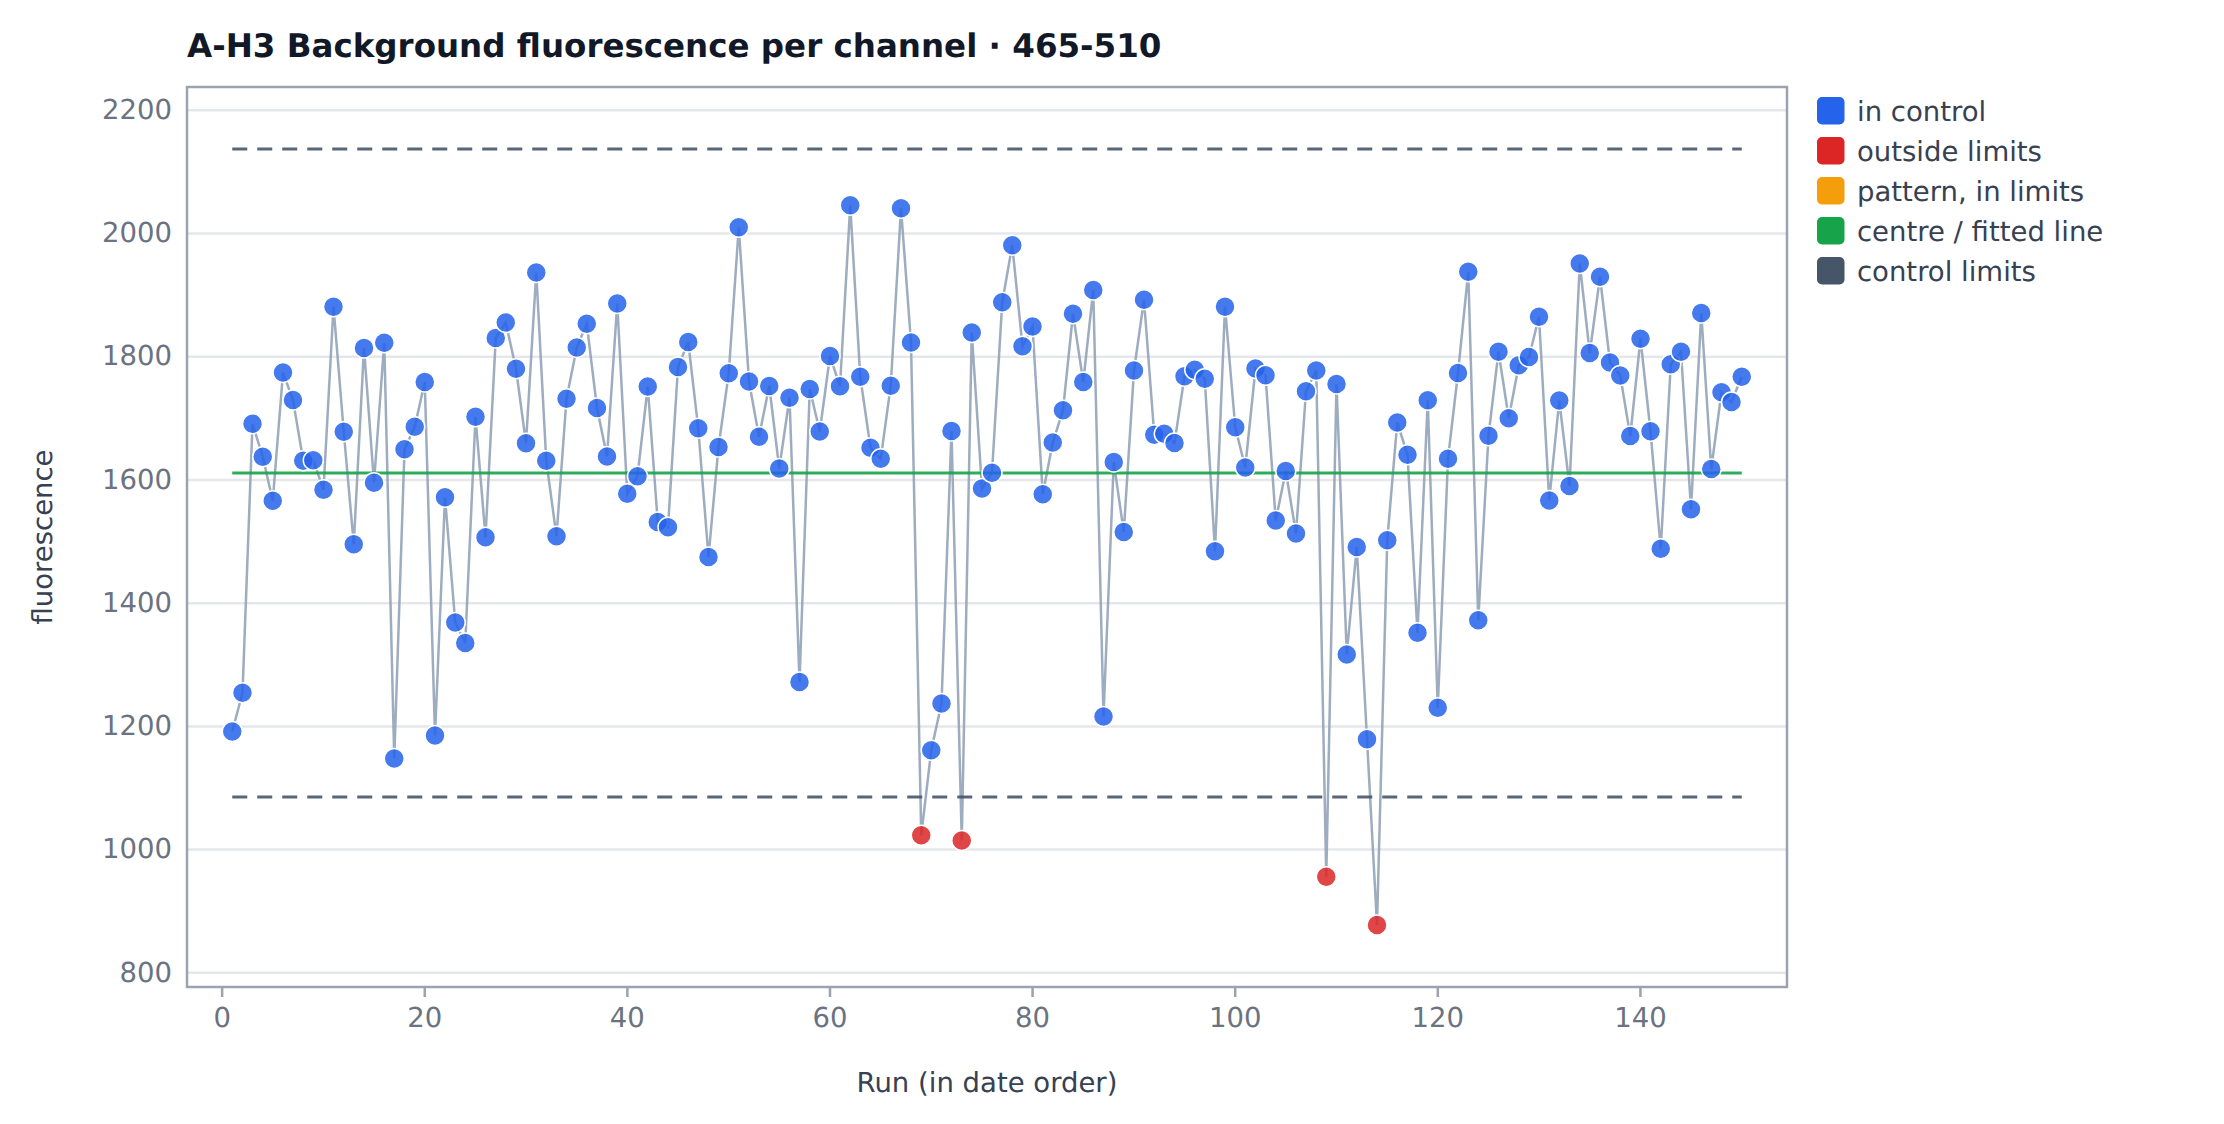
\includegraphics[width=0.82\textwidth]{fig/cc_bg_median_465_510.png}
\captionof{figure}{Example control chart used in the atlas.}
\end{center}

\clearpage
\includepdf[pages=-,fitpaper=true,landscape=true,pagecommand={\thispagestyle{empty}}]{fig/atlas_A4_landscape.pdf}


\chapter{Appendix I: Atlas manifest and source data}
\label{app:atlas-data}

Appendix~\ref{app:atlas-pages} contains the rendered A4 pages. This appendix records the source-file manifest and provenance without reproducing raw CSV listings: the CSV files are machine inputs for the chart renderer and are retained in the release ZIP.

\begin{itemize}
\item Source archive: \path{DEMO_control_charts_realscale.zip}.
\item 201 source CSV files correspond one-to-one with the 201 atlas pages.
\item The page renderer reads run key, value, centre line, limits, signal and interpretation fields directly from those files.
\item Values are synthetic demonstration data.
\end{itemize}

\begin{longtable}{@{}p{11cm}r@{}}\caption{A4 atlas data manifest.}\label{tab:atlas-manifest-i}\\
\toprule File & Rows\\\hline\endfirsthead\toprule File & Rows\\\hline\endhead
\path{001\_LC\_LC-DEMO-01\_00\_summary.csv} & 44\\\hline
\path{002\_LC\_LC-DEMO-01\_A-H3\_bg\_median\_465-510.csv} & 151\\\hline
\path{003\_LC\_LC-DEMO-01\_A-H3\_bg\_median\_533-580.csv} & 151\\\hline
\path{004\_LC\_LC-DEMO-01\_A-H3b\_plateau\_median\_465-510.csv} & 151\\\hline
\path{005\_LC\_LC-DEMO-01\_A-H3b\_plateau\_median\_533-580.csv} & 151\\\hline
\path{006\_LC\_LC-DEMO-01\_A-H4\_run\_minutes.csv} & 151\\\hline
\path{007\_LC\_LC-DEMO-01\_A-M1\_pc\_cq\_35S\_DEMO-CRM.csv} & 151\\\hline
\path{008\_LC\_LC-DEMO-01\_A-M1\_pc\_cq\_HMG\_DEMO-CRM.csv} & 151\\\hline
\path{009\_LC\_LC-DEMO-01\_A-M1\_pc\_cq\_T-NOS\_DEMO-CRM.csv} & 151\\\hline
\path{010\_LC\_LC-DEMO-01\_A-S4\_edit\_delay.csv} & 151\\\hline
\path{011\_LC\_LC-DEMO-01\_A-S6\_findings.csv} & 151\\\hline
\path{012\_LC\_LC-DEMO-01\_B-H11\_exposure\_465-510.csv} & 151\\\hline
\path{013\_LC\_LC-DEMO-01\_B-H11\_exposure\_533-580.csv} & 151\\\hline
\path{014\_LC\_LC-DEMO-01\_B-H17\_chan\_switch.csv} & 151\\\hline
\path{015\_LC\_LC-DEMO-01\_B-H1\_heat\_rate.csv} & 151\\\hline
\path{016\_LC\_LC-DEMO-01\_B-H2\_cool\_rate.csv} & 151\\\hline
\path{017\_LC\_LC-DEMO-01\_B-H3\_overshoot.csv} & 151\\\hline
\path{018\_LC\_LC-DEMO-01\_B-H3b\_settling.csv} & 151\\\hline
\path{019\_LC\_LC-DEMO-01\_B-H3c\_transition\_60-to-72.csv} & 151\\\hline
\path{020\_LC\_LC-DEMO-01\_B-H3c\_transition\_72-to-40.csv} & 151\\\hline
\path{021\_LC\_LC-DEMO-01\_B-H3c\_transition\_72-to-95.csv} & 151\\\hline
\path{022\_LC\_LC-DEMO-01\_B-H3c\_transition\_95-to-60.csv} & 151\\\hline
\path{023\_LC\_LC-DEMO-01\_B-H4\_hold\_temp.csv} & 151\\\hline
\path{024\_LC\_LC-DEMO-01\_B-H8\_lamp\_ref\_465-510.csv} & 151\\\hline
\path{025\_LC\_LC-DEMO-01\_B-H8\_lamp\_ref\_533-580.csv} & 151\\\hline
\path{026\_LC\_LC-DEMO-01\_B-H9\_lamp\_drift\_465-510.csv} & 151\\\hline
\path{027\_LC\_LC-DEMO-01\_B-H9\_lamp\_drift\_533-580.csv} & 151\\\hline
\path{028\_LC\_LC-DEMO-01\_B-M10\_late\_rate.csv} & 151\\\hline
\path{029\_LC\_LC-DEMO-01\_B-M1\_pc\_amplitude\_35S\_DEMO-CRM.csv} & 151\\\hline
\path{030\_LC\_LC-DEMO-01\_B-M1\_pc\_amplitude\_HMG\_DEMO-CRM.csv} & 151\\\hline
\path{031\_LC\_LC-DEMO-01\_B-M1\_pc\_amplitude\_T-NOS\_DEMO-CRM.csv} & 151\\\hline
\path{032\_LC\_LC-DEMO-01\_B-M5\_ntc\_rate\_legacy\_pooled\_stage\_unknown.csv} & 151\\\hline
\path{033\_LC\_LC-DEMO-01\_B-O11\_copied.csv} & 151\\\hline
\path{034\_LC\_LC-DEMO-01\_B-O1\_rep\_sd.csv} & 151\\\hline
\path{035\_LC\_LC-DEMO-01\_B-O3\_rowcol.csv} & 151\\\hline
\path{036\_LC\_LC-DEMO-01\_B-O5\_ntc\_op\_legacy\_pooled\_stage\_unknown.csv} & 4\\\hline
\path{037\_LC\_LC-DEMO-01\_B-O6\_action\_op.csv} & 4\\\hline
\path{038\_LC\_LC-DEMO-01\_B-O7\_manual\_rate.csv} & 151\\\hline
\path{039\_LC\_LC-DEMO-01\_B-O9\_call\_disagree.csv} & 151\\\hline
\path{040\_LC\_LC-DEMO-01\_B-S10\_templog\_late.csv} & 151\\\hline
\path{041\_LC\_LC-DEMO-01\_B-S11\_invalid\_acq.csv} & 151\\\hline
\path{042\_LC\_LC-DEMO-01\_B-S9\_cycle\_sd.csv} & 151\\\hline
\path{043\_LC\_LC-DEMO-01\_history.csv} & 151\\\hline
\path{044\_LC\_LC-DEMO-02\_00\_summary.csv} & 44\\\hline
\path{045\_LC\_LC-DEMO-02\_A-H3\_bg\_median\_465-510.csv} & 56\\\hline
\path{046\_LC\_LC-DEMO-02\_A-H3\_bg\_median\_533-580.csv} & 56\\\hline
\path{047\_LC\_LC-DEMO-02\_A-H3b\_plateau\_median\_465-510.csv} & 56\\\hline
\path{048\_LC\_LC-DEMO-02\_A-H3b\_plateau\_median\_533-580.csv} & 56\\\hline
\path{049\_LC\_LC-DEMO-02\_A-H4\_run\_minutes.csv} & 56\\\hline
\path{050\_LC\_LC-DEMO-02\_A-M1\_pc\_cq\_35S\_DEMO-CRM.csv} & 56\\\hline
\path{051\_LC\_LC-DEMO-02\_A-M1\_pc\_cq\_HMG\_DEMO-CRM.csv} & 56\\\hline
\path{052\_LC\_LC-DEMO-02\_A-M1\_pc\_cq\_T-NOS\_DEMO-CRM.csv} & 56\\\hline
\path{053\_LC\_LC-DEMO-02\_A-S4\_edit\_delay.csv} & 56\\\hline
\path{054\_LC\_LC-DEMO-02\_A-S6\_findings.csv} & 56\\\hline
\path{055\_LC\_LC-DEMO-02\_B-H11\_exposure\_465-510.csv} & 56\\\hline
\path{056\_LC\_LC-DEMO-02\_B-H11\_exposure\_533-580.csv} & 56\\\hline
\path{057\_LC\_LC-DEMO-02\_B-H17\_chan\_switch.csv} & 56\\\hline
\path{058\_LC\_LC-DEMO-02\_B-H1\_heat\_rate.csv} & 56\\\hline
\path{059\_LC\_LC-DEMO-02\_B-H2\_cool\_rate.csv} & 56\\\hline
\path{060\_LC\_LC-DEMO-02\_B-H3\_overshoot.csv} & 56\\\hline
\path{061\_LC\_LC-DEMO-02\_B-H3b\_settling.csv} & 56\\\hline
\path{062\_LC\_LC-DEMO-02\_B-H3c\_transition\_60-to-72.csv} & 56\\\hline
\path{063\_LC\_LC-DEMO-02\_B-H3c\_transition\_72-to-40.csv} & 56\\\hline
\path{064\_LC\_LC-DEMO-02\_B-H3c\_transition\_72-to-95.csv} & 56\\\hline
\path{065\_LC\_LC-DEMO-02\_B-H3c\_transition\_95-to-60.csv} & 56\\\hline
\path{066\_LC\_LC-DEMO-02\_B-H4\_hold\_temp.csv} & 56\\\hline
\path{067\_LC\_LC-DEMO-02\_B-H8\_lamp\_ref\_465-510.csv} & 56\\\hline
\path{068\_LC\_LC-DEMO-02\_B-H8\_lamp\_ref\_533-580.csv} & 56\\\hline
\path{069\_LC\_LC-DEMO-02\_B-H9\_lamp\_drift\_465-510.csv} & 56\\\hline
\path{070\_LC\_LC-DEMO-02\_B-H9\_lamp\_drift\_533-580.csv} & 56\\\hline
\path{071\_LC\_LC-DEMO-02\_B-M10\_late\_rate.csv} & 56\\\hline
\path{072\_LC\_LC-DEMO-02\_B-M1\_pc\_amplitude\_35S\_DEMO-CRM.csv} & 56\\\hline
\path{073\_LC\_LC-DEMO-02\_B-M1\_pc\_amplitude\_HMG\_DEMO-CRM.csv} & 56\\\hline
\path{074\_LC\_LC-DEMO-02\_B-M1\_pc\_amplitude\_T-NOS\_DEMO-CRM.csv} & 56\\\hline
\path{075\_LC\_LC-DEMO-02\_B-M5\_ntc\_rate\_legacy\_pooled\_stage\_unknown.csv} & 56\\\hline
\path{076\_LC\_LC-DEMO-02\_B-O11\_copied.csv} & 56\\\hline
\path{077\_LC\_LC-DEMO-02\_B-O1\_rep\_sd.csv} & 56\\\hline
\path{078\_LC\_LC-DEMO-02\_B-O3\_rowcol.csv} & 56\\\hline
\path{079\_LC\_LC-DEMO-02\_B-O5\_ntc\_op\_legacy\_pooled\_stage\_unknown.csv} & 4\\\hline
\path{080\_LC\_LC-DEMO-02\_B-O6\_action\_op.csv} & 4\\\hline
\path{081\_LC\_LC-DEMO-02\_B-O7\_manual\_rate.csv} & 56\\\hline
\path{082\_LC\_LC-DEMO-02\_B-O9\_call\_disagree.csv} & 48\\\hline
\path{083\_LC\_LC-DEMO-02\_B-S10\_templog\_late.csv} & 56\\\hline
\path{084\_LC\_LC-DEMO-02\_B-S11\_invalid\_acq.csv} & 56\\\hline
\path{085\_LC\_LC-DEMO-02\_B-S9\_cycle\_sd.csv} & 56\\\hline
\path{086\_LC\_LC-DEMO-02\_history.csv} & 56\\\hline
\path{087\_QS\_QS-DEMO-A\_00\_summary.csv} & 65\\\hline
\path{088\_QS\_QS-DEMO-A\_A-H3\_bg\_median\_x1-m1.csv} & 91\\\hline
\path{089\_QS\_QS-DEMO-A\_A-H3\_bg\_median\_x2-m2.csv} & 91\\\hline
\path{090\_QS\_QS-DEMO-A\_A-H3b\_plateau\_median\_x1-m1.csv} & 91\\\hline
\path{091\_QS\_QS-DEMO-A\_A-H3b\_plateau\_median\_x2-m2.csv} & 91\\\hline
\path{092\_QS\_QS-DEMO-A\_A-H4\_run\_minutes.csv} & 91\\\hline
\path{093\_QS\_QS-DEMO-A\_A-S4\_edit\_delay.csv} & 91\\\hline
\path{094\_QS\_QS-DEMO-A\_A-S6\_findings.csv} & 91\\\hline
\path{095\_QS\_QS-DEMO-A\_B-H10\_led\_current.csv} & 91\\\hline
\path{096\_QS\_QS-DEMO-A\_B-H10b\_led\_junction.csv} & 91\\\hline
\path{097\_QS\_QS-DEMO-A\_B-H11\_exposure\_x1-m1.csv} & 91\\\hline
\path{098\_QS\_QS-DEMO-A\_B-H11\_exposure\_x1-m2.csv} & 91\\\hline
\path{099\_QS\_QS-DEMO-A\_B-H11\_exposure\_x2-m2.csv} & 91\\\hline
\path{100\_QS\_QS-DEMO-A\_B-H11\_exposure\_x2-m3.csv} & 91\\\hline
\path{101\_QS\_QS-DEMO-A\_B-H11\_exposure\_x3-m3.csv} & 91\\\hline
\path{102\_QS\_QS-DEMO-A\_B-H11\_exposure\_x3-m4.csv} & 91\\\hline
\path{103\_QS\_QS-DEMO-A\_B-H11\_exposure\_x4-m4.csv} & 91\\\hline
\path{104\_QS\_QS-DEMO-A\_B-H11\_exposure\_x5-m5.csv} & 91\\\hline
\path{105\_QS\_QS-DEMO-A\_B-H12\_saturation.csv} & 91\\\hline
\path{106\_QS\_QS-DEMO-A\_B-H13\_calib\_uniformity.csv} & 91\\\hline
\path{107\_QS\_QS-DEMO-A\_B-H13b\_calib\_background.csv} & 91\\\hline
\path{108\_QS\_QS-DEMO-A\_B-H13c\_calib\_roi.csv} & 91\\\hline
\path{109\_QS\_QS-DEMO-A\_B-H14\_wheel\_ms.csv} & 91\\\hline
\path{110\_QS\_QS-DEMO-A\_B-H14b\_wheel\_slow.csv} & 91\\\hline
\path{111\_QS\_QS-DEMO-A\_B-H15\_encoder\_emission.csv} & 91\\\hline
\path{112\_QS\_QS-DEMO-A\_B-H15\_encoder\_excitation.csv} & 91\\\hline
\path{113\_QS\_QS-DEMO-A\_B-H16\_cam\_overhead.csv} & 91\\\hline
\path{114\_QS\_QS-DEMO-A\_B-H18\_cover\_down.csv} & 91\\\hline
\path{115\_QS\_QS-DEMO-A\_B-H18b\_cover\_up.csv} & 91\\\hline
\path{116\_QS\_QS-DEMO-A\_B-H1\_heat\_rate.csv} & 91\\\hline
\path{117\_QS\_QS-DEMO-A\_B-H2\_cool\_rate.csv} & 91\\\hline
\path{118\_QS\_QS-DEMO-A\_B-H3c\_transition\_60-to-95.csv} & 91\\\hline
\path{119\_QS\_QS-DEMO-A\_B-H3c\_transition\_95-to-60.csv} & 91\\\hline
\path{120\_QS\_QS-DEMO-A\_B-H5\_zone\_spread.csv} & 91\\\hline
\path{121\_QS\_QS-DEMO-A\_B-H6\_heatsink\_max.csv} & 91\\\hline
\path{122\_QS\_QS-DEMO-A\_B-H6b\_cover\_temp.csv} & 91\\\hline
\path{123\_QS\_QS-DEMO-A\_B-M10\_late\_rate.csv} & 91\\\hline
\path{124\_QS\_QS-DEMO-A\_B-M2\_rox\_level.csv} & 91\\\hline
\path{125\_QS\_QS-DEMO-A\_B-M9\_low\_conf.csv} & 91\\\hline
\path{126\_QS\_QS-DEMO-A\_B-O11\_copied.csv} & 91\\\hline
\path{127\_QS\_QS-DEMO-A\_B-O1\_rep\_sd.csv} & 91\\\hline
\path{128\_QS\_QS-DEMO-A\_B-O2\_rox\_cv.csv} & 91\\\hline
\path{129\_QS\_QS-DEMO-A\_B-O3\_rowcol.csv} & 91\\\hline
\path{130\_QS\_QS-DEMO-A\_B-O6\_action\_op.csv} & 4\\\hline
\path{131\_QS\_QS-DEMO-A\_B-O7\_manual\_rate.csv} & 91\\\hline
\path{132\_QS\_QS-DEMO-A\_B-O9\_call\_disagree.csv} & 91\\\hline
\path{133\_QS\_QS-DEMO-A\_B-S12\_ct\_mismatch.csv} & 91\\\hline
\path{134\_QS\_QS-DEMO-A\_B-S1\_cmd\_rt.csv} & 91\\\hline
\path{135\_QS\_QS-DEMO-A\_B-S2\_tick\_late.csv} & 91\\\hline
\path{136\_QS\_QS-DEMO-A\_B-S2b\_catch\_up.csv} & 91\\\hline
\path{137\_QS\_QS-DEMO-A\_B-S3\_img\_proc.csv} & 91\\\hline
\path{138\_QS\_QS-DEMO-A\_B-S5\_runtime\_err.csv} & 91\\\hline
\path{139\_QS\_QS-DEMO-A\_B-S6\_handoff\_min.csv} & 91\\\hline
\path{140\_QS\_QS-DEMO-A\_B-S8\_log\_errors.csv} & 91\\\hline
\path{141\_QS\_QS-DEMO-A\_B-S9\_cycle\_sd.csv} & 91\\\hline
\path{142\_QS\_QS-DEMO-A\_history.csv} & 91\\\hline
\path{143\_QS\_QS-DEMO-B\_00\_summary.csv} & 69\\\hline
\path{144\_QS\_QS-DEMO-B\_A-H3\_bg\_median\_x1-m1.csv} & 31\\\hline
\path{145\_QS\_QS-DEMO-B\_A-H3\_bg\_median\_x2-m2.csv} & 31\\\hline
\path{146\_QS\_QS-DEMO-B\_A-H3\_bg\_median\_x3-m3.csv} & 31\\\hline
\path{147\_QS\_QS-DEMO-B\_A-H3\_bg\_median\_x4-m4.csv} & 31\\\hline
\path{148\_QS\_QS-DEMO-B\_A-H3b\_plateau\_median\_x1-m1.csv} & 31\\\hline
\path{149\_QS\_QS-DEMO-B\_A-H3b\_plateau\_median\_x2-m2.csv} & 31\\\hline
\path{150\_QS\_QS-DEMO-B\_A-H3b\_plateau\_median\_x3-m3.csv} & 31\\\hline
\path{151\_QS\_QS-DEMO-B\_A-H3b\_plateau\_median\_x4-m4.csv} & 31\\\hline
\path{152\_QS\_QS-DEMO-B\_A-H4\_run\_minutes.csv} & 31\\\hline
\path{153\_QS\_QS-DEMO-B\_A-S4\_edit\_delay.csv} & 31\\\hline
\path{154\_QS\_QS-DEMO-B\_A-S6\_findings.csv} & 31\\\hline
\path{155\_QS\_QS-DEMO-B\_B-H10\_led\_current.csv} & 31\\\hline
\path{156\_QS\_QS-DEMO-B\_B-H10b\_led\_junction.csv} & 31\\\hline
\path{157\_QS\_QS-DEMO-B\_B-H11\_exposure\_x1-m1.csv} & 31\\\hline
\path{158\_QS\_QS-DEMO-B\_B-H11\_exposure\_x1-m2.csv} & 31\\\hline
\path{159\_QS\_QS-DEMO-B\_B-H11\_exposure\_x2-m2.csv} & 31\\\hline
\path{160\_QS\_QS-DEMO-B\_B-H11\_exposure\_x2-m3.csv} & 31\\\hline
\path{161\_QS\_QS-DEMO-B\_B-H11\_exposure\_x3-m3.csv} & 31\\\hline
\path{162\_QS\_QS-DEMO-B\_B-H11\_exposure\_x3-m4.csv} & 31\\\hline
\path{163\_QS\_QS-DEMO-B\_B-H11\_exposure\_x4-m4.csv} & 31\\\hline
\path{164\_QS\_QS-DEMO-B\_B-H11\_exposure\_x5-m5.csv} & 31\\\hline
\path{165\_QS\_QS-DEMO-B\_B-H12\_saturation.csv} & 31\\\hline
\path{166\_QS\_QS-DEMO-B\_B-H13\_calib\_uniformity.csv} & 31\\\hline
\path{167\_QS\_QS-DEMO-B\_B-H13b\_calib\_background.csv} & 31\\\hline
\path{168\_QS\_QS-DEMO-B\_B-H13c\_calib\_roi.csv} & 31\\\hline
\path{169\_QS\_QS-DEMO-B\_B-H14\_wheel\_ms.csv} & 31\\\hline
\path{170\_QS\_QS-DEMO-B\_B-H14b\_wheel\_slow.csv} & 31\\\hline
\path{171\_QS\_QS-DEMO-B\_B-H15\_encoder\_emission.csv} & 31\\\hline
\path{172\_QS\_QS-DEMO-B\_B-H15\_encoder\_excitation.csv} & 31\\\hline
\path{173\_QS\_QS-DEMO-B\_B-H16\_cam\_overhead.csv} & 31\\\hline
\path{174\_QS\_QS-DEMO-B\_B-H18\_cover\_down.csv} & 31\\\hline
\path{175\_QS\_QS-DEMO-B\_B-H18b\_cover\_up.csv} & 31\\\hline
\path{176\_QS\_QS-DEMO-B\_B-H1\_heat\_rate.csv} & 31\\\hline
\path{177\_QS\_QS-DEMO-B\_B-H2\_cool\_rate.csv} & 31\\\hline
\path{178\_QS\_QS-DEMO-B\_B-H3c\_transition\_60-to-95.csv} & 31\\\hline
\path{179\_QS\_QS-DEMO-B\_B-H3c\_transition\_95-to-60.csv} & 31\\\hline
\path{180\_QS\_QS-DEMO-B\_B-H5\_zone\_spread.csv} & 31\\\hline
\path{181\_QS\_QS-DEMO-B\_B-H6\_heatsink\_max.csv} & 31\\\hline
\path{182\_QS\_QS-DEMO-B\_B-H6b\_cover\_temp.csv} & 31\\\hline
\path{183\_QS\_QS-DEMO-B\_B-M10\_late\_rate.csv} & 31\\\hline
\path{184\_QS\_QS-DEMO-B\_B-M2\_rox\_level.csv} & 31\\\hline
\path{185\_QS\_QS-DEMO-B\_B-M9\_low\_conf.csv} & 31\\\hline
\path{186\_QS\_QS-DEMO-B\_B-O11\_copied.csv} & 31\\\hline
\path{187\_QS\_QS-DEMO-B\_B-O1\_rep\_sd.csv} & 31\\\hline
\path{188\_QS\_QS-DEMO-B\_B-O2\_rox\_cv.csv} & 31\\\hline
\path{189\_QS\_QS-DEMO-B\_B-O3\_rowcol.csv} & 31\\\hline
\path{190\_QS\_QS-DEMO-B\_B-O6\_action\_op.csv} & 4\\\hline
\path{191\_QS\_QS-DEMO-B\_B-O7\_manual\_rate.csv} & 31\\\hline
\path{192\_QS\_QS-DEMO-B\_B-S12\_ct\_mismatch.csv} & 31\\\hline
\path{193\_QS\_QS-DEMO-B\_B-S1\_cmd\_rt.csv} & 31\\\hline
\path{194\_QS\_QS-DEMO-B\_B-S2\_tick\_late.csv} & 31\\\hline
\path{195\_QS\_QS-DEMO-B\_B-S2b\_catch\_up.csv} & 31\\\hline
\path{196\_QS\_QS-DEMO-B\_B-S3\_img\_proc.csv} & 31\\\hline
\path{197\_QS\_QS-DEMO-B\_B-S5\_runtime\_err.csv} & 31\\\hline
\path{198\_QS\_QS-DEMO-B\_B-S6\_handoff\_min.csv} & 31\\\hline
\path{199\_QS\_QS-DEMO-B\_B-S8\_log\_errors.csv} & 31\\\hline
\path{200\_QS\_QS-DEMO-B\_B-S9\_cycle\_sd.csv} & 31\\\hline
\path{201\_QS\_QS-DEMO-B\_history.csv} & 31\\\hline
\end{longtable}


\end{document}





